\documentclass[aspectratio=169, 9pt]{beamer}
\usepackage{caption}
\usepackage{subcaption}
\usepackage{braket}
%
\usepackage{amsmath}
%%%%%%%%%%%%%%%%%%%
\newcommand{\Eins}{\mathds{1}}

\usepackage[normalem]{ulem}
\usepackage{tikz}

\def\clap#1{\hbox to 0pt{\hss#1\hss}}
\def\mathllap{\mathpalette\mathllapinternal}
\def\mathrlap{\mathpalette\mathrlapinternal}
\def\mathclap{\mathpalette\mathclapinternal}
\def\mathllapinternal#1#2{%
\llap{$\mathsurround=0pt#1{#2}$}}
\def\mathrlapinternal#1#2{%
\rlap{$\mathsurround=0pt#1{#2}$}}
\def\mathclapinternal#1#2{%
\clap{$\mathsurround=0pt#1{#2}$}}


\newcommand{\bc}{\begin{center}}
\newcommand{\ec}{\end{center}}
\def\t0{t\text{$=$}0}
\def\ix0{\xi\text{$=$}0}
%\def\wg{\stackrel{\text{\scriptsize{worm}}}{\text{\scriptsize{gear}}}}
\def\wg{{g_{1T}}}

\newcommand{\bea}{\vspace{-0mm}\begin{eqnarray}}
\newcommand{\eea}{\end{eqnarray}}
\newcommand{\Dlr}{{D^{\hspace{-0.8em}%
      \raisebox{0.8ex}{$\scriptstyle\leftrightarrow$}}}{}}
\newcommand{\Dl}{{D^{\hspace{-0.8em}%
      \raisebox{0.8ex}{$\scriptstyle\leftarrow$}}}{}}
\newcommand{\Dr}{{D^{\hspace{-0.8em}%
      \raisebox{0.8ex}{$\scriptstyle\rightarrow$}}}{}}
%
\newcommand{\gev}{\operatorname{GeV}}
\newcommand{\mev}{\operatorname{MeV}}
\newcommand{\fm}{\operatorname{fm}}
\usepackage{graphicx}
\newcommand{\ms}{\mskip 1.5mu}

\newcommand{\toolkit}[1]{{\tt #1}}

% editing markup, old version:
%\newcommand{\todo}[1]{$\langle$\textbf{TODO:} \emph{#1}$\rangle$}
%\newcommand{\muline}[1]{\uline{#1}}
%\newcommand{\mxout}[1]{\xout{#1}}
%\newcommand{\bnew}{$\langle$\textbf{new:}$\rangle$}
%\newcommand{\enew}{$\langle$\textbf{endnew}$\rangle$}
%\newcommand{\red}[1]{\textcolor{red}{[ #1 ]}}

% editing markup:
\newcommand{\TD}[1]{$\langle$\textbf{TODO:} \emph{#1}$\rangle$}
\newcommand{\todo}[1]{$\langle$\textbf{TODO:} \emph{#1}$\rangle$}
\newcommand{\muline}[1]{{\color{red!50!black}{#1}}}
\newcommand{\mxout}[1]{{\color{black!20!white}{#1}}}
\newcommand{\bnew}{$\langle$\textbf{new:}$\rangle$}
\newcommand{\enew}{$\langle$\textbf{endnew}$\rangle$}
\newcommand{\editnote}[1]{\marginpar{{\color{green!50!black}{#1}}}}


% editing markup deactivated:
%\newcommand{\todo}[1]{}
%\newcommand{\muline}[1]{#1}
%\newcommand{\mxout}[1]{}
%\newcommand{\bnew}{}
%\newcommand{\enew}{}

\newcommand{\units}[1]{\ensuremath{\,\mathrm{#1}}}
\newcommand{\braKet}[3]{#3\langle#1#3|#2#3\rangle}
\newcommand{\Tr}{\mathrm{tr}}
\newcommand{\BTr}{\mathrm{Tr}}
\newcommand{\elll}{{\color{red}l}}
\newcommand{\latcfn}{\ensuremath{C}}
\usepackage{graphicx}
\newcommand{\tpm}{\ensuremath{{\,\pm\,}}}

\newcommand{\prp}{\perp}
\newcommand{\transp}{\mathsf{T}}
\newcommand{\GammaOp}{\Gamma}
\newcommand{\GammaDist}{\ensuremath{\Gamma^\text{d}}}
\newcommand{\GammaTwo}{\ensuremath{\Gamma^\text{2pt}}}
\newcommand{\GammaThr}{\ensuremath{\Gamma^\text{3pt}}}
\newcommand{\GammaDiq}{\ensuremath{\Gamma^\text{diq}}}
\newcommand{\lat}{{\text{lat}}}
\newcommand{\ren}{{\text{ren}}}
\newcommand{\unren}{{\text{unren}}}
\newcommand{\norm}{{\text{norm}}}
\newcommand{\tcdot}{{\cdot}}
\newcommand{\ldotP}{{\elll\!\cdot\!P}}

\newcommand{\myRe}{\ensuremath{\mathrm{Re}}}
\newcommand{\myIm}{\ensuremath{\mathrm{Im}}}

\newcommand{\dlangle}{{\rlap{\big\langle}\hskip 0.1em\big\langle}}
\newcommand{\drangle}{{\rlap{\big\rangle}\hskip 0.1em\big\rangle}}

\newcommand{\Wline}[1]{\ensuremath{{\mathcal{U}}[#1]}}
\newcommand{\WlineC}[1]{\ensuremath{{\mathcal{U}}{[#1]}}}
\newcommand{\WlineClat}[1]{\ensuremath{{\mathcal{U}}^\text{lat}{[#1]}}}
\newcommand{\WlineI}[2]{\ensuremath{{\mathcal{U}}#1{[#2]}}}
\newcommand{\Wlineren}[1]{\ensuremath{{\mathcal{U}}^\text{ren}[#1]}}

\newcommand{\mean}[1]{\ensuremath{\left\langle{#1}\right\rangle}}
\newcommand{\vect}[1]{\ensuremath{\boldsymbol{#1}}}
\newcommand{\vprp}[1]{\vect{#1}_{\mathrm T}}

\newcommand{\mmin}{{\text{min}}}

\newcommand{\quark}{q}
\newcommand{\nucl}[1]{{#1}}
\newcommand{\Quark}{Q}
\newcommand{\Afield}{A}

\newcommand{\MDM}{\mathcal{M}}
\newcommand{\tMDM}{\tilde{\mathcal{M}}}
\newcommand{\tAmp}{\widetilde{A}}
\newcommand{\tBmp}{\widetilde{B}}
\newcommand{\TFM}{{\hat{\mathbb{T}}}}
\newcommand{\renZ}{Z}

%\newcommand{\len}{\mathcal{L}}
\newcommand{\len}{\ell}

\newcommand{\nplus}{\ensuremath{\bar n}}
\newcommand{\nminus}{\ensuremath{n}}


\newcommand{\TMD}{TMD\xspace}
\newcommand{\TMDs}{TMDs\xspace}

\newcommand{\sW}{\ensuremath{\text{sW}}}

\newcommand{\toddmark}[1]{\ensuremath{\Bigg[#1\Bigg]_{\text{\tiny{odd}}}}}
\newcommand{\Eu}[1]{#1}

\newcommand{\fourint}{\ensuremath{\int_\mathcal{F}}}
\newcommand{\xfourint}{\ensuremath{\int_\mathcal{M}}}


\newcommand{\conherm}{\ensuremath{(\dagger)}}
\newcommand{\conpar}{\ensuremath{(\mathrm{P})}}
\newcommand{\contime}{\ensuremath{(\mathrm{T})}}
\newcommand{\myeps}{\ensuremath{\epsilon}}

\newcommand{\xmom}[1]{{\ensuremath{[#1]}}}
\newcommand{\ktmom}[1]{{\ensuremath{(#1)}}}
\newcommand{\xktmom}[2]{{\xmom{#1}\ktmom{#2}}}

\newcommand{\bvec}{b}
\newcommand{\softf}{\mathcal{S}}
\newcommand{\mN}{m_N}
\newcommand{\nf}{n_f}


\newcommand{\sgn}{\mathrm{sgn}}
\newcommand{\nbdash}{\protect\nobreakdash-\hspace{0pt}}

\newcounter{fnnumber}
\newcounter{fnnumberamp}
\newcommand{\MSbar}{\overline{\text{MS}}}

\newcommand{\kei}{k}

\newcommand{\unsub}{\text{unsubtr.}}
\newcommand{\zetahat}{{\hat \zeta}}

%%%%%%%%%%%%%%%%%%%
% Choose how your presentation looks.
%
% For more themes, color themes and font themes, see:
% http://deic.uab.es/~iblanes/beamer_gallery/index_by_theme.html
%
\mode<presentation>
{
  \usetheme{Boadilla}      % or try Darmstadt, Madrid, Warsaw, ...
  \usecolortheme{default} % or try albatross, beaver, crane, ...
  \usefonttheme{serif}  % or try serif, structurebold, ...
  \setbeamertemplate{navigation symbols}{}
  \setbeamertemplate{caption}[numbered]
} 

\usepackage[english]{babel}
\usepackage[utf8]{inputenc}
\usepackage[T1]{fontenc}

%%%%%%%%%%%%%%%%%%%
% Defense additions
\usepackage{appendixnumberbeamer}
\usepackage{booktabs}
\usepackage{pifont}
\usepackage{xcolor}
\usetikzlibrary{arrows.meta,positioning,calc,decorations.pathmorphing,shapes.geometric}
\graphicspath{{figures/thesis/}{figures/template/}}
\newcommand{\keymsg}[1]{\begin{block}{}\centering #1\end{block}}
\newcommand{\figsrc}[1]{\par\vspace{-1mm}{\tiny\color{gray}#1}}
\definecolor{okgreen}{RGB}{0,128,60}
\definecolor{badred}{RGB}{190,30,30}
% small grey tag for slides meant to be shown quickly
\newcommand{\quick}{\begin{tikzpicture}[remember picture,overlay]\node[anchor=north east, font=\tiny, text=gray, inner sep=2pt] at ([xshift=-1mm,yshift=-1mm]current page.north east) {quick};\end{tikzpicture}}

\title[\texorpdfstring{$x$}{x}-dependence of the Sivers shift from lattice QCD]{\textbf{Dependence of the Sivers TMD Shift on\\ Quark Longitudinal Momentum Fraction \texorpdfstring{$x$}{x}\\ from Lattice QCD}}
\subtitle{~\\ PhD Dissertation Defense}
% Committee as listed in the thesis approval page (approval.tex)
\author[Hariprashad Ravikumar]
{\texorpdfstring{\textbf{Hariprashad Ravikumar}\inst{$\dagger$}\\~\\
 Doctoral Advisor (Chair): \textbf{Dr. Michael Engelhardt}\inst{$\dagger$}\\[1mm]
 Doctoral Committee: \textbf{Dr. Mathew Sievert}\inst{$\dagger$}, \textbf{Dr. Ludi Miao}\inst{$\dagger$}, \textbf{Dr. Tuan Le}\inst{$\dagger$}}{Hariprashad Ravikumar}}
\institute[NMSU]{\inst{$\dagger$}Department of Physics, New Mexico State University, USA}
\date[]{October 23, 2026} % TODO(Hari): set the exact defense date

\begin{document}

\begin{frame}
  \titlepage
  \vspace{-4mm}
  \begin{center}
    
\includegraphics[scale=0.15]{NMSU_BBStF-Left.eps}
  \end{center}
\end{frame}

% ===================== 0. Opening =====================
% Slide 2 -- the question, and a preview of the answer (revisited on the headline slide)

\begin{frame}{The question of this thesis}
  \begin{columns}[c]
    \begin{column}{0.42\textwidth}
      \begin{itemize}
        \item In a transversely polarized proton, unpolarized quarks are pushed \textbf{sideways}: the \textbf{Sivers effect}.
        \item Lattice QCD has computed the size of this push, but only \textbf{integrated over the momentum fraction $x$}.
        \item[]
        \item \textbf{Question:} can lattice QCD give the Sivers shift \textbf{as a function of $x$}?
      \end{itemize}
      \vspace{3mm}
      \keymsg{Where we are going: the Sivers shift as a function of $x$}
    \end{column}
    \begin{column}{0.56\textwidth}
      \centering
      \begin{tikzpicture}
        \node[opacity=0.35, inner sep=0pt] (img) {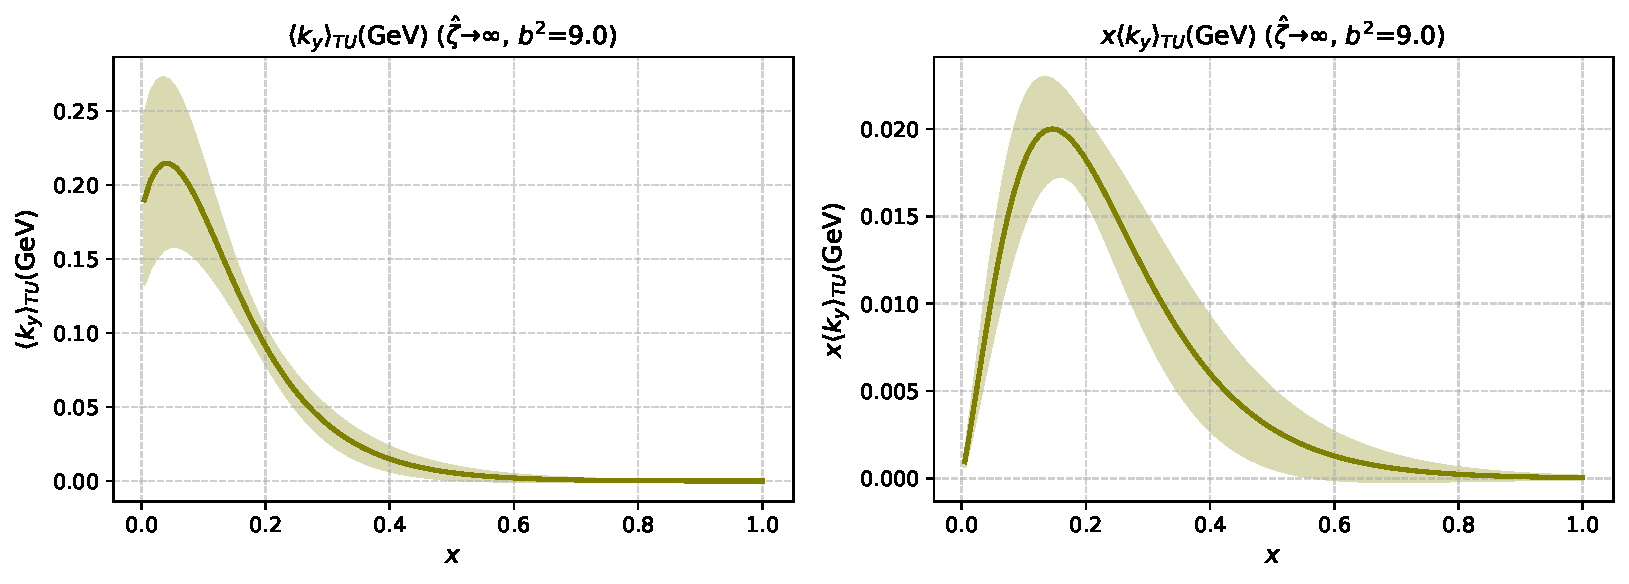
\includegraphics[width=\linewidth]{Extrapolated_AmpLevel_P234_Sivers_1_over_zetahat_sq_bmin3_eta610_b29.0_Sivers.pdf}};
        \node[draw=gray, fill=white, rounded corners, font=\large, anchor=south] at ([yshift=2mm]img.north) {\textbf{?}\ \ answer at the end};
      \end{tikzpicture}
    \end{column}
  \end{columns}
\end{frame}

% ===================== I. Motivation =====================
\section{Motivation}

% Slide 3
\begin{frame}{From parton distributions to 3D tomography}
  \begin{columns}[c]
    \begin{column}{0.40\textwidth}
      \begin{itemize}
        \item Deep inelastic scattering: a quark carries the light-cone momentum fraction
        \[ x = \frac{k^+}{P^+} \]
        \item Collinear PDFs $f_1(x)$ are a \textbf{1D} picture.
        \item \textbf{TMDs} keep the transverse momentum $\vprp{k}$: momentum-space tomography.
        \item TMDs need semi-inclusive processes (SIDIS, Drell--Yan).
      \end{itemize}
    \end{column}
    \begin{column}{0.58\textwidth}
      \centering
      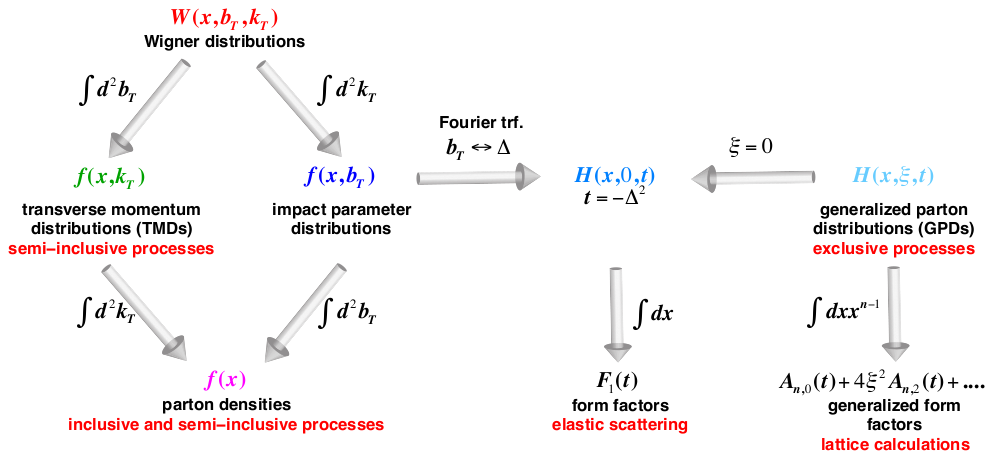
\includegraphics[width=\linewidth]{EIC_WP_Fig2p2_distributions.png}
      \figsrc{Adapted from Accardi \emph{et al.}, EPJA \textbf{52}, 268 (2016)}
    \end{column}
  \end{columns}
\end{frame}

\begin{frame}{Transverse position and transverse momentum}
  \begin{columns}[c]
  \begin{column}{0.55\textwidth}
  \begin{itemize}
    \item GPDs encode transverse position, through Fourier transformation of transverse momentum transfer $\vect\Delta_T$.
    \item TMDs encode the quark transverse momentum $\vect k_T$.
    \item The impact parameter in this picture is distinct from the quark-field separation $\vect b_T$ used in the TMD correlator.
  \end{itemize}
  \[ \rho_q(x,\vect b_T)=\int\frac{d^2\vect\Delta_T}{(2\pi)^2}
       e^{-i\vect b_T\cdot\vect\Delta_T}H^q(x,0,-\vect\Delta_T^2). \]
  \end{column}
  \begin{column}{0.41\textwidth}\centering
    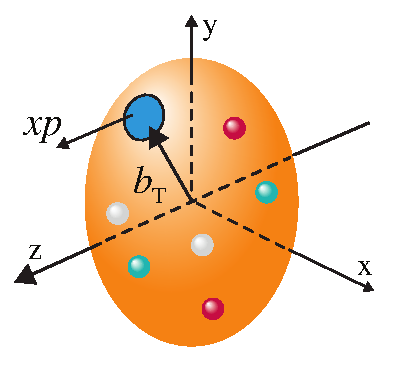
\includegraphics[width=\linewidth,height=0.65\textheight,keepaspectratio]{EIC_WP_Fig2p1_parton_bT.pdf}
  \end{column}
  \end{columns}
  \figsrc{Thesis, Ch. 2; Accardi et al., EPJA 52, 268 (2016), arXiv:1212.1701, Fig. 2.1 (CC BY 4.0).}
\end{frame}

\begin{frame}{Leading-twist quark TMDs}
  \centering\renewcommand{\arraystretch}{1.65}
  \begin{tabular}{c|ccc}
    Nucleon $\backslash$ quark & unpolarized & longitudinal & transverse\\\hline
    Unpolarized & $f_1$ & & $h_1^\perp$ (T-odd)\\
    Longitudinal & & $g_1$ & $h_{1L}^\perp$\\
    Transverse & $f_{1T}^\perp$ (T-odd) & $g_{1T}$ & $h_1,\ h_{1T}^\perp$
  \end{tabular}
  \vspace{4mm}
  \begin{itemize}
    \item The Sivers function describes unpolarized quarks in a transversely polarized nucleon.
    \item Sivers and Boer--Mulders functions change sign between future- and past-pointing staple links.
  \end{itemize}
  \figsrc{Thesis, Ch. 2: leading-twist quark TMD polarization table.}
\end{frame}

% Slide 4
\begin{frame}{Single-spin asymmetries and the Sivers effect}
  \begin{columns}[c]
    \begin{column}{0.48\textwidth}
      \begin{itemize}
        \item Large left--right asymmetries off transversely polarized protons (E704, 1991).
        \item Leading-twist collinear hard-scattering estimates predict tiny asymmetries (Kane, Pumplin, Repko 1978).
        \item Sivers (1990): the quark $\vprp{k}$ distribution is \textbf{shifted perpendicular to the spin}.
      \end{itemize}
      \vspace{-1mm}
      \[ f_{q/N^\uparrow}(x,\vprp{k}) = f_1^q(x,\vprp{k}^2) - \frac{\epsilon_{ij}\,k_{T,i}\,S_{T,j}}{\mN}\, f_{1T}^{\perp q}(x,\vprp{k}^2) \]
      \centering
      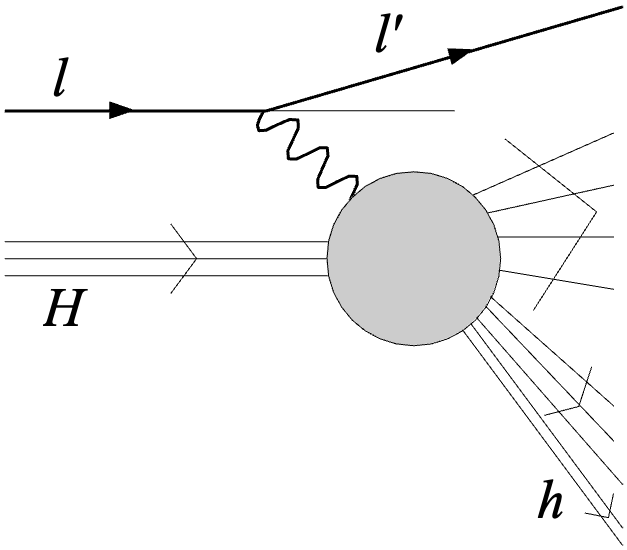
\includegraphics[width=0.42\linewidth]{SIDIS.png}\\
      {\tiny SIDIS: $\ell N^\uparrow\to\ell' h X$}
    \end{column}
    \begin{column}{0.50\textwidth}
      \centering
      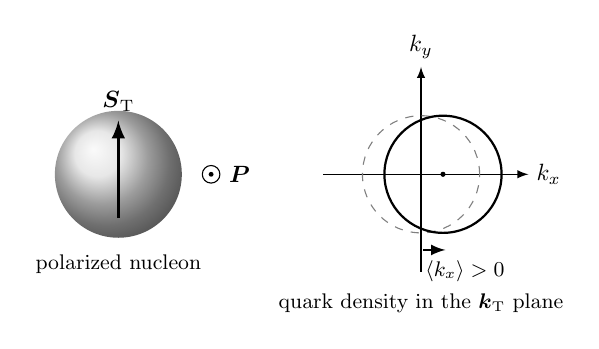
\begin{tikzpicture}[scale=0.62, every node/.style={scale=0.85}]
        \begin{scope}[shift={(-3.2,0)}]
          \shade[ball color=gray!25] (0,0) circle (1.3);
          \draw[very thick, -latex] (0,-0.9) -- (0,1.1) node[above] {$\vprp{S}$};
          \draw (1.9,0) circle (0.18); \fill (1.9,0) circle (0.05);
          \node[right] at (2.1,0) {$\vect{P}$};
          \node at (0,-1.85) {\small polarized nucleon};
        \end{scope}
        \begin{scope}[shift={(3.0,0)}]
          \draw[-latex] (-2.0,0) -- (2.2,0) node[right] {$k_x$};
          \draw[-latex] (0,-2.0) -- (0,2.2) node[above] {$k_y$};
          \draw[dashed, gray] (0,0) circle (1.2);
          \draw[thick] (0.45,0) circle (1.2);
          \fill (0.45,0) circle (1.5pt);
          \draw[-latex, thick] (0.05,-1.55) -- (0.5,-1.55);
          \node[below] at (0.9,-1.6) {\small $\langle k_x\rangle > 0$};
          \node at (0,-2.65) {\small quark density in the $\vprp{k}$ plane};
        \end{scope}
      \end{tikzpicture}
      \\[1mm]
      {\scriptsize $\vect{P}$ out of the page, $\vprp{S}\parallel\hat y$: the shift is along $\hat x$ (shown: $f_{1T}^\perp<0$).\\
      In the Sivers-shift definition $\vprp{S}\parallel\hat x$ and we measure $\langle k_y\rangle$.}
    \end{column}
  \end{columns}
\end{frame}

% Slide 5
\begin{frame}{Why it is not zero: the gauge link}
  \begin{itemize}
    \item Collins (1993): neglecting the process-dependent gauge link led to a vanishing Sivers function.
    \item Brodsky--Hwang--Schmidt (2002): final-state interactions give a nonzero asymmetry.
    \item Collins (2002): a gauge-invariant TMD needs a \textbf{Wilson line}. Its path depends on the process, and T-reversal swaps the two paths:
  \end{itemize}
  \[ f_{1T}^{\perp}(x,\vprp{k}^2)\Big|_{\text{SIDIS}} = - f_{1T}^{\perp}(x,\vprp{k}^2)\Big|_{\text{DY}} \]
  \centering
  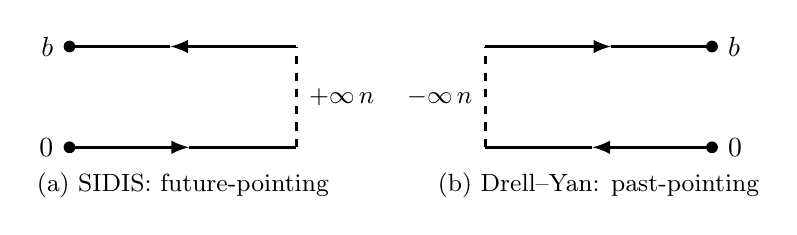
\begin{tikzpicture}[scale=0.8, q/.style={circle, fill=black, inner sep=1.5pt}]
    \begin{scope}[shift={(0,0)}]
      \node[q, label=left:{$0$}] at (0,0) {};
      \node[q, label=left:{$\bvec$}] at (0,1.6) {};
      \draw[very thick, -latex] (0,0) -- (1.9,0);
      \draw[very thick] (1.9,0) -- (3.6,0);
      \draw[very thick, dashed] (3.6,0) -- (3.6,1.6);
      \draw[very thick, -latex] (3.6,1.6) -- (1.6,1.6);
      \draw[very thick] (1.6,1.6) -- (0,1.6);
      \node[right] at (3.65,0.8) {\small $+\infty\,\nminus$};
      \node at (1.8,-0.6) {\small (a) SIDIS: future-pointing};
    \end{scope}
    \begin{scope}[shift={(10.2,0)}]
      \node[q, label=right:{$0$}] at (0,0) {};
      \node[q, label=right:{$\bvec$}] at (0,1.6) {};
      \draw[very thick, -latex] (0,0) -- (-1.9,0);
      \draw[very thick] (-1.9,0) -- (-3.6,0);
      \draw[very thick, dashed] (-3.6,0) -- (-3.6,1.6);
      \draw[very thick, -latex] (-3.6,1.6) -- (-1.6,1.6);
      \draw[very thick] (-1.6,1.6) -- (0,1.6);
      \node[left] at (-3.65,0.8) {\small $-\infty\,\nminus$};
      \node at (-1.8,-0.6) {\small (b) Drell--Yan: past-pointing};
    \end{scope}
  \end{tikzpicture}
  \keymsg{We put this \textbf{staple-shaped link} on the lattice.}
\end{frame}

% Slide 7
\begin{frame}{The $x$-gap on the lattice, and this thesis}
  \begin{columns}[c]
    \begin{column}{0.52\textwidth}
      \begin{itemize}
        \item Light-like separations cannot be placed at a single Euclidean time.
        \item Lorentz-invariant amplitude method with staple links (Musch \emph{et al.} 2012): first lattice Sivers shift and its sign change.
        \item The earlier staple-link Sivers-shift calculations used here sit at $\bvec\tcdot P=0$. Since $\bvec\tcdot P$ is Fourier-conjugate to $x$, they are \textbf{$x$-integrated}.
        \item SIDIS measurements constrain the Sivers function. The combined COMPASS Drell--Yan data are consistent with its predicted sign change; extracting the $x$-shape requires phenomenological fits.
      \end{itemize}
    \end{column}
    \begin{column}{0.46\textwidth}
      \centering
      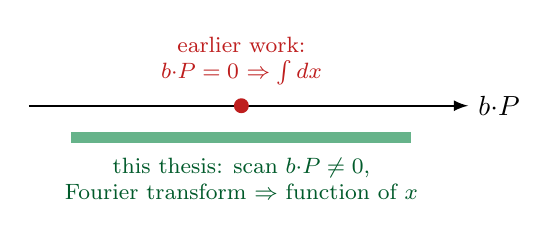
\begin{tikzpicture}[scale=0.9]
        \draw[-latex, thick] (-3,0) -- (3.2,0) node[right] {$\bvec\tcdot P$};
        \fill[badred] (0,0) circle (3pt);
        \node[badred, above, align=center, font=\footnotesize] at (0,0.15) {earlier work:\\$\bvec\tcdot P=0$ $\Rightarrow\int dx$};
        \draw[okgreen, line width=4pt, opacity=0.6] (-2.4,-0.45) -- (2.4,-0.45);
        \node[okgreen!70!black, below, font=\footnotesize, align=center] at (0,-0.6) {this thesis: scan $\bvec\tcdot P\neq0$,\\Fourier transform $\Rightarrow$ function of $x$};
      \end{tikzpicture}
    \end{column}
  \end{columns}
\figsrc{Musch et al., Phys. Rev. D 85, 094510 (2012); COMPASS, Phys. Rev. Lett. 133, 071902 (2024), arXiv:2312.17379.}
\end{frame}
\begin{frame}{The extraction procedure}
  \vspace{2mm}
  \begin{block}{This thesis}
    \begin{enumerate}
      \item Kinematic constraint at $\bvec\tcdot P\neq0$ $\Rightarrow$ off-axis staples, built by interpolation.
      \item Map the data to $(\bvec\tcdot P,\ \bvec^2)$, keeping $|\vect b|\ge 3a$.
      \item Find a model that can be Fourier transformed: a power law, fit to all amplitudes at once.
      \item Fourier transform to $x$, extrapolate to the light-cone limit, test factorization.
    \end{enumerate}
  \end{block}
\figsrc{Thesis, Chs. 5--7: extraction, candidate selection, Fourier transformation and extrapolation.}
\end{frame}

% ===================== QCD (adapted from the 2023 comprehensive-exam slides) =====================
\section{QCD}

% Slide 7
\begin{frame}{Quarks \& gluons}
  \quick
  \centering
  \textbf{Hadrons are made of more fundamental particles: quarks and gluons.}\\[2mm]
  \begin{columns}[c]
    \begin{column}{0.5\textwidth}
      \centering
      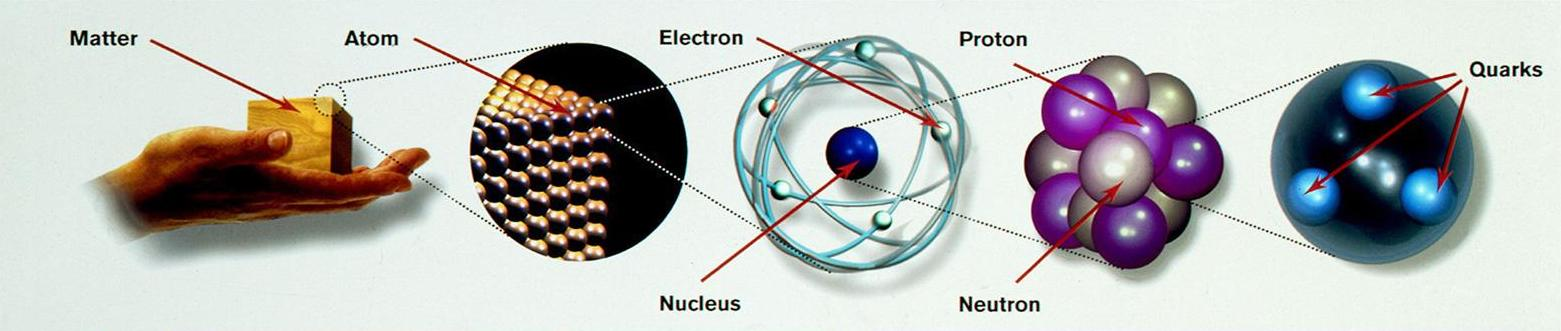
\includegraphics[height=0.55\textheight, width=\linewidth, keepaspectratio]{cmscern.jpeg}\\
      {\scriptsize Atoms are made of electrons and quarks (credit: CMS--CERN)}
    \end{column}
    \begin{column}{0.48\textwidth}
      \centering
      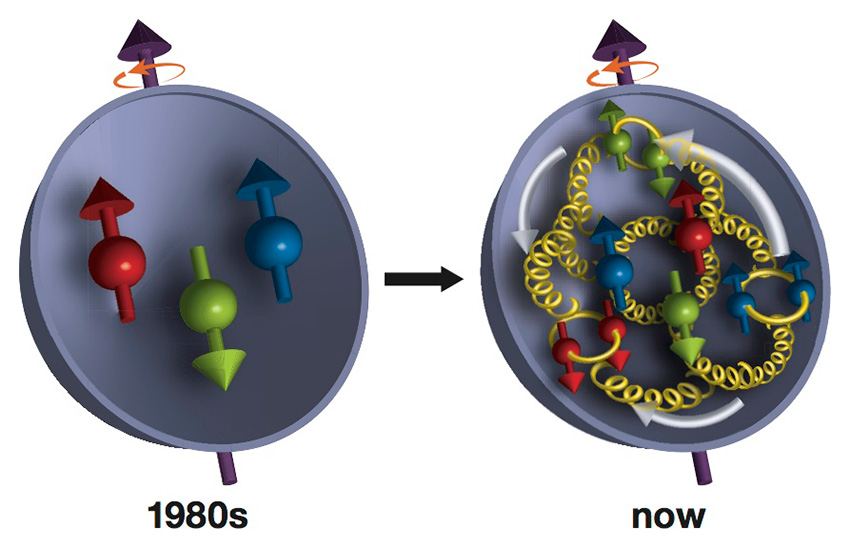
\includegraphics[height=0.55\textheight, width=\linewidth, keepaspectratio]{nucleon-large.jpg}\\
      {\scriptsize Internal structure of hadrons: quarks and gluons (credit: BNL)}
    \end{column}
  \end{columns}
\end{frame}

% Slide 8
\begin{frame}{QCD: Quantum Chromodynamics}
  The QCD Lagrangian density is built from two types of fields:
  \begin{itemize}
    \item spin-$\frac12$ Dirac fields (quarks) $\psi^{i}_{f}$: color $i = 1, 2, 3 = N_c$, flavor $f=u,d,s,c,b,t$;
    \item massless spin-1 vector fields (gluons) $A_{\mu}^{a}$: color $a=1,\ldots,8=N_c^{2}-1$, with local $SU(3)$ color gauge symmetry.
  \end{itemize}
  \[ \boxed{\mathcal{L}_{QCD}=-\frac{1}{4}F^{a}_{\mu\nu}F^{a\,\mu\nu}+\sum_{f}\bar{\psi}_{f}\big(i\gamma^{\mu}D_{\mu}-m_{f}\big)\psi_{f}} \]
  \begin{itemize}
    \item Field strength: $F^a_{\mu\nu}=\partial_{\mu}A^a_{\nu}-\partial_{\nu}A^a_{\mu}+g f^{abc}A^b_{\mu}A^c_{\nu}$
    \item Covariant derivative: $D_{\mu}=\partial_{\mu}-igA^a_{\mu}t^{a}$, \quad $[t^{a},t^{b}]=if^{abc}t^{c}$
    \item Asymptotic freedom at short distances; confinement at hadronic scales $\Rightarrow$ hadron structure is non-perturbative.
  \end{itemize}
\end{frame}

% ===================== Lattice QCD (thesis Ch. 3, with 2023 slides) =====================
\section{Lattice QCD}

% Slide 9
\begin{frame}{Lattice QCD: links, plaquette and the Wilson action}
  \begin{columns}[c]
    \begin{column}{0.42\textwidth}
      \begin{itemize}
        \item Euclidean grid $\Lambda_4$ with spacing $a$. Quarks on sites; gluons as links $U_\mu(x)=e^{iaA_\mu(x)}\in SU(3)$.
        \item Plaquette:
      \end{itemize}
      \[ P_{\mu\nu}(x)=U_{\mu}(x)\,U_{\nu}(x+\hat{\mu})\,U^{\dagger}_{\mu}(x+\hat{\nu})\,U^{\dagger}_{\nu}(x) \]
      \begin{itemize}
        \item Wilson gauge action:
      \end{itemize}
      \[ \begin{aligned} S_{G}&=\frac{2}{g^2}\sum_{x}\sum_{\mu<\nu}\mathrm{Re}\,\Tr\big[1-P_{\mu\nu}(x)\big] \\ &= \frac{a^4}{2g^2}\sum_{x}\sum_{\mu,\nu}\Tr\big[F_{\mu\nu}^2\big]+\mathcal{O}(a^2) \end{aligned} \]
      \begin{itemize}
        \item Quarks: Wilson--clover fermions (removes doublers, $\mathcal O(a)$ improvement).
      \end{itemize}
    \end{column}
    \begin{column}{0.56\textwidth}
      \centering
      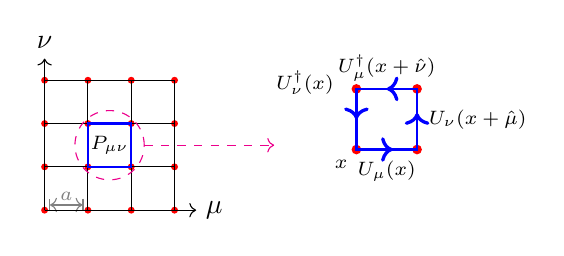
\begin{tikzpicture}[scale=0.55]
        \foreach \x in {0, 1, 2, 3} \foreach \y in {0, 1, 2, 3} \fill[red] (\x, \y) circle (0.08);
        \draw[|<->|, gray] (0.1, 0.12) -- (0.9, 0.12);
        \node at (0.5, 0.32) {\textcolor{gray}{\scriptsize $a$}};
        \foreach \x in {0, 1, 2, 3} \foreach \y in {0, 1, 2} \draw (\x, \y) -- (\x, \y + 1);
        \foreach \x in {0, 1, 2} \foreach \y in {0, 1, 2, 3} \draw (\x, \y) -- (\x + 1, \y);
        \draw[thick, blue] (1, 1) -- (2, 1) -- (2, 2) -- (1, 2) -- cycle;
        \node at (1.5, 1.5) {\scriptsize $P_{\mu\nu}$};
        \draw[->] (0, 0) -- (3.5, 0) node[right] {$\mu$};
        \draw[->] (0, 0) -- (0, 3.5) node[above] {$\nu$};
        \draw[magenta, dashed] (1.5, 1.5) circle (0.8);
        \draw[->, magenta, dashed] (2.3, 1.5) -- (5.3, 1.5);
        \begin{scope}[xshift=5.8cm, scale=1.4]
          \foreach \x in {1, 2} \foreach \y in {1, 2} \fill[red] (\x, \y) circle (0.08);
          \draw[thick, blue] (1, 1) -- (2, 1) -- (2, 2) -- (1, 2) -- cycle;
          \draw[blue,->, line width=1.2pt] (1.5, 1) -- ++(0.1,0);
          \draw[blue,<-, line width=1.2pt] (1.5, 2) -- ++(0.1,0);
          \draw[blue,->, line width=1.2pt] (2, 1.5) -- ++(0,0.1);
          \draw[blue,<-, line width=1.2pt] (1, 1.5) -- ++(0,0.1);
          \node at (0.75, 0.75) {\scriptsize $x$};
          \node at (1.5, 0.65) {\scriptsize $U_{\mu}(x)$};
          \node at (3.0, 1.5) {\scriptsize $U_{\nu}(x+\hat{\mu})$};
          \node at (1.5, 2.35) {\scriptsize $U^{\dagger}_{\mu}(x+\hat{\nu})$};
          \node at (0.15, 2.1) {\scriptsize $U^{\dagger}_{\nu}(x)$};
        \end{scope}
      \end{tikzpicture}
    \end{column}
  \end{columns}
\end{frame}

\begin{frame}{The elementary plaquette in the thesis}
  \centering
  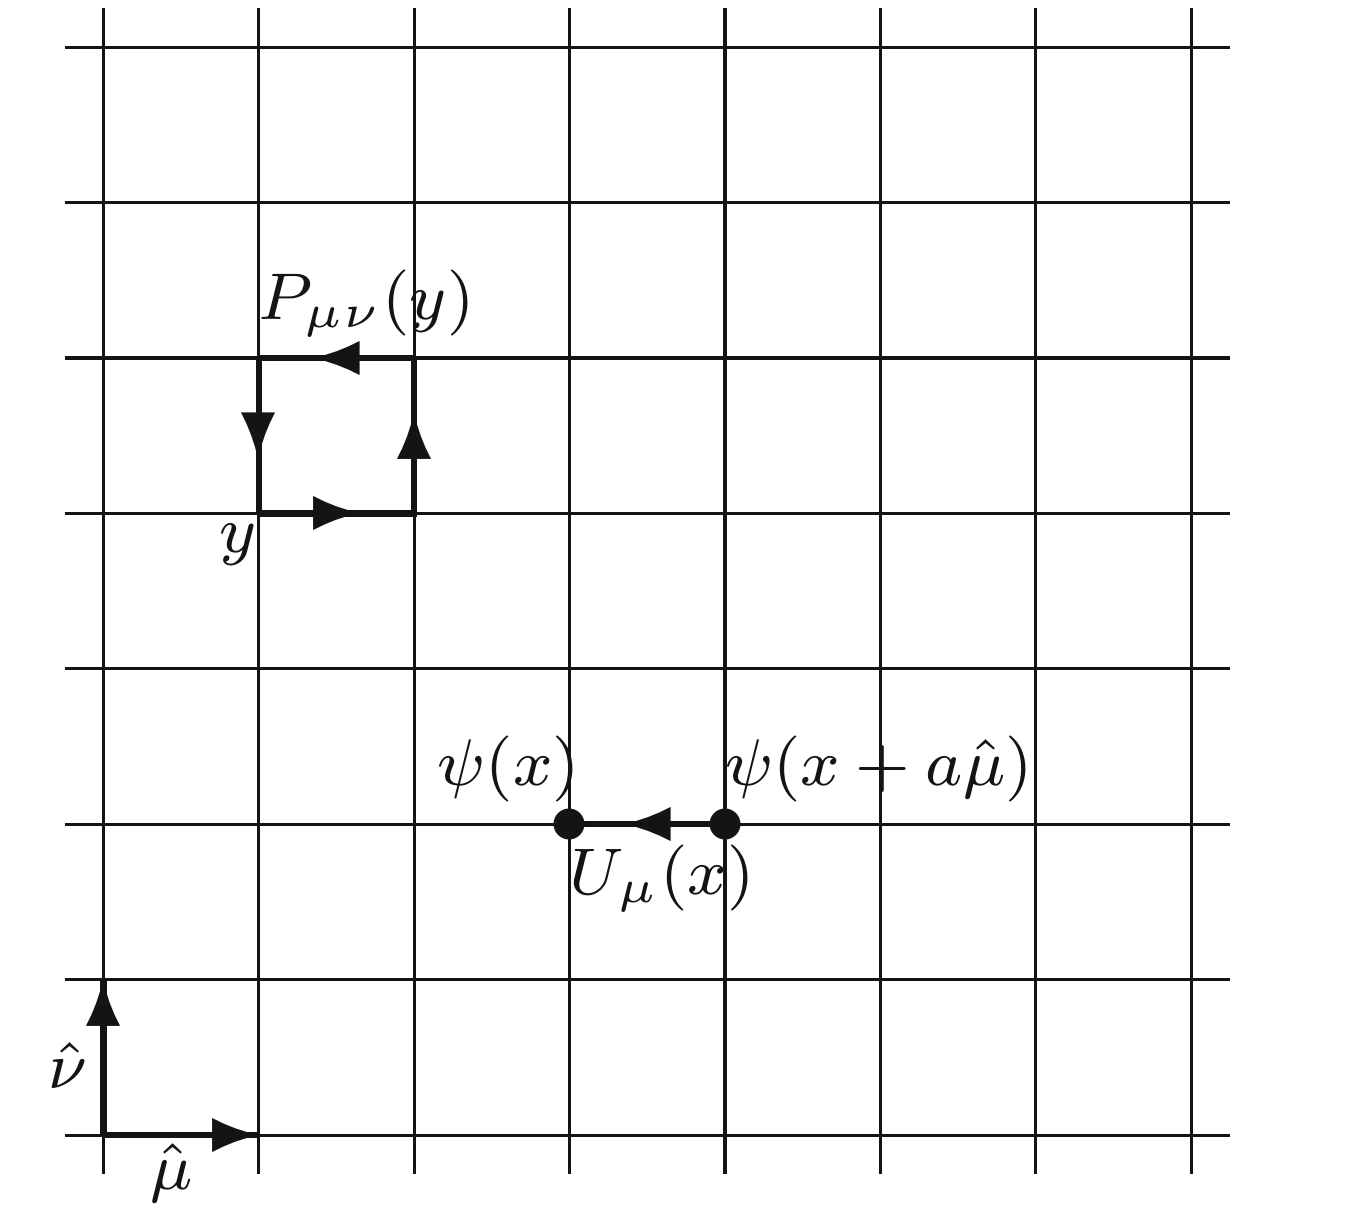
\includegraphics[width=.62\linewidth,height=.65\textheight,keepaspectratio]{LM_fig1_1_plaquette.png}
  \[
   P_{\mu\nu}(x)=U_\mu(x)U_\nu(x+\hat\mu)
                 U_\mu^\dagger(x+\hat\nu)U_\nu^\dagger(x).
  \]
  \figsrc{Thesis, Lattice QCD methodology, original plaquette figure.}
\end{frame}

% Slide 10
\begin{frame}{Path integral, Wick contractions and Monte Carlo}
  \quick
  \begin{columns}[c]
    \begin{column}{0.55\textwidth}
      \begin{itemize}
        \item Observables as Euclidean path integrals:
      \end{itemize}
      \[ \langle \mathcal{O} \rangle =\frac{\int \mathcal{D}[U]\mathcal{D}[\psi]\mathcal{D}[\bar{\psi}]\ \mathcal{O}\ e^{-S_{G}[U]-\bar{\psi}\mathcal{M}[U]\psi}}{\int\mathcal{D}[U]\mathcal{D}[\psi]\mathcal{D}[\bar{\psi}]\ e^{-S_{G}[U]-\bar{\psi}\mathcal{M}[U]\psi}} \]
      \begin{itemize}
        \item Integrating out the Grassmann quark fields gives $\det\mathcal{M}$ and \textbf{Wick contractions}: quark pairs become propagators $S=\mathcal{M}^{-1}$.
        \item Monte Carlo: sample configurations $U_n$ with probability $\propto \prod_f\det\mathcal M_f\; e^{-S_G[U]}$:
      \end{itemize}
      \[ \langle \mathcal O\rangle \approx \frac{1}{N}\sum_{n=1}^{N} \widetilde{\mathcal O}[U_n] \]
    \end{column}
    \begin{column}{0.43\textwidth}
      \centering
      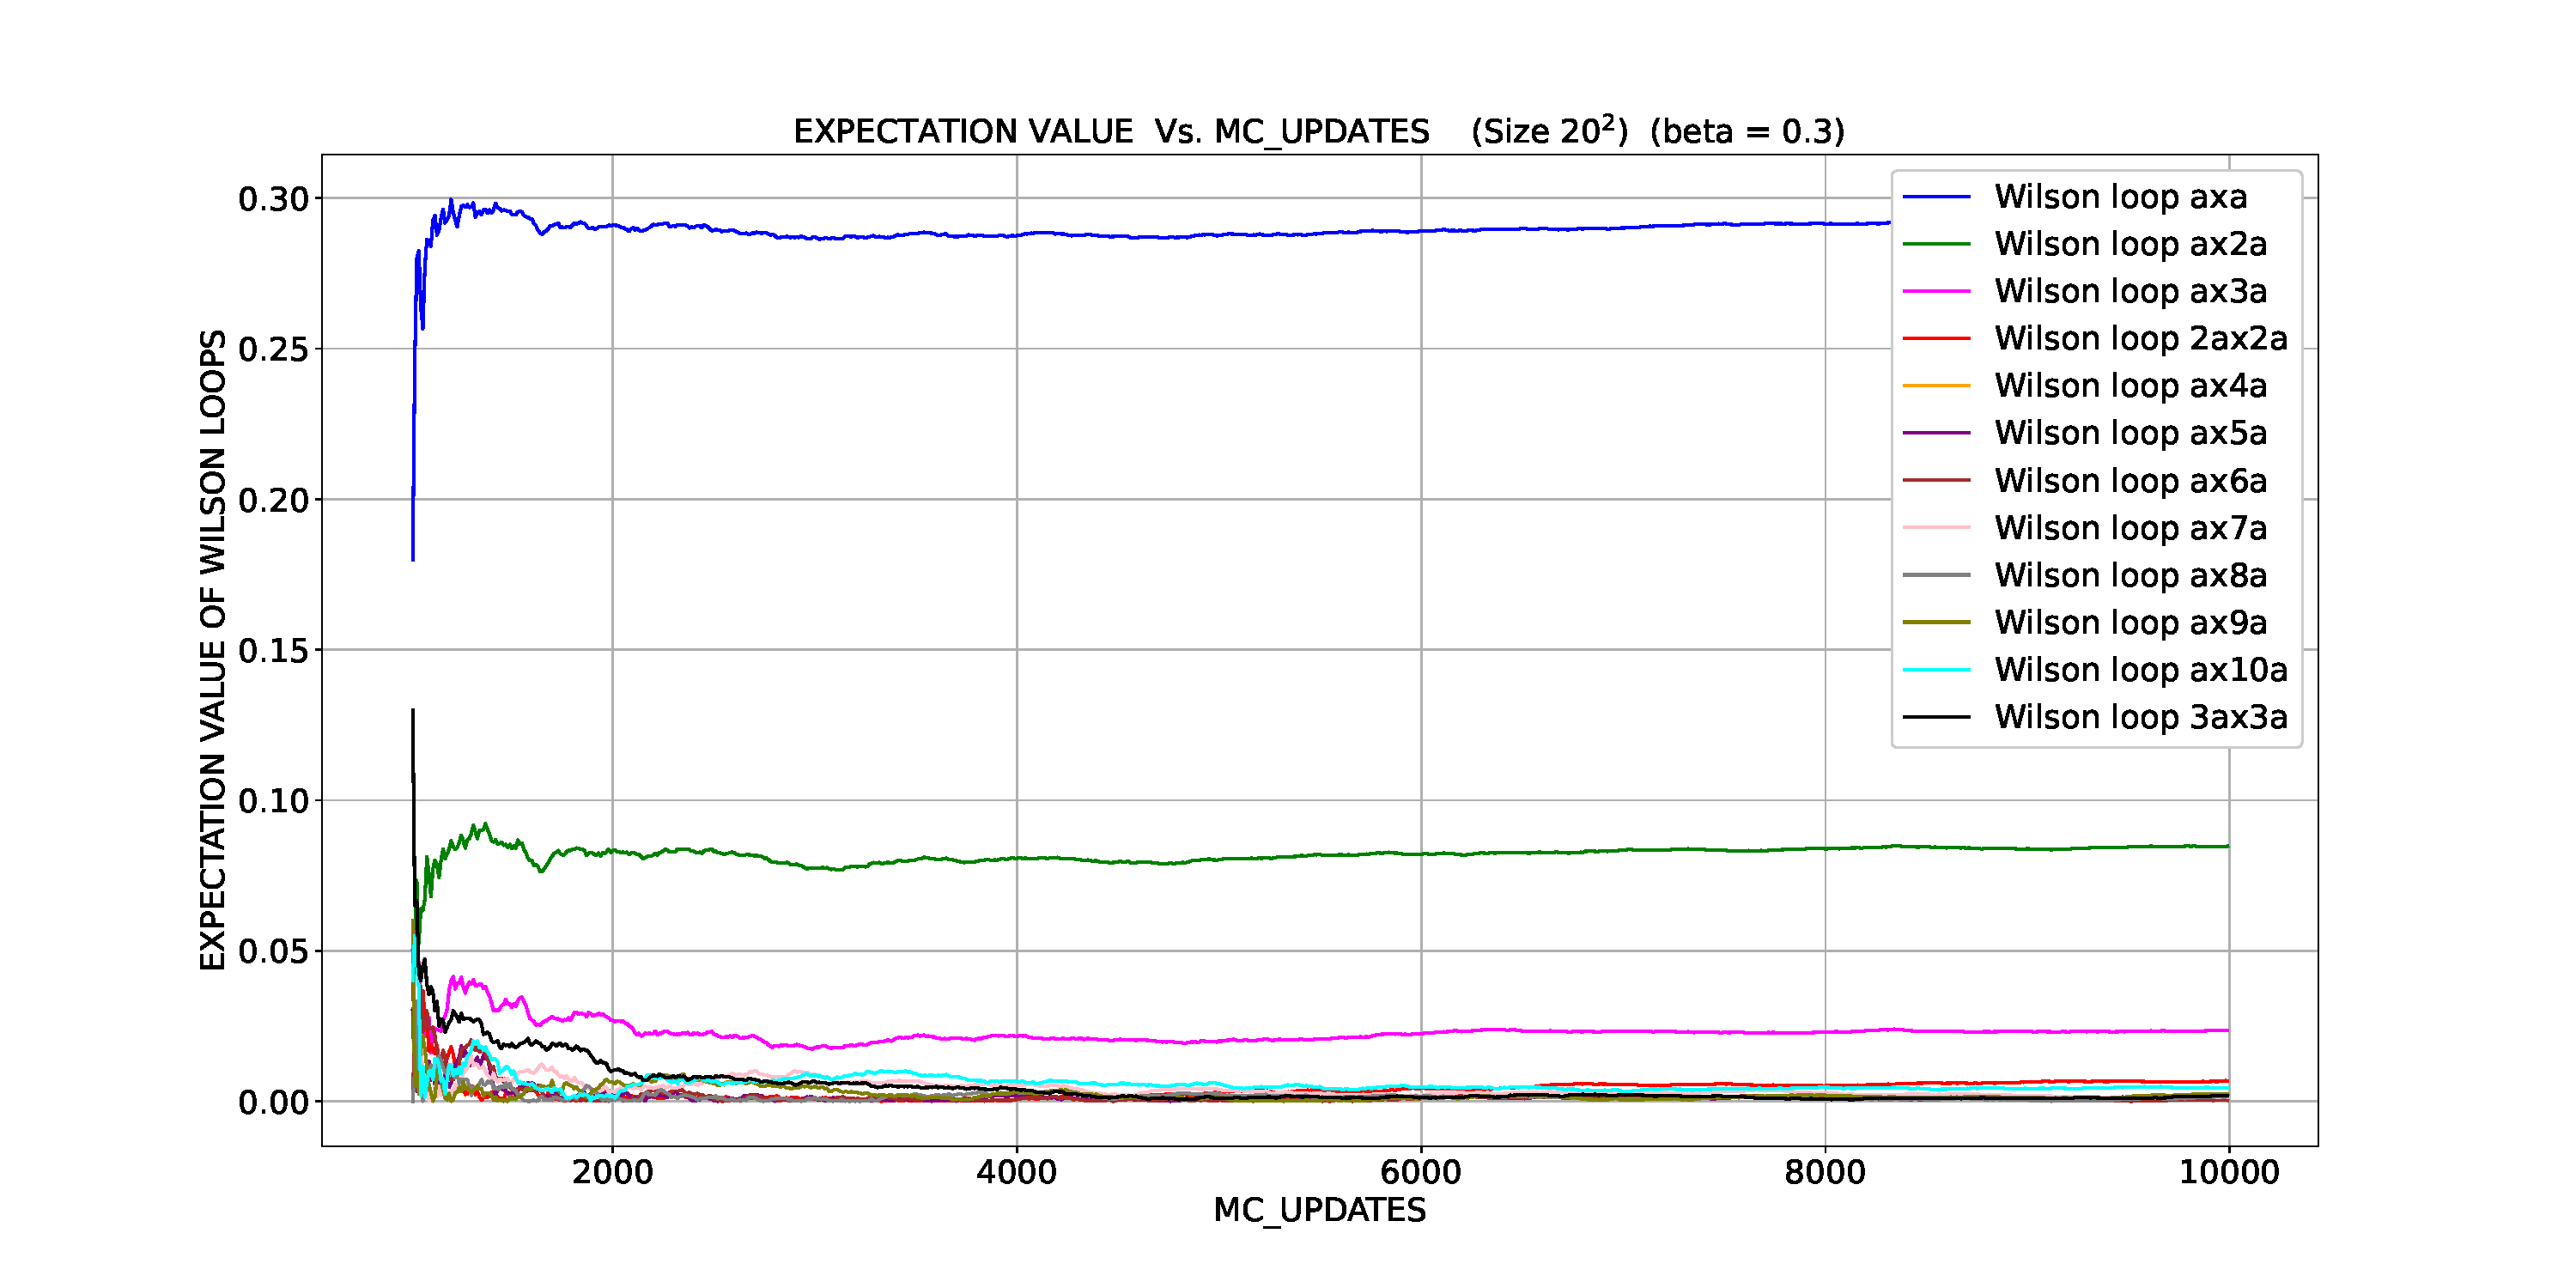
\includegraphics[width=\linewidth]{mcstepsz2.pdf}\\
      {\scriptsize Markov-chain Monte Carlo history (illustration: $\mathbb{Z}_2$ gauge theory in 1+1D)}
    \end{column}
  \end{columns}
\end{frame}

% Slide 11
\begin{frame}{The nucleon two-point function}
  \begin{columns}[c]
    \begin{column}{0.56\textwidth}
      \[ \chi_\alpha(\vect x,t)=\epsilon^{ijk}\,u^i_\alpha\,u^j_\gamma\,[C^{-1}\gamma_5]_{\gamma\delta}\,d^k_\delta \]
      \[ C_{\alpha\beta}(t,\vect p)=a^3\sum_{\vect x}e^{-i\vect p\cdot\vect x}\,\big\langle\chi_\alpha(\vect x,t)\,\bar\chi_\beta(\vect 0,0)\big\rangle \]
      \begin{itemize}
        \item Wick's theorem: two $u$ propagators and one $d$ propagator from the source.
        \item Spectral decomposition, projected with $\Gamma^+=\frac12(1+\gamma_4)$:
      \end{itemize}
      \[ C_{\Gamma^+}(t,\vect p)=|Z(\vect p)|\,\frac{E(\vect p)+m}{E(\vect p)}\,e^{-E(\vect p)t}\,\big[1+\mathcal O\big(e^{-\Delta E\,t}\big)\big] \]
    \end{column}
    \begin{column}{0.42\textwidth}
      \centering
      \begin{tikzpicture}
        \node[inner sep=0] (image) {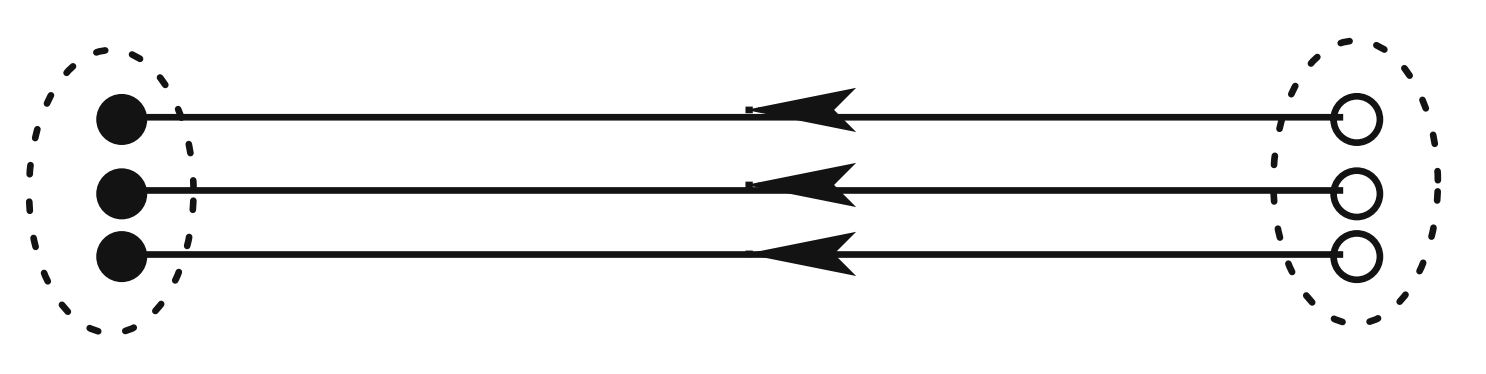
\includegraphics[width=0.85\linewidth]{nucleon_2pt_diagram.png}};
        \node[font=\scriptsize, anchor=south west] at (image.north west) {$(\vect x,t)$};
        \node[font=\scriptsize, anchor=south east] at (image.north east) {$(\vect 0,0)$};
        \node[font=\scriptsize, anchor=north] at (image.south) {$u,\ u,\ d$ propagators $\mathcal{M}^{-1}$};
      \end{tikzpicture}\\[3mm]
      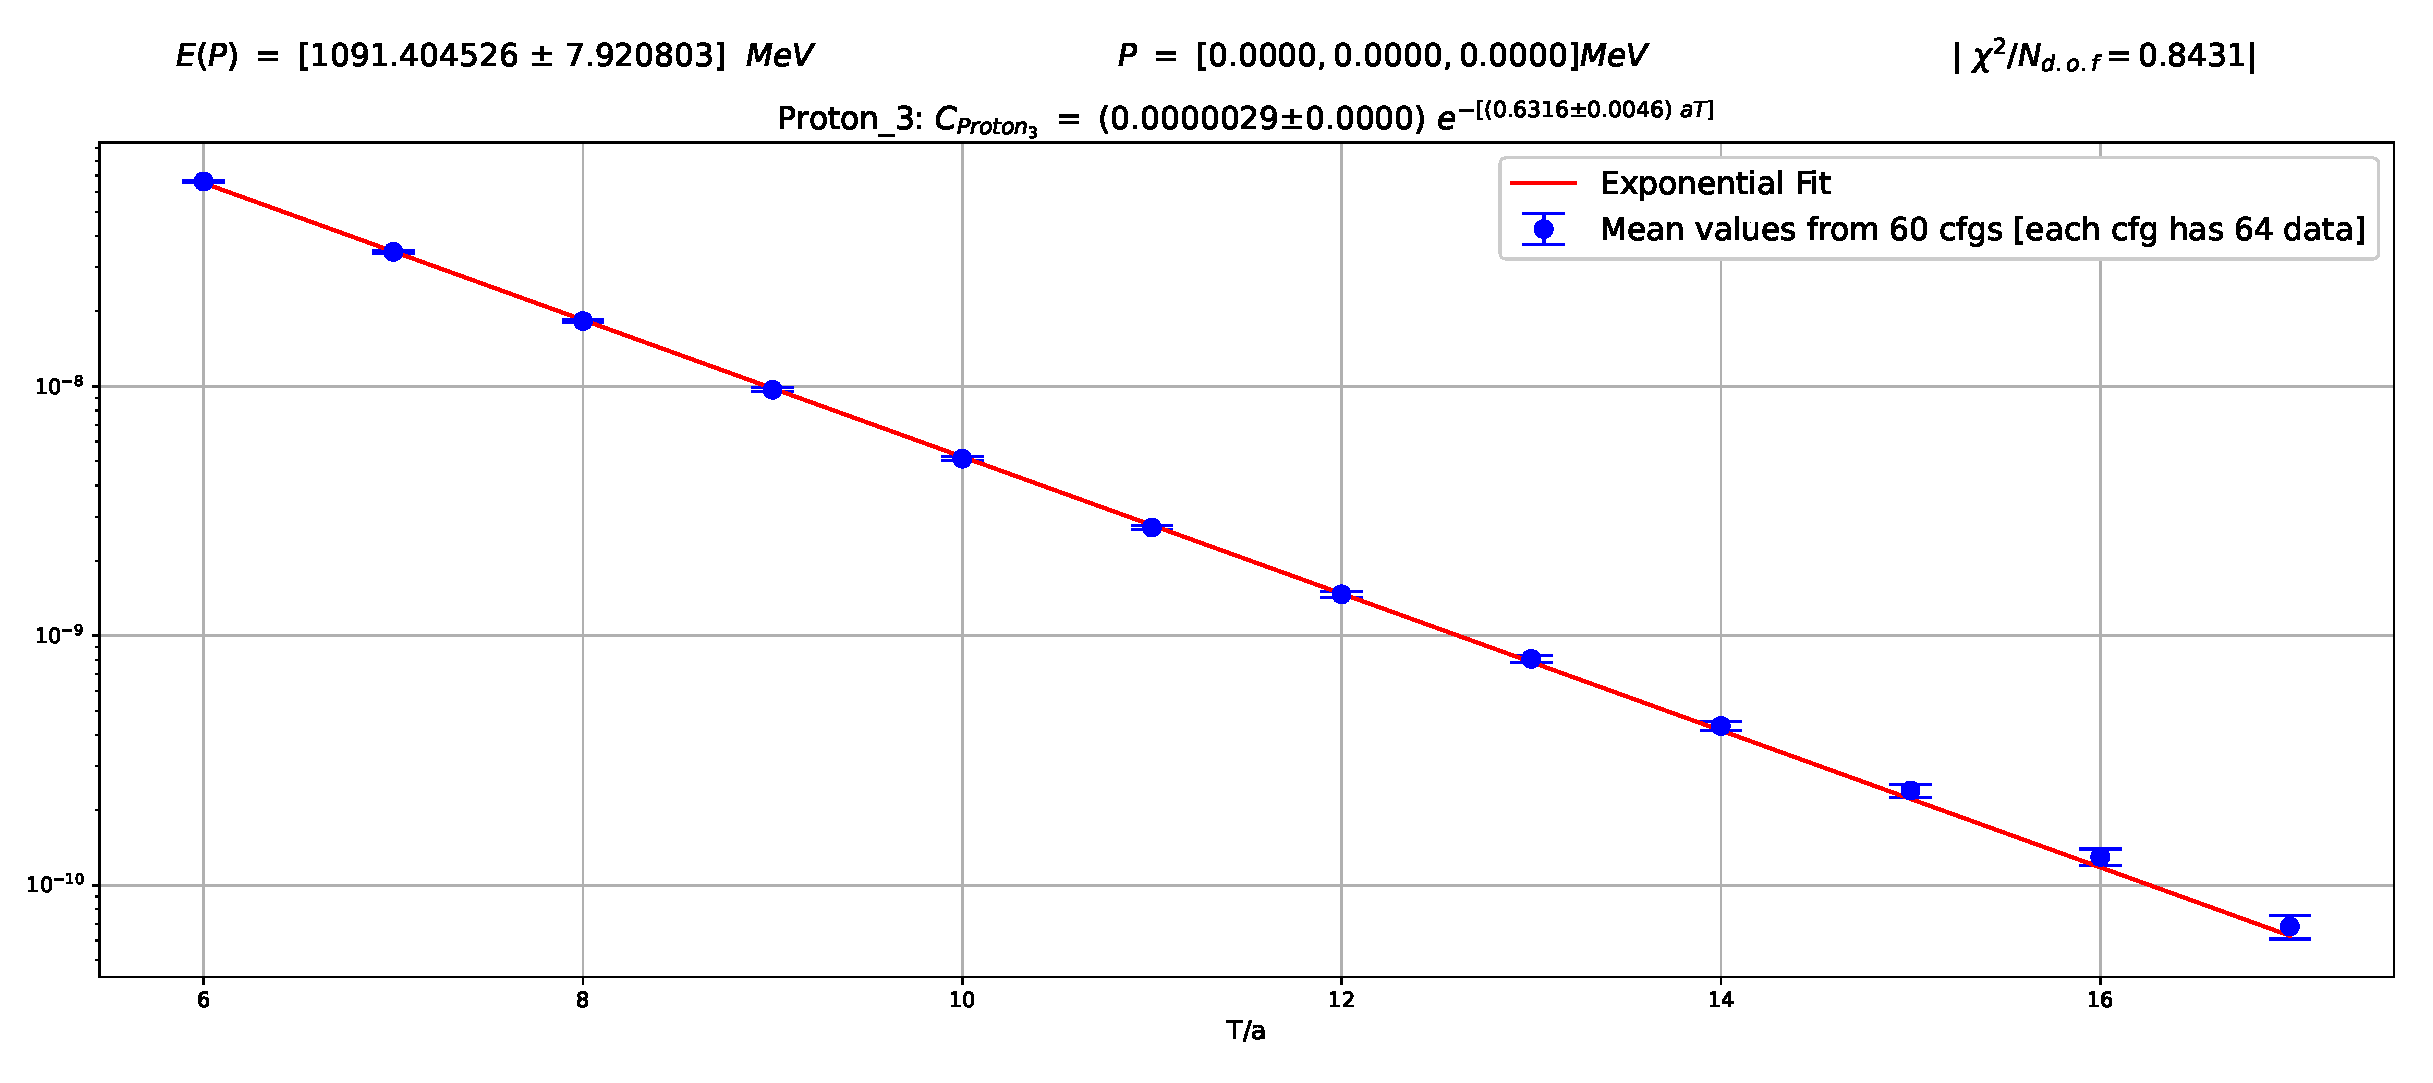
\includegraphics[width=\linewidth]{proton3.eps}\\
      {\scriptsize $C_{\Gamma^+}(t,\vect 0)$ on a different lattice ($32^3\times94$, $a=0.11967$ fm; 2023 study), not the ensemble used in this thesis}
    \end{column}
  \end{columns}
\end{frame}

% Local insertion and complete spectral construction.
\begin{frame}{Nucleon three-point function: source, insertion and sink}
  \small
  \[
  \mathcal O_\Gamma(\vect x_1,\tau)=\bar q(\vect x_1,\tau)\Gamma q(\vect x_1,\tau),
  \qquad 0<\tau<t,\qquad \vect q=\vect p'-\vect p.
  \]
  \begin{align*}
  G(t,\tau;\vect p,\vect p')={}&a^6\sum_{\vect x_2,\vect x_1}
    e^{-i\vect p'\cdot(\vect x_2-\vect x_1)}e^{-i\vect p\cdot\vect x_1}
    \Gamma^{\rm 3pt}_{\beta\alpha}\\
  &\times\big\langle\chi_\alpha(\vect x_2,t)\,
    \mathcal O_\Gamma(\vect x_1,\tau)\,\bar\chi_\beta(\vect 0,0)\big\rangle.
  \end{align*}
  \begin{itemize}
    \item $\bar\chi$ creates nucleon states at the source. The operator acts at $\tau$, and $\chi$ annihilates the states at the sink.
    \item The sink sum projects $\vect p'$. The insertion sum projects the momentum transfer through $e^{i\vect q\cdot\vect x_1}$.
    \item $\Gamma$ specifies the inserted quark bilinear. $\Gamma^{\rm 3pt}$ projects the nucleon spin.
    \item The connected contraction inserts the operator on a nucleon quark line. Disconnected quark loops cancel for $u-d$ in the isospin limit.
  \end{itemize}
  \figsrc{Thesis, Lattice QCD methodology, local three-point functions; Lin (2014), Sec. 3.}
\end{frame}

\begin{frame}{Three-point function: complete spectral sum}
  \small
  With relativistic normalization, insert states on both sides of $\mathcal O$:
  \begin{align*}
  G={}&\sum_{n,n'}\sum_{s,s'}
   \frac{e^{-E_{n'}(\vect p')(t-\tau)}e^{-E_n(\vect p)\tau}}
        {4E_{n'}(\vect p')E_n(\vect p)}\,\Gamma^{\rm 3pt}_{\beta\alpha}\\
  &\times\langle\Omega|\chi_\alpha|N_{n'}(\vect p',s')\rangle
   \langle N_{n'}(\vect p',s')|\mathcal O(\vect q)|N_n(\vect p,s)\rangle\\
  &\times\langle N_n(\vect p,s)|\bar\chi_\beta|\Omega\rangle.
  \end{align*}
  \[
  \langle\Omega|\chi_\alpha|N(\vect p,s)\rangle=\sqrt{Z(\vect p)}\,u_\alpha(\vect p,s),
  \quad
  \langle N'|\mathcal O|N\rangle=\bar u(\vect p',s')\mathcal J u(\vect p,s).
  \]
  \begin{itemize}
    \item $n,n'$ include ground and excited states on the source and sink sides.
    \item Both $\tau$ and $t-\tau$ must be large compared with the inverse excitation gaps for ground-state dominance.
  \end{itemize}
  \figsrc{Thesis, Lattice QCD methodology, spectral decomposition; Lin (2014), Eqs. (3.80)--(3.81).}
\end{frame}

\begin{frame}{Forward matrix element and plateau extraction}
  \small
  For $\vect p'=\vect p$, write $E=E(\vect p)$ and $\Lambda(p)=-i\not\!p+\mN$,
  with Euclidean $p=(\vect p,iE)$.
  \begin{align*}
  G_{00}(t,\tau;\vect p,\vect p)
   &=\frac{|Z(\vect p)|e^{-Et}}{4E^2}
     \Tr[\Gamma^{\rm 3pt}\Lambda(p)\mathcal J\Lambda(p)],\\
  C_{00,\Gamma^+}(t,\vect p)
   &=\frac{|Z(\vect p)|e^{-Et}}{2E}\Tr[\Gamma^+\Lambda(p)],
   \qquad\Gamma^+=\frac{1+\gamma_4}{2}.
  \end{align*}
  \[
  R(t,\tau)=\frac{G(t,\tau)}{C_{\Gamma^+}(t)}
    \xrightarrow{\tau,\,t-\tau\to\infty}
  \frac{\Tr[\Gamma^{\rm 3pt}\Lambda(p)\mathcal J\Lambda(p)]}
       {2E\,\Tr[\Gamma^+\Lambda(p)]}.
  \]
  \begin{itemize}
    \item $G_{00}$ and $C_{00}$ denote the ground-state terms. The overlaps and $e^{-Et}$ cancel in their ratio.
    \item The measured ratio approaches a $\tau$-independent plateau. Finite separations retain excited-state contamination.
    \item A sequential-source inversion fixes the sink time, momentum and spin projector while allowing insertion positions to vary.
  \end{itemize}
  \figsrc{Thesis, Lattice QCD methodology, ratio and sequential propagators; Lin (2014).}
\end{frame}

\begin{frame}{Three-point function: skeleton diagram}
  \centering
  \begin{tikzpicture}[>=Stealth,scale=1.0,
      qline/.style={thick,postaction={decorate},decoration={markings,mark=at position 0.55 with {\arrow{Stealth}}}}]
    % time axis
    \draw[->,gray] (-0.6,-2.6) -- (10.2,-2.6) node[right,gray] {$t$};
    \foreach \x/\l in {0/{0 (source)},4.8/{\tau},9.6/{t (sink)}} \draw[gray] (\x,-2.5)--(\x,-2.7) node[below,font=\small] {$\l$};
    % source and sink blobs
    \fill[blue!25,draw=blue!60!black,thick] (0,0) ellipse (0.45 and 1.5);
    \fill[blue!25,draw=blue!60!black,thick] (9.6,0) ellipse (0.45 and 1.5);
    \node[blue!60!black] at (0,-1.9) {$\bar\chi_\beta(\vect 0,0)$};
    \node[blue!60!black] at (9.6,-1.9) {$\chi_\alpha(\vect x_2,t)$};
    % spectator quarks
    \draw[qline] (0.4,0.7) -- (9.2,0.7);
    \draw[qline] (0.4,0.0) -- (9.2,0.0);
    \node[font=\small] at (4.8,1.05) {spectator quarks};
    % active quark through the operator
    \draw[qline,red!70!black] (0.4,-0.7) -- (4.5,-0.7);
    \draw[qline,red!70!black] (5.1,-0.7) -- (9.2,-0.7);
    \node[fill=red!15,draw=red!70!black,thick,circle,inner sep=3pt] at (4.8,-0.7) {$\mathcal O_\Gamma$};
    \node[red!70!black,font=\small] at (2.4,-1.15) {propagator $S(\vect x_1,\tau;0)$};
    \node[red!70!black,font=\small] at (7.2,-1.15) {sequential propagator};
    \draw[gray,dashed] (4.8,-2.5)--(4.8,1.3);
    \node[font=\small] at (4.8,1.6) {$\mathcal O(\vect x_1,\tau)=\bar q\,\Gamma\,q$};
  \end{tikzpicture}
  \figsrc{Existing schematic of the connected contraction; topology as in thesis, Lattice QCD methodology (Lin, 2014).}
  \begin{itemize}\footnotesize
    \item Connected topology: one quark line (red) carries the operator insertion. Sum over operator position $\vect x_1$ at fixed $\tau$ projects the momentum transfer; the sink sum projects $\vect p'$.
    \item For the TMD operator the single vertex is replaced by the non-local $\bar q(0)\,\Gamma\,\mathcal U\,q(\bvec)$ with a staple gauge link (next slide).
  \end{itemize}
\end{frame}

% Slide 13
\begin{frame}{Non-local staple three-point function: what we compute}
  \begin{columns}[c]
    \begin{column}{0.55\textwidth}
      \begin{itemize}
        \item TMD operator: $\bar q(0)\,\Gamma\,\mathcal U[0,\eta v,\eta v+\bvec,\bvec]\,q(\bvec)$: quark separation $\bvec$, staple direction $v$, staple length $\eta|v|$. Both purely spatial, so the operator sits in one time slice.
        \item On the lattice the staple is a step-wise path $\mathcal C^{\rm lat}$:
      \end{itemize}
      \[ \begin{aligned} C^{\rm 3pt}_{\Gamma}(\tau,\vect P;\mathcal C^{\rm lat})=\frac{1}{\hat L^3}\sum_{z}\Gamma^{\rm 3pt}_{\beta\alpha}\big\langle&\chi_\alpha(t_{\rm snk},\vect P)\,O^{\rm lat}_{\Gamma}(\mathcal C^{\rm lat};z,\tau)\\ &\times\bar\chi_\beta(t_{\rm src},\vect P)\big\rangle \end{aligned} \]
      \[ R_{\Gamma}(\vect P;\mathcal C^{\rm lat})\equiv\mathrm{plateau}\left[\frac{C^{\rm 3pt}_{\Gamma}(\tau,\vect P;\mathcal C^{\rm lat})}{C^{\rm 2pt}(t_{\rm snk}-t_{\rm src},\vect P)}\right] \]
      \begin{itemize}
        \item Inputs: $R_{\Gamma(n)}$ for $\Gamma=\gamma_1,\gamma_2,\gamma_3,\gamma_4$ (isovector $u-d$).
      \end{itemize}
      {\scriptsize Ensemble: $n_f=2+1$ clover, $32^3\times96$, $a=0.11403$ fm, $\mN a=0.6228(28)$ ($\mN=1077.8(48)$ MeV).}
    \end{column}
    \begin{column}{0.43\textwidth}
      \centering
      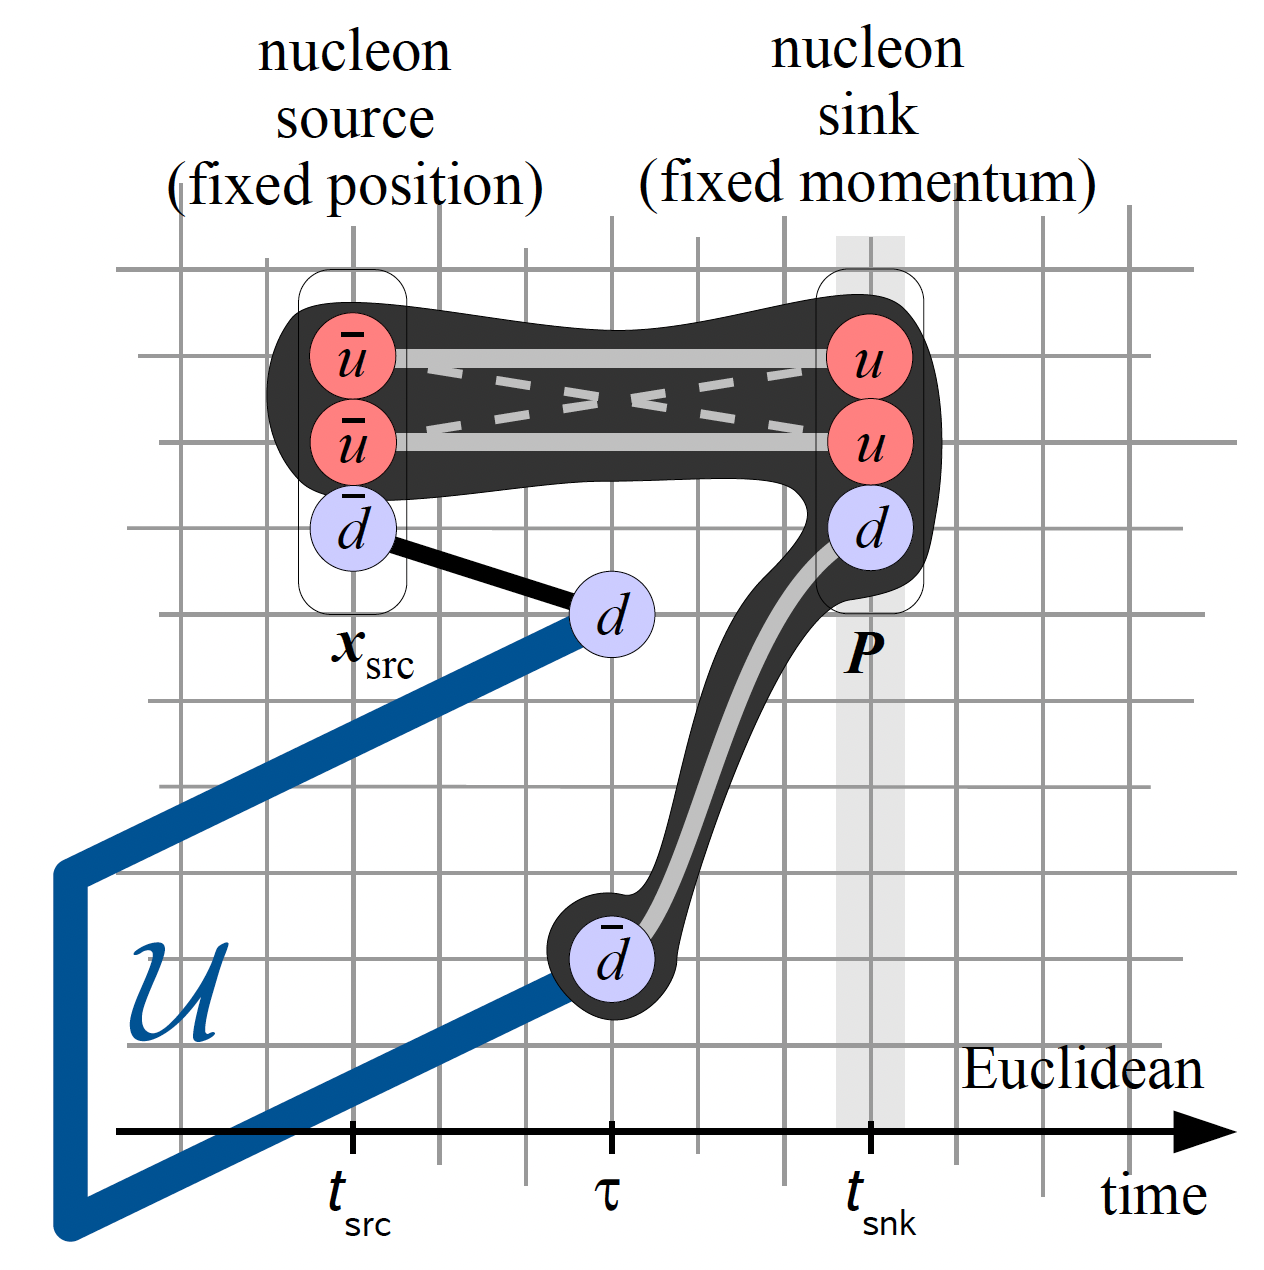
\includegraphics[width=0.9\linewidth]{lattice_3pt_staple_Engelhardt.png}\\
      \figsrc{Figure credit: M.~Engelhardt (NMSU)}
    \end{column}
  \end{columns}
\end{frame}

% ===================== TMD correlator for lattice calculations (thesis Ch. 4) =====================
\section{TMD correlator}

% Slide 14
\begin{frame}{Definition of TMDs}
  \begin{itemize}
    \item Nucleon with $P^+\gg\mN$, $\vprp P=0$: $x=k^+/P^+$ and $\vprp k$ are boost invariant along $z$.
    \item Gauge-invariant bilocal operator, divided by the soft factor $\widetilde{\softf}$ (rapidity divergences). Wilson-line geometry, rapidity-regulator and renormalization-scale arguments are held fixed and suppressed below:
  \end{itemize}
  \[ \Phi^{[\Gamma]}(\kei,P,S)\equiv\int \frac{d^4 \bvec}{(2\pi)^4}\, e^{i \kei\cdot \bvec}\,
     \frac{\overbrace{\tfrac{1}{2}\, \bra{P,S}\ \bar{q}(0)\, \Gamma\ \WlineC{\mathcal{C}_\bvec}\ q(\bvec)\ \ket{P,S}}^{\textstyle \equiv\ \widetilde \Phi_\unsub^{[\Gamma]}(\bvec,P,S)}}{\widetilde{\softf}(\bvec^2)} \]
  \begin{itemize}
    \item Integrating over $k^-$ sets $\bvec^+=0$:
  \end{itemize}
  \[ \Phi^{[\Gamma]}(x,\vprp{k};P,S)=\int \frac{d^2 \vprp{\bvec}}{(2\pi)^2} \int \frac{d (\bvec \tcdot P)}{(2\pi) P^+}\ e^{i x (\bvec \tcdot P) - i\vprp{\bvec} \tcdot \vprp{\kei}}\,\frac{\widetilde \Phi_\unsub^{[\Gamma]}}{\widetilde{\softf}}\Big|_{\bvec^+=0} \]
  \keymsg{$x \leftrightarrow \bvec \tcdot P$ \ and \ $\vprp{k} \leftrightarrow \vprp{b}$ are Fourier pairs. \qquad
  $\Phi^{[\gamma^+]} = f_1 - \dfrac{\myeps_{ij}\, k_{i}\, S_{j}}{\mN}\ f_{1T}^\prp$}
\end{frame}

% Slide 15
\begin{frame}{TMDs in Fourier space}
  \begin{itemize}
    \item The lattice computes $\bvec$-space matrix elements, so we state results for $\vprp b$-dependent TMDs:
  \end{itemize}
  \[ \tilde f(x, \vprp{\bvec}^2) \equiv \int  d^2 \vprp{\kei} \, e^{i \vprp{\bvec} \cdot \vprp{\kei} }\, f(x, \vprp{\kei}^2)
     = 2\pi \int d|\vprp{\kei}|\, |\vprp{\kei}|\ J_0(|\vprp{\bvec}||\vprp{\kei}|)\  f(x, \vprp{\kei}^2) \]
  \[ \tilde f^{(n)}(x, \vprp{\bvec}^2) \equiv n!\left( -\frac{2}{\mN^2}\partial_{\vprp{\bvec}^2} \right)^n \tilde f(x, \vprp{\bvec}^2)
     \ \xrightarrow{\ |\vprp b|\to0\ }\ \int  d^2 \vprp{\kei} \left( \frac{\vprp{\kei}^2}{2 \mN^2 }\right)^n  f(x, \vprp{\kei}^2) \]
  \begin{itemize}
    \item $\tilde f_1^{(0)}$: unpolarized; \ $\tilde f_{1T}^{\perp(1)}$: first $\vprp k$-moment of the Sivers function.
    \item $f_{1T}^{\perp(1)}(x)$ diverges without extra regularization (high-$\vprp k$ tail), so we \textbf{stay at finite $|\vprp b|$}.
    \item Finite $|\vprp b|$ provides Bessel weighting. The correlator still requires ultraviolet and rapidity renormalization. We reach $x$ through $\bvec\tcdot P$.
  \end{itemize}
\end{frame}

% Slide 16
\begin{frame}{Link geometry}
  \begin{columns}[c]
    \begin{column}{0.55\textwidth}
      \begin{itemize}
        \item Staple-shaped link $\mathcal U[0,\eta v,\eta v+\bvec,\bvec]$: legs along $v$ of length $\eta|v|$, joined at the far end.
        \item Large staple extent: SIDIS for $\eta v\tcdot P\to+\infty$ and Drell--Yan for $\eta v\tcdot P\to-\infty$.
        \item On the lattice $\bvec$ and $v$ are purely spatial (space-like). Collins--Soper parameter:
      \end{itemize}
      \[ \zetahat \equiv \frac{\zeta}{2\mN}=\frac{v \cdot P}{\sqrt{|v^2|}\, \sqrt{P^2}} = \sinh(y_P - y_v) \]
      \begin{itemize}
        \item Light-like $v$ (the TMD limit) $\Leftrightarrow$ $\zetahat\to\infty$.
      \end{itemize}
    \end{column}
    \begin{column}{0.43\textwidth}
      \centering
      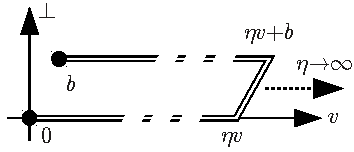
\includegraphics[width=\linewidth]{StapleLink2.pdf}
    \end{column}
  \end{columns}
\end{frame}

% Slide 17
\begin{frame}{Symmetry constraints: the amplitudes are complex}
  \begin{itemize}
    \item The correlator is decomposed into Lorentz-invariant amplitudes ($A_i$, $B_i$ in momentum space; $\tAmp_i$, $\tBmp_i$ in $\bvec$-space; next slide). Lorentz, parity, time reversal and Hermiticity constrain it; in momentum space Hermiticity makes $A_i$, $B_i$ \textbf{real}.
    \item In $\bvec$-space ($\kei\to -i\mN^2\bvec$), Hermitian conjugation gives
  \end{itemize}
  \[ \big[\widetilde{\Phi}^{[\GammaOp]}_{\unsub}(\bvec,P,S;v)\big]^* = \widetilde{\Phi}^{[\gamma^0 \GammaOp^\dagger \gamma^0]}_{\unsub}(-\bvec,P,S;v) \]
  \[ \Rightarrow\quad \big[\tAmp_i(\bvec^2,\bvec \tcdot P, \tfrac{v \tcdot \bvec}{v \tcdot P}, \zeta^{-2})\big]^* = \tAmp_i(\bvec^2,-\bvec \tcdot P, -\tfrac{v \tcdot \bvec}{v \tcdot P}, \zeta^{-2}) \]
  \keymsg{$\tAmp_i=\tAmp_i^{\text{Re}}+i\tAmp_i^{\text{Im}}$ \ are complex, with \ $\tAmp_i^{\text{Re}}$: even in $\bvec$, \quad $\tAmp_i^{\text{Im}}$: odd in $\bvec$ \quad (same for $\tBmp_i$)}
\end{frame}

% Full vector decomposition, with no suppressed tensor structures.
\begin{frame}{Complete vector-correlator decomposition}
  \small
  \begin{align*}
  \frac12\widetilde\Phi_{\unsub}^{[\gamma^\mu]}
   ={}&P^\mu\tAmp_2-i\mN^2 b^\mu\tAmp_3
       -i\mN\epsilon^{\mu\nu\alpha\beta}P_\nu b_\alpha S_\beta\tAmp_{12}\\
   &+\frac{\mN^2}{v\cdot P}v^\mu\tBmp_1
       +\frac{\mN}{v\cdot P}\epsilon^{\mu\nu\alpha\beta}P_\nu v_\alpha S_\beta\tBmp_7\\
   &-\frac{i\mN^3}{v\cdot P}\epsilon^{\mu\nu\alpha\beta}b_\nu v_\alpha S_\beta\tBmp_8\\
   &-\frac{\mN^3}{v\cdot P}(b\cdot S)\epsilon^{\mu\nu\alpha\beta}P_\nu b_\alpha v_\beta\tBmp_9\\
   &-\frac{i\mN^3}{(v\cdot P)^2}(v\cdot S)\epsilon^{\mu\nu\alpha\beta}P_\nu b_\alpha v_\beta\tBmp_{10}.
  \end{align*}
  \begin{itemize}
    \item All eight allowed structures of this vector channel are retained.
    \item Each amplitude is a function of
    $\big(b\cdot b,\ b\cdot P,\ (v\cdot b)/(v\cdot P),\ -1/(\mN\zetahat)^2,\ \eta v\cdot P\big)$.
    \item Here $b\cdot b$ is the Minkowski square. A spatial component $b^2$ later denotes the second component, not this invariant.
  \end{itemize}
  \figsrc{Thesis, TMD framework, vector parametrization; Musch et al., Phys. Rev. D 85, 094510 (2012).}
\end{frame}

\begin{frame}{The two amplitude combinations entering the Sivers shift}
  In the TMD frame, $b^+=0$ and $\vprp v=\vprp P=0$ fix the third invariant:
  \[
  \frac{v\cdot b}{v\cdot P}=(b\cdot P)\frac{R(\zetahat^2)}{\mN^2},
  \qquad R(\zetahat^2)=1-\sqrt{1+\zetahat^{-2}}.
  \]
  The $\gamma^+$ projection becomes
  \[
  \frac{1}{2P^+}\widetilde\Phi_{\unsub}^{[\gamma^+]}
  =\tAmp_{2B}+i\mN\epsilon_{ij}\vect b_i\vect S_j\tAmp_{12B}.
  \]
  \[
    \boxed{\tAmp_{2B}=\tAmp_2+R(\zetahat^2)\tBmp_1},
    \qquad
    \boxed{\tAmp_{12B}=\tAmp_{12}-R(\zetahat^2)\tBmp_8}.
  \]
  \begin{itemize}
    \item These combinations follow from the full vector decomposition.
    \item We determine them from the four Euclidean vector channels, after path averaging and interpolation.
  \end{itemize}
  \figsrc{Thesis, TMD framework, TMD-frame reduction; Musch et al. (2012).}
\end{frame}

% Slide 19
\begin{frame}{Generalized Sivers shift from amplitudes}
  \begin{itemize}
    \item Average $k_y$ of unpolarized quarks in a nucleon polarized along $\hat x$ ($T$: transversely polarized nucleon, $U$: unpolarized quark), generalized to finite $|\vprp b|$:
  \end{itemize}
  \begin{block}{}
  \[ \langle k_y\rangle_{TU}(\vprp{b}^2;\zetahat,\eta v\tcdot P) \equiv \mN\,\frac{\tilde f_{1T}^{\perp[1](1)}(\vprp{b}^2)}{\tilde f_1^{[1](0)}(\vprp{b}^2)}
     = -\mN\,\frac{\tAmp_{12B}(-\vprp{b}^2,0,0,-1/(\mN\zetahat)^2,\eta v\tcdot P)}{\tAmp_{2B}(-\vprp{b}^2,0,0,-1/(\mN\zetahat)^2,\eta v\tcdot P)} \]
  \end{block}
  \begin{itemize}
    \item Under $\Gamma$-independent multiplicative renormalization, the soft factor and $Z$ cancel in this ratio at fixed geometry $(\bvec,P,\eta v)$.
    \item At $\bvec\tcdot P=0$ this ratio is \textbf{integrated over $x$}: the quantity computed in earlier lattice work.
  \end{itemize}
  \keymsg{This thesis: keep $\bvec\tcdot P\neq0$ and Fourier transform, to get the shift \textbf{as a function of $x$}.}
\end{frame}

% ===================== Lattice data & extracting the x-dependence (thesis Ch. 5) =====================
\section{Lattice data}

\begin{frame}{The $x$-dependent Sivers shift}
  Write $\nu=b\cdot P$ and keep $s=-b_\mu b^\mu$, $\zetahat$, and $\eta v\cdot P$ fixed:
  \[
    \tAmp_{iB}^{[x]}(s,x,\zetahat,\eta v\cdot P)
    =\int_{-\infty}^{\infty}\frac{d\nu}{2\pi}\,
      e^{ix\nu}\tAmp_{iB}(s,\nu,\zetahat,\eta v\cdot P).
  \]
  \[
    \langle k_y\rangle_{TU}(s,x,\zetahat,\eta v\cdot P)
    =m_N\frac{\tilde f_{1T}^{\perp(1)}(s,x,\zetahat,\eta v\cdot P)}
                  {\tilde f_1^{(0)}(s,x,\zetahat,\eta v\cdot P)}
    =-m_N\frac{\tAmp_{12B}^{[x]}}{\tAmp_{2B}^{[x]}}.
  \]
  \begin{itemize}
    \item In the lattice frame, $s=b_L^2+b_T^2$. In the TMD frame with $b^+=0$, $s=|\vect b_{T,\mathrm{TMD}}|^2$.
    \item The Fourier transform varies $\nu$ at fixed $s$; it is not a transform at fixed lattice $b_T$.
    \item The common soft factor cancels at fixed geometry under the multiplicative-renormalization assumption used in the thesis.
  \end{itemize}
  \figsrc{Thesis, Ch. 5: Sivers shift as a function of momentum fraction $x$.}
\end{frame}

\begin{frame}{Cosine and sine transforms of the complex amplitudes}
  At fixed $(s,\zetahat,\eta v\cdot P)$, define the real quantities
  \begin{align*}
    E_i(x)&=\int_{-\infty}^{\infty}\frac{d\nu}{2\pi}\cos(x\nu)\tAmp_{iB}^{\mathrm{Re}}(\nu),\\
    O_i(x)&=\int_{-\infty}^{\infty}\frac{d\nu}{2\pi}\sin(x\nu)\tAmp_{iB}^{\mathrm{Im}}(\nu).
  \end{align*}
  \[
    \tAmp_{iB}^{[x]}=E_i-O_i+
    i\int_{-\infty}^{\infty}\frac{d\nu}{2\pi}
       [\sin(x\nu)\tAmp_{iB}^{\mathrm{Re}}(\nu)
        +\cos(x\nu)\tAmp_{iB}^{\mathrm{Im}}(\nu)].
  \]
  \begin{itemize}
    \item $\tAmp^{\mathrm{Re}}$ is even and $\tAmp^{\mathrm{Im}}$ odd in $\nu$. The remaining imaginary integral vanishes by parity, when the integrals exist.
    \item Therefore $\tAmp_{iB}^{[x]}=E_i-O_i$ is real. The thesis labels these two real transforms $\tAmp_{iB}^{[x]\mathrm{Re}}$ and $\tAmp_{iB}^{[x]\mathrm{Im}}$.
  \end{itemize}
  \[ \langle k_y\rangle_{TU}=-m_N\frac{E_{12}-O_{12}}{E_2-O_2}. \]
  \figsrc{Thesis, Ch. 5: Fourier decomposition; all transform signs follow $e^{+ix\nu}$.}
\end{frame}

% Slide 21
\begin{frame}{The Collins--Soper parameter $\zetahat$}
  \quick
  \begin{columns}[c]
    \begin{column}{0.55\textwidth}
      \[ \zetahat = \frac{v \cdot P}{\sqrt{|v^2|}\, \sqrt{P^2}} \]
      \begin{itemize}
        \item On the lattice the staple direction $v$ must be space-like ($v^2<0$), purely spatial ($v_0=0$).
        \item The physical TMD limit needs $\zetahat\to\infty$ (light-like $v$).
        \item Larger $\zetahat$ requires larger nucleon momentum $\vect P$.
        \item We track the Sivers shift over several $\zetahat$ and \textbf{extrapolate}.
      \end{itemize}
    \end{column}
    \begin{column}{0.43\textwidth}
      \centering
      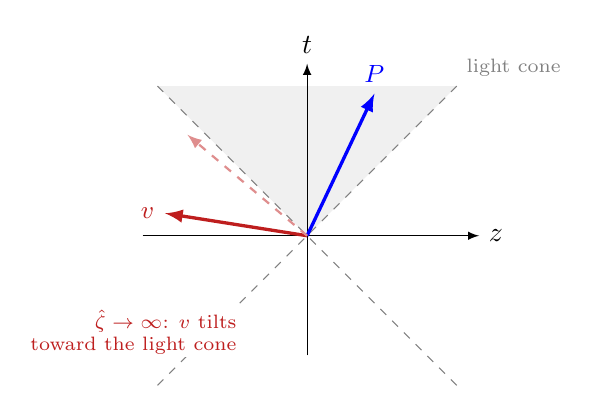
\begin{tikzpicture}[scale=0.95]
        \fill[gray!12] (0,0) -- (2,2) -- (-2,2) -- cycle;
        \draw[gray, dashed] (-2,-2) -- (2,2) node[above right, font=\scriptsize] {light cone};
        \draw[gray, dashed] (2,-2) -- (-2,2);
        \draw[-latex] (-2.2,0) -- (2.3,0) node[right] {$z$};
        \draw[-latex] (0,-1.6) -- (0,2.3) node[above] {$t$};
        \draw[-latex, very thick, blue] (0,0) -- (0.9,1.9) node[above, font=\small] {$P$};
        \draw[-latex, very thick, badred] (0,0) -- (-1.9,0.3) node[left, font=\small] {$v$};
        \draw[-latex, thick, badred!50, dashed] (0,0) -- (-1.6,1.35);
        \node[badred, font=\scriptsize, align=right, anchor=north east, fill=white, inner sep=1pt] at (-0.9,-0.95) {$\zetahat\to\infty$: $v$ tilts\\toward the light cone};
      \end{tikzpicture}
      \\[1mm]
      {\scriptsize Generic frame ($\zetahat$ is Lorentz invariant)}
    \end{column}
  \end{columns}
\end{frame}

% Slide 22
\begin{frame}{Kinematic constraint to scan the full $\bvec\tcdot P$}
  \begin{itemize}
    \item The Fourier transform needs both zero and non-zero $\bvec \tcdot P$, but $\dfrac{v \tcdot \bvec}{v \tcdot P} = \bvec \tcdot P\, \dfrac{R(\zetahat^2)}{\mN^2}$ ties the geometry together. With $P = (E, P_1, 0, 0)$:
  \end{itemize}
  \[ b_{1}|v|\left[\frac{P_{1}}{\mN}\left(\zetahat-\sqrt{\zetahat^2+1}\right)+\zetahat\,\frac{\mN}{P_{1}}\right]=\vec{v}_{T}\cdot\vec{b}_{T} \]
  \begin{itemize}
    \item Choose $\vec{v}_{T}=(0,v_{3})$, $\vec{b}_{T}=(b_{2},0)$ $\Rightarrow$ right-hand side $=0$ for every $b_1$, so the bracket must vanish.
  \end{itemize}
  \begin{columns}[t]
    \begin{column}{0.5\textwidth}
      \begin{block}{Example: $P_1=-1$}
        \small
        $\mN = 0.6228(28)/a = 1077.8(48)$ MeV\\
        $P_1=-2\pi/L=-339.8$ MeV
      \end{block}
    \end{column}
    \begin{column}{0.48\textwidth}
      \small
      \[ \zetahat =\sqrt{\frac{P_{1}^2}{\mN^{2}\left(\frac{\mN^{2}}{P_{1}^{2}}+2\right)}} = 0.090772 \]
      \[ \zetahat=\frac{-v_{1}P_{1}}{|v|\,\mN} \ \Rightarrow\ v_{1}=\pm 0.301\,v_{3} \]
    \end{column}
  \end{columns}
\end{frame}

% Slide 23
\begin{frame}{Staple directions $v$ for all four momenta}
  \begin{columns}[c]
    \begin{column}{0.45\textwidth}
      \centering
      \renewcommand{\arraystretch}{1.2}
      \begin{tabular}{ccc}
        \toprule
        $\vect{P}\cdot a\hat{L}/(2\pi)$ & $\zetahat$ & $v_1$ \\
        \midrule
        $(-1,0,0)$ & $0.090772$ & $0.301\,v_3$ \\
        $(-2,0,0)$ & $0.294367$ & $0.531\,v_3$ \\
        $(-3,0,0)$ & $0.539684$ & $0.689\,v_3$ \\
        $(-4,0,0)$ & $0.785756$ & $0.786\,v_3$ \\
        \bottomrule
      \end{tabular}\\[3mm]
      \raggedright
      \begin{itemize}
        \item Lattice parameters: $\vect{\bvec}/a=(b_{1},b_{2},0)$; \ $\eta \vect{v}/a=\eta\,(v_{1},0,v_{3})$, $\eta\in\{0,1,2,3,4,5,6,7,8,9,10\}$; \ $\vect{P}\cdot a\hat{L}/(2\pi)=(n,0,0)$, $n\in\{-1,-2,-3,-4\}$.
        \item $P_L\equiv n$: nucleon momentum in units of $2\pi/(\hat L a)$, $\hat L=32$.
        \item $v$ is \textbf{off-axis} in the $v_1$--$v_3$ plane: not a lattice direction.
      \end{itemize}
    \end{column}
    \begin{column}{0.53\textwidth}
      \centering
      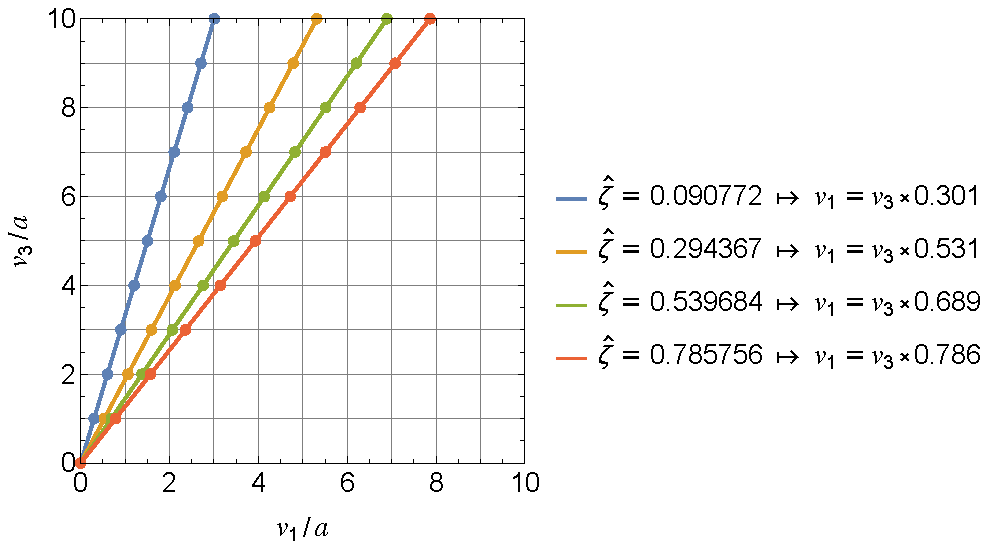
\includegraphics[width=\linewidth]{v1_v2_allzetahat_plot.pdf}
    \end{column}
  \end{columns}
\end{frame}

% Slide 24
\begin{frame}{Bounding lattice paths for each momentum}
  \quick
  \centering
  \begin{tabular}{cc}
    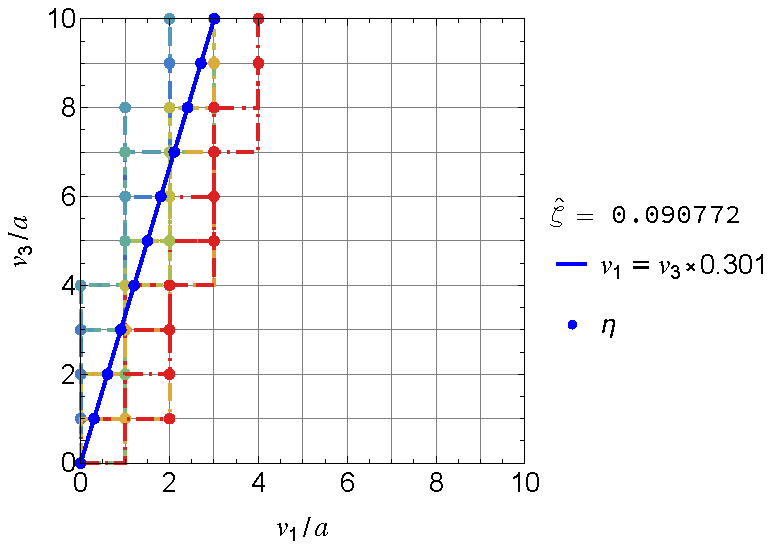
\includegraphics[height=0.37\textheight]{v1_v2_withPath_forP-1_plot.pdf} &
    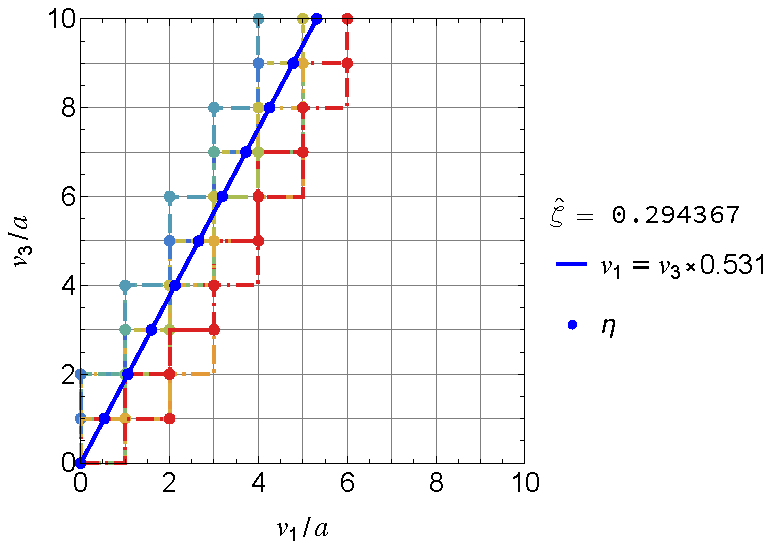
\includegraphics[height=0.37\textheight]{v1_v2_withPath_forP-2_plot.pdf} \\[-1mm]
    {\scriptsize $P_L=-1$, $\zetahat=0.090772$} & {\scriptsize $P_L=-2$, $\zetahat=0.294367$} \\
    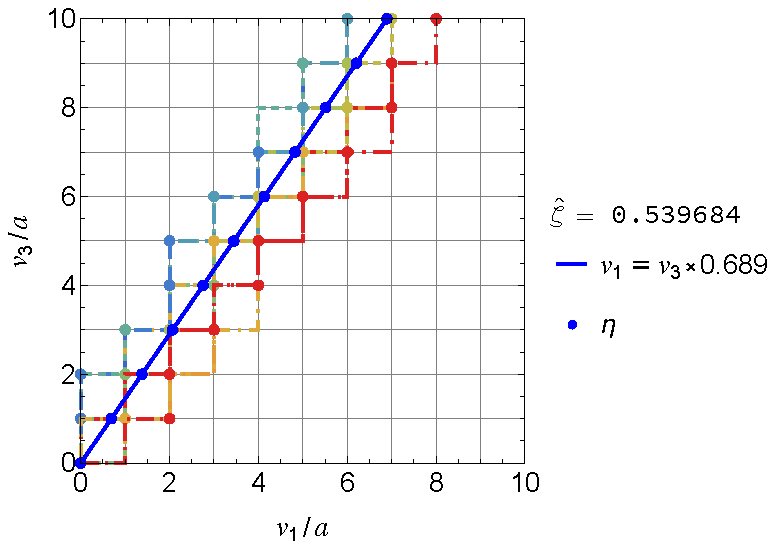
\includegraphics[height=0.37\textheight]{v1_v2_withPath_forP-3_plot.pdf} &
    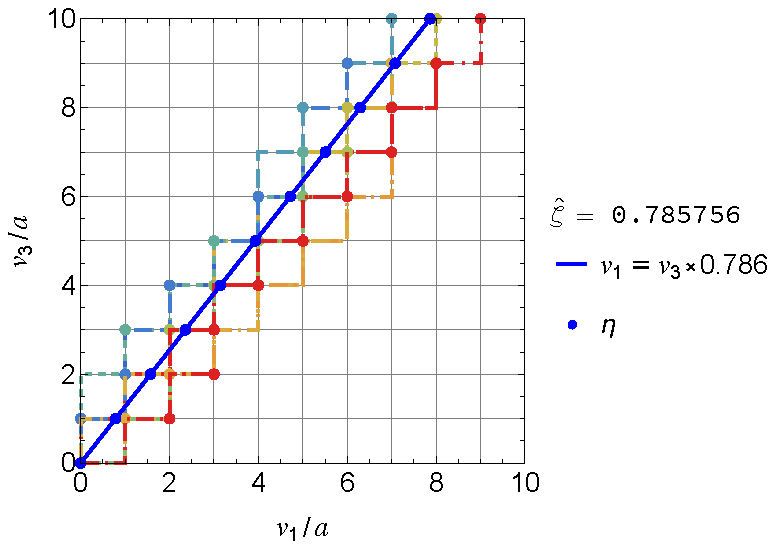
\includegraphics[height=0.37\textheight]{v1_v2_withPath_forP-4_plot.pdf} \\[-1mm]
    {\scriptsize $P_L=-3$, $\zetahat=0.539684$} & {\scriptsize $P_L=-4$, $\zetahat=0.785756$}
  \end{tabular}
\end{frame}

% Slide 25
\begin{frame}{Staple link paths at $P_L=-1$}
  \quick
  \begin{columns}[c]
    \begin{column}{0.36\textwidth}
      \centering
      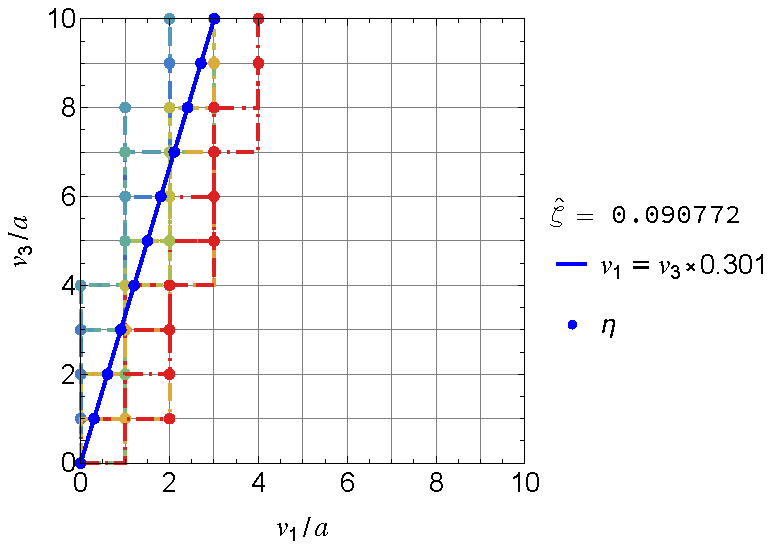
\includegraphics[width=\linewidth]{v1_v2_withPath_forP-1_plot.pdf}\\
      {\scriptsize Integer lattice sites bounding $\eta\vect v/a$}
      \begin{itemize}
        \item For each $\eta$ we compute the correlator at several bounding sites around the target.
      \end{itemize}
    \end{column}
    \begin{column}{0.62\textwidth}
      \centering
      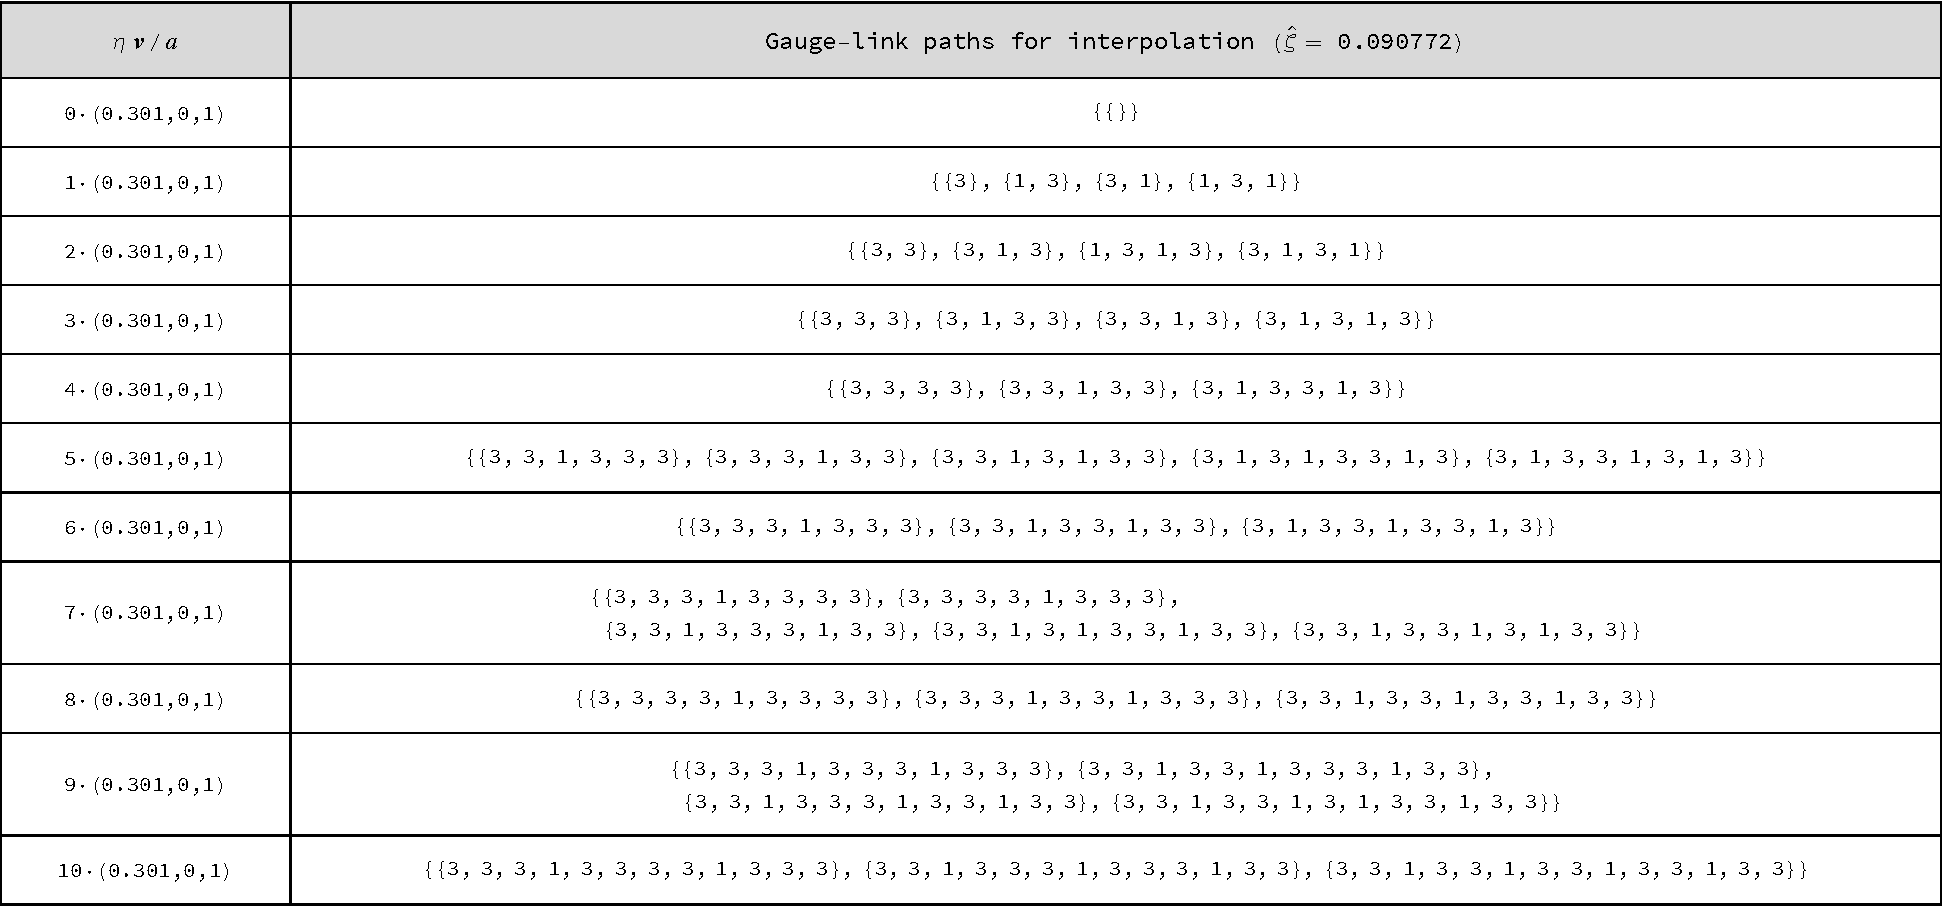
\includegraphics[width=\linewidth]{eta_gauge_links_forP-1_table.pdf}\\
      {\scriptsize Gauge-link step sequences used for interpolation ($\zetahat=0.090772$)}
    \end{column}
  \end{columns}
\end{frame}

\begin{frame}{Staple interpolation paths at $P_L=-2$}
\centering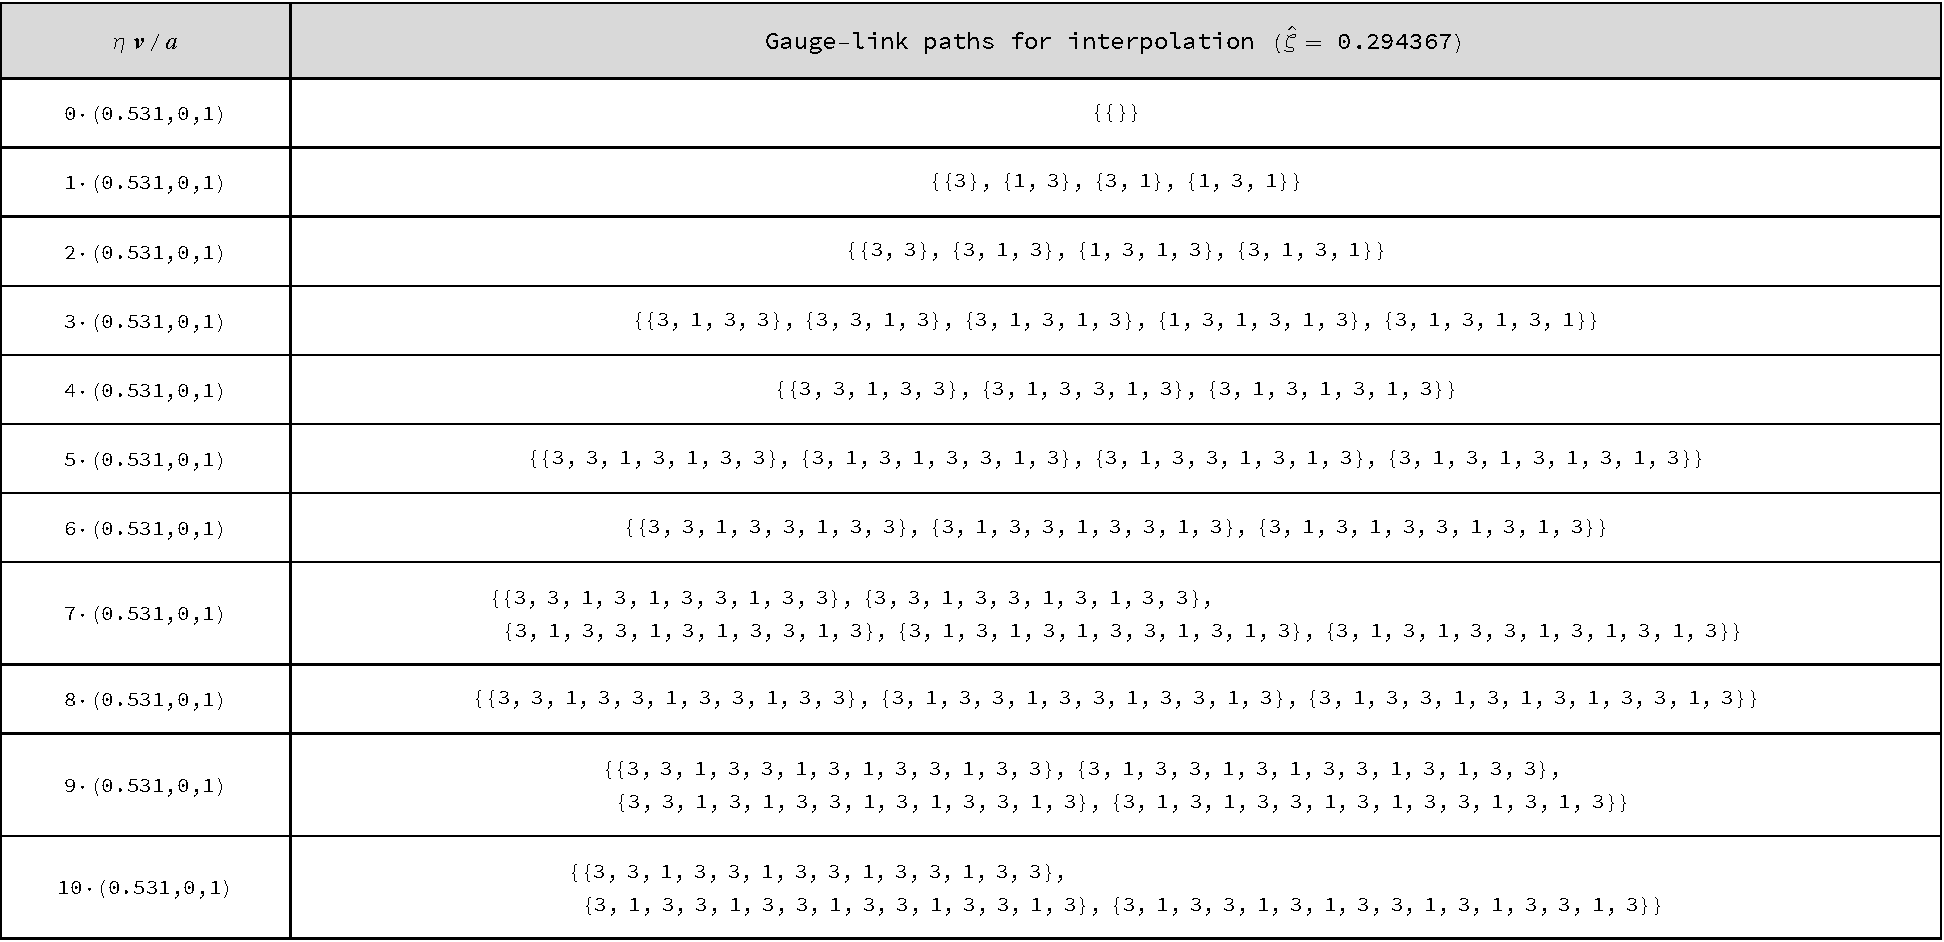
\includegraphics[width=0.97\linewidth,height=0.76\textheight,keepaspectratio]{eta_gauge_links_forP-2_table.pdf}
\figsrc{Thesis, Ch. 5: bounding lattice paths. Arrays list the complete directional step sequence.}
\end{frame}

\begin{frame}{Staple interpolation paths at $P_L=-3$}
\centering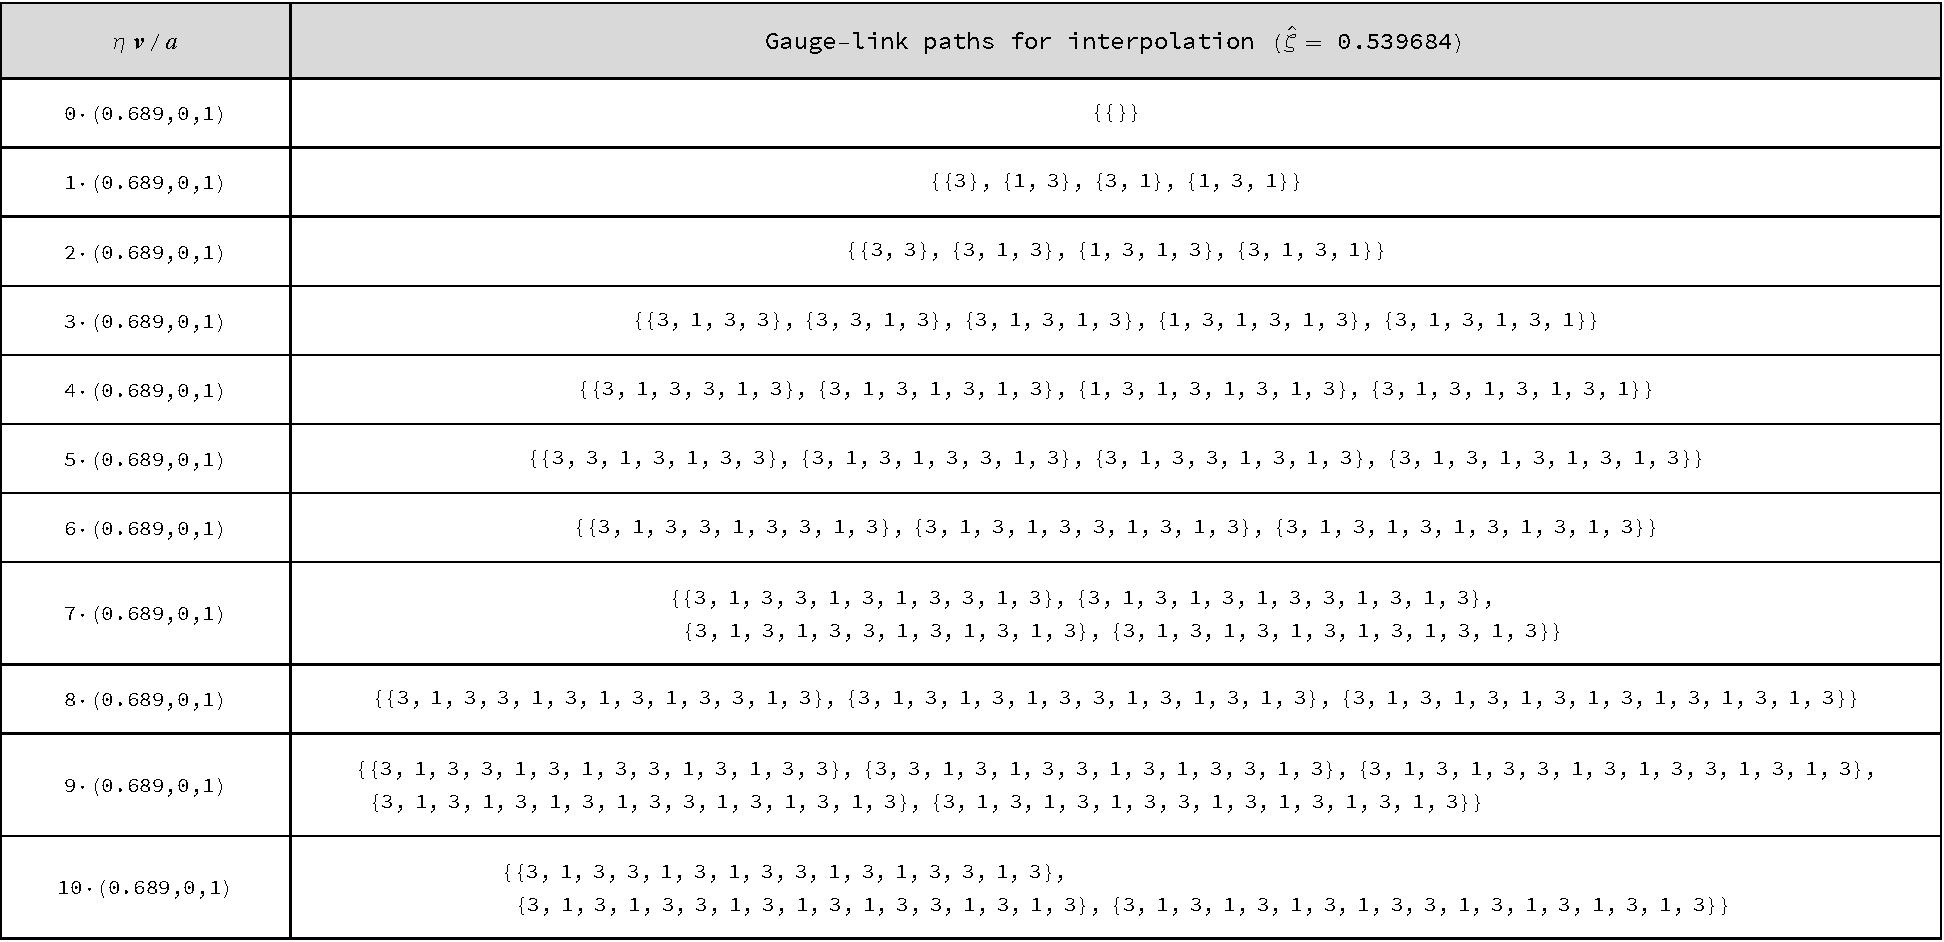
\includegraphics[width=0.97\linewidth,height=0.76\textheight,keepaspectratio]{eta_gauge_links_forP-3_table.pdf}
\figsrc{Thesis, Ch. 5: bounding lattice paths. Arrays list the complete directional step sequence.}
\end{frame}

\begin{frame}{Staple interpolation paths at $P_L=-4$}
\centering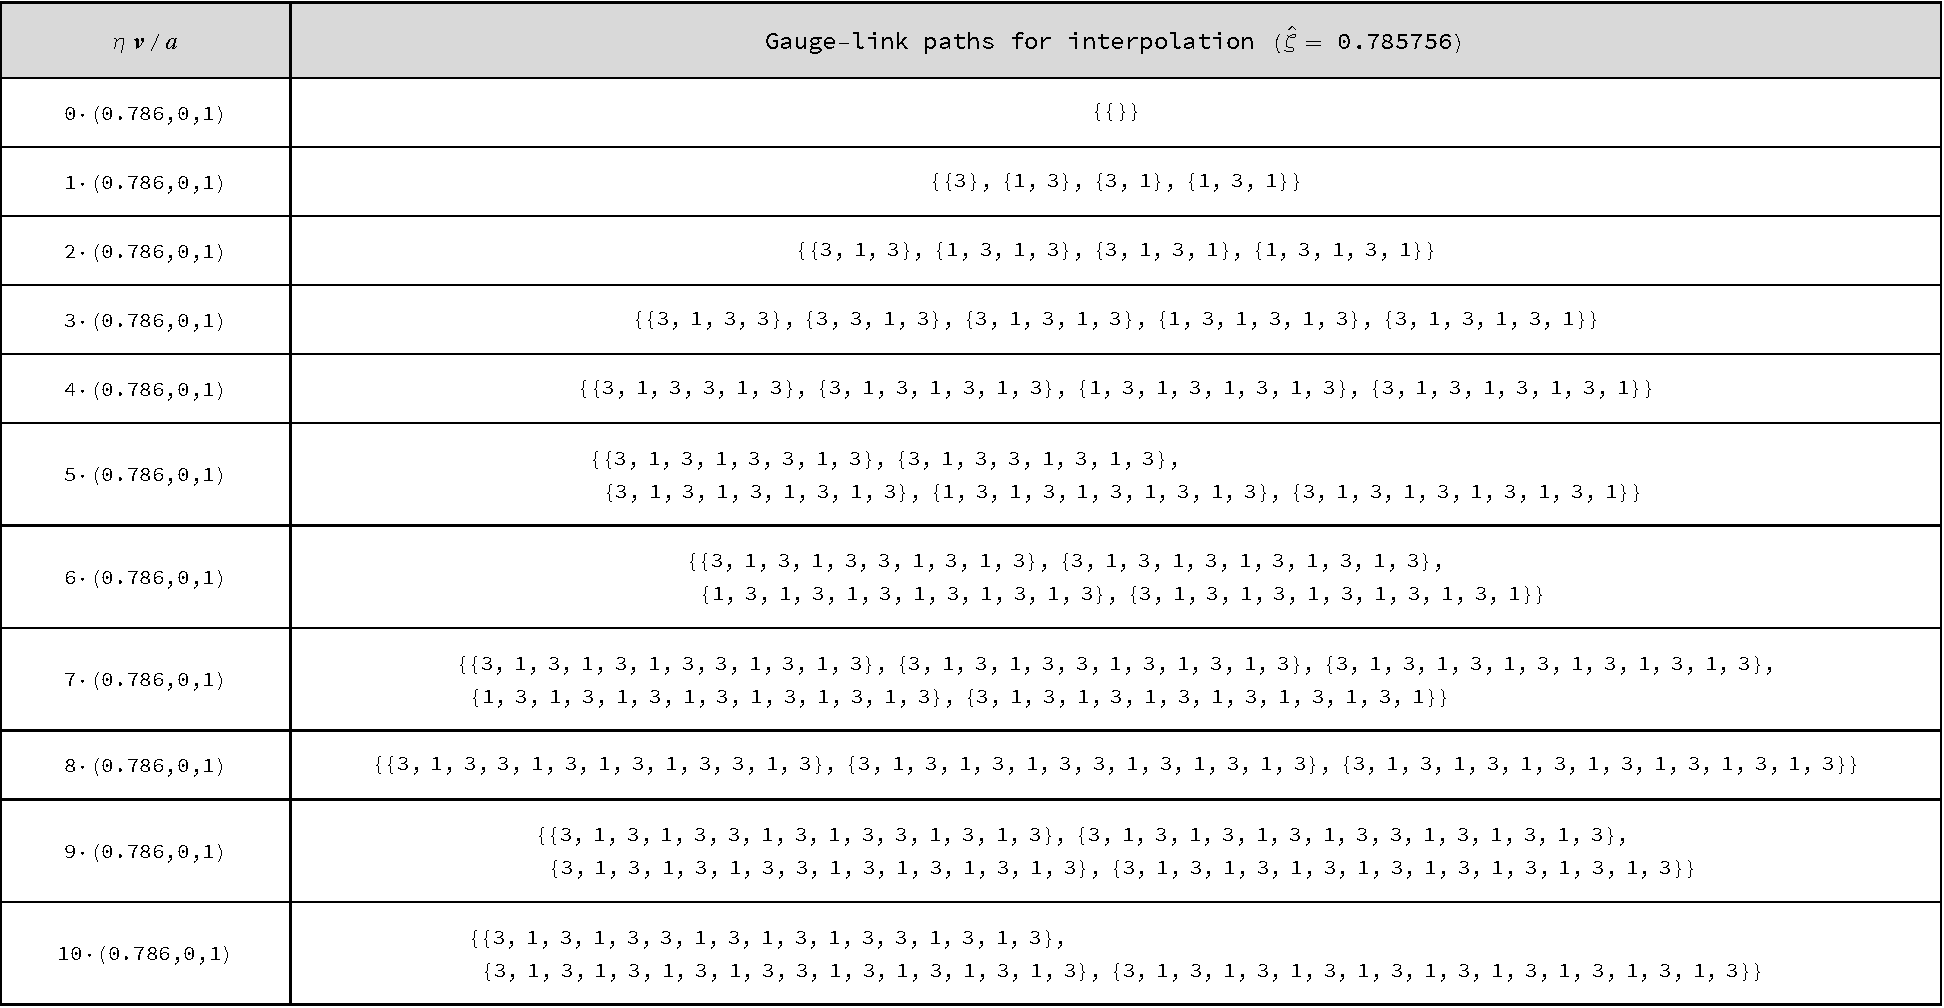
\includegraphics[width=0.97\linewidth,height=0.76\textheight,keepaspectratio]{eta_gauge_links_forP-4_table.pdf}
\figsrc{Thesis, Ch. 5: bounding lattice paths. Arrays list the complete directional step sequence.}
\end{frame}
\begin{frame}{Staple path sequences: $P_L=-1$, $\eta=0$--$2$}
\centering\small
\begin{tabular}{r l}
$\eta=0$ & $\eta\,( 0.301,0,1)$\\
& $\{\}$\\
\noalign{\vskip2pt}
$\eta=1$ & $\eta\,( 0.301,0,1)$\\
& $\{3\}$\\
& $\{1, 3\}$\\
& $\{3, 1\}$\\
& $\{1, 3, 1\}$\\
\noalign{\vskip2pt}
$\eta=2$ & $\eta\,( 0.301,0,1)$\\
& $\{3, 3\}$\\
& $\{3, 1, 3\}$\\
& $\{1, 3, 1, 3\}$\\
& $\{3, 1, 3, 1\}$\\
\noalign{\vskip2pt}
\end{tabular}
\figsrc{Thesis, Ch. 5: full bounding-path sequences. Each row is one ordered lattice path; 1 and 3 denote spatial directions.}
\end{frame}

\begin{frame}{Staple path sequences: $P_L=-1$, $\eta=3$--$4$}
\centering\small
\begin{tabular}{r l}
$\eta=3$ & $\eta\,( 0.301,0,1)$\\
& $\{3, 3, 3\}$\\
& $\{3, 1, 3, 3\}$\\
& $\{3, 3, 1, 3\}$\\
& $\{3, 1, 3, 1, 3\}$\\
\noalign{\vskip2pt}
$\eta=4$ & $\eta\,( 0.301,0,1)$\\
& $\{3, 3, 3, 3\}$\\
& $\{3, 3, 1, 3, 3\}$\\
& $\{3, 1, 3, 3, 1, 3\}$\\
\noalign{\vskip2pt}
\end{tabular}
\figsrc{Thesis, Ch. 5: full bounding-path sequences. Each row is one ordered lattice path; 1 and 3 denote spatial directions.}
\end{frame}

\begin{frame}{Staple path sequences: $P_L=-1$, $\eta=5$--$6$}
\centering\small
\begin{tabular}{r l}
$\eta=5$ & $\eta\,( 0.301,0,1)$\\
& $\{3, 3, 1, 3, 3, 3\}$\\
& $\{3, 3, 3, 1, 3, 3\}$\\
& $\{3, 3, 1, 3, 1, 3, 3\}$\\
& $\{3, 1, 3, 1, 3, 3, 1, 3\}$\\
& $\{3, 1, 3, 3, 1, 3, 1, 3\}$\\
\noalign{\vskip2pt}
$\eta=6$ & $\eta\,( 0.301,0,1)$\\
& $\{3, 3, 3, 1, 3, 3, 3\}$\\
& $\{3, 3, 1, 3, 3, 1, 3, 3\}$\\
& $\{3, 1, 3, 3, 1, 3, 3, 1, 3\}$\\
\noalign{\vskip2pt}
\end{tabular}
\figsrc{Thesis, Ch. 5: full bounding-path sequences. Each row is one ordered lattice path; 1 and 3 denote spatial directions.}
\end{frame}

\begin{frame}{Staple path sequences: $P_L=-1$, $\eta=7$--$8$}
\centering\small
\begin{tabular}{r l}
$\eta=7$ & $\eta\,( 0.301,0,1)$\\
& $\{3, 3, 3, 1, 3, 3, 3, 3\}$\\
& $\{3, 3, 3, 3, 1, 3, 3, 3\}$\\
& $\{3, 3, 1, 3, 3, 3, 1, 3, 3\}$\\
& $\{3, 3, 1, 3, 1, 3, 3, 1, 3, 3\}$\\
& $\{3, 3, 1, 3, 3, 1, 3, 1, 3, 3\}$\\
\noalign{\vskip2pt}
$\eta=8$ & $\eta\,( 0.301,0,1)$\\
& $\{3, 3, 3, 3, 1, 3, 3, 3, 3\}$\\
& $\{3, 3, 3, 1, 3, 3, 1, 3, 3, 3\}$\\
& $\{3, 3, 1, 3, 3, 1, 3, 3, 1, 3, 3\}$\\
\noalign{\vskip2pt}
\end{tabular}
\figsrc{Thesis, Ch. 5: full bounding-path sequences. Each row is one ordered lattice path; 1 and 3 denote spatial directions.}
\end{frame}

\begin{frame}{Staple path sequences: $P_L=-1$, $\eta=9$--$10$}
\centering\small
\begin{tabular}{r l}
$\eta=9$ & $\eta\,( 0.301,0,1)$\\
& $\{3, 3, 3, 1, 3, 3, 3, 1, 3, 3, 3\}$\\
& $\{3, 3, 1, 3, 3, 1, 3, 3, 3, 1, 3, 3\}$\\
& $\{3, 3, 1, 3, 3, 3, 1, 3, 3, 1, 3, 3\}$\\
& $\{3, 3, 1, 3, 3, 1, 3, 1, 3, 3, 1, 3, 3\}$\\
\noalign{\vskip2pt}
$\eta=10$ & $\eta\,( 0.301,0,1)$\\
& $\{3, 3, 3, 1, 3, 3, 3, 3, 1, 3, 3, 3\}$\\
& $\{3, 3, 1, 3, 3, 3, 1, 3, 3, 3, 1, 3, 3\}$\\
& $\{3, 3, 1, 3, 3, 1, 3, 3, 1, 3, 3, 1, 3, 3\}$\\
\noalign{\vskip2pt}
\end{tabular}
\figsrc{Thesis, Ch. 5: full bounding-path sequences. Each row is one ordered lattice path; 1 and 3 denote spatial directions.}
\end{frame}

\begin{frame}{Staple path sequences: $P_L=-2$, $\eta=0$--$2$}
\centering\small
\begin{tabular}{r l}
$\eta=0$ & $\eta\,( 0.531,0,1)$\\
& $\{\}$\\
\noalign{\vskip2pt}
$\eta=1$ & $\eta\,( 0.531,0,1)$\\
& $\{3\}$\\
& $\{1, 3\}$\\
& $\{3, 1\}$\\
& $\{1, 3, 1\}$\\
\noalign{\vskip2pt}
$\eta=2$ & $\eta\,( 0.531,0,1)$\\
& $\{3, 3\}$\\
& $\{3, 1, 3\}$\\
& $\{1, 3, 1, 3\}$\\
& $\{3, 1, 3, 1\}$\\
\noalign{\vskip2pt}
\end{tabular}
\figsrc{Thesis, Ch. 5: full bounding-path sequences. Each row is one ordered lattice path; 1 and 3 denote spatial directions.}
\end{frame}

\begin{frame}{Staple path sequences: $P_L=-2$, $\eta=3$--$4$}
\centering\small
\begin{tabular}{r l}
$\eta=3$ & $\eta\,( 0.531,0,1)$\\
& $\{3, 1, 3, 3\}$\\
& $\{3, 3, 1, 3\}$\\
& $\{3, 1, 3, 1, 3\}$\\
& $\{1, 3, 1, 3, 1, 3\}$\\
& $\{3, 1, 3, 1, 3, 1\}$\\
\noalign{\vskip2pt}
$\eta=4$ & $\eta\,( 0.531,0,1)$\\
& $\{3, 3, 1, 3, 3\}$\\
& $\{3, 1, 3, 3, 1, 3\}$\\
& $\{3, 1, 3, 1, 3, 1, 3\}$\\
\noalign{\vskip2pt}
\end{tabular}
\figsrc{Thesis, Ch. 5: full bounding-path sequences. Each row is one ordered lattice path; 1 and 3 denote spatial directions.}
\end{frame}

\begin{frame}{Staple path sequences: $P_L=-2$, $\eta=5$--$6$}
\centering\small
\begin{tabular}{r l}
$\eta=5$ & $\eta\,( 0.531,0,1)$\\
& $\{3, 3, 1, 3, 1, 3, 3\}$\\
& $\{3, 1, 3, 1, 3, 3, 1, 3\}$\\
& $\{3, 1, 3, 3, 1, 3, 1, 3\}$\\
& $\{3, 1, 3, 1, 3, 1, 3, 1, 3\}$\\
\noalign{\vskip2pt}
$\eta=6$ & $\eta\,( 0.531,0,1)$\\
& $\{3, 3, 1, 3, 3, 1, 3, 3\}$\\
& $\{3, 1, 3, 3, 1, 3, 3, 1, 3\}$\\
& $\{3, 1, 3, 1, 3, 3, 1, 3, 1, 3\}$\\
\noalign{\vskip2pt}
\end{tabular}
\figsrc{Thesis, Ch. 5: full bounding-path sequences. Each row is one ordered lattice path; 1 and 3 denote spatial directions.}
\end{frame}

\begin{frame}{Staple path sequences: $P_L=-2$, $\eta=7$--$8$}
\centering\small
\begin{tabular}{r l}
$\eta=7$ & $\eta\,( 0.531,0,1)$\\
& $\{3, 3, 1, 3, 1, 3, 3, 1, 3, 3\}$\\
& $\{3, 3, 1, 3, 3, 1, 3, 1, 3, 3\}$\\
& $\{3, 1, 3, 3, 1, 3, 1, 3, 3, 1, 3\}$\\
& $\{3, 1, 3, 1, 3, 1, 3, 3, 1, 3, 1, 3\}$\\
& $\{3, 1, 3, 1, 3, 3, 1, 3, 1, 3, 1, 3\}$\\
\noalign{\vskip2pt}
$\eta=8$ & $\eta\,( 0.531,0,1)$\\
& $\{3, 3, 1, 3, 3, 1, 3, 3, 1, 3, 3\}$\\
& $\{3, 1, 3, 3, 1, 3, 3, 1, 3, 3, 1, 3\}$\\
& $\{3, 1, 3, 3, 1, 3, 1, 3, 1, 3, 3, 1, 3\}$\\
\noalign{\vskip2pt}
\end{tabular}
\figsrc{Thesis, Ch. 5: full bounding-path sequences. Each row is one ordered lattice path; 1 and 3 denote spatial directions.}
\end{frame}

\begin{frame}{Staple path sequences: $P_L=-2$, $\eta=9$--$10$}
\centering\small
\begin{tabular}{r l}
$\eta=9$ & $\eta\,( 0.531,0,1)$\\
& $\{3, 3, 1, 3, 3, 1, 3, 1, 3, 3, 1, 3, 3\}$\\
& $\{3, 1, 3, 3, 1, 3, 1, 3, 3, 1, 3, 1, 3, 3\}$\\
& $\{3, 3, 1, 3, 1, 3, 3, 1, 3, 1, 3, 3, 1, 3\}$\\
& $\{3, 1, 3, 1, 3, 3, 1, 3, 1, 3, 3, 1, 3, 1, 3\}$\\
\noalign{\vskip2pt}
$\eta=10$ & $\eta\,( 0.531,0,1)$\\
& $\{3, 3, 1, 3, 3, 1, 3, 3, 1, 3, 3, 1, 3, 3\}$\\
& $\{3, 1, 3, 3, 1, 3, 3, 1, 3, 3, 1, 3, 3, 1, 3\}$\\
& $\{3, 1, 3, 3, 1, 3, 1, 3, 3, 1, 3, 1, 3, 3, 1, 3\}$\\
\noalign{\vskip2pt}
\end{tabular}
\figsrc{Thesis, Ch. 5: full bounding-path sequences. Each row is one ordered lattice path; 1 and 3 denote spatial directions.}
\end{frame}

\begin{frame}{Staple path sequences: $P_L=-3$, $\eta=0$--$2$}
\centering\small
\begin{tabular}{r l}
$\eta=0$ & $\eta\,( 0.689,0,1)$\\
& $\{\}$\\
\noalign{\vskip2pt}
$\eta=1$ & $\eta\,( 0.689,0,1)$\\
& $\{3\}$\\
& $\{1, 3\}$\\
& $\{3, 1\}$\\
& $\{1, 3, 1\}$\\
\noalign{\vskip2pt}
$\eta=2$ & $\eta\,( 0.689,0,1)$\\
& $\{3, 3\}$\\
& $\{3, 1, 3\}$\\
& $\{1, 3, 1, 3\}$\\
& $\{3, 1, 3, 1\}$\\
\noalign{\vskip2pt}
\end{tabular}
\figsrc{Thesis, Ch. 5: full bounding-path sequences. Each row is one ordered lattice path; 1 and 3 denote spatial directions.}
\end{frame}

\begin{frame}{Staple path sequences: $P_L=-3$, $\eta=3$--$4$}
\centering\small
\begin{tabular}{r l}
$\eta=3$ & $\eta\,( 0.689,0,1)$\\
& $\{3, 1, 3, 3\}$\\
& $\{3, 3, 1, 3\}$\\
& $\{3, 1, 3, 1, 3\}$\\
& $\{1, 3, 1, 3, 1, 3\}$\\
& $\{3, 1, 3, 1, 3, 1\}$\\
\noalign{\vskip2pt}
$\eta=4$ & $\eta\,( 0.689,0,1)$\\
& $\{3, 1, 3, 3, 1, 3\}$\\
& $\{3, 1, 3, 1, 3, 1, 3\}$\\
& $\{1, 3, 1, 3, 1, 3, 1, 3\}$\\
& $\{3, 1, 3, 1, 3, 1, 3, 1\}$\\
\noalign{\vskip2pt}
\end{tabular}
\figsrc{Thesis, Ch. 5: full bounding-path sequences. Each row is one ordered lattice path; 1 and 3 denote spatial directions.}
\end{frame}

\begin{frame}{Staple path sequences: $P_L=-3$, $\eta=5$--$6$}
\centering\small
\begin{tabular}{r l}
$\eta=5$ & $\eta\,( 0.689,0,1)$\\
& $\{3, 3, 1, 3, 1, 3, 3\}$\\
& $\{3, 1, 3, 1, 3, 3, 1, 3\}$\\
& $\{3, 1, 3, 3, 1, 3, 1, 3\}$\\
& $\{3, 1, 3, 1, 3, 1, 3, 1, 3\}$\\
\noalign{\vskip2pt}
$\eta=6$ & $\eta\,( 0.689,0,1)$\\
& $\{3, 1, 3, 3, 1, 3, 3, 1, 3\}$\\
& $\{3, 1, 3, 1, 3, 3, 1, 3, 1, 3\}$\\
& $\{3, 1, 3, 1, 3, 1, 3, 1, 3, 1, 3\}$\\
\noalign{\vskip2pt}
\end{tabular}
\figsrc{Thesis, Ch. 5: full bounding-path sequences. Each row is one ordered lattice path; 1 and 3 denote spatial directions.}
\end{frame}

\begin{frame}{Staple path sequences: $P_L=-3$, $\eta=7$--$8$}
\centering\small
\begin{tabular}{r l}
$\eta=7$ & $\eta\,( 0.689,0,1)$\\
& $\{3, 1, 3, 3, 1, 3, 1, 3, 3, 1, 3\}$\\
& $\{3, 1, 3, 1, 3, 1, 3, 3, 1, 3, 1, 3\}$\\
& $\{3, 1, 3, 1, 3, 3, 1, 3, 1, 3, 1, 3\}$\\
& $\{3, 1, 3, 1, 3, 1, 3, 1, 3, 1, 3, 1, 3\}$\\
\noalign{\vskip2pt}
$\eta=8$ & $\eta\,( 0.689,0,1)$\\
& $\{3, 1, 3, 3, 1, 3, 1, 3, 1, 3, 3, 1, 3\}$\\
& $\{3, 1, 3, 1, 3, 1, 3, 3, 1, 3, 1, 3, 1, 3\}$\\
& $\{3, 1, 3, 1, 3, 1, 3, 1, 3, 1, 3, 1, 3, 1, 3\}$\\
\noalign{\vskip2pt}
\end{tabular}
\figsrc{Thesis, Ch. 5: full bounding-path sequences. Each row is one ordered lattice path; 1 and 3 denote spatial directions.}
\end{frame}

\begin{frame}{Staple path sequences: $P_L=-3$, $\eta=9$--$10$}
\centering\small
\begin{tabular}{r l}
$\eta=9$ & $\eta\,( 0.689,0,1)$\\
& $\{3, 1, 3, 3, 1, 3, 1, 3, 3, 1, 3, 1, 3, 3\}$\\
& $\{3, 3, 1, 3, 1, 3, 3, 1, 3, 1, 3, 3, 1, 3\}$\\
& $\{3, 1, 3, 1, 3, 3, 1, 3, 1, 3, 3, 1, 3, 1, 3\}$\\
& $\{3, 1, 3, 1, 3, 1, 3, 1, 3, 3, 1, 3, 1, 3, 1, 3\}$\\
& $\{3, 1, 3, 1, 3, 1, 3, 3, 1, 3, 1, 3, 1, 3, 1, 3\}$\\
\noalign{\vskip2pt}
$\eta=10$ & $\eta\,( 0.689,0,1)$\\
& $\{3, 1, 3, 3, 1, 3, 1, 3, 3, 1, 3, 1, 3, 3, 1, 3\}$\\
& $\{3, 1, 3, 1, 3, 3, 1, 3, 1, 3, 1, 3, 3, 1, 3, 1, 3\}$\\
& $\{3, 1, 3, 1, 3, 1, 3, 1, 3, 3, 1, 3, 1, 3, 1, 3, 1, 3\}$\\
\noalign{\vskip2pt}
\end{tabular}
\figsrc{Thesis, Ch. 5: full bounding-path sequences. Each row is one ordered lattice path; 1 and 3 denote spatial directions.}
\end{frame}

\begin{frame}{Staple path sequences: $P_L=-4$, $\eta=0$--$2$}
\centering\small
\begin{tabular}{r l}
$\eta=0$ & $\eta\,( 0.786,0,1)$\\
& $\{\}$\\
\noalign{\vskip2pt}
$\eta=1$ & $\eta\,( 0.786,0,1)$\\
& $\{3\}$\\
& $\{1, 3\}$\\
& $\{3, 1\}$\\
& $\{1, 3, 1\}$\\
\noalign{\vskip2pt}
$\eta=2$ & $\eta\,( 0.786,0,1)$\\
& $\{3, 1, 3\}$\\
& $\{1, 3, 1, 3\}$\\
& $\{3, 1, 3, 1\}$\\
& $\{1, 3, 1, 3, 1\}$\\
\noalign{\vskip2pt}
\end{tabular}
\figsrc{Thesis, Ch. 5: full bounding-path sequences. Each row is one ordered lattice path; 1 and 3 denote spatial directions.}
\end{frame}

\begin{frame}{Staple path sequences: $P_L=-4$, $\eta=3$--$4$}
\centering\small
\begin{tabular}{r l}
$\eta=3$ & $\eta\,( 0.786,0,1)$\\
& $\{3, 1, 3, 3\}$\\
& $\{3, 3, 1, 3\}$\\
& $\{3, 1, 3, 1, 3\}$\\
& $\{1, 3, 1, 3, 1, 3\}$\\
& $\{3, 1, 3, 1, 3, 1\}$\\
\noalign{\vskip2pt}
$\eta=4$ & $\eta\,( 0.786,0,1)$\\
& $\{3, 1, 3, 3, 1, 3\}$\\
& $\{3, 1, 3, 1, 3, 1, 3\}$\\
& $\{1, 3, 1, 3, 1, 3, 1, 3\}$\\
& $\{3, 1, 3, 1, 3, 1, 3, 1\}$\\
\noalign{\vskip2pt}
\end{tabular}
\figsrc{Thesis, Ch. 5: full bounding-path sequences. Each row is one ordered lattice path; 1 and 3 denote spatial directions.}
\end{frame}

\begin{frame}{Staple path sequences: $P_L=-4$, $\eta=5$--$6$}
\centering\small
\begin{tabular}{r l}
$\eta=5$ & $\eta\,( 0.786,0,1)$\\
& $\{3, 1, 3, 1, 3, 3, 1, 3\}$\\
& $\{3, 1, 3, 3, 1, 3, 1, 3\}$\\
& $\{3, 1, 3, 1, 3, 1, 3, 1, 3\}$\\
& $\{1, 3, 1, 3, 1, 3, 1, 3, 1, 3\}$\\
& $\{3, 1, 3, 1, 3, 1, 3, 1, 3, 1\}$\\
\noalign{\vskip2pt}
$\eta=6$ & $\eta\,( 0.786,0,1)$\\
& $\{3, 1, 3, 1, 3, 3, 1, 3, 1, 3\}$\\
& $\{3, 1, 3, 1, 3, 1, 3, 1, 3, 1, 3\}$\\
& $\{1, 3, 1, 3, 1, 3, 1, 3, 1, 3, 1, 3\}$\\
& $\{3, 1, 3, 1, 3, 1, 3, 1, 3, 1, 3, 1\}$\\
\noalign{\vskip2pt}
\end{tabular}
\figsrc{Thesis, Ch. 5: full bounding-path sequences. Each row is one ordered lattice path; 1 and 3 denote spatial directions.}
\end{frame}

\begin{frame}{Staple path sequences: $P_L=-4$, $\eta=7$--$8$}
\centering\small
\begin{tabular}{r l}
$\eta=7$ & $\eta\,( 0.786,0,1)$\\
& $\{3, 1, 3, 1, 3, 1, 3, 3, 1, 3, 1, 3\}$\\
& $\{3, 1, 3, 1, 3, 3, 1, 3, 1, 3, 1, 3\}$\\
& $\{3, 1, 3, 1, 3, 1, 3, 1, 3, 1, 3, 1, 3\}$\\
& $\{1, 3, 1, 3, 1, 3, 1, 3, 1, 3, 1, 3, 1, 3\}$\\
& $\{3, 1, 3, 1, 3, 1, 3, 1, 3, 1, 3, 1, 3, 1\}$\\
\noalign{\vskip2pt}
$\eta=8$ & $\eta\,( 0.786,0,1)$\\
& $\{3, 1, 3, 3, 1, 3, 1, 3, 1, 3, 3, 1, 3\}$\\
& $\{3, 1, 3, 1, 3, 1, 3, 3, 1, 3, 1, 3, 1, 3\}$\\
& $\{3, 1, 3, 1, 3, 1, 3, 1, 3, 1, 3, 1, 3, 1, 3\}$\\
\noalign{\vskip2pt}
\end{tabular}
\figsrc{Thesis, Ch. 5: full bounding-path sequences. Each row is one ordered lattice path; 1 and 3 denote spatial directions.}
\end{frame}

\begin{frame}{Staple path sequences: $P_L=-4$, $\eta=9$--$10$}
\centering\small
\begin{tabular}{r l}
$\eta=9$ & $\eta\,( 0.786,0,1)$\\
& $\{3, 1, 3, 1, 3, 3, 1, 3, 1, 3, 3, 1, 3, 1, 3\}$\\
& $\{3, 1, 3, 1, 3, 1, 3, 1, 3, 3, 1, 3, 1, 3, 1, 3\}$\\
& $\{3, 1, 3, 1, 3, 1, 3, 3, 1, 3, 1, 3, 1, 3, 1, 3\}$\\
& $\{3, 1, 3, 1, 3, 1, 3, 1, 3, 1, 3, 1, 3, 1, 3, 1, 3\}$\\
\noalign{\vskip2pt}
$\eta=10$ & $\eta\,( 0.786,0,1)$\\
& $\{3, 1, 3, 1, 3, 3, 1, 3, 1, 3, 1, 3, 3, 1, 3, 1, 3\}$\\
& $\{3, 1, 3, 1, 3, 1, 3, 1, 3, 3, 1, 3, 1, 3, 1, 3, 1, 3\}$\\
& $\{3, 1, 3, 1, 3, 1, 3, 1, 3, 1, 3, 1, 3, 1, 3, 1, 3, 1, 3\}$\\
\noalign{\vskip2pt}
\end{tabular}
\figsrc{Thesis, Ch. 5: full bounding-path sequences. Each row is one ordered lattice path; 1 and 3 denote spatial directions.}
\end{frame}


% Slide 26
\begin{frame}{Symmetry improvement: path averaging for $v$}
  \begin{columns}[c]
    \begin{column}{0.5\textwidth}
      \begin{itemize}
        \item Lattice links lie along the axes: several step-wise permutations end at the \textbf{same} lattice site.
        \item They are equivalent at the endpoints but carry different discretization artifacts and gauge noise.
        \item \textbf{Symmetry improvement:} average the correlators over all degenerate paths to the same site, before interpolating.
      \end{itemize}
    \end{column}
    \begin{column}{0.48\textwidth}
      \centering
      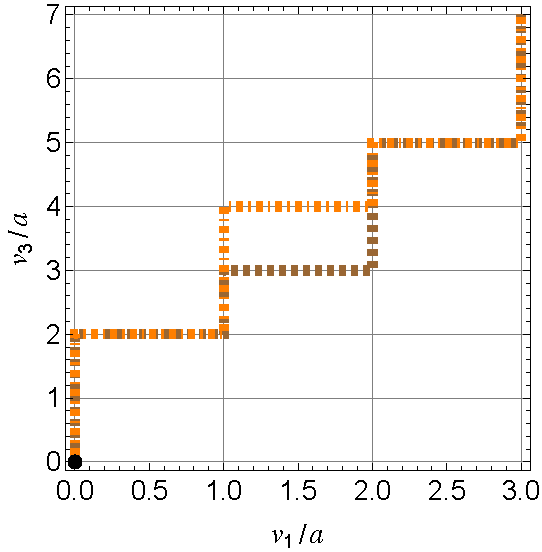
\includegraphics[width=0.85\linewidth]{Example_v_plot_with_2path.pdf}\\
      {\scriptsize Two degenerate paths (solid, dashed) to the same site are averaged.}
    \end{column}
  \end{columns}
\end{frame}

% Slide 27
\begin{frame}{Interpolation to the off-axis direction}
  \begin{columns}[c]
    \begin{column}{0.30\textwidth}
      \[ \Delta v_1 = \frac{v_1^{\text{constraint}} - v_1^{\text{lattice}}}{a} \]
      \begin{itemize}
        \item Path-averaged correlators at three or more bounding sites (red).
        \item Quadratic interpolation in $\Delta v_1$ inside each Jackknife (leave-one-out resampling) sample (grey band).
        \item Read off the value at $\Delta v_1 = 0$ (blue).
        \item All 8 inputs: Re and Im of $R_{\Gamma}$ for $\Gamma=\gamma_1,\gamma_2,\gamma_3,\gamma_4$.
      \end{itemize}
      {\scriptsize $\vect{b}=(1,2,0)$, $\eta=7$, $P_L=-1$}
    \end{column}
    \begin{column}{0.70\textwidth}
      \centering
      \begin{tabular}{@{}c@{\hspace{1mm}}c@{}}
        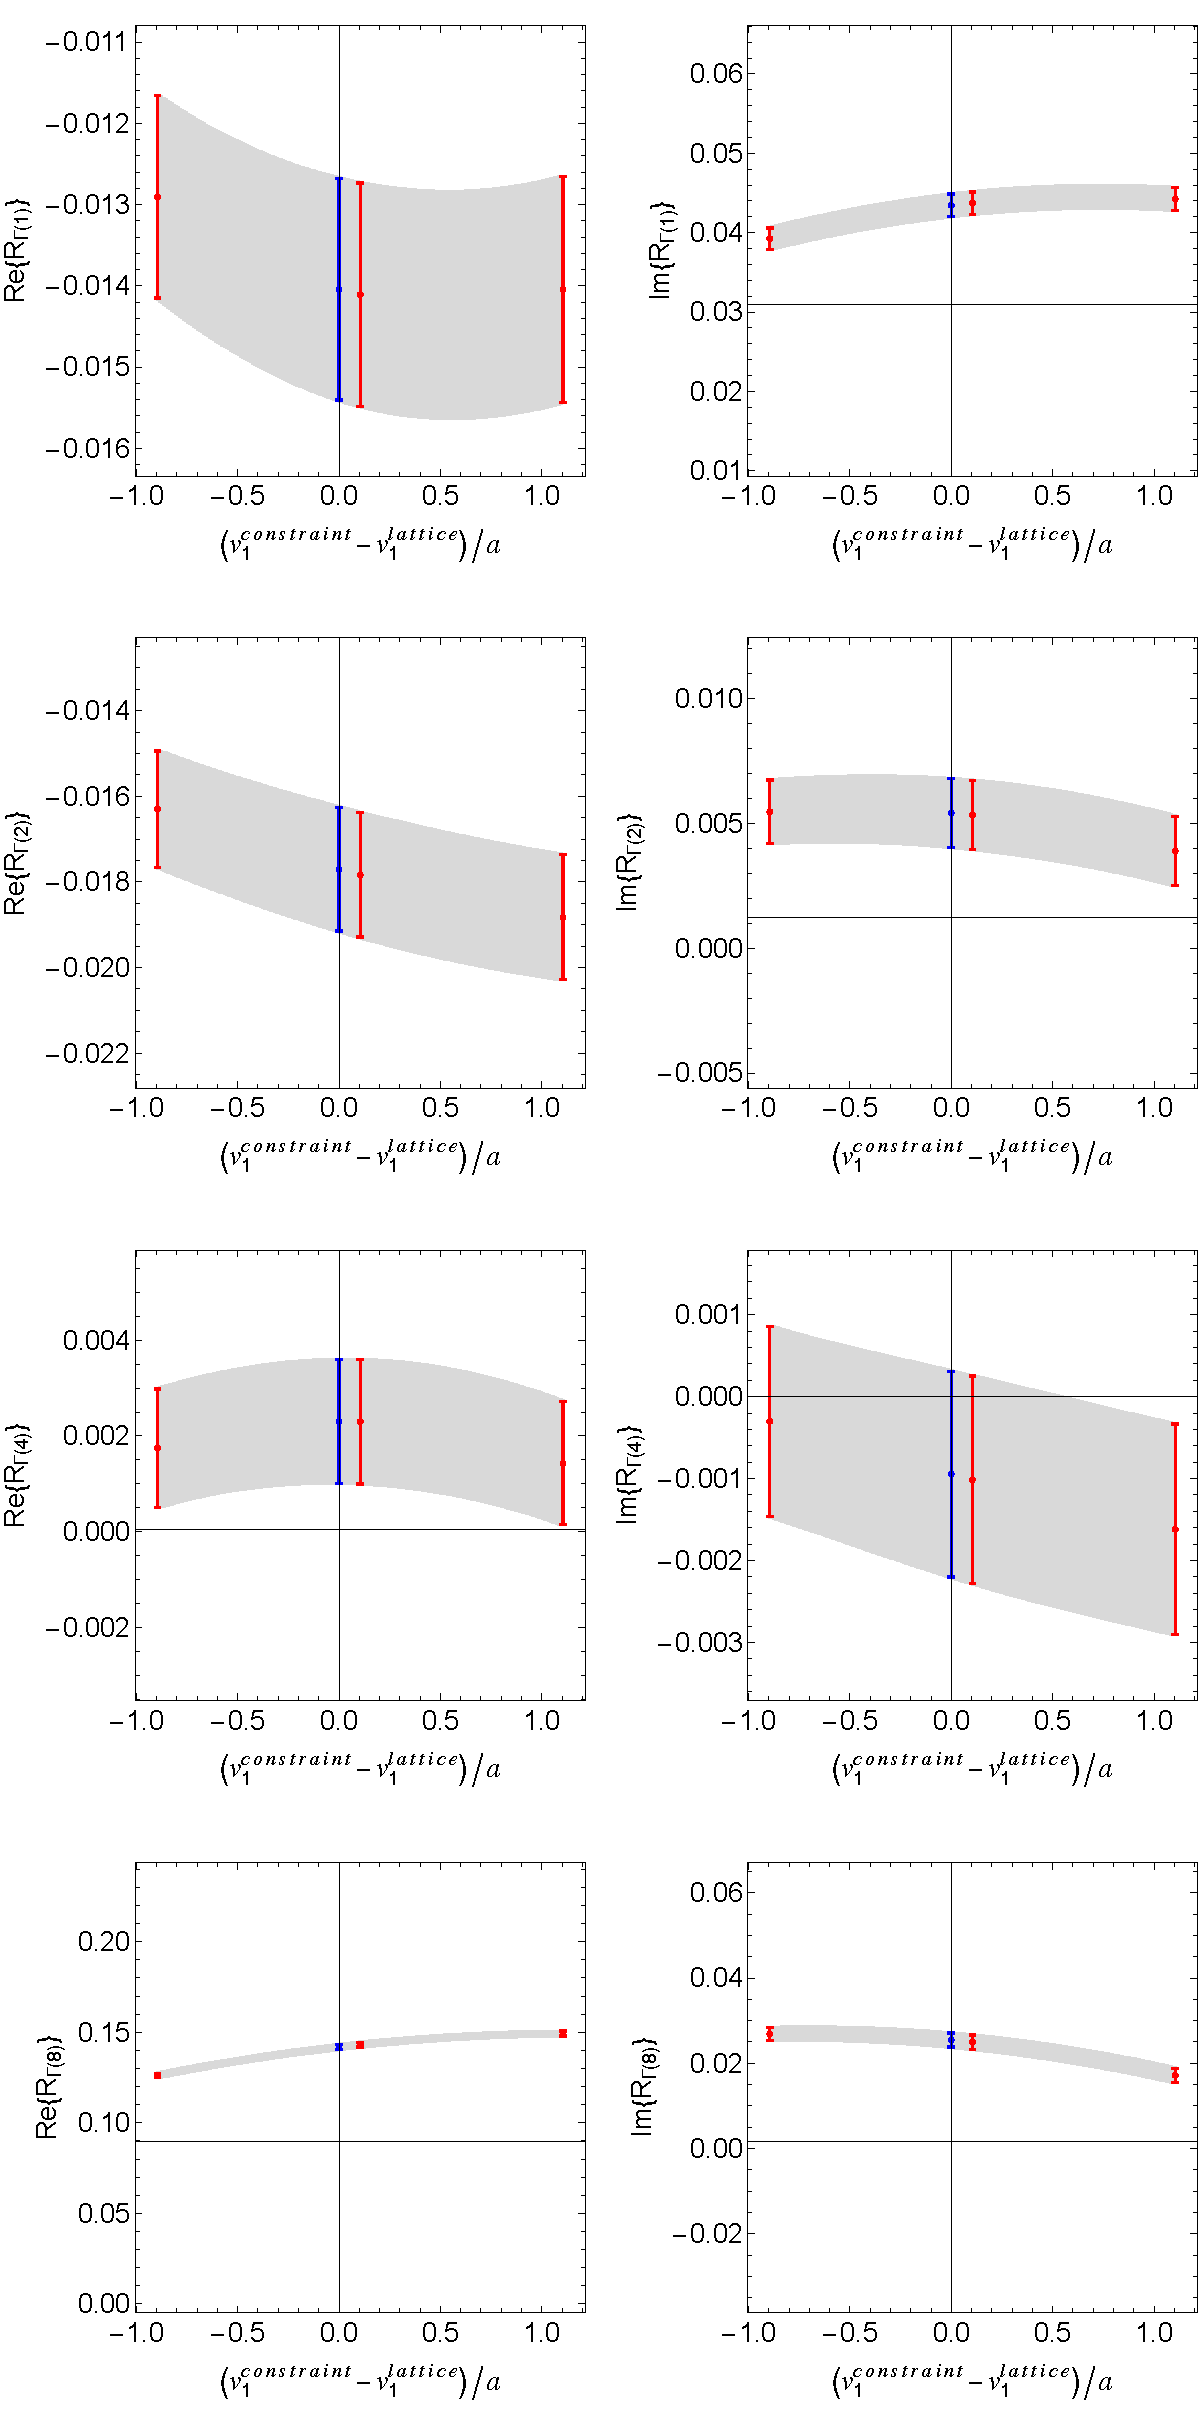
\includegraphics[height=0.6\textheight, trim=0 582 0 0, clip]{Interpolation_Ex_b120_eta7_P-1.pdf} &
        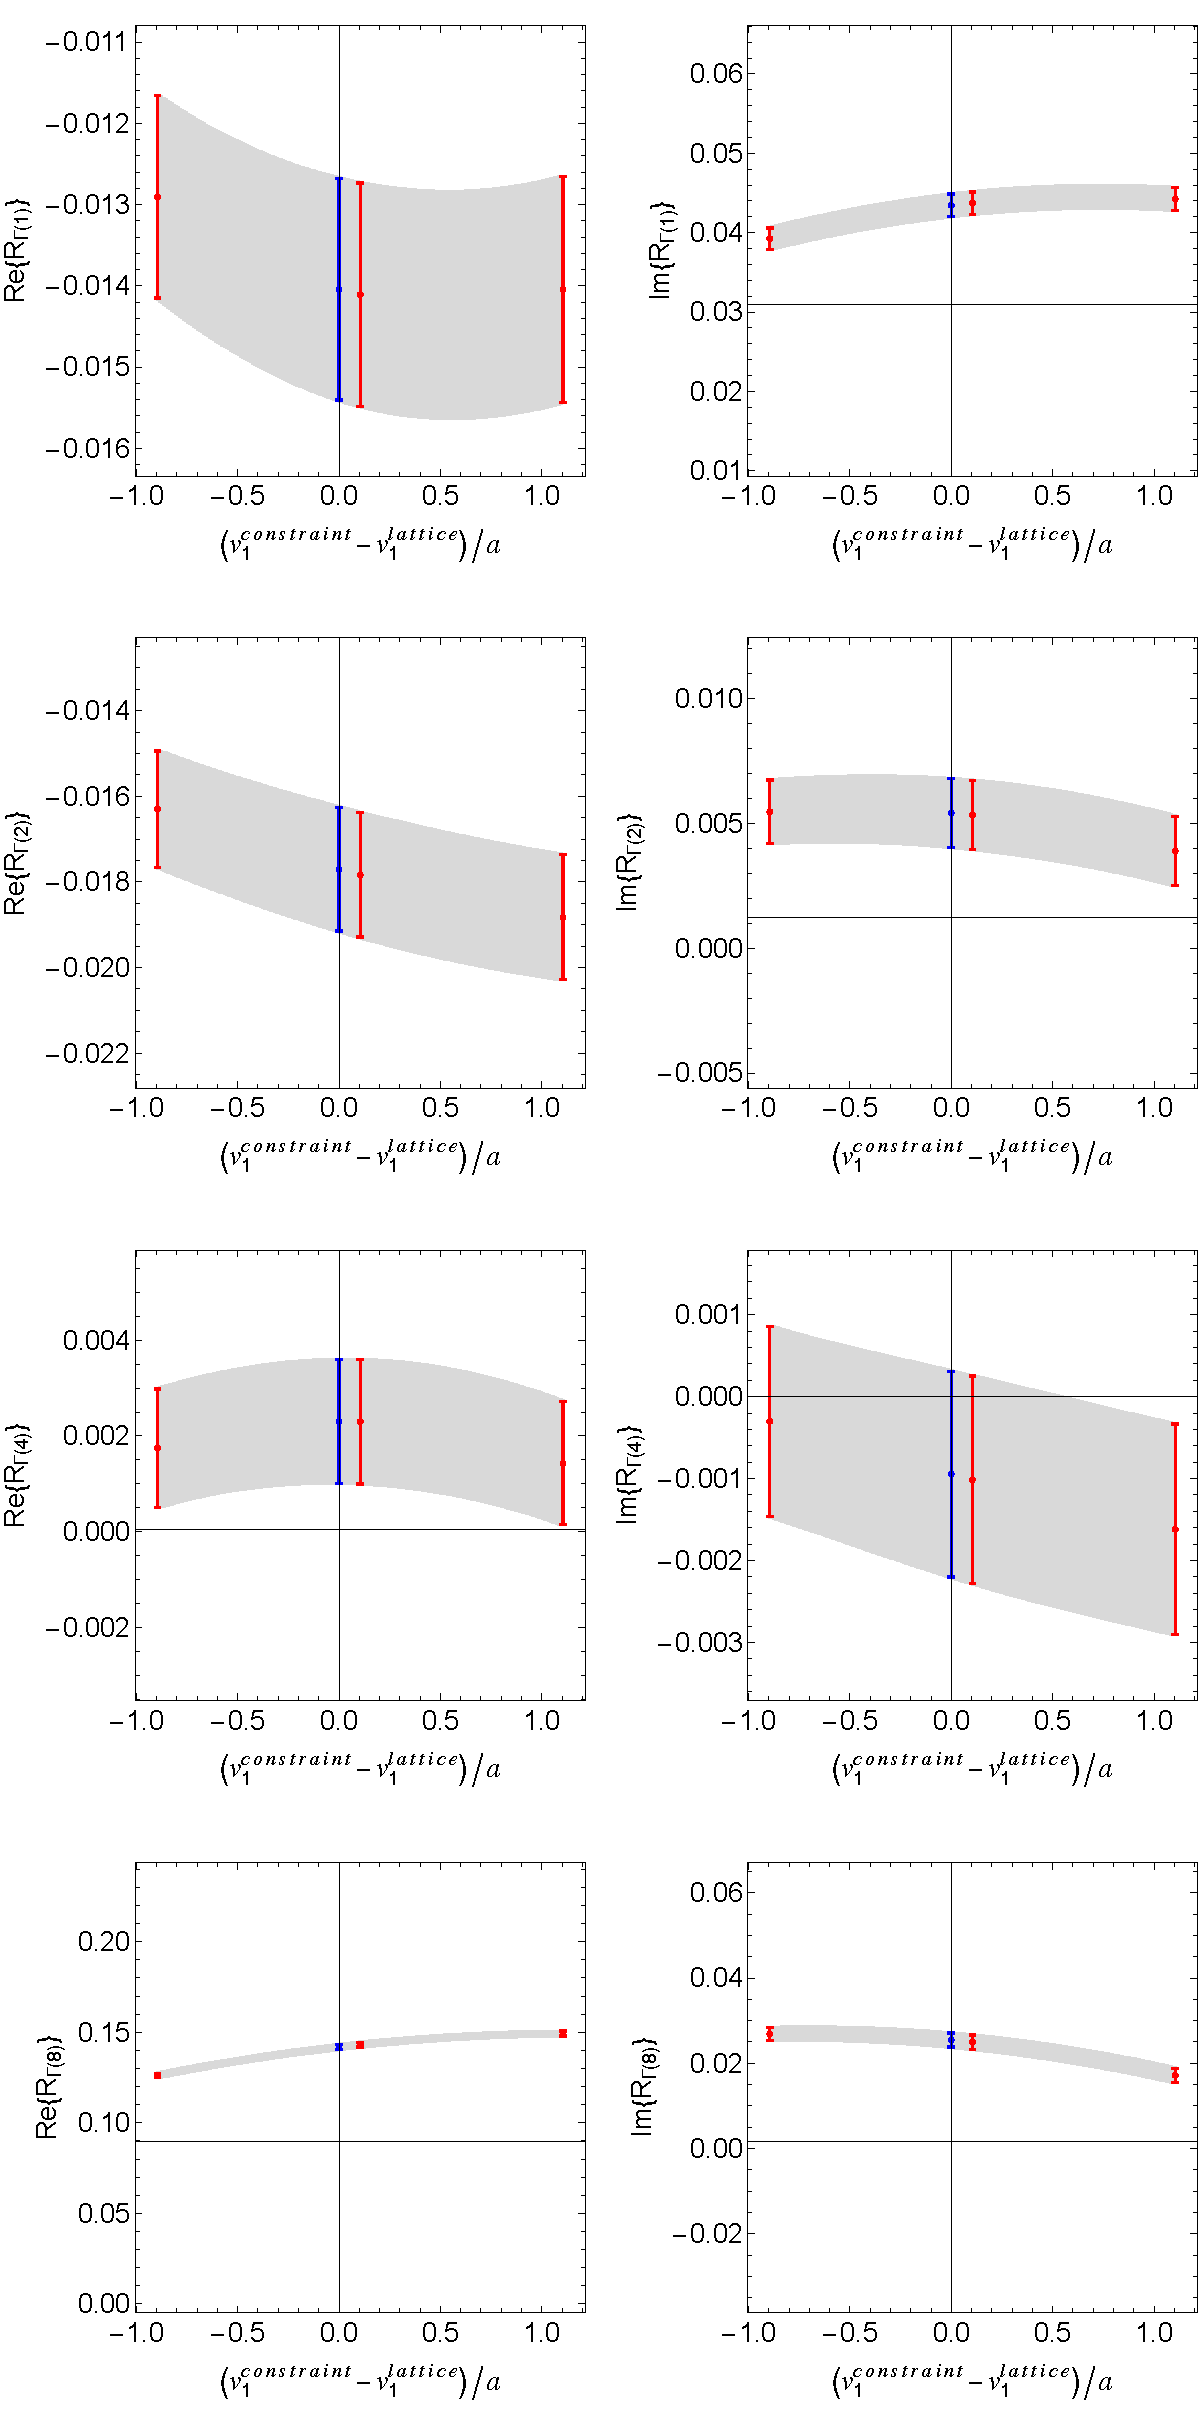
\includegraphics[height=0.6\textheight, trim=0 0 0 582, clip]{Interpolation_Ex_b120_eta7_P-1.pdf} \\
        {\scriptsize $\Gamma=\gamma_1,\gamma_2$: Re (left), Im (right)} & {\scriptsize $\Gamma=\gamma_3,\gamma_4$: Re (left), Im (right)}
      \end{tabular}
    \end{column}
  \end{columns}
\end{frame}

% Slide 28
\begin{frame}{Quark separation vectors $\vect b$}
  \begin{columns}[c]
    \begin{column}{0.4\textwidth}
      \centering
      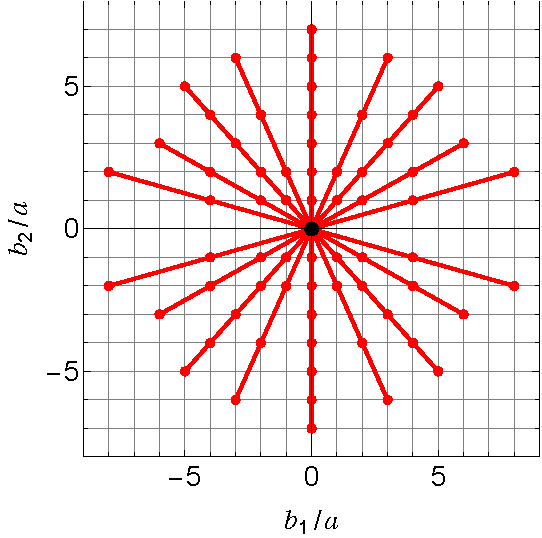
\includegraphics[width=0.9\linewidth]{bL_bT_plot.pdf}\\
      {\scriptsize Sampled $\vect b$ in the $b_1$--$b_2$ plane ($b_1\equiv b_L$, $b_2\equiv b_T$)}
    \end{column}
    \begin{column}{0.58\textwidth}
      \centering
      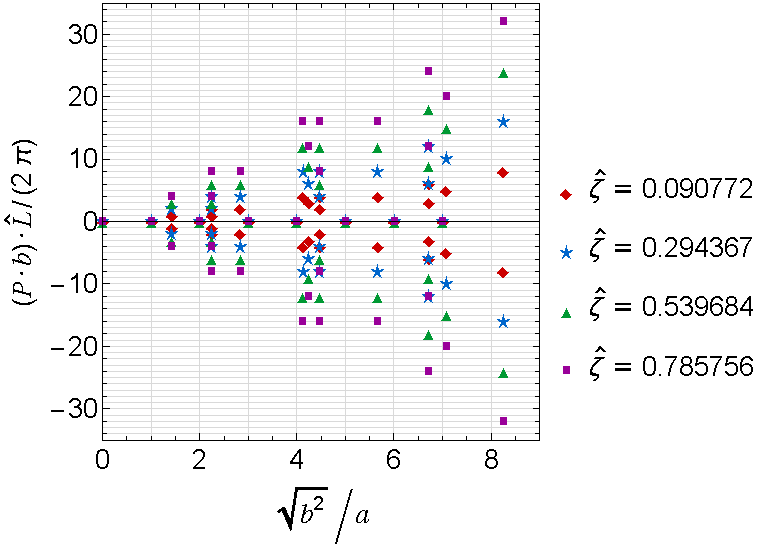
\includegraphics[width=0.95\linewidth]{Pb_bsq_plot.pdf}\\
      {\scriptsize The same vectors in $(\bvec\tcdot P,\ |\vect b|)$ for the four $\zetahat$}
    \end{column}
  \end{columns}
  \begin{itemize}
    \item $P$ along $\hat x_1$: \ $\bvec\cdot P=-P_1 b_1$. Each $+b_1$ has a mirrored $-b_1$, so we reach $\pm\bvec\tcdot P$.
    \item Higher $|P_L|$ stretches the reach in $\bvec\tcdot P$.
  \end{itemize}
\end{frame}

\begin{frame}{Quark-separation path pairs: table 1, part 1}
\label{coverage:bpaths-1-1}
\centering\small
\begin{tabular}{l@{\hspace{12mm}}l}
Coordinate $(b_1,b_2,b_3)/a$ & Reflected coordinate $(-b_1,b_2,b_3)/a$\\\hline
$\{0,0,0\}$ & $\{0,0,0\}$\\
$\{\}$ & $\{\}$\\
\noalign{\vskip3pt}
$\{0,1,0\}$ & $\{0,1,0\}$\\
$\{2\}$ & $\{2\}$\\
\noalign{\vskip3pt}
$\{0,2,0\}$ & $\{0,2,0\}$\\
$\{2,2\}$ & $\{2,2\}$\\
\noalign{\vskip3pt}
$\{0,3,0\}$ & $\{0,3,0\}$\\
$\{2,2,2\}$ & $\{2,2,2\}$\\
\noalign{\vskip3pt}
\end{tabular}
\figsrc{Thesis, Ch. 5: original path entries; a signed integer denotes a directed lattice step.}
\end{frame}

\begin{frame}{Quark-separation path pairs: table 1, part 2}
\label{coverage:bpaths-1-2}
\centering\small
\begin{tabular}{l@{\hspace{12mm}}l}
Coordinate $(b_1,b_2,b_3)/a$ & Reflected coordinate $(-b_1,b_2,b_3)/a$\\\hline
$\{0,4,0\}$ & $\{0,4,0\}$\\
$\{2,2,2,2\}$ & $\{2,2,2,2\}$\\
\noalign{\vskip3pt}
$\{0,5,0\}$ & $\{0,5,0\}$\\
$\{2,2,2,2,2\}$ & $\{2,2,2,2,2\}$\\
\noalign{\vskip3pt}
$\{0,6,0\}$ & $\{0,6,0\}$\\
$\{2,2,2,2,2,2\}$ & $\{2,2,2,2,2,2\}$\\
\noalign{\vskip3pt}
$\{0,7,0\}$ & $\{0,7,0\}$\\
$\{2,2,2,2,2,2,2\}$ & $\{2,2,2,2,2,2,2\}$\\
\noalign{\vskip3pt}
\end{tabular}
\figsrc{Thesis, Ch. 5: original path entries; a signed integer denotes a directed lattice step.}
\end{frame}

\begin{frame}{Quark-separation path pairs: table 1, part 3}
\label{coverage:bpaths-1-3}
\centering\small
\begin{tabular}{l@{\hspace{12mm}}l}
Coordinate $(b_1,b_2,b_3)/a$ & Reflected coordinate $(-b_1,b_2,b_3)/a$\\\hline
$\{0,-1,0\}$ & $\{0,-1,0\}$\\
$\{-2\}$ & $\{-2\}$\\
\noalign{\vskip3pt}
$\{0,-2,0\}$ & $\{0,-2,0\}$\\
$\{-2,-2\}$ & $\{-2,-2\}$\\
\noalign{\vskip3pt}
$\{0,-3,0\}$ & $\{0,-3,0\}$\\
$\{-2,-2,-2\}$ & $\{-2,-2,-2\}$\\
\noalign{\vskip3pt}
$\{0,-4,0\}$ & $\{0,-4,0\}$\\
$\{-2,-2,-2,-2\}$ & $\{-2,-2,-2,-2\}$\\
\noalign{\vskip3pt}
\end{tabular}
\figsrc{Thesis, Ch. 5: original path entries; a signed integer denotes a directed lattice step.}
\end{frame}

\begin{frame}{Quark-separation path pairs: table 1, part 4}
\label{coverage:bpaths-1-4}
\centering\small
\begin{tabular}{l@{\hspace{12mm}}l}
Coordinate $(b_1,b_2,b_3)/a$ & Reflected coordinate $(-b_1,b_2,b_3)/a$\\\hline
$\{0,-5,0\}$ & $\{0,-5,0\}$\\
$\{-2,-2,-2,-2,-2\}$ & $\{-2,-2,-2,-2,-2\}$\\
\noalign{\vskip3pt}
$\{0,-6,0\}$ & $\{0,-6,0\}$\\
$\{-2,-2,-2,-2,-2,-2\}$ & $\{-2,-2,-2,-2,-2,-2\}$\\
\noalign{\vskip3pt}
$\{0,-7,0\}$ & $\{0,-7,0\}$\\
$\{-2,-2,-2,-2,-2,-2,-2\}$ & $\{-2,-2,-2,-2,-2,-2,-2\}$\\
\noalign{\vskip3pt}
\end{tabular}
\figsrc{Thesis, Ch. 5: original path entries; a signed integer denotes a directed lattice step.}
\end{frame}

\begin{frame}{Quark-separation path pairs: table 2, part 1}
\label{coverage:bpaths-2-1}
\centering\small
\begin{tabular}{l@{\hspace{12mm}}l}
Coordinate $(b_1,b_2,b_3)/a$ & Reflected coordinate $(-b_1,b_2,b_3)/a$\\\hline
$\{1,1,0\}$ & $\{-1,1,0\}$\\
$\{2,1\}$ & $\{2,-1\}$\\
$\{1,2\}$ & $\{-1,2\}$\\
\noalign{\vskip3pt}
$\{2,2,0\}$ & $\{-2,2,0\}$\\
$\{2,1,2,1\}$ & $\{2,-1,2,-1\}$\\
$\{1,2,1,2\}$ & $\{-1,2,-1,2\}$\\
\noalign{\vskip3pt}
$\{3,3,0\}$ & $\{-3,3,0\}$\\
$\{2,1,2,1,2,1\}$ & $\{2,-1,2,-1,2,-1\}$\\
$\{1,2,1,2,1,2\}$ & $\{-1,2,-1,2,-1,2\}$\\
\noalign{\vskip3pt}
$\{4,4,0\}$ & $\{-4,4,0\}$\\
$\{2,1,2,1,2,1,2,1\}$ & $\{2,-1,2,-1,2,-1,2,-1\}$\\
$\{1,2,1,2,1,2,1,2\}$ & $\{-1,2,-1,2,-1,2,-1,2\}$\\
\noalign{\vskip3pt}
\end{tabular}
\figsrc{Thesis, Ch. 5: original path entries; a signed integer denotes a directed lattice step.}
\end{frame}

\begin{frame}{Quark-separation path pairs: table 2, part 2}
\label{coverage:bpaths-2-2}
\centering\small
\begin{tabular}{l@{\hspace{12mm}}l}
Coordinate $(b_1,b_2,b_3)/a$ & Reflected coordinate $(-b_1,b_2,b_3)/a$\\\hline
$\{5,5,0\}$ & $\{-5,5,0\}$\\
$\{2,1,2,1,2,1,2,1,2,1\}$ & $\{2,-1,2,-1,2,-1,2,-1,2,-1\}$\\
$\{1,2,1,2,1,2,1,2,1,2\}$ & $\{-1,2,-1,2,-1,2,-1,2,-1,2\}$\\
\noalign{\vskip3pt}
$\{1,2,0\}$ & $\{-1,2,0\}$\\
$\{2,1,2\}$ & $\{2,-1,2\}$\\
\noalign{\vskip3pt}
$\{2,4,0\}$ & $\{-2,4,0\}$\\
$\{2,1,2,2,1,2\}$ & $\{2,-1,2,2,-1,2\}$\\
\noalign{\vskip3pt}
$\{3,6,0\}$ & $\{-3,6,0\}$\\
$\{2,1,2,2,1,2,2,1,2\}$ & $\{2,-1,2,2,-1,2,2,-1,2\}$\\
\noalign{\vskip3pt}
\end{tabular}
\figsrc{Thesis, Ch. 5: original path entries; a signed integer denotes a directed lattice step.}
\end{frame}

\begin{frame}{Quark-separation path pairs: table 2, part 3}
\label{coverage:bpaths-2-3}
\centering\small
\begin{tabular}{l@{\hspace{12mm}}l}
Coordinate $(b_1,b_2,b_3)/a$ & Reflected coordinate $(-b_1,b_2,b_3)/a$\\\hline
$\{2,1,0\}$ & $\{-2,1,0\}$\\
$\{1,2,1\}$ & $\{-1,2,-1\}$\\
\noalign{\vskip3pt}
$\{4,2,0\}$ & $\{-4,2,0\}$\\
$\{1,2,1,1,2,1\}$ & $\{-1,2,-1,-1,2,-1\}$\\
\noalign{\vskip3pt}
$\{6,3,0\}$ & $\{-6,3,0\}$\\
$\{1,2,1,1,2,1,1,2,1\}$ & $\{-1,2,-1,-1,2,-1,-1,2,-1\}$\\
\noalign{\vskip3pt}
$\{4,1,0\}$ & $\{-4,1,0\}$\\
$\{1,1,2,1,1\}$ & $\{-1,-1,2,-1,-1\}$\\
\noalign{\vskip3pt}
\end{tabular}
\figsrc{Thesis, Ch. 5: original path entries; a signed integer denotes a directed lattice step.}
\end{frame}

\begin{frame}{Quark-separation path pairs: table 2, part 4}
\label{coverage:bpaths-2-4}
\centering\small
\begin{tabular}{l@{\hspace{12mm}}l}
Coordinate $(b_1,b_2,b_3)/a$ & Reflected coordinate $(-b_1,b_2,b_3)/a$\\\hline
$\{8,2,0\}$ & $\{-8,2,0\}$\\
$\{1,1,2,1,1,1,1,2,1,1\}$ & $\{-1,-1,2,-1,-1,-1,-1,2,-1,-1\}$\\
\noalign{\vskip3pt}
$\{1,-1,0\}$ & $\{-1,-1,0\}$\\
$\{-2,1\}$ & $\{-2,-1\}$\\
$\{1,-2\}$ & $\{-1,-2\}$\\
\noalign{\vskip3pt}
$\{2,-2,0\}$ & $\{-2,-2,0\}$\\
$\{-2,1,-2,1\}$ & $\{-2,-1,-2,-1\}$\\
$\{1,-2,1,-2\}$ & $\{-1,-2,-1,-2\}$\\
\noalign{\vskip3pt}
$\{3,-3,0\}$ & $\{-3,-3,0\}$\\
$\{-2,1,-2,1,-2,1\}$ & $\{-2,-1,-2,-1,-2,-1\}$\\
$\{1,-2,1,-2,1,-2\}$ & $\{-1,-2,-1,-2,-1,-2\}$\\
\noalign{\vskip3pt}
\end{tabular}
\figsrc{Thesis, Ch. 5: original path entries; a signed integer denotes a directed lattice step.}
\end{frame}

\begin{frame}{Quark-separation path pairs: table 2, part 5}
\label{coverage:bpaths-2-5}
\centering\small
\begin{tabular}{l@{\hspace{12mm}}l}
Coordinate $(b_1,b_2,b_3)/a$ & Reflected coordinate $(-b_1,b_2,b_3)/a$\\\hline
$\{4,-4,0\}$ & $\{-4,-4,0\}$\\
$\{-2,1,-2,1,-2,1,-2,1\}$ & $\{-2,-1,-2,-1,-2,-1,-2,-1\}$\\
$\{1,-2,1,-2,1,-2,1,-2\}$ & $\{-1,-2,-1,-2,-1,-2,-1,-2\}$\\
\noalign{\vskip3pt}
$\{5,-5,0\}$ & $\{-5,-5,0\}$\\
$\{-2,1,-2,1,-2,1,-2,1,-2,1\}$ & $\{-2,-1,-2,-1,-2,-1,-2,-1,-2,-1\}$\\
$\{1,-2,1,-2,1,-2,1,-2,1,-2\}$ & $\{-1,-2,-1,-2,-1,-2,-1,-2,-1,-2\}$\\
\noalign{\vskip3pt}
$\{1,-2,0\}$ & $\{-1,-2,0\}$\\
$\{-2,1,-2\}$ & $\{-2,-1,-2\}$\\
\noalign{\vskip3pt}
$\{2,-4,0\}$ & $\{-2,-4,0\}$\\
$\{-2,1,-2,-2,1,-2\}$ & $\{-2,-1,-2,-2,-1,-2\}$\\
\noalign{\vskip3pt}
\end{tabular}
\figsrc{Thesis, Ch. 5: original path entries; a signed integer denotes a directed lattice step.}
\end{frame}

\begin{frame}{Quark-separation path pairs: table 2, part 6}
\label{coverage:bpaths-2-6}
\centering\small
\begin{tabular}{l@{\hspace{12mm}}l}
Coordinate $(b_1,b_2,b_3)/a$ & Reflected coordinate $(-b_1,b_2,b_3)/a$\\\hline
$\{3,-6,0\}$ & $\{-3,-6,0\}$\\
$\{-2,1,-2,-2,1,-2,-2,1,-2\}$ & $\{-2,-1,-2,-2,-1,-2,-2,-1,-2\}$\\
\noalign{\vskip3pt}
$\{2,-1,0\}$ & $\{-2,-1,0\}$\\
$\{1,-2,1\}$ & $\{-1,-2,-1\}$\\
\noalign{\vskip3pt}
$\{4,-2,0\}$ & $\{-4,-2,0\}$\\
$\{1,-2,1,1,-2,1\}$ & $\{-1,-2,-1,-1,-2,-1\}$\\
\noalign{\vskip3pt}
$\{6,-3,0\}$ & $\{-6,-3,0\}$\\
$\{1,-2,1,1,-2,1,1,-2,1\}$ & $\{-1,-2,-1,-1,-2,-1,-1,-2,-1\}$\\
\noalign{\vskip3pt}
\end{tabular}
\figsrc{Thesis, Ch. 5: original path entries; a signed integer denotes a directed lattice step.}
\end{frame}

\begin{frame}{Quark-separation path pairs: table 2, part 7}
\label{coverage:bpaths-2-7}
\centering\small
\begin{tabular}{l@{\hspace{12mm}}l}
Coordinate $(b_1,b_2,b_3)/a$ & Reflected coordinate $(-b_1,b_2,b_3)/a$\\\hline
$\{4,-1,0\}$ & $\{-4,-1,0\}$\\
$\{1,1,-2,1,1\}$ & $\{-1,-1,-2,-1,-1\}$\\
\noalign{\vskip3pt}
$\{8,-2,0\}$ & $\{-8,-2,0\}$\\
$\{1,1,-2,1,1,1,1,-2,1,1\}$ & $\{-1,-1,-2,-1,-1,-1,-1,-2,-1,-1\}$\\
\noalign{\vskip3pt}
\end{tabular}
\figsrc{Thesis, Ch. 5: original path entries; a signed integer denotes a directed lattice step.}
\end{frame}

\begin{frame}{Quark-separation path pairs: table 3, part 1}
\label{coverage:bpaths-3-1}
\centering\small
\begin{tabular}{l@{\hspace{12mm}}l}
Coordinate $(b_1,b_2,b_3)/a$ & Reflected coordinate $(-b_1,b_2,b_3)/a$\\\hline
$\{-1,1,0\}$ & $\{1,1,0\}$\\
$\{2,-1\}$ & $\{2,1\}$\\
$\{-1,2\}$ & $\{1,2\}$\\
\noalign{\vskip3pt}
$\{-2,2,0\}$ & $\{2,2,0\}$\\
$\{2,-1,2,-1\}$ & $\{2,1,2,1\}$\\
$\{-1,2,-1,2\}$ & $\{1,2,1,2\}$\\
\noalign{\vskip3pt}
$\{-3,3,0\}$ & $\{3,3,0\}$\\
$\{2,-1,2,-1,2,-1\}$ & $\{2,1,2,1,2,1\}$\\
$\{-1,2,-1,2,-1,2\}$ & $\{1,2,1,2,1,2\}$\\
\noalign{\vskip3pt}
$\{-4,4,0\}$ & $\{4,4,0\}$\\
$\{2,-1,2,-1,2,-1,2,-1\}$ & $\{2,1,2,1,2,1,2,1\}$\\
$\{-1,2,-1,2,-1,2,-1,2\}$ & $\{1,2,1,2,1,2,1,2\}$\\
\noalign{\vskip3pt}
\end{tabular}
\figsrc{Thesis, Ch. 5: original path entries; a signed integer denotes a directed lattice step.}
\end{frame}

\begin{frame}{Quark-separation path pairs: table 3, part 2}
\label{coverage:bpaths-3-2}
\centering\small
\begin{tabular}{l@{\hspace{12mm}}l}
Coordinate $(b_1,b_2,b_3)/a$ & Reflected coordinate $(-b_1,b_2,b_3)/a$\\\hline
$\{-5,5,0\}$ & $\{5,5,0\}$\\
$\{2,-1,2,-1,2,-1,2,-1,2,-1\}$ & $\{2,1,2,1,2,1,2,1,2,1\}$\\
$\{-1,2,-1,2,-1,2,-1,2,-1,2\}$ & $\{1,2,1,2,1,2,1,2,1,2\}$\\
\noalign{\vskip3pt}
$\{-1,2,0\}$ & $\{1,2,0\}$\\
$\{2,-1,2\}$ & $\{2,1,2\}$\\
\noalign{\vskip3pt}
$\{-2,4,0\}$ & $\{2,4,0\}$\\
$\{2,-1,2,2,-1,2\}$ & $\{2,1,2,2,1,2\}$\\
\noalign{\vskip3pt}
$\{-3,6,0\}$ & $\{3,6,0\}$\\
$\{2,-1,2,2,-1,2,2,-1,2\}$ & $\{2,1,2,2,1,2,2,1,2\}$\\
\noalign{\vskip3pt}
\end{tabular}
\figsrc{Thesis, Ch. 5: original path entries; a signed integer denotes a directed lattice step.}
\end{frame}

\begin{frame}{Quark-separation path pairs: table 3, part 3}
\label{coverage:bpaths-3-3}
\centering\small
\begin{tabular}{l@{\hspace{12mm}}l}
Coordinate $(b_1,b_2,b_3)/a$ & Reflected coordinate $(-b_1,b_2,b_3)/a$\\\hline
$\{-2,1,0\}$ & $\{2,1,0\}$\\
$\{-1,2,-1\}$ & $\{1,2,1\}$\\
\noalign{\vskip3pt}
$\{-4,2,0\}$ & $\{4,2,0\}$\\
$\{-1,2,-1,-1,2,-1\}$ & $\{1,2,1,1,2,1\}$\\
\noalign{\vskip3pt}
$\{-6,3,0\}$ & $\{6,3,0\}$\\
$\{-1,2,-1,-1,2,-1,-1,2,-1\}$ & $\{1,2,1,1,2,1,1,2,1\}$\\
\noalign{\vskip3pt}
$\{-4,1,0\}$ & $\{4,1,0\}$\\
$\{-1,-1,2,-1,-1\}$ & $\{1,1,2,1,1\}$\\
\noalign{\vskip3pt}
\end{tabular}
\figsrc{Thesis, Ch. 5: original path entries; a signed integer denotes a directed lattice step.}
\end{frame}

\begin{frame}{Quark-separation path pairs: table 3, part 4}
\label{coverage:bpaths-3-4}
\centering\small
\begin{tabular}{l@{\hspace{12mm}}l}
Coordinate $(b_1,b_2,b_3)/a$ & Reflected coordinate $(-b_1,b_2,b_3)/a$\\\hline
$\{-8,2,0\}$ & $\{8,2,0\}$\\
$\{-1,-1,2,-1,-1,-1,-1,2,-1,-1\}$ & $\{1,1,2,1,1,1,1,2,1,1\}$\\
\noalign{\vskip3pt}
$\{-1,-1,0\}$ & $\{1,-1,0\}$\\
$\{-2,-1\}$ & $\{-2,1\}$\\
$\{-1,-2\}$ & $\{1,-2\}$\\
\noalign{\vskip3pt}
$\{-2,-2,0\}$ & $\{2,-2,0\}$\\
$\{-2,-1,-2,-1\}$ & $\{-2,1,-2,1\}$\\
$\{-1,-2,-1,-2\}$ & $\{1,-2,1,-2\}$\\
\noalign{\vskip3pt}
$\{-3,-3,0\}$ & $\{3,-3,0\}$\\
$\{-2,-1,-2,-1,-2,-1\}$ & $\{-2,1,-2,1,-2,1\}$\\
$\{-1,-2,-1,-2,-1,-2\}$ & $\{1,-2,1,-2,1,-2\}$\\
\noalign{\vskip3pt}
\end{tabular}
\figsrc{Thesis, Ch. 5: original path entries; a signed integer denotes a directed lattice step.}
\end{frame}

\begin{frame}{Quark-separation path pairs: table 3, part 5}
\label{coverage:bpaths-3-5}
\centering\small
\begin{tabular}{l@{\hspace{12mm}}l}
Coordinate $(b_1,b_2,b_3)/a$ & Reflected coordinate $(-b_1,b_2,b_3)/a$\\\hline
$\{-4,-4,0\}$ & $\{4,-4,0\}$\\
$\{-2,-1,-2,-1,-2,-1,-2,-1\}$ & $\{-2,1,-2,1,-2,1,-2,1\}$\\
$\{-1,-2,-1,-2,-1,-2,-1,-2\}$ & $\{1,-2,1,-2,1,-2,1,-2\}$\\
\noalign{\vskip3pt}
$\{-5,-5,0\}$ & $\{5,-5,0\}$\\
$\{-2,-1,-2,-1,-2,-1,-2,-1,-2,-1\}$ & $\{-2,1,-2,1,-2,1,-2,1,-2,1\}$\\
$\{-1,-2,-1,-2,-1,-2,-1,-2,-1,-2\}$ & $\{1,-2,1,-2,1,-2,1,-2,1,-2\}$\\
\noalign{\vskip3pt}
$\{-1,-2,0\}$ & $\{1,-2,0\}$\\
$\{-2,-1,-2\}$ & $\{-2,1,-2\}$\\
\noalign{\vskip3pt}
$\{-2,-4,0\}$ & $\{2,-4,0\}$\\
$\{-2,-1,-2,-2,-1,-2\}$ & $\{-2,1,-2,-2,1,-2\}$\\
\noalign{\vskip3pt}
\end{tabular}
\figsrc{Thesis, Ch. 5: original path entries; a signed integer denotes a directed lattice step.}
\end{frame}

\begin{frame}{Quark-separation path pairs: table 3, part 6}
\label{coverage:bpaths-3-6}
\centering\small
\begin{tabular}{l@{\hspace{12mm}}l}
Coordinate $(b_1,b_2,b_3)/a$ & Reflected coordinate $(-b_1,b_2,b_3)/a$\\\hline
$\{-3,-6,0\}$ & $\{3,-6,0\}$\\
$\{-2,-1,-2,-2,-1,-2,-2,-1,-2\}$ & $\{-2,1,-2,-2,1,-2,-2,1,-2\}$\\
\noalign{\vskip3pt}
$\{-2,-1,0\}$ & $\{2,-1,0\}$\\
$\{-1,-2,-1\}$ & $\{1,-2,1\}$\\
\noalign{\vskip3pt}
$\{-4,-2,0\}$ & $\{4,-2,0\}$\\
$\{-1,-2,-1,-1,-2,-1\}$ & $\{1,-2,1,1,-2,1\}$\\
\noalign{\vskip3pt}
$\{-6,-3,0\}$ & $\{6,-3,0\}$\\
$\{-1,-2,-1,-1,-2,-1,-1,-2,-1\}$ & $\{1,-2,1,1,-2,1,1,-2,1\}$\\
\noalign{\vskip3pt}
\end{tabular}
\figsrc{Thesis, Ch. 5: original path entries; a signed integer denotes a directed lattice step.}
\end{frame}

\begin{frame}{Quark-separation path pairs: table 3, part 7}
\label{coverage:bpaths-3-7}
\centering\small
\begin{tabular}{l@{\hspace{12mm}}l}
Coordinate $(b_1,b_2,b_3)/a$ & Reflected coordinate $(-b_1,b_2,b_3)/a$\\\hline
$\{-4,-1,0\}$ & $\{4,-1,0\}$\\
$\{-1,-1,-2,-1,-1\}$ & $\{1,1,-2,1,1\}$\\
\noalign{\vskip3pt}
$\{-8,-2,0\}$ & $\{8,-2,0\}$\\
$\{-1,-1,-2,-1,-1,-1,-1,-2,-1,-1\}$ & $\{1,1,-2,1,1,1,1,-2,1,1\}$\\
\noalign{\vskip3pt}
\end{tabular}
\figsrc{Thesis, Ch. 5: original path entries; a signed integer denotes a directed lattice step.}
\end{frame}


% Slide 30
\begin{frame}{Symmetry improvement: path averaging for $\vect b$}
  \quick
  \begin{columns}[c]
    \begin{column}{0.48\textwidth}
      \centering
      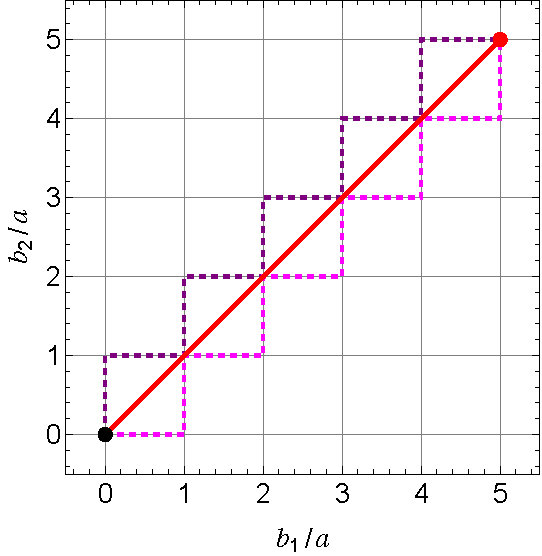
\includegraphics[width=0.85\linewidth]{Example_b_plot_with_2path.pdf}\\
      {\scriptsize Degenerate paths to the same $\vect b$ (solid, dashed) are averaged.}
    \end{column}
    \begin{column}{0.48\textwidth}
      \centering
      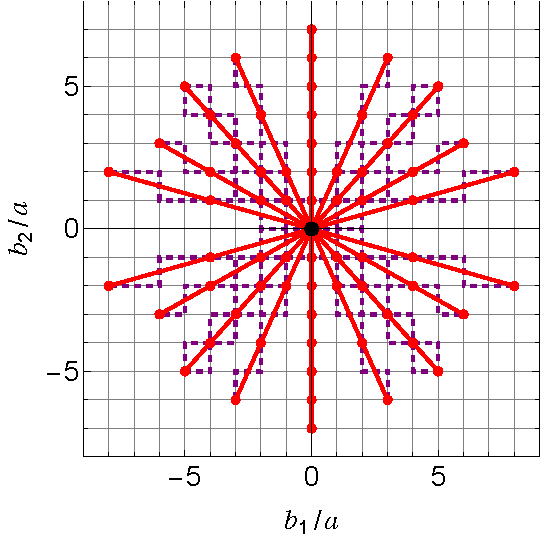
\includegraphics[width=0.85\linewidth]{bL_bT_plot_with_path.pdf}\\
      {\scriptsize Full network: ideal vectors (solid red), averaged staircase paths (dashed)}
    \end{column}
  \end{columns}
  \begin{itemize}
    \item Same operation as for $v$: average over all step-wise paths sharing origin and endpoint.
  \end{itemize}
\end{frame}

% Slide 31
% ===== Correlator decomposition: all four Dirac structures, +b / -b, even / odd (follows thesis, Extracting the x-dependence) =====
\newcommand{\En}{E_N}
\newcommand{\Pa}{|\vec P^{1}|}
\newcommand{\aR}[1]{\tilde a^{\text{Re}}_{#1}}
\newcommand{\aI}[1]{\tilde a^{\text{Im}}_{#1}}
\newcommand{\bR}[1]{\tilde b^{\text{Re}}_{#1}}
\newcommand{\bI}[1]{\tilde b^{\text{Im}}_{#1}}
\newcommand{\Rr}[3]{\text{#1}\{R_{\Gamma(#2)}\}^{[#3]}}
\newcommand{\fl}{\textcolor{red}}

\begin{frame}{Dirac structures $\Gamma$: Euclidean (lattice) versus Minkowski}
  \begin{itemize}
    \item The lattice code uses Euclidean $\gamma_E$; the amplitudes are defined with Minkowski $\gamma_M$:
  \end{itemize}
  \[ \gamma^{1}_{E}=+i\gamma^{1}_{M},\quad \gamma^{2}_{E}=-i\gamma^{2}_{M},\quad \gamma^{3}_{E}=+i\gamma^{3}_{M},\quad \gamma^{4}_{E}=\gamma^{0}_{M},\quad \gamma^{5}_{E}=\gamma^{1}_{E}\gamma^{2}_{E}\gamma^{3}_{E}\gamma^{4}_{E}=-\gamma^{5}_{M} \]
  \begin{itemize}
    \item The index $i\in\{1,2,4,8\}$ of $\Gamma(i)$ is the bit-encoded position of the structure in the CHROMA/QLUA operator basis:
  \end{itemize}
  \[ \Gamma(1)=[+i\gamma^1],\qquad \Gamma(2)=[-i\gamma^2],\qquad \Gamma(4)=[+i\gamma^3],\qquad \Gamma(8)=[\gamma^0] \]
  \begin{itemize}
    \item Measured: the four ratios $R_{\Gamma(1)},R_{\Gamma(2)},R_{\Gamma(4)},R_{\Gamma(8)}$, each complex, at $(+b^1,b^2,0)$ and $(-b^1,b^2,0)$. Raising spatial indices with $g^{\mu\nu}=\mathrm{diag}(1,-1,-1,-1)$ ($P_1=-P^1$, $b_2=-b^2$), and $P^0\to\En$.
    \item Lattice amplitudes (finite link $\eta$): $\tilde a_i=\tilde a_i^{\text{Re}}+i\tilde a_i^{\text{Im}}$, $\tilde b_i=\tilde b_i^{\text{Re}}+i\tilde b_i^{\text{Im}}$, related to the uppercase parametrization by $\tAmp_i=\tilde a_i$, $\tBmp_i=(\eta v\tcdot P)^n\,\tilde b_i$. Here $n=1$ for $i=1,7,8,9$ and $n=2$ for $i=10$.
  \end{itemize}
  \figsrc{Thesis, Extracting the x-dependence, solving real and imaginary amplitudes.}
\end{frame}

\begin{frame}{Lattice geometry and reflection in $b^1$}
  \[
  P^\mu=(\En,-\Pa,0,0),\quad b^\mu=(0,b^1,b^2,0),
  \quad v^\mu=(0,v^1,0,v^3),\quad S^\mu=(0,0,0,1).
  \]
  \[
  b\cdot S=0,\qquad v\cdot S=-v^3,\qquad v\cdot P=\Pa v^1,
  \qquad \epsilon^{0123}=+1.
  \]
  \begin{itemize}
    \item Reflect only $b^1$, keeping $b^2$, $v$, $P$, $S$ and $\eta$ fixed.
    \item Then $b\cdot P$ and $v\cdot b$ both change sign while $b\cdot b$ stays fixed. Hermiticity gives
  \end{itemize}
  \[
  \tilde a_i[-b^1]=\tilde a_i[+b^1]^*,\qquad
  \tilde b_i[-b^1]=\tilde b_i[+b^1]^*.
  \]
  \begin{itemize}
    \item A spatial component $b^2$ in the following equations means the second Cartesian component. It is distinct from the invariant $b\cdot b$ and the magnitude $|\vect b|^2$.
    \item $\tBmp_9$ vanishes in this geometry because $b\cdot S=0$. The other seven amplitudes remain in the four-channel system.
  \end{itemize}
  \figsrc{Thesis, Extracting the x-dependence, lattice kinematics and amplitude inversion.}
\end{frame}

% ---------------- Gamma(8) = gamma^0 ----------------
\begin{frame}{Correlator for $\Gamma(8)=[\gamma^0]$}
  \small
  Continuum projection (contravariant indices, $S^3$ the nucleon polarization):
  \[ \tfrac12\widetilde\Phi^{[\gamma^0]}_{\unsub}=P^0\,\tAmp_2-i\mN\Pa\,\bvec^2S^3\,\tAmp_{12}-\tfrac{i\mN^3}{v\tcdot P}\,\bvec^2v^1S^3\,\tBmp_8-\tfrac{i\mN^3}{(v\tcdot P)^2}(v\tcdot S)\Pa\,\bvec^2v^3\,\tBmp_{10} \]
  Lattice ratio in terms of the finite-link amplitudes:
  \[ R_{\Gamma(8)}=2\Big[\tilde a_2-i\mN\tfrac{\Pa}{\En}\bvec^2\,\tilde a_{12}-\tfrac{i\mN^3}{\En}\bvec^2\eta v^1\,\tilde b_8+\tfrac{i\mN^3}{\En}\Pa\bvec^2\eta^2(v^3)^2\,\tilde b_{10}\Big] \]
  \figsrc{Thesis, Extracting the x-dependence, projected vector correlator.}
\end{frame}

\begin{frame}{$\Gamma(8)$: the $+b^1$ and $-b^1$ equations}
  \small
  \begin{align*}
    \Rr{Re}{8}{+b^1}&=2\Big[\aR2+\mN\tfrac{\Pa}{\En}\bvec^2\aI{12}+\tfrac{\mN^3}{\En}\bvec^2\eta v^1\bI8-\tfrac{\mN^3}{\En}\Pa\bvec^2\eta^2(v^3)^2\bI{10}\Big]\\
    \Rr{Im}{8}{+b^1}&=2\Big[-\mN\tfrac{\Pa}{\En}\bvec^2\aR{12}-\tfrac{\mN^3}{\En}\bvec^2\eta v^1\bR8+\tfrac{\mN^3}{\En}\Pa\bvec^2\eta^2(v^3)^2\bR{10}+\aI2\Big]\\
    \Rr{Re}{8}{-b^1}&=2\Big[\aR2\fl{-}\mN\tfrac{\Pa}{\En}\bvec^2\aI{12}\fl{-}\tfrac{\mN^3}{\En}\bvec^2\eta v^1\bI8\fl{+}\tfrac{\mN^3}{\En}\Pa\bvec^2\eta^2(v^3)^2\bI{10}\Big]\\
    \Rr{Im}{8}{-b^1}&=2\Big[-\mN\tfrac{\Pa}{\En}\bvec^2\aR{12}-\tfrac{\mN^3}{\En}\bvec^2\eta v^1\bR8+\tfrac{\mN^3}{\En}\Pa\bvec^2\eta^2(v^3)^2\bR{10}\fl{-}\aI2\Big]
  \end{align*}
  {\scriptsize Red: sign flipped relative to $+b^1$, because $\tilde a^{\text{Re}},\tilde b^{\text{Re}}$ are even and $\tilde a^{\text{Im}},\tilde b^{\text{Im}}$ are odd in $b^1$ (and $\bvec^1$ itself flips).}
  \figsrc{Thesis, Extracting the x-dependence, solving real and imaginary amplitudes.}
\end{frame}

% ---------------- Gamma(1) = i gamma^1 ----------------
\begin{frame}{Correlator for $\Gamma(1)=[+i\gamma^1]$}
  \small
  Continuum projection:
  \[ \tfrac12\widetilde\Phi^{[\gamma^1]}_{\unsub}=-\Pa\,\tAmp_2-i\mN^2\bvec^1\tAmp_3+\tfrac{\mN^2}{v\tcdot P}v^1\tBmp_1+i\mN P^0\bvec^2S^3\,\tAmp_{12}+\tfrac{i\mN^3}{(v\tcdot P)^2}(v\tcdot S)P^0\bvec^2v^3\,\tBmp_{10} \]
  Lattice ratio:
  \[ R_{\Gamma(1)}=2\Big[-i\tfrac{\Pa}{\En}\tilde a_2+\tfrac{\mN^2}{\En}\bvec^1\tilde a_3+i\tfrac{\mN^2}{\En}\eta v^1\tilde b_1-\mN\bvec^2\tilde a_{12}+\mN^3\bvec^2\eta^2(v^3)^2\tilde b_{10}\Big] \]
  \figsrc{Thesis, Extracting the x-dependence, projected vector correlator.}
\end{frame}

\begin{frame}{$\Gamma(1)$: the $+b^1$ and $-b^1$ equations}
  \small
  \begin{align*}
    \Rr{Re}{1}{+b^1}&=2\Big[\tfrac{\mN^2}{\En}\bvec^1\aR3-\mN\bvec^2\aR{12}+\mN^3\bvec^2\eta^2(v^3)^2\bR{10}+\tfrac{\Pa}{\En}\aI2-\tfrac{\mN^2}{\En}\eta v^1\bI1\Big]\\
    \Rr{Im}{1}{+b^1}&=2\Big[-\tfrac{\Pa}{\En}\aR2+\tfrac{\mN^2}{\En}\eta v^1\bR1+\tfrac{\mN^2}{\En}\bvec^1\aI3-\mN\bvec^2\aI{12}+\mN^3\bvec^2\eta^2(v^3)^2\bI{10}\Big]\\
    \Rr{Re}{1}{-b^1}&=2\Big[\fl{-}\tfrac{\mN^2}{\En}\bvec^1\aR3-\mN\bvec^2\aR{12}+\mN^3\bvec^2\eta^2(v^3)^2\bR{10}\fl{-}\tfrac{\Pa}{\En}\aI2\fl{+}\tfrac{\mN^2}{\En}\eta v^1\bI1\Big]\\
    \Rr{Im}{1}{-b^1}&=2\Big[-\tfrac{\Pa}{\En}\aR2+\tfrac{\mN^2}{\En}\eta v^1\bR1+\tfrac{\mN^2}{\En}\bvec^1\aI3\fl{+}\mN\bvec^2\aI{12}\fl{-}\mN^3\bvec^2\eta^2(v^3)^2\bI{10}\Big]
  \end{align*}
  \figsrc{Thesis, Extracting the x-dependence, solving real and imaginary amplitudes.}
\end{frame}

% ---------------- Gamma(2) = -i gamma^2 ----------------
\begin{frame}{Correlator for $\Gamma(2)=[-i\gamma^2]$}
  \small
  Continuum projection:
  \[ \tfrac12\widetilde\Phi^{[\gamma^2]}_{\unsub}=-i\mN^2\bvec^2\tAmp_3-i\mN P^0\bvec^1S^3\,\tAmp_{12}+\tfrac{\mN}{v\tcdot P}P^0v^1S^3\,\tBmp_7-\tfrac{i\mN^3}{(v\tcdot P)^2}(v\tcdot S)P^0\bvec^1v^3\,\tBmp_{10} \]
  Lattice ratio:
  \[ R_{\Gamma(2)}=2\Big[-\tfrac{\mN^2}{\En}\bvec^2\tilde a_3-\mN\bvec^1\tilde a_{12}-i\mN\eta v^1\tilde b_7+\mN^3\bvec^1\eta^2(v^3)^2\tilde b_{10}\Big] \]
  \figsrc{Thesis, Extracting the x-dependence, projected vector correlator.}
\end{frame}

\begin{frame}{$\Gamma(2)$: the $+b^1$ and $-b^1$ equations}
  \small
  \begin{align*}
    \Rr{Re}{2}{+b^1}&=2\Big[-\tfrac{\mN^2}{\En}\bvec^2\aR3-\mN\bvec^1\aR{12}+\mN^3\bvec^1\eta^2(v^3)^2\bR{10}+\mN\eta v^1\bI7\Big]\\
    \Rr{Im}{2}{+b^1}&=2\Big[-\mN\eta v^1\bR7-\tfrac{\mN^2}{\En}\bvec^2\aI3-\mN\bvec^1\aI{12}+\mN^3\bvec^1\eta^2(v^3)^2\bI{10}\Big]\\
    \Rr{Re}{2}{-b^1}&=2\Big[-\tfrac{\mN^2}{\En}\bvec^2\aR3\fl{+}\mN\bvec^1\aR{12}\fl{-}\mN^3\bvec^1\eta^2(v^3)^2\bR{10}\fl{-}\mN\eta v^1\bI7\Big]\\
    \Rr{Im}{2}{-b^1}&=2\Big[-\mN\eta v^1\bR7\fl{+}\tfrac{\mN^2}{\En}\bvec^2\aI3-\mN\bvec^1\aI{12}+\mN^3\bvec^1\eta^2(v^3)^2\bI{10}\Big]
  \end{align*}
  \figsrc{Thesis, Extracting the x-dependence, solving real and imaginary amplitudes.}
\end{frame}

% ---------------- Gamma(4) = i gamma^3 ----------------
\begin{frame}{Correlator for $\Gamma(4)=[+i\gamma^3]$}
  \small
  Continuum projection:
  \[ \tfrac12\widetilde\Phi^{[\gamma^3]}_{\unsub}=\tfrac{\mN^2}{v\tcdot P}v^3\,\tBmp_1-\tfrac{i\mN^3}{(v\tcdot P)^2}(v\tcdot S)P^0\bvec^2v^1\,\tBmp_{10} \]
  Lattice ratio:
  \[ R_{\Gamma(4)}=2\Big[i\tfrac{\mN^2}{\En}\eta v^3\tilde b_1-\mN^3\bvec^2\eta^2v^1v^3\,\tilde b_{10}\Big] \]
  \figsrc{Thesis, Extracting the x-dependence, projected vector correlator.}
\end{frame}

\begin{frame}{$\Gamma(4)$: the $+b^1$ and $-b^1$ equations}
  \small
  \begin{align*}
    \Rr{Re}{4}{+b^1}&=2\Big[-\mN^3\bvec^2\eta^2v^1v^3\bR{10}-\tfrac{\mN^2}{\En}\eta v^3\bI1\Big]\\
    \Rr{Im}{4}{+b^1}&=2\Big[\tfrac{\mN^2}{\En}\eta v^3\bR1-\mN^3\bvec^2\eta^2v^1v^3\bI{10}\Big]\\
    \Rr{Re}{4}{-b^1}&=2\Big[-\mN^3\bvec^2\eta^2v^1v^3\bR{10}\fl{+}\tfrac{\mN^2}{\En}\eta v^3\bI1\Big]\\
    \Rr{Im}{4}{-b^1}&=2\Big[\tfrac{\mN^2}{\En}\eta v^3\bR1\fl{+}\mN^3\bvec^2\eta^2v^1v^3\bI{10}\Big]
  \end{align*}
  \figsrc{Thesis, Extracting the x-dependence, solving real and imaginary amplitudes.}
\end{frame}

\begin{frame}{Matrix construction: coefficient definitions}
  \small
  To display both reflections side by side, define the exact coefficients
  \begin{align*}
    p&=\frac{\Pa}{\En},&u_1&=\frac{\mN^2b^1}{\En},&u_2&=\frac{\mN^2b^2}{\En},\\
    s_1&=\mN b^1,&s_2&=\mN b^2,&h&=\mN\eta v^1,\\
    \ell_1&=\frac{\mN^2\eta v^1}{\En},&\ell_3&=\frac{\mN^2\eta v^3}{\En},&k&=\frac{\mN^3b^2\eta v^1}{\En},\\
    t_1&=\mN^3b^1\eta^2(v^3)^2,&t_2&=\mN^3b^2\eta^2(v^3)^2,&w&=\mN^3b^2\eta^2v^1v^3.
  \end{align*}
  \[
  \boldsymbol R_\pm=
   (R_{\Gamma(1)}^{[\pm b^1]},R_{\Gamma(2)}^{[\pm b^1]},
    R_{\Gamma(4)}^{[\pm b^1]},R_{\Gamma(8)}^{[\pm b^1]})^{\mathsf T}.
  \]
  \[
  \boldsymbol a_+=(\tilde a_2,\tilde a_3,\tilde a_{12})^{\mathsf T},\quad
  \boldsymbol b_+=(\tilde b_1,\tilde b_7,\tilde b_8,\tilde b_{10})^{\mathsf T},\quad
  \boldsymbol a_-=\boldsymbol a_+^*,\quad\boldsymbol b_-=\boldsymbol b_+^*.
  \]
  \figsrc{Algebraic matrix form of the four thesis ratio equations. Coefficients refer to $+b^1$.}
\end{frame}

\begin{frame}{The $+b^1$ and $-b^1$ matrices: $a$ amplitudes}
  \[
    \frac{\boldsymbol R_\pm}{2}
       =M_{a,\pm}\boldsymbol a_\pm+M_{b,\pm}\boldsymbol b_\pm.
  \]
  \begin{columns}[c]
    \begin{column}{.49\textwidth}
      \[M_{a,+}=\begin{pmatrix}
       -ip&u_1&-s_2\\
       0&-u_2&-s_1\\
       0&0&0\\
       1&0&-ip s_2
      \end{pmatrix}.\]
    \end{column}
    \begin{column}{.49\textwidth}
      \[M_{a,-}=\begin{pmatrix}
       -ip&-u_1&-s_2\\
       0&-u_2&+s_1\\
       0&0&0\\
       1&0&-ip s_2
      \end{pmatrix}.\]
    \end{column}
  \end{columns}
  \begin{itemize}
    \item Columns: $(\tilde a_2,\tilde a_3,\tilde a_{12})$. Rows: $\Gamma(1),\Gamma(2),\Gamma(4),\Gamma(8)$.
    \item The entries proportional to $b^1$ change sign. Separately, the imaginary parts of all amplitudes change sign through $\boldsymbol a_-=\boldsymbol a_+^*$.
    \item The complete $b$-amplitude contribution is displayed on the next slide.
  \end{itemize}
  \figsrc{Thesis, Extracting the x-dependence, full $\pm b^1$ correlator system.}
\end{frame}

\begin{frame}{The $+b^1$ and $-b^1$ matrices: $b$ amplitudes}
  \[
    \frac{\boldsymbol R_\pm}{2}
       =M_{a,\pm}\boldsymbol a_\pm+M_{b,\pm}\boldsymbol b_\pm.
  \]
  \begin{columns}[c]
    \begin{column}{.49\textwidth}
      \[M_{b,+}=\begin{pmatrix}
       i\ell_1&0&0&t_2\\
       0&-ih&0&t_1\\
       i\ell_3&0&0&-w\\
       0&0&-ik&ip t_2
      \end{pmatrix}.\]
    \end{column}
    \begin{column}{.49\textwidth}
      \[M_{b,-}=\begin{pmatrix}
       i\ell_1&0&0&t_2\\
       0&-ih&0&-t_1\\
       i\ell_3&0&0&-w\\
       0&0&-ik&ip t_2
      \end{pmatrix}.\]
    \end{column}
  \end{columns}
  \begin{itemize}
    \item Columns: $(\tilde b_1,\tilde b_7,\tilde b_8,\tilde b_{10})$. Row order is unchanged.
    \item Only $t_1\propto b^1$ changes sign in these coefficient matrices.
    \item Combine the two matrix blocks before taking even and odd projections. No tensor structures have been dropped from this geometry.
  \end{itemize}
  \figsrc{Thesis, Extracting the x-dependence, full $\pm b^1$ correlator system.}
\end{frame}

\begin{frame}{Even and odd projections of the full system}
  \[
    \boldsymbol R_{\rm e}=\frac{\boldsymbol R_++\boldsymbol R_-}{2},
    \qquad\boldsymbol R_{\rm o}=\frac{\boldsymbol R_+-\boldsymbol R_-}{2}.
  \]
  For either block $M=M_a$ or $M_b$, set
  $M_{\rm e}=(M_++M_-)/2$ and $M_{\rm o}=(M_+-M_-)/2$. Then
  \begin{align*}
  \frac{\boldsymbol R_{\rm e}}2
    &=M_{a,\rm e}\Re\boldsymbol a_+
       +iM_{a,\rm o}\Im\boldsymbol a_+
       +M_{b,\rm e}\Re\boldsymbol b_+
       +iM_{b,\rm o}\Im\boldsymbol b_+,\\
  \frac{\boldsymbol R_{\rm o}}2
    &=M_{a,\rm o}\Re\boldsymbol a_+
       +iM_{a,\rm e}\Im\boldsymbol a_+
       +M_{b,\rm o}\Re\boldsymbol b_+
       +iM_{b,\rm e}\Im\boldsymbol b_+.
  \end{align*}
  \begin{itemize}
    \item Matrix parity and amplitude parity both matter. An even ratio can contain $b^1\tilde a_i^{\rm Im}$ because both factors are odd.
    \item The following slides expand every real and imaginary component of these two equations.
  \end{itemize}
  \figsrc{Direct sum and difference of the full $\pm b^1$ systems in the thesis.}
\end{frame}

% ---------------- even combination ----------------
\begin{frame}{$b^1$-even projection $\tfrac12(R^{[+b^1]}+R^{[-b^1]})$: $\Gamma(1),\Gamma(2)$}
  \small
  \begin{align*}
    \Rr{Re}{1}{b^1\text{-even}}&=2\Big[-\mN\bvec^2\aR{12}+\mN^3\bvec^2\eta^2(v^3)^2\bR{10}\Big]\\
    \Rr{Im}{1}{b^1\text{-even}}&=2\Big[-\tfrac{\Pa}{\En}\aR2+\tfrac{\mN^2}{\En}\eta v^1\bR1+\tfrac{\mN^2}{\En}\bvec^1\aI3\Big]\\
    \Rr{Re}{2}{b^1\text{-even}}&=2\Big[-\tfrac{\mN^2}{\En}\bvec^2\aR3\Big]\\
    \Rr{Im}{2}{b^1\text{-even}}&=2\Big[-\mN\eta v^1\bR7-\mN\bvec^1\aI{12}+\mN^3\bvec^1\eta^2(v^3)^2\bI{10}\Big]
  \end{align*}
  \begin{itemize}
    \item The even projection keeps $\tilde a^{\text{Re}}$, $\tilde b^{\text{Re}}$ and the products $\bvec^1\tilde a^{\text{Im}}$, $\bvec^1\tilde b^{\text{Im}}$.
  \end{itemize}
  \figsrc{Thesis, Extracting the x-dependence, solving real and imaginary amplitudes.}
\end{frame}

\begin{frame}{$b^1$-even projection $\tfrac12(R^{[+b^1]}+R^{[-b^1]})$: $\Gamma(4),\Gamma(8)$}
  \small
  \begin{align*}
    \Rr{Re}{4}{b^1\text{-even}}&=2\Big[-\mN^3\bvec^2\eta^2v^1v^3\bR{10}\Big]\\
    \Rr{Im}{4}{b^1\text{-even}}&=2\Big[\tfrac{\mN^2}{\En}\eta v^3\bR1\Big]\\
    \Rr{Re}{8}{b^1\text{-even}}&=2\Big[\aR2\Big]\\
    \Rr{Im}{8}{b^1\text{-even}}&=2\Big[-\mN\tfrac{\Pa}{\En}\bvec^2\aR{12}-\tfrac{\mN^3}{\En}\bvec^2\eta v^1\bR8+\tfrac{\mN^3}{\En}\Pa\bvec^2\eta^2(v^3)^2\bR{10}\Big]
  \end{align*}
  \figsrc{Thesis, Extracting the x-dependence, solving real and imaginary amplitudes.}
\end{frame}

% ---------------- odd combination ----------------
\begin{frame}{$b^1$-odd projection $\tfrac12(R^{[+b^1]}-R^{[-b^1]})$: $\Gamma(1),\Gamma(2)$}
  \small
  \begin{align*}
    \Rr{Re}{1}{b^1\text{-odd}}&=2\Big[\tfrac{\mN^2}{\En}\bvec^1\aR3+\tfrac{\Pa}{\En}\aI2-\tfrac{\mN^2}{\En}\eta v^1\bI1\Big]\\
    \Rr{Im}{1}{b^1\text{-odd}}&=2\Big[-\mN\bvec^2\aI{12}+\mN^3\bvec^2\eta^2(v^3)^2\bI{10}\Big]\\
    \Rr{Re}{2}{b^1\text{-odd}}&=2\Big[-\mN\bvec^1\aR{12}+\mN^3\bvec^1\eta^2(v^3)^2\bR{10}+\mN\eta v^1\bI7\Big]\\
    \Rr{Im}{2}{b^1\text{-odd}}&=2\Big[-\tfrac{\mN^2}{\En}\bvec^2\aI3\Big]
  \end{align*}
  \figsrc{Thesis, Extracting the x-dependence, solving real and imaginary amplitudes.}
\end{frame}

\begin{frame}{$b^1$-odd projection $\tfrac12(R^{[+b^1]}-R^{[-b^1]})$: $\Gamma(4),\Gamma(8)$}
  \small
  \begin{align*}
    \Rr{Re}{4}{b^1\text{-odd}}&=2\Big[-\tfrac{\mN^2}{\En}\eta v^3\bI1\Big]\\
    \Rr{Im}{4}{b^1\text{-odd}}&=2\Big[-\mN^3\bvec^2\eta^2v^1v^3\bI{10}\Big]\\
    \Rr{Re}{8}{b^1\text{-odd}}&=2\Big[\mN\tfrac{\Pa}{\En}\bvec^2\aI{12}+\tfrac{\mN^3}{\En}\bvec^2\eta v^1\bI8-\tfrac{\mN^3}{\En}\Pa\bvec^2\eta^2(v^3)^2\bI{10}\Big]\\
    \Rr{Im}{8}{b^1\text{-odd}}&=2\Big[\aI2\Big]
  \end{align*}
  \figsrc{Thesis, Extracting the x-dependence, solving real and imaginary amplitudes.}
\end{frame}

\begin{frame}{Real amplitudes from the even system}
  \normalsize

      \begin{align*}
        \aR2&=\tfrac12\Rr{Re}{8}{b^1\text{-even}}\\
        \bR1&=\tfrac{\En}{2\mN^2\eta v^3}\Rr{Im}{4}{b^1\text{-even}}\\
        \aR{12}&=\tfrac{-1}{2\mN\bvec^2}\Big[\Rr{Re}{1}{b^1\text{-even}}\\&\quad+\tfrac{v^3}{v^1}\Rr{Re}{4}{b^1\text{-even}}\Big]\\
        \bR8&=\tfrac{-\En}{2\mN^3\bvec^2\eta v^1}\Big[\Rr{Im}{8}{b^1\text{-even}}\\&\quad+\tfrac{\Pa v^3}{\En v^1}\Rr{Re}{4}{b^1\text{-even}}\\&\quad+2\mN\tfrac{\Pa}{\En}\bvec^2\aR{12}\Big]
      \end{align*}
  \figsrc{Thesis, Extracting the x-dependence, amplitude inversion.}
\end{frame}

\begin{frame}{Imaginary amplitudes from the odd system}
  \normalsize

      \begin{align*}
        \aI2&=\tfrac12\Rr{Im}{8}{b^1\text{-odd}}\\
        \bI1&=\tfrac{-\En}{2\mN^2\eta v^3}\Rr{Re}{4}{b^1\text{-odd}}\\
        \aI{12}&=\tfrac{-1}{2\mN\bvec^2}\Big[\Rr{Im}{1}{b^1\text{-odd}}\\&\quad+\tfrac{v^3}{v^1}\Rr{Im}{4}{b^1\text{-odd}}\Big]\\
        \bI8&=\tfrac{\En}{2\mN^3\bvec^2\eta v^1}\Big[\Rr{Re}{8}{b^1\text{-odd}}\\&\quad-\tfrac{\Pa v^3}{\En v^1}\Rr{Im}{4}{b^1\text{-odd}}\\&\quad-2\mN\tfrac{\Pa}{\En}\bvec^2\aI{12}\Big]
      \end{align*}
  \figsrc{Thesis, Extracting the x-dependence, amplitude inversion.}
\end{frame}

\begin{frame}{Uppercase amplitudes and the staple-length factors}
  \small
  For the Sivers-relevant amplitudes, $v\cdot P=\Pa v^1$ gives
  \[
    \tAmp_2=\tilde a_2,\qquad \tAmp_{12}=\tilde a_{12},\qquad
    \tBmp_1=\eta\Pa v^1\tilde b_1,\qquad
    \tBmp_8=\eta\Pa v^1\tilde b_8.
  \]
  In particular, multiplication by $\eta v\cdot P$ cancels $\eta$ in both parts of $\tBmp_1$:
  \begin{align*}
    \tBmp_1^{\rm Re}&=\frac{\En\Pa v^1}{2\mN^2v^3}
       \Rr{Im}{4}{b^1\text{-even}},\\
    \tBmp_1^{\rm Im}&=-\frac{\En\Pa v^1}{2\mN^2v^3}
       \Rr{Re}{4}{b^1\text{-odd}}.
  \end{align*}
  \[
   \tAmp_{2B}=\tAmp_2+R(\zetahat^2)\tBmp_1,\qquad
   \tAmp_{12B}=\tAmp_{12}-R(\zetahat^2)\tBmp_8.
  \]
  The componentwise inversions assume $b^2\ne0$, $\eta v^1\ne0$ and $\eta v^3\ne0$.
  At singular geometries, use the original correlator system and its symmetry limits.
  \figsrc{Thesis amplitude mapping, with the $\eta$ cancellation applied consistently to both real and imaginary parts.}
\end{frame}


\begin{frame}{Effective amplitudes and invariant coordinates}
  The extracted primitive amplitudes form the combinations
  \begin{align*}
    \tAmp_{2B}^{\mathrm{Re}}&=\tAmp_2^{\mathrm{Re}}+R(\zetahat^2)\tBmp_1^{\mathrm{Re}},&
    \tAmp_{2B}^{\mathrm{Im}}&=\tAmp_2^{\mathrm{Im}}+R(\zetahat^2)\tBmp_1^{\mathrm{Im}},\\
    \tAmp_{12B}^{\mathrm{Re}}&=\tAmp_{12}^{\mathrm{Re}}-R(\zetahat^2)\tBmp_8^{\mathrm{Re}},&
    \tAmp_{12B}^{\mathrm{Im}}&=\tAmp_{12}^{\mathrm{Im}}-R(\zetahat^2)\tBmp_8^{\mathrm{Im}}.
  \end{align*}
  \[ R(\zetahat^2)=1-\sqrt{1+\zetahat^{-2}},\qquad
     \nu=-p_L b_L,\quad s=b_L^2+b_T^2,\quad
     b_L=-\frac{\nu}{p_L},\quad b_T^2=s-\frac{\nu^2}{p_L^2}. \]
  \begin{itemize}
    \item Here $p_L=2\pi P_L/(a\hat L)$ is the physical momentum; $P_L\in\{-1,-2,-3,-4\}$ labels the lattice momentum mode.
    \item $b^{(2)}=b_T$ is a spatial component. It is distinct from the positive squared distance $s$, often denoted $b^2$ in the plots.
    \item The extraction divides by $b^{(2)}$, while the fitted radial denominator uses $s$.
  \end{itemize}
  \figsrc{Thesis, Ch. 5: effective amplitudes and Lorentz-invariant mapping; component notation made explicit.}
\end{frame}

\begin{frame}{The Fourier integral extends beyond the measured domain}
  \[ b_T^2=s-\frac{\nu^2}{p_L^2}\ge0
      \quad\Longrightarrow\quad |\nu|\le |p_L|\sqrt{s}
      \quad\text{for real spatial lattice separations}. \]
  \begin{itemize}
    \item The measured points occupy a finite, irregular subset of this domain.
    \item The Fourier integral requires all real $\nu$ at fixed $s$. A fitted function therefore extends the amplitude beyond the directly sampled region.
    \item Decay of a fit along $b_L$ at fixed lattice $b_T$ does not by itself ensure integrability in $\nu$ at fixed $s$.
    \item Candidate selection must test the transformed model, its tails, and its resulting $x$-dependence as well as its fit quality.
  \end{itemize}
  \figsrc{Thesis, Chs. 5--6: invariant mapping and Fourier-integrability requirement.}
\end{frame}

\begin{frame}{Raw amplitude profiles at all four momenta}
  \begin{itemize}
    \item The following figures show every raw-amplitude view used in the thesis, before fitting.
    \item For each momentum, retain all four components: $\tAmp_{2B}^{\mathrm{Re}}$, $\tAmp_{2B}^{\mathrm{Im}}$, $\tAmp_{12B}^{\mathrm{Re}}$, $\tAmp_{12B}^{\mathrm{Im}}$.
    \item Each component is displayed in lattice coordinates and invariant coordinates, both as a surface and at $\eta|v|/a=8$.
    \item The two panels of each original figure show complementary coordinate slices or views. Both are retained.
  \end{itemize}
  \figsrc{Thesis, Ch. 5: numerical results and parity constraints.}
\end{frame}

\begin{frame}{$\tAmp_{2B}^{\mathrm{Re}}$ at $P_L=-1$: lattice coordinates}
\centering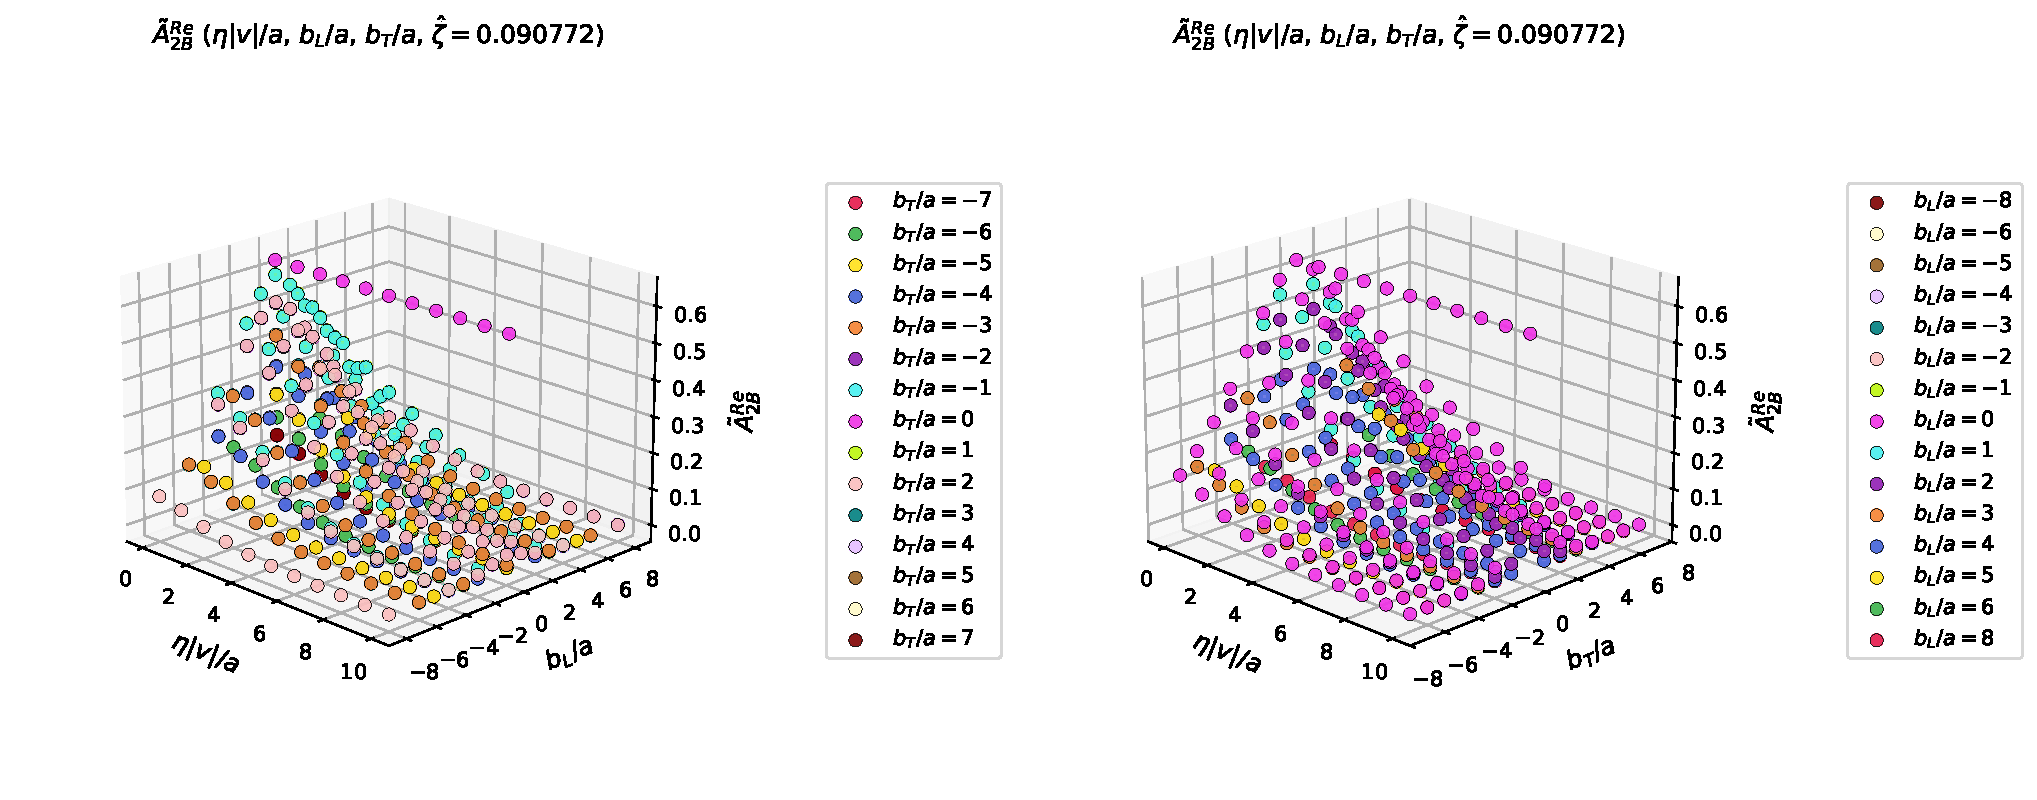
\includegraphics[width=0.98\linewidth,height=0.73\textheight,keepaspectratio]{ReA2B_PL-1_3D.pdf}\\[1mm]
{\small $\zetahat=0.090772$; $(b_L,b_T)$; staple-length dependence}
\figsrc{Thesis, Ch. 5: raw amplitude profiles; complete original panels.}
\end{frame}

\begin{frame}{$\tAmp_{2B}^{\mathrm{Re}}$ at $P_L=-1$: invariant coordinates}
\centering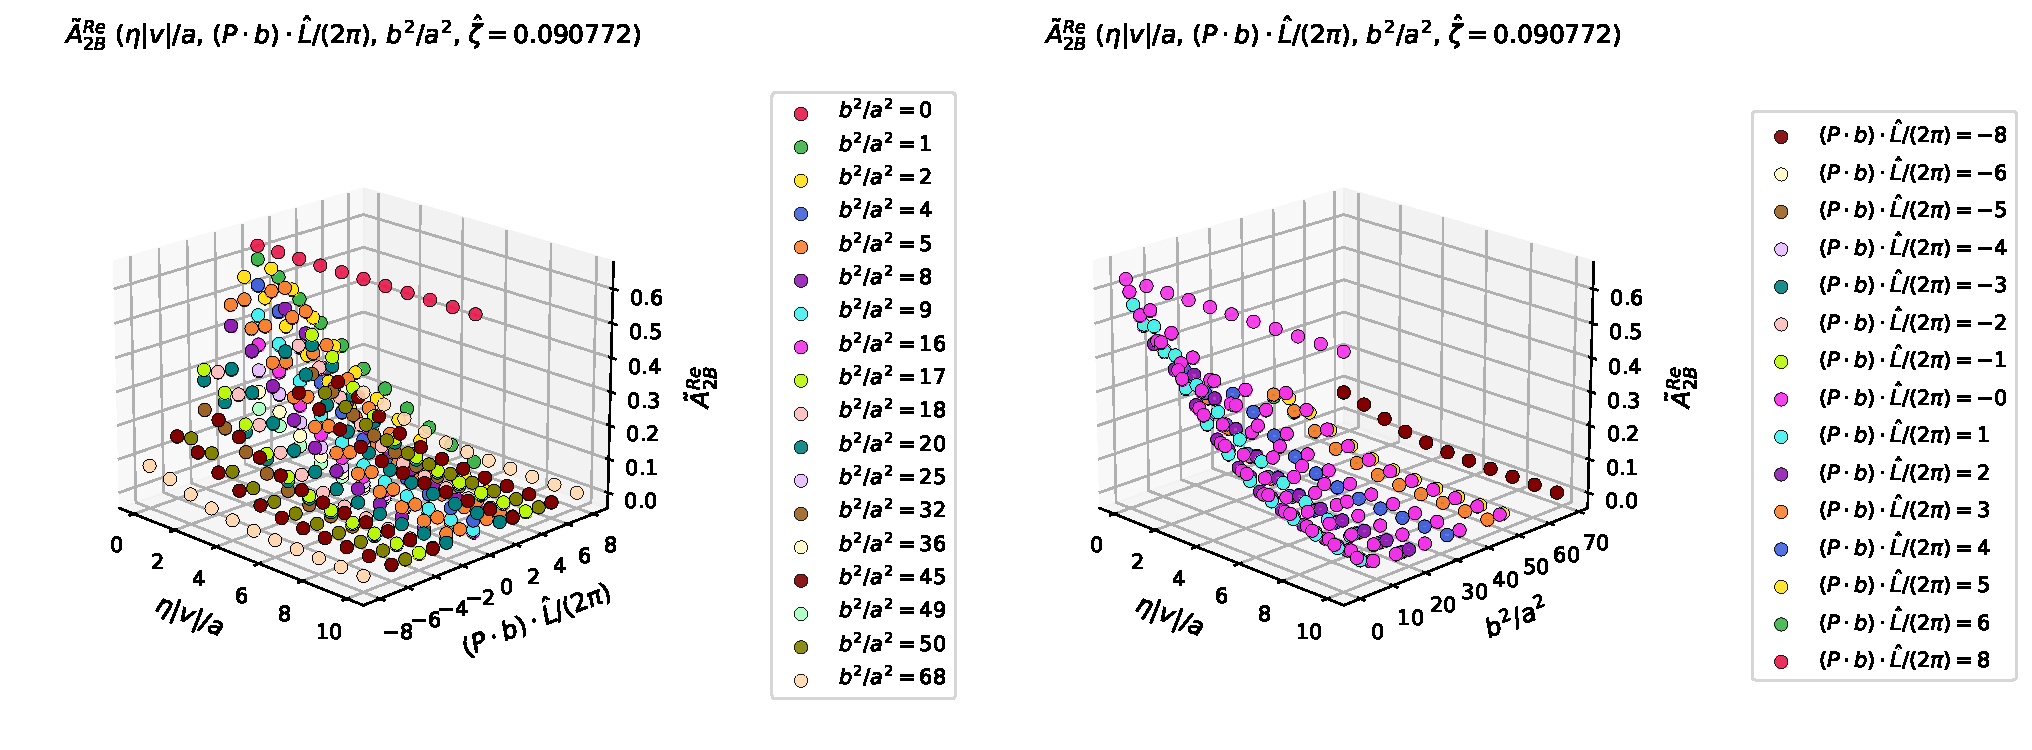
\includegraphics[width=0.98\linewidth,height=0.73\textheight,keepaspectratio]{ReA2B_Pb_bsq_PL-1_3D.pdf}\\[1mm]
{\small $\zetahat=0.090772$; $(\nu,s)$; staple-length dependence}
\figsrc{Thesis, Ch. 5: raw amplitude profiles; complete original panels.}
\end{frame}

\begin{frame}{$\tAmp_{2B}^{\mathrm{Im}}$ at $P_L=-1$: lattice coordinates}
\centering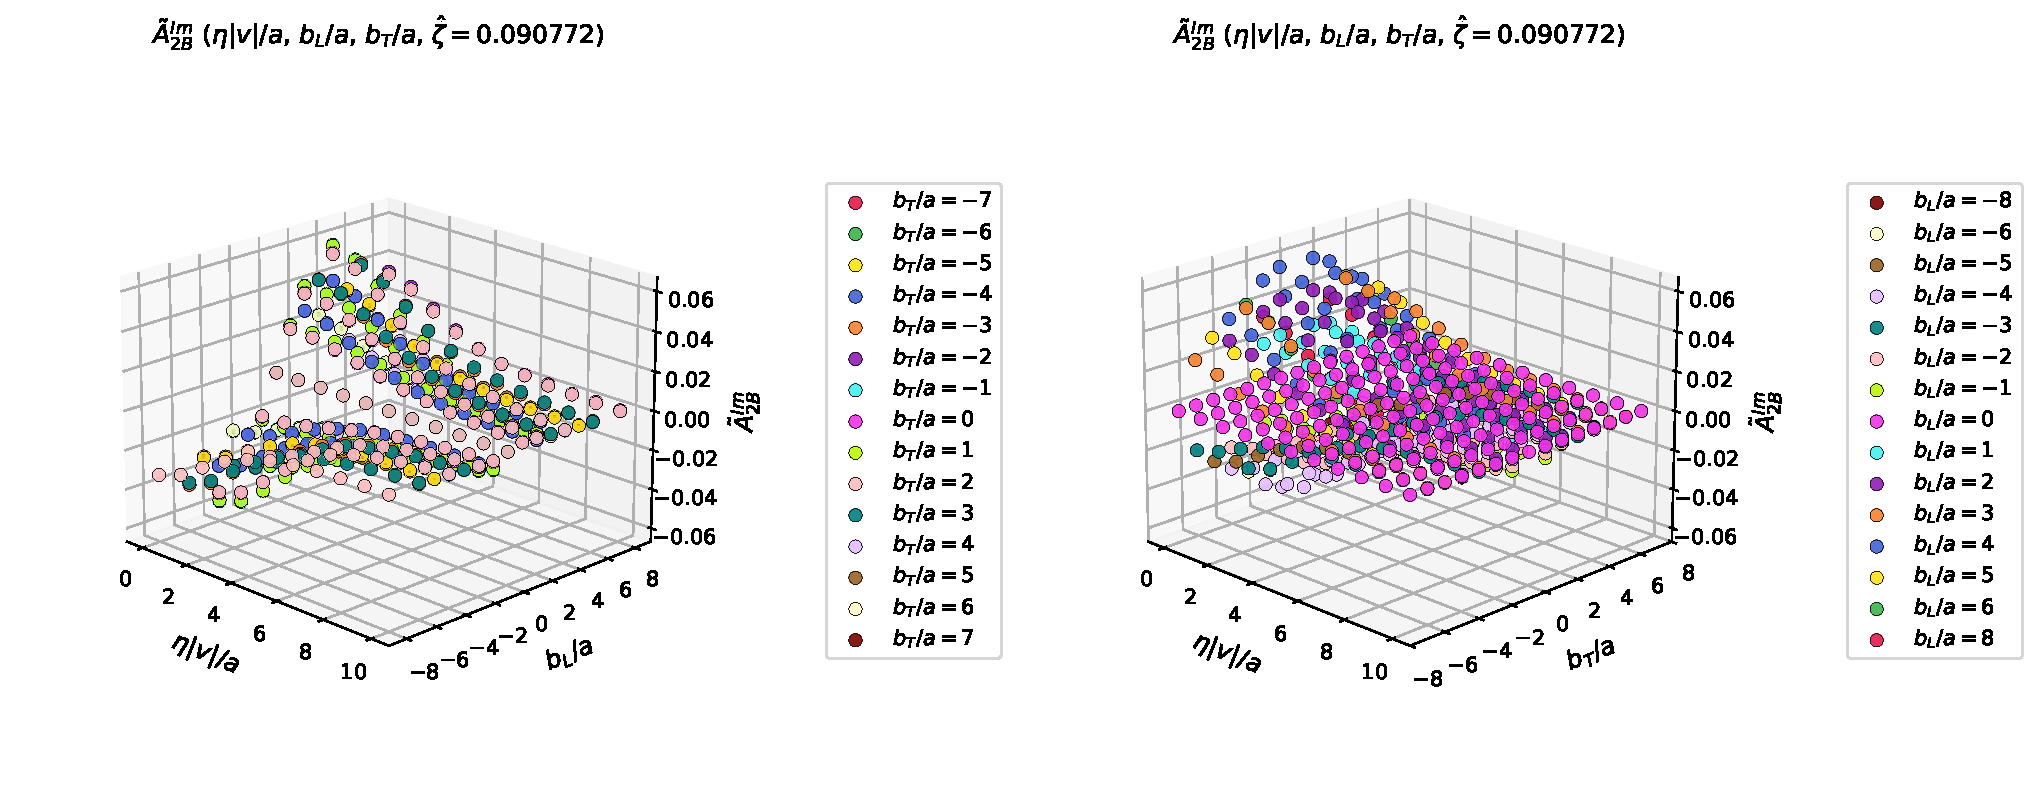
\includegraphics[width=0.98\linewidth,height=0.73\textheight,keepaspectratio]{ImA2B_PL-1_3D.pdf}\\[1mm]
{\small $\zetahat=0.090772$; $(b_L,b_T)$; staple-length dependence}
\figsrc{Thesis, Ch. 5: raw amplitude profiles; complete original panels.}
\end{frame}

\begin{frame}{$\tAmp_{2B}^{\mathrm{Im}}$ at $P_L=-1$: invariant coordinates}
\centering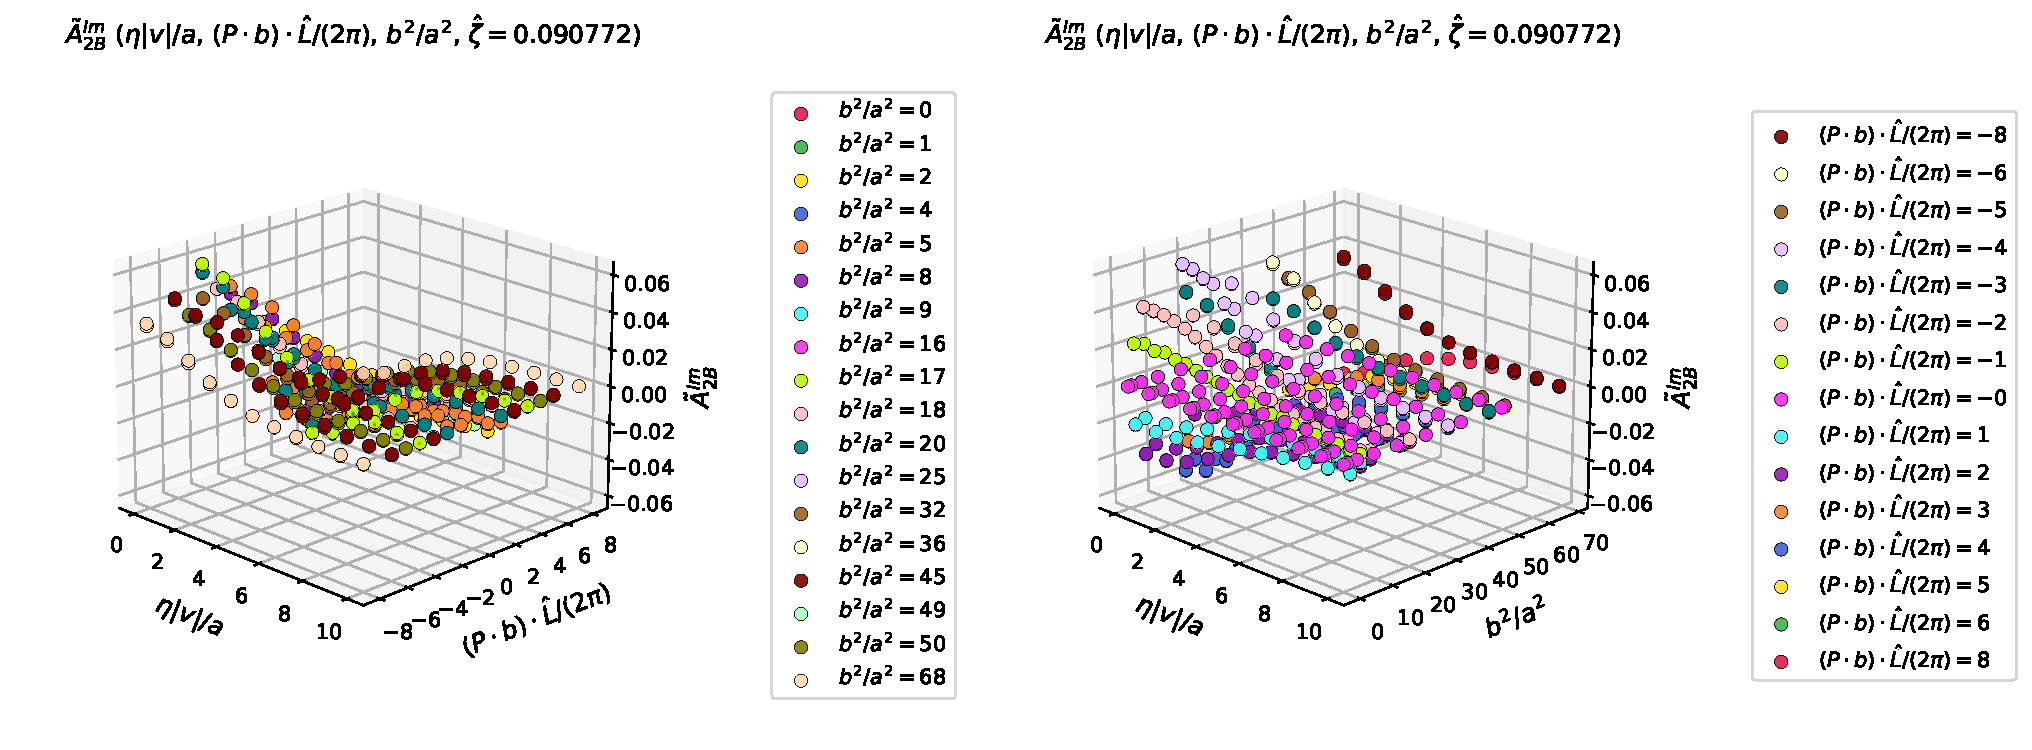
\includegraphics[width=0.98\linewidth,height=0.73\textheight,keepaspectratio]{ImA2B_Pb_bsq_PL-1_3D.pdf}\\[1mm]
{\small $\zetahat=0.090772$; $(\nu,s)$; staple-length dependence}
\figsrc{Thesis, Ch. 5: raw amplitude profiles; complete original panels.}
\end{frame}

\begin{frame}{$\tAmp_{12B}^{\mathrm{Re}}$ at $P_L=-1$: lattice coordinates}
\centering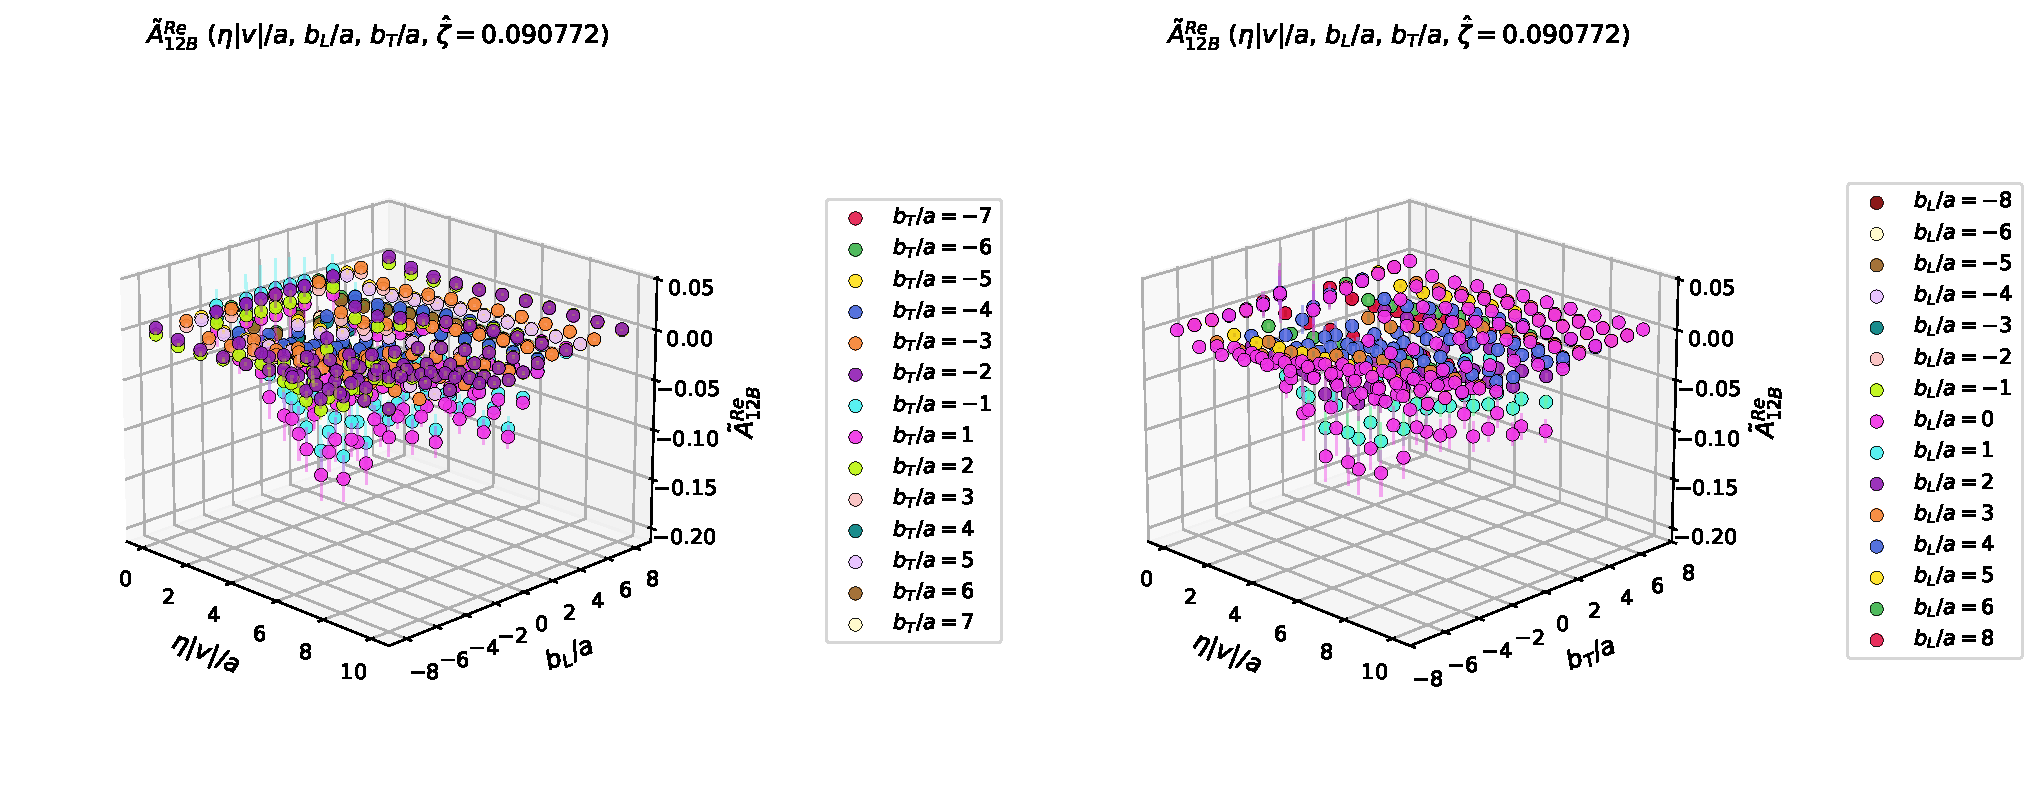
\includegraphics[width=0.98\linewidth,height=0.73\textheight,keepaspectratio]{ReA12B_PL-1_3D.pdf}\\[1mm]
{\small $\zetahat=0.090772$; $(b_L,b_T)$; staple-length dependence}
\figsrc{Thesis, Ch. 5: raw amplitude profiles; complete original panels.}
\end{frame}

\begin{frame}{$\tAmp_{12B}^{\mathrm{Re}}$ at $P_L=-1$: invariant coordinates}
\centering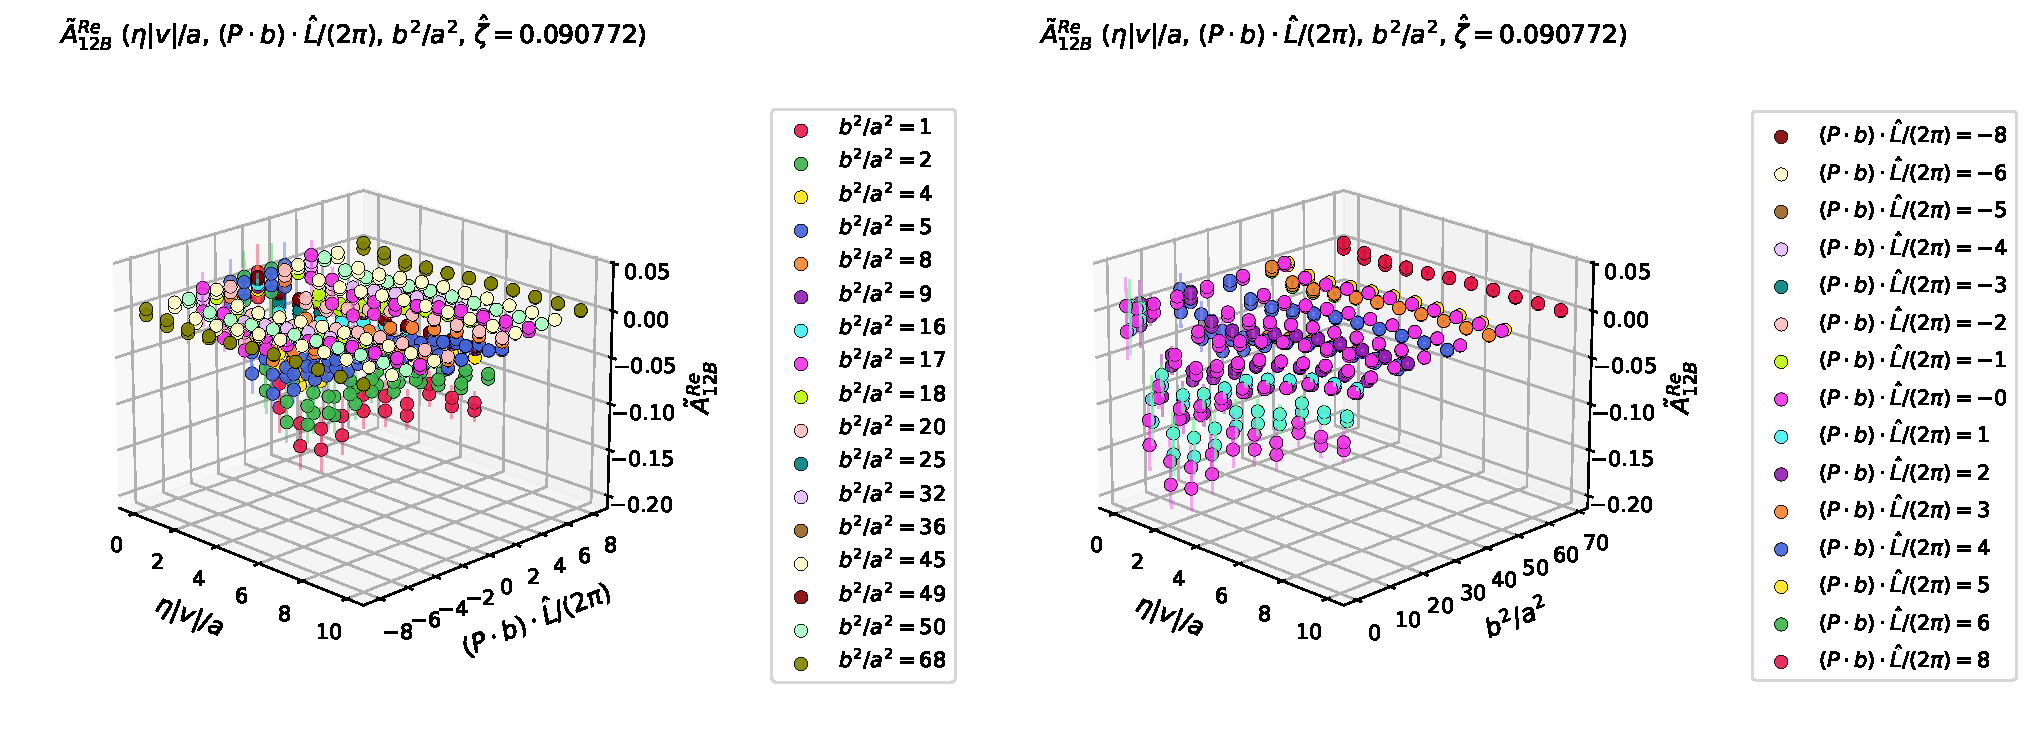
\includegraphics[width=0.98\linewidth,height=0.73\textheight,keepaspectratio]{ReA12B_Pb_bsq_PL-1_3D.pdf}\\[1mm]
{\small $\zetahat=0.090772$; $(\nu,s)$; staple-length dependence}
\figsrc{Thesis, Ch. 5: raw amplitude profiles; complete original panels.}
\end{frame}

\begin{frame}{$\tAmp_{12B}^{\mathrm{Im}}$ at $P_L=-1$: lattice coordinates}
\centering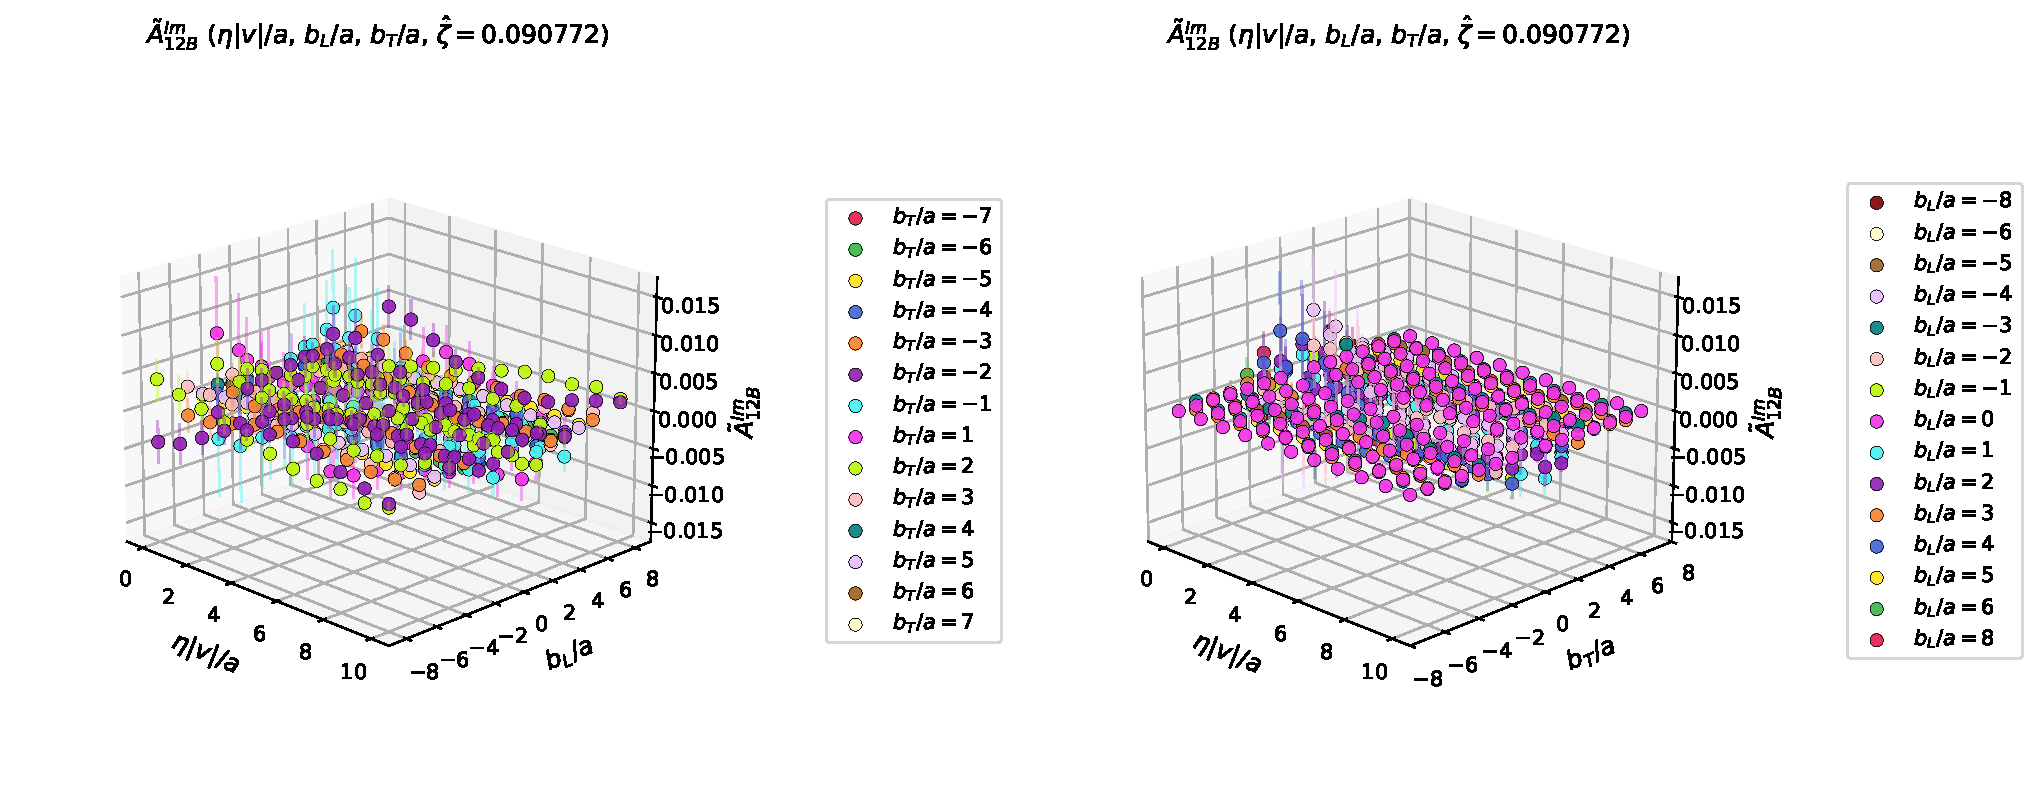
\includegraphics[width=0.98\linewidth,height=0.73\textheight,keepaspectratio]{ImA12B_PL-1_3D.pdf}\\[1mm]
{\small $\zetahat=0.090772$; $(b_L,b_T)$; staple-length dependence}
\figsrc{Thesis, Ch. 5: raw amplitude profiles; complete original panels.}
\end{frame}

\begin{frame}{$\tAmp_{12B}^{\mathrm{Im}}$ at $P_L=-1$: invariant coordinates}
\centering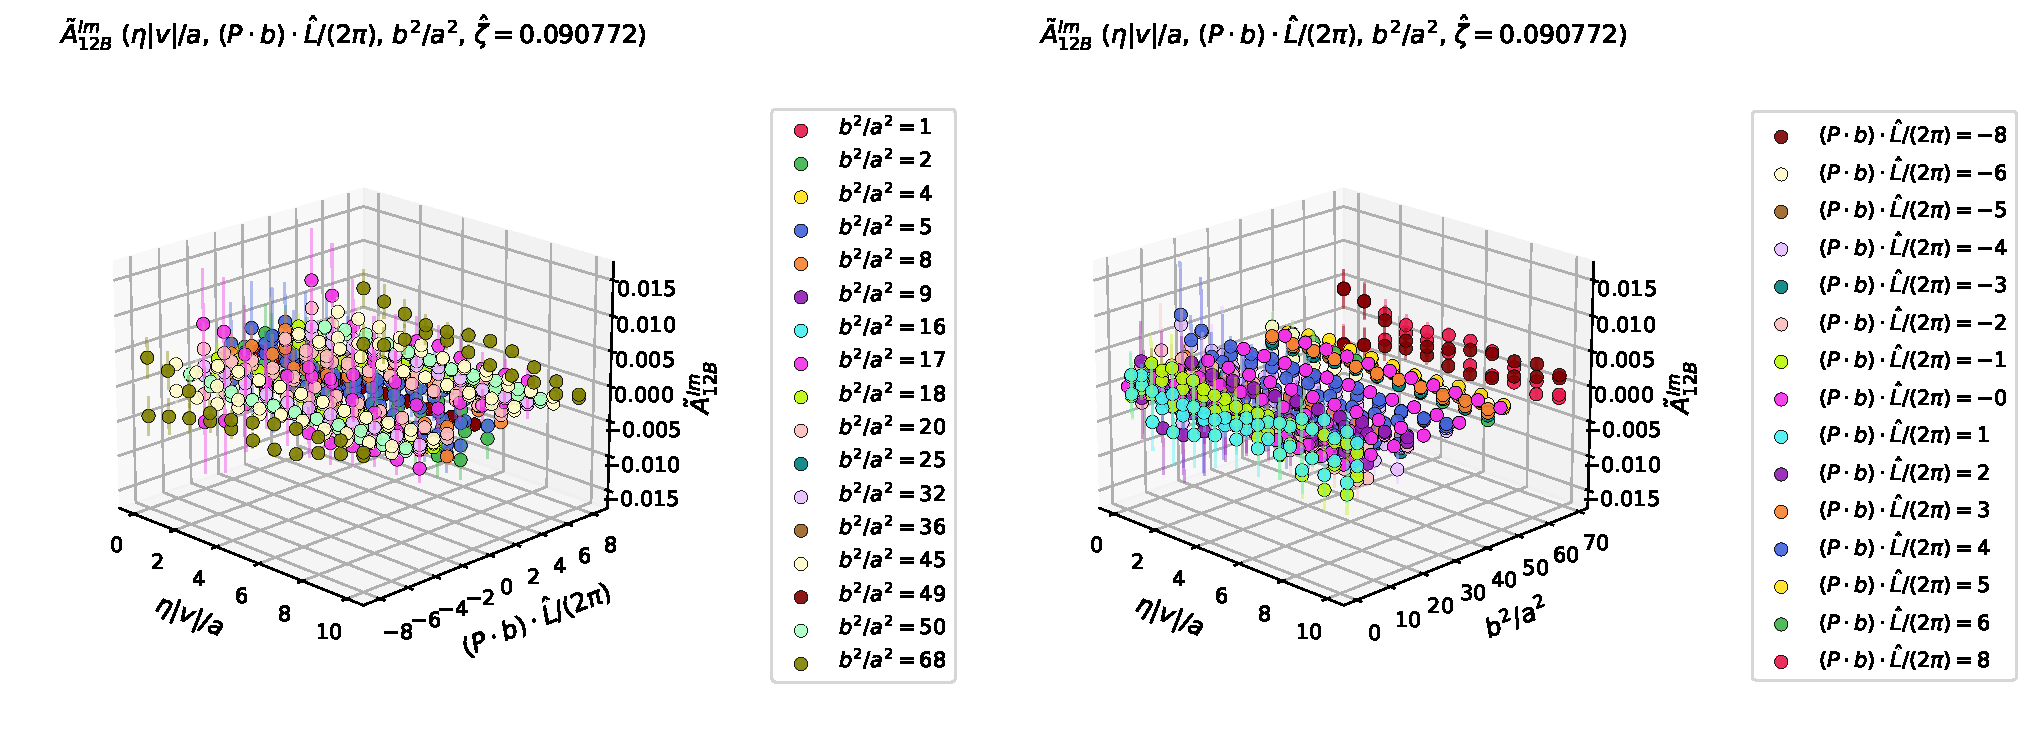
\includegraphics[width=0.98\linewidth,height=0.73\textheight,keepaspectratio]{ImA12B_Pb_bsq_PL-1_3D.pdf}\\[1mm]
{\small $\zetahat=0.090772$; $(\nu,s)$; staple-length dependence}
\figsrc{Thesis, Ch. 5: raw amplitude profiles; complete original panels.}
\end{frame}

\begin{frame}{$\tAmp_{2B}^{\mathrm{Re}}$ at $P_L=-1$: lattice coordinates}
\centering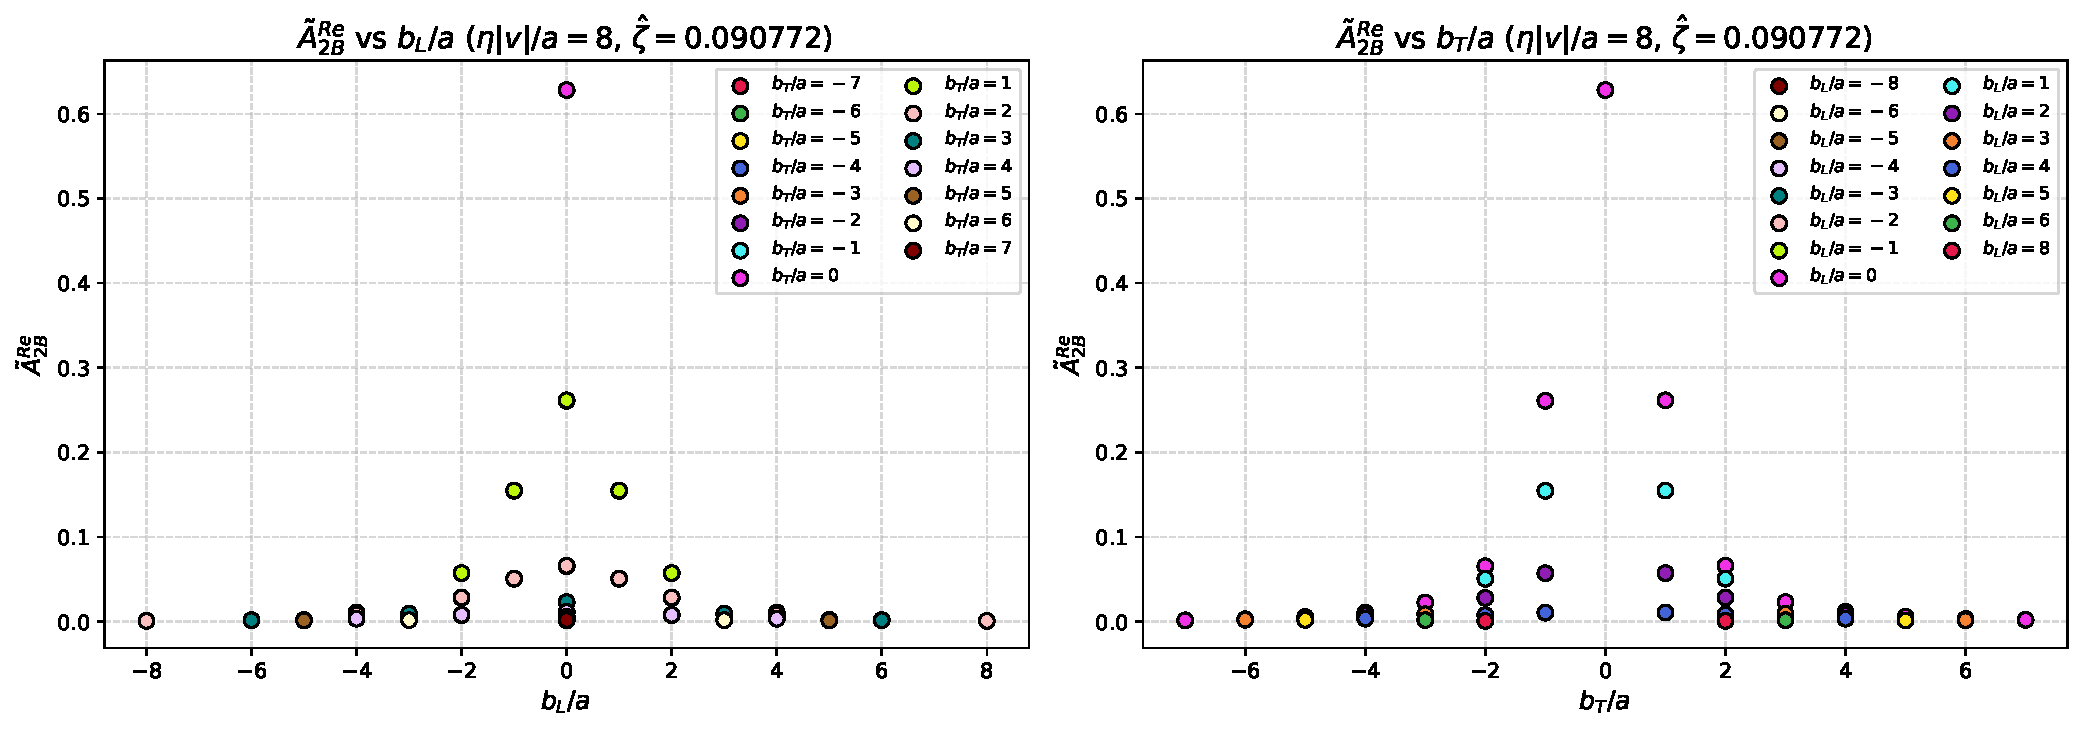
\includegraphics[width=0.98\linewidth,height=0.73\textheight,keepaspectratio]{ReA2B_eta8_PL-1_2D.pdf}\\[1mm]
{\small $\zetahat=0.090772$; $(b_L,b_T)$; $\eta|v|/a=8$ slices}
\figsrc{Thesis, Ch. 5: raw amplitude profiles; complete original panels.}
\end{frame}

\begin{frame}{$\tAmp_{2B}^{\mathrm{Re}}$ at $P_L=-1$: invariant coordinates}
\centering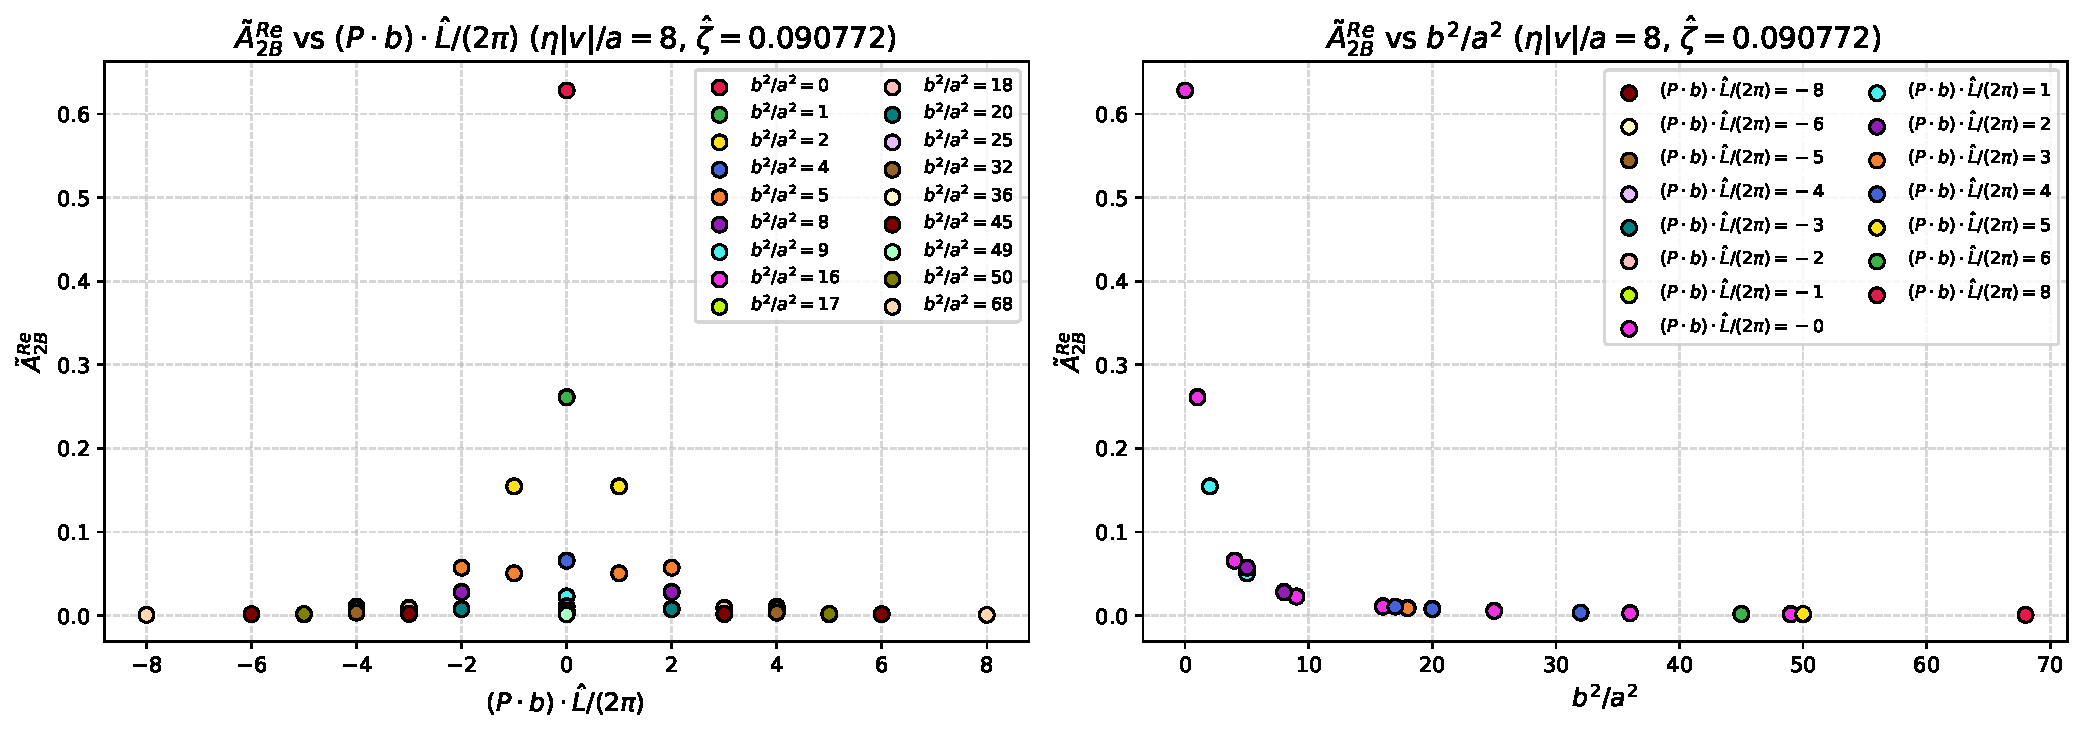
\includegraphics[width=0.98\linewidth,height=0.73\textheight,keepaspectratio]{ReA2B_Pb_bsq_eta8_PL-1_2D.pdf}\\[1mm]
{\small $\zetahat=0.090772$; $(\nu,s)$; $\eta|v|/a=8$ slices}
\figsrc{Thesis, Ch. 5: raw amplitude profiles; complete original panels.}
\end{frame}

\begin{frame}{$\tAmp_{2B}^{\mathrm{Im}}$ at $P_L=-1$: lattice coordinates}
\centering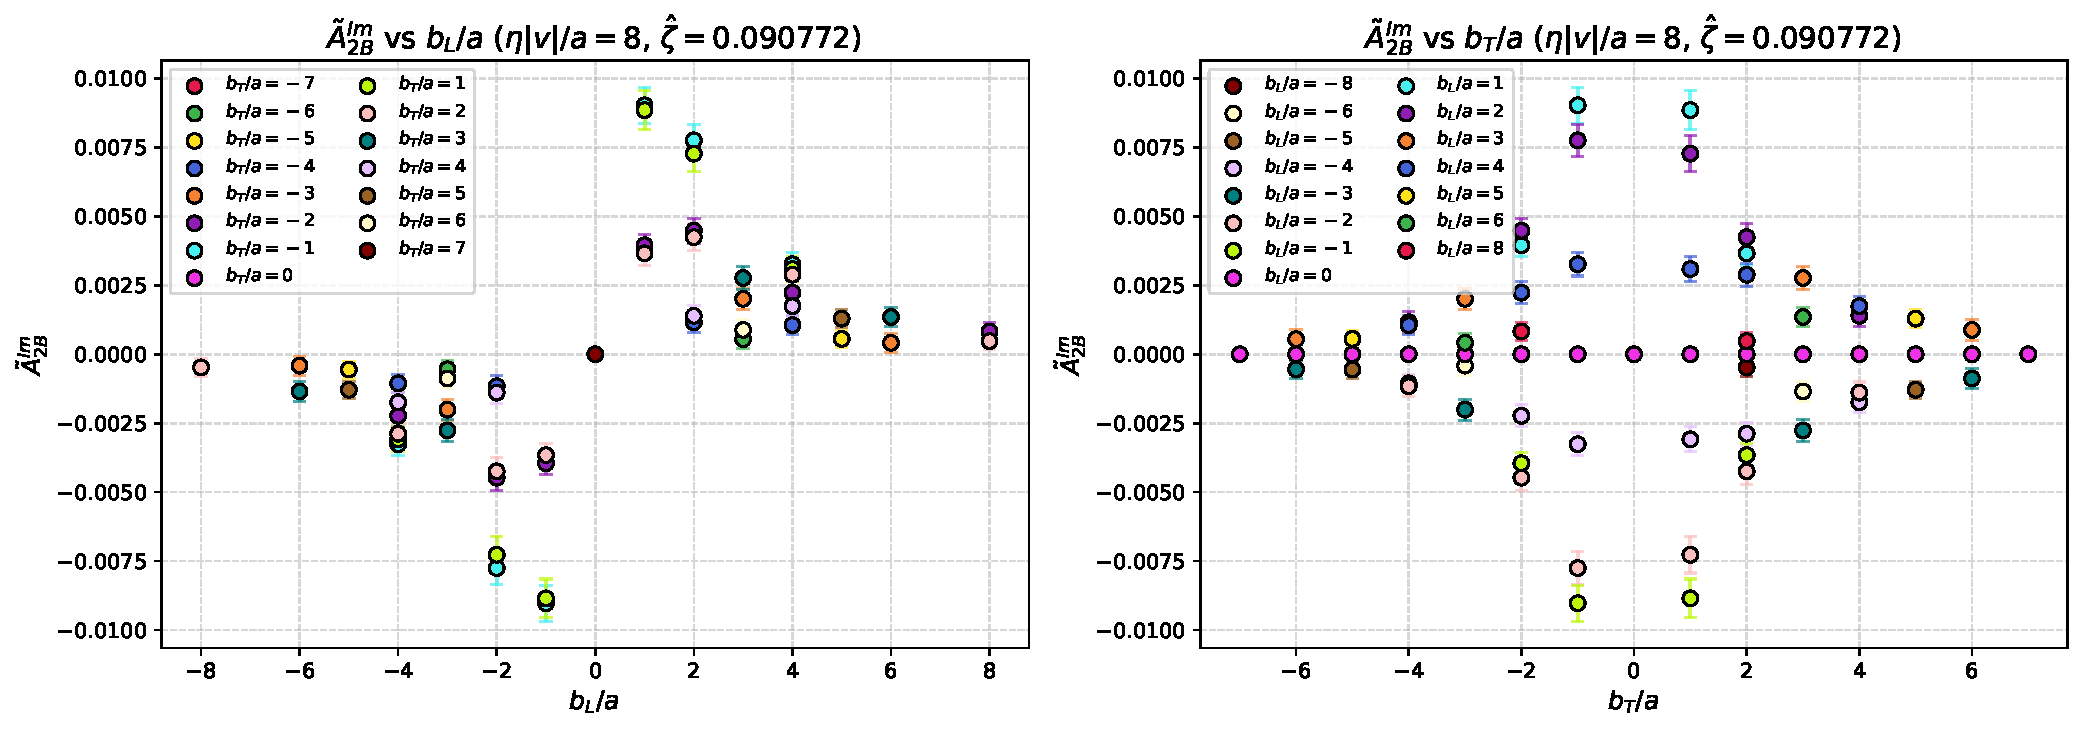
\includegraphics[width=0.98\linewidth,height=0.73\textheight,keepaspectratio]{ImA2B_eta8_PL-1_2D.pdf}\\[1mm]
{\small $\zetahat=0.090772$; $(b_L,b_T)$; $\eta|v|/a=8$ slices}
\figsrc{Thesis, Ch. 5: raw amplitude profiles; complete original panels.}
\end{frame}

\begin{frame}{$\tAmp_{2B}^{\mathrm{Im}}$ at $P_L=-1$: invariant coordinates}
\centering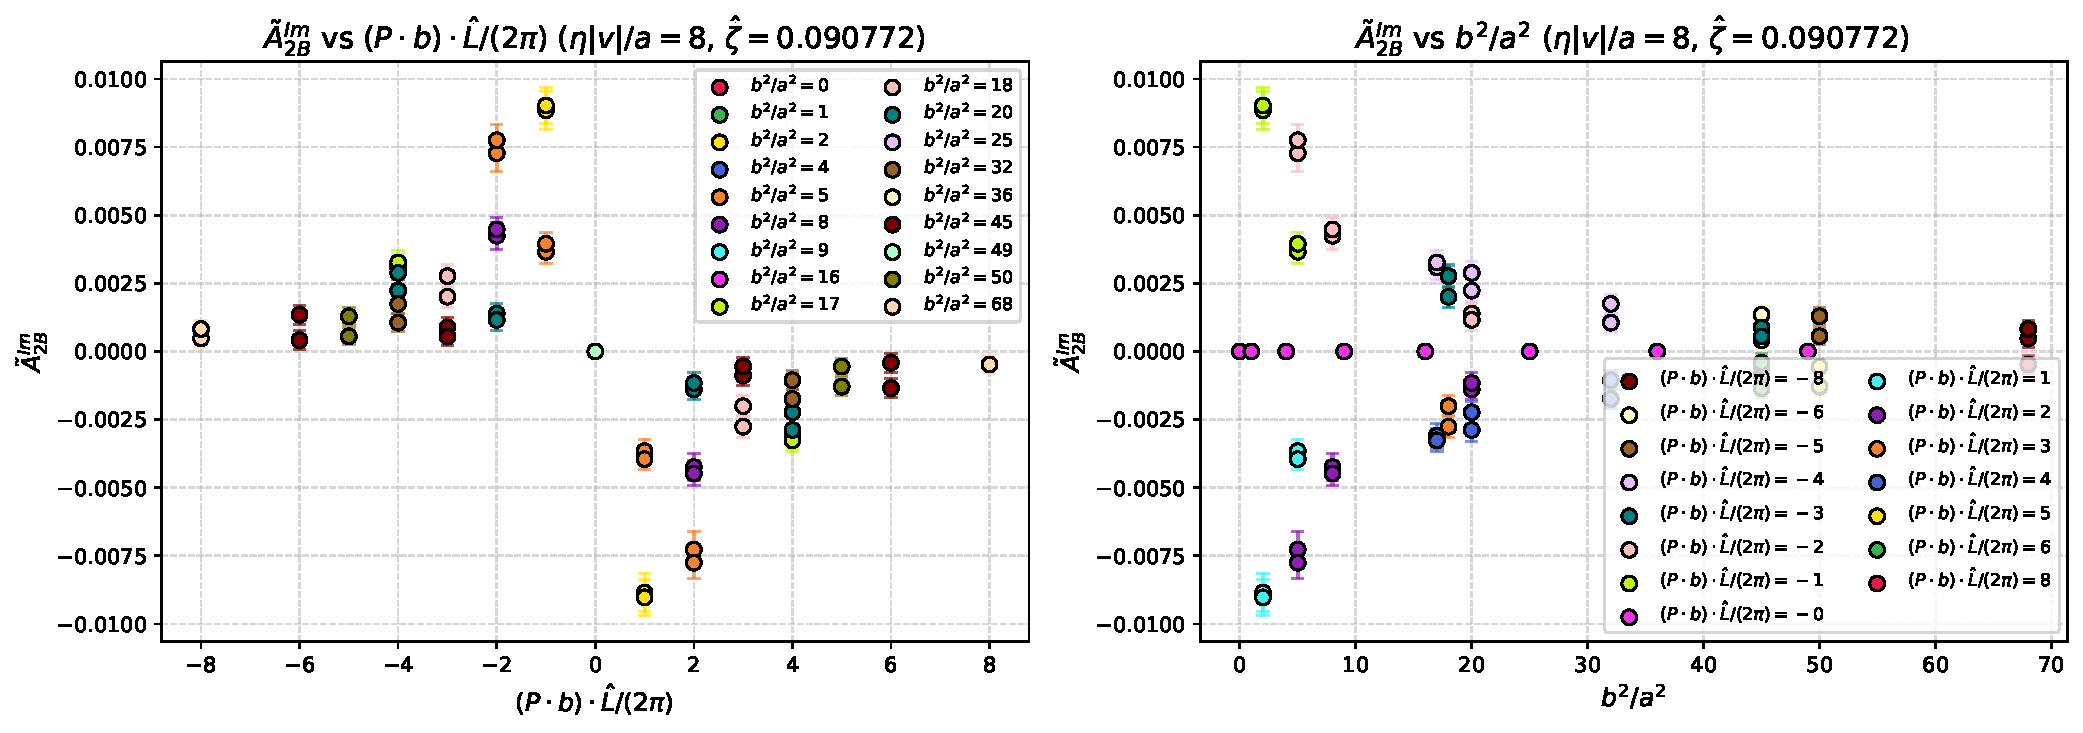
\includegraphics[width=0.98\linewidth,height=0.73\textheight,keepaspectratio]{ImA2B_Pb_bsq_eta8_PL-1_2D.pdf}\\[1mm]
{\small $\zetahat=0.090772$; $(\nu,s)$; $\eta|v|/a=8$ slices}
\figsrc{Thesis, Ch. 5: raw amplitude profiles; complete original panels.}
\end{frame}

\begin{frame}{$\tAmp_{12B}^{\mathrm{Re}}$ at $P_L=-1$: lattice coordinates}
\centering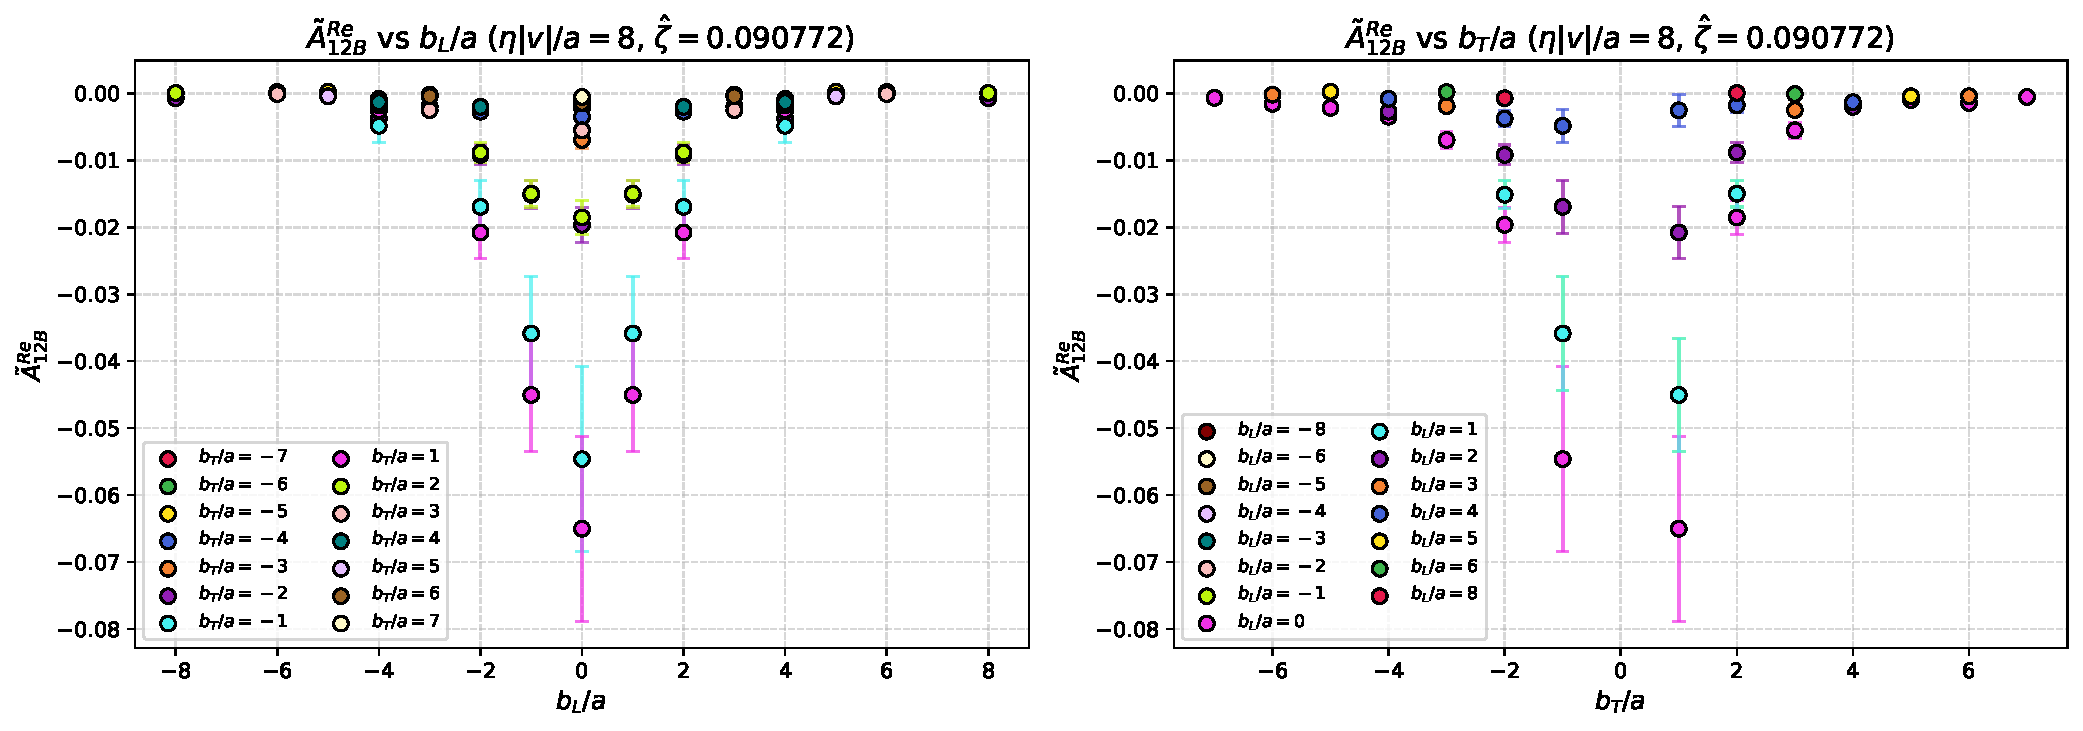
\includegraphics[width=0.98\linewidth,height=0.73\textheight,keepaspectratio]{ReA12B_eta8_PL-1_2D.pdf}\\[1mm]
{\small $\zetahat=0.090772$; $(b_L,b_T)$; $\eta|v|/a=8$ slices}
\figsrc{Thesis, Ch. 5: raw amplitude profiles; complete original panels.}
\end{frame}

\begin{frame}{$\tAmp_{12B}^{\mathrm{Re}}$ at $P_L=-1$: invariant coordinates}
\centering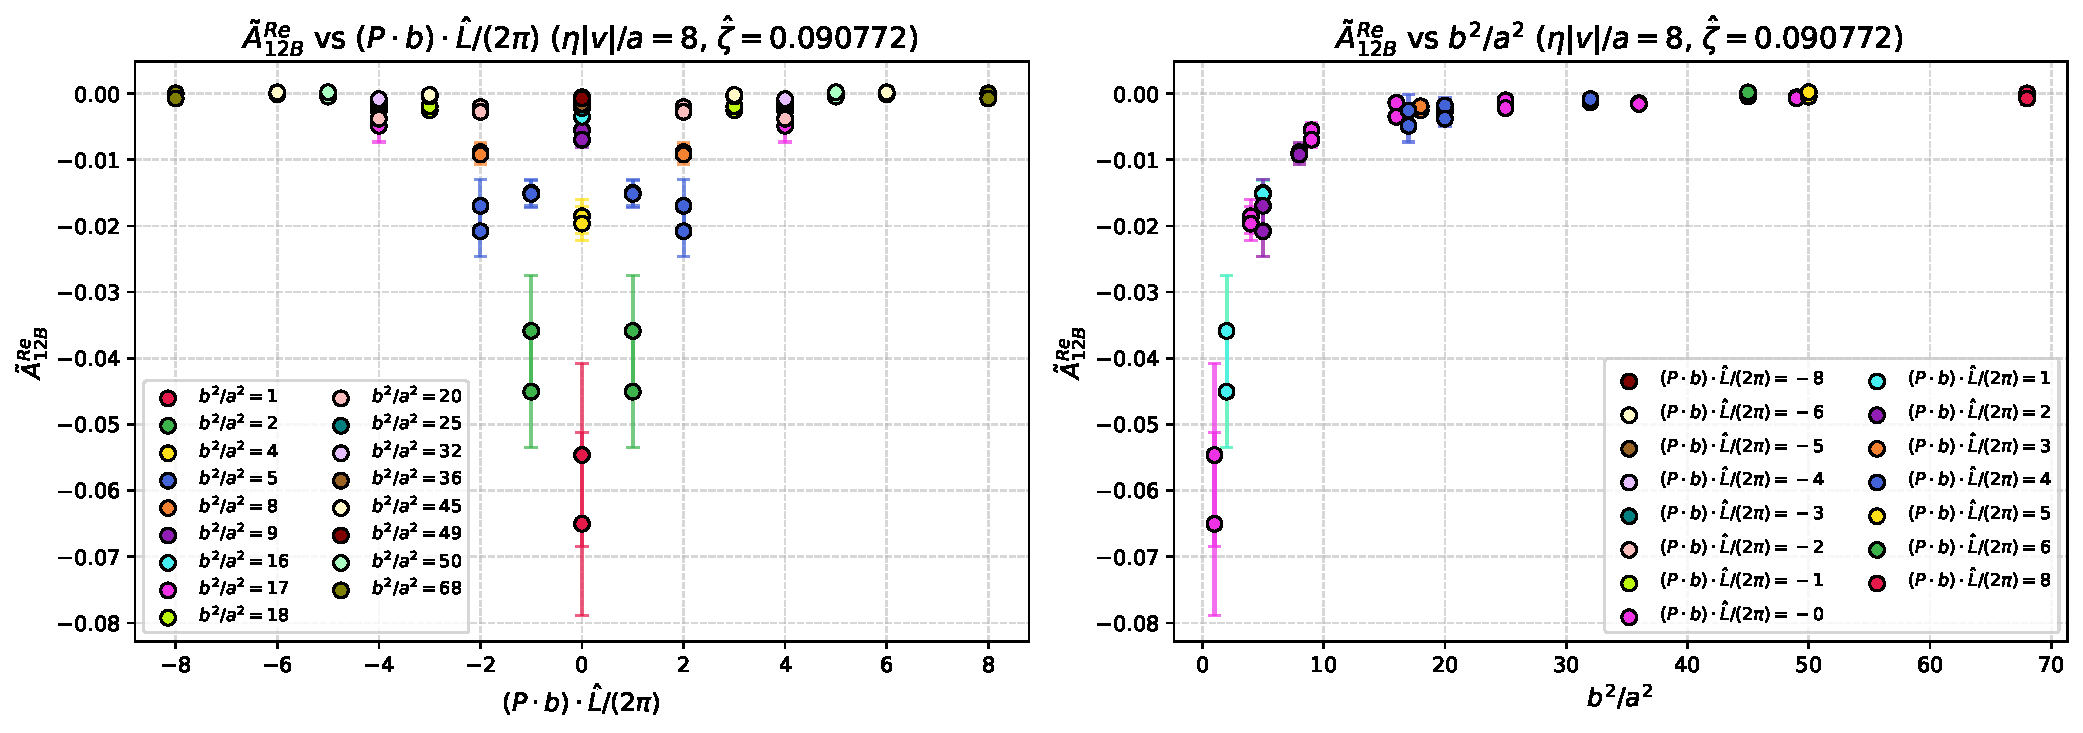
\includegraphics[width=0.98\linewidth,height=0.73\textheight,keepaspectratio]{ReA12B_Pb_bsq_eta8_PL-1_2D.pdf}\\[1mm]
{\small $\zetahat=0.090772$; $(\nu,s)$; $\eta|v|/a=8$ slices}
\figsrc{Thesis, Ch. 5: raw amplitude profiles; complete original panels.}
\end{frame}

\begin{frame}{$\tAmp_{12B}^{\mathrm{Im}}$ at $P_L=-1$: lattice coordinates}
\centering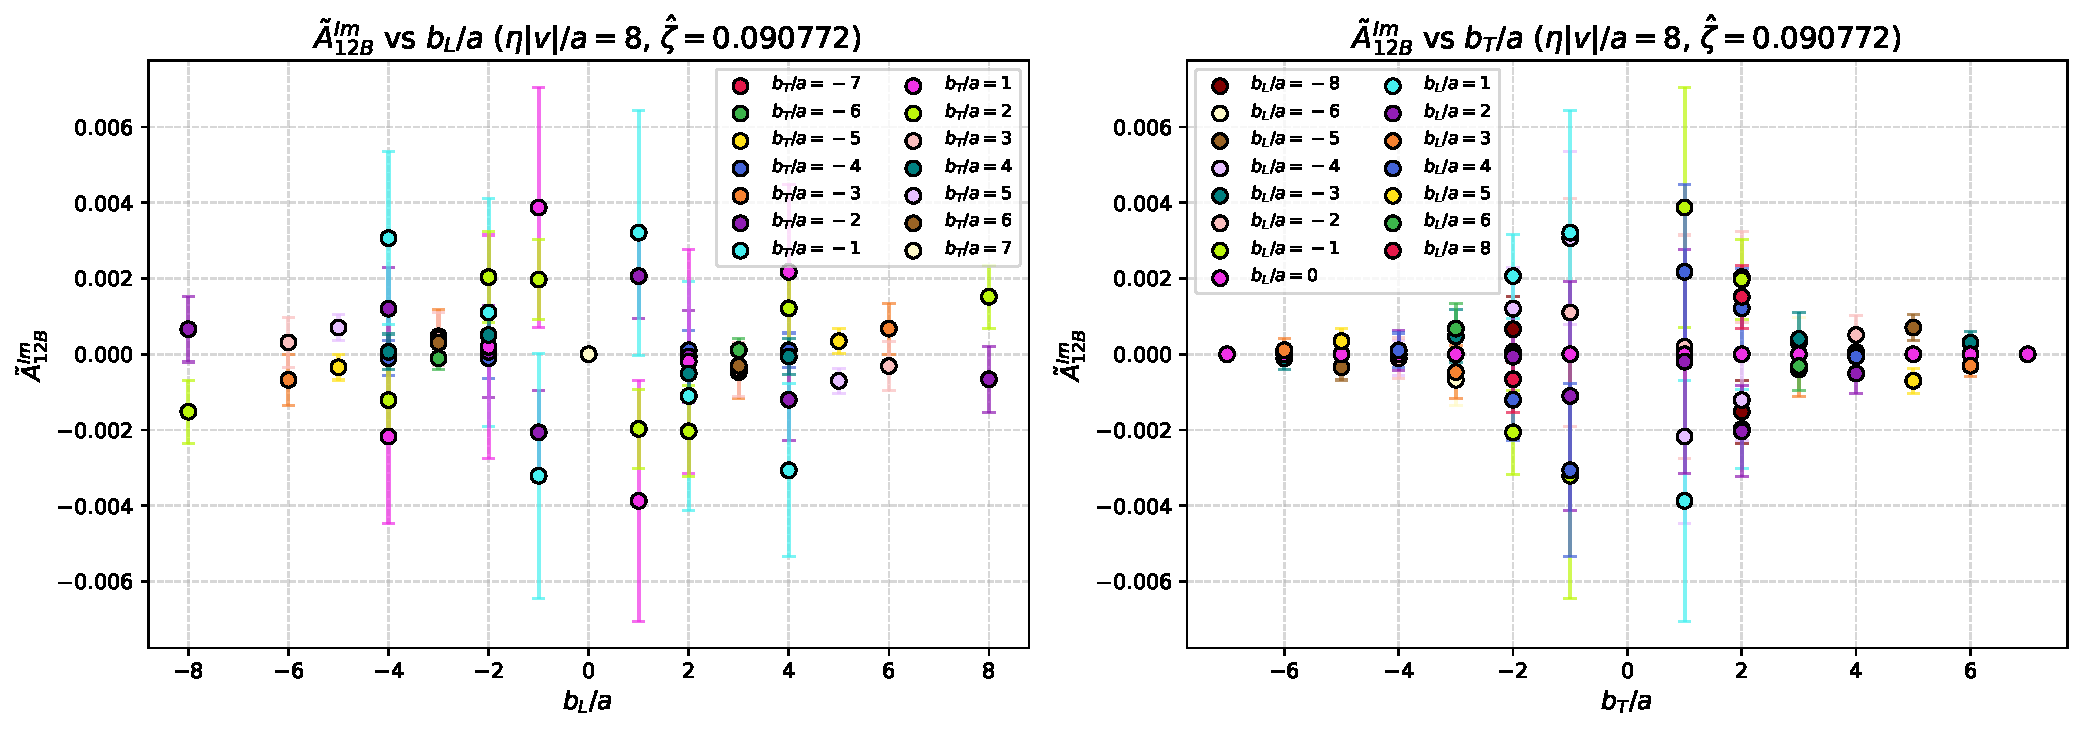
\includegraphics[width=0.98\linewidth,height=0.73\textheight,keepaspectratio]{ImA12B_eta8_PL-1_2D.pdf}\\[1mm]
{\small $\zetahat=0.090772$; $(b_L,b_T)$; $\eta|v|/a=8$ slices}
\figsrc{Thesis, Ch. 5: raw amplitude profiles; complete original panels.}
\end{frame}

\begin{frame}{$\tAmp_{12B}^{\mathrm{Im}}$ at $P_L=-1$: invariant coordinates}
\centering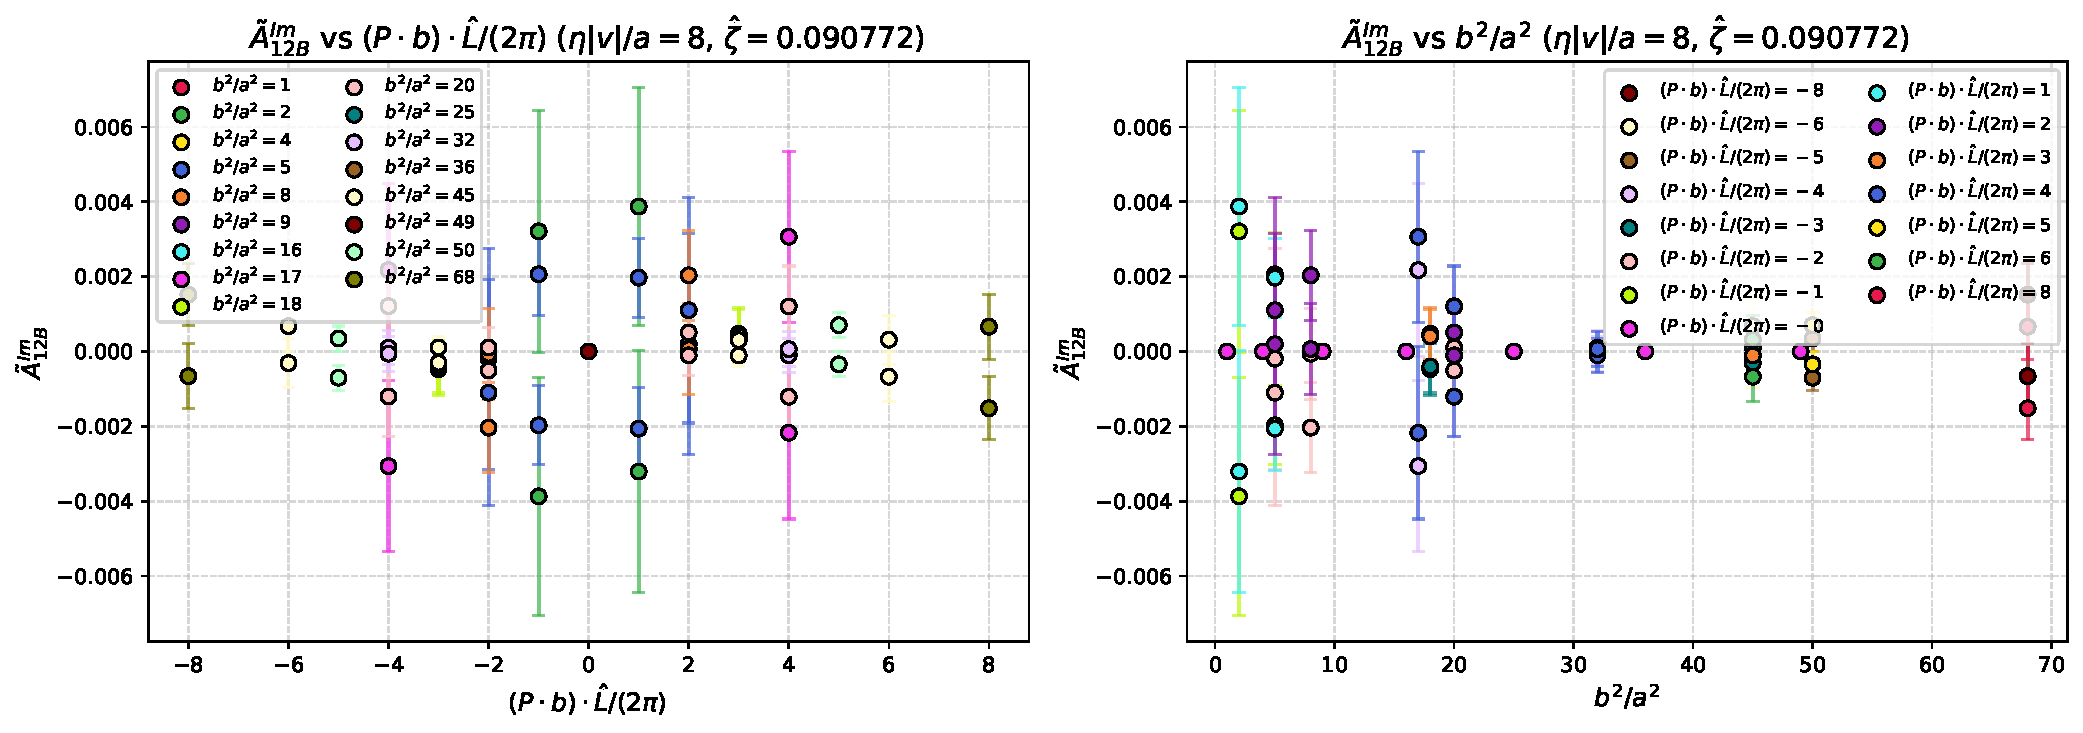
\includegraphics[width=0.98\linewidth,height=0.73\textheight,keepaspectratio]{ImA12B_Pb_bsq_eta8_PL-1_2D.pdf}\\[1mm]
{\small $\zetahat=0.090772$; $(\nu,s)$; $\eta|v|/a=8$ slices}
\figsrc{Thesis, Ch. 5: raw amplitude profiles; complete original panels.}
\end{frame}

\begin{frame}{$\tAmp_{2B}^{\mathrm{Re}}$ at $P_L=-2$: lattice coordinates}
\centering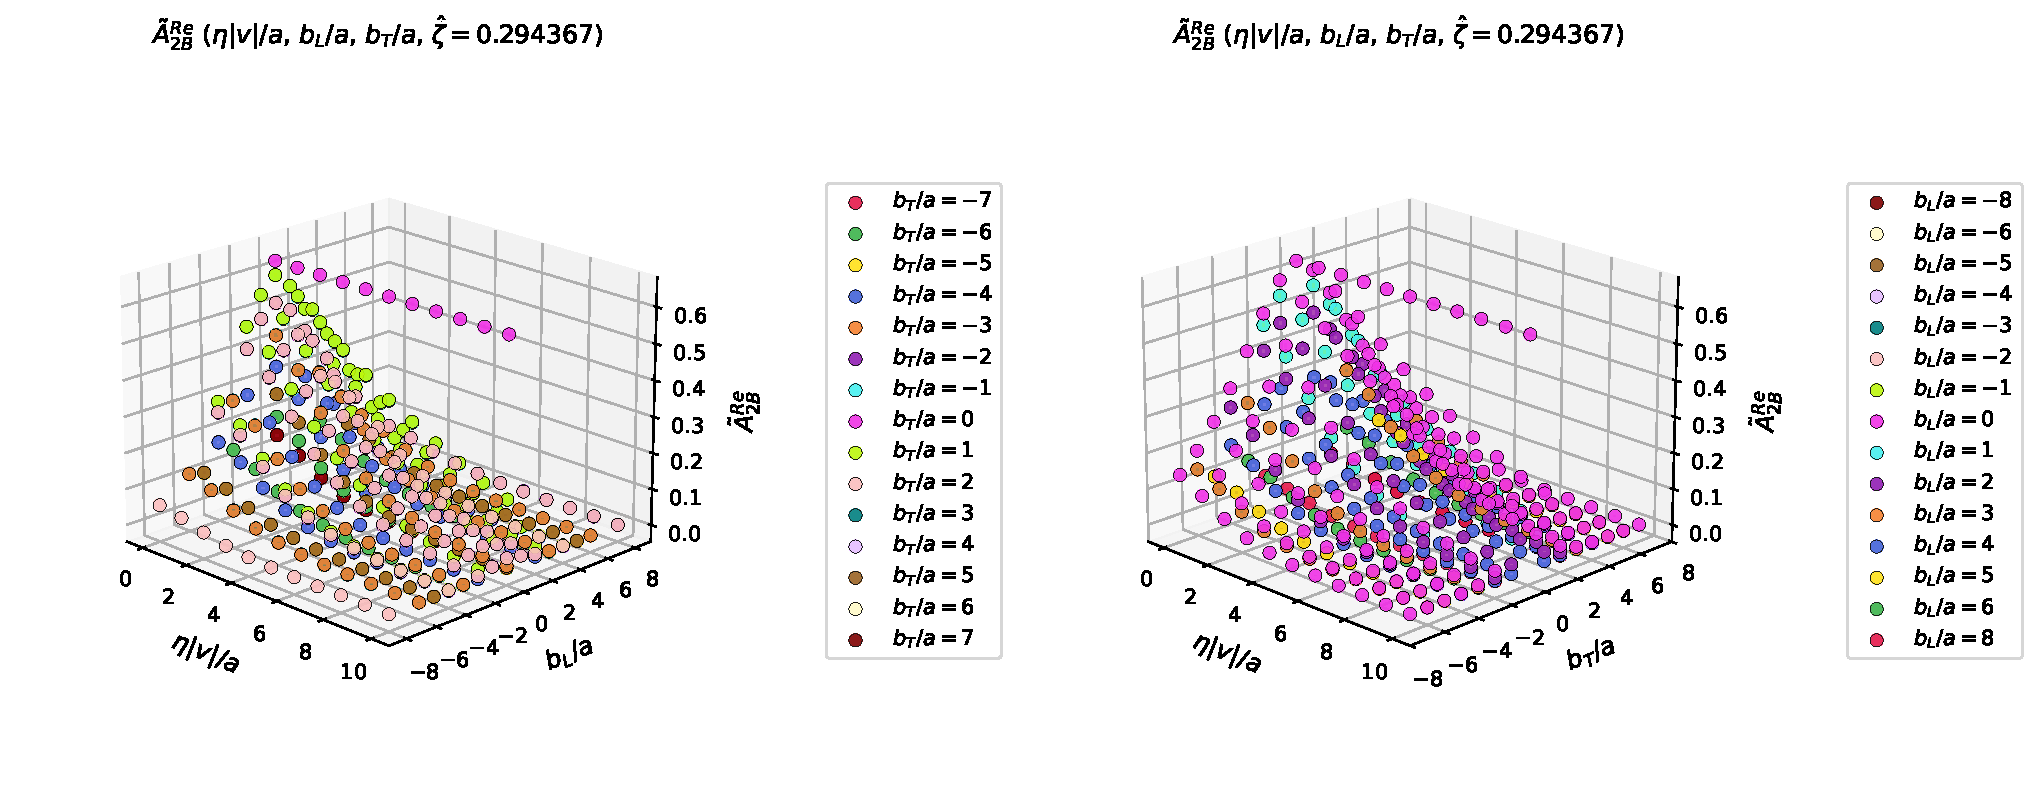
\includegraphics[width=0.98\linewidth,height=0.73\textheight,keepaspectratio]{ReA2B_PL-2_3D.pdf}\\[1mm]
{\small $\zetahat=0.294367$; $(b_L,b_T)$; staple-length dependence}
\figsrc{Thesis, Ch. 5: raw amplitude profiles; complete original panels.}
\end{frame}

\begin{frame}{$\tAmp_{2B}^{\mathrm{Re}}$ at $P_L=-2$: invariant coordinates}
\centering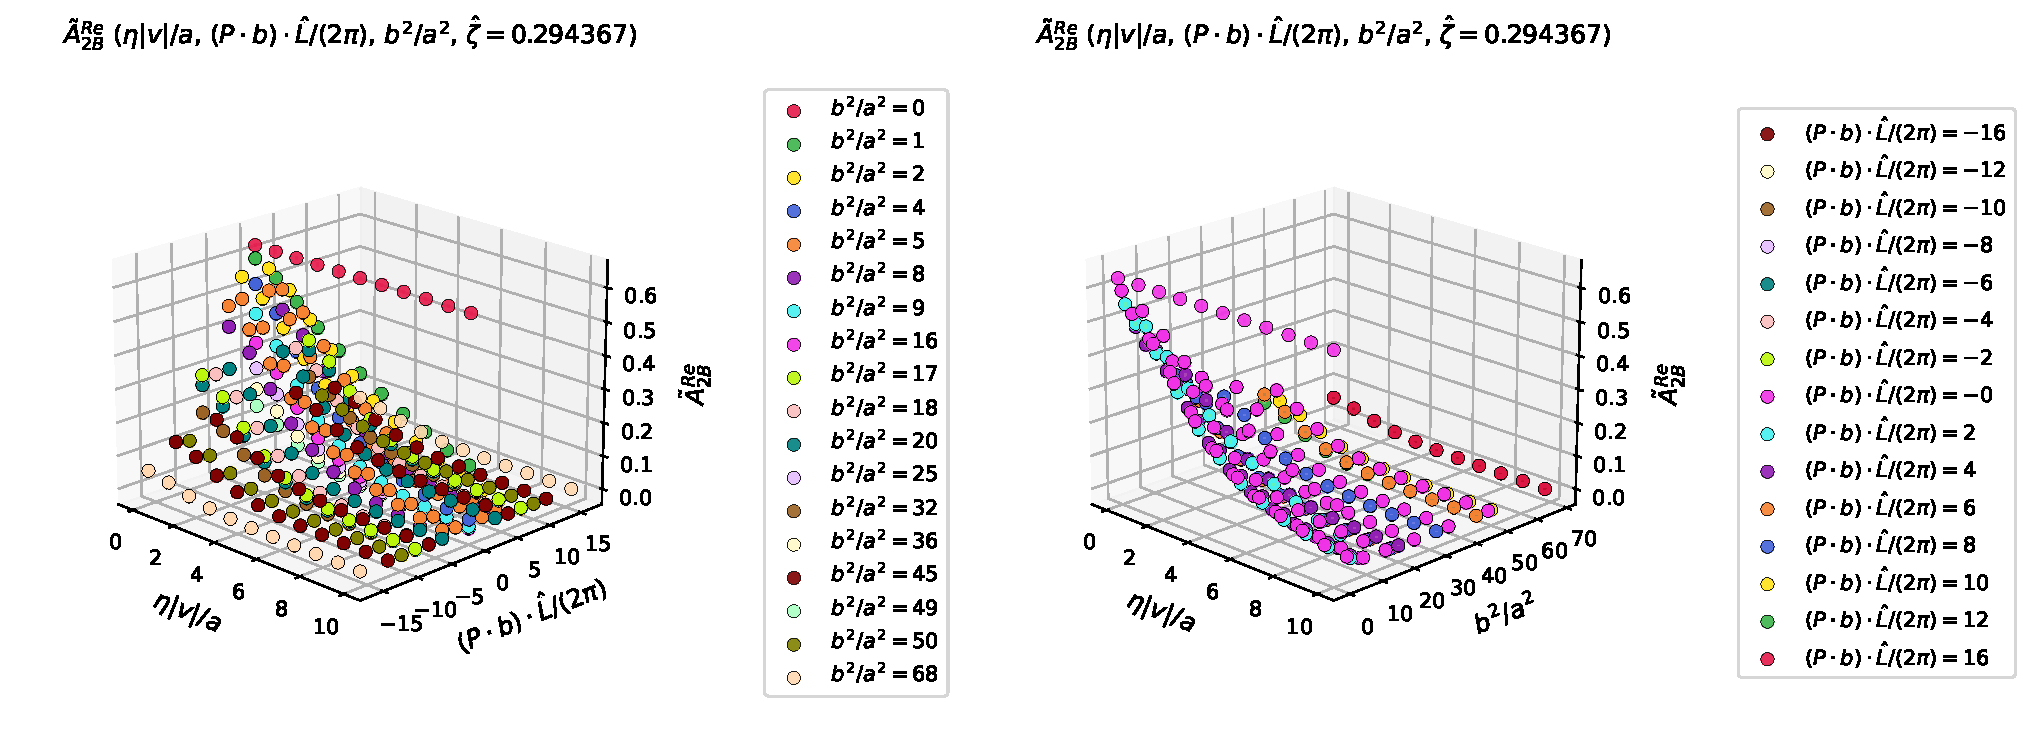
\includegraphics[width=0.98\linewidth,height=0.73\textheight,keepaspectratio]{ReA2B_Pb_bsq_PL-2_3D.pdf}\\[1mm]
{\small $\zetahat=0.294367$; $(\nu,s)$; staple-length dependence}
\figsrc{Thesis, Ch. 5: raw amplitude profiles; complete original panels.}
\end{frame}

\begin{frame}{$\tAmp_{2B}^{\mathrm{Im}}$ at $P_L=-2$: lattice coordinates}
\centering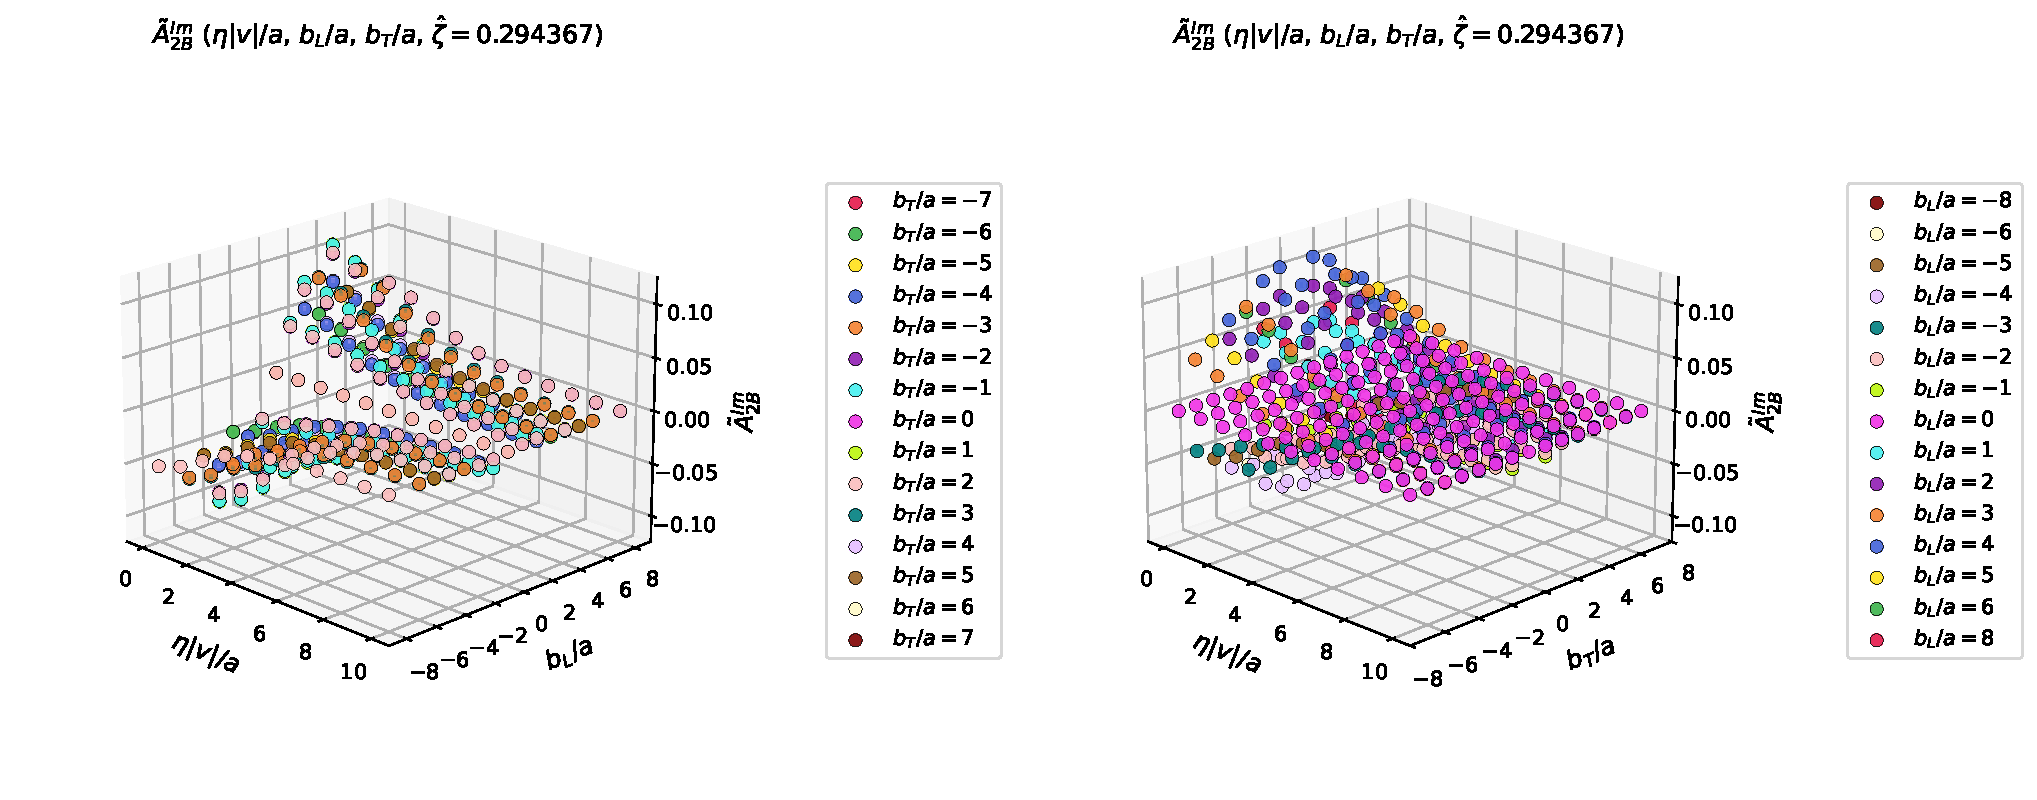
\includegraphics[width=0.98\linewidth,height=0.73\textheight,keepaspectratio]{ImA2B_PL-2_3D.pdf}\\[1mm]
{\small $\zetahat=0.294367$; $(b_L,b_T)$; staple-length dependence}
\figsrc{Thesis, Ch. 5: raw amplitude profiles; complete original panels.}
\end{frame}

\begin{frame}{$\tAmp_{2B}^{\mathrm{Im}}$ at $P_L=-2$: invariant coordinates}
\centering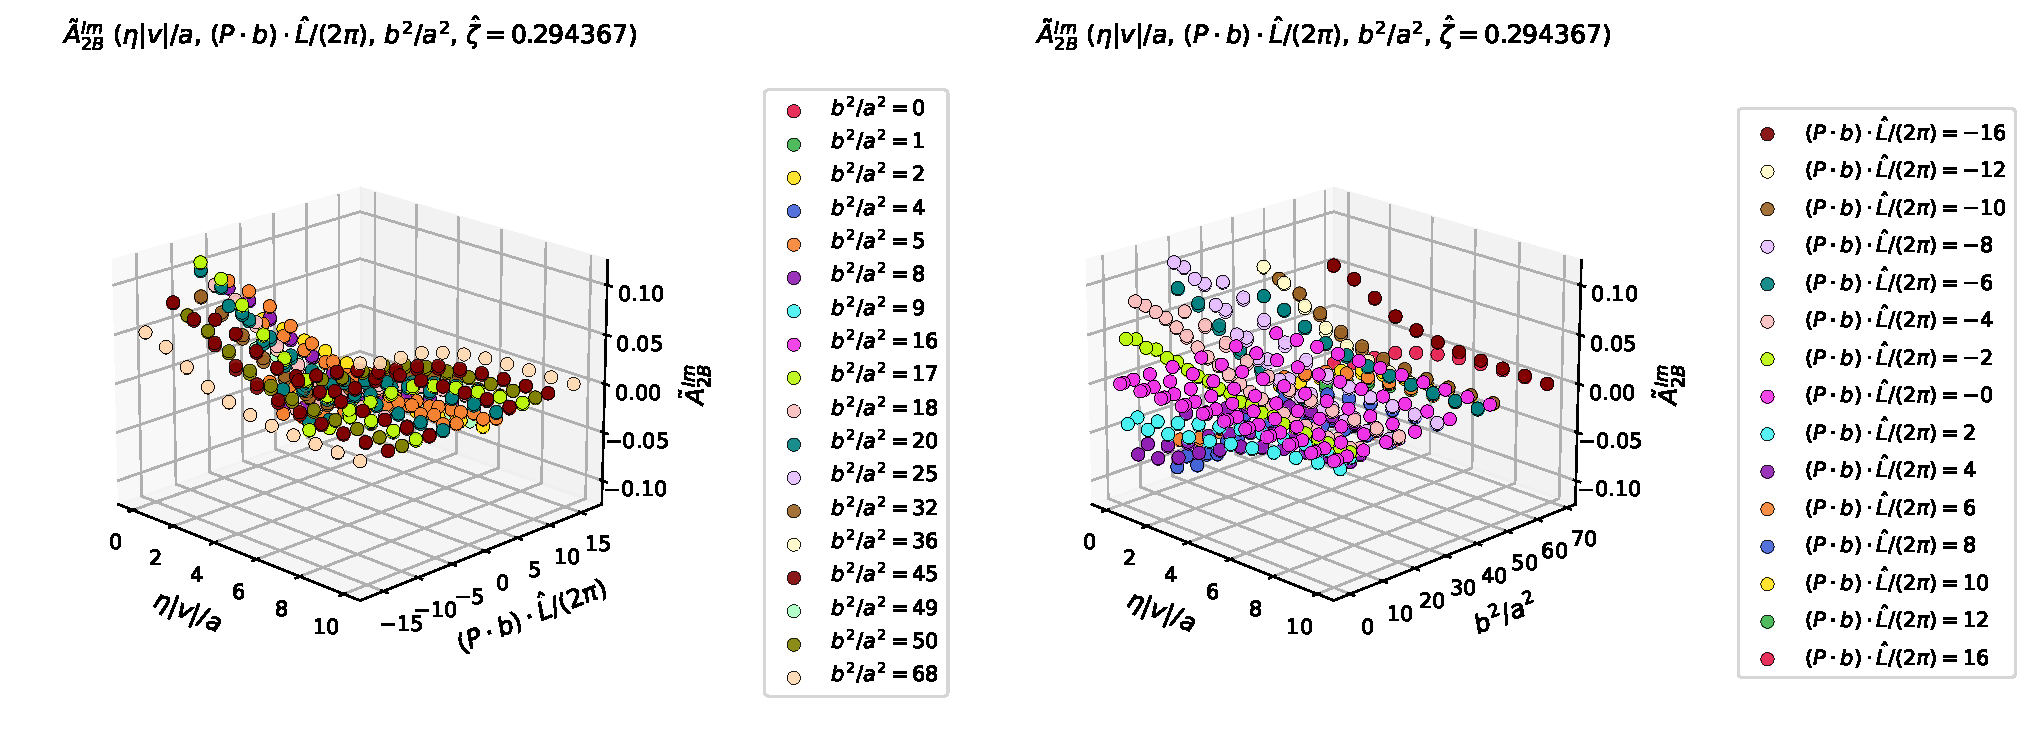
\includegraphics[width=0.98\linewidth,height=0.73\textheight,keepaspectratio]{ImA2B_Pb_bsq_PL-2_3D.pdf}\\[1mm]
{\small $\zetahat=0.294367$; $(\nu,s)$; staple-length dependence}
\figsrc{Thesis, Ch. 5: raw amplitude profiles; complete original panels.}
\end{frame}

\begin{frame}{$\tAmp_{12B}^{\mathrm{Re}}$ at $P_L=-2$: lattice coordinates}
\centering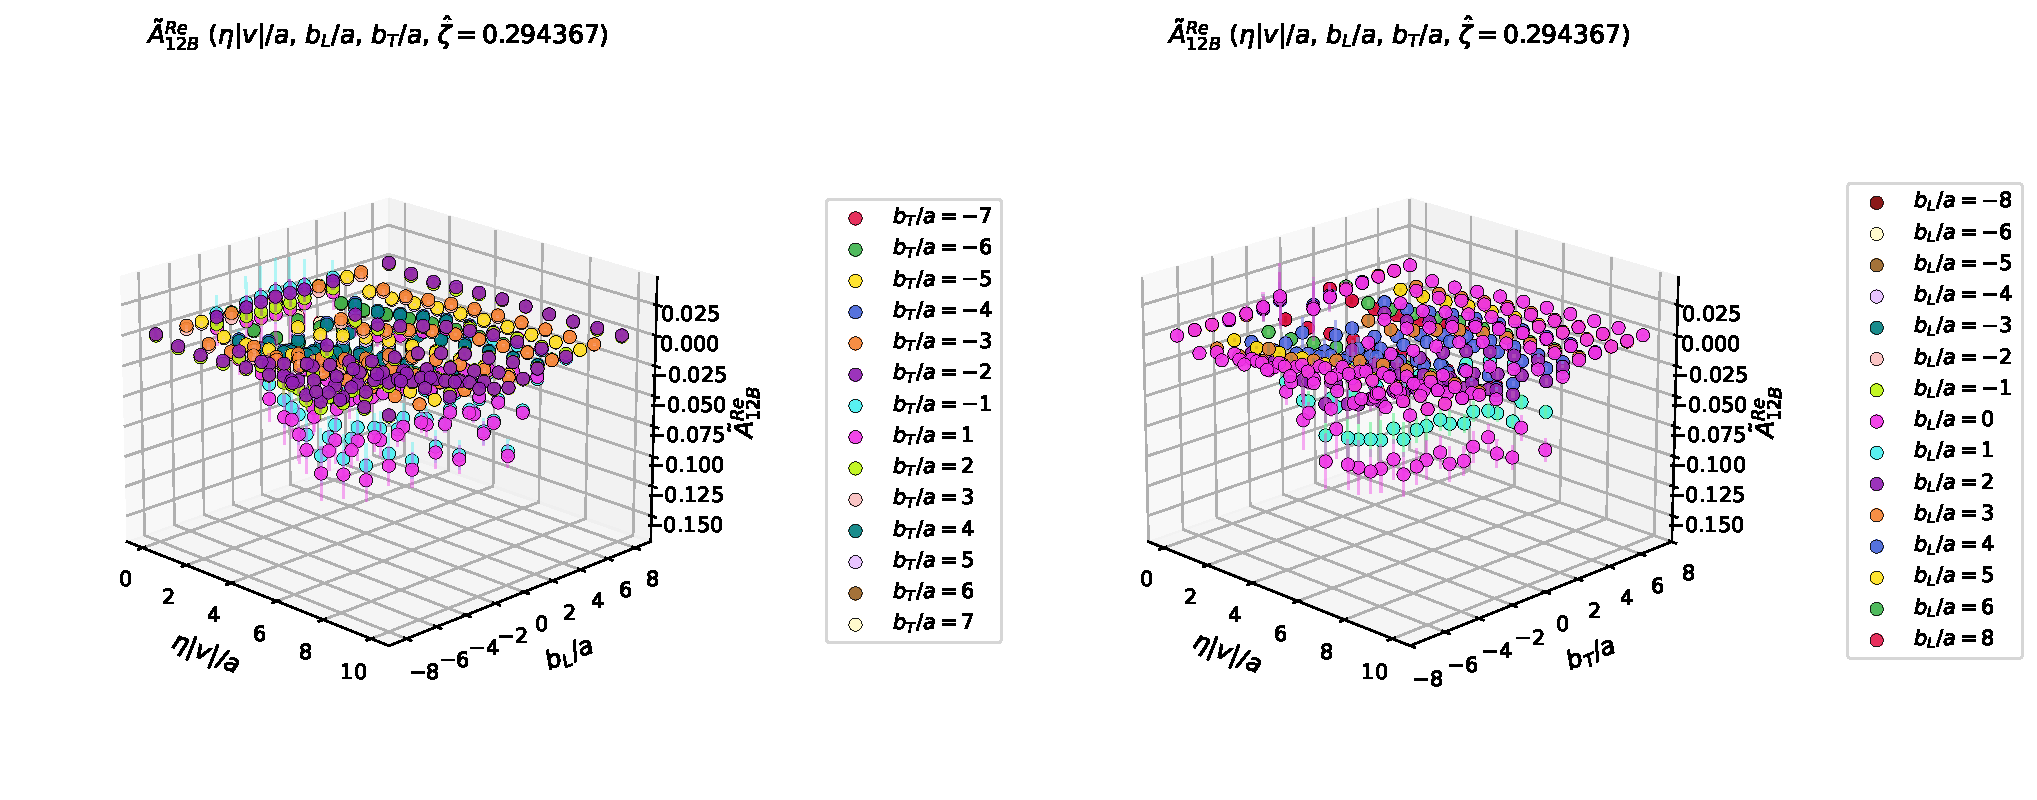
\includegraphics[width=0.98\linewidth,height=0.73\textheight,keepaspectratio]{ReA12B_PL-2_3D.pdf}\\[1mm]
{\small $\zetahat=0.294367$; $(b_L,b_T)$; staple-length dependence}
\figsrc{Thesis, Ch. 5: raw amplitude profiles; complete original panels.}
\end{frame}

\begin{frame}{$\tAmp_{12B}^{\mathrm{Re}}$ at $P_L=-2$: invariant coordinates}
\centering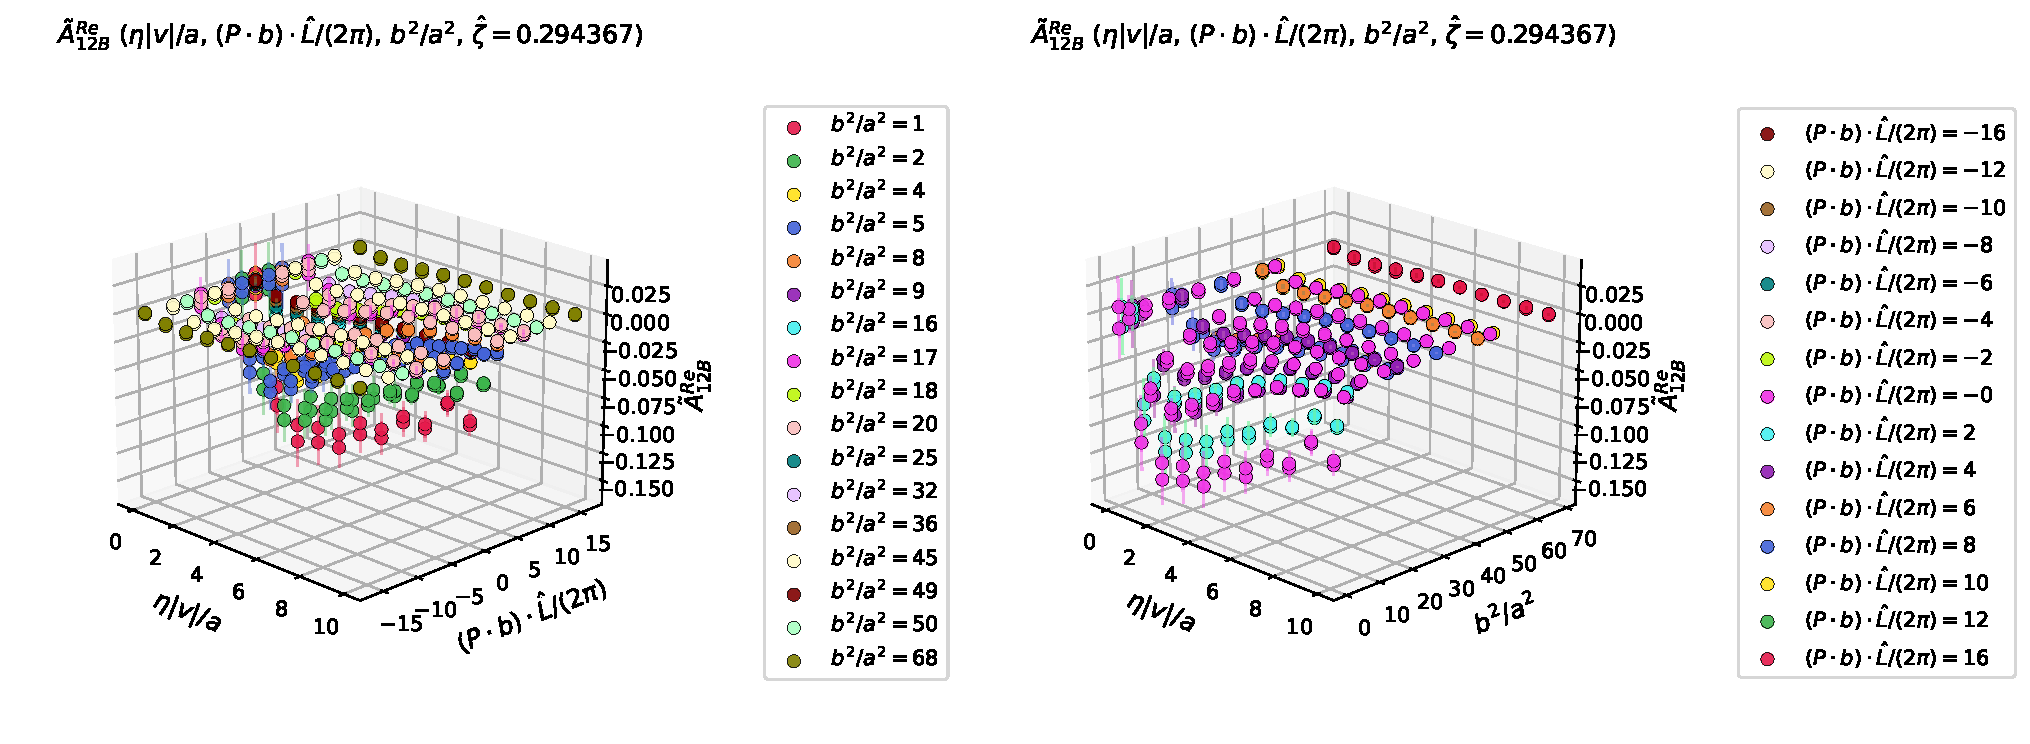
\includegraphics[width=0.98\linewidth,height=0.73\textheight,keepaspectratio]{ReA12B_Pb_bsq_PL-2_3D.pdf}\\[1mm]
{\small $\zetahat=0.294367$; $(\nu,s)$; staple-length dependence}
\figsrc{Thesis, Ch. 5: raw amplitude profiles; complete original panels.}
\end{frame}

\begin{frame}{$\tAmp_{12B}^{\mathrm{Im}}$ at $P_L=-2$: lattice coordinates}
\centering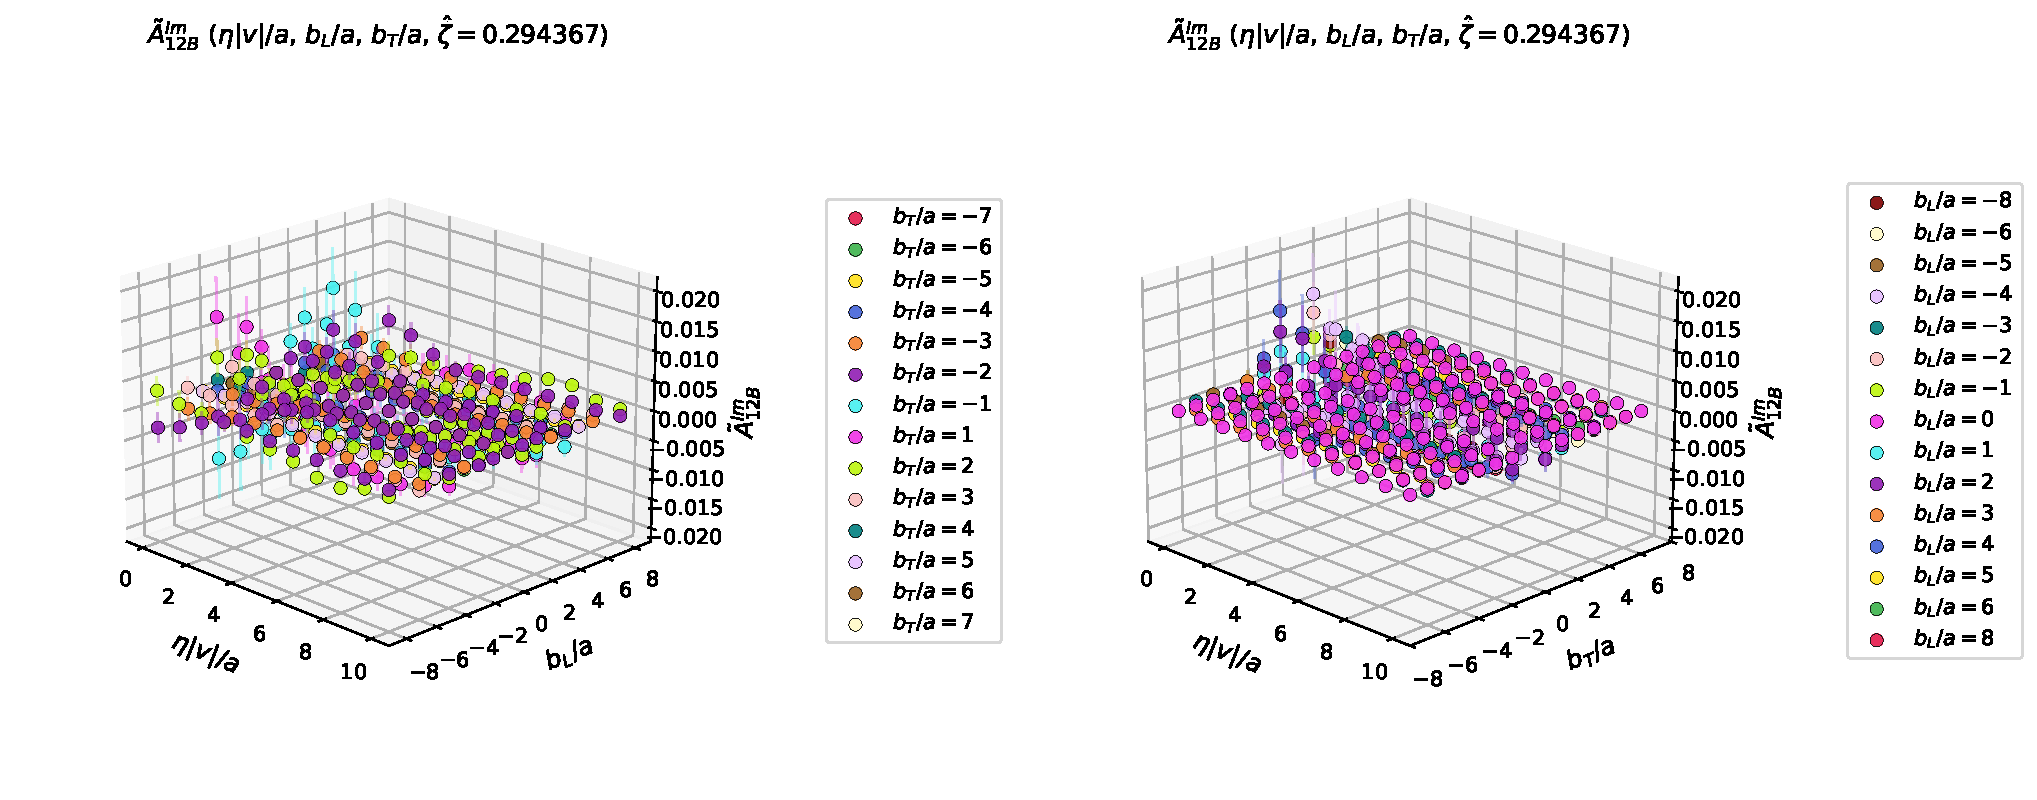
\includegraphics[width=0.98\linewidth,height=0.73\textheight,keepaspectratio]{ImA12B_PL-2_3D.pdf}\\[1mm]
{\small $\zetahat=0.294367$; $(b_L,b_T)$; staple-length dependence}
\figsrc{Thesis, Ch. 5: raw amplitude profiles; complete original panels.}
\end{frame}

\begin{frame}{$\tAmp_{12B}^{\mathrm{Im}}$ at $P_L=-2$: invariant coordinates}
\centering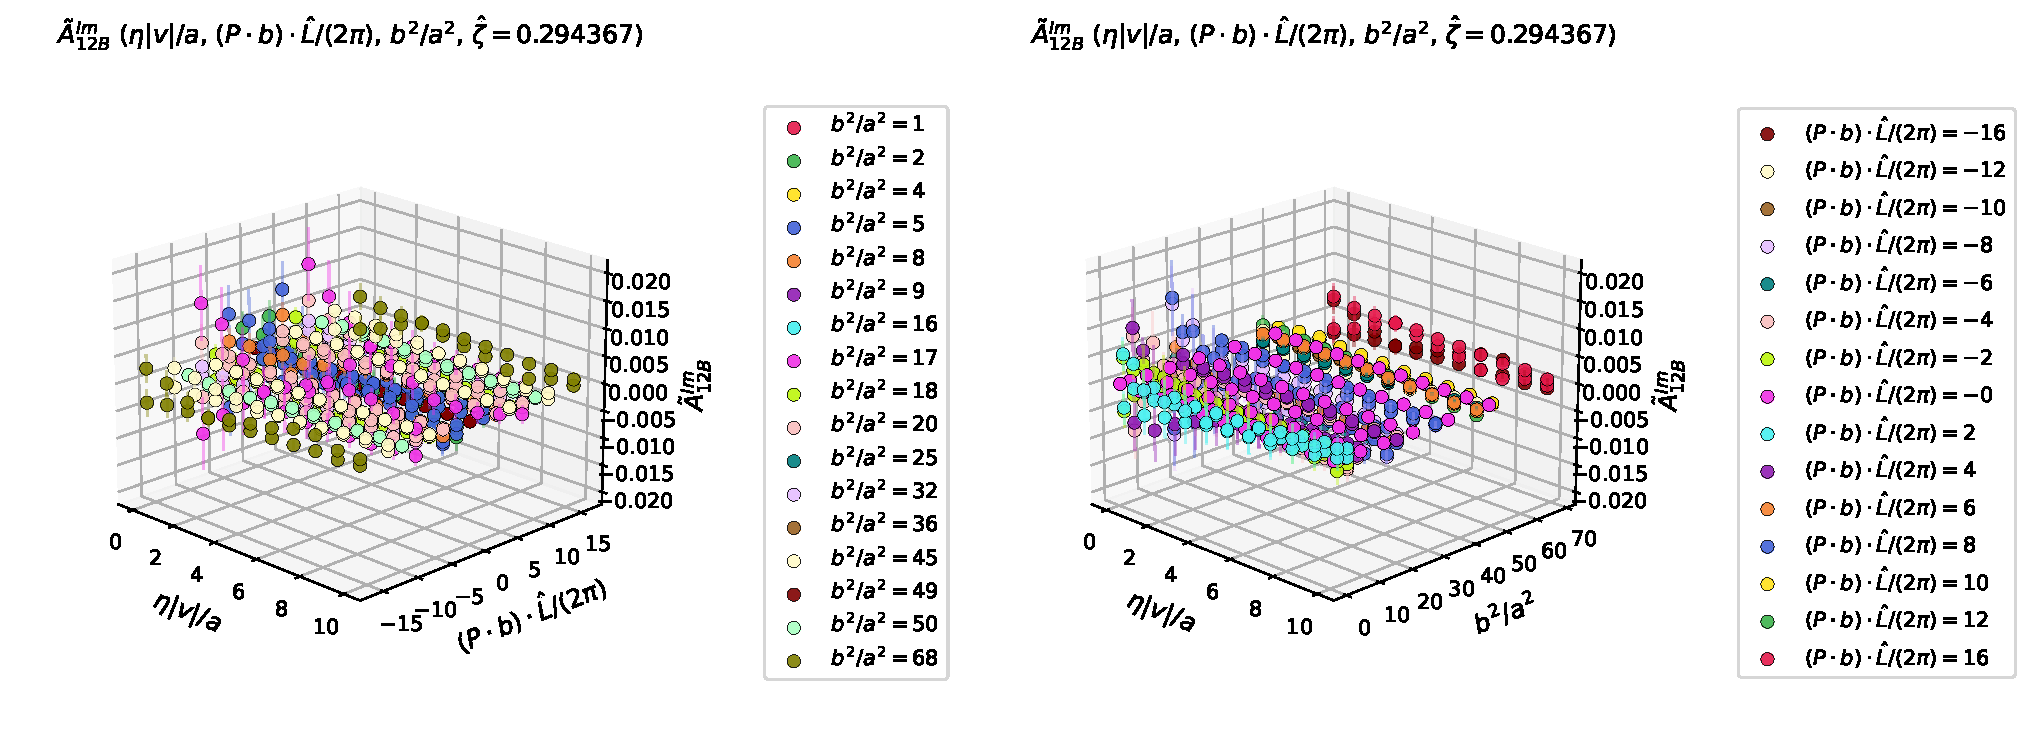
\includegraphics[width=0.98\linewidth,height=0.73\textheight,keepaspectratio]{ImA12B_Pb_bsq_PL-2_3D.pdf}\\[1mm]
{\small $\zetahat=0.294367$; $(\nu,s)$; staple-length dependence}
\figsrc{Thesis, Ch. 5: raw amplitude profiles; complete original panels.}
\end{frame}

\begin{frame}{$\tAmp_{2B}^{\mathrm{Re}}$ at $P_L=-2$: lattice coordinates}
\centering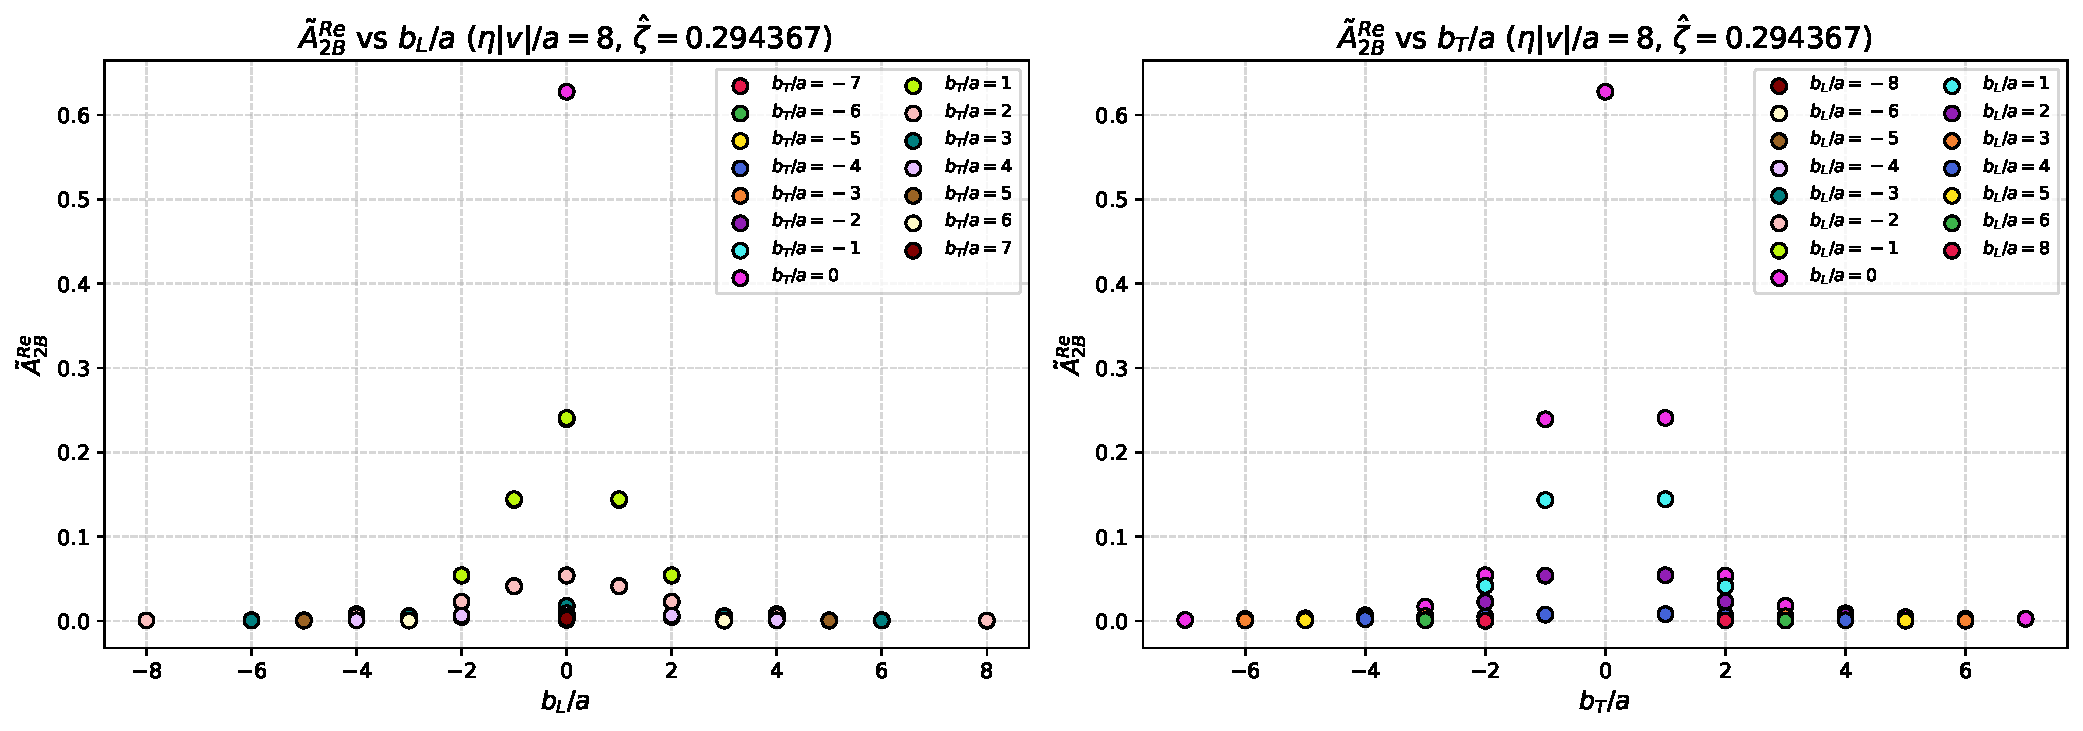
\includegraphics[width=0.98\linewidth,height=0.73\textheight,keepaspectratio]{ReA2B_eta8_PL-2_2D.pdf}\\[1mm]
{\small $\zetahat=0.294367$; $(b_L,b_T)$; $\eta|v|/a=8$ slices}
\figsrc{Thesis, Ch. 5: raw amplitude profiles; complete original panels.}
\end{frame}

\begin{frame}{$\tAmp_{2B}^{\mathrm{Re}}$ at $P_L=-2$: invariant coordinates}
\centering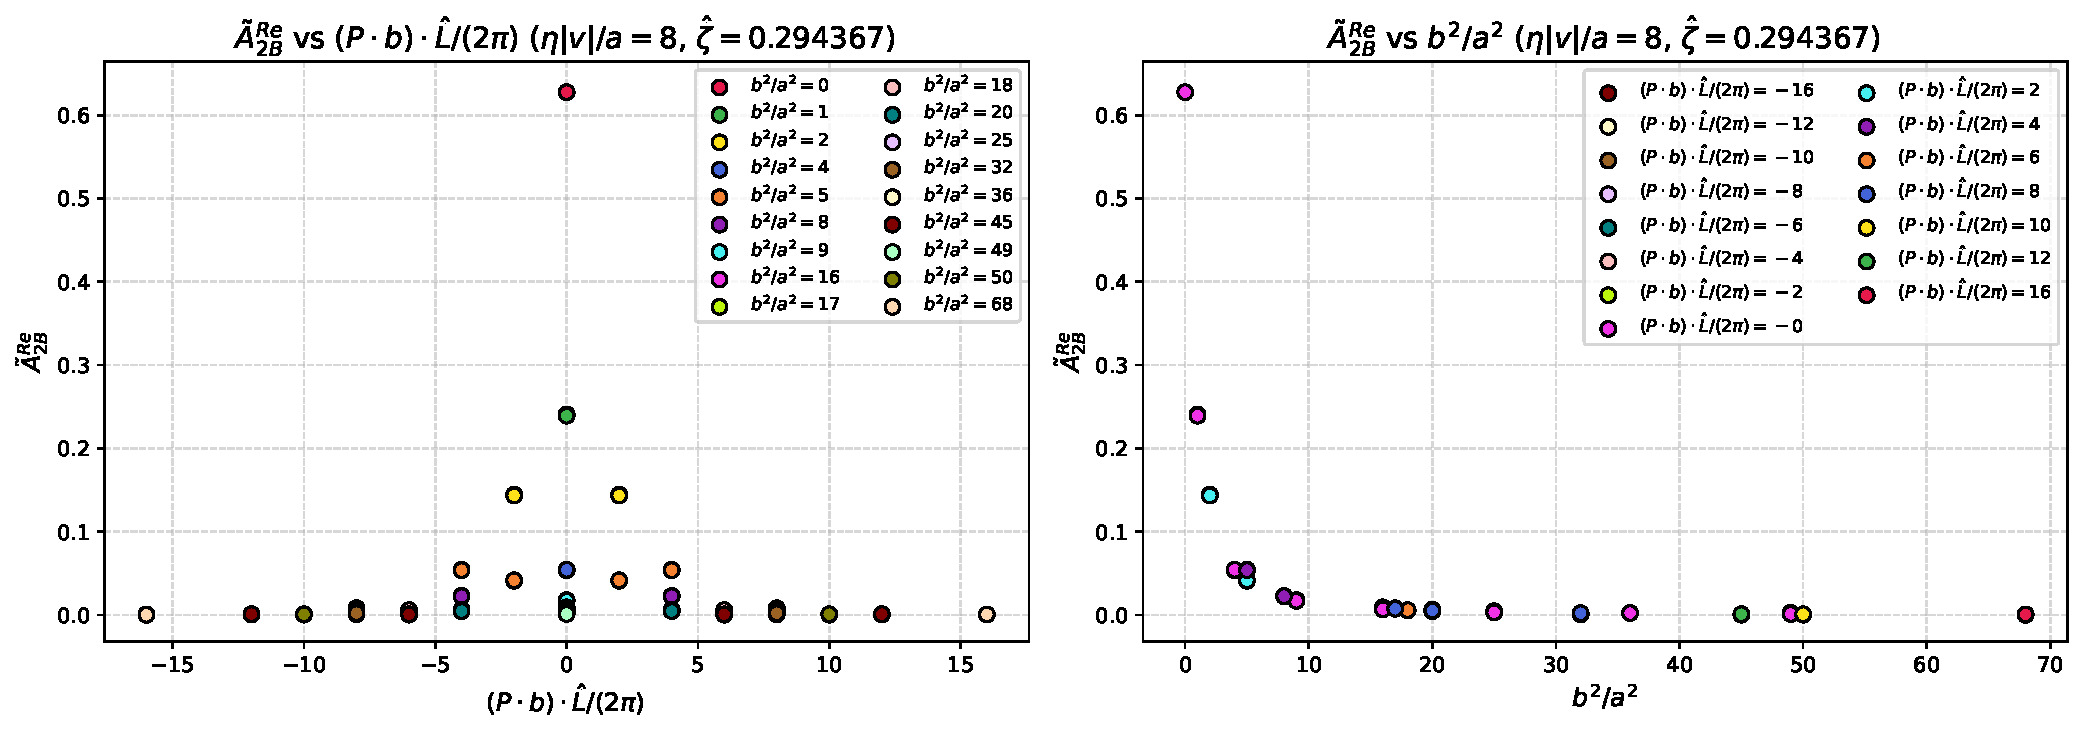
\includegraphics[width=0.98\linewidth,height=0.73\textheight,keepaspectratio]{ReA2B_Pb_bsq_eta8_PL-2_2D.pdf}\\[1mm]
{\small $\zetahat=0.294367$; $(\nu,s)$; $\eta|v|/a=8$ slices}
\figsrc{Thesis, Ch. 5: raw amplitude profiles; complete original panels.}
\end{frame}

\begin{frame}{$\tAmp_{2B}^{\mathrm{Im}}$ at $P_L=-2$: lattice coordinates}
\centering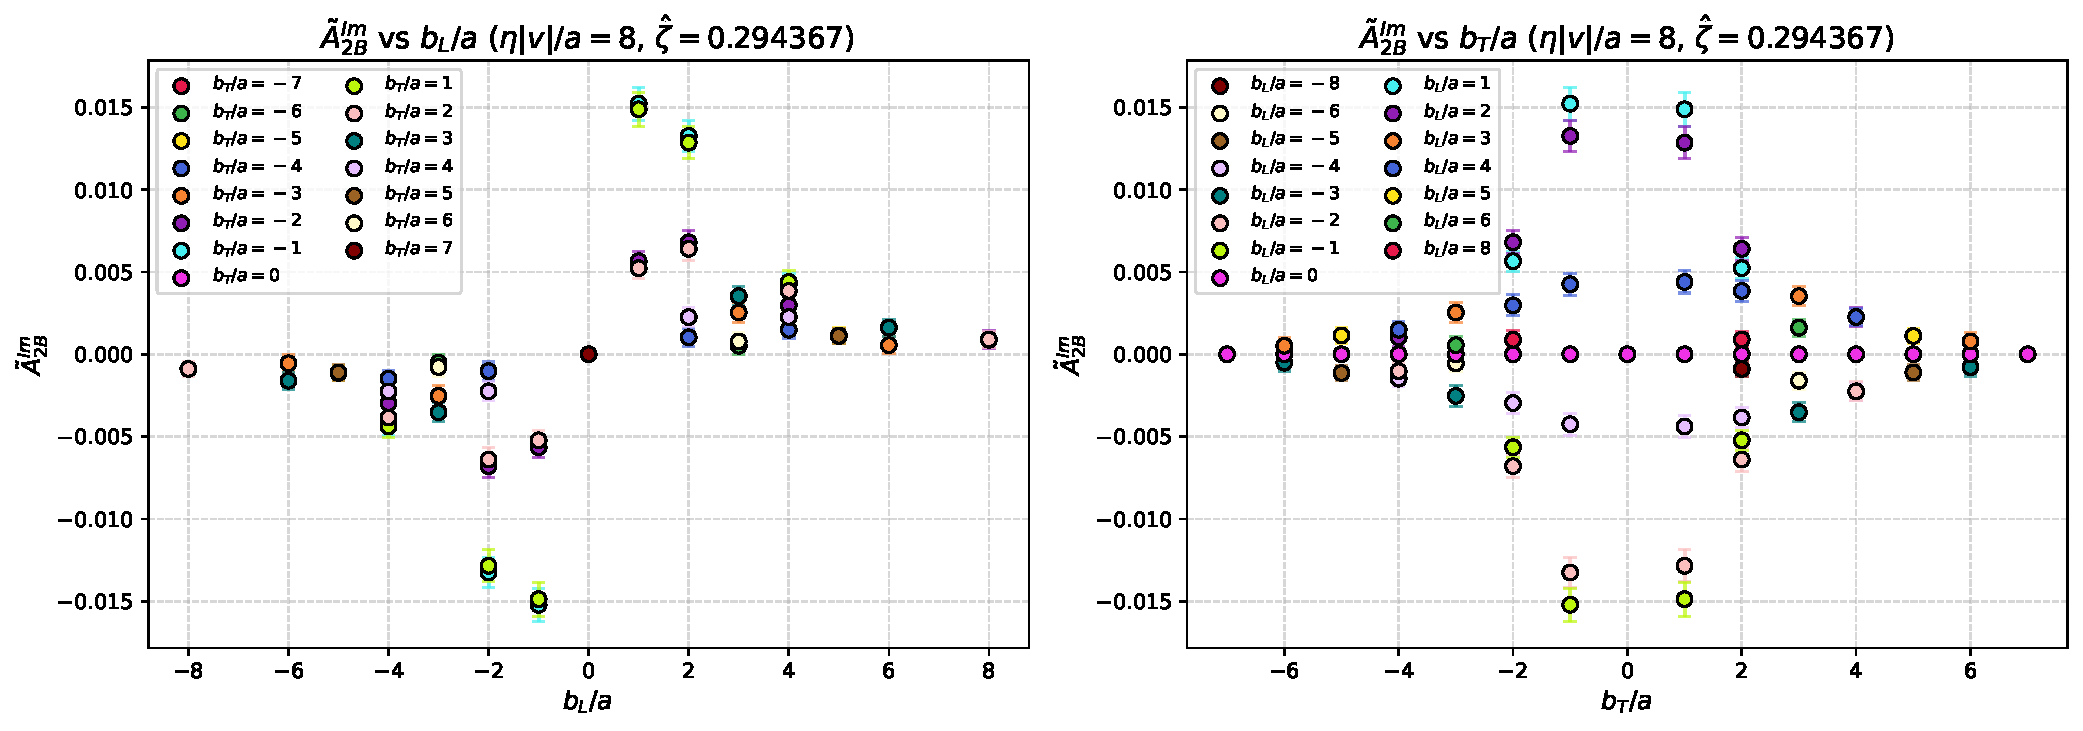
\includegraphics[width=0.98\linewidth,height=0.73\textheight,keepaspectratio]{ImA2B_eta8_PL-2_2D.pdf}\\[1mm]
{\small $\zetahat=0.294367$; $(b_L,b_T)$; $\eta|v|/a=8$ slices}
\figsrc{Thesis, Ch. 5: raw amplitude profiles; complete original panels.}
\end{frame}

\begin{frame}{$\tAmp_{2B}^{\mathrm{Im}}$ at $P_L=-2$: invariant coordinates}
\centering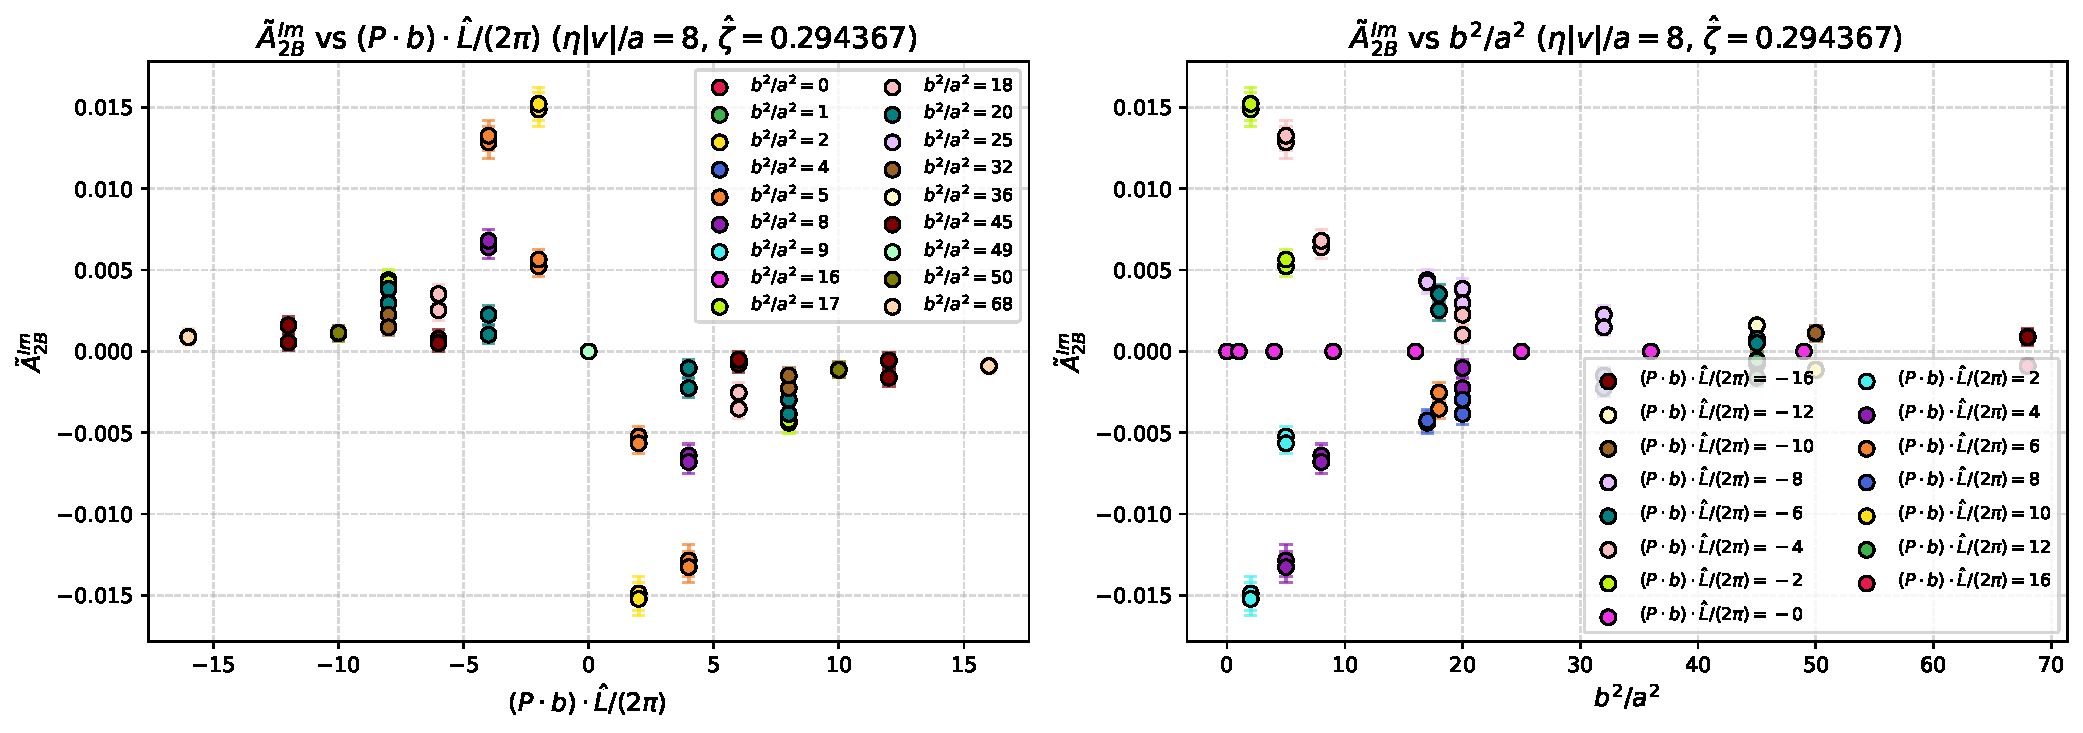
\includegraphics[width=0.98\linewidth,height=0.73\textheight,keepaspectratio]{ImA2B_Pb_bsq_eta8_PL-2_2D.pdf}\\[1mm]
{\small $\zetahat=0.294367$; $(\nu,s)$; $\eta|v|/a=8$ slices}
\figsrc{Thesis, Ch. 5: raw amplitude profiles; complete original panels.}
\end{frame}

\begin{frame}{$\tAmp_{12B}^{\mathrm{Re}}$ at $P_L=-2$: lattice coordinates}
\centering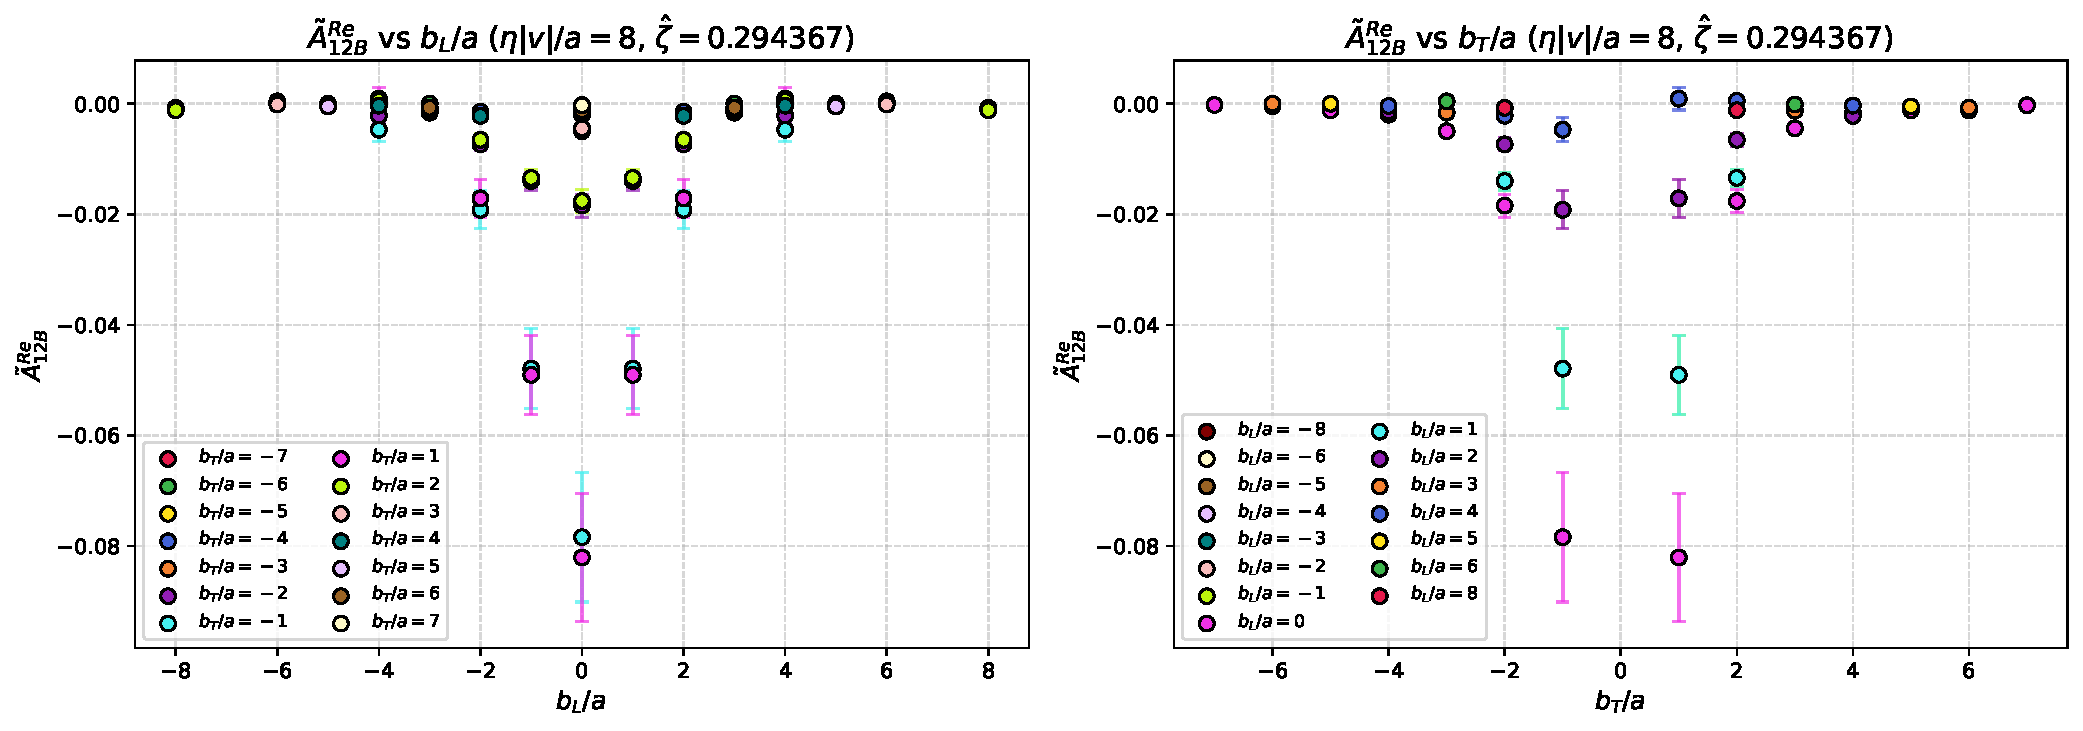
\includegraphics[width=0.98\linewidth,height=0.73\textheight,keepaspectratio]{ReA12B_eta8_PL-2_2D.pdf}\\[1mm]
{\small $\zetahat=0.294367$; $(b_L,b_T)$; $\eta|v|/a=8$ slices}
\figsrc{Thesis, Ch. 5: raw amplitude profiles; complete original panels.}
\end{frame}

\begin{frame}{$\tAmp_{12B}^{\mathrm{Re}}$ at $P_L=-2$: invariant coordinates}
\centering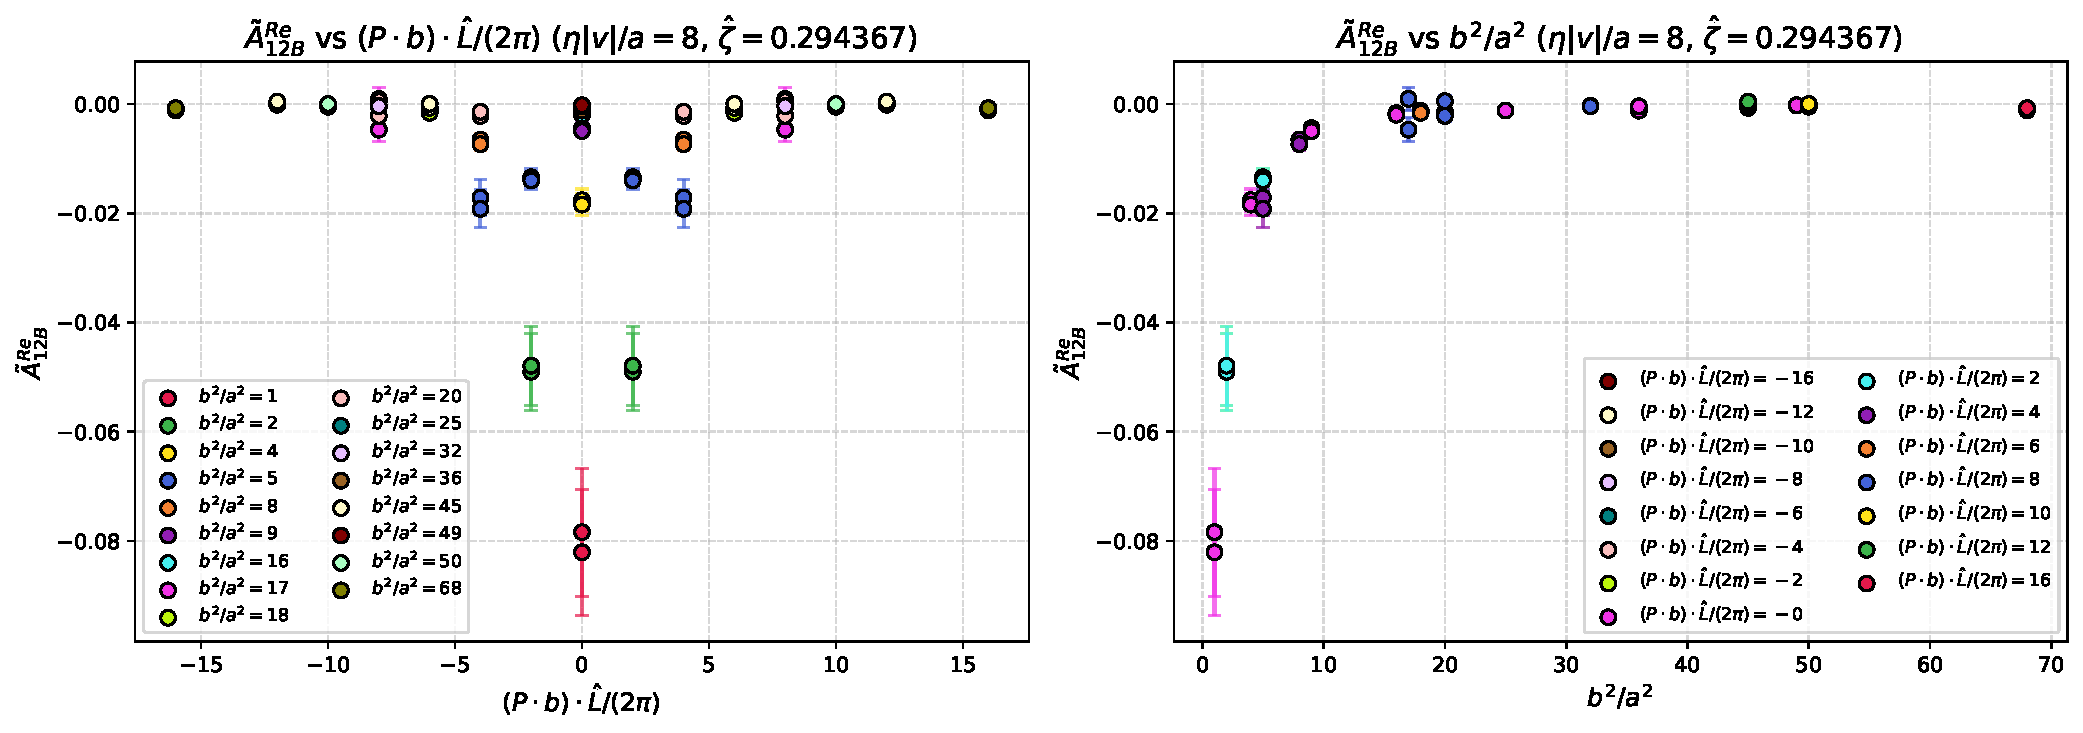
\includegraphics[width=0.98\linewidth,height=0.73\textheight,keepaspectratio]{ReA12B_Pb_bsq_eta8_PL-2_2D.pdf}\\[1mm]
{\small $\zetahat=0.294367$; $(\nu,s)$; $\eta|v|/a=8$ slices}
\figsrc{Thesis, Ch. 5: raw amplitude profiles; complete original panels.}
\end{frame}

\begin{frame}{$\tAmp_{12B}^{\mathrm{Im}}$ at $P_L=-2$: lattice coordinates}
\centering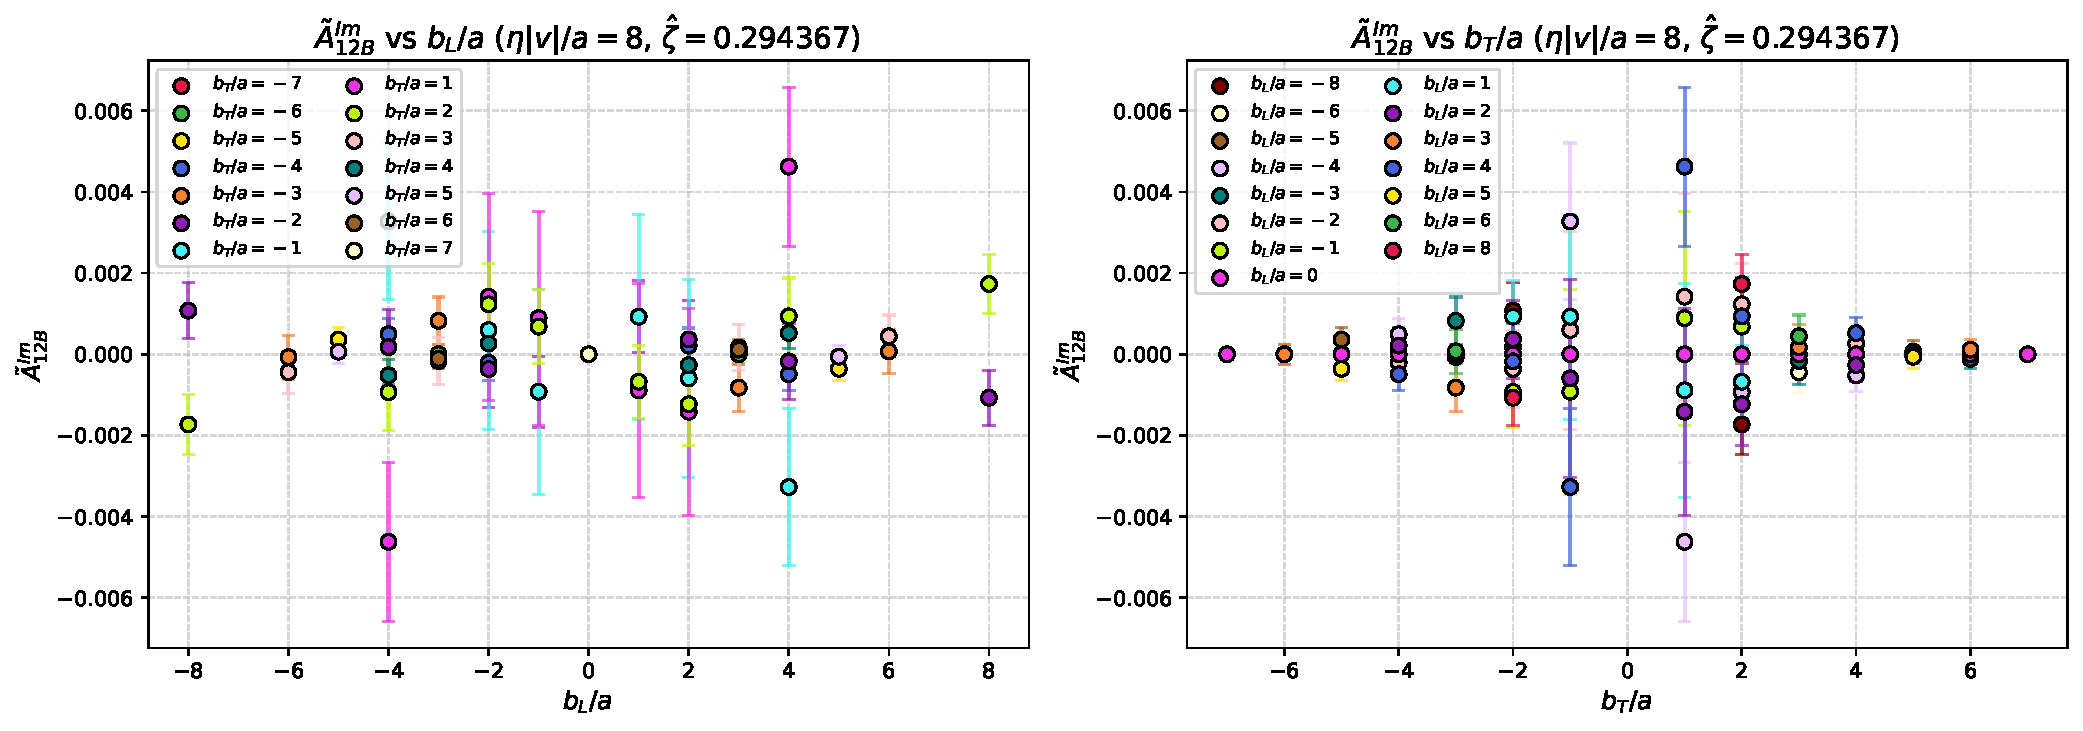
\includegraphics[width=0.98\linewidth,height=0.73\textheight,keepaspectratio]{ImA12B_eta8_PL-2_2D.pdf}\\[1mm]
{\small $\zetahat=0.294367$; $(b_L,b_T)$; $\eta|v|/a=8$ slices}
\figsrc{Thesis, Ch. 5: raw amplitude profiles; complete original panels.}
\end{frame}

\begin{frame}{$\tAmp_{12B}^{\mathrm{Im}}$ at $P_L=-2$: invariant coordinates}
\centering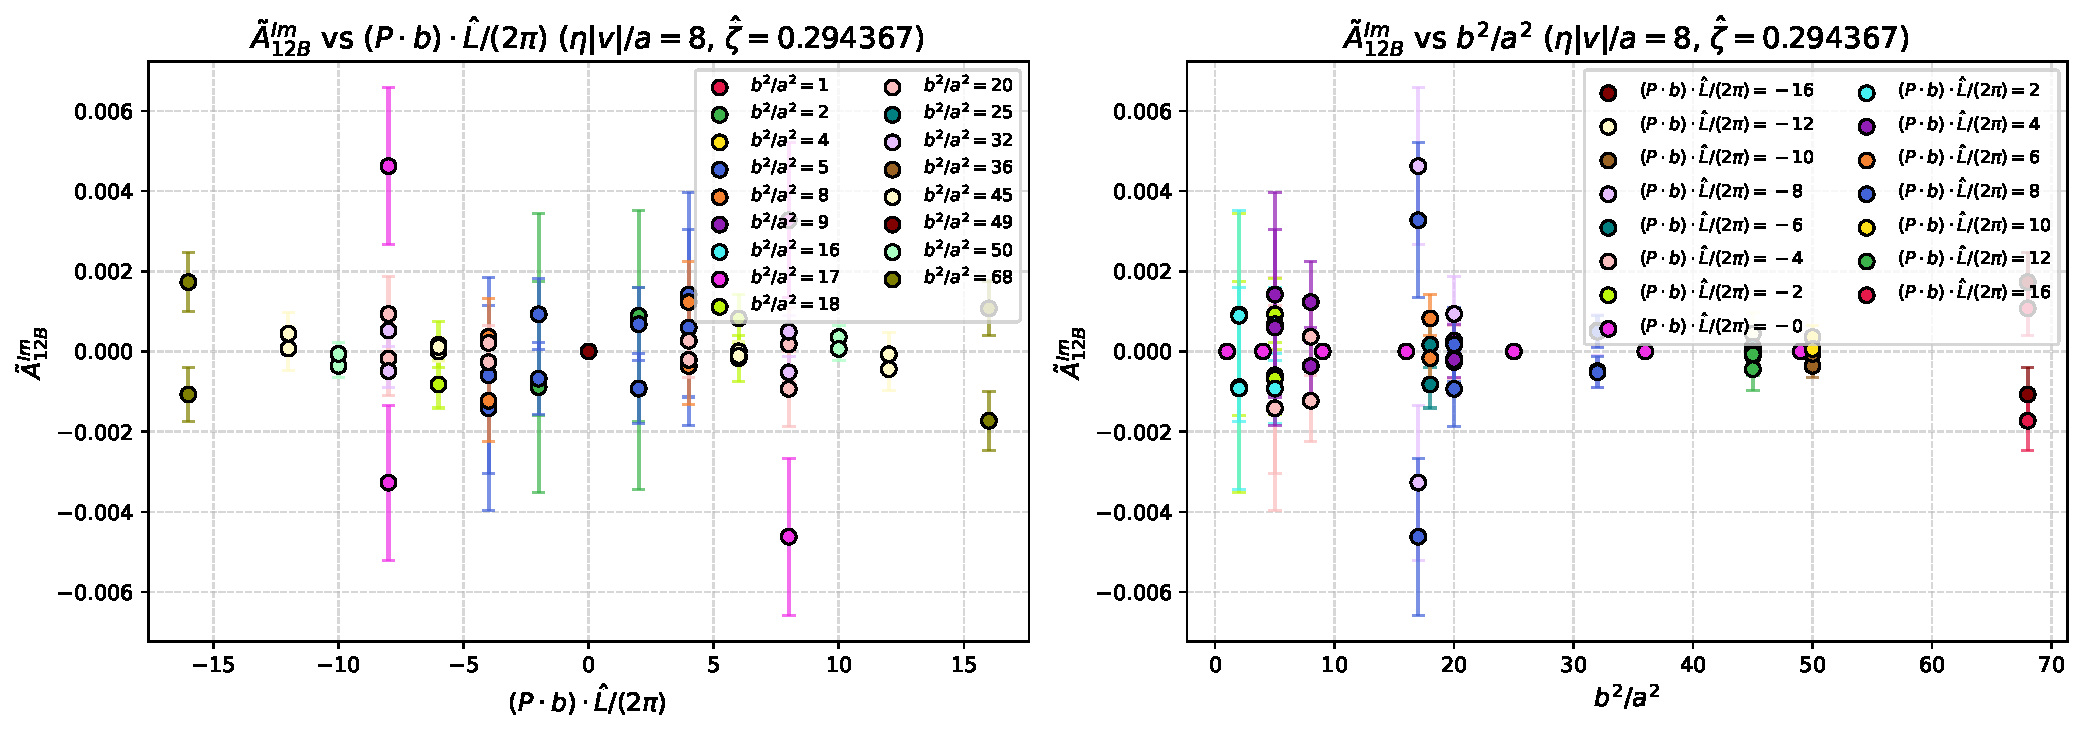
\includegraphics[width=0.98\linewidth,height=0.73\textheight,keepaspectratio]{ImA12B_Pb_bsq_eta8_PL-2_2D.pdf}\\[1mm]
{\small $\zetahat=0.294367$; $(\nu,s)$; $\eta|v|/a=8$ slices}
\figsrc{Thesis, Ch. 5: raw amplitude profiles; complete original panels.}
\end{frame}

\begin{frame}{$\tAmp_{2B}^{\mathrm{Re}}$ at $P_L=-3$: lattice coordinates}
\centering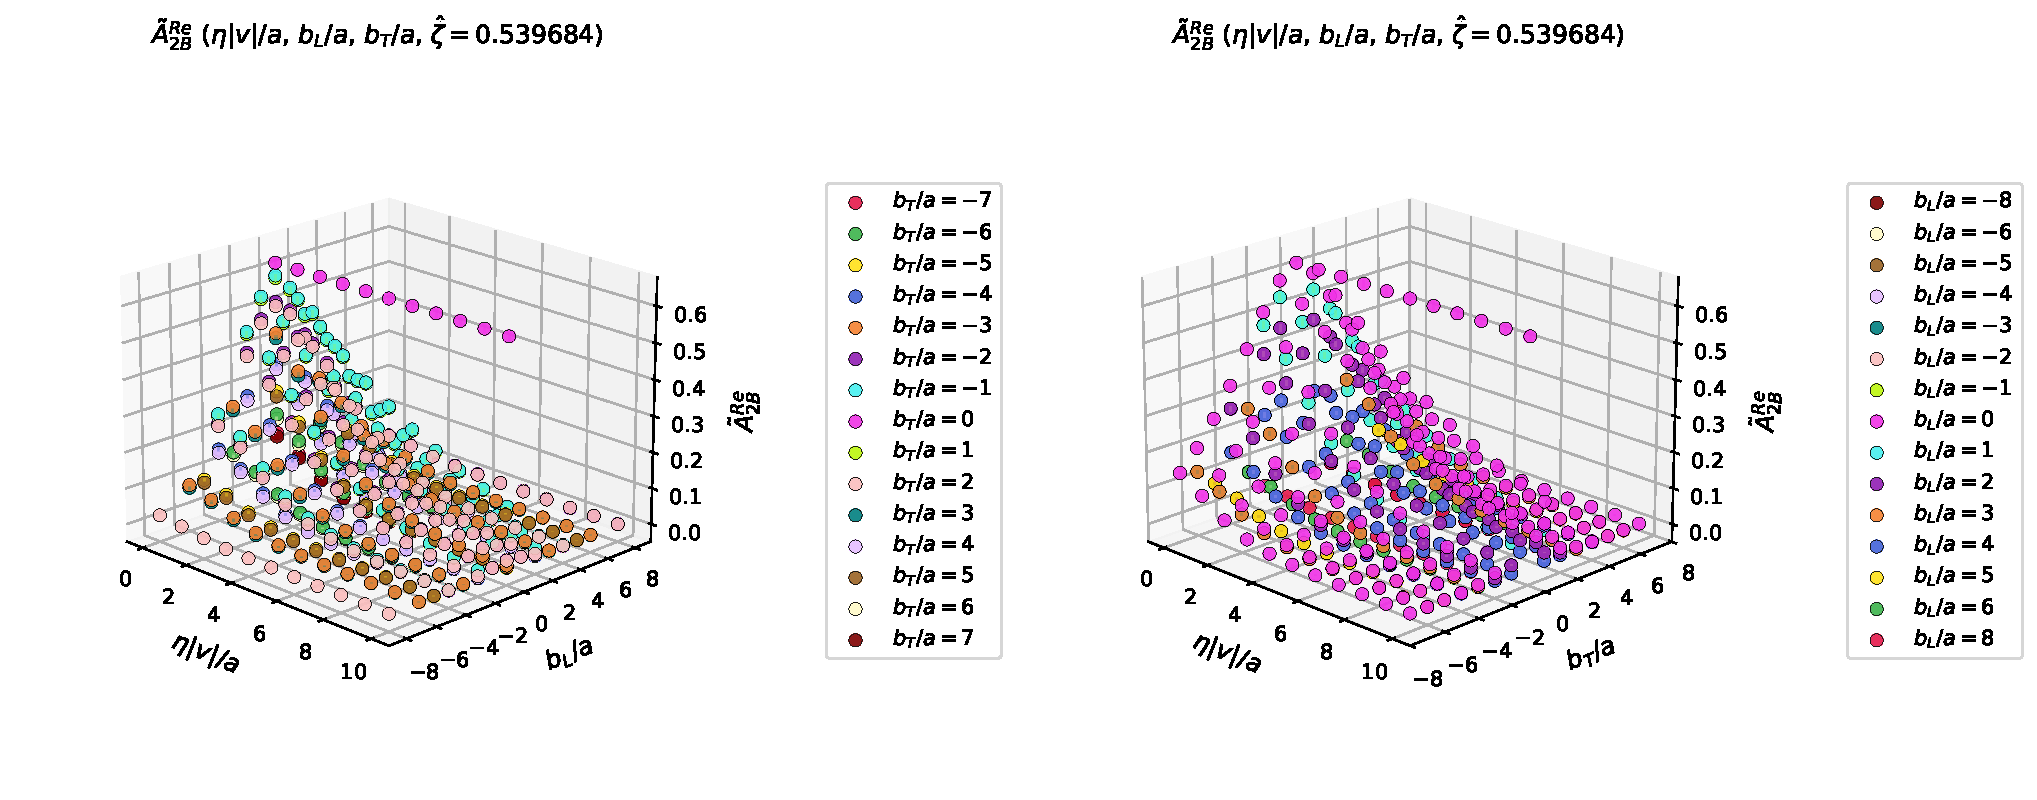
\includegraphics[width=0.98\linewidth,height=0.73\textheight,keepaspectratio]{ReA2B_PL-3_3D.pdf}\\[1mm]
{\small $\zetahat=0.539684$; $(b_L,b_T)$; staple-length dependence}
\figsrc{Thesis, Ch. 5: raw amplitude profiles; complete original panels.}
\end{frame}

\begin{frame}{$\tAmp_{2B}^{\mathrm{Re}}$ at $P_L=-3$: invariant coordinates}
\centering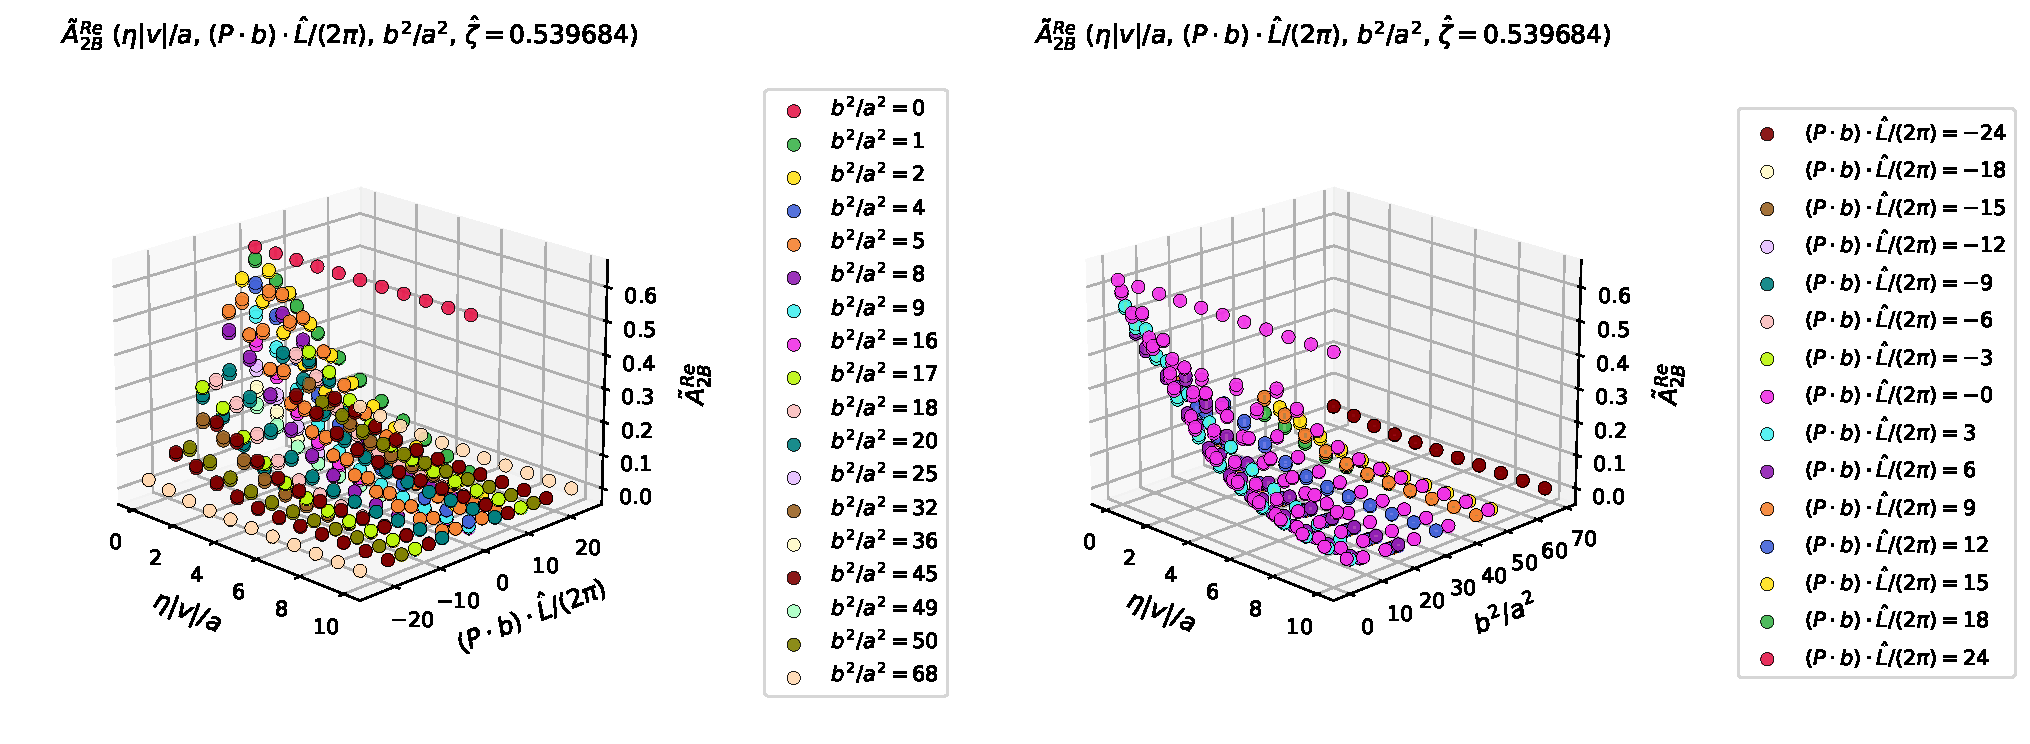
\includegraphics[width=0.98\linewidth,height=0.73\textheight,keepaspectratio]{ReA2B_Pb_bsq_PL-3_3D.pdf}\\[1mm]
{\small $\zetahat=0.539684$; $(\nu,s)$; staple-length dependence}
\figsrc{Thesis, Ch. 5: raw amplitude profiles; complete original panels.}
\end{frame}

\begin{frame}{$\tAmp_{2B}^{\mathrm{Im}}$ at $P_L=-3$: lattice coordinates}
\centering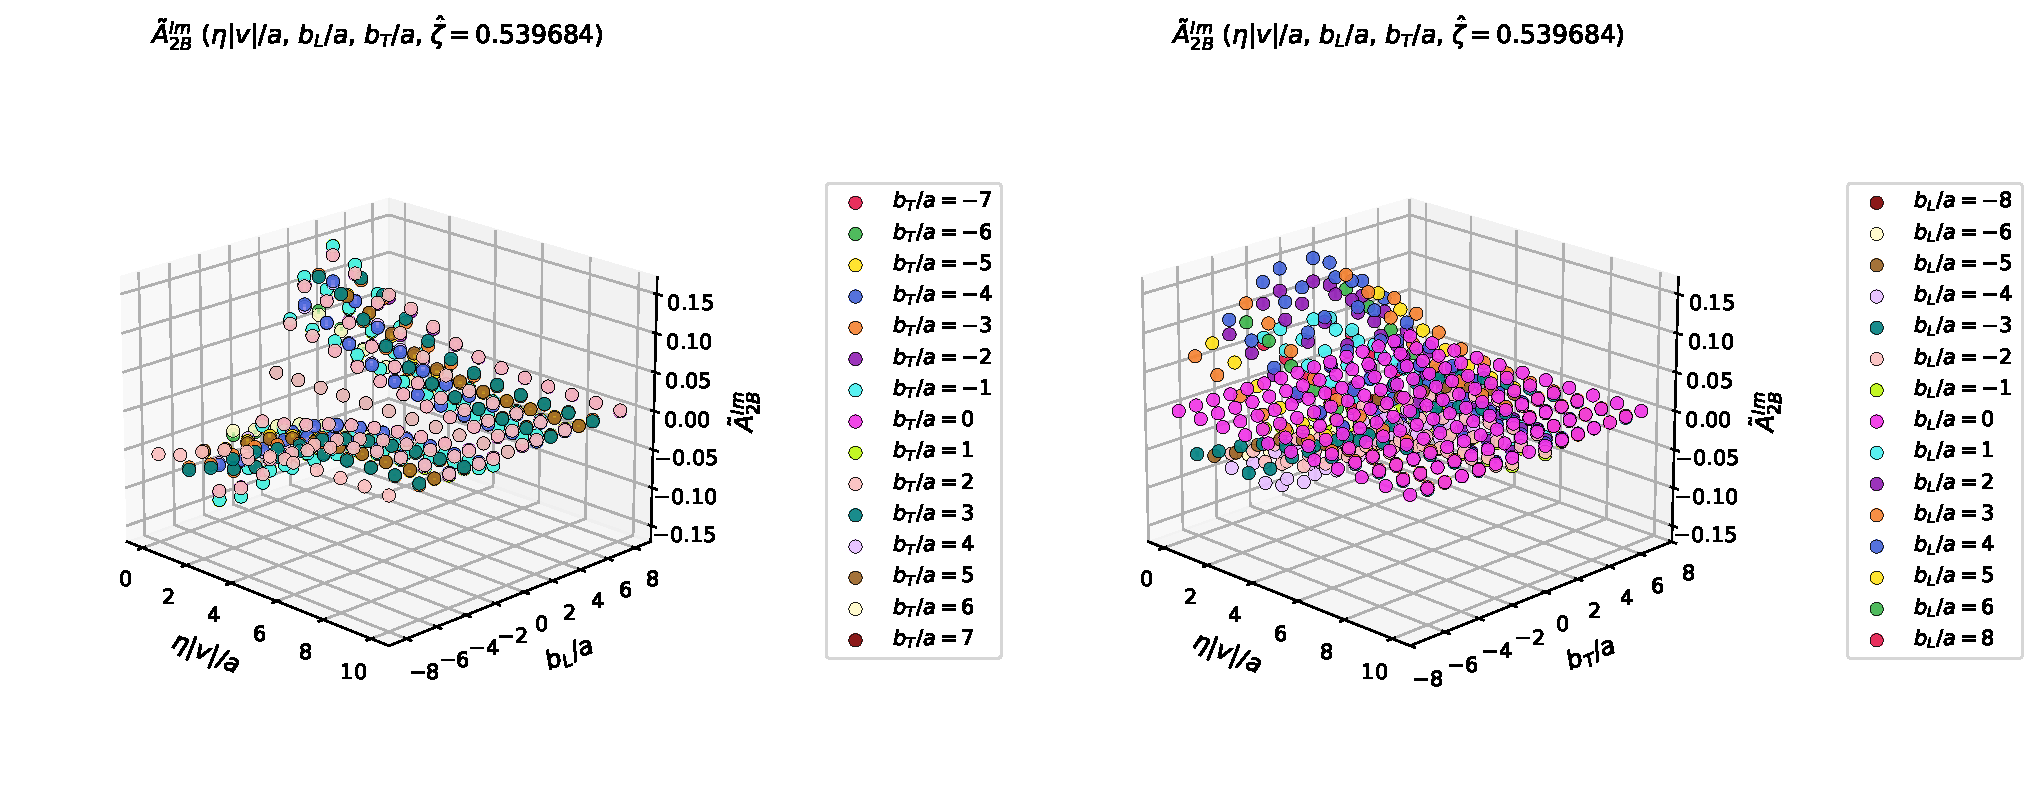
\includegraphics[width=0.98\linewidth,height=0.73\textheight,keepaspectratio]{ImA2B_PL-3_3D.pdf}\\[1mm]
{\small $\zetahat=0.539684$; $(b_L,b_T)$; staple-length dependence}
\figsrc{Thesis, Ch. 5: raw amplitude profiles; complete original panels.}
\end{frame}

\begin{frame}{$\tAmp_{2B}^{\mathrm{Im}}$ at $P_L=-3$: invariant coordinates}
\centering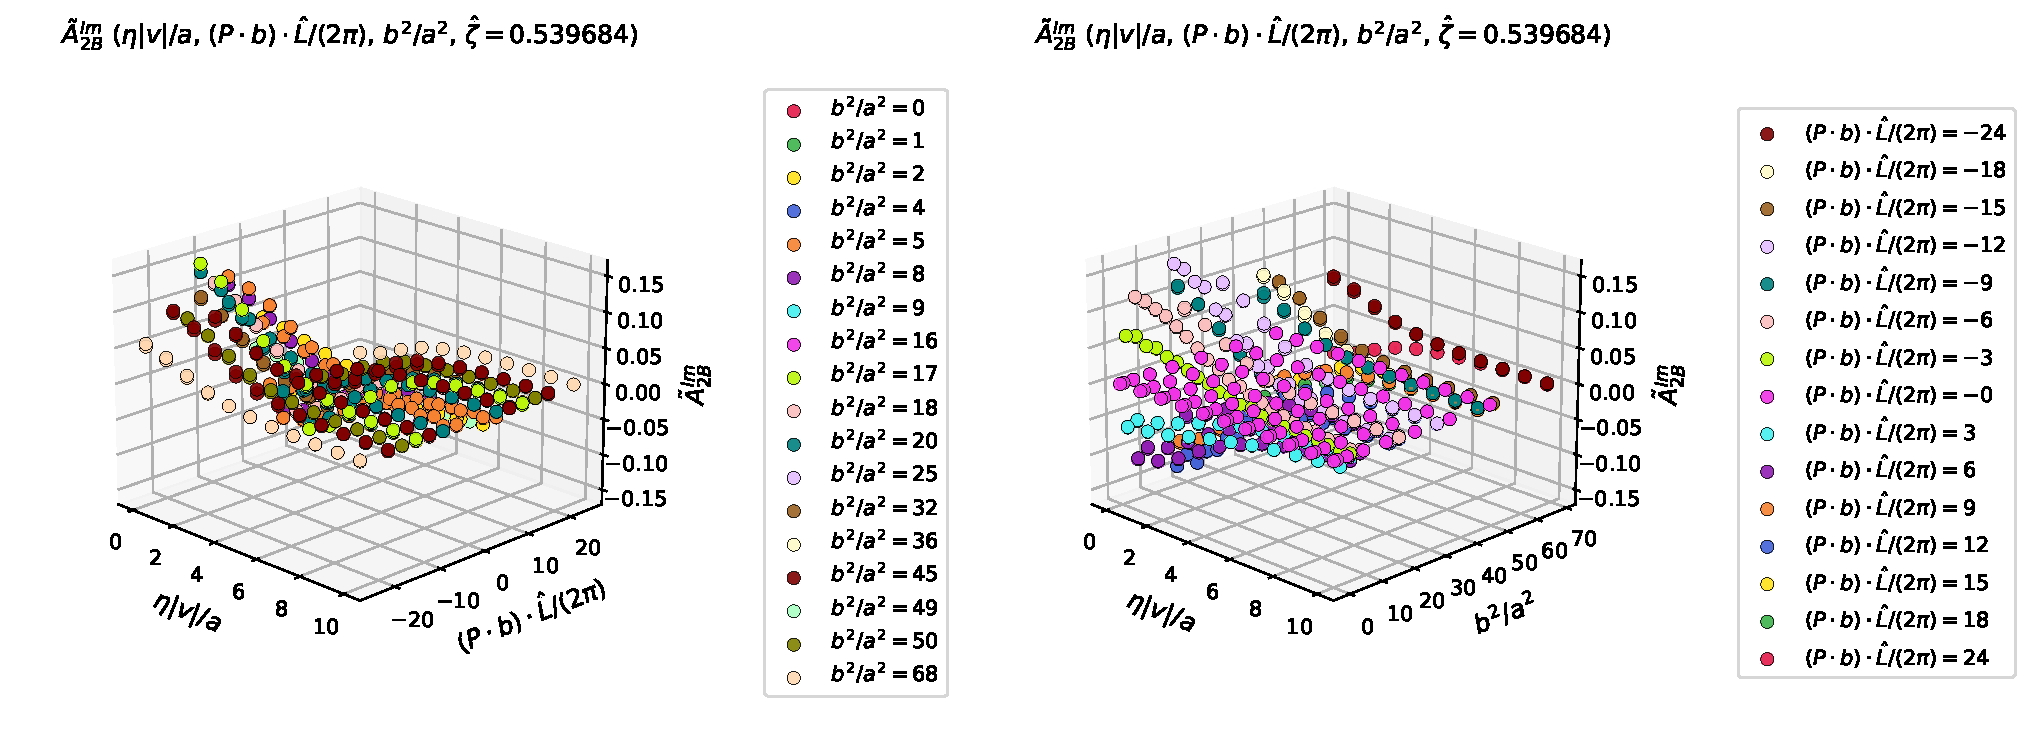
\includegraphics[width=0.98\linewidth,height=0.73\textheight,keepaspectratio]{ImA2B_Pb_bsq_PL-3_3D.pdf}\\[1mm]
{\small $\zetahat=0.539684$; $(\nu,s)$; staple-length dependence}
\figsrc{Thesis, Ch. 5: raw amplitude profiles; complete original panels.}
\end{frame}

\begin{frame}{$\tAmp_{12B}^{\mathrm{Re}}$ at $P_L=-3$: lattice coordinates}
\centering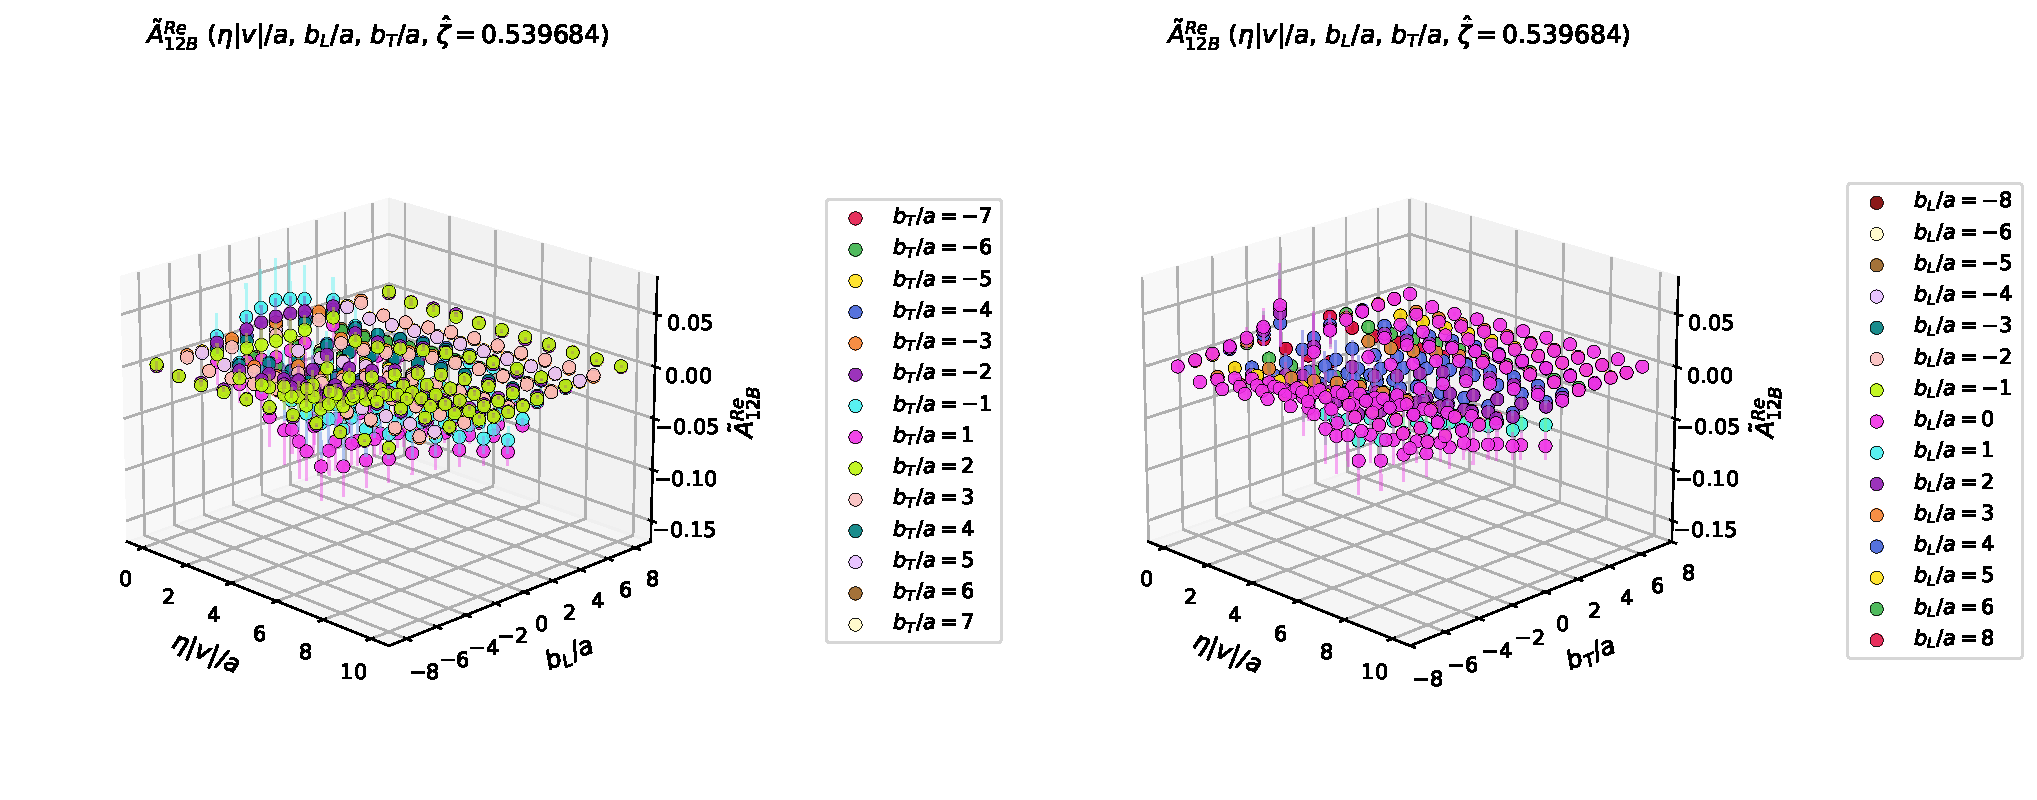
\includegraphics[width=0.98\linewidth,height=0.73\textheight,keepaspectratio]{ReA12B_PL-3_3D.pdf}\\[1mm]
{\small $\zetahat=0.539684$; $(b_L,b_T)$; staple-length dependence}
\figsrc{Thesis, Ch. 5: raw amplitude profiles; complete original panels.}
\end{frame}

\begin{frame}{$\tAmp_{12B}^{\mathrm{Re}}$ at $P_L=-3$: invariant coordinates}
\centering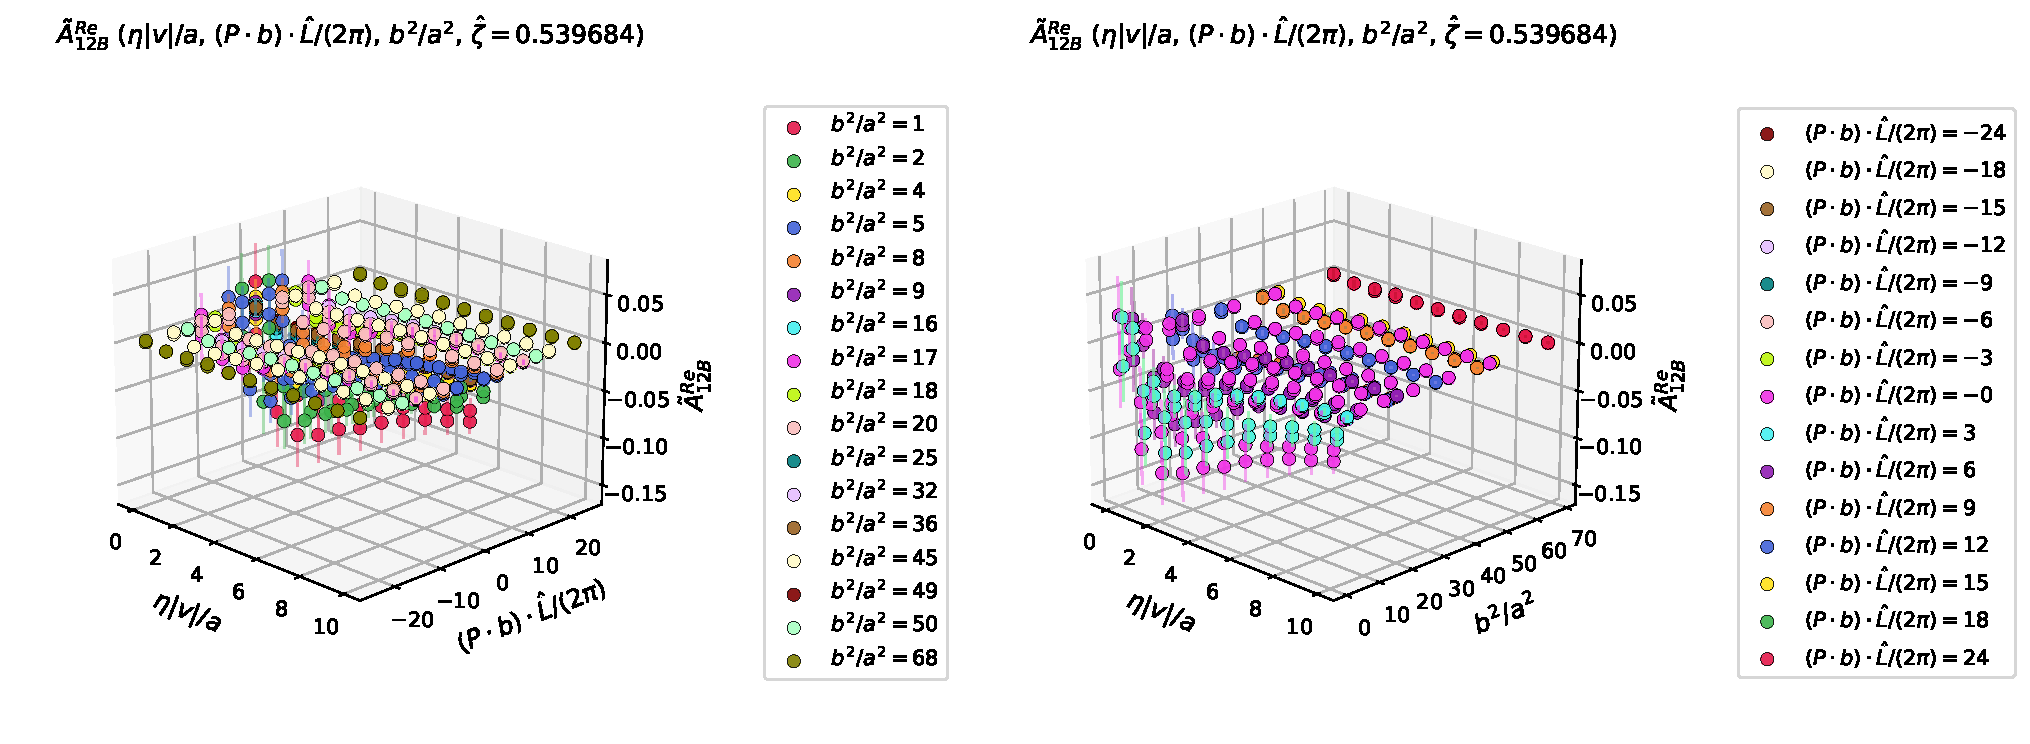
\includegraphics[width=0.98\linewidth,height=0.73\textheight,keepaspectratio]{ReA12B_Pb_bsq_PL-3_3D.pdf}\\[1mm]
{\small $\zetahat=0.539684$; $(\nu,s)$; staple-length dependence}
\figsrc{Thesis, Ch. 5: raw amplitude profiles; complete original panels.}
\end{frame}

\begin{frame}{$\tAmp_{12B}^{\mathrm{Im}}$ at $P_L=-3$: lattice coordinates}
\centering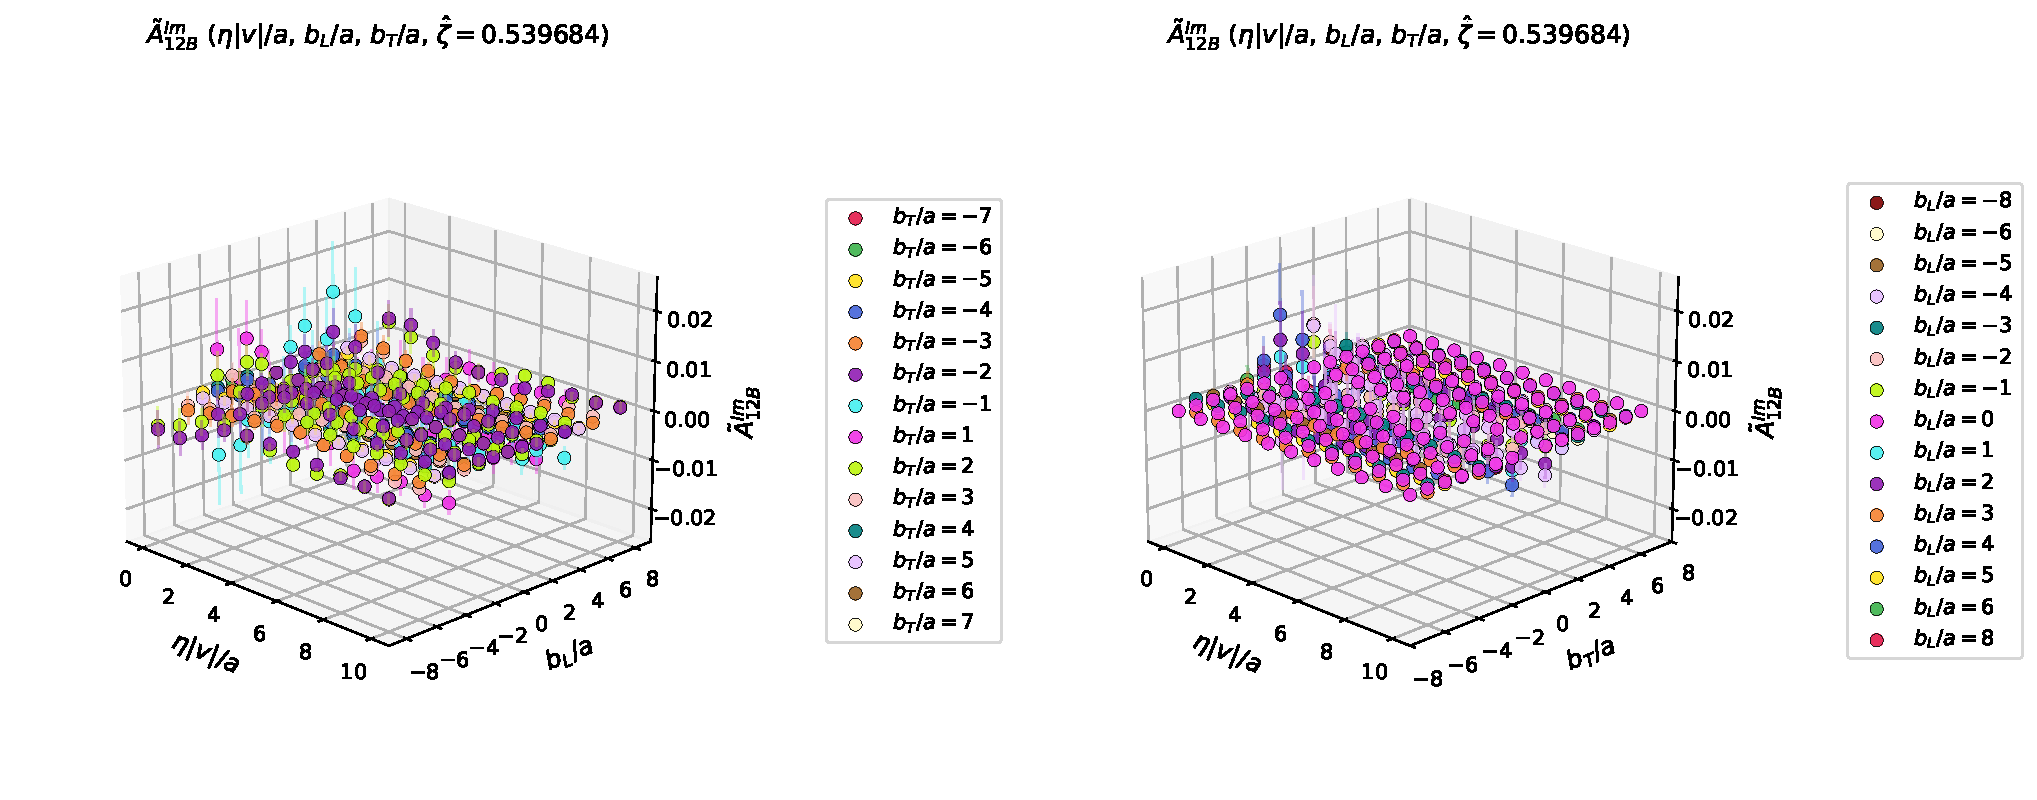
\includegraphics[width=0.98\linewidth,height=0.73\textheight,keepaspectratio]{ImA12B_PL-3_3D.pdf}\\[1mm]
{\small $\zetahat=0.539684$; $(b_L,b_T)$; staple-length dependence}
\figsrc{Thesis, Ch. 5: raw amplitude profiles; complete original panels.}
\end{frame}

\begin{frame}{$\tAmp_{12B}^{\mathrm{Im}}$ at $P_L=-3$: invariant coordinates}
\centering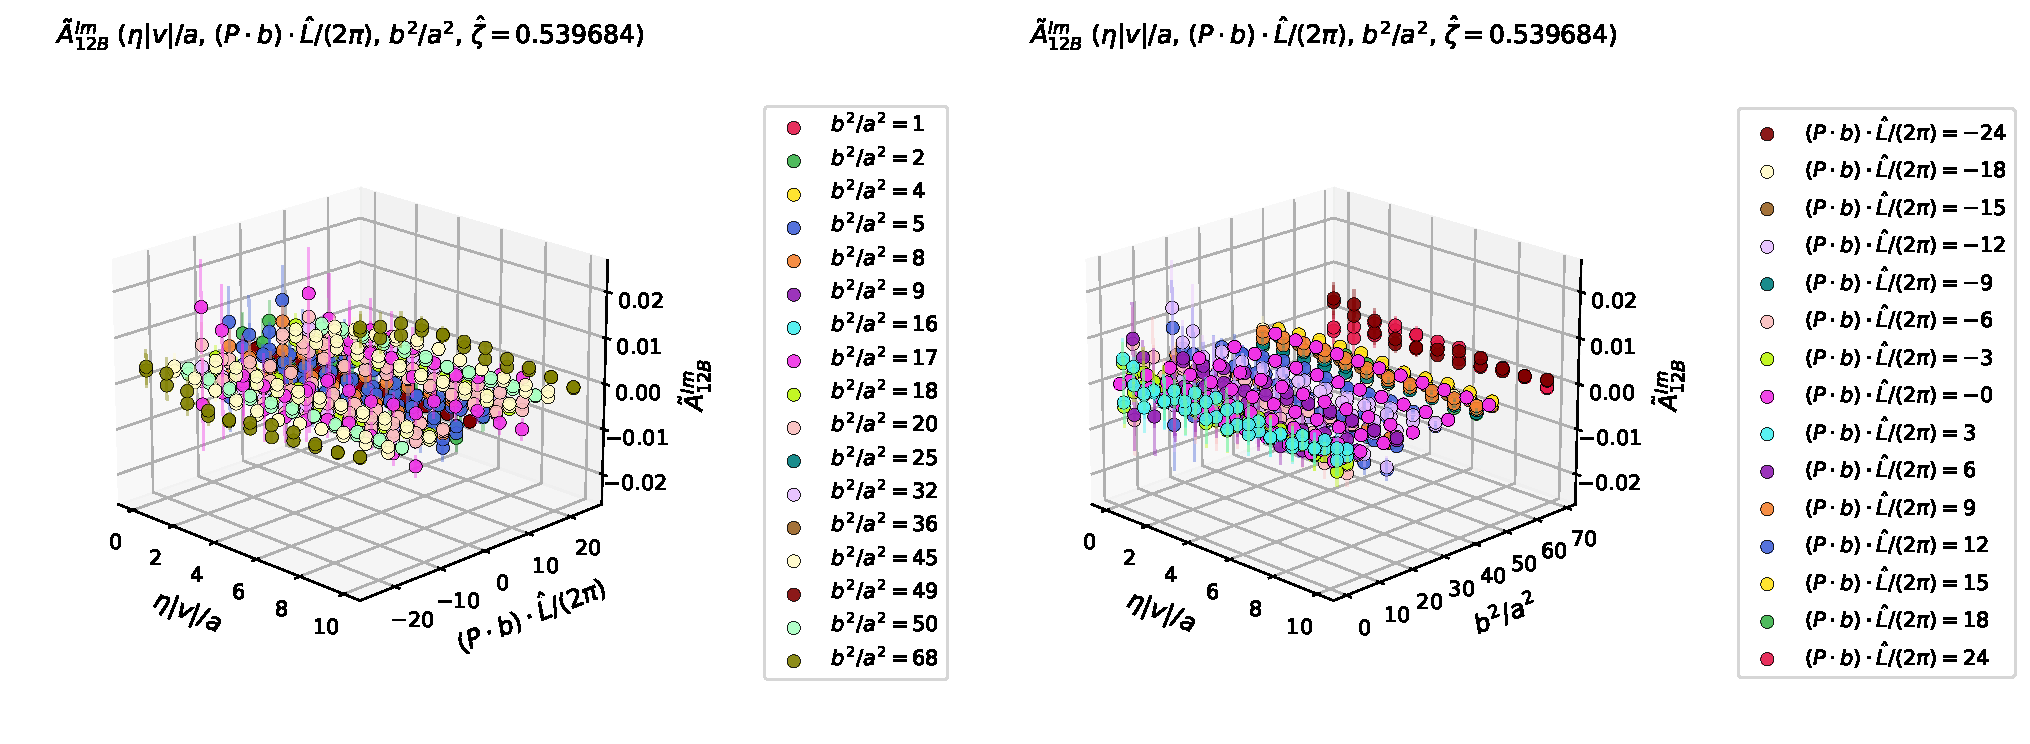
\includegraphics[width=0.98\linewidth,height=0.73\textheight,keepaspectratio]{ImA12B_Pb_bsq_PL-3_3D.pdf}\\[1mm]
{\small $\zetahat=0.539684$; $(\nu,s)$; staple-length dependence}
\figsrc{Thesis, Ch. 5: raw amplitude profiles; complete original panels.}
\end{frame}

\begin{frame}{$\tAmp_{2B}^{\mathrm{Re}}$ at $P_L=-3$: lattice coordinates}
\centering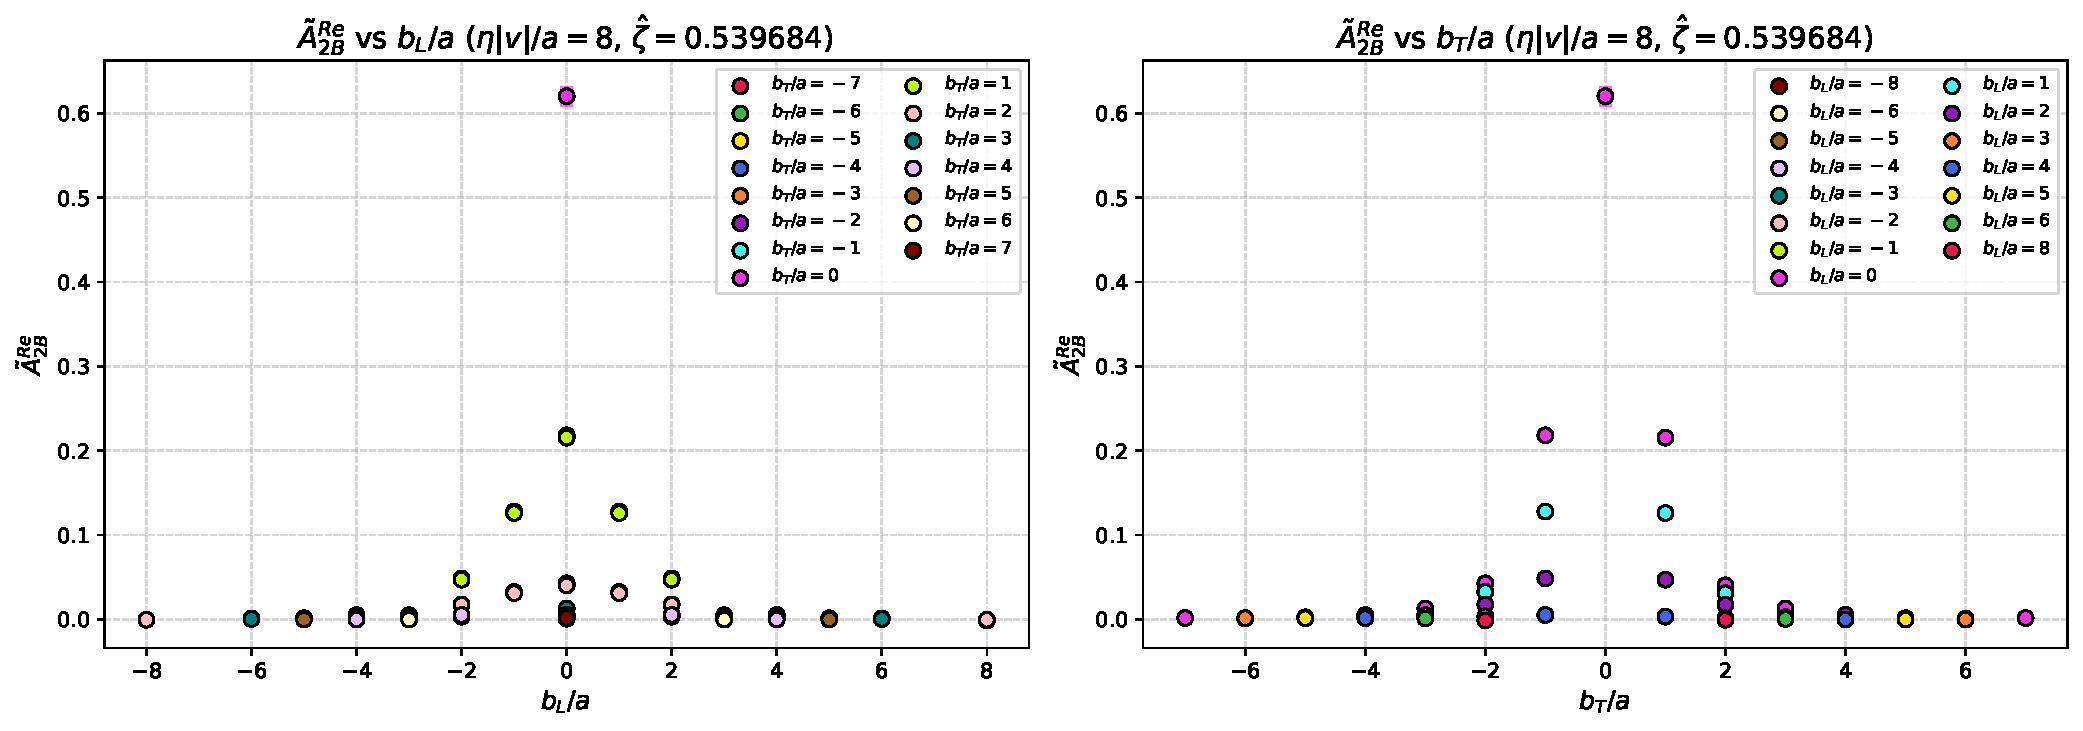
\includegraphics[width=0.98\linewidth,height=0.73\textheight,keepaspectratio]{ReA2B_eta8_PL-3_2D.pdf}\\[1mm]
{\small $\zetahat=0.539684$; $(b_L,b_T)$; $\eta|v|/a=8$ slices}
\figsrc{Thesis, Ch. 5: raw amplitude profiles; complete original panels.}
\end{frame}

\begin{frame}{$\tAmp_{2B}^{\mathrm{Re}}$ at $P_L=-3$: invariant coordinates}
\centering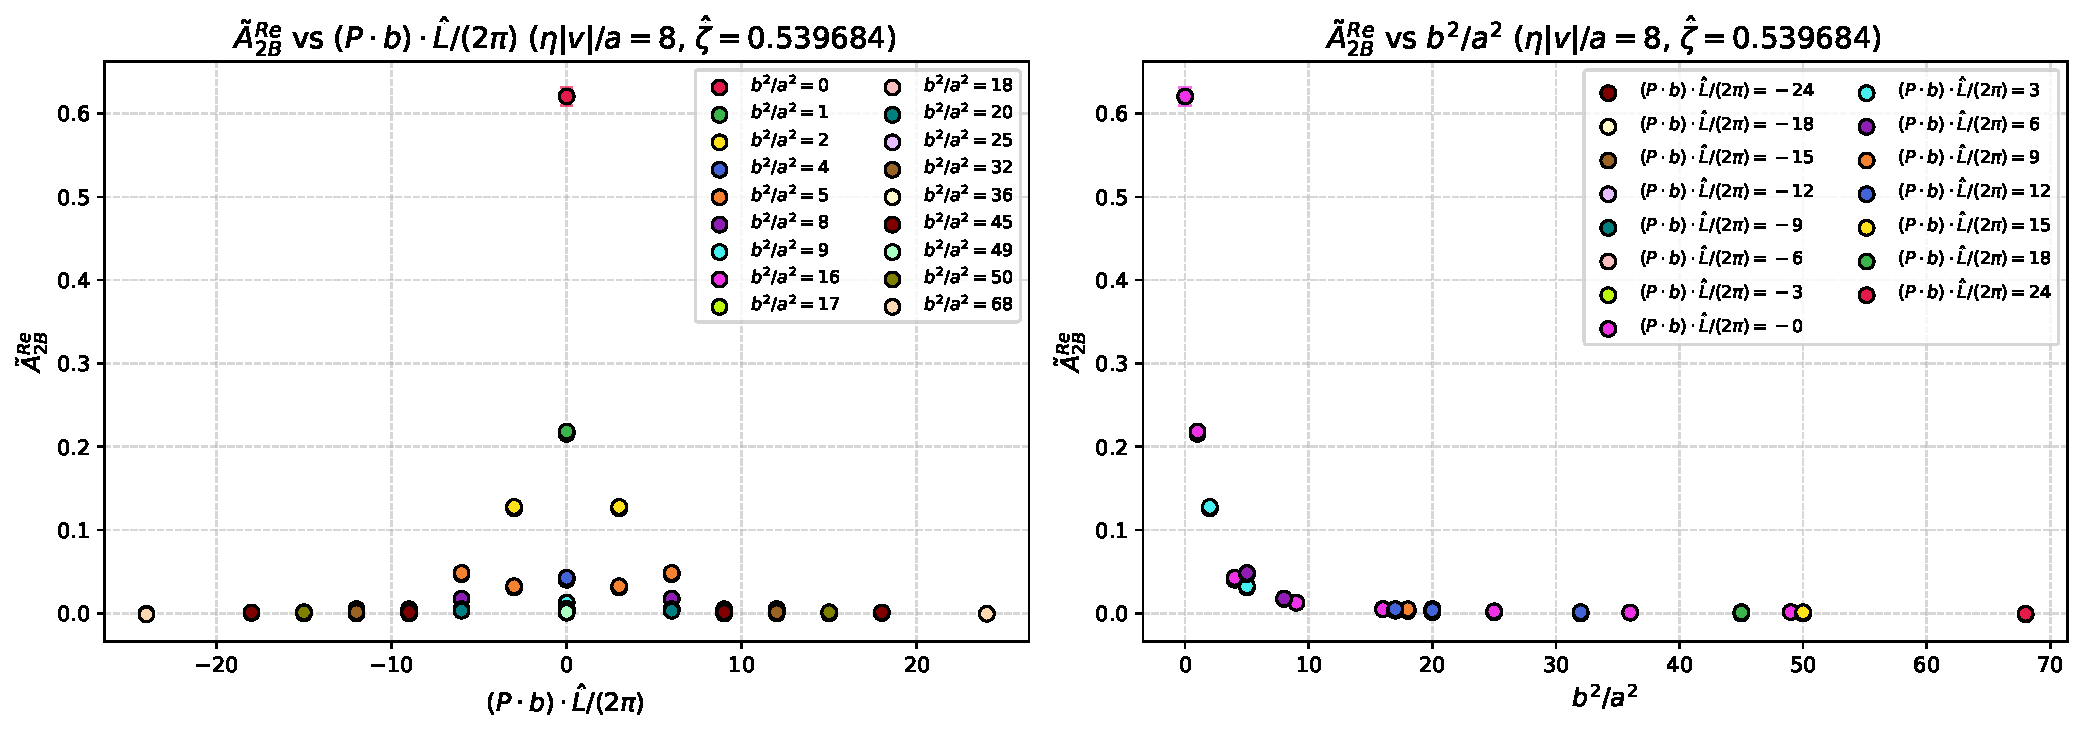
\includegraphics[width=0.98\linewidth,height=0.73\textheight,keepaspectratio]{ReA2B_Pb_bsq_eta8_PL-3_2D.pdf}\\[1mm]
{\small $\zetahat=0.539684$; $(\nu,s)$; $\eta|v|/a=8$ slices}
\figsrc{Thesis, Ch. 5: raw amplitude profiles; complete original panels.}
\end{frame}

\begin{frame}{$\tAmp_{2B}^{\mathrm{Im}}$ at $P_L=-3$: lattice coordinates}
\centering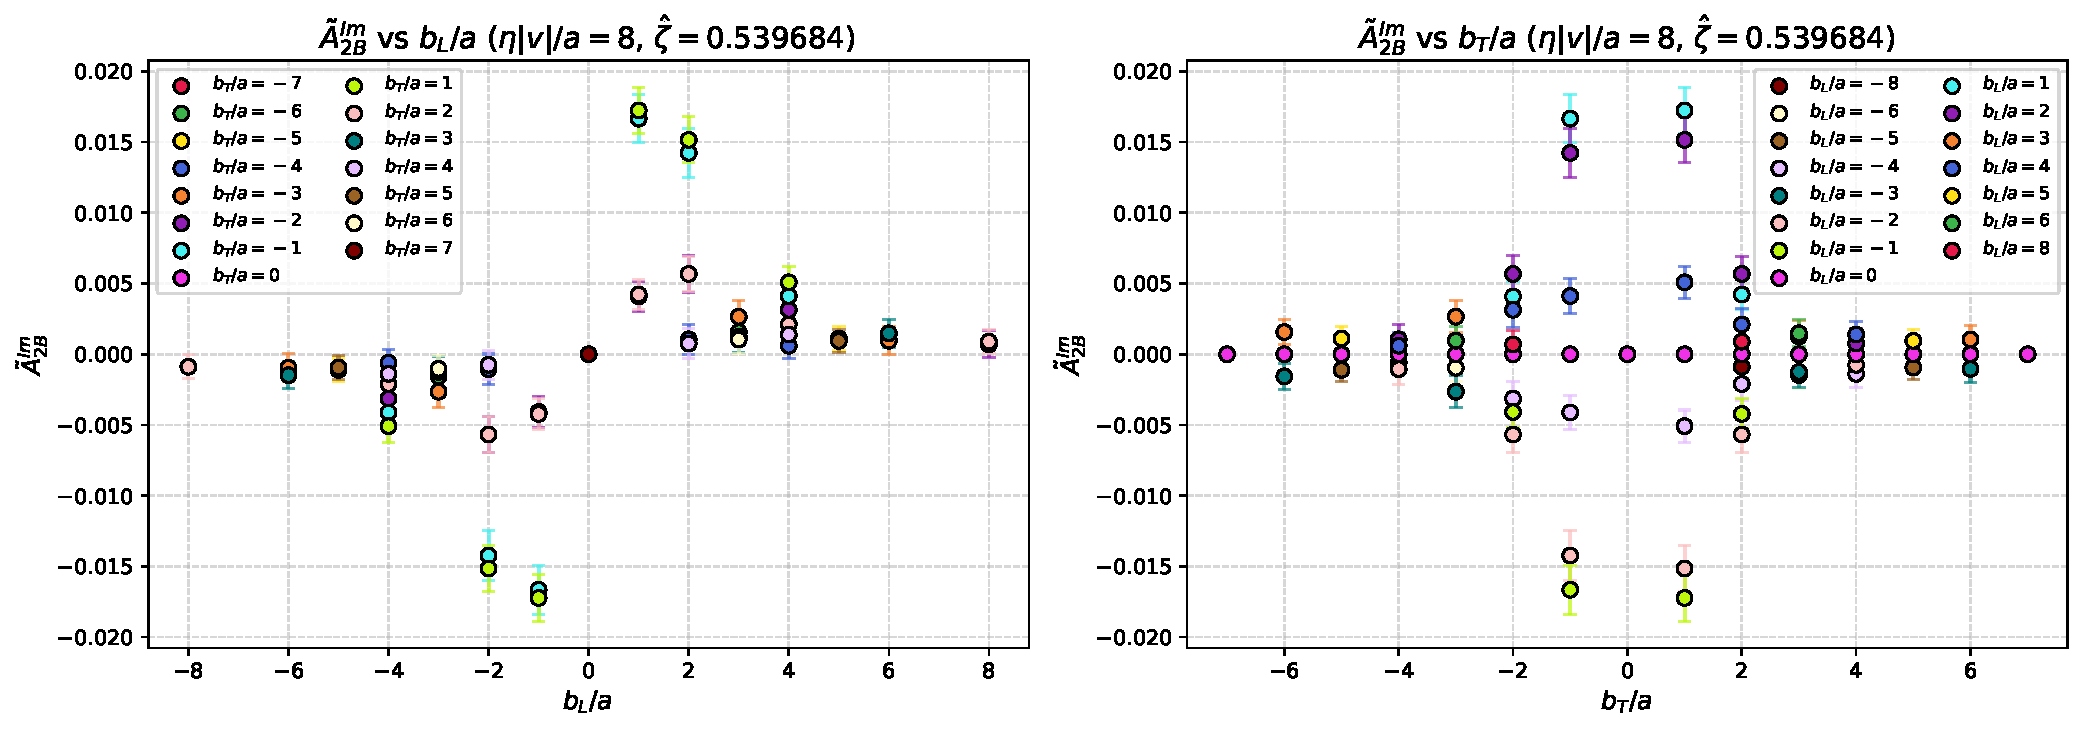
\includegraphics[width=0.98\linewidth,height=0.73\textheight,keepaspectratio]{ImA2B_eta8_PL-3_2D.pdf}\\[1mm]
{\small $\zetahat=0.539684$; $(b_L,b_T)$; $\eta|v|/a=8$ slices}
\figsrc{Thesis, Ch. 5: raw amplitude profiles; complete original panels.}
\end{frame}

\begin{frame}{$\tAmp_{2B}^{\mathrm{Im}}$ at $P_L=-3$: invariant coordinates}
\centering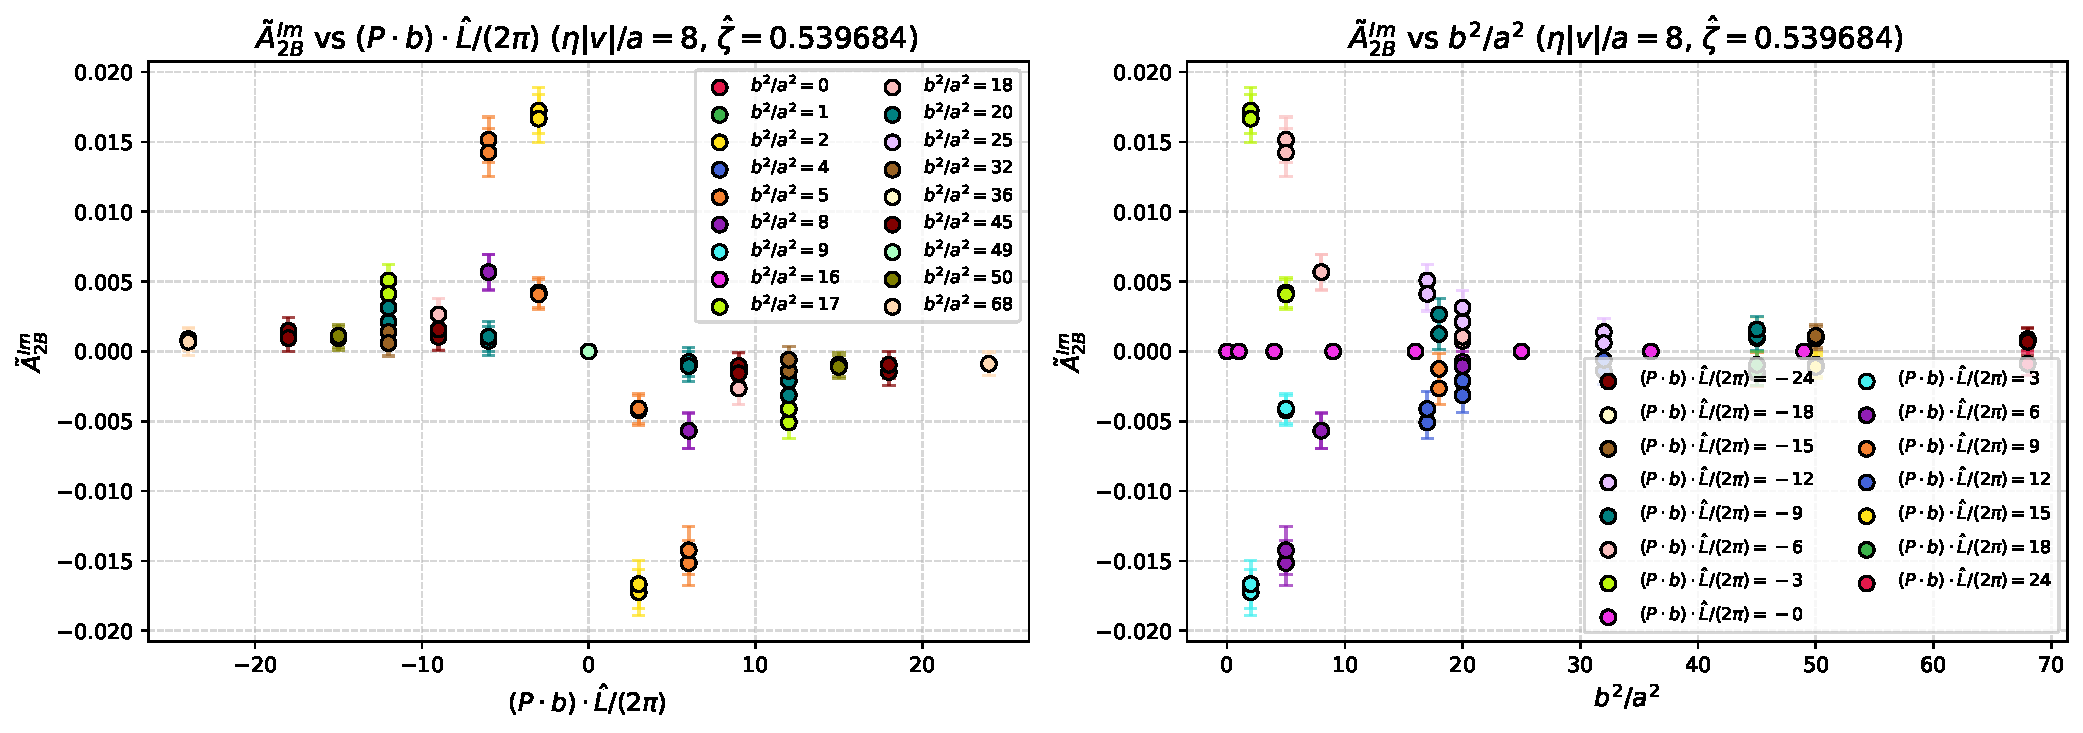
\includegraphics[width=0.98\linewidth,height=0.73\textheight,keepaspectratio]{ImA2B_Pb_bsq_eta8_PL-3_2D.pdf}\\[1mm]
{\small $\zetahat=0.539684$; $(\nu,s)$; $\eta|v|/a=8$ slices}
\figsrc{Thesis, Ch. 5: raw amplitude profiles; complete original panels.}
\end{frame}

\begin{frame}{$\tAmp_{12B}^{\mathrm{Re}}$ at $P_L=-3$: lattice coordinates}
\centering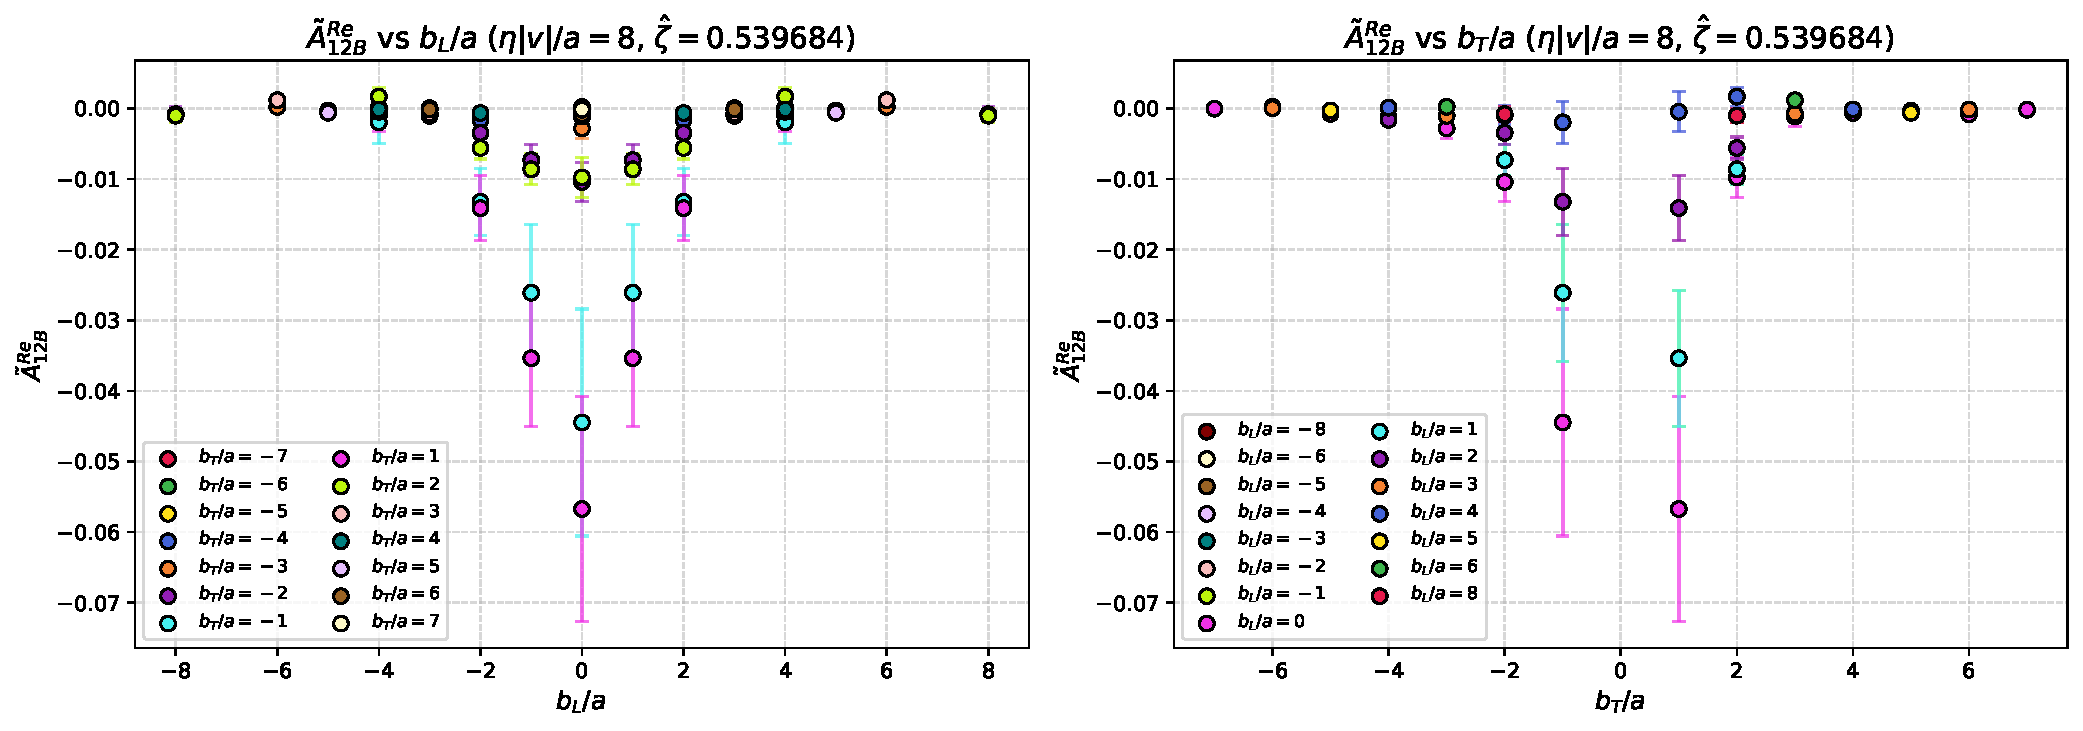
\includegraphics[width=0.98\linewidth,height=0.73\textheight,keepaspectratio]{ReA12B_eta8_PL-3_2D.pdf}\\[1mm]
{\small $\zetahat=0.539684$; $(b_L,b_T)$; $\eta|v|/a=8$ slices}
\figsrc{Thesis, Ch. 5: raw amplitude profiles; complete original panels.}
\end{frame}

\begin{frame}{$\tAmp_{12B}^{\mathrm{Re}}$ at $P_L=-3$: invariant coordinates}
\centering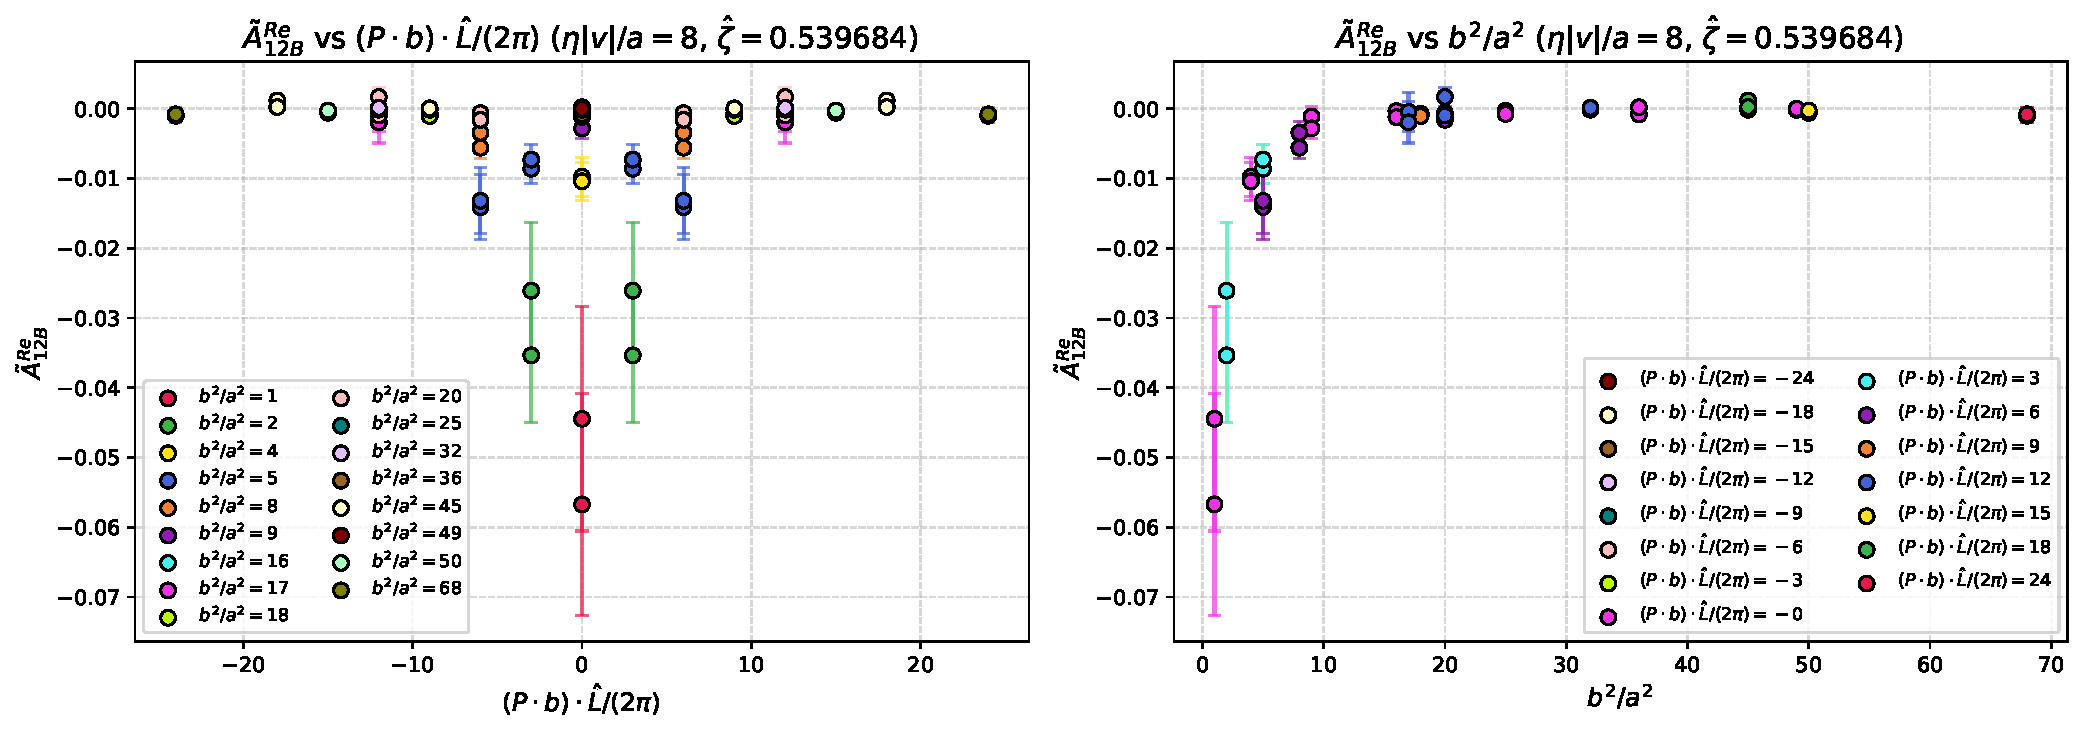
\includegraphics[width=0.98\linewidth,height=0.73\textheight,keepaspectratio]{ReA12B_Pb_bsq_eta8_PL-3_2D.pdf}\\[1mm]
{\small $\zetahat=0.539684$; $(\nu,s)$; $\eta|v|/a=8$ slices}
\figsrc{Thesis, Ch. 5: raw amplitude profiles; complete original panels.}
\end{frame}

\begin{frame}{$\tAmp_{12B}^{\mathrm{Im}}$ at $P_L=-3$: lattice coordinates}
\centering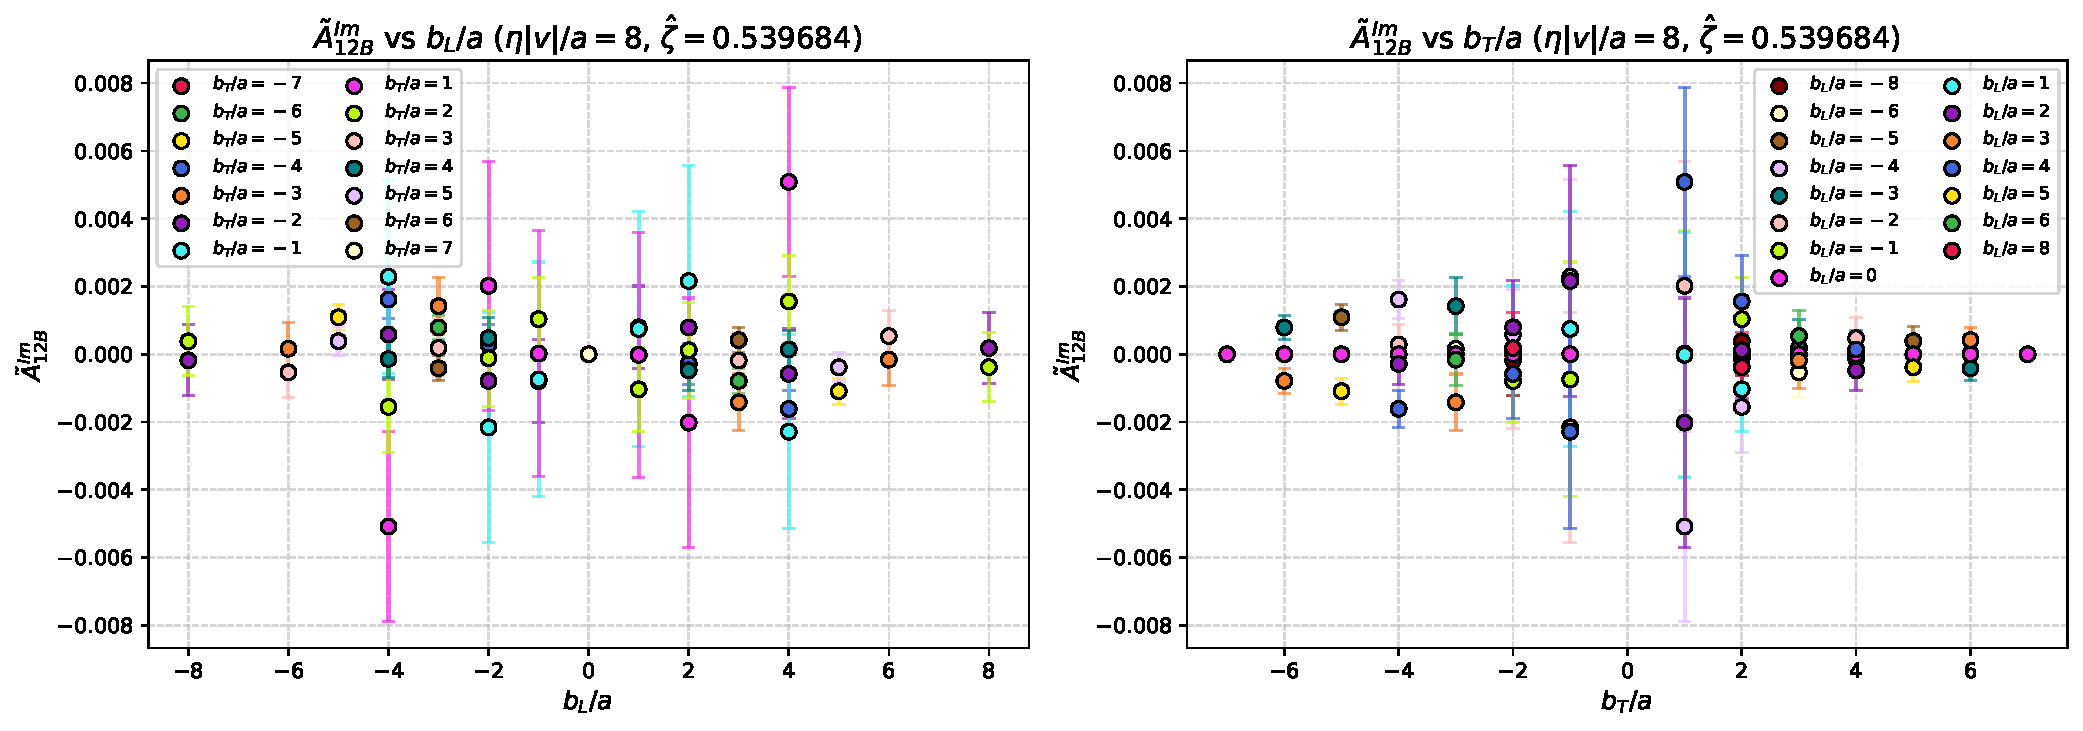
\includegraphics[width=0.98\linewidth,height=0.73\textheight,keepaspectratio]{ImA12B_eta8_PL-3_2D.pdf}\\[1mm]
{\small $\zetahat=0.539684$; $(b_L,b_T)$; $\eta|v|/a=8$ slices}
\figsrc{Thesis, Ch. 5: raw amplitude profiles; complete original panels.}
\end{frame}

\begin{frame}{$\tAmp_{12B}^{\mathrm{Im}}$ at $P_L=-3$: invariant coordinates}
\centering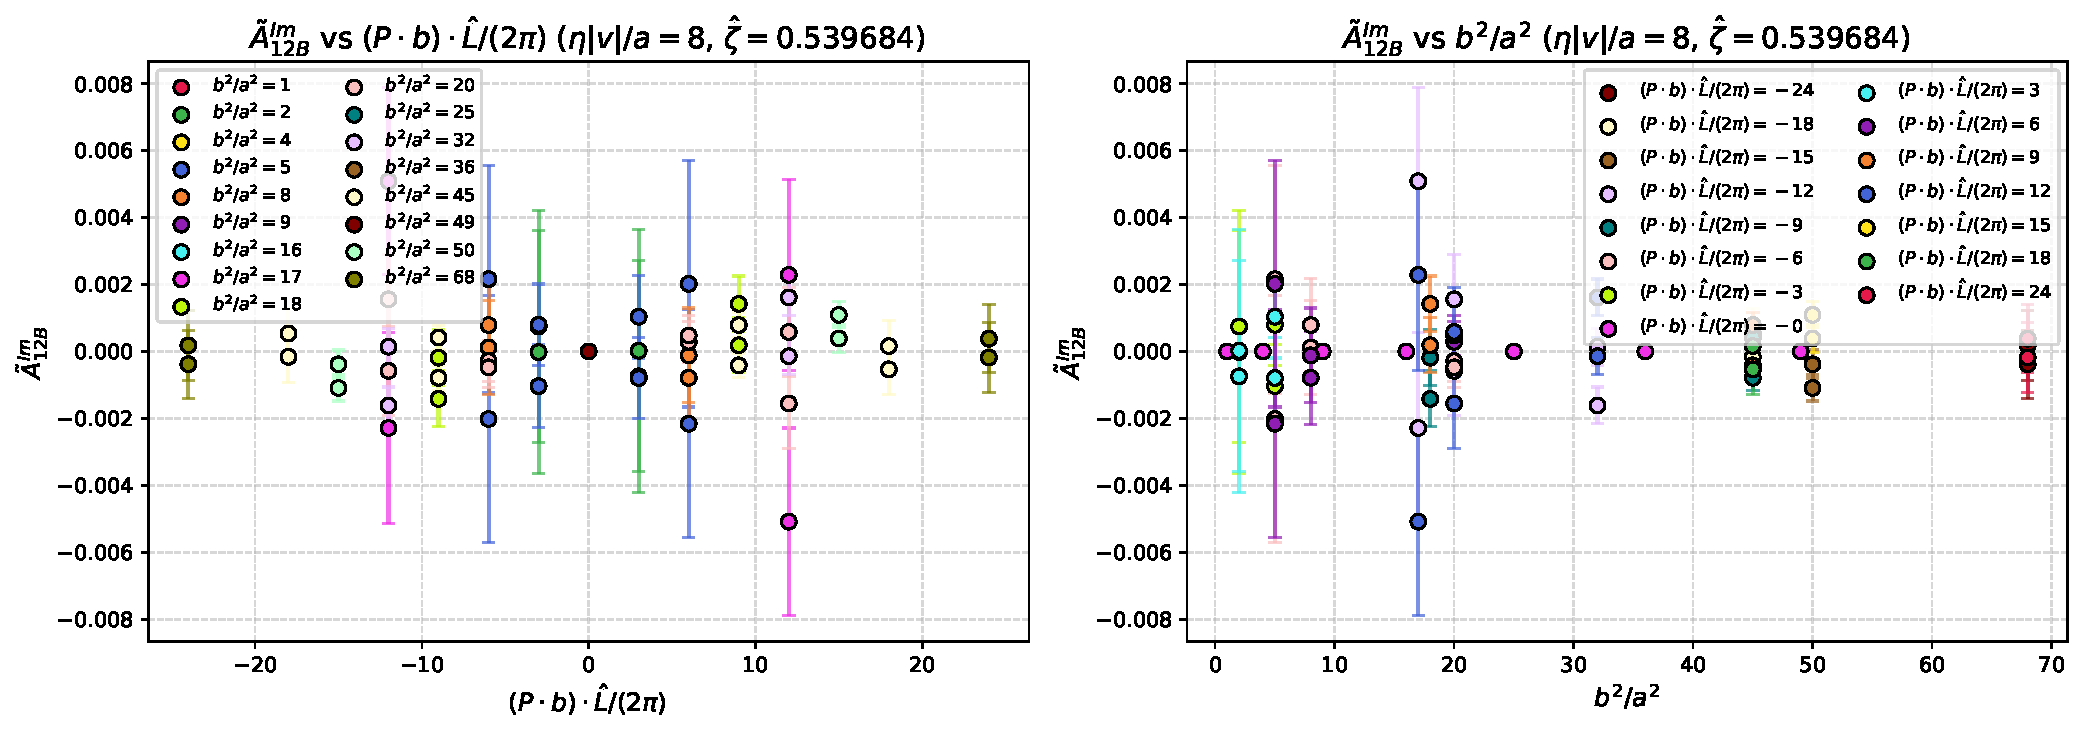
\includegraphics[width=0.98\linewidth,height=0.73\textheight,keepaspectratio]{ImA12B_Pb_bsq_eta8_PL-3_2D.pdf}\\[1mm]
{\small $\zetahat=0.539684$; $(\nu,s)$; $\eta|v|/a=8$ slices}
\figsrc{Thesis, Ch. 5: raw amplitude profiles; complete original panels.}
\end{frame}

\begin{frame}{$\tAmp_{2B}^{\mathrm{Re}}$ at $P_L=-4$: lattice coordinates}
\centering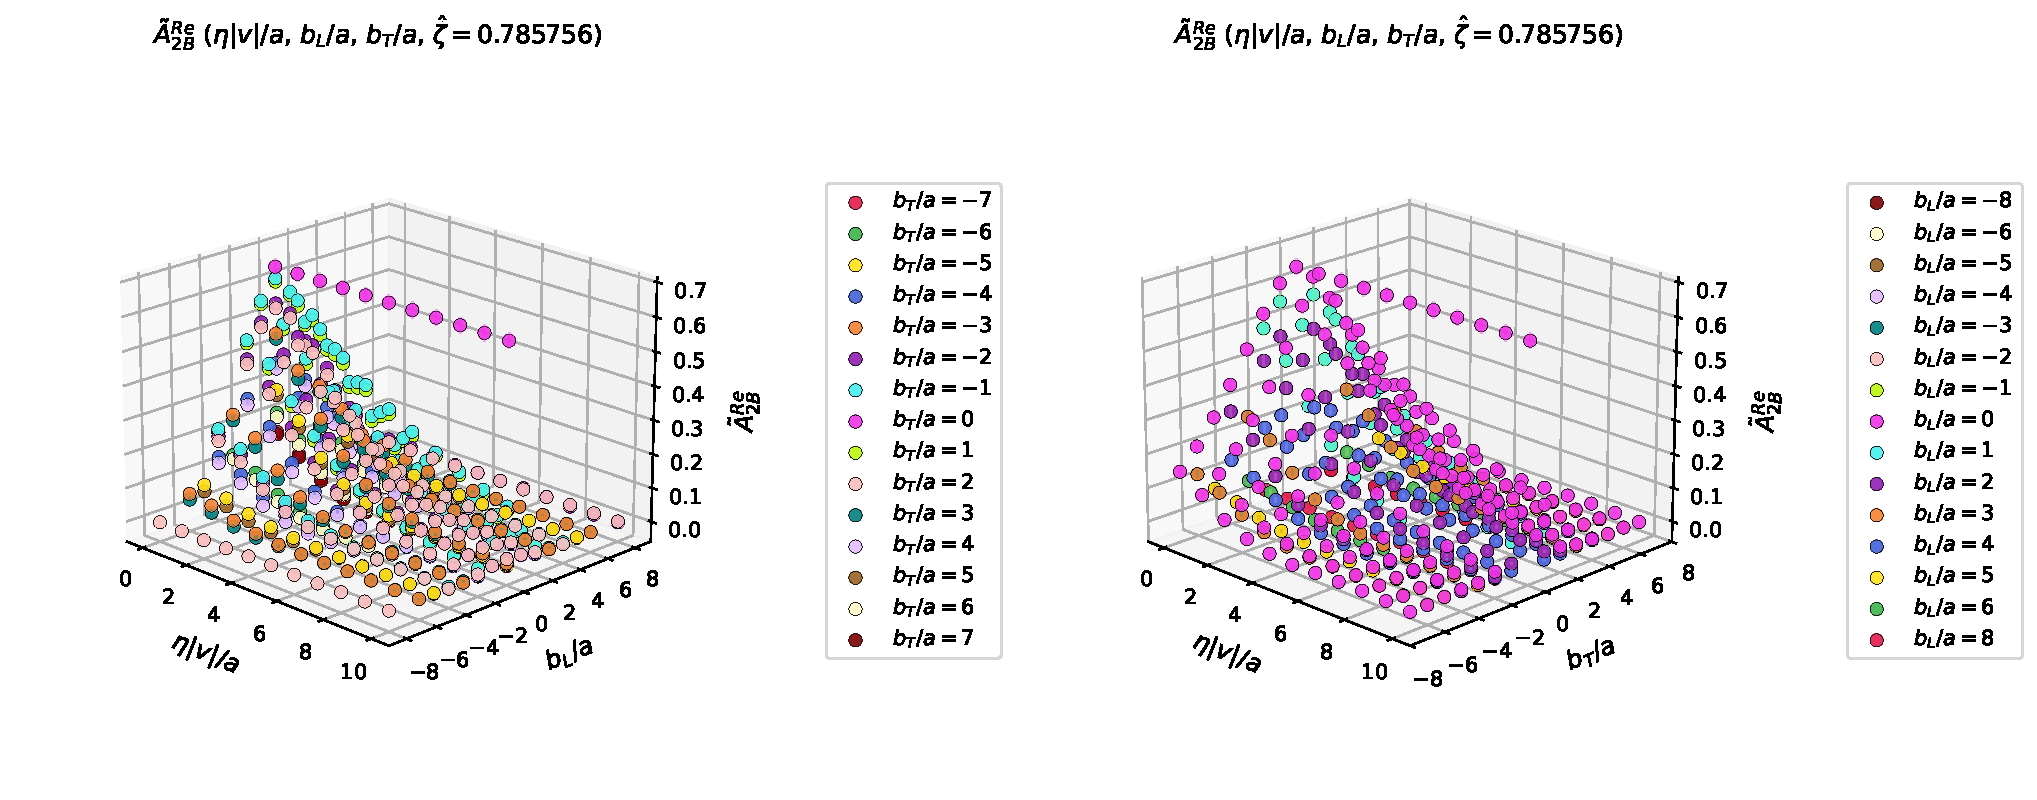
\includegraphics[width=0.98\linewidth,height=0.73\textheight,keepaspectratio]{ReA2B_PL-4_3D.pdf}\\[1mm]
{\small $\zetahat=0.785756$; $(b_L,b_T)$; staple-length dependence}
\figsrc{Thesis, Ch. 5: raw amplitude profiles; complete original panels.}
\end{frame}

\begin{frame}{$\tAmp_{2B}^{\mathrm{Re}}$ at $P_L=-4$: invariant coordinates}
\centering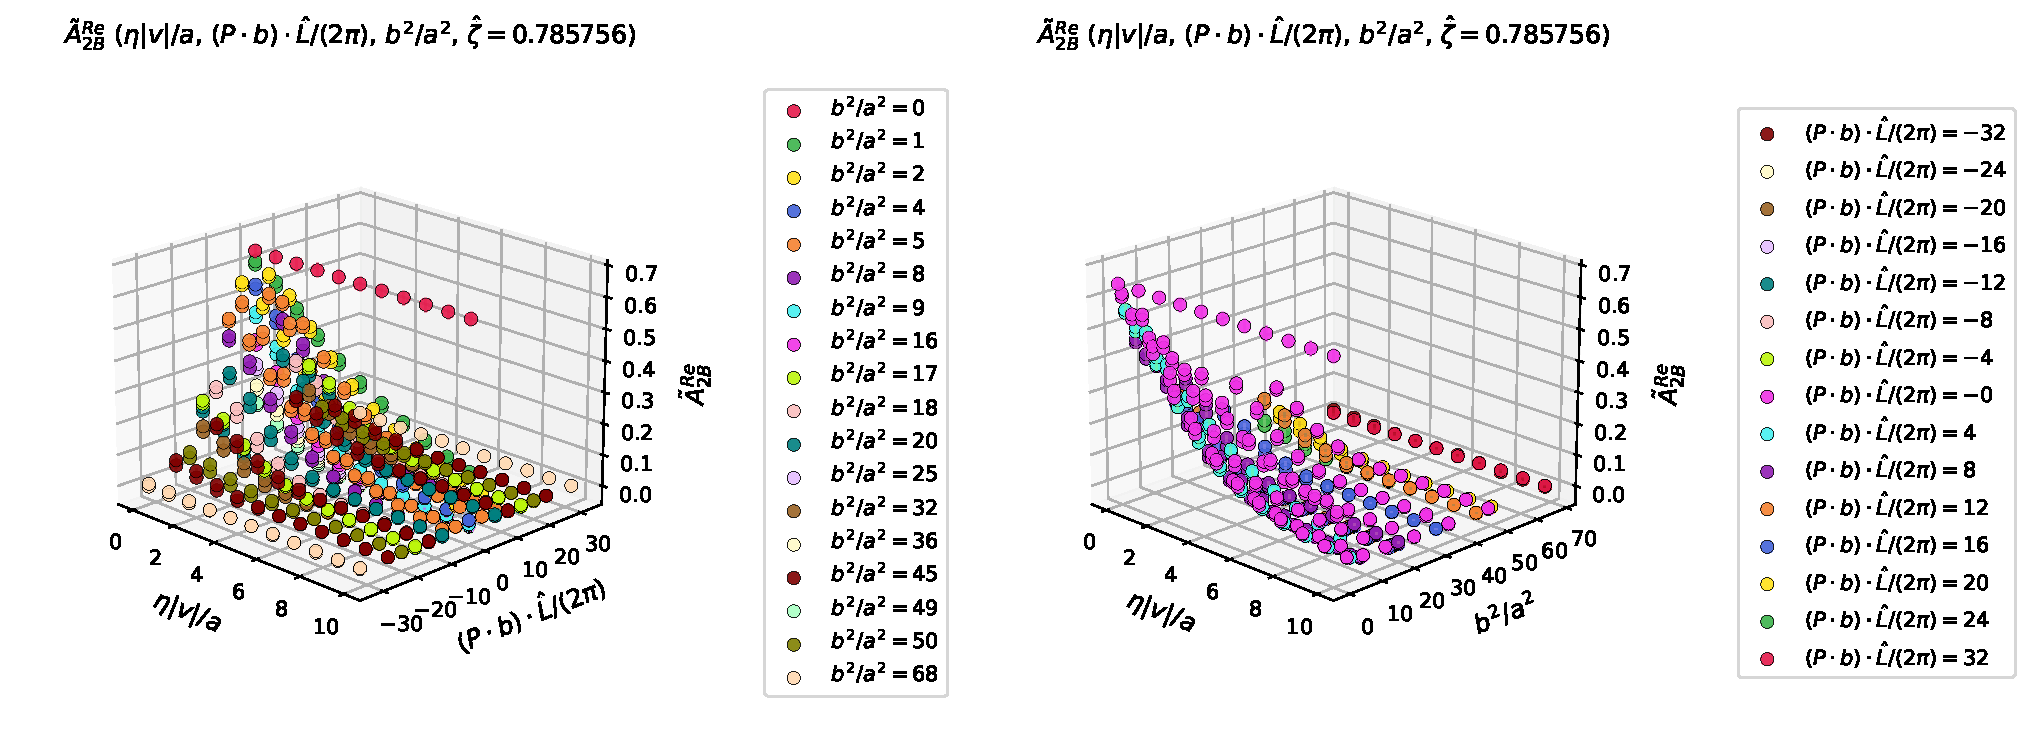
\includegraphics[width=0.98\linewidth,height=0.73\textheight,keepaspectratio]{ReA2B_Pb_bsq_PL-4_3D.pdf}\\[1mm]
{\small $\zetahat=0.785756$; $(\nu,s)$; staple-length dependence}
\figsrc{Thesis, Ch. 5: raw amplitude profiles; complete original panels.}
\end{frame}

\begin{frame}{$\tAmp_{2B}^{\mathrm{Im}}$ at $P_L=-4$: lattice coordinates}
\centering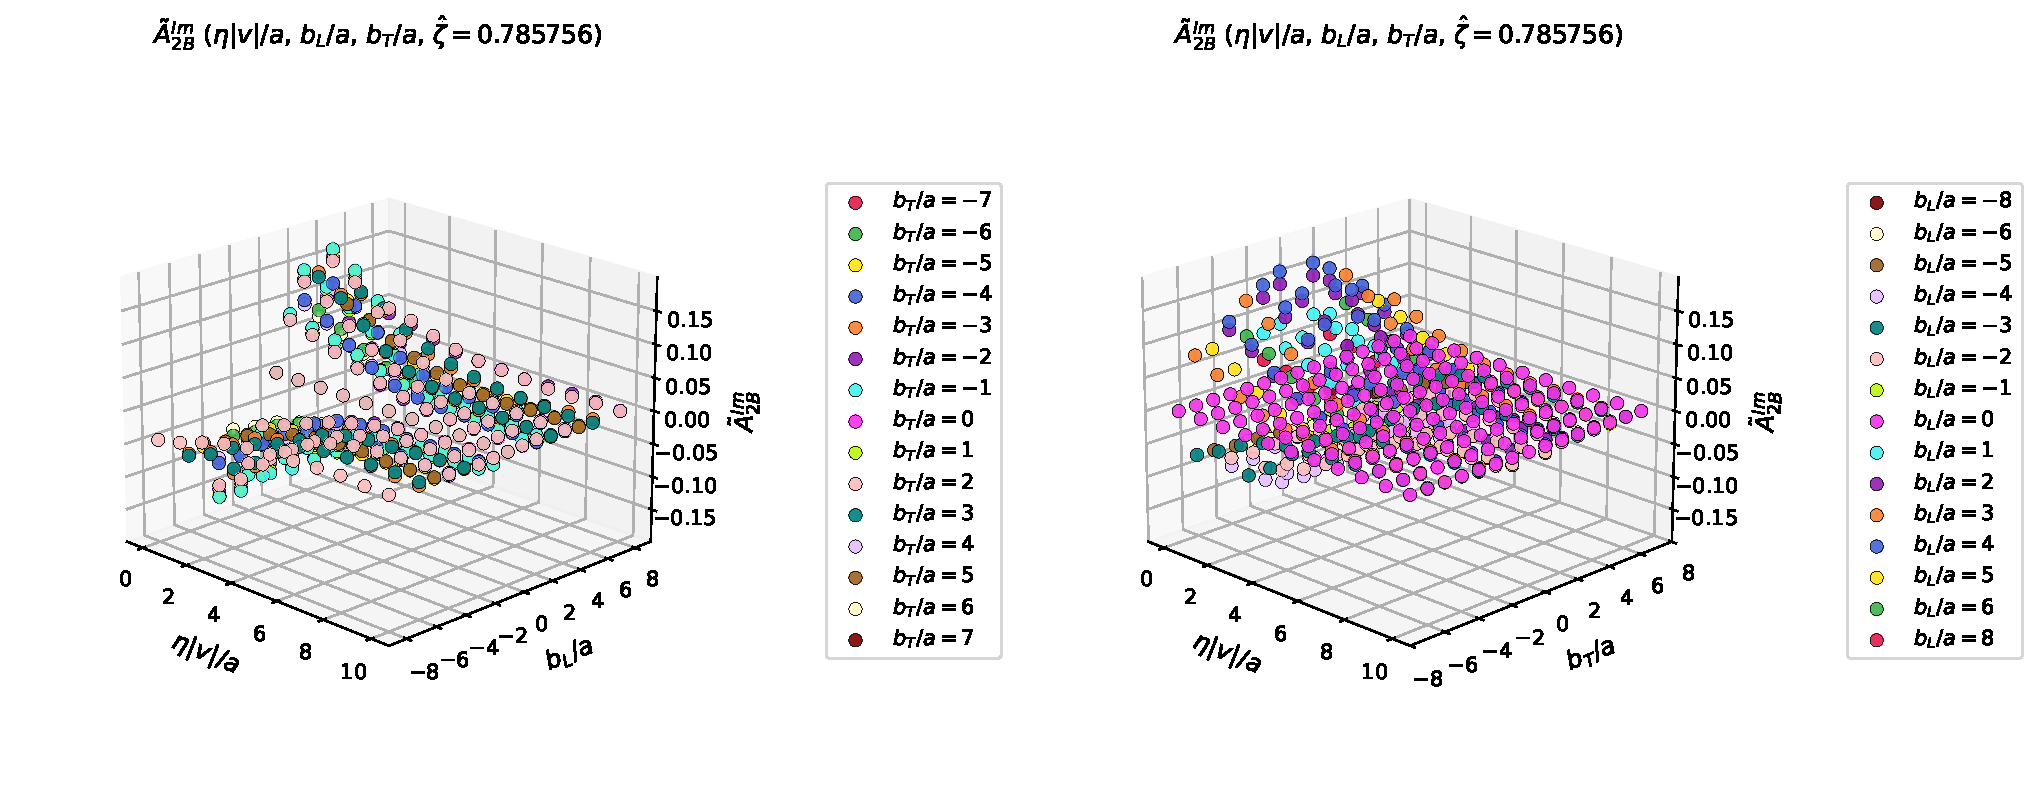
\includegraphics[width=0.98\linewidth,height=0.73\textheight,keepaspectratio]{ImA2B_PL-4_3D.pdf}\\[1mm]
{\small $\zetahat=0.785756$; $(b_L,b_T)$; staple-length dependence}
\figsrc{Thesis, Ch. 5: raw amplitude profiles; complete original panels.}
\end{frame}

\begin{frame}{$\tAmp_{2B}^{\mathrm{Im}}$ at $P_L=-4$: invariant coordinates}
\centering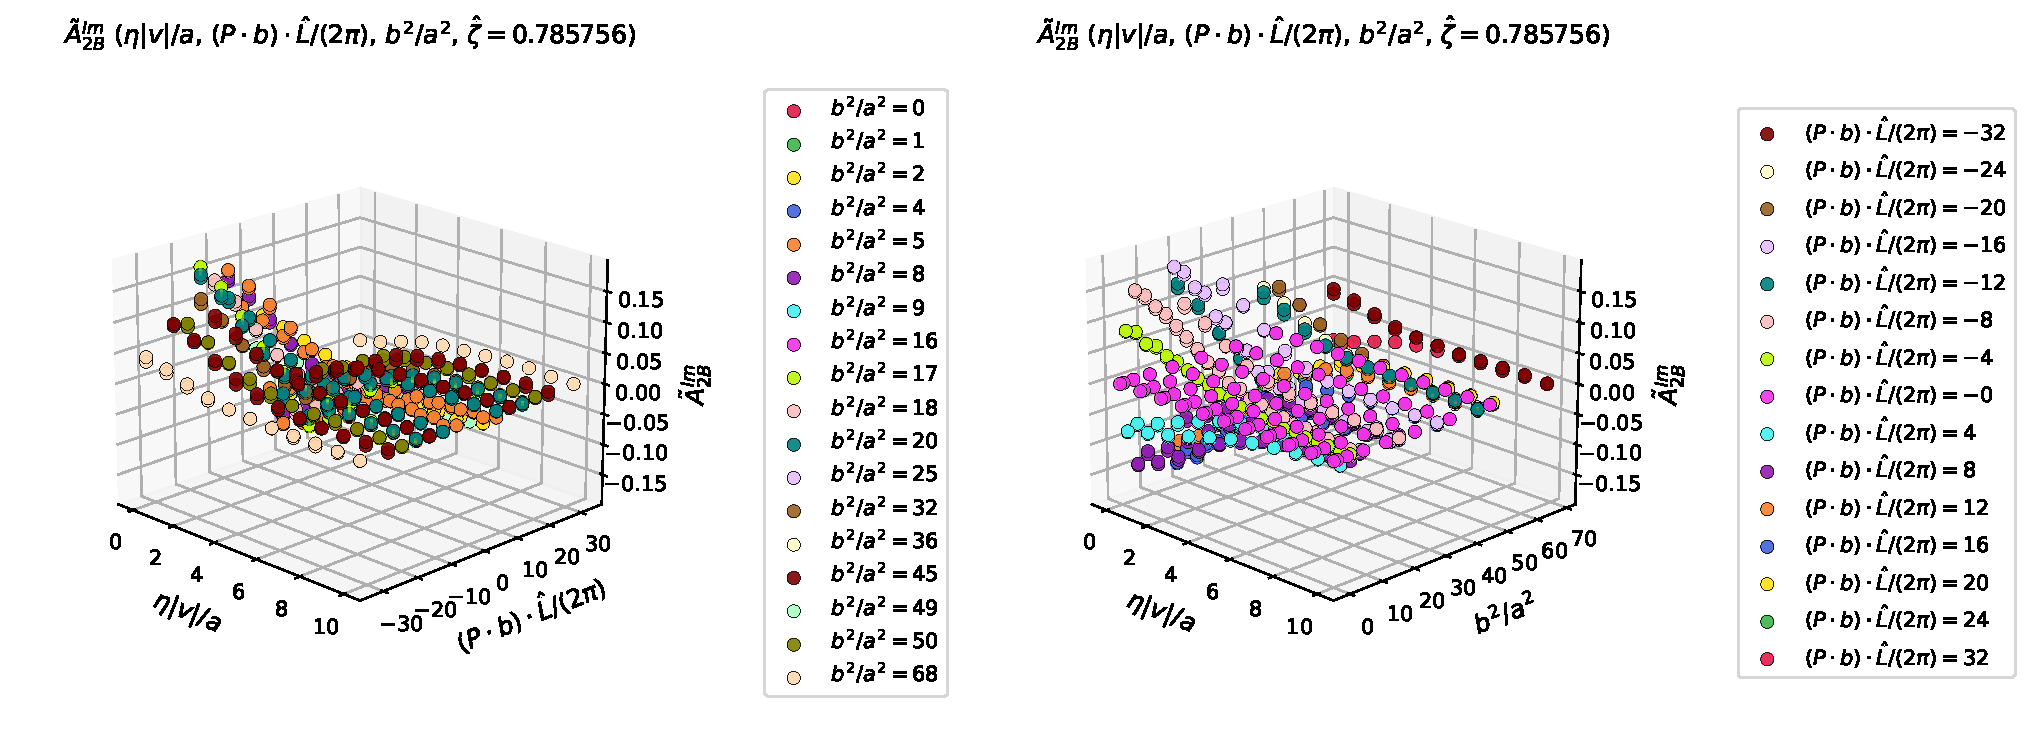
\includegraphics[width=0.98\linewidth,height=0.73\textheight,keepaspectratio]{ImA2B_Pb_bsq_PL-4_3D.pdf}\\[1mm]
{\small $\zetahat=0.785756$; $(\nu,s)$; staple-length dependence}
\figsrc{Thesis, Ch. 5: raw amplitude profiles; complete original panels.}
\end{frame}

\begin{frame}{$\tAmp_{12B}^{\mathrm{Re}}$ at $P_L=-4$: lattice coordinates}
\centering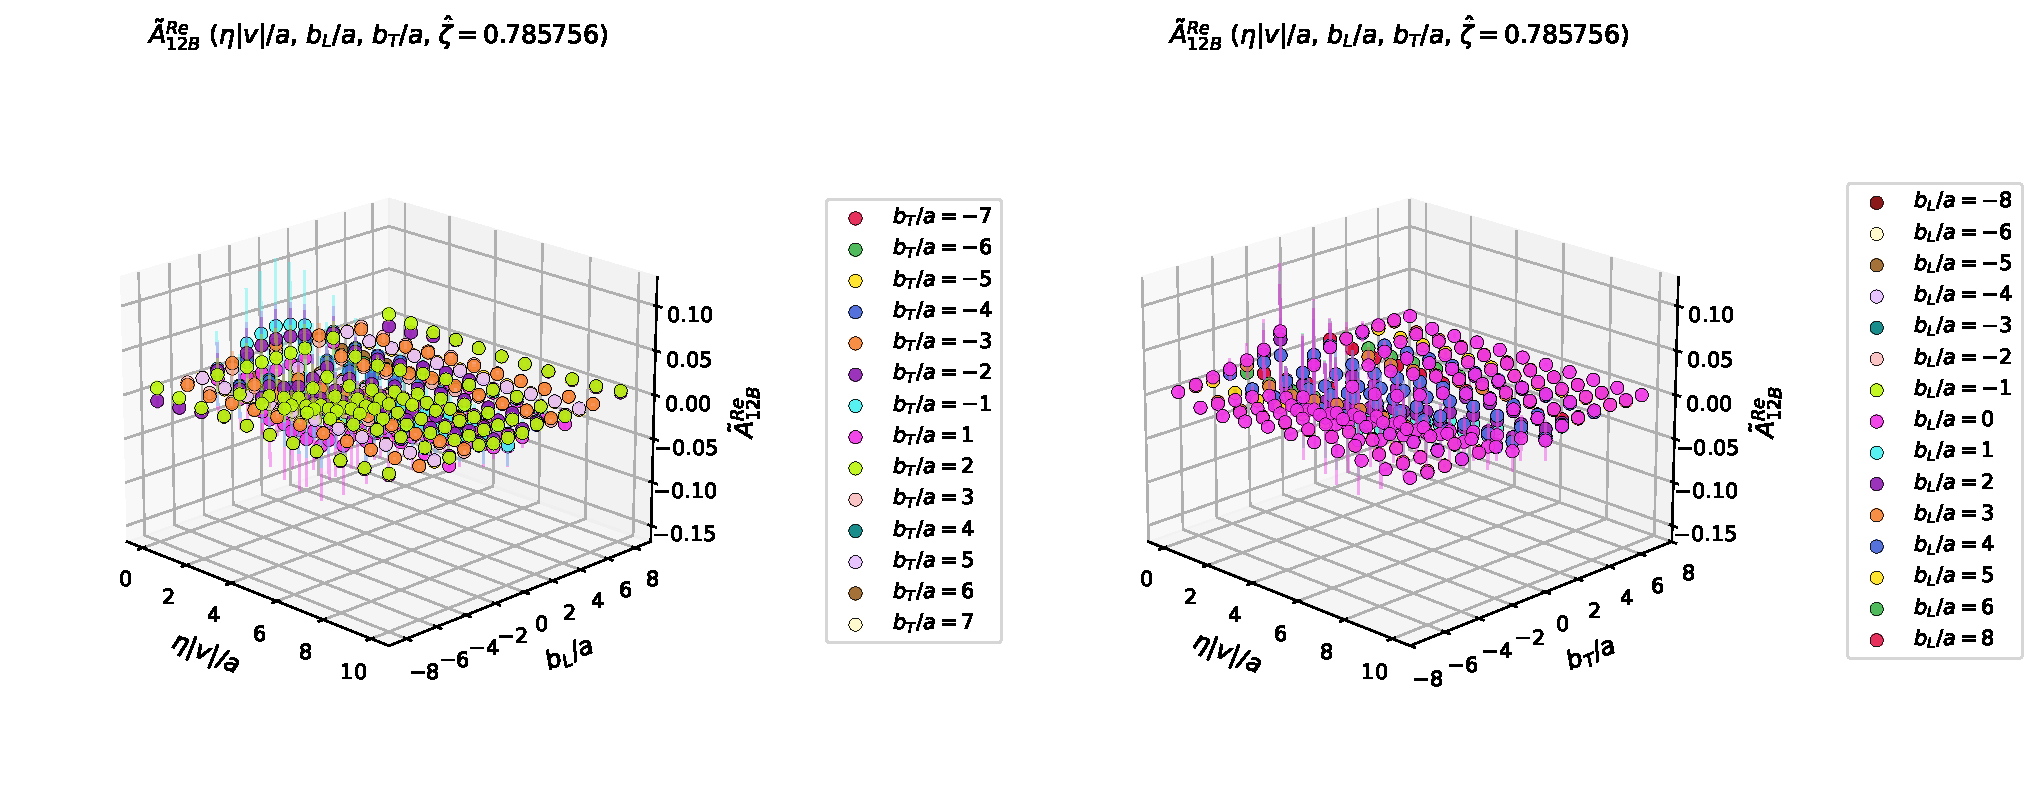
\includegraphics[width=0.98\linewidth,height=0.73\textheight,keepaspectratio]{ReA12B_PL-4_3D.pdf}\\[1mm]
{\small $\zetahat=0.785756$; $(b_L,b_T)$; staple-length dependence}
\figsrc{Thesis, Ch. 5: raw amplitude profiles; complete original panels.}
\end{frame}

\begin{frame}{$\tAmp_{12B}^{\mathrm{Re}}$ at $P_L=-4$: invariant coordinates}
\centering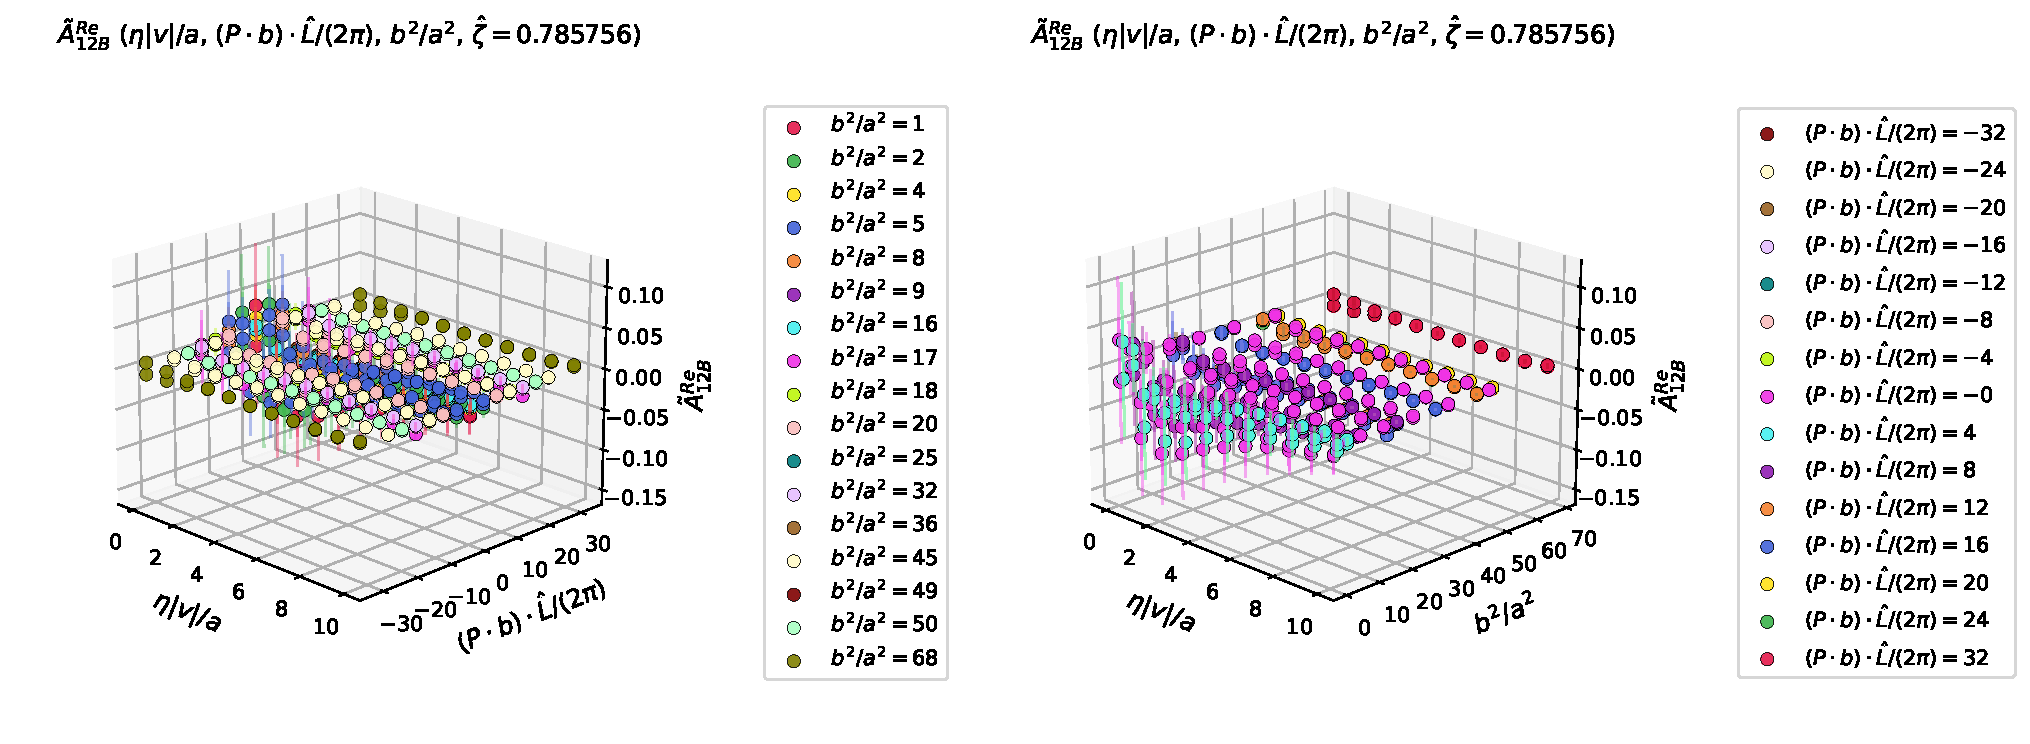
\includegraphics[width=0.98\linewidth,height=0.73\textheight,keepaspectratio]{ReA12B_Pb_bsq_PL-4_3D.pdf}\\[1mm]
{\small $\zetahat=0.785756$; $(\nu,s)$; staple-length dependence}
\figsrc{Thesis, Ch. 5: raw amplitude profiles; complete original panels.}
\end{frame}

\begin{frame}{$\tAmp_{12B}^{\mathrm{Im}}$ at $P_L=-4$: lattice coordinates}
\centering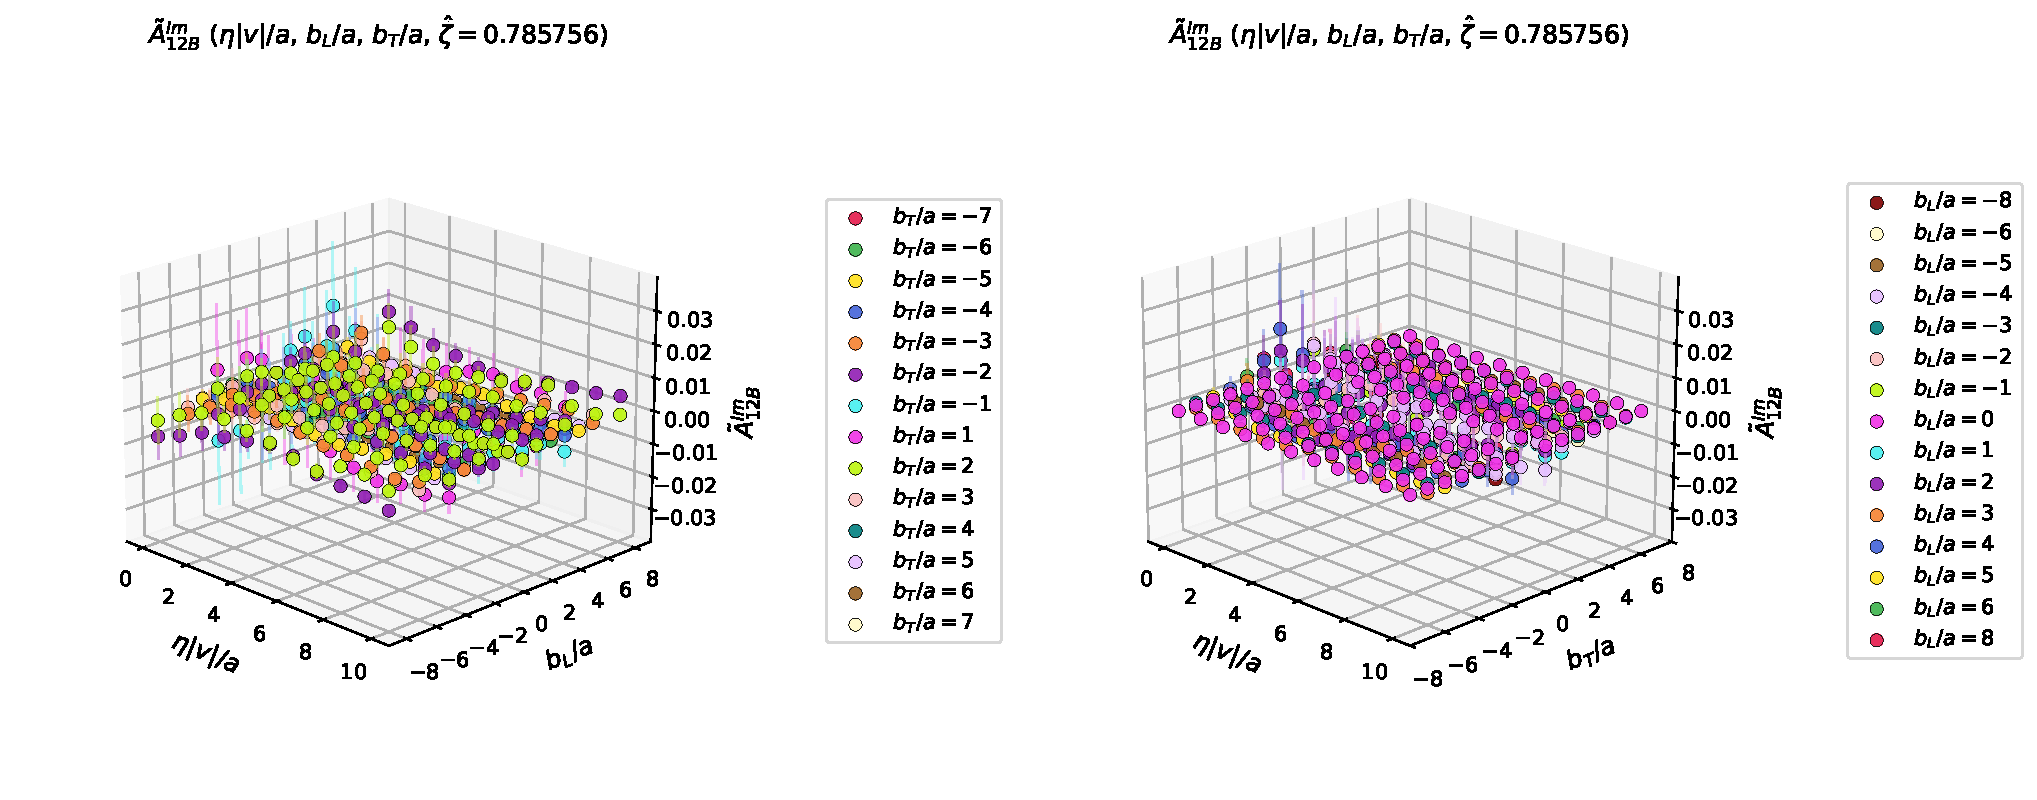
\includegraphics[width=0.98\linewidth,height=0.73\textheight,keepaspectratio]{ImA12B_PL-4_3D.pdf}\\[1mm]
{\small $\zetahat=0.785756$; $(b_L,b_T)$; staple-length dependence}
\figsrc{Thesis, Ch. 5: raw amplitude profiles; complete original panels.}
\end{frame}

\begin{frame}{$\tAmp_{12B}^{\mathrm{Im}}$ at $P_L=-4$: invariant coordinates}
\centering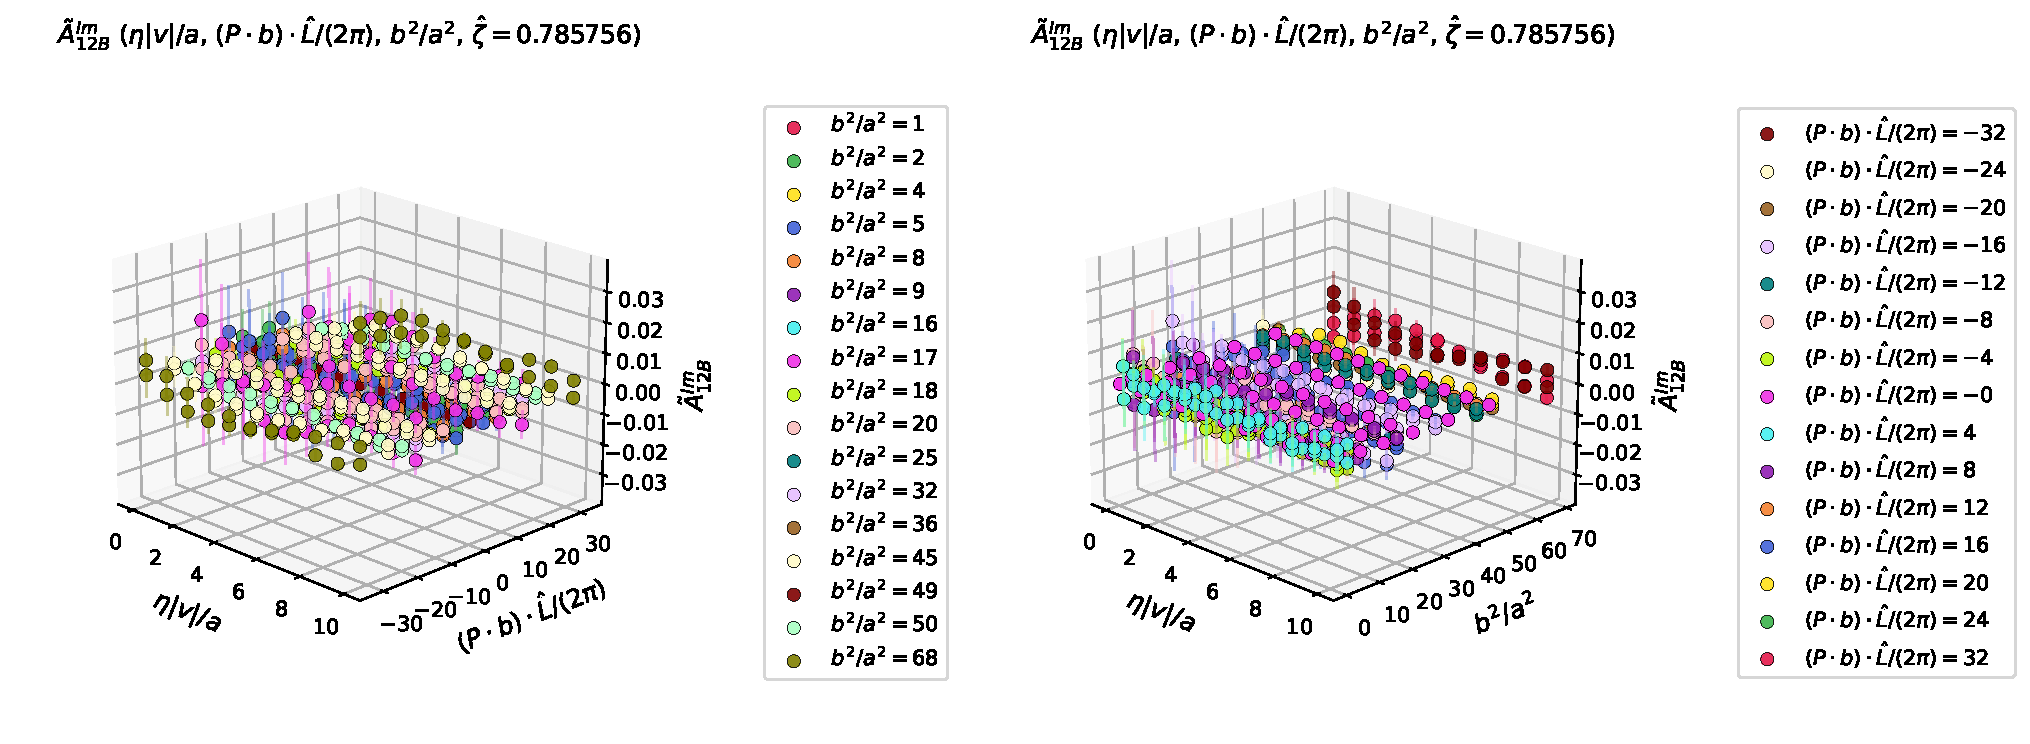
\includegraphics[width=0.98\linewidth,height=0.73\textheight,keepaspectratio]{ImA12B_Pb_bsq_PL-4_3D.pdf}\\[1mm]
{\small $\zetahat=0.785756$; $(\nu,s)$; staple-length dependence}
\figsrc{Thesis, Ch. 5: raw amplitude profiles; complete original panels.}
\end{frame}

\begin{frame}{$\tAmp_{2B}^{\mathrm{Re}}$ at $P_L=-4$: lattice coordinates}
\centering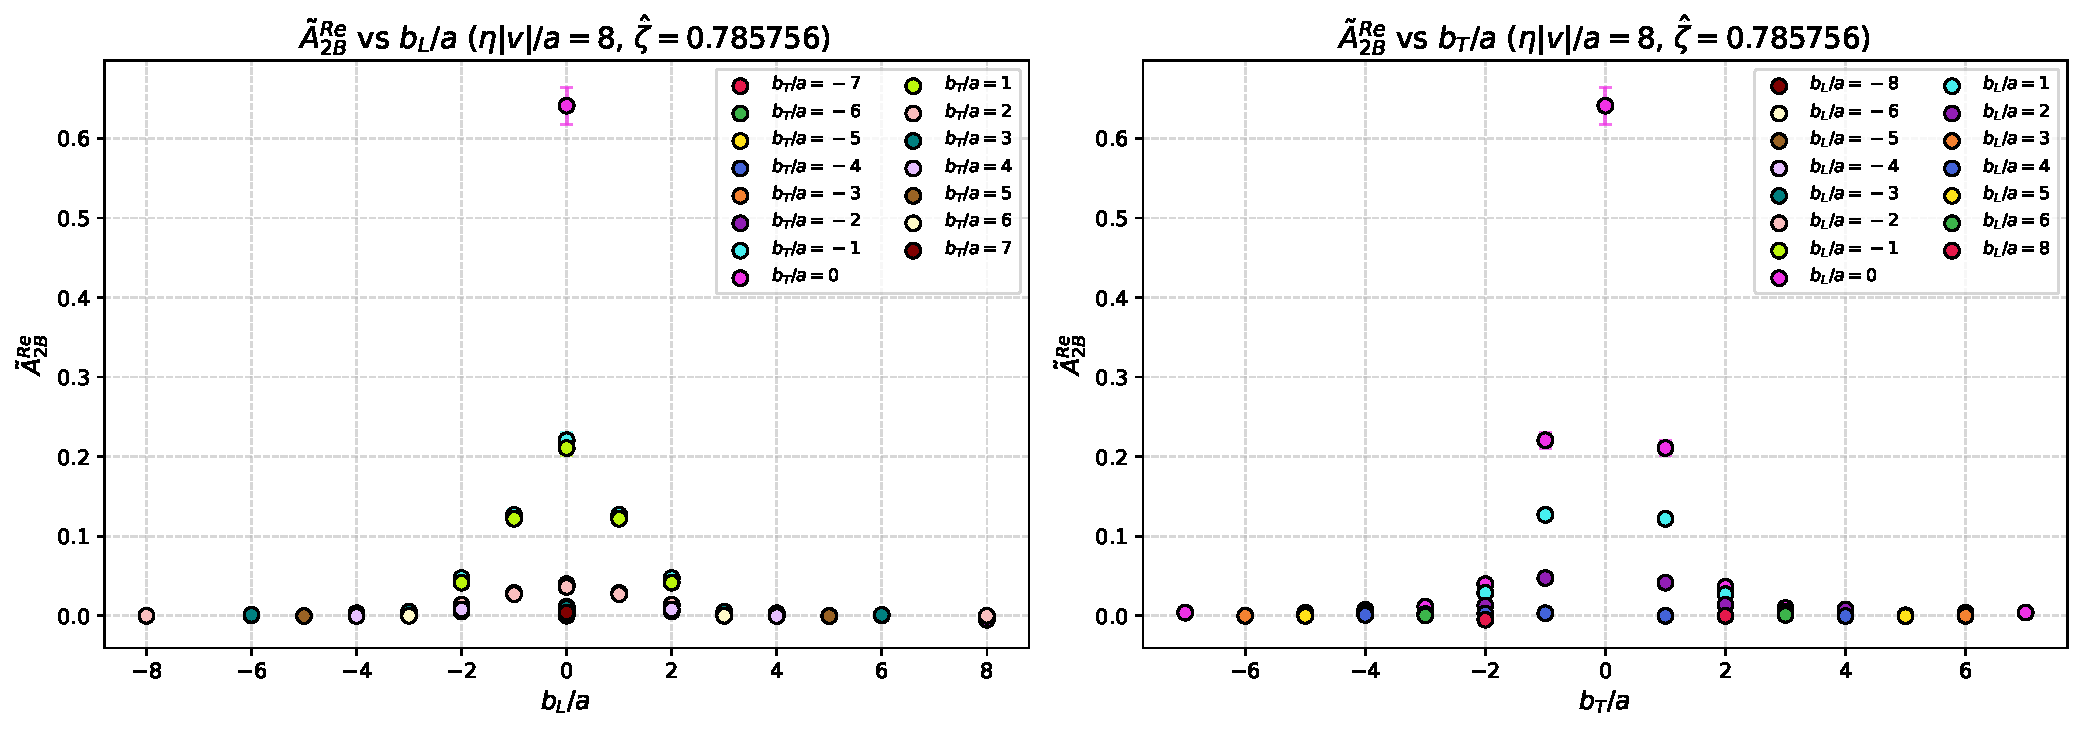
\includegraphics[width=0.98\linewidth,height=0.73\textheight,keepaspectratio]{ReA2B_eta8_PL-4_2D.pdf}\\[1mm]
{\small $\zetahat=0.785756$; $(b_L,b_T)$; $\eta|v|/a=8$ slices}
\figsrc{Thesis, Ch. 5: raw amplitude profiles; complete original panels.}
\end{frame}

\begin{frame}{$\tAmp_{2B}^{\mathrm{Re}}$ at $P_L=-4$: invariant coordinates}
\centering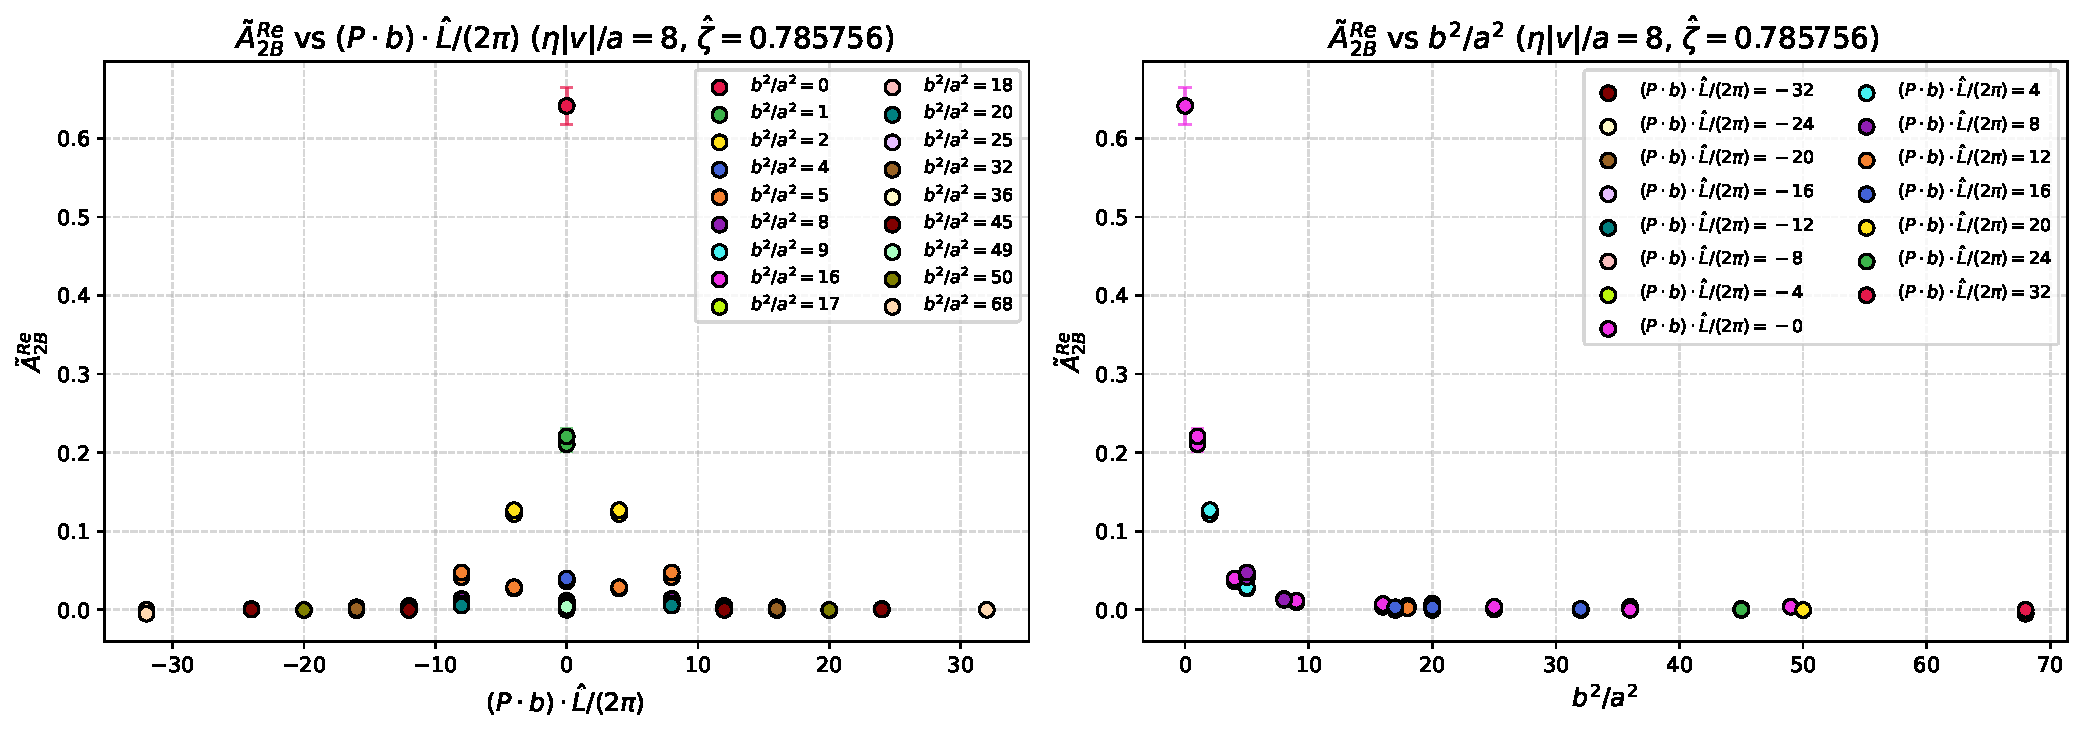
\includegraphics[width=0.98\linewidth,height=0.73\textheight,keepaspectratio]{ReA2B_Pb_bsq_eta8_PL-4_2D.pdf}\\[1mm]
{\small $\zetahat=0.785756$; $(\nu,s)$; $\eta|v|/a=8$ slices}
\figsrc{Thesis, Ch. 5: raw amplitude profiles; complete original panels.}
\end{frame}

\begin{frame}{$\tAmp_{2B}^{\mathrm{Im}}$ at $P_L=-4$: lattice coordinates}
\centering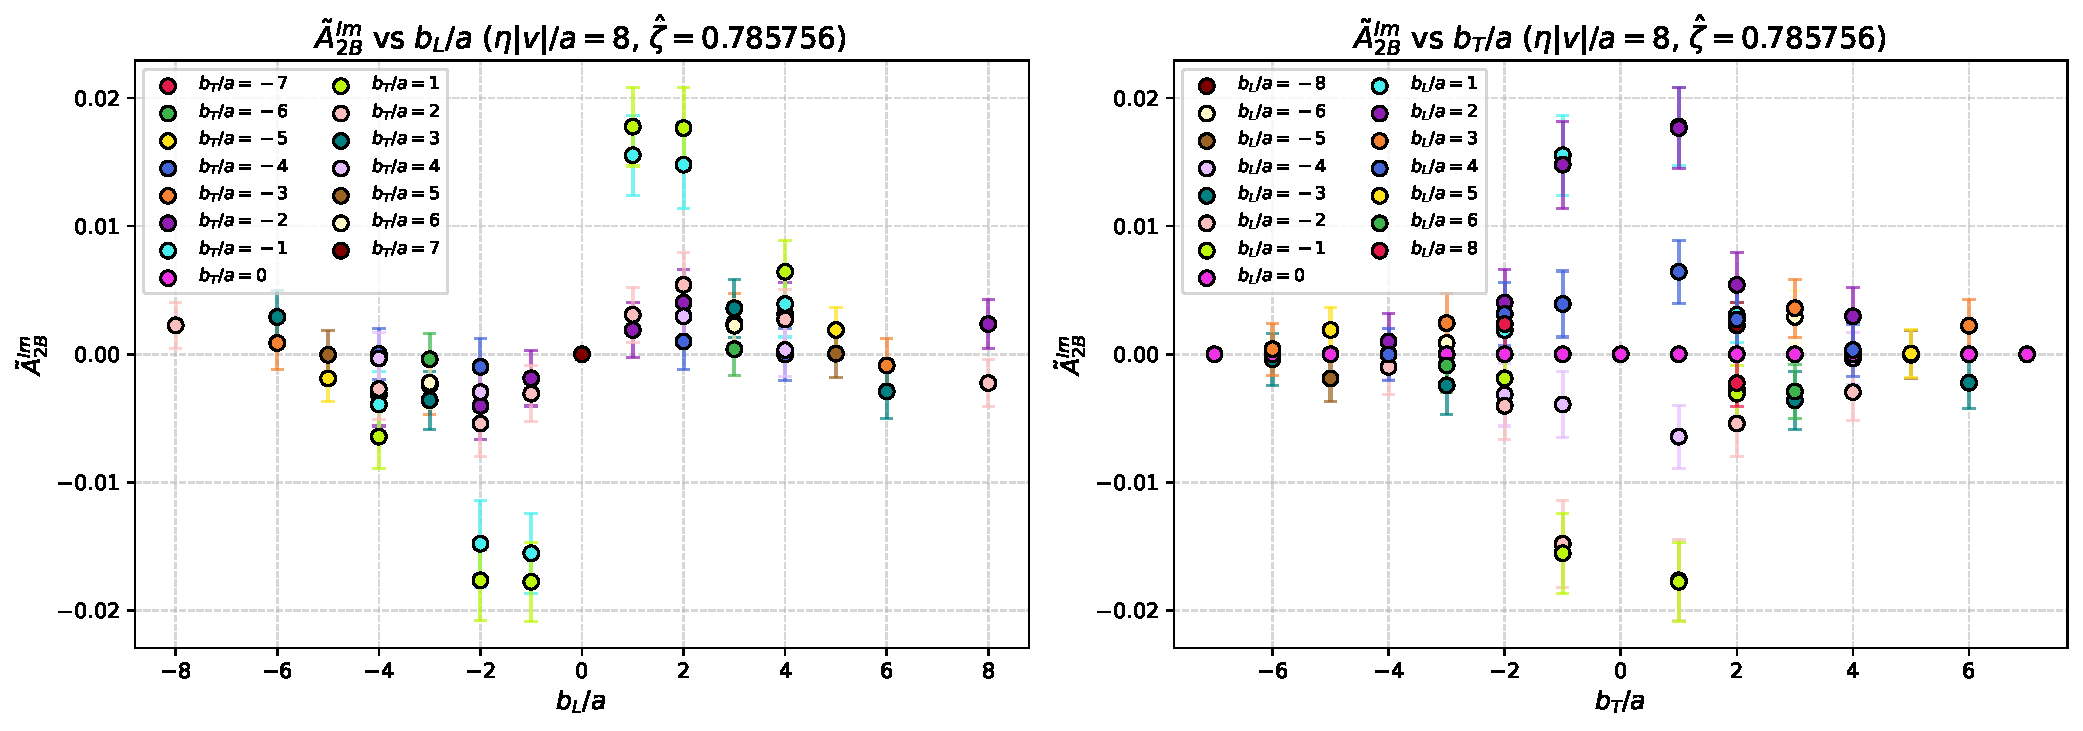
\includegraphics[width=0.98\linewidth,height=0.73\textheight,keepaspectratio]{ImA2B_eta8_PL-4_2D.pdf}\\[1mm]
{\small $\zetahat=0.785756$; $(b_L,b_T)$; $\eta|v|/a=8$ slices}
\figsrc{Thesis, Ch. 5: raw amplitude profiles; complete original panels.}
\end{frame}

\begin{frame}{$\tAmp_{2B}^{\mathrm{Im}}$ at $P_L=-4$: invariant coordinates}
\centering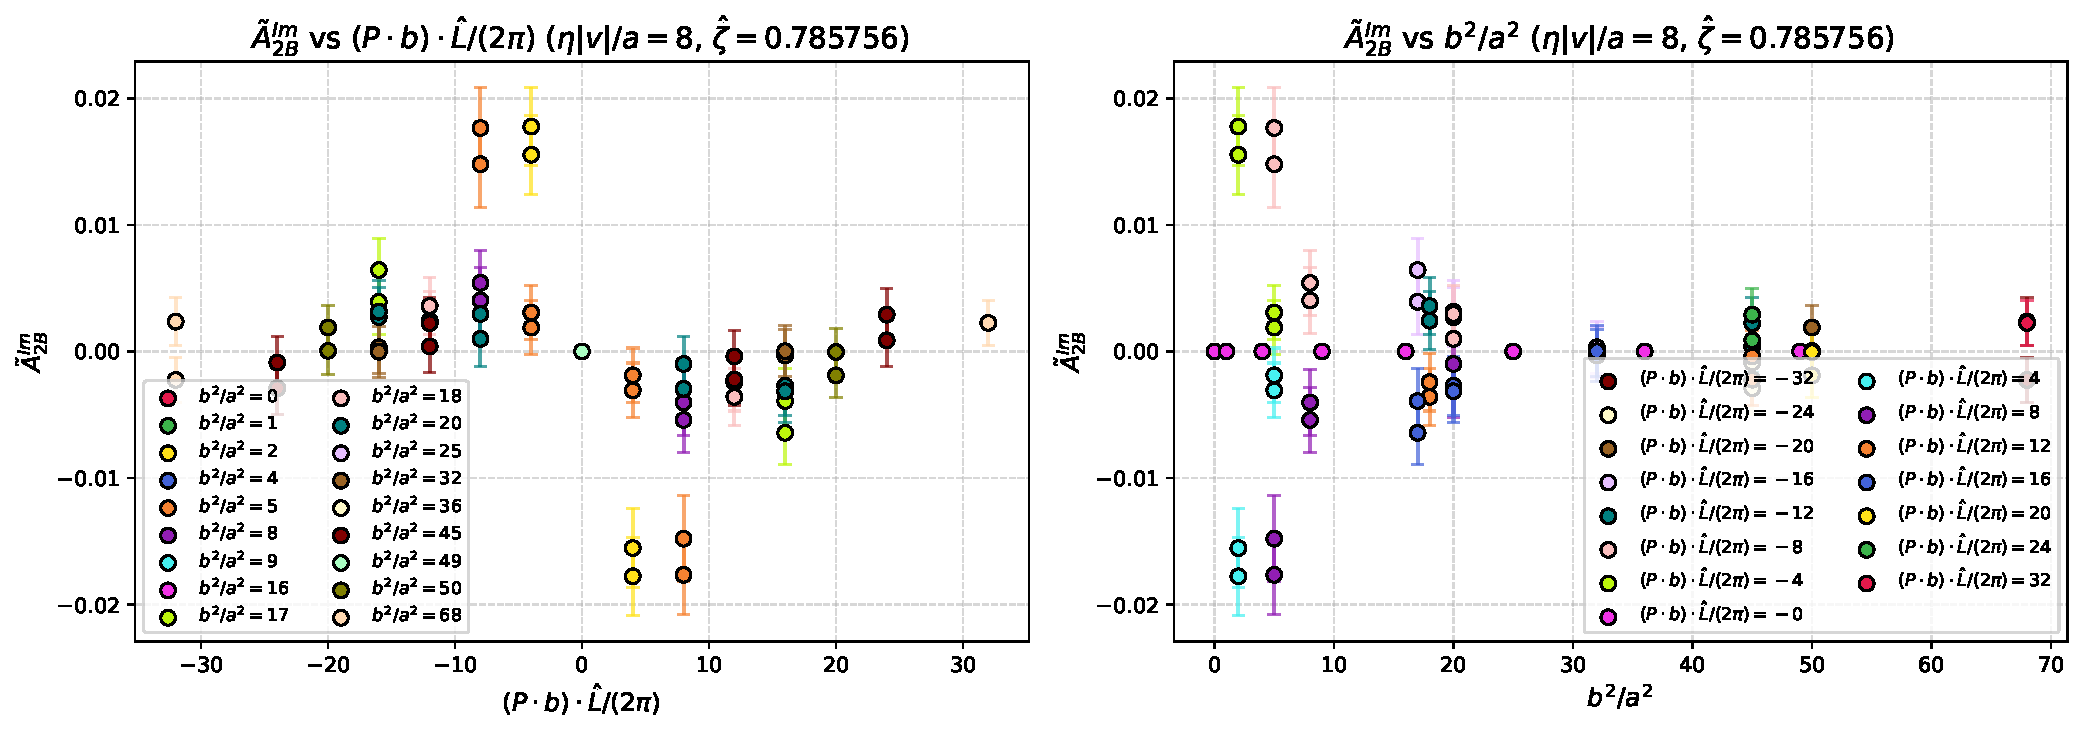
\includegraphics[width=0.98\linewidth,height=0.73\textheight,keepaspectratio]{ImA2B_Pb_bsq_eta8_PL-4_2D.pdf}\\[1mm]
{\small $\zetahat=0.785756$; $(\nu,s)$; $\eta|v|/a=8$ slices}
\figsrc{Thesis, Ch. 5: raw amplitude profiles; complete original panels.}
\end{frame}

\begin{frame}{$\tAmp_{12B}^{\mathrm{Re}}$ at $P_L=-4$: lattice coordinates}
\centering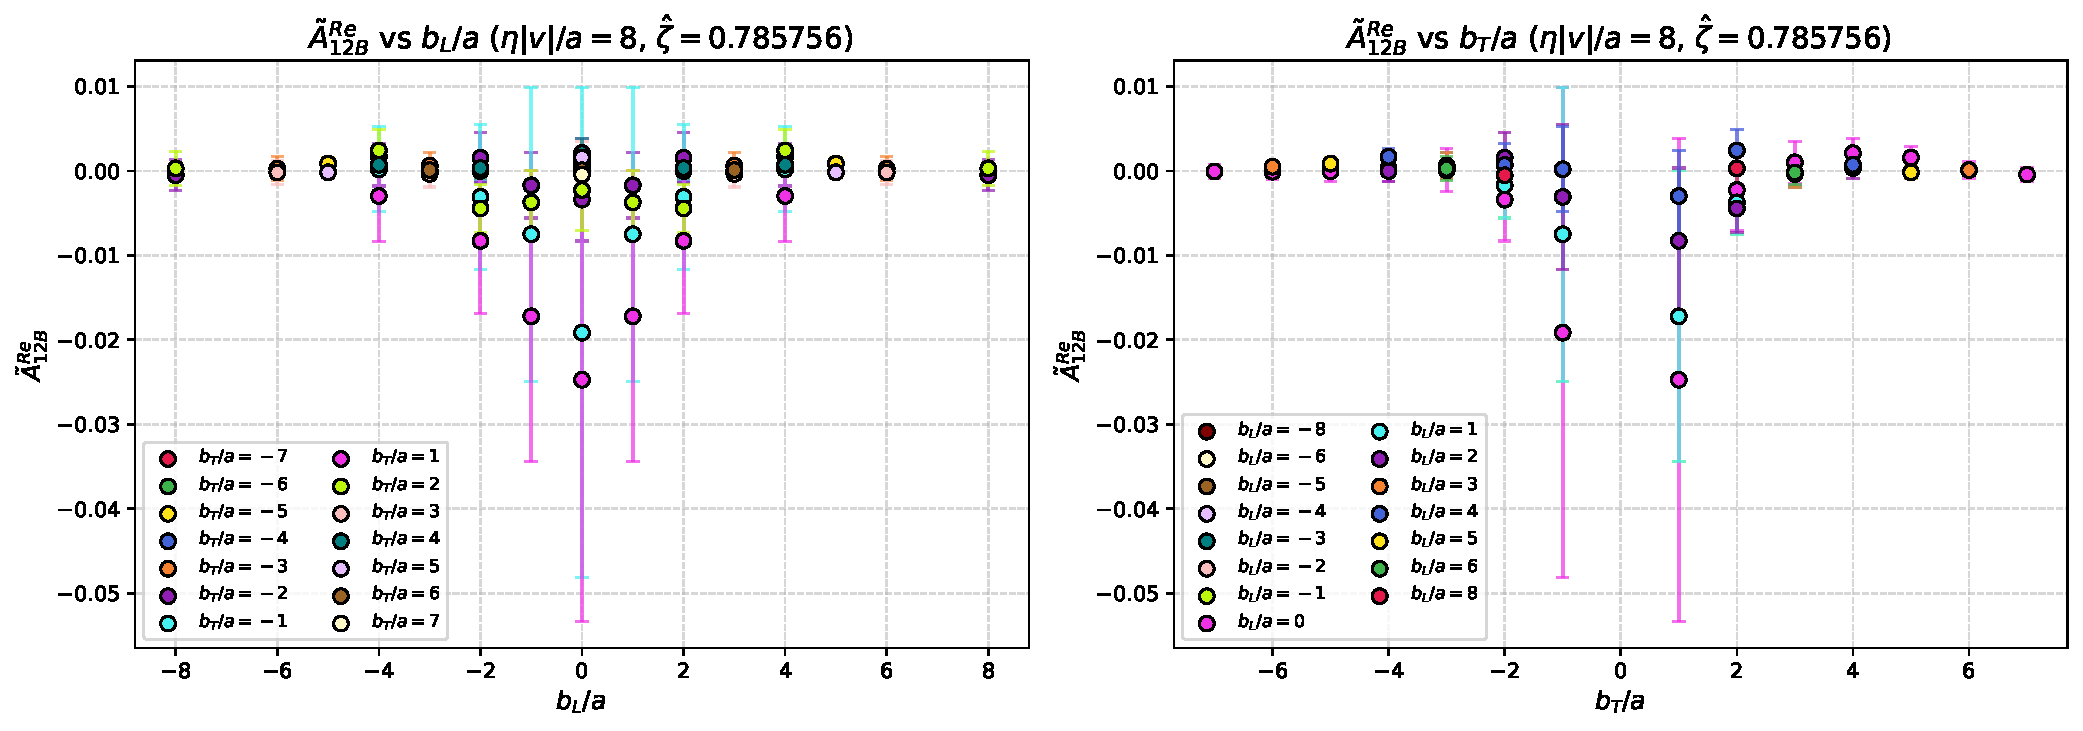
\includegraphics[width=0.98\linewidth,height=0.73\textheight,keepaspectratio]{ReA12B_eta8_PL-4_2D.pdf}\\[1mm]
{\small $\zetahat=0.785756$; $(b_L,b_T)$; $\eta|v|/a=8$ slices}
\figsrc{Thesis, Ch. 5: raw amplitude profiles; complete original panels.}
\end{frame}

\begin{frame}{$\tAmp_{12B}^{\mathrm{Re}}$ at $P_L=-4$: invariant coordinates}
\centering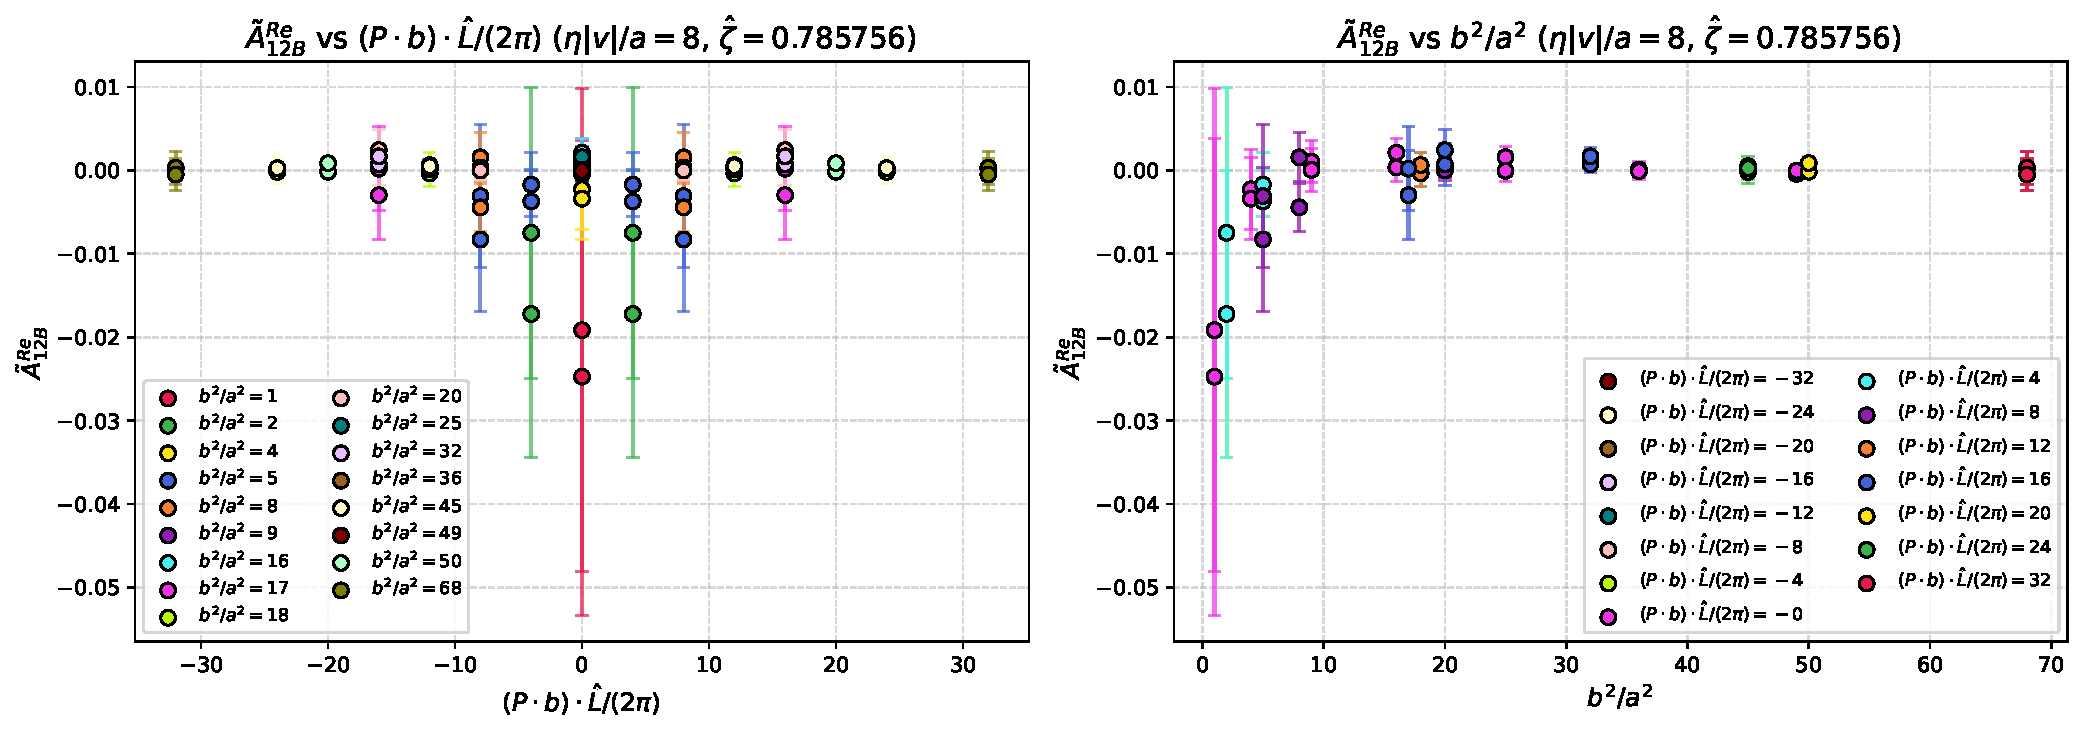
\includegraphics[width=0.98\linewidth,height=0.73\textheight,keepaspectratio]{ReA12B_Pb_bsq_eta8_PL-4_2D.pdf}\\[1mm]
{\small $\zetahat=0.785756$; $(\nu,s)$; $\eta|v|/a=8$ slices}
\figsrc{Thesis, Ch. 5: raw amplitude profiles; complete original panels.}
\end{frame}

\begin{frame}{$\tAmp_{12B}^{\mathrm{Im}}$ at $P_L=-4$: lattice coordinates}
\centering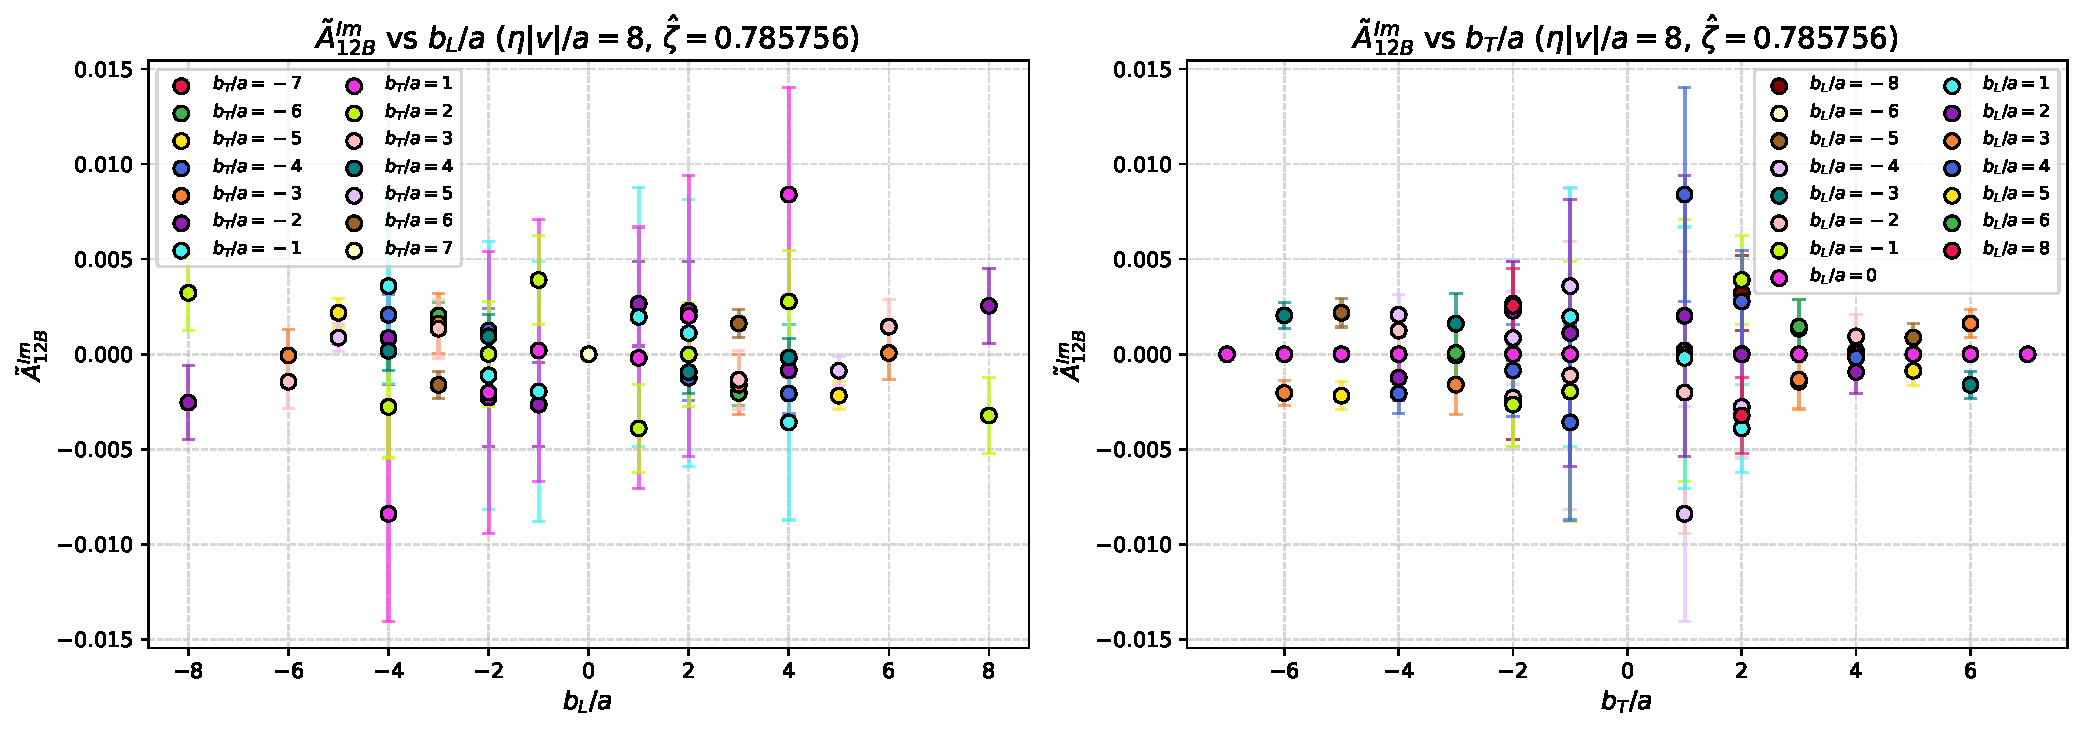
\includegraphics[width=0.98\linewidth,height=0.73\textheight,keepaspectratio]{ImA12B_eta8_PL-4_2D.pdf}\\[1mm]
{\small $\zetahat=0.785756$; $(b_L,b_T)$; $\eta|v|/a=8$ slices}
\figsrc{Thesis, Ch. 5: raw amplitude profiles; complete original panels.}
\end{frame}

\begin{frame}{$\tAmp_{12B}^{\mathrm{Im}}$ at $P_L=-4$: invariant coordinates}
\centering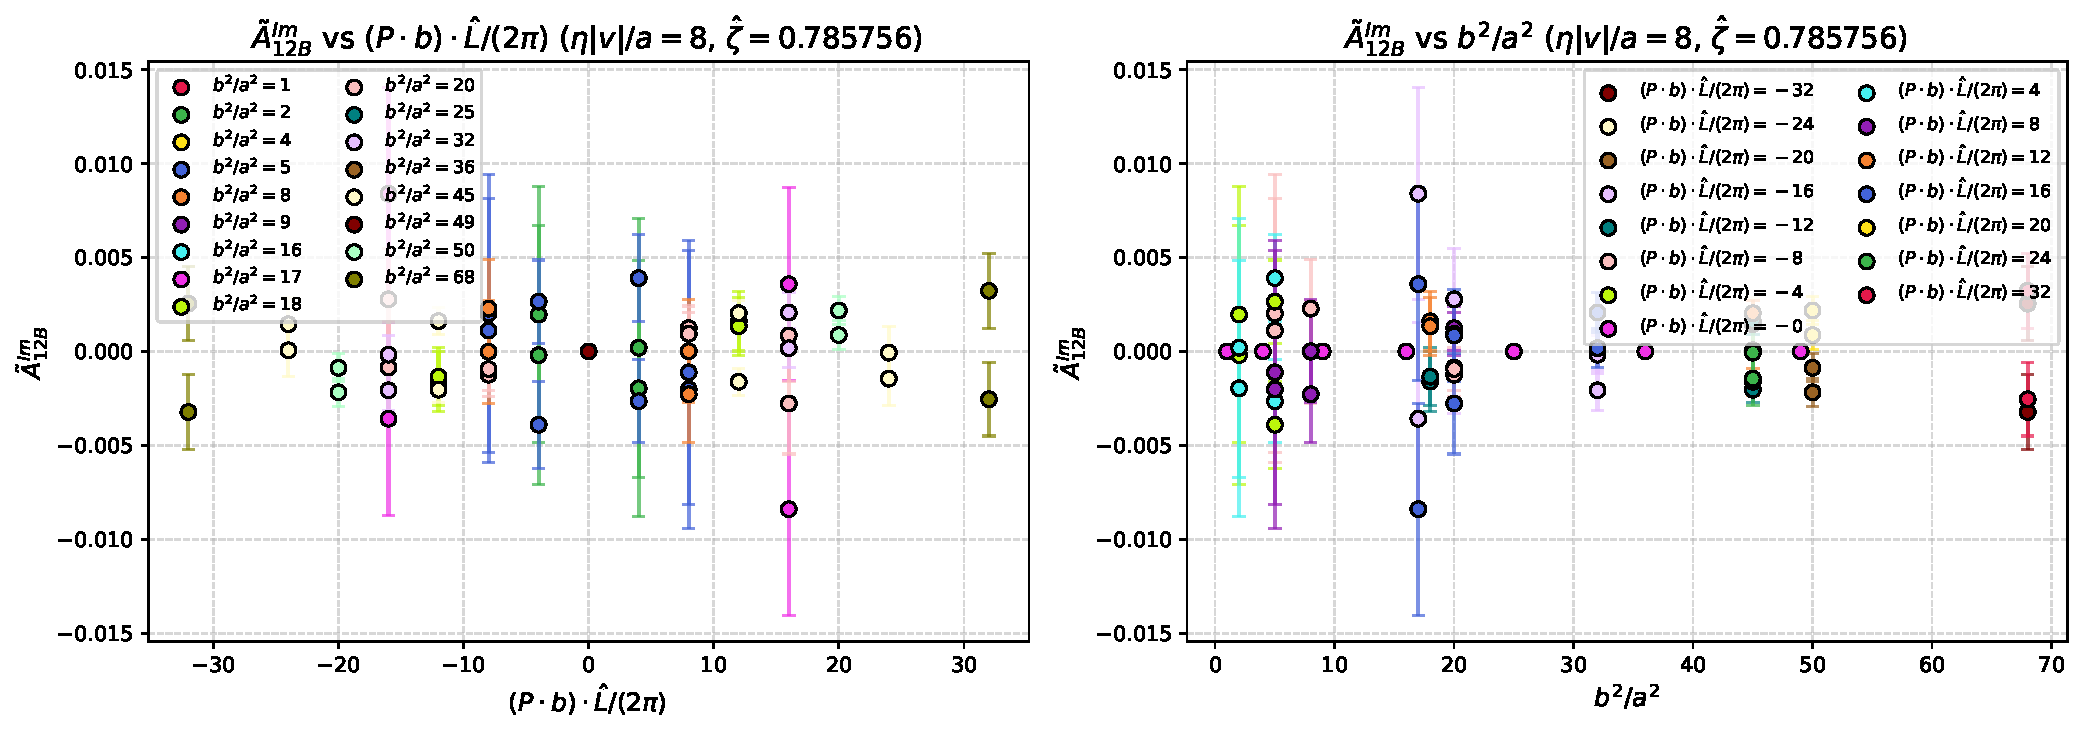
\includegraphics[width=0.98\linewidth,height=0.73\textheight,keepaspectratio]{ImA12B_Pb_bsq_eta8_PL-4_2D.pdf}\\[1mm]
{\small $\zetahat=0.785756$; $(\nu,s)$; $\eta|v|/a=8$ slices}
\figsrc{Thesis, Ch. 5: raw amplitude profiles; complete original panels.}
\end{frame}


\begin{frame}{Parity and the imaginary Sivers amplitude}
  \[
    \tAmp_{iB}^{\mathrm{Re}}(-\nu)=\tAmp_{iB}^{\mathrm{Re}}(\nu),\qquad
    \tAmp_{iB}^{\mathrm{Im}}(-\nu)=-\tAmp_{iB}^{\mathrm{Im}}(\nu).
  \]
  \begin{itemize}
    \item The profiles display the parity imposed by the amplitude projection; this is a consistency check of the extraction.
    \item The thesis finds no statistically resolved $\tAmp_{12B}^{\mathrm{Im}}$ signal and omits it from the subsequent fit. Compatibility with zero does not establish that it vanishes exactly.
    \item With this analysis choice, write $E=E_2$, $O=O_2$, $S=E_{12}$:
  \end{itemize}
  \[ \tilde f_1^{(0)}=2(E-O),\qquad
      \tilde f_{1T}^{\perp(1)}=-2S,\qquad
      \langle k_y\rangle_{TU}=-m_N\frac{S}{E-O}. \]
  \figsrc{Thesis, Ch. 5: numerical profiles and treatment of $\tAmp_{12B}^{\mathrm{Im}}$.}
\end{frame}

% Complete thesis fitting evidence in the main talk. Generated from local thesis sources.
\section{Fitting}

\begin{frame}{The fitting process: data, candidates, selection}

\begin{enumerate}
\item Test the Gaussian baseline; diagnose short-distance effects.
\item Apply $|\vect b|\ge3a$ and $6\le\eta\le10$; search with PySR.
\item Compare all Gaussian, exponential, and power-law candidates.
\item Inspect fixed-$\eta$ widths, fit statistics, and Fourier profiles.
\item Fit all three amplitudes jointly with their covariance matrix.
\item Propagate each Jackknife sample to $x$ space at $P_L=-1,-2,-3,-4$.
\end{enumerate}
\[b_L=\frac{\nu}{-P_L},\qquad b_T^2=b^2-\frac{\nu^2}{P_L^2},\qquad \nu=P\cdot b.\]
Here $b^2=|\vect b|^2\ge0$ is the spatial squared separation. The two coordinate descriptions encode the same retained data.
\figsrc{Thesis: Fitting Methodologies and Stability Analysis}
\end{frame}

\begin{frame}{Gaussian baseline: decay in the Fourier variable}

\[\tAmp_{iB}^{\mathrm{Re}}=\gamma e^{-\alpha b_L^2-\beta b_T^2}
=\gamma e^{-\beta b^2}\exp\!\left[-\frac{\alpha-\beta}{P_L^2}\nu^2\right].\]
\[\int_{-\infty}^{\infty}d\nu\,e^{ix\nu}\tAmp_{iB}^{\mathrm{Re}}
\quad\hbox{is absolutely convergent when }\alpha-\beta>0.\]
\begin{itemize}
\item $\tAmp_{2B}^{\mathrm{Re}}$: $\alpha-\beta=-0.0427(27)$, $\chi^2/\mathrm{dof}\simeq235$.
\item $\tAmp_{12B}^{\mathrm{Re}}$: $\alpha-\beta=-0.022(25)$, $\chi^2/\mathrm{dof}\simeq1.4$.
\item The unpolarized baseline fails strongly; the Sivers width difference is statistically compatible with zero and does not establish positive longitudinal damping.
\end{itemize}
\figsrc{Thesis: Fitting Methodologies and Stability Analysis}
\end{frame}

\begin{frame}{Gaussian fit: $\tAmp_{2B}^{\mathrm{Re}}$}
\centering
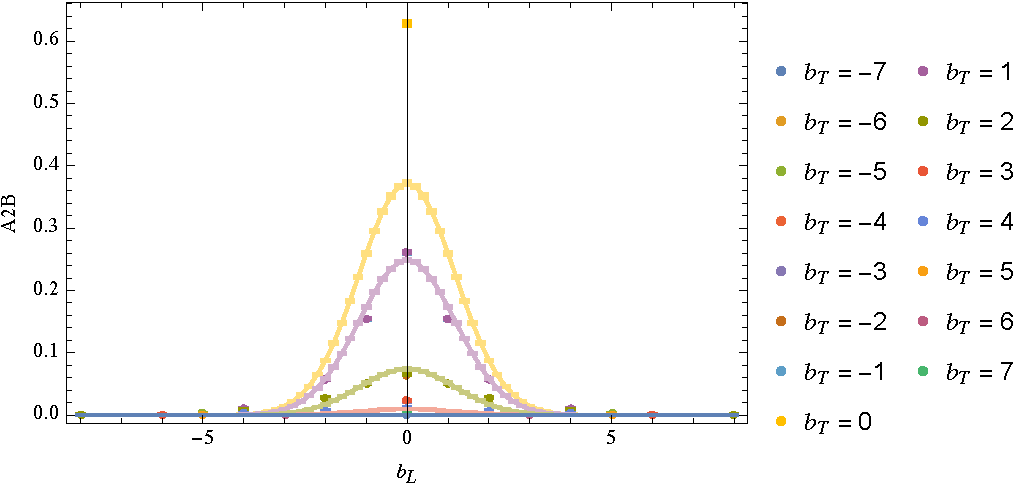
\includegraphics[width=\linewidth,height=.70\textheight,keepaspectratio]{fitting/Gaussian_A2B_Re_P1_FailedFit.pdf}

\figsrc{Thesis: plots; Gaussian\_A2B\_Re\_P1\_FailedFit}
\end{frame}

\begin{frame}{Gaussian parameters and statistics: $\tAmp_{2B}^{\mathrm{Re}}$}
\centering
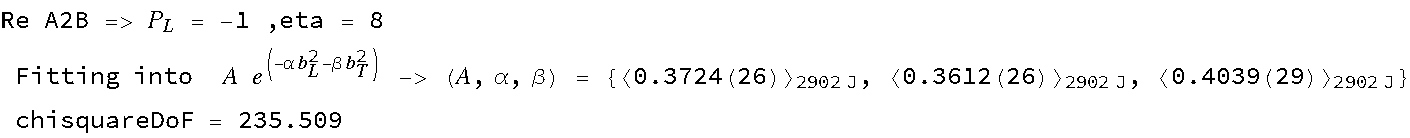
\includegraphics[width=\linewidth]{fitting/Gaussian_A2B_Re_P1_FailedFit_details1.pdf}\\[5mm]
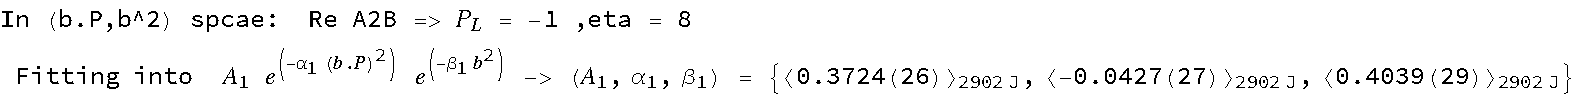
\includegraphics[width=\linewidth]{fitting/Gaussian_A2B_Re_P1_FailedFit_details2.pdf}\\[5mm]

\figsrc{Thesis: Fitting Methodologies and Stability Analysis}
\end{frame}

\begin{frame}{Gaussian fit: $\tAmp_{12B}^{\mathrm{Re}}$}
\centering
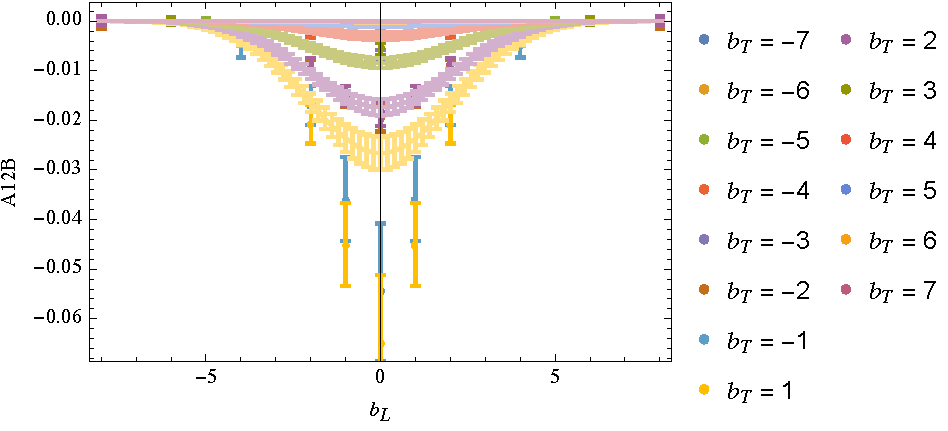
\includegraphics[width=\linewidth,height=.70\textheight,keepaspectratio]{fitting/Gaussian_A12B_Re_P1_FailedFit.pdf}

\figsrc{Thesis: plots; Gaussian\_A12B\_Re\_P1\_FailedFit}
\end{frame}

\begin{frame}{Gaussian parameters and statistics: $\tAmp_{12B}^{\mathrm{Re}}$}
\centering
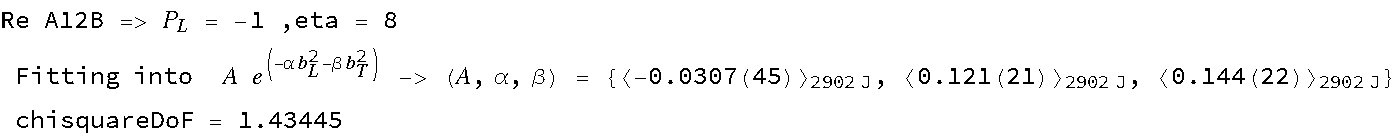
\includegraphics[width=\linewidth]{fitting/Gaussian_A12B_Re_P1_FailedFit_details1.pdf}\\[5mm]
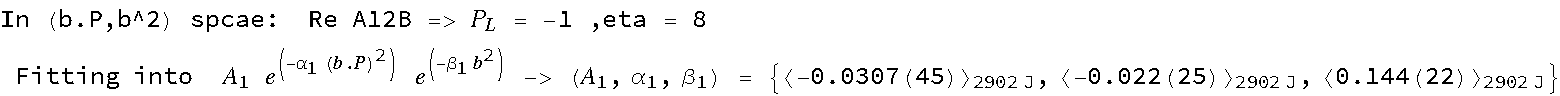
\includegraphics[width=\linewidth]{fitting/Gaussian_A12B_Re_P1_FailedFit_details2.pdf}\\[5mm]

\figsrc{Thesis: Fitting Methodologies and Stability Analysis}
\end{frame}

\begin{frame}{Short-distance diagnostic and the spatial cut}
\centering
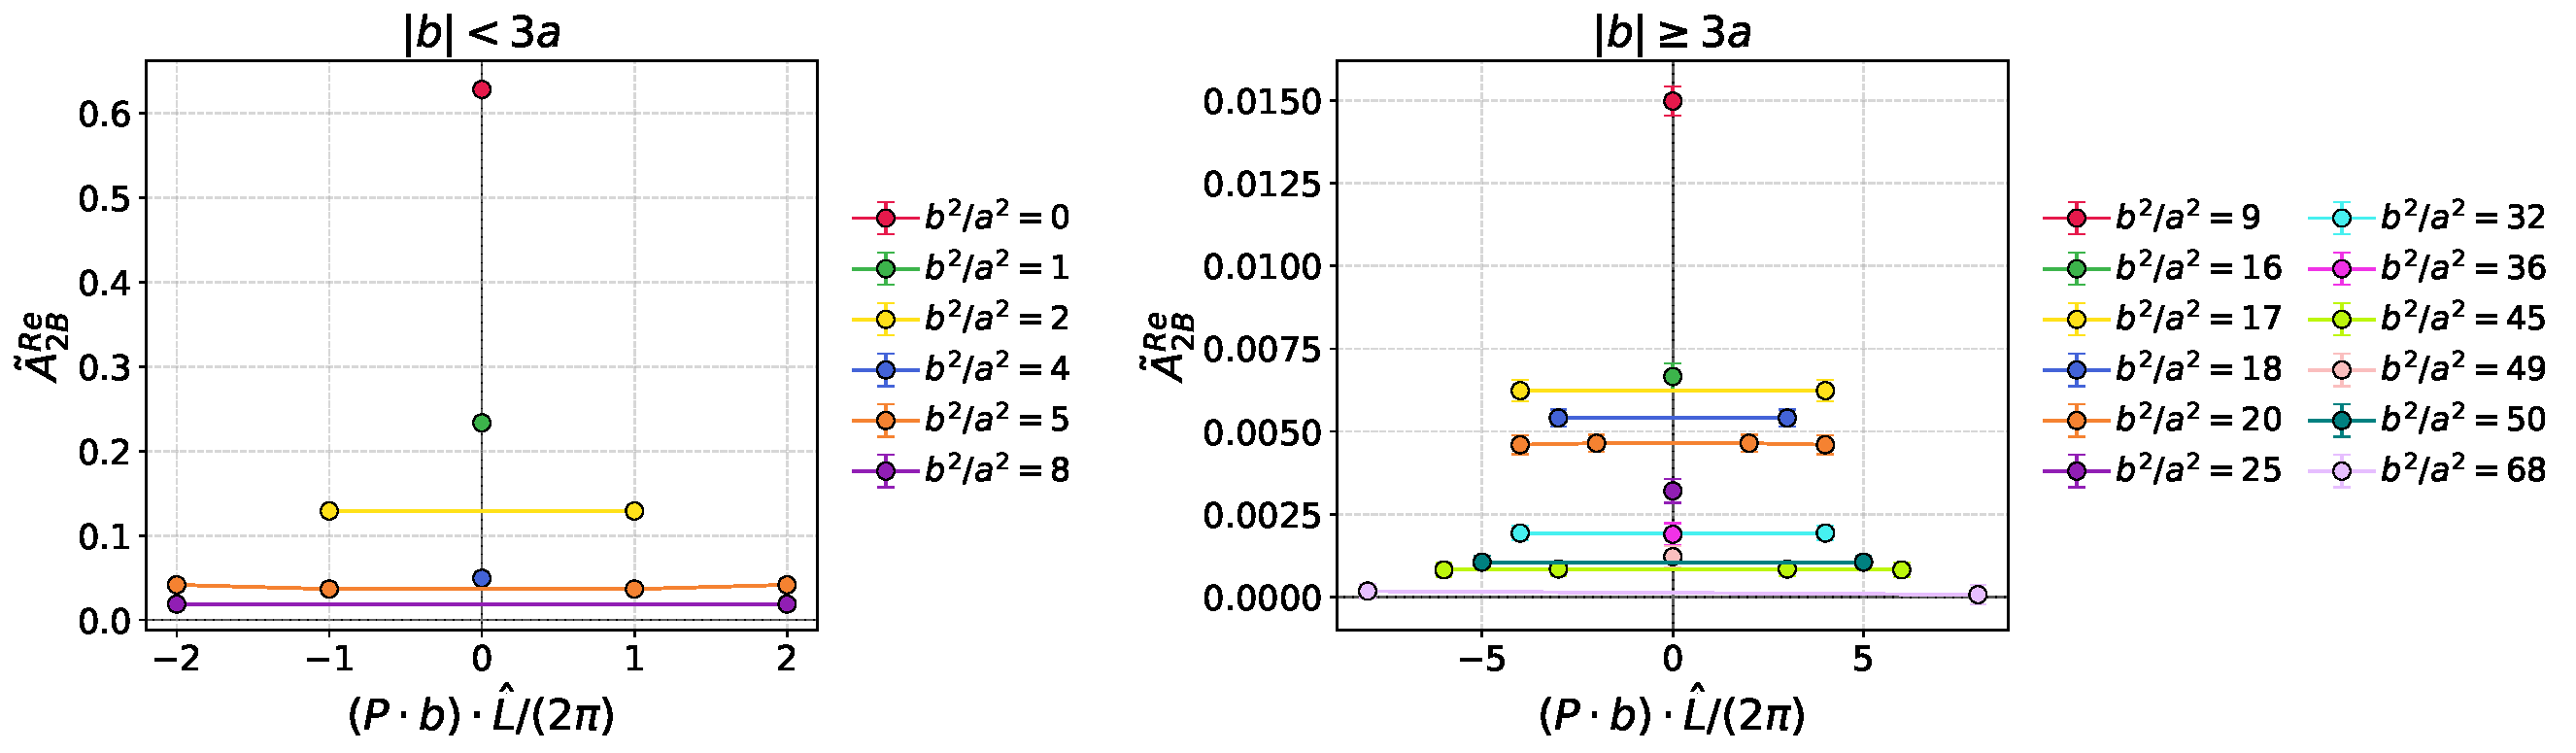
\includegraphics[width=\linewidth,height=.70\textheight,keepaspectratio]{fitting/A2B_Re_b_lessthan3_and_ge3.pdf}
\par\small At $P_L=-1$, $\eta|v|/a=9$, the $b^2/a^2=5$ group rises by about $14\%$. Retain $|\vect b|\ge3a$ in all subsequent fits; this reduces short-distance contamination but does not remove all finite-$a$ effects.

\figsrc{Thesis: plots; A2B\_Re\_b\_lessthan3\_and\_ge3}
\end{frame}

\begin{frame}{Global fit domain and staple dependence}

\[|\vect b|=\sqrt{b_L^2+b_T^2}\ge3a,\qquad6\le\eta|v|/a\le10.\]
\begin{itemize}
\item Fit the full $(b_L,b_T,\eta)$ grid at each fixed nucleon momentum.
\item A common $e^{-f\eta}$ factor is imposed in the final three-amplitude model and cancels in the Sivers ratio.
\item Residual $\eta$ dependence of the real unpolarized width is retained before taking $\eta\to\infty$.
\item The continuation to arbitrary $\nu$ at fixed $b^2$ extends beyond the measured spatial domain $\nu^2\le P_L^2 b^2$; its functional form is a model assumption.
\end{itemize}
\figsrc{Thesis: Fitting Methodologies and Stability Analysis}
\end{frame}

\begin{frame}{PySR: complete search configuration}

\small\renewcommand{\arraystretch}{1.35}
\begin{tabular}{ll}\toprule
Inputs & $\eta,b_L,b_T$; target $\tAmp_{2B}^{\mathrm{Re}}$, $P_L=-1$\\
Binary operators & $+,-,\times,/,\ \operatorname{pow}(u,v)=u^v$\\
Custom binary operator & $\operatorname{lor}(u,v)=(1+u^2+v^2)^{-2}$\\
Unary operators & $u^2,\ \exp(u),\ \operatorname{decay}(u)=e^{-u}$\\
Operator constraints & $\operatorname{pow}:(-1,1)$; $\operatorname{lor}:(10,10)$; decay: $10$\\
Forbidden nesting & exp inside exp; decay inside decay; decay inside exp\\
Populations / iterations & $30\,/\,100$\\
Maximum tree complexity & $28$\\
Regularization weight & $\epsilon=0.1$\\\bottomrule
\end{tabular}
\par\medskip The search explores expression trees; operator choices favor some families over others.
\figsrc{Thesis: PySR configuration; target momentum corrected to match chapter and plots}
\end{frame}

\begin{frame}{PySR loss: the implemented objective}

\[\mathcal L=\frac{1}{N_{\rm data}-3}\sum_{i=1}^{N_{\rm data}}
\frac{[F(\eta_i,b_{L,i},b_{T,i})-y_i]^2}{\sigma_i^2}
+0.1\sum_{p\in\mathcal P}F(p)^2.\]
\[\mathcal P=\{(10,50,1),(10,80,1),(10,10,1),(8,20,1),(6,30,2)\},\]
where each tuple is $(\eta,b_L/a,b_T/a)$.
\begin{itemize}
\item Invalid data predictions return infinite loss; an invalid penalty prediction adds $10^6$ before multiplication by $0.1$.
\item These finite probes discourage large predictions; they do not prove convergence of an infinite Fourier integral.
\item The source code uses squared predictions and a fixed $N_{\rm data}-3$ normalization. Reported loss is therefore not a model-by-model reduced $\chi^2$.
\end{itemize}
\figsrc{Thesis: exact objective in PySR outputs / custom loss Julia listing}
\end{frame}

\begin{frame}{PySR Pareto front: stored candidates (1/7)}
\small $B=1+b_L^2+b_T^2$, $L(u,v)=(1+u^2+v^2)^{-2}$.\par\medskip\renewcommand{\arraystretch}{2.0}\begin{tabular}{ccl}\toprule $C$ & Loss & Exact stored expression\\\midrule
1 & 276.43433 & $0.005040839$ \\
3 & 171.56175 & $0.49875718^\eta$ \\
4 & 167.5698 & $e^{-\eta^{0.80833286}}$ \\
5 & 130.85486 & $34.16954\,L(\eta,b_L)$ \\\bottomrule\end{tabular}
\figsrc{Source: PySR outputs\_A2B\_real / 20260821\_101855\_eCTY5z / hall\_of\_fame.csv}
\end{frame}

\begin{frame}{PySR Pareto front: stored candidates (2/7)}
\small $B=1+b_L^2+b_T^2$, $L(u,v)=(1+u^2+v^2)^{-2}$.\par\medskip\renewcommand{\arraystretch}{2.0}\begin{tabular}{ccl}\toprule $C$ & Loss & Exact stored expression\\\midrule
7 & 68.93352 & $(11.584338-\eta)B^{-2}$ \\
9 & 30.807978 & $(10.156917-\eta)B^{-1.7775426}$ \\
11 & 5.158913 & $(7.0522256/\eta)^4 B^{-1.44250464}$ \\
12 & 4.7633114 & $[(\eta-14.485626)/\eta]^2 B^{-1.4604364}$ \\\bottomrule\end{tabular}
\figsrc{Source: PySR outputs\_A2B\_real / 20260821\_101855\_eCTY5z / hall\_of\_fame.csv}
\end{frame}

\begin{frame}{PySR Pareto front: stored candidates (3/7)}
\small $B=1+b_L^2+b_T^2$, $L(u,v)=(1+u^2+v^2)^{-2}$.\par\medskip\renewcommand{\arraystretch}{2.0}\begin{tabular}{ccl}\toprule $C$ & Loss & Exact stored expression\\\midrule
14 & 3.934378 & $\frac{e^{-0.534084(\eta-8.68932)}}{2.6322825\,B^{1.390951}}$ \\
16 & 2.0260298 & $\frac{e^{-0.46820307(\eta-8.994358)}}{3.5930288\,B^{1.2585272}}-0.0012706916$ \\\bottomrule\end{tabular}
\figsrc{Source: PySR outputs\_A2B\_real / 20260821\_101855\_eCTY5z / hall\_of\_fame.csv}
\end{frame}

\begin{frame}{PySR Pareto front: stored candidates (4/7)}
\small $B=1+b_L^2+b_T^2$, $L(u,v)=(1+u^2+v^2)^{-2}$.\par\medskip\renewcommand{\arraystretch}{2.0}\begin{tabular}{ccl}\toprule $C$ & Loss & Exact stored expression\\\midrule
17 & 1.9917132 & $\left(\frac{10.461691}{\eta}\right)^{2.3353815}\frac{B^{-1.2146622}}{0.593981\eta}-0.0016621732$ \\
18 & 1.9095322 & $\frac{B^{-1.251997}}{1.4630643}\left(\frac{17.983559-\eta}{-1.560787\eta}\right)^2-0.0013669281$ \\\bottomrule\end{tabular}
\figsrc{Source: PySR outputs\_A2B\_real / 20260821\_101855\_eCTY5z / hall\_of\_fame.csv}
\end{frame}

\begin{frame}{PySR Pareto front: stored candidates (5/7)}
\small $B=1+b_L^2+b_T^2$, $L(u,v)=(1+u^2+v^2)^{-2}$.\par\medskip\renewcommand{\arraystretch}{2.0}\begin{tabular}{ccl}\toprule $C$ & Loss & Exact stored expression\\\midrule
19 & 1.7628223 & $\frac1\eta\left(\frac{10.381556}{\eta}\right)^{2.369394}\left(\frac{B^{-1.1273306}}{0.7187267}-0.0032199204\right)-0.0014922422$ \\
21 & 1.7604288 & $\frac1\eta\left(\frac{10.300505}{\eta}\right)^{2.4254909}\left(\frac{B^{-1.1335096}}{0.71366495}-0.003188983\right)-0.001388529$ \\\bottomrule\end{tabular}
\figsrc{Source: PySR outputs\_A2B\_real / 20260821\_101855\_eCTY5z / hall\_of\_fame.csv}
\end{frame}

\begin{frame}{PySR Pareto front: stored candidates (6/7)}
\small $L(u,v)=(1+u^2+v^2)^{-2}$; these higher-complexity stored candidates were omitted from the thesis table.\par
\[\Delta_{22}=b_L-L(-0.1626809,b_L^2),\qquad\mathcal L_{22}=1.6167384.\]
\[F_{22}=\frac{L(\Delta_{22},b_T)^{0.66107386}}{\eta}\left(\frac{14.42762}{\eta+0.12903585}\right)^{2.5097084}-0.0012624399.\]
\[\Delta_{23}=b_L-L(b_L,0.213843),\qquad\mathcal L_{23}=1.5782435.\]
\[F_{23}=\frac{2.7467434\,L(b_T,\Delta_{23})^{0.6493724}}{\eta}\left(\frac{10.018184}{\eta+0.7164768}\right)^{2.6639583}-0.0013878929.\]
These shifted spatial profiles are not even in $b_L$; they require a symmetry check before physical use.
\figsrc{Source: PySR outputs\_A2B\_real / 20260821\_101855\_eCTY5z / hall\_of\_fame.csv}
\end{frame}

\begin{frame}{PySR Pareto front: stored candidates (7/7)}
\small $L(u,v)=(1+u^2+v^2)^{-2}$; these higher-complexity stored candidates were omitted from the thesis table.\par
\[\Delta_{25}=b_L-L(b_L,0.04371186\eta),\qquad\mathcal L_{25}=1.5110264.\]
\[F_{25}=\frac{2.7467434\,L(\Delta_{25},b_T)^{0.6493724}}{\eta}\left(\frac{10.018184}{\eta+0.7164768}\right)^{2.6639583}-0.0013878929.\]
\[\Delta_{27}=b_L-L(2b_L,0.04371186\eta),\qquad\mathcal L_{27}=1.5023776.\]
\[F_{27}=\frac{2.7467434\,L(b_T,\Delta_{27})^{0.6493724}}{\eta}\left(\frac{10.018184}{\eta+0.7164768}\right)^{2.6639583}-0.0013878929.\]
These shifted spatial profiles are not even in $b_L$; they require a symmetry check before physical use.
\figsrc{Source: PySR outputs\_A2B\_real / 20260821\_101855\_eCTY5z / hall\_of\_fame.csv}
\end{frame}

\begin{frame}{PySR benchmark models: panels 1 and 2}
\centering
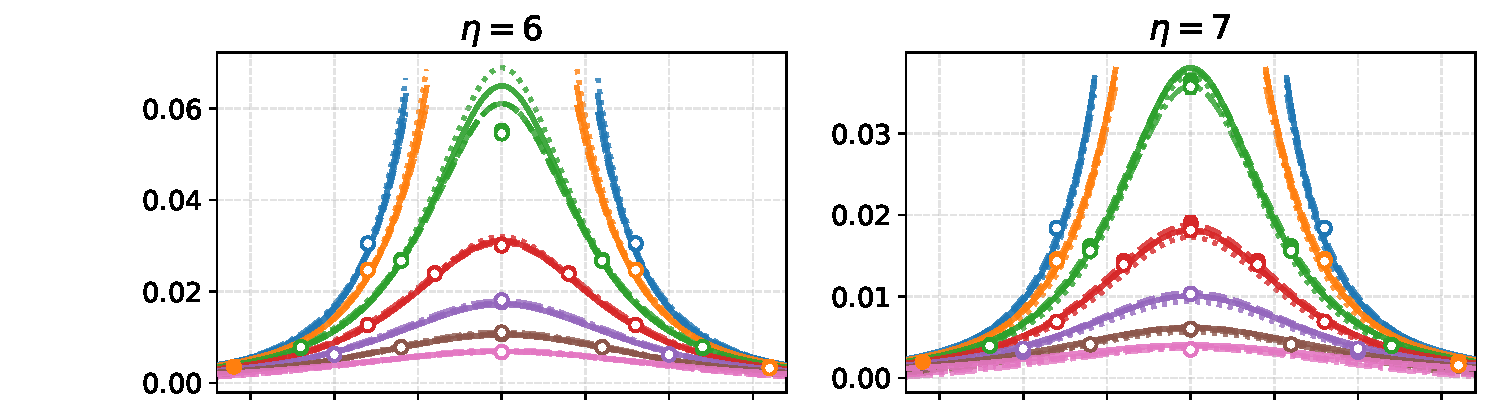
\includegraphics[width=\linewidth,height=.70\textheight,keepaspectratio]{fitting/01_A2B_PySR_Benchmark_Fits__row1.pdf}
\par\small All four overlays: $C=11,14,16,17$; curves restricted to $|\vect b|\ge3a$.

\figsrc{Thesis: PySR\_outputs; 01\_A2B\_PySR\_Benchmark\_Fits}
\end{frame}

\begin{frame}{PySR benchmark models: panels 3 and 4}
\centering
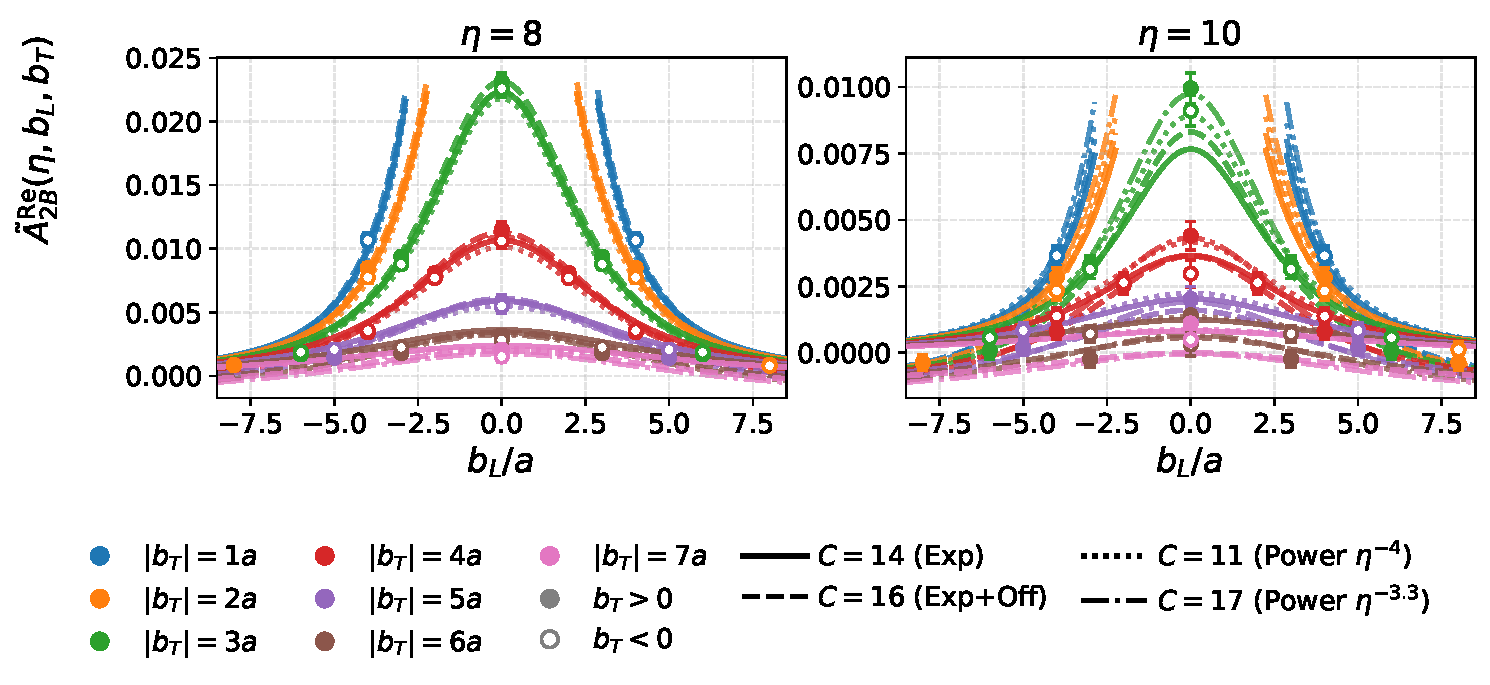
\includegraphics[width=\linewidth,height=.70\textheight,keepaspectratio]{fitting/01_A2B_PySR_Benchmark_Fits__row2.pdf}
\par\small All four overlays: $C=11,14,16,17$; curves restricted to $|\vect b|\ge3a$.

\figsrc{Thesis: PySR\_outputs; 01\_A2B\_PySR\_Benchmark\_Fits}
\end{frame}

\begin{frame}{Gaussian straight-line diagnostic}
\centering
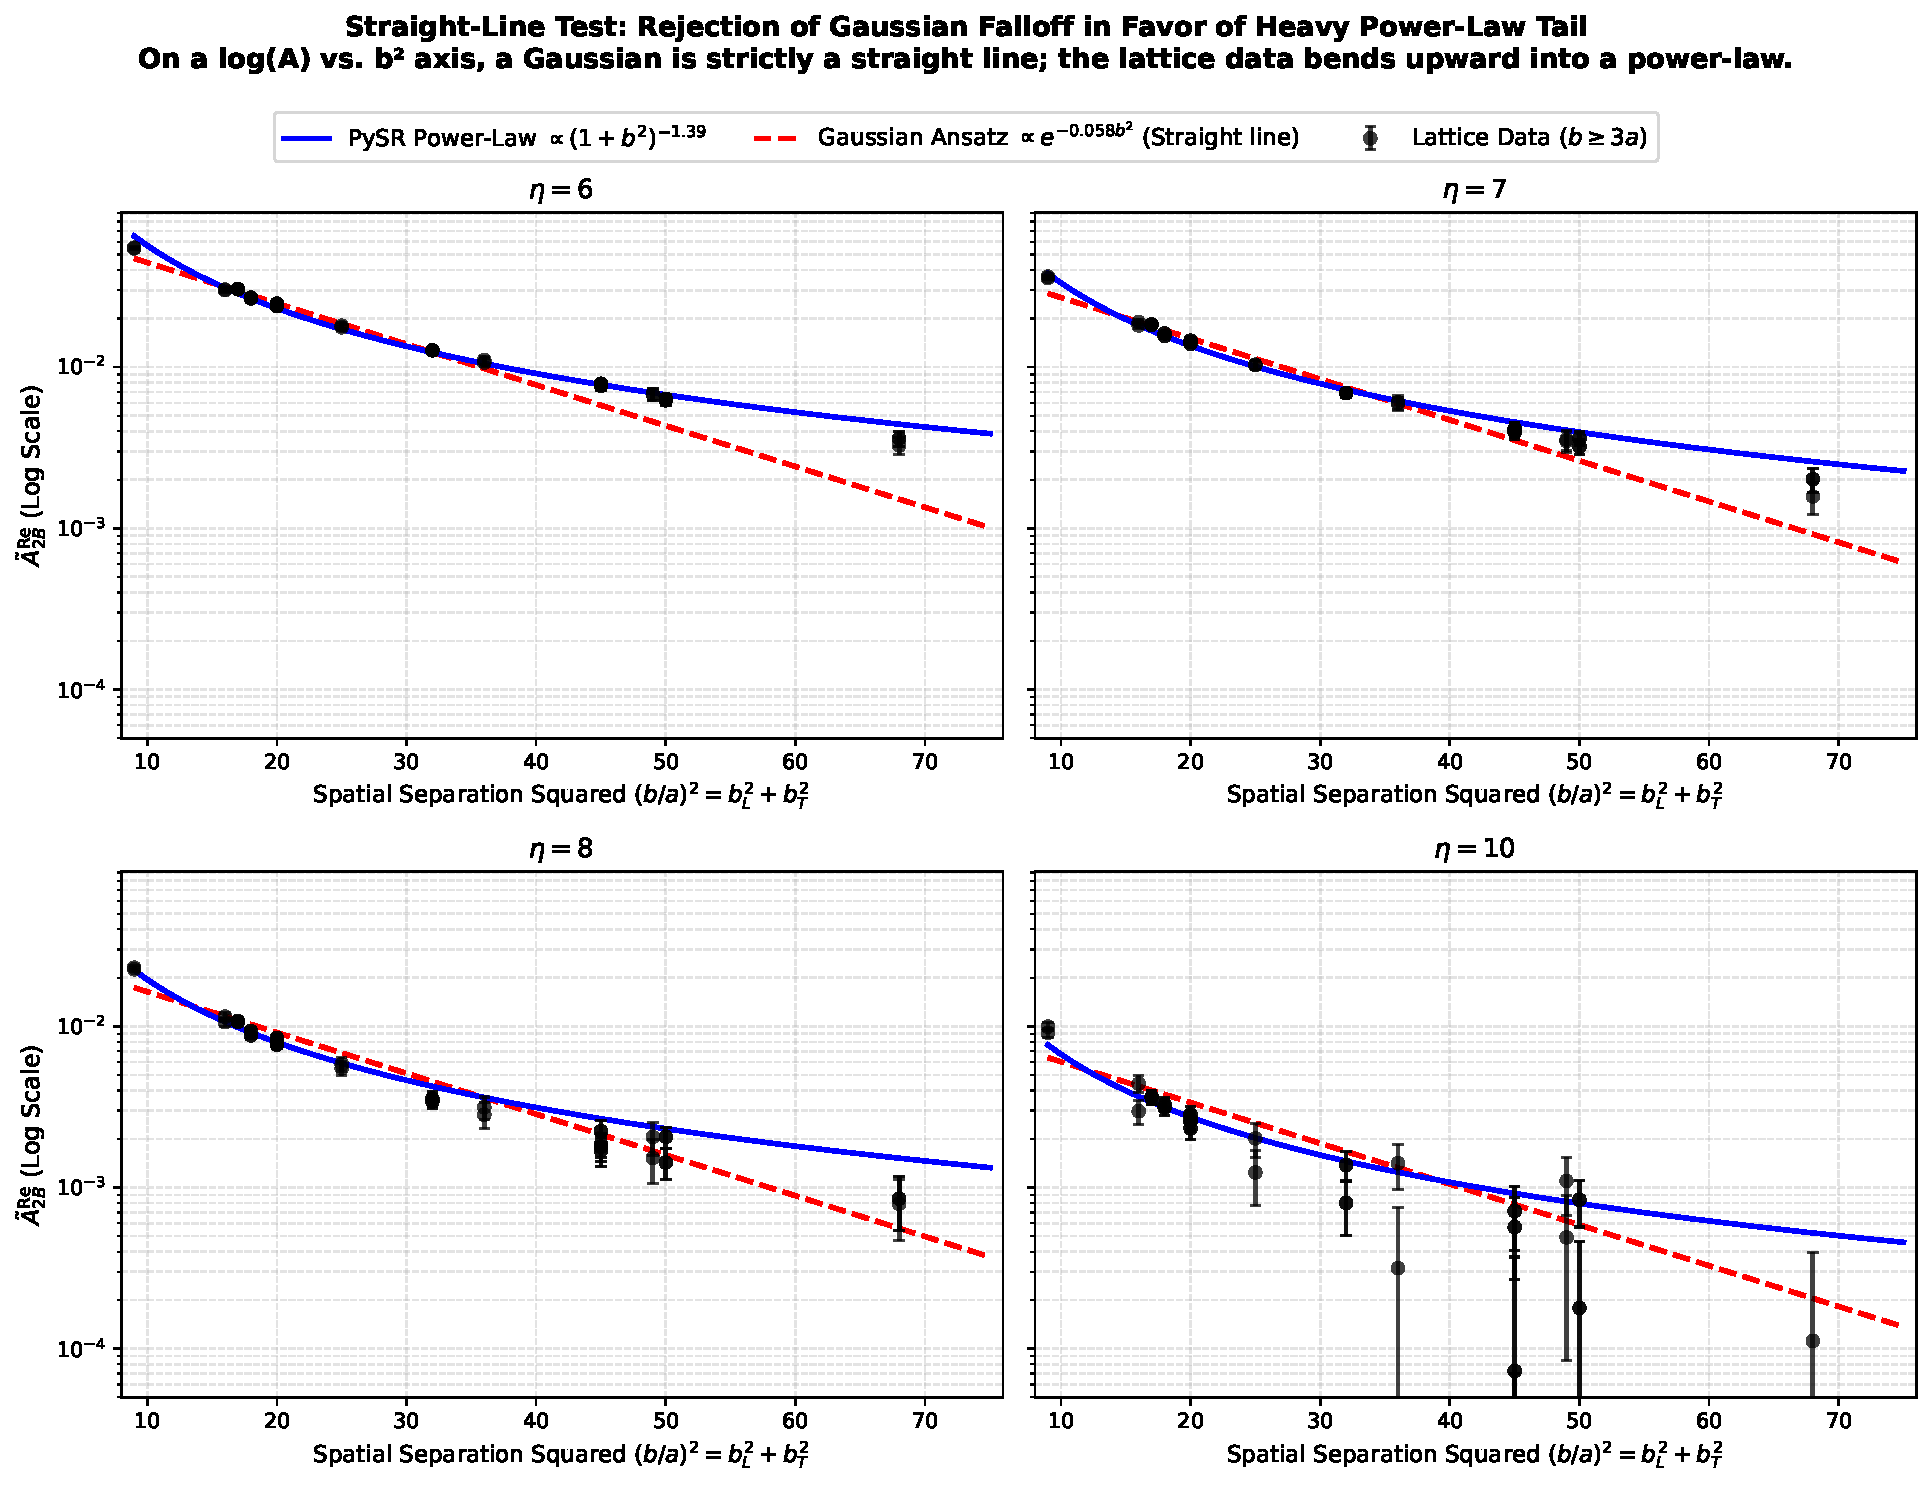
\includegraphics[width=\linewidth,height=.70\textheight,keepaspectratio]{fitting/02_Gaussian_StraightLine_Test.pdf}
\par\small $\log\tAmp_{2B}^{\mathrm{Re}}$ versus $b^2$: the data bend away from the Gaussian baseline ($c=0.058$).

\figsrc{Thesis: PySR\_outputs; 02\_Gaussian\_StraightLine\_Test}
\end{frame}

\begin{frame}{What symbolic regression establishes}

\[F_{14}=\frac{39.36887e^{-0.534084\eta}}{(1+b^2)^{1.390951}},\qquad
F_{16}=\frac{18.76870e^{-0.46820307\eta}}{(1+b^2)^{1.2585272}}-0.0012706916.\]
\begin{itemize}
\item A power-law spatial envelope and an exponential staple profile describe the retained finite grid.
\item At fixed $b^2$, the thesis-highlighted $C=14,16$ expressions have no $\nu=P\cdot b$ dependence. They are guides to the final model, not directly usable ordinary Fourier-integrable longitudinal profiles.
\item Nonzero offsets also survive at large spatial separation; the finite-probe loss does not enforce exact decay to zero.
\item Exact stored formulas correct the thesis prefactors ($39.71$, $245.5$) and the $C=21$ grouping. Higher-complexity stored candidates also need an even-parity check.\item No square-root operator was provided: $e^{-c|\vect b|}$ is more costly for this search to construct.
\end{itemize}
\figsrc{Thesis: Fitting Methodologies and Stability Analysis}
\end{frame}

\begin{frame}{Exponential spatial decay remains competitive}
\centering
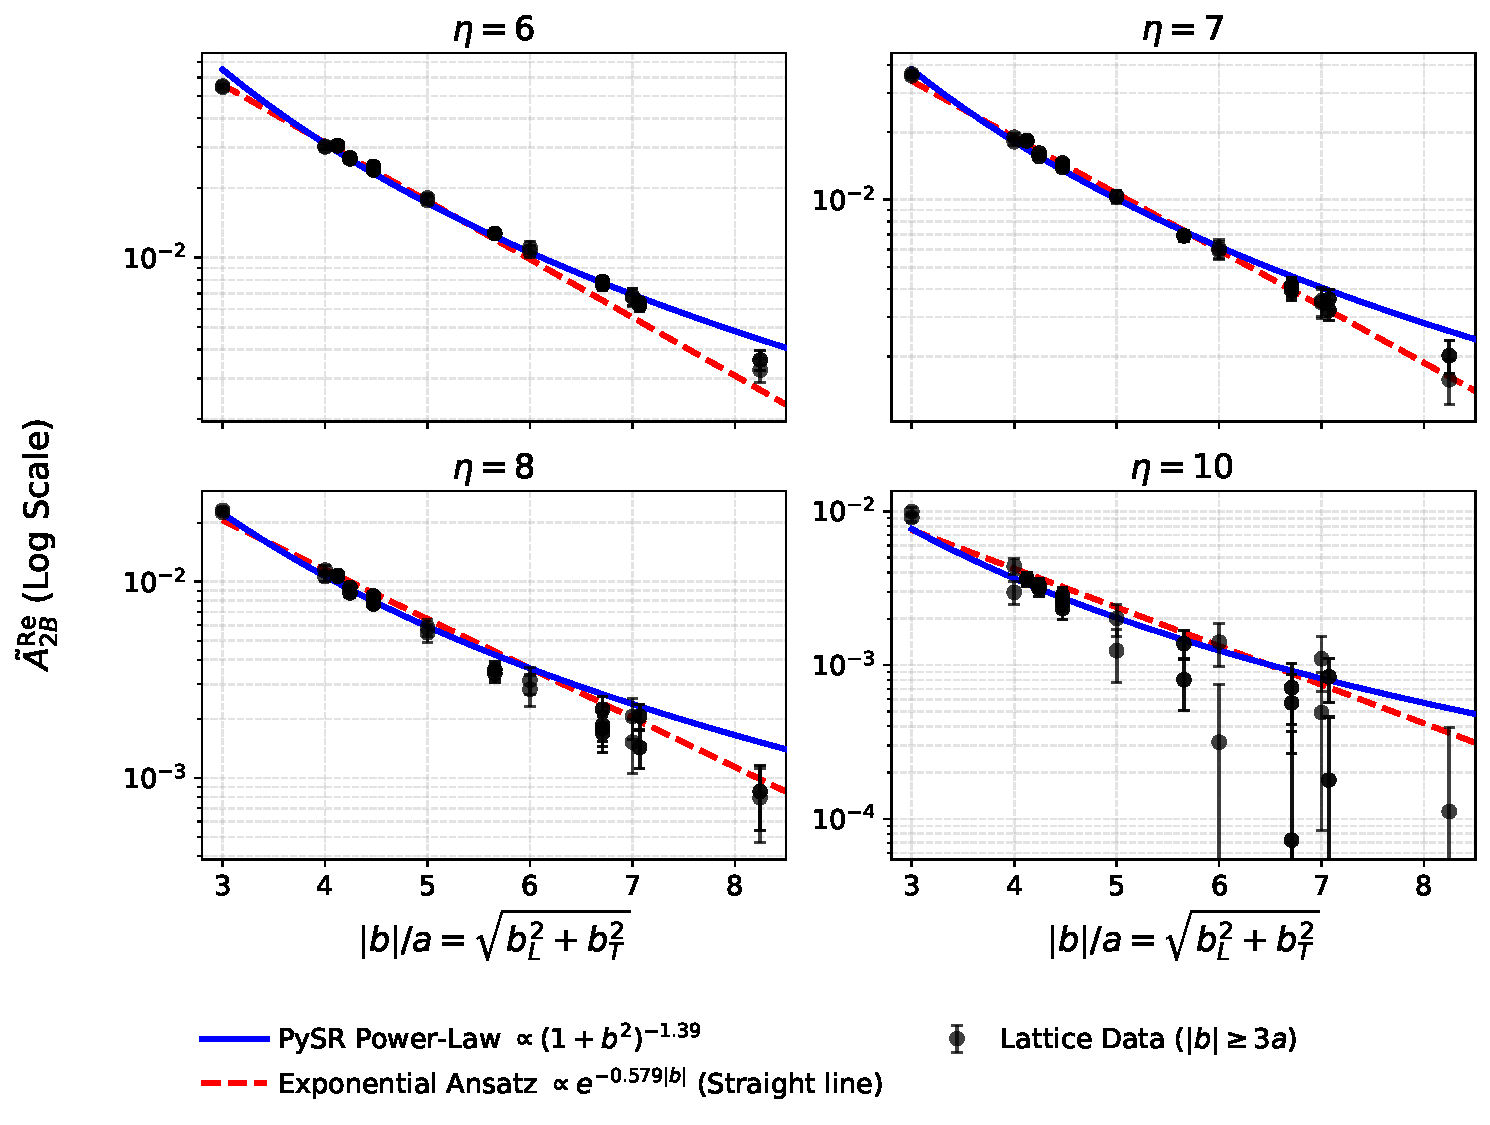
\includegraphics[width=\linewidth,height=.70\textheight,keepaspectratio]{fitting/03_Exponential_b_StraightLine_Test.pdf}
\par\small $e^{-c|\vect b|}$ with $c=0.579$ describes the real unpolarized data over $3\le|\vect b|/a\le8.2$. Direct losses: about $2.63$, or $2.26$ with an offset.

\figsrc{Thesis: PySR\_outputs; 03\_Exponential\_b\_StraightLine\_Test}
\end{frame}

\begin{frame}{Separable real-unpolarized candidates: constant width --- models}
\centering
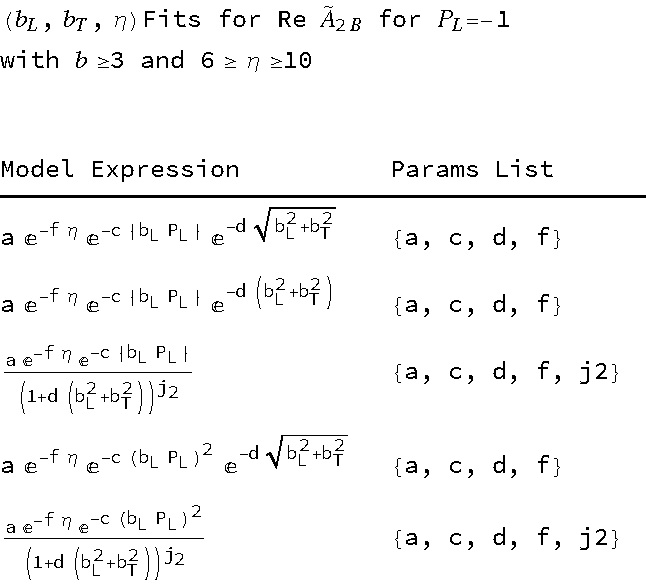
\includegraphics[width=\linewidth,height=.70\textheight,keepaspectratio]{fitting/Rejection-of-Separable-Exponential-Longitudinal-Decay__part1.pdf}
\par\small Five tested forms; all parameter values and $\chi^2/\mathrm{dof}$ retained. Correct cut: $6\le\eta\le10$.

\figsrc{Thesis: plots; Rejection-of-Separable-Exponential-Longitudinal-Decay}
\end{frame}

\begin{frame}{Separable real-unpolarized candidates: constant width --- fit results}
\centering
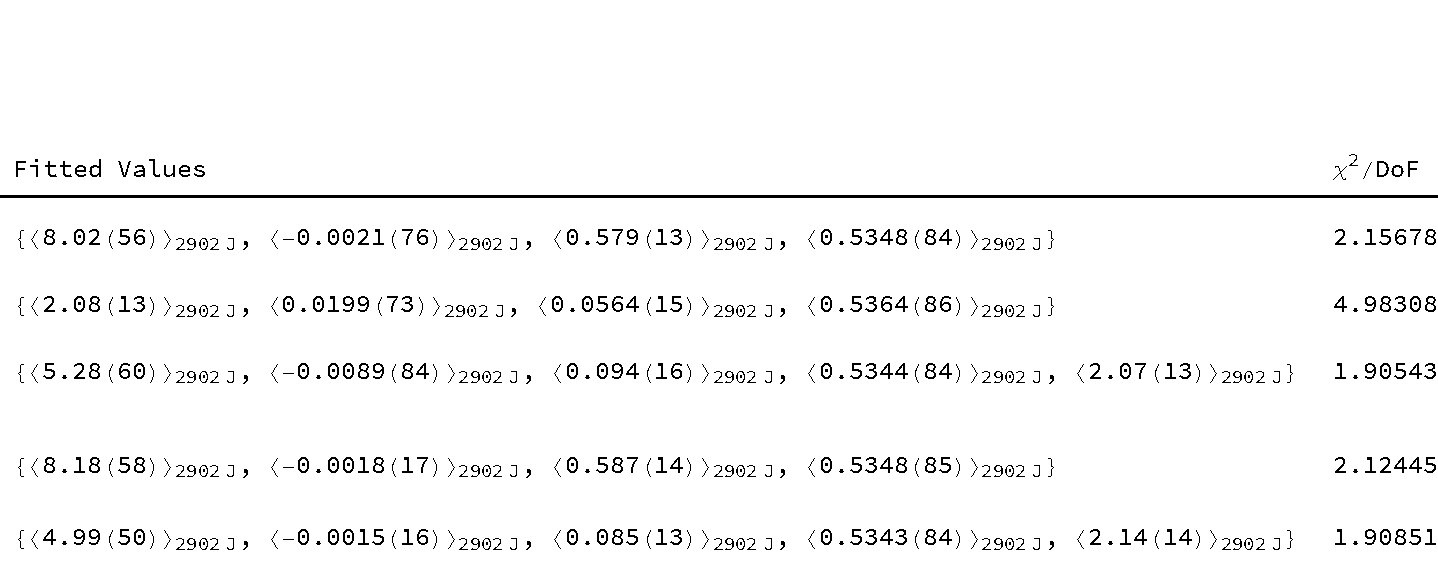
\includegraphics[width=\linewidth,height=.70\textheight,keepaspectratio]{fitting/Rejection-of-Separable-Exponential-Longitudinal-Decay__part2.pdf}
\par\small Five tested forms; all parameter values and $\chi^2/\mathrm{dof}$ retained. Correct cut: $6\le\eta\le10$.

\figsrc{Thesis: plots; Rejection-of-Separable-Exponential-Longitudinal-Decay}
\end{frame}

\begin{frame}{Separable real-unpolarized candidates: variable width --- models}
\centering
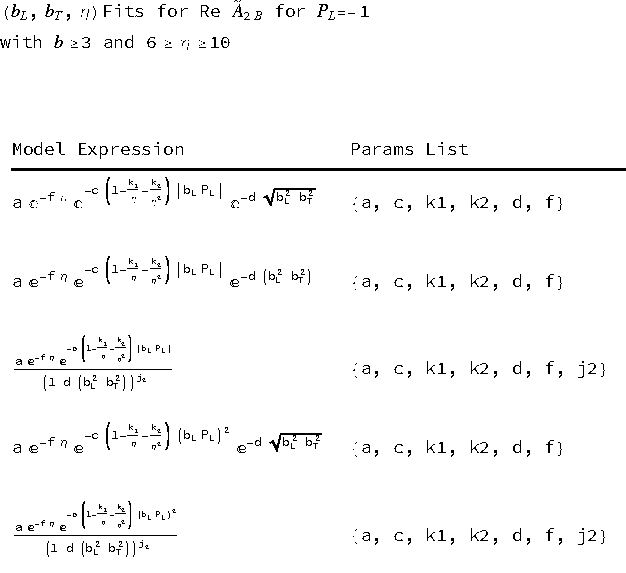
\includegraphics[width=\linewidth,height=.70\textheight,keepaspectratio]{fitting/Rejection-of-Separable-Exponential-Longitudinal-Decay-ceta__part1.pdf}
\par\small Five tested forms; all parameter values and $\chi^2/\mathrm{dof}$ retained. Correct cut: $6\le\eta\le10$.

\figsrc{Thesis: plots; Rejection-of-Separable-Exponential-Longitudinal-Decay-ceta}
\end{frame}

\begin{frame}{Separable real-unpolarized candidates: variable width --- fit results}
\centering
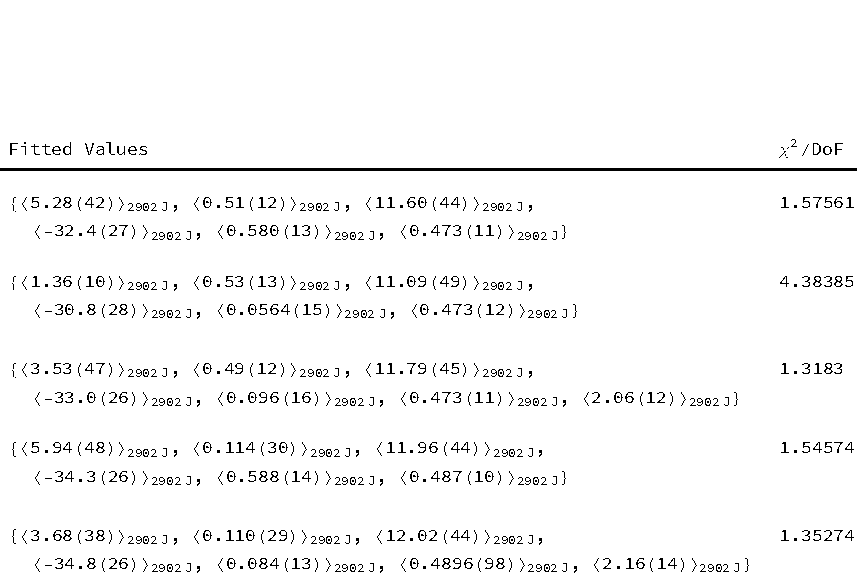
\includegraphics[width=\linewidth,height=.70\textheight,keepaspectratio]{fitting/Rejection-of-Separable-Exponential-Longitudinal-Decay-ceta__part2.pdf}
\par\small Five tested forms; all parameter values and $\chi^2/\mathrm{dof}$ retained. Correct cut: $6\le\eta\le10$.

\figsrc{Thesis: plots; Rejection-of-Separable-Exponential-Longitudinal-Decay-ceta}
\end{frame}

\begin{frame}{Sixteen Gaussian candidates: the full family}

\[F_{rs}=a e^{-f\eta}\exp[-c\,g_r(\eta;k_1,k_2)\nu^2-d\,g_s(\eta;l_1,l_2)b^2],\]
\[\begin{aligned}
g_0(\eta;u,v)&=1,&g_1(\eta;u,v)&=1-\frac{u}{\eta},\\
g_2(\eta;u,v)&=1+\frac{u}{\eta}-\frac{v}{\sqrt\eta},&
g_3(\eta;u,v)&=1-\frac{u}{\eta}-\frac{v}{\eta^2}.
\end{aligned}\]
\[\begin{array}{c|cccc}
 &g_0(d)&g_1(d)&g_2(d)&g_3(d)\\\hline
 g_0(c)&1&5&6&7\\g_1(c)&2&8&9&10\\g_2(c)&3&11&12&13\\g_3(c)&4&14&15&16
\end{array}\]
Numbers identify the original table rows. The next slides retain every expression, parameter estimate, and fit statistic.
\figsrc{Thesis: Fitting Methodologies and Stability Analysis}
\end{frame}

\begin{frame}{Gaussian candidates --- block 1, models}
\centering
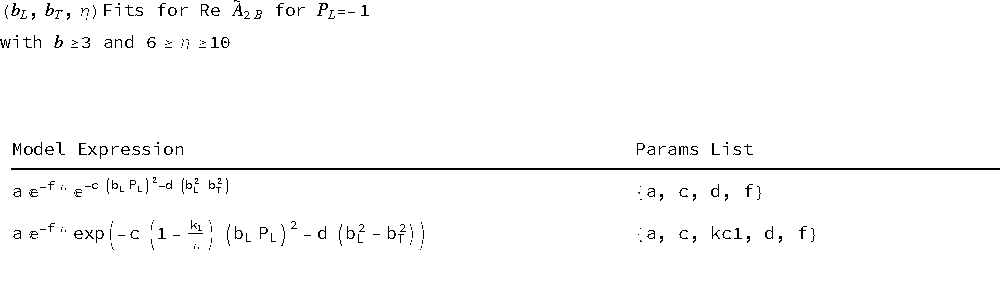
\includegraphics[width=\linewidth,height=.72\textheight,keepaspectratio]{fitting/fit_list_gaussian_c_d_etas__block1_part1.pdf}
\par\small $P_L=-1$, $|\vect b|\ge3a$, $6\le\eta\le10$. Original thesis table, enlarged without omitted rows.

\figsrc{Thesis: plots; fit\_list\_gaussian\_c\_d\_etas}
\end{frame}

\begin{frame}{Gaussian candidates --- block 1, parameters and diagnostics}
\centering
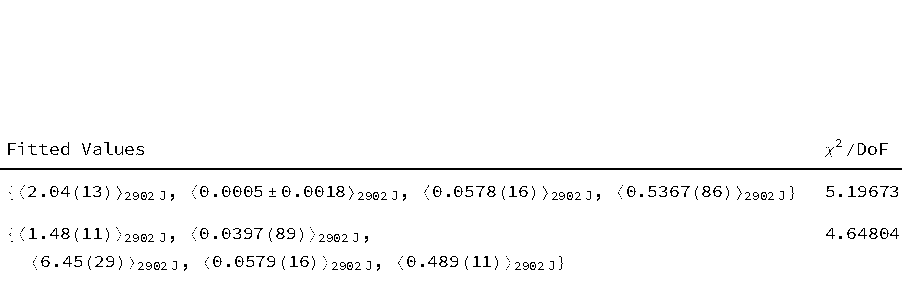
\includegraphics[width=\linewidth,height=.72\textheight,keepaspectratio]{fitting/fit_list_gaussian_c_d_etas__block1_part2.pdf}
\par\small $P_L=-1$, $|\vect b|\ge3a$, $6\le\eta\le10$. Original thesis table, enlarged without omitted rows.

\figsrc{Thesis: plots; fit\_list\_gaussian\_c\_d\_etas}
\end{frame}

\begin{frame}{Gaussian candidates --- block 2, models}
\centering
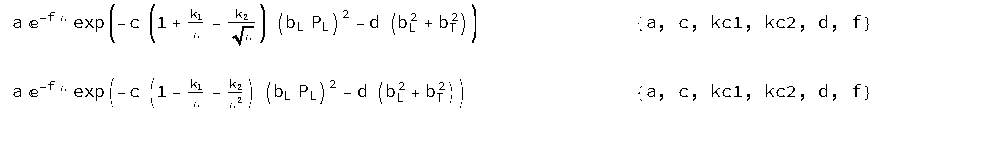
\includegraphics[width=\linewidth,height=.72\textheight,keepaspectratio]{fitting/fit_list_gaussian_c_d_etas__block2_part1.pdf}
\par\small $P_L=-1$, $|\vect b|\ge3a$, $6\le\eta\le10$. Original thesis table, enlarged without omitted rows.

\figsrc{Thesis: plots; fit\_list\_gaussian\_c\_d\_etas}
\end{frame}

\begin{frame}{Gaussian candidates --- block 2, parameters and diagnostics}
\centering
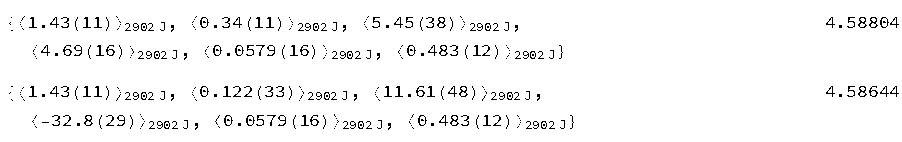
\includegraphics[width=\linewidth,height=.72\textheight,keepaspectratio]{fitting/fit_list_gaussian_c_d_etas__block2_part2.pdf}
\par\small $P_L=-1$, $|\vect b|\ge3a$, $6\le\eta\le10$. Original thesis table, enlarged without omitted rows.

\figsrc{Thesis: plots; fit\_list\_gaussian\_c\_d\_etas}
\end{frame}

\begin{frame}{Gaussian candidates --- block 3, models}
\centering
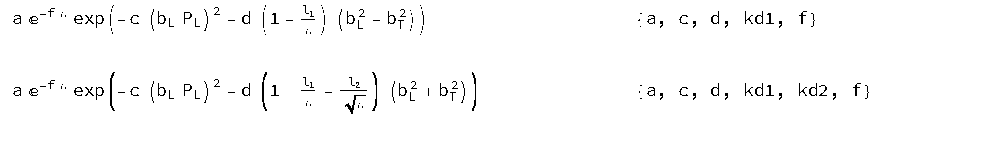
\includegraphics[width=\linewidth,height=.72\textheight,keepaspectratio]{fitting/fit_list_gaussian_c_d_etas__block3_part1.pdf}
\par\small $P_L=-1$, $|\vect b|\ge3a$, $6\le\eta\le10$. Original thesis table, enlarged without omitted rows.

\figsrc{Thesis: plots; fit\_list\_gaussian\_c\_d\_etas}
\end{frame}

\begin{frame}{Gaussian candidates --- block 3, parameters and diagnostics}
\centering
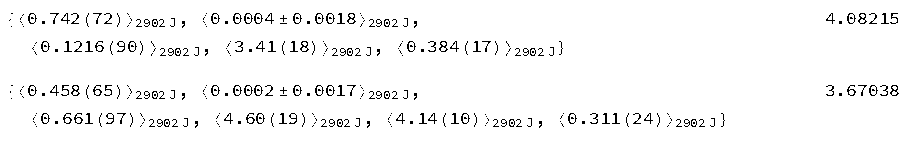
\includegraphics[width=\linewidth,height=.72\textheight,keepaspectratio]{fitting/fit_list_gaussian_c_d_etas__block3_part2.pdf}
\par\small $P_L=-1$, $|\vect b|\ge3a$, $6\le\eta\le10$. Original thesis table, enlarged without omitted rows.

\figsrc{Thesis: plots; fit\_list\_gaussian\_c\_d\_etas}
\end{frame}

\begin{frame}{Gaussian candidates --- block 4, models}
\centering
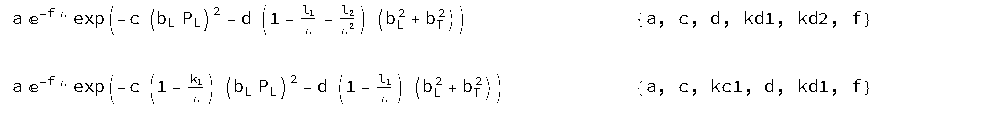
\includegraphics[width=\linewidth,height=.72\textheight,keepaspectratio]{fitting/fit_list_gaussian_c_d_etas__block4_part1.pdf}
\par\small $P_L=-1$, $|\vect b|\ge3a$, $6\le\eta\le10$. Original thesis table, enlarged without omitted rows.

\figsrc{Thesis: plots; fit\_list\_gaussian\_c\_d\_etas}
\end{frame}

\begin{frame}{Gaussian candidates --- block 4, parameters and diagnostics}
\centering
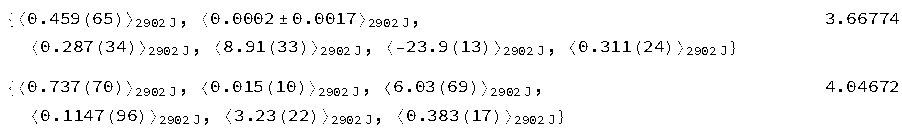
\includegraphics[width=\linewidth,height=.72\textheight,keepaspectratio]{fitting/fit_list_gaussian_c_d_etas__block4_part2.pdf}
\par\small $P_L=-1$, $|\vect b|\ge3a$, $6\le\eta\le10$. Original thesis table, enlarged without omitted rows.

\figsrc{Thesis: plots; fit\_list\_gaussian\_c\_d\_etas}
\end{frame}

\begin{frame}{Gaussian candidates --- block 5, models}
\centering
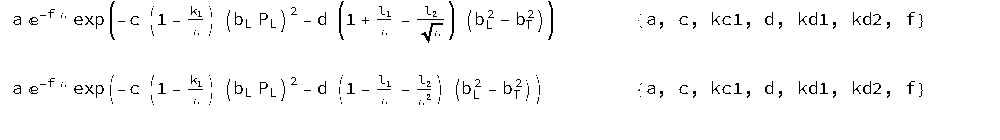
\includegraphics[width=\linewidth,height=.72\textheight,keepaspectratio]{fitting/fit_list_gaussian_c_d_etas__block5_part1.pdf}
\par\small $P_L=-1$, $|\vect b|\ge3a$, $6\le\eta\le10$. Original thesis table, enlarged without omitted rows.

\figsrc{Thesis: plots; fit\_list\_gaussian\_c\_d\_etas}
\end{frame}

\begin{frame}{Gaussian candidates --- block 5, parameters and diagnostics}
\centering
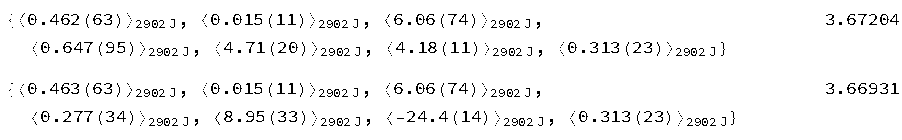
\includegraphics[width=\linewidth,height=.72\textheight,keepaspectratio]{fitting/fit_list_gaussian_c_d_etas__block5_part2.pdf}
\par\small $P_L=-1$, $|\vect b|\ge3a$, $6\le\eta\le10$. Original thesis table, enlarged without omitted rows.

\figsrc{Thesis: plots; fit\_list\_gaussian\_c\_d\_etas}
\end{frame}

\begin{frame}{Gaussian candidates --- block 6, models}
\centering
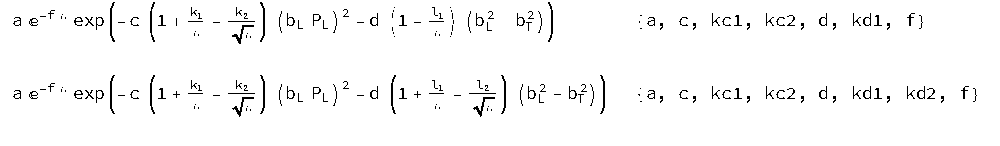
\includegraphics[width=\linewidth,height=.72\textheight,keepaspectratio]{fitting/fit_list_gaussian_c_d_etas__block6_part1.pdf}
\par\small $P_L=-1$, $|\vect b|\ge3a$, $6\le\eta\le10$. Original thesis table, enlarged without omitted rows.

\figsrc{Thesis: plots; fit\_list\_gaussian\_c\_d\_etas}
\end{frame}

\begin{frame}{Gaussian candidates --- block 6, parameters and diagnostics}
\centering
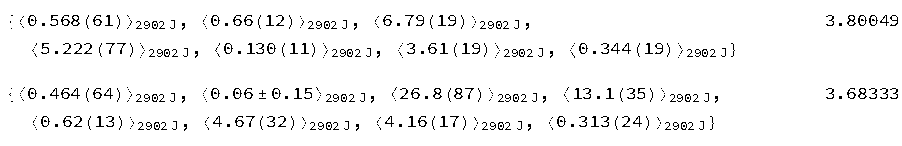
\includegraphics[width=\linewidth,height=.72\textheight,keepaspectratio]{fitting/fit_list_gaussian_c_d_etas__block6_part2.pdf}
\par\small $P_L=-1$, $|\vect b|\ge3a$, $6\le\eta\le10$. Original thesis table, enlarged without omitted rows.

\figsrc{Thesis: plots; fit\_list\_gaussian\_c\_d\_etas}
\end{frame}

\begin{frame}{Gaussian candidates --- block 7, models}
\centering
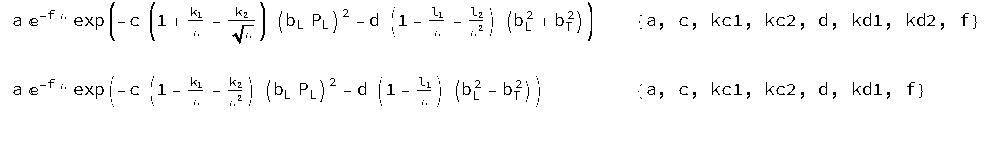
\includegraphics[width=\linewidth,height=.72\textheight,keepaspectratio]{fitting/fit_list_gaussian_c_d_etas__block7_part1.pdf}
\par\small $P_L=-1$, $|\vect b|\ge3a$, $6\le\eta\le10$. Original thesis table, enlarged without omitted rows.

\figsrc{Thesis: plots; fit\_list\_gaussian\_c\_d\_etas}
\end{frame}

\begin{frame}{Gaussian candidates --- block 7, parameters and diagnostics}
\centering
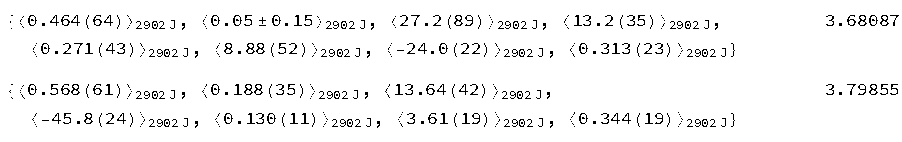
\includegraphics[width=\linewidth,height=.72\textheight,keepaspectratio]{fitting/fit_list_gaussian_c_d_etas__block7_part2.pdf}
\par\small $P_L=-1$, $|\vect b|\ge3a$, $6\le\eta\le10$. Original thesis table, enlarged without omitted rows.

\figsrc{Thesis: plots; fit\_list\_gaussian\_c\_d\_etas}
\end{frame}

\begin{frame}{Gaussian candidates --- block 8, models}
\centering
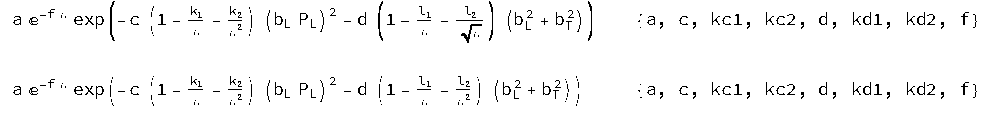
\includegraphics[width=\linewidth,height=.72\textheight,keepaspectratio]{fitting/fit_list_gaussian_c_d_etas__block8_part1.pdf}
\par\small $P_L=-1$, $|\vect b|\ge3a$, $6\le\eta\le10$. Original thesis table, enlarged without omitted rows.

\figsrc{Thesis: plots; fit\_list\_gaussian\_c\_d\_etas}
\end{frame}

\begin{frame}{Gaussian candidates --- block 8, parameters and diagnostics}
\centering
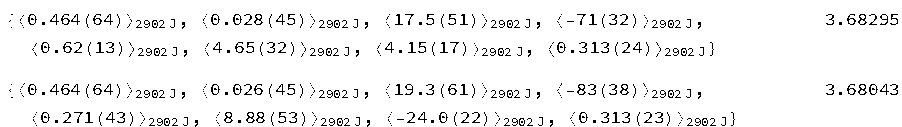
\includegraphics[width=\linewidth,height=.72\textheight,keepaspectratio]{fitting/fit_list_gaussian_c_d_etas__block8_part2.pdf}
\par\small $P_L=-1$, $|\vect b|\ge3a$, $6\le\eta\le10$. Original thesis table, enlarged without omitted rows.

\figsrc{Thesis: plots; fit\_list\_gaussian\_c\_d\_etas}
\end{frame}

\begin{frame}{Power-law candidates: finite-width continuation}

\[F(\nu,b^2,\eta)=a e^{-f\eta}\left[1+c(\eta)\frac{\nu^2}{P_L^2}+db^2\right]^{-j}.\]
\begin{itemize}
\item First compare a constant $c$, inverse powers of $\eta$, logarithmic corrections, and an exponential correction.
\item Then compare forms giving wider Fourier profiles. Each original row includes its full equation, parameters, $\chi^2/\mathrm{dof}$, AIC, and Fourier plot.
\item AIC compares likelihood fit quality and parameter count on the same data: $\mathrm{AIC}=2k-2\log\widehat{\mathcal L}$; for fixed Gaussian covariance this is $\chi^2+2k$ up to a common constant.
\end{itemize}
\figsrc{Thesis: Fitting Methodologies and Stability Analysis}
\end{frame}

\begin{frame}{Power-law candidate diagnostics --- block 1, models}
\centering
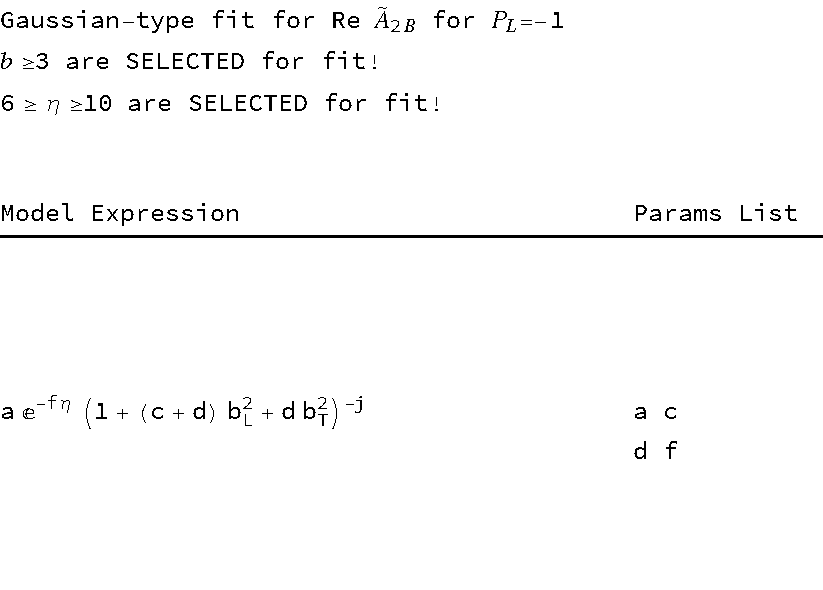
\includegraphics[width=\linewidth,height=.72\textheight,keepaspectratio]{fitting/A2BfitFT_eta_Asymptotic_P1__block1_part1.pdf}
\par\small $P_L=-1$, $|\vect b|\ge3a$, $6\le\eta\le10$. Original thesis table, enlarged without omitted rows.

\figsrc{Thesis: PowerLaw\_etaAsymptotic; A2BfitFT\_eta\_Asymptotic\_P1}
\end{frame}

\begin{frame}{Power-law candidate diagnostics --- block 1, parameters and diagnostics}
\centering
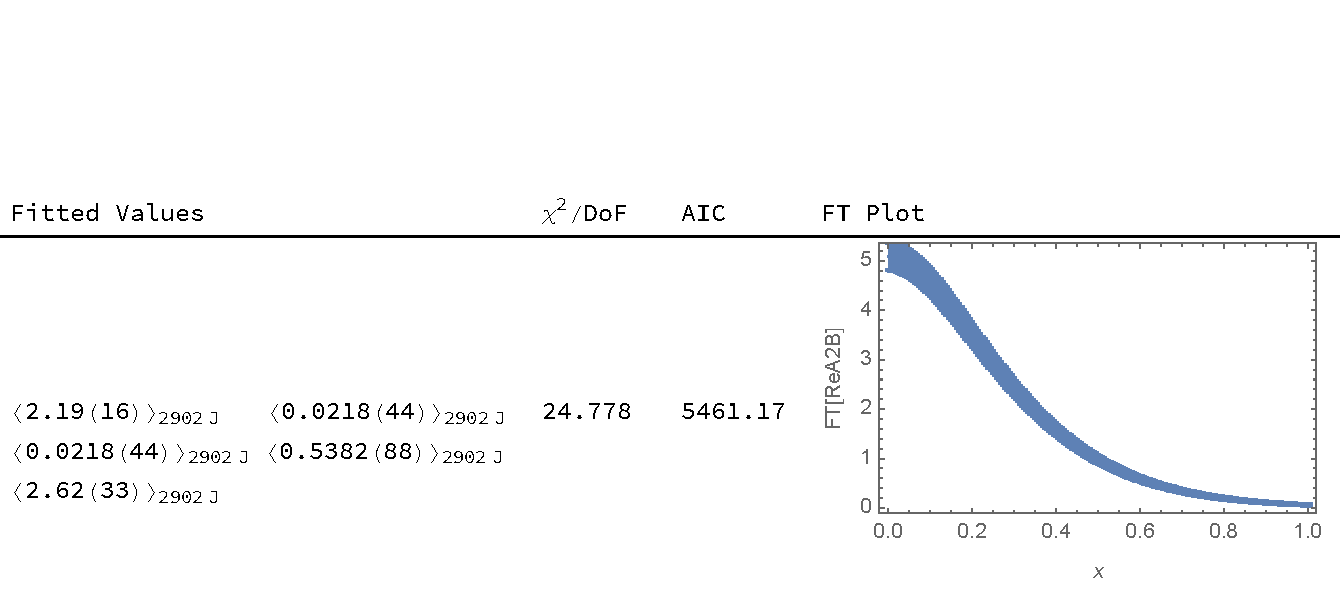
\includegraphics[width=\linewidth,height=.72\textheight,keepaspectratio]{fitting/A2BfitFT_eta_Asymptotic_P1__block1_part2.pdf}
\par\small $P_L=-1$, $|\vect b|\ge3a$, $6\le\eta\le10$. Original thesis table, enlarged without omitted rows.

\figsrc{Thesis: PowerLaw\_etaAsymptotic; A2BfitFT\_eta\_Asymptotic\_P1}
\end{frame}

\begin{frame}{Power-law candidate diagnostics --- block 2, models}
\centering
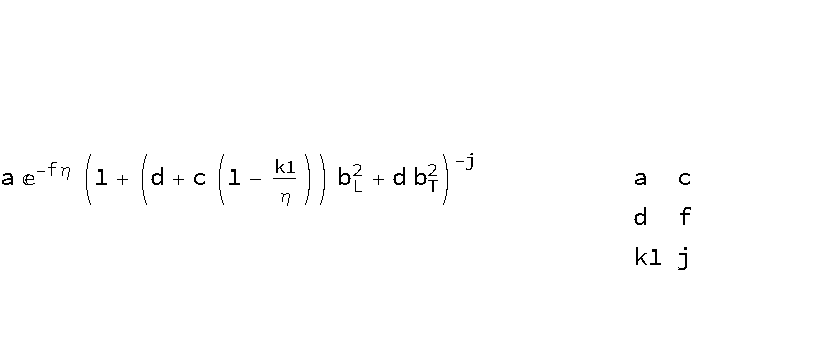
\includegraphics[width=\linewidth,height=.72\textheight,keepaspectratio]{fitting/A2BfitFT_eta_Asymptotic_P1__block2_part1.pdf}
\par\small $P_L=-1$, $|\vect b|\ge3a$, $6\le\eta\le10$. Original thesis table, enlarged without omitted rows.

\figsrc{Thesis: PowerLaw\_etaAsymptotic; A2BfitFT\_eta\_Asymptotic\_P1}
\end{frame}

\begin{frame}{Power-law candidate diagnostics --- block 2, parameters and diagnostics}
\centering
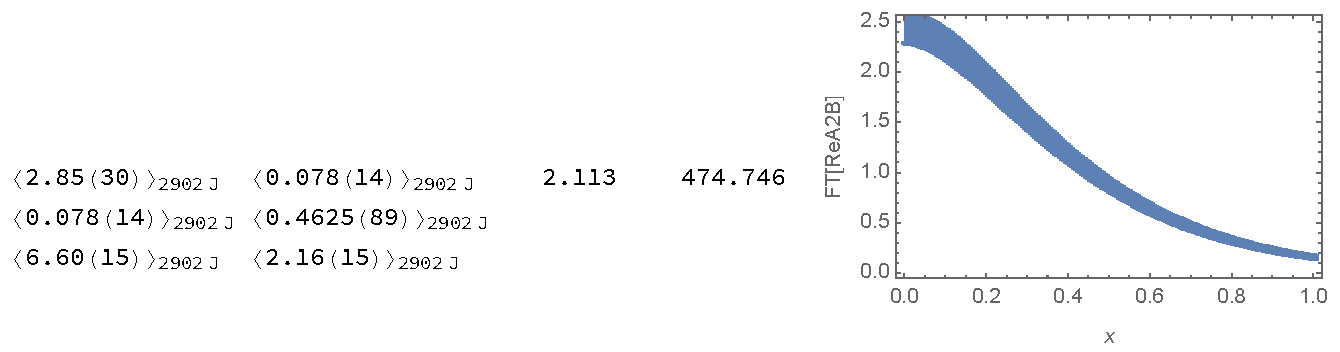
\includegraphics[width=\linewidth,height=.72\textheight,keepaspectratio]{fitting/A2BfitFT_eta_Asymptotic_P1__block2_part2.pdf}
\par\small $P_L=-1$, $|\vect b|\ge3a$, $6\le\eta\le10$. Original thesis table, enlarged without omitted rows.

\figsrc{Thesis: PowerLaw\_etaAsymptotic; A2BfitFT\_eta\_Asymptotic\_P1}
\end{frame}

\begin{frame}{Power-law candidate diagnostics --- block 3, models}
\centering
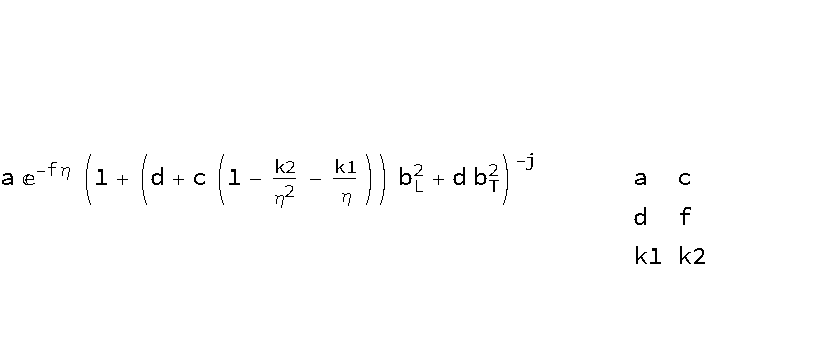
\includegraphics[width=\linewidth,height=.72\textheight,keepaspectratio]{fitting/A2BfitFT_eta_Asymptotic_P1__block3_part1.pdf}
\par\small $P_L=-1$, $|\vect b|\ge3a$, $6\le\eta\le10$. Original thesis table, enlarged without omitted rows.

\figsrc{Thesis: PowerLaw\_etaAsymptotic; A2BfitFT\_eta\_Asymptotic\_P1}
\end{frame}

\begin{frame}{Power-law candidate diagnostics --- block 3, parameters and diagnostics}
\centering
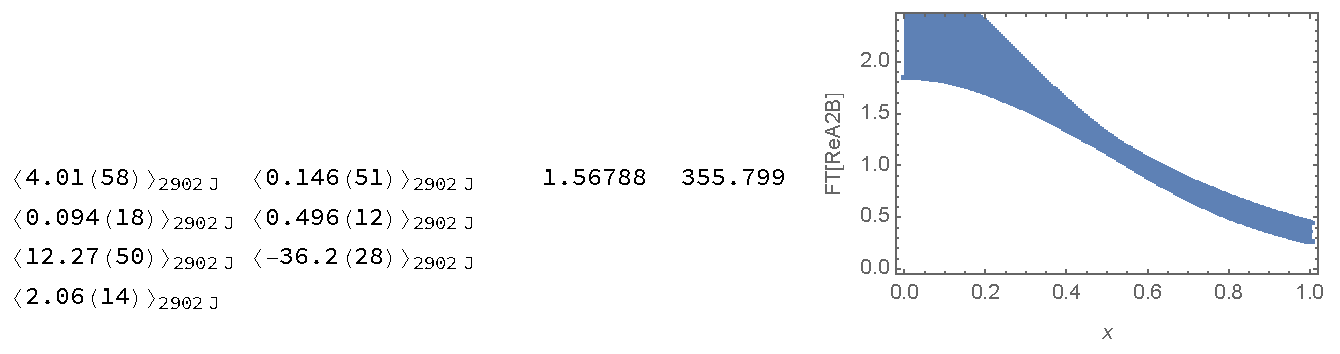
\includegraphics[width=\linewidth,height=.72\textheight,keepaspectratio]{fitting/A2BfitFT_eta_Asymptotic_P1__block3_part2.pdf}
\par\small $P_L=-1$, $|\vect b|\ge3a$, $6\le\eta\le10$. Original thesis table, enlarged without omitted rows.

\figsrc{Thesis: PowerLaw\_etaAsymptotic; A2BfitFT\_eta\_Asymptotic\_P1}
\end{frame}

\begin{frame}{Power-law candidate diagnostics --- block 4, models}
\centering
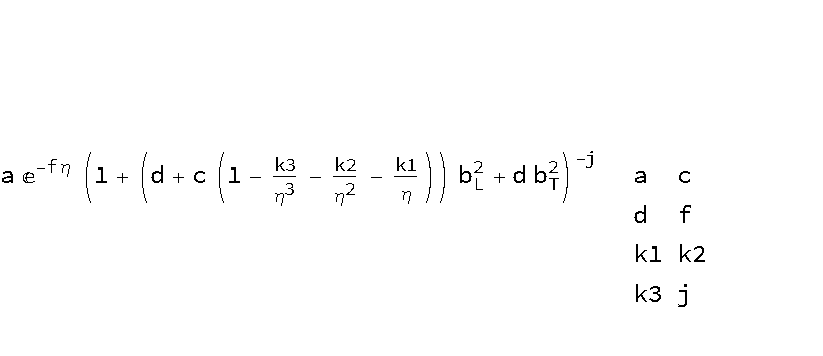
\includegraphics[width=\linewidth,height=.72\textheight,keepaspectratio]{fitting/A2BfitFT_eta_Asymptotic_P1__block4_part1.pdf}
\par\small $P_L=-1$, $|\vect b|\ge3a$, $6\le\eta\le10$. Original thesis table, enlarged without omitted rows.

\figsrc{Thesis: PowerLaw\_etaAsymptotic; A2BfitFT\_eta\_Asymptotic\_P1}
\end{frame}

\begin{frame}{Power-law candidate diagnostics --- block 4, parameters and diagnostics}
\centering
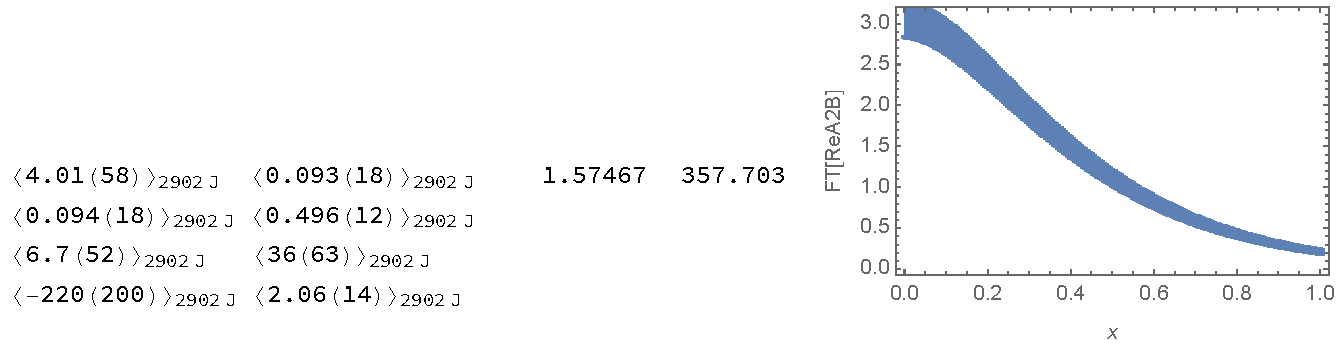
\includegraphics[width=\linewidth,height=.72\textheight,keepaspectratio]{fitting/A2BfitFT_eta_Asymptotic_P1__block4_part2.pdf}
\par\small $P_L=-1$, $|\vect b|\ge3a$, $6\le\eta\le10$. Original thesis table, enlarged without omitted rows.

\figsrc{Thesis: PowerLaw\_etaAsymptotic; A2BfitFT\_eta\_Asymptotic\_P1}
\end{frame}

\begin{frame}{Power-law candidate diagnostics --- block 5, models}
\centering
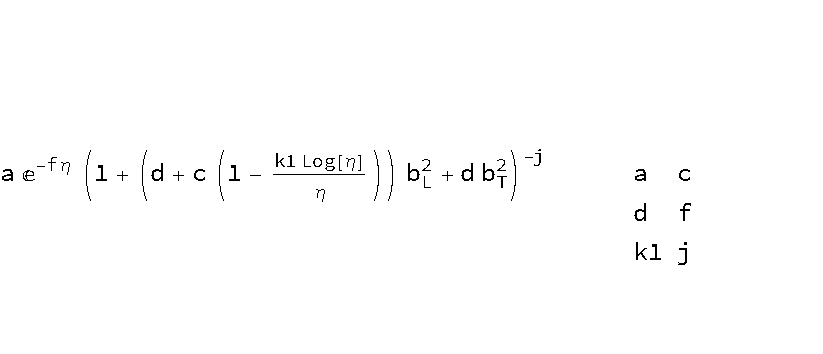
\includegraphics[width=\linewidth,height=.72\textheight,keepaspectratio]{fitting/A2BfitFT_eta_Asymptotic_P1__block5_part1.pdf}
\par\small $P_L=-1$, $|\vect b|\ge3a$, $6\le\eta\le10$. Original thesis table, enlarged without omitted rows.

\figsrc{Thesis: PowerLaw\_etaAsymptotic; A2BfitFT\_eta\_Asymptotic\_P1}
\end{frame}

\begin{frame}{Power-law candidate diagnostics --- block 5, parameters and diagnostics}
\centering
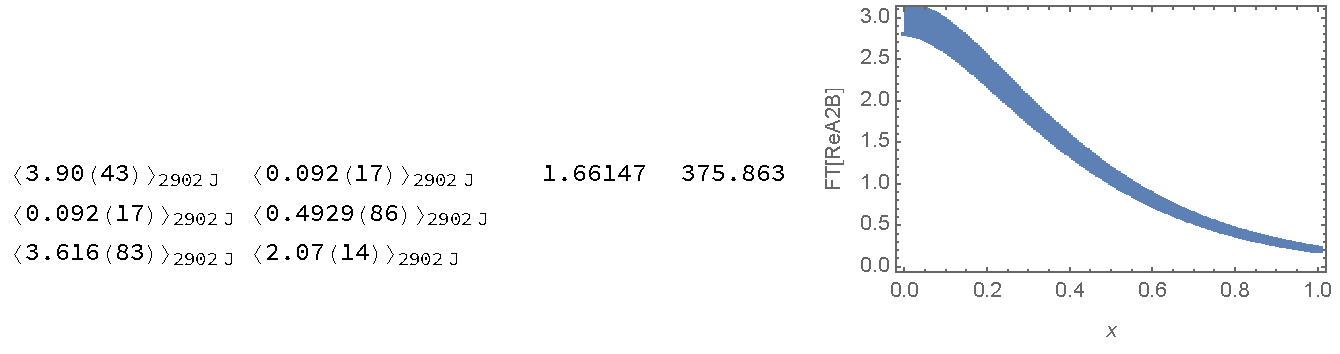
\includegraphics[width=\linewidth,height=.72\textheight,keepaspectratio]{fitting/A2BfitFT_eta_Asymptotic_P1__block5_part2.pdf}
\par\small $P_L=-1$, $|\vect b|\ge3a$, $6\le\eta\le10$. Original thesis table, enlarged without omitted rows.

\figsrc{Thesis: PowerLaw\_etaAsymptotic; A2BfitFT\_eta\_Asymptotic\_P1}
\end{frame}

\begin{frame}{Power-law candidate diagnostics --- block 6, models}
\centering
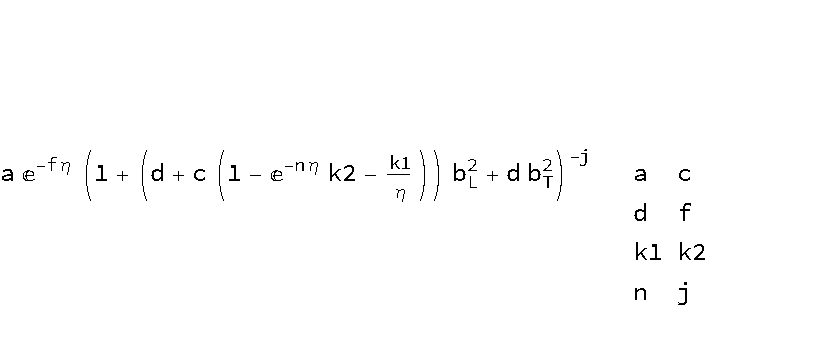
\includegraphics[width=\linewidth,height=.72\textheight,keepaspectratio]{fitting/A2BfitFT_eta_Asymptotic_P1__block6_part1.pdf}
\par\small $P_L=-1$, $|\vect b|\ge3a$, $6\le\eta\le10$. Original thesis table, enlarged without omitted rows.

\figsrc{Thesis: PowerLaw\_etaAsymptotic; A2BfitFT\_eta\_Asymptotic\_P1}
\end{frame}

\begin{frame}{Power-law candidate diagnostics --- block 6, parameters and diagnostics}
\centering
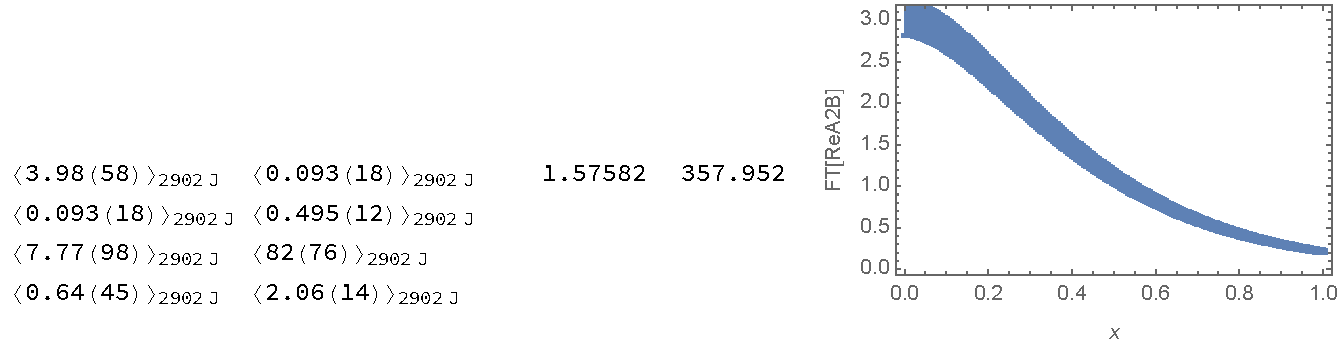
\includegraphics[width=\linewidth,height=.72\textheight,keepaspectratio]{fitting/A2BfitFT_eta_Asymptotic_P1__block6_part2.pdf}
\par\small $P_L=-1$, $|\vect b|\ge3a$, $6\le\eta\le10$. Original thesis table, enlarged without omitted rows.

\figsrc{Thesis: PowerLaw\_etaAsymptotic; A2BfitFT\_eta\_Asymptotic\_P1}
\end{frame}

\begin{frame}{Wider Fourier-profile candidate diagnostics --- block 1, models}
\centering
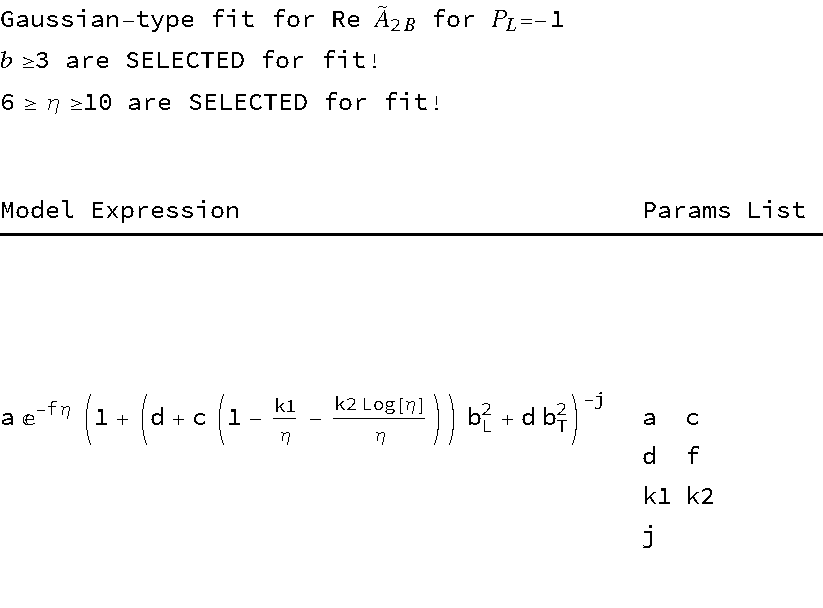
\includegraphics[width=\linewidth,height=.72\textheight,keepaspectratio]{fitting/A2Bfit_widerFT_eta_Asymptotic_P1__block1_part1.pdf}
\par\small $P_L=-1$, $|\vect b|\ge3a$, $6\le\eta\le10$. Original thesis table, enlarged without omitted rows.

\figsrc{Thesis: PowerLaw\_etaAsymptotic; A2Bfit\_widerFT\_eta\_Asymptotic\_P1}
\end{frame}

\begin{frame}{Wider Fourier-profile candidate diagnostics --- block 1, parameters and diagnostics}
\centering
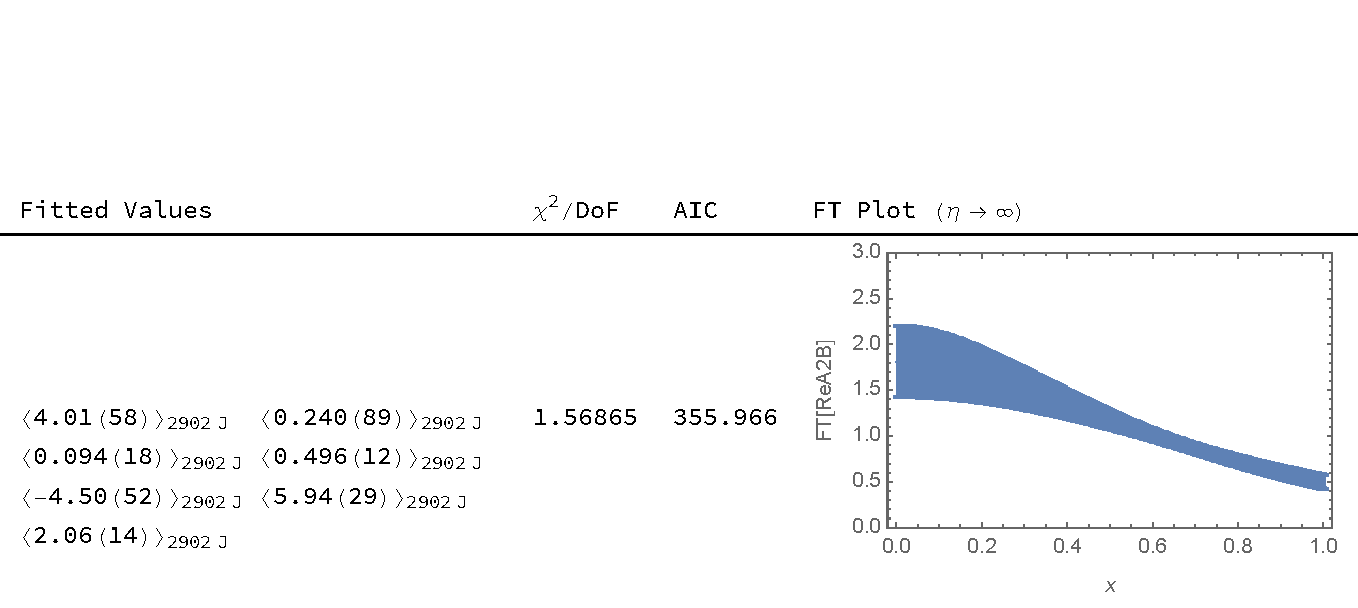
\includegraphics[width=\linewidth,height=.72\textheight,keepaspectratio]{fitting/A2Bfit_widerFT_eta_Asymptotic_P1__block1_part2.pdf}
\par\small $P_L=-1$, $|\vect b|\ge3a$, $6\le\eta\le10$. Original thesis table, enlarged without omitted rows.

\figsrc{Thesis: PowerLaw\_etaAsymptotic; A2Bfit\_widerFT\_eta\_Asymptotic\_P1}
\end{frame}

\begin{frame}{Wider Fourier-profile candidate diagnostics --- block 2, models}
\centering
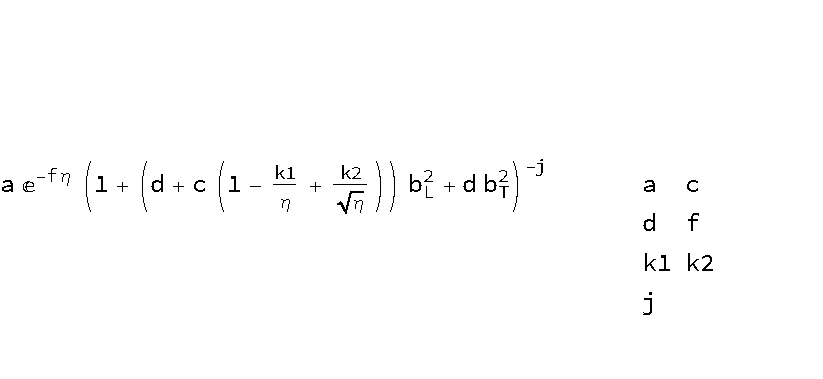
\includegraphics[width=\linewidth,height=.72\textheight,keepaspectratio]{fitting/A2Bfit_widerFT_eta_Asymptotic_P1__block2_part1.pdf}
\par\small $P_L=-1$, $|\vect b|\ge3a$, $6\le\eta\le10$. Original thesis table, enlarged without omitted rows.

\figsrc{Thesis: PowerLaw\_etaAsymptotic; A2Bfit\_widerFT\_eta\_Asymptotic\_P1}
\end{frame}

\begin{frame}{Wider Fourier-profile candidate diagnostics --- block 2, parameters and diagnostics}
\centering
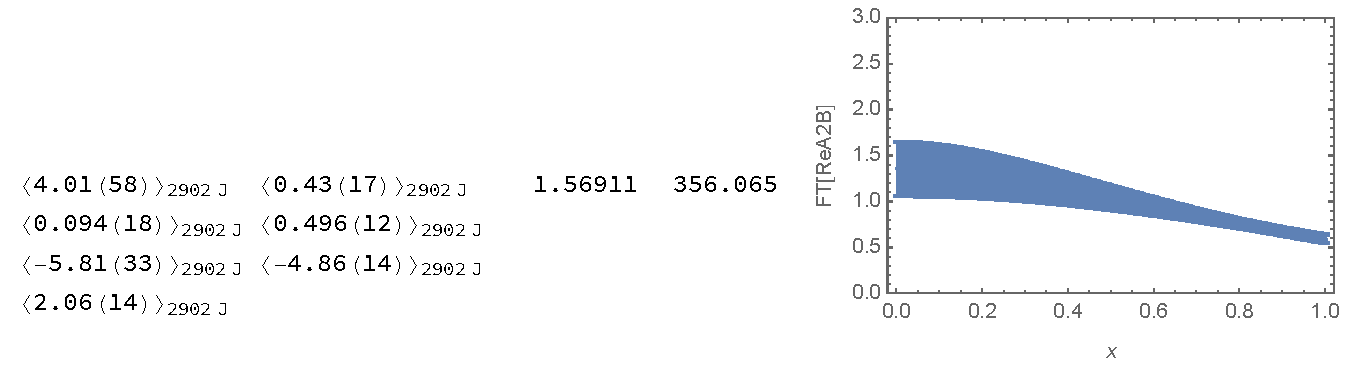
\includegraphics[width=\linewidth,height=.72\textheight,keepaspectratio]{fitting/A2Bfit_widerFT_eta_Asymptotic_P1__block2_part2.pdf}
\par\small $P_L=-1$, $|\vect b|\ge3a$, $6\le\eta\le10$. Original thesis table, enlarged without omitted rows.

\figsrc{Thesis: PowerLaw\_etaAsymptotic; A2Bfit\_widerFT\_eta\_Asymptotic\_P1}
\end{frame}

\begin{frame}{Wider Fourier-profile candidate diagnostics --- block 3, models}
\centering
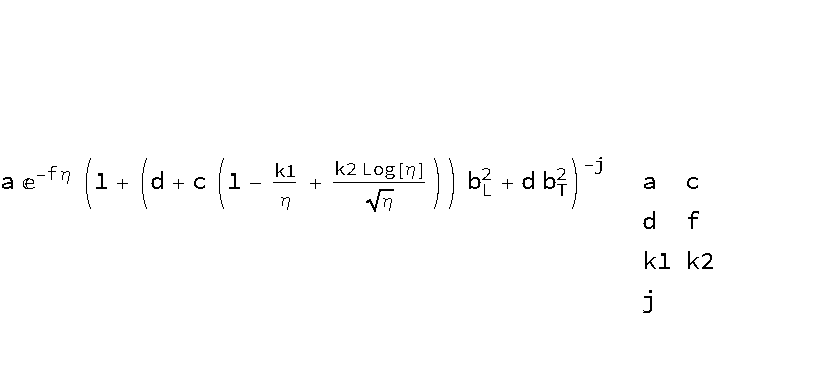
\includegraphics[width=\linewidth,height=.72\textheight,keepaspectratio]{fitting/A2Bfit_widerFT_eta_Asymptotic_P1__block3_part1.pdf}
\par\small $P_L=-1$, $|\vect b|\ge3a$, $6\le\eta\le10$. Original thesis table, enlarged without omitted rows.

\figsrc{Thesis: PowerLaw\_etaAsymptotic; A2Bfit\_widerFT\_eta\_Asymptotic\_P1}
\end{frame}

\begin{frame}{Wider Fourier-profile candidate diagnostics --- block 3, parameters and diagnostics}
\centering
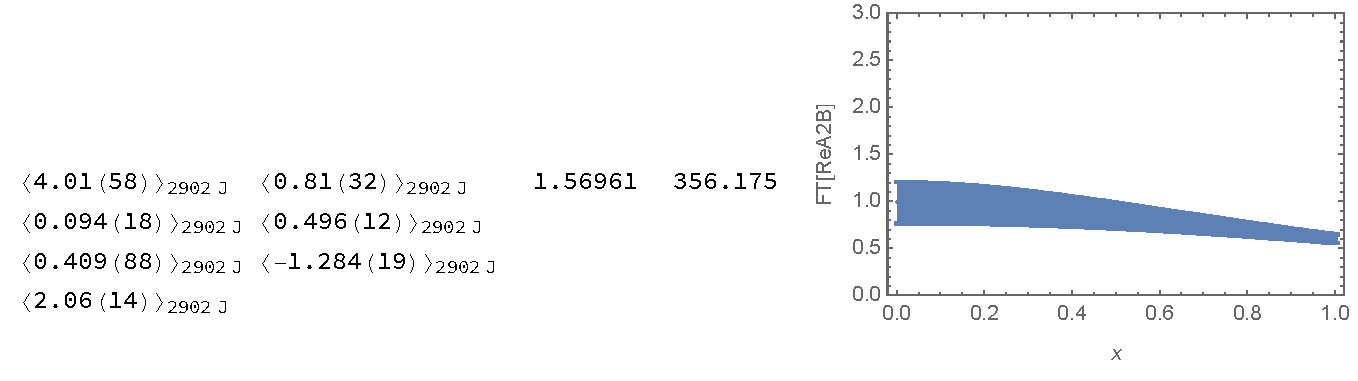
\includegraphics[width=\linewidth,height=.72\textheight,keepaspectratio]{fitting/A2Bfit_widerFT_eta_Asymptotic_P1__block3_part2.pdf}
\par\small $P_L=-1$, $|\vect b|\ge3a$, $6\le\eta\le10$. Original thesis table, enlarged without omitted rows.

\figsrc{Thesis: PowerLaw\_etaAsymptotic; A2Bfit\_widerFT\_eta\_Asymptotic\_P1}
\end{frame}

\begin{frame}{Wider Fourier-profile candidate diagnostics --- block 4, models}
\centering
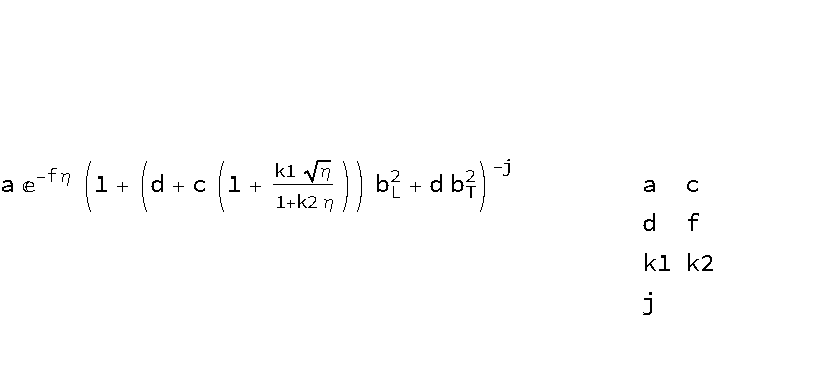
\includegraphics[width=\linewidth,height=.72\textheight,keepaspectratio]{fitting/A2Bfit_widerFT_eta_Asymptotic_P1__block4_part1.pdf}
\par\small $P_L=-1$, $|\vect b|\ge3a$, $6\le\eta\le10$. Original thesis table, enlarged without omitted rows.

\figsrc{Thesis: PowerLaw\_etaAsymptotic; A2Bfit\_widerFT\_eta\_Asymptotic\_P1}
\end{frame}

\begin{frame}{Wider Fourier-profile candidate diagnostics --- block 4, parameters and diagnostics}
\centering
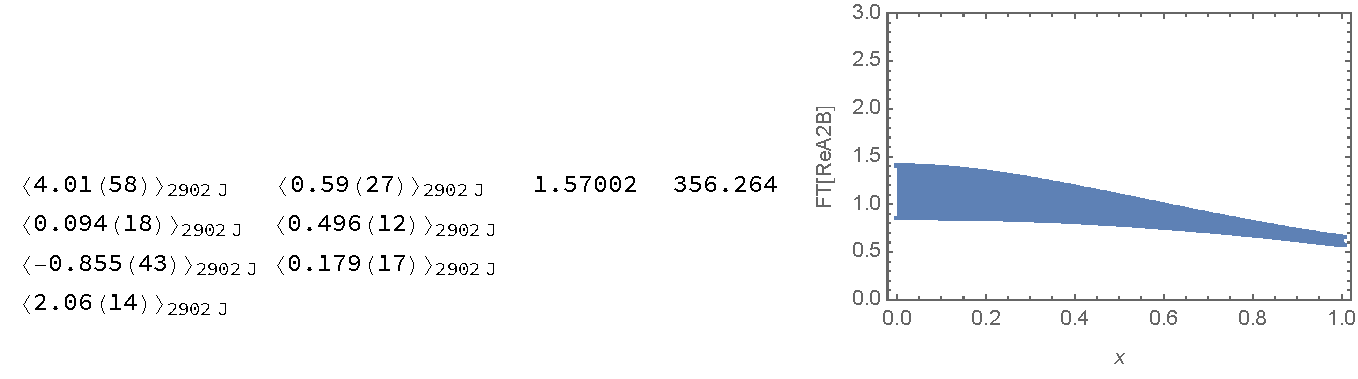
\includegraphics[width=\linewidth,height=.72\textheight,keepaspectratio]{fitting/A2Bfit_widerFT_eta_Asymptotic_P1__block4_part2.pdf}
\par\small $P_L=-1$, $|\vect b|\ge3a$, $6\le\eta\le10$. Original thesis table, enlarged without omitted rows.

\figsrc{Thesis: PowerLaw\_etaAsymptotic; A2Bfit\_widerFT\_eta\_Asymptotic\_P1}
\end{frame}

\begin{frame}{All ten asymptotic width candidates (1/2)}
\begin{align*}c_{1}(\eta)&=c(1-k_1/\eta)\\[2mm]
c_{2}(\eta)&=c(1-k_1/\eta-k_2/\eta^2)\\[2mm]
c_{3}(\eta)&=c(1-k_1/\eta-k_2/\eta^2-k_3/\eta^3)\\[2mm]
c_{4}(\eta)&=c(1-k_1\log\eta/\eta)\\[2mm]
c_{5}(\eta)&=c(1-k_1/\eta-k_2\log\eta/\eta)\\[2mm]\end{align*}
\figsrc{Thesis: Fitting Methodologies and Stability Analysis}
\end{frame}

\begin{frame}{All ten asymptotic width candidates (2/2)}
\begin{align*}c_{6}(\eta)&=c(1-k_1/\eta+k_2/\sqrt\eta)\\[2mm]
c_{7}(\eta)&=c(1-k_1/\eta+k_2\log\eta/\sqrt\eta)\\[2mm]
c_{8}(\eta)&=c(1+k_1\sqrt\eta/(1+k_2\eta))\\[2mm]
c_{9}(\eta)&=c(1-k_1/\eta^{0.2}+k_2/\eta^{0.8})\\[2mm]
c_{10}(\eta)&=c(1-k_1/\eta^{0.3}+k_2/\eta^{0.7})\\[2mm]\end{align*}
\figsrc{Thesis: Fitting Methodologies and Stability Analysis}
\end{frame}

\begin{frame}{Fixed-$\eta$ fits: $\tAmp_{2B}^{\mathrm{Re}}$}
\centering
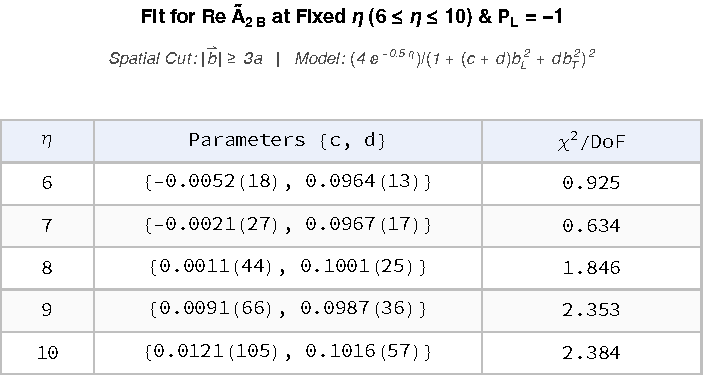
\includegraphics[width=\linewidth,height=.70\textheight,keepaspectratio]{fitting/LorentzianFixedA_P-1_b3.pdf}
\par\small Fix $a=4$, $j=2$, $f=0.5$ to isolate $c(\eta)$ and $d(\eta)$.

\figsrc{Thesis: Gaussian\_type\_fit\_Real\_A2B; LorentzianFixedA\_P-1\_b3}
\end{frame}

\begin{frame}{$c_1$ through $c_{10}$ against the extracted widths}
\centering
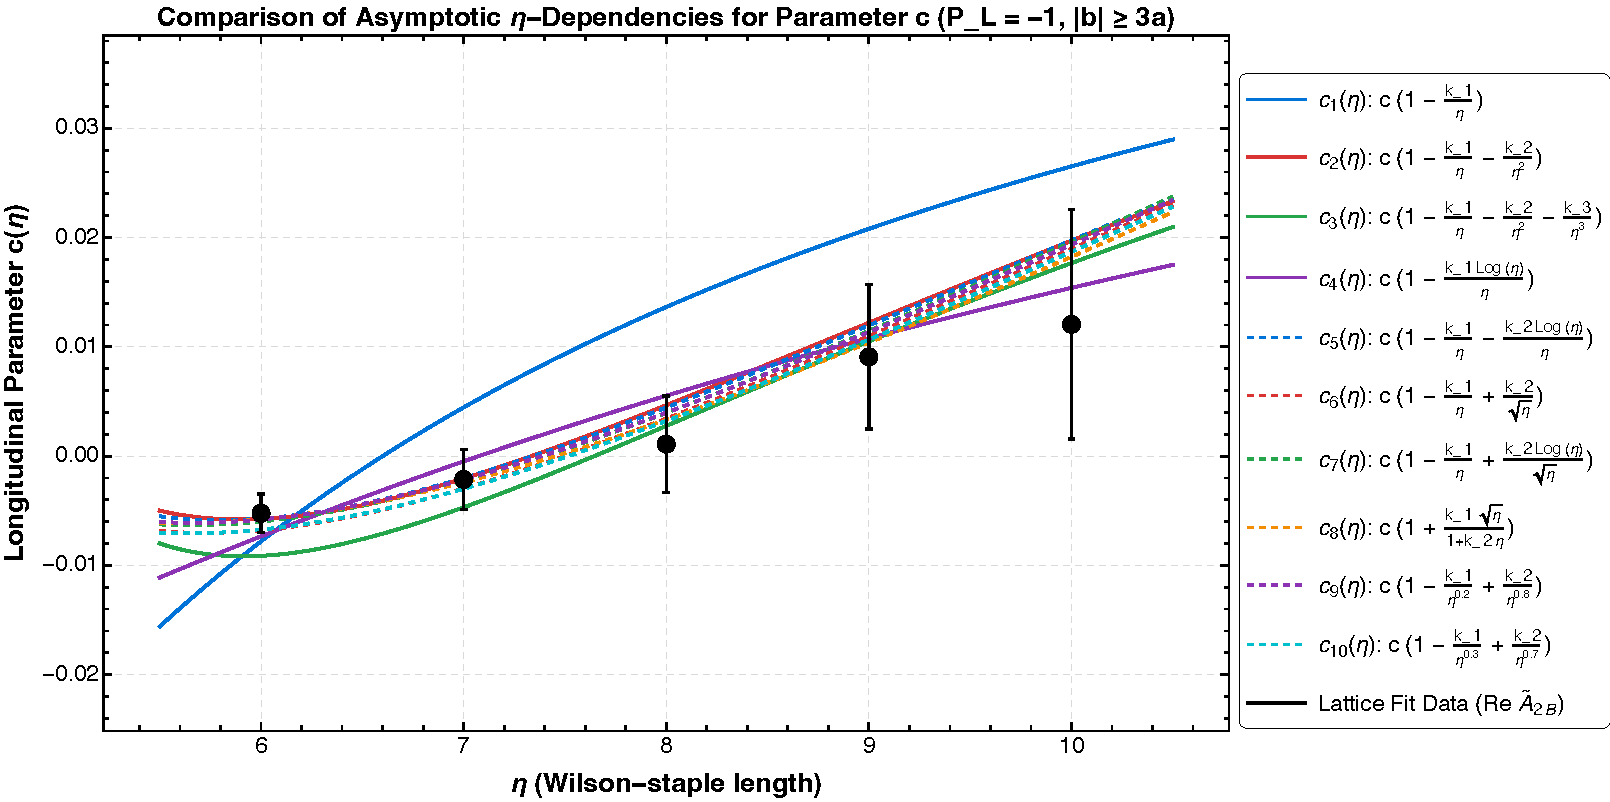
\includegraphics[width=\linewidth,height=.70\textheight,keepaspectratio]{fitting/A2B_c_eta_AllAsymptoticModels_P1.pdf}
\par\small Several forms describe the measured staple range similarly.

\figsrc{Thesis: PowerLaw\_etaAsymptotic; A2B\_c\_eta\_AllAsymptoticModels\_P1}
\end{frame}

\begin{frame}{Transverse width: $\tAmp_{2B}^{\mathrm{Re}}$}
\centering
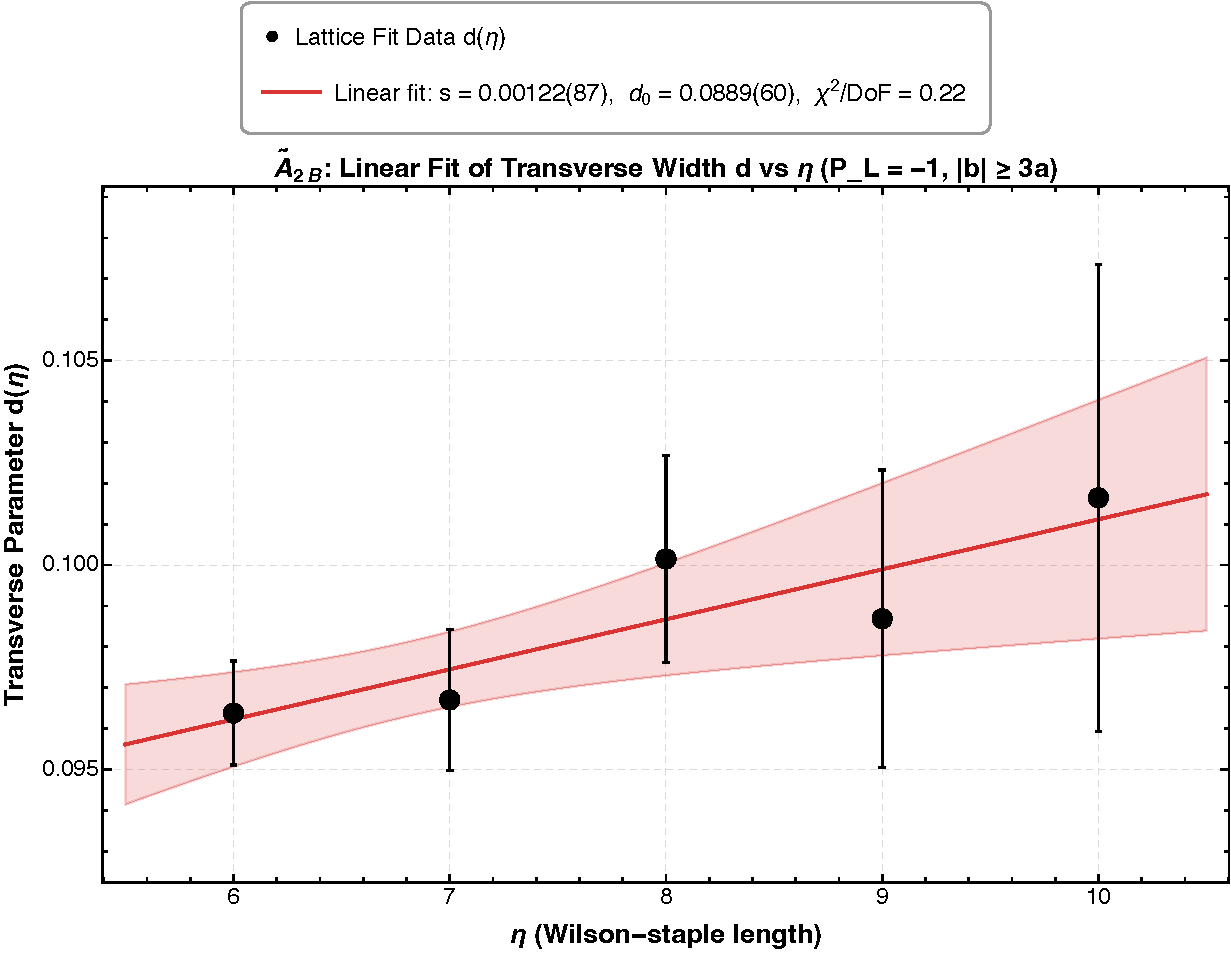
\includegraphics[width=\linewidth,height=.70\textheight,keepaspectratio]{fitting/A2B_d_eta_Independence_P1.pdf}
\par\small $s=0.00122(87)$, $d_0=0.0889(60)$, $\chi^2/\mathrm{dof}=0.22$: keep $d$ constant.

\figsrc{Thesis: PowerLaw\_etaAsymptotic; A2B\_d\_eta\_Independence\_P1}
\end{frame}

\begin{frame}{Fixed-$\eta$ fits: $\tAmp_{12B}^{\mathrm{Re}}$}
\centering
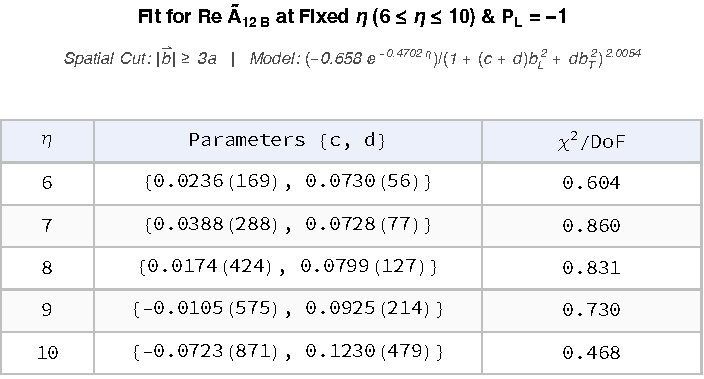
\includegraphics[width=\linewidth,height=.70\textheight,keepaspectratio]{fitting/LorentzianFixed_ReA12B_P-1_b3.pdf}
\par\small All five staple slices and their fit statistics.

\figsrc{Thesis: Gaussian\_type\_fit\_Real\_A2B; LorentzianFixed\_ReA12B\_P-1\_b3}
\end{frame}

\begin{frame}{Fixed-$\eta$ fits: $\tAmp_{2B}^{\mathrm{Im}}$}
\centering
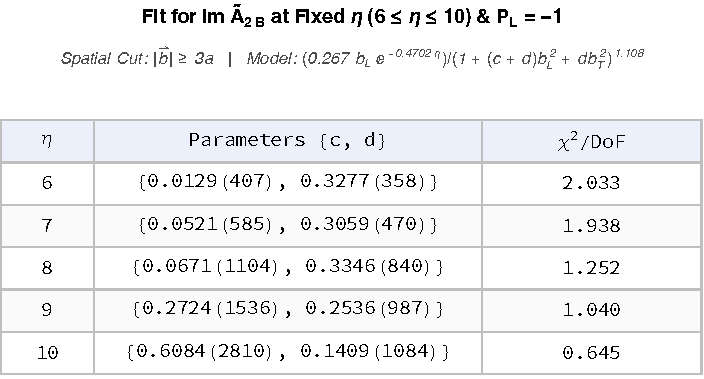
\includegraphics[width=\linewidth,height=.70\textheight,keepaspectratio]{fitting/LorentzianFixed_ImA2B_P-1_b3.pdf}
\par\small All five staple slices and their fit statistics.

\figsrc{Thesis: Gaussian\_type\_fit\_Real\_A2B; LorentzianFixed\_ImA2B\_P-1\_b3}
\end{frame}

\begin{frame}{Staple dependence of $c$: $\tAmp_{12B}^{\mathrm{Re}}$}
\centering
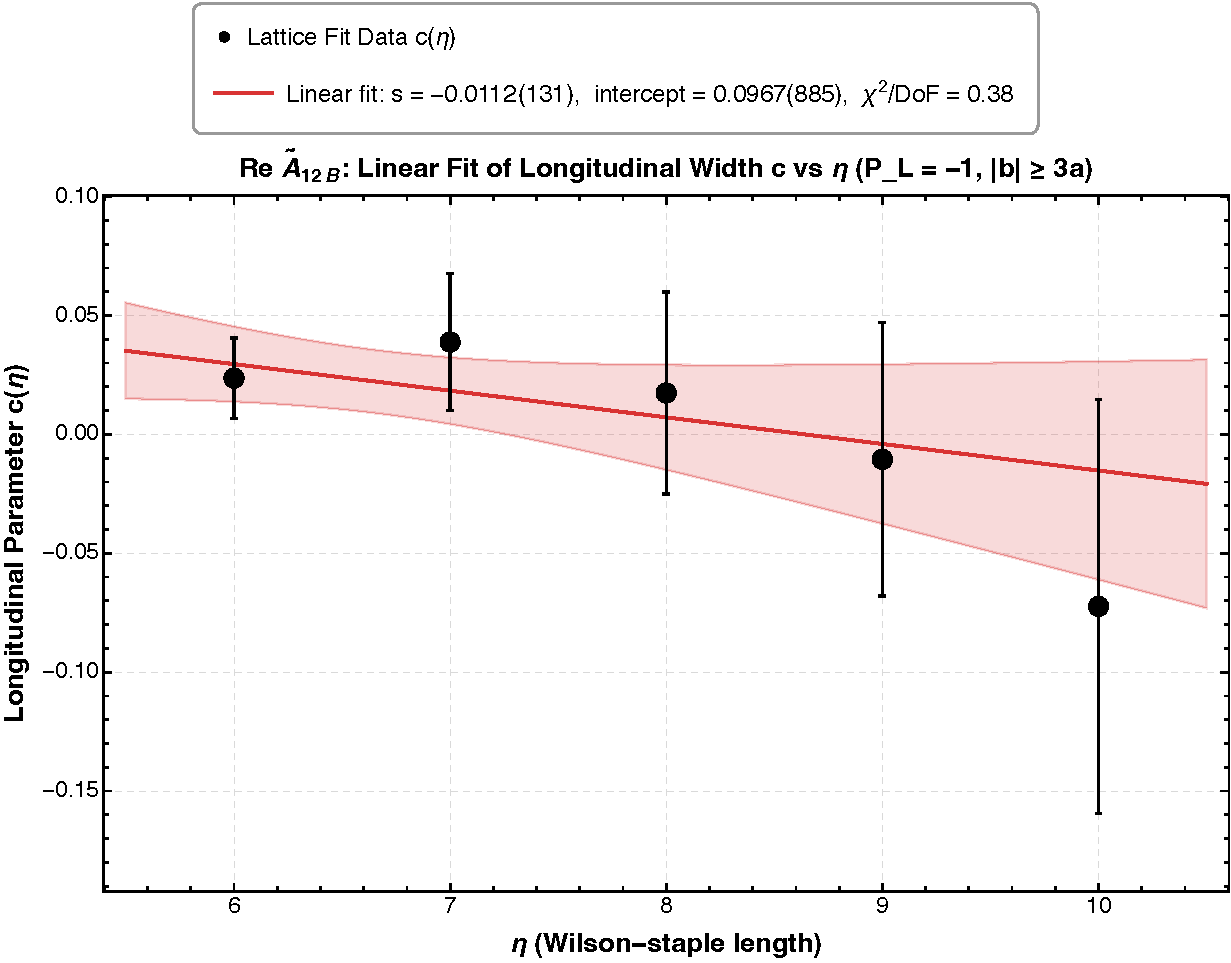
\includegraphics[width=\linewidth,height=.70\textheight,keepaspectratio]{fitting/ReA12B_c_eta_Independence_P1.pdf}
\par\small Slopes: $s_c=-0.0112(131)$, $s_d=0.0052(48)$; both compatible with zero.

\figsrc{Thesis: PowerLaw\_etaAsymptotic; ReA12B\_c\_eta\_Independence\_P1}
\end{frame}

\begin{frame}{Staple dependence of $d$: $\tAmp_{12B}^{\mathrm{Re}}$}
\centering
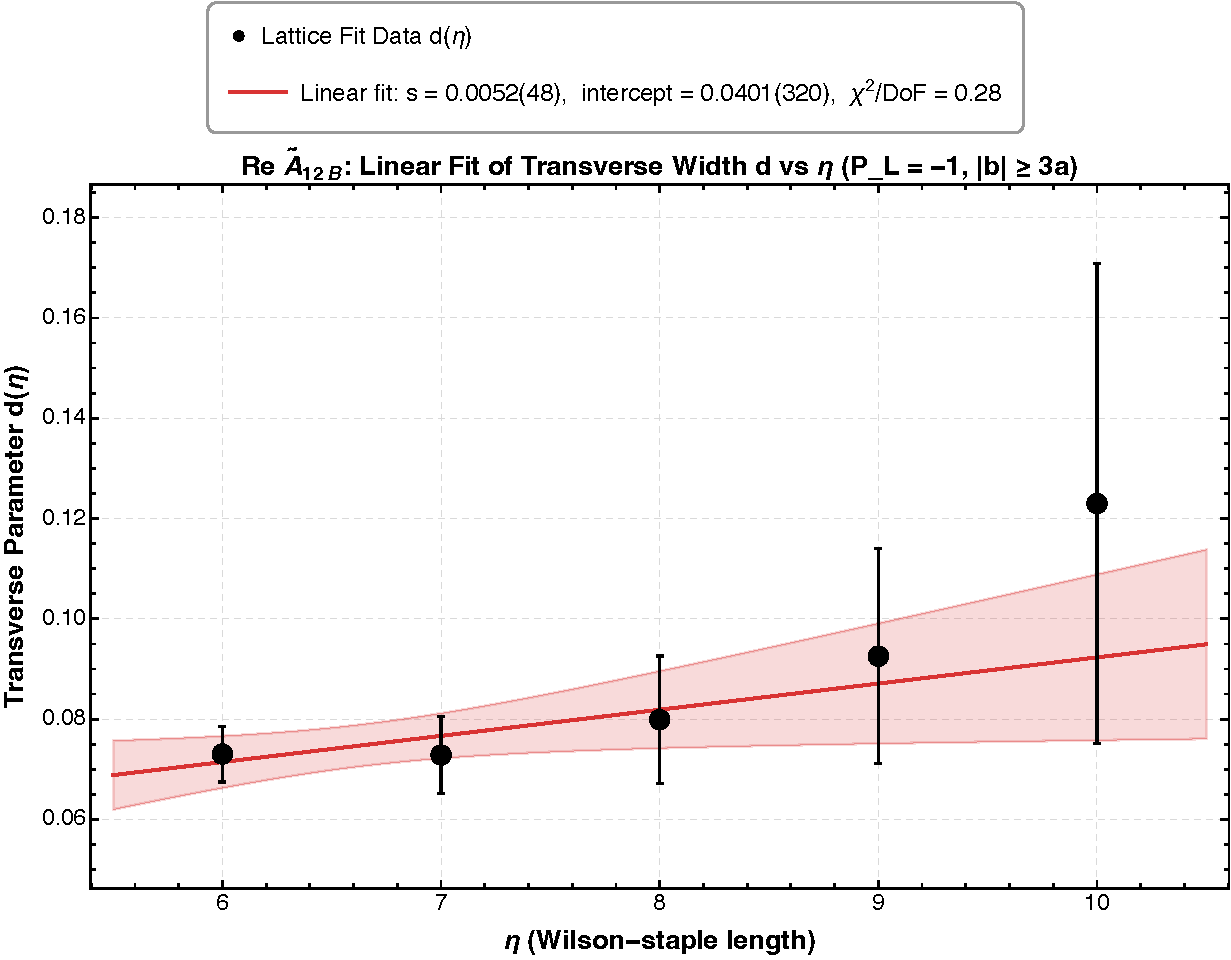
\includegraphics[width=\linewidth,height=.70\textheight,keepaspectratio]{fitting/ReA12B_d_eta_Independence_P1.pdf}
\par\small Slopes: $s_c=-0.0112(131)$, $s_d=0.0052(48)$; both compatible with zero.

\figsrc{Thesis: PowerLaw\_etaAsymptotic; ReA12B\_d\_eta\_Independence\_P1}
\end{frame}

\begin{frame}{Staple dependence of $c$: $\tAmp_{2B}^{\mathrm{Im}}$}
\centering
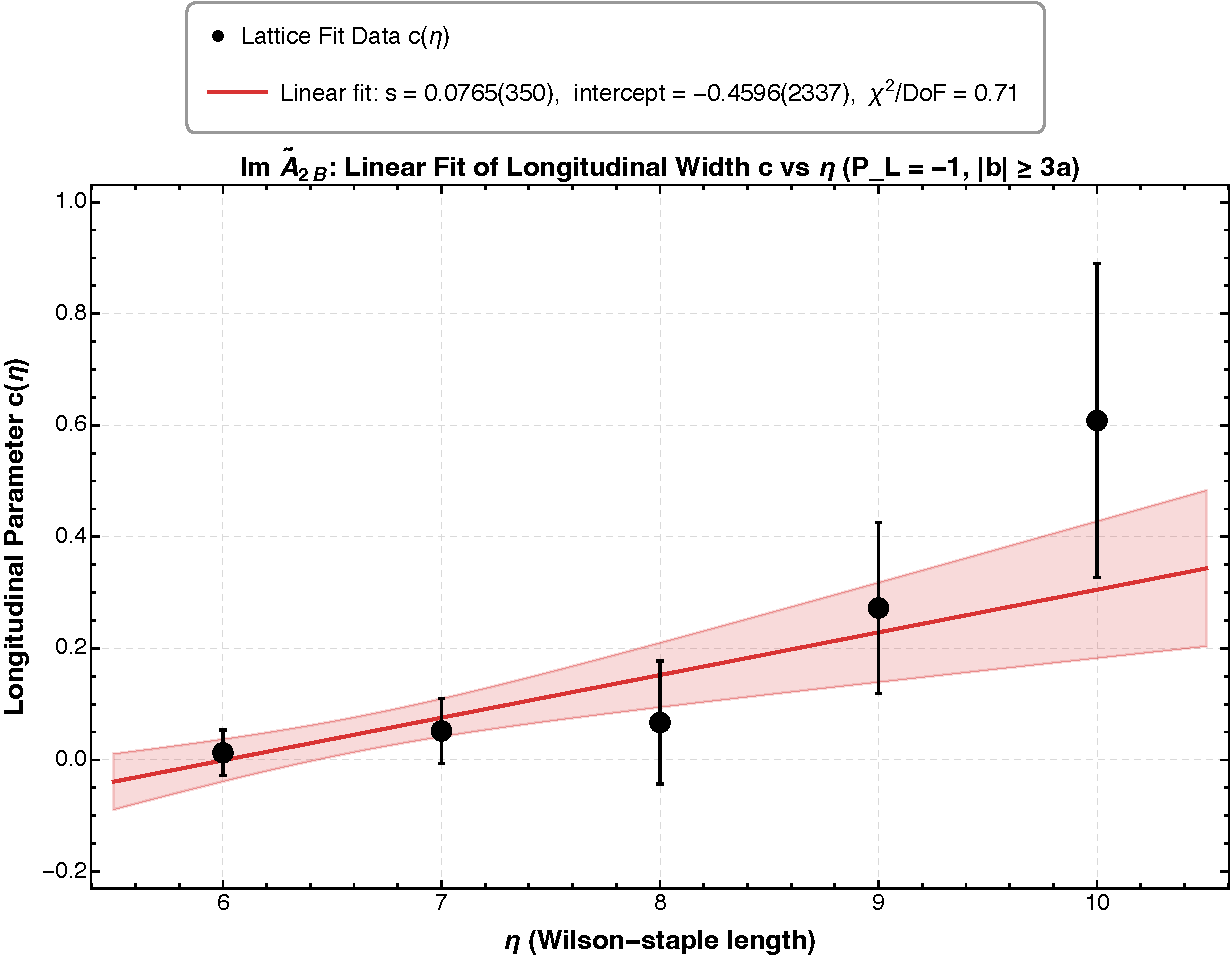
\includegraphics[width=\linewidth,height=.70\textheight,keepaspectratio]{fitting/ImA2B_c_eta_Independence_P1.pdf}
\par\small Slopes: $s_c=0.0765(350)$, $s_d=-0.0316(219)$; $c$ is about $2.2\sigma$ from zero. Constant widths are a modeling choice under these uncertainties.

\figsrc{Thesis: PowerLaw\_etaAsymptotic; ImA2B\_c\_eta\_Independence\_P1}
\end{frame}

\begin{frame}{Staple dependence of $d$: $\tAmp_{2B}^{\mathrm{Im}}$}
\centering
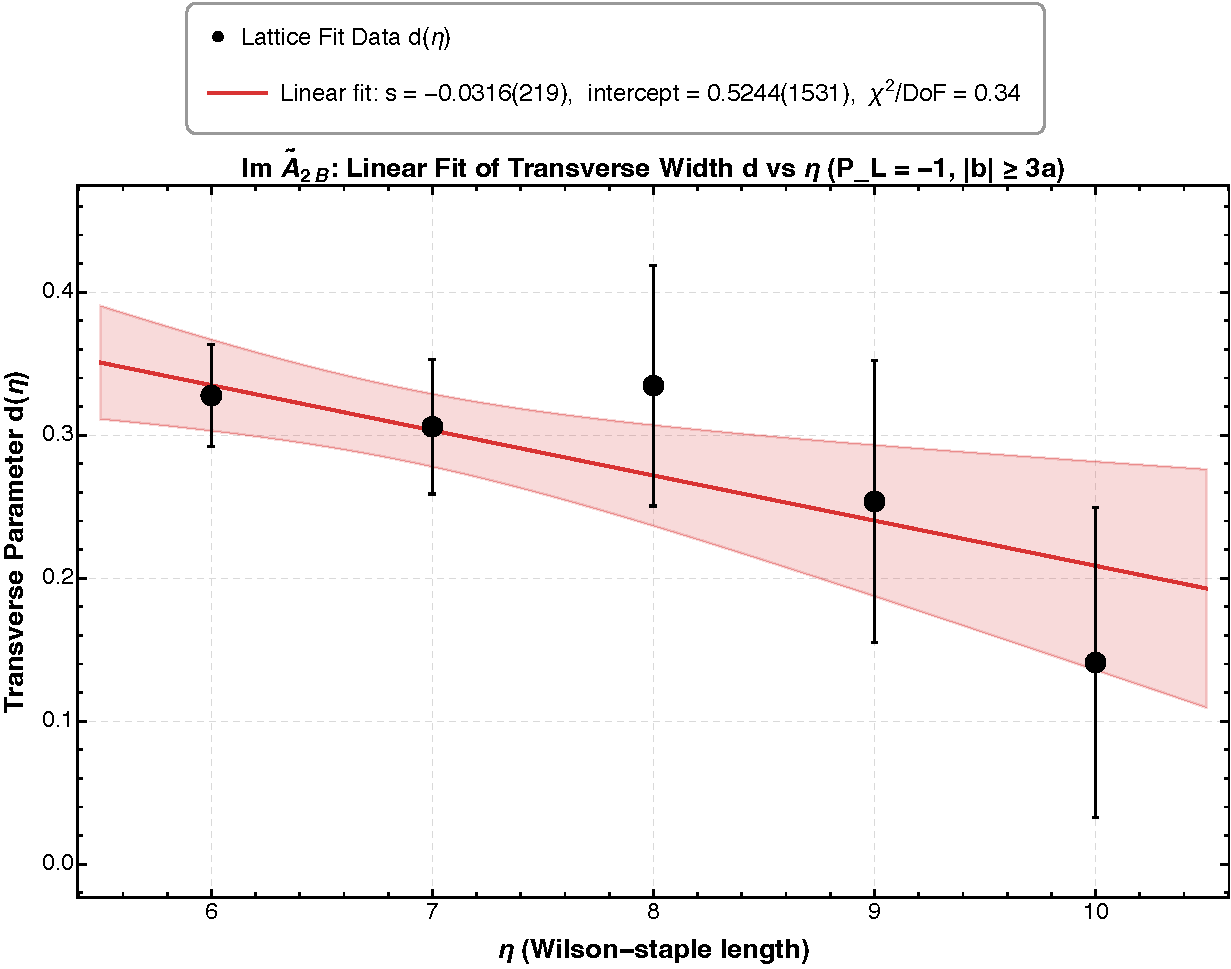
\includegraphics[width=\linewidth,height=.70\textheight,keepaspectratio]{fitting/ImA2B_d_eta_Independence_P1.pdf}
\par\small Slopes: $s_c=0.0765(350)$, $s_d=-0.0316(219)$; $c$ is about $2.2\sigma$ from zero. Constant widths are a modeling choice under these uncertainties.

\figsrc{Thesis: PowerLaw\_etaAsymptotic; ImA2B\_d\_eta\_Independence\_P1}
\end{frame}

\begin{frame}{Candidate selection combines several diagnostics}

\begin{itemize}
\item Fit quality, parameter stability, and AIC distinguish candidates with similar fixed-$\eta$ curves.
\item The thesis favors $c_2(\eta)=c(1-k_1/\eta-k_2/\eta^2)$ after examining the Fourier profile jointly with the imaginary amplitude.
\item For positive $x$, $\bar q(x)=-f_1(-x)$. The thesis uses suppression at $x\lesssim-0.2$ as a model-selection criterion for the negative-$x$ contribution.
\item Compare the integrated shift with previous $\nu=0$ lattice calculations; both real amplitudes and the imaginary unpolarized contribution enter the finite-$x$ integrals.
\end{itemize}
\[\langle k_y\rangle_{TU}^{[1]}=m_N\frac{\int dx\,\tilde f_{1T}^{\perp(1)}}{\int dx\,\tilde f_1^{(0)}}.\]
\figsrc{Thesis: Fitting Methodologies and Stability Analysis}
\end{frame}

\begin{frame}{The selected three-amplitude model}

\begin{align*}
\tAmp_{2B}^{\mathrm{Re}}&=\frac{a e^{-f\eta}}{[1+(d+c(1-k_1/\eta-k_2/\eta^2))b_L^2+db_T^2]^j},\\[3mm]
\tAmp_{12B}^{\mathrm{Re}}&=\frac{-a'e^{-f\eta}}{[1+(c'+d')b_L^2+d'b_T^2]^{j'}},\\[3mm]
\tAmp_{2B}^{\mathrm{Im}}&=\frac{a''b_L e^{-f\eta}}{[1+(c''+d'')b_L^2+d''b_T^2]^{j''}}.
\end{align*}
Shared $f$; independent spatial shape parameters for each amplitude.\par
$\tAmp_{12B}^{\mathrm{Im}}$ is omitted because the measured signal is consistent with zero.
\figsrc{Thesis: Fitting Methodologies and Stability Analysis}
\end{frame}

\begin{frame}{Full covariance in the simultaneous fit}

\[\bar y_i=\frac1{N_J}\sum_{k=1}^{N_J}y_i^{(k)},\qquad
C_{ij}=\frac{N_J-1}{N_J}\sum_{k=1}^{N_J}(y_i^{(k)}-\bar y_i)(y_j^{(k)}-\bar y_j).\]
\[\chi^2_{\rm data}(\mathbf p)=\sum_{i,j}[\bar y_i-F_i(\mathbf p)]C^{-1}_{ij}[\bar y_j-F_j(\mathbf p)].\]
\begin{itemize}
\item The combined data vector includes all retained coordinates and all three amplitudes at one momentum.
\item Cross-correlations matter because amplitudes use the same gauge configurations. Ignoring them changes the weighting and can misestimate uncertainties.
\item The implementation uses Gaussian priors and minimizes $\chi^2_{\rm aug}$, not just $\chi^2_{\rm data}$. Jackknife refits propagate the resulting parameter fluctuations.
\end{itemize}
\figsrc{Thesis: Fitting Methodologies and Stability Analysis}
\end{frame}

\begin{frame}{Actual simultaneous-fit objective and priors}
\[\chi^2_{\rm aug}=\chi^2_{\rm data}+\sum_{r=1}^{15}\left(\frac{p_r-\mu_r}{\sigma_r}\right)^2,
\qquad\sigma_r=0.05\quad\text{for all 15 parameters}.\]
\small\renewcommand{\arraystretch}{1.4}
\begin{tabular}{ll|ll|ll}\toprule
Real unpolarized & $\mu$ & Imaginary unpolarized & $\mu$ & Real Sivers / shared & $\mu$\\\midrule
$a$ & $4.01$ & $a''$ & $0.26$ & $a'$ & $0.6$\\
$c$ & $0.146$ & $c''$ & $0.3$ & $c'$ & $0.02$\\
$d$ & $0.094$ & $d''$ & $0.2$ & $d'$ & $0.02$\\
$k_1$ & $12.27$ & $j''$ & $1$ & $j'$ & $2$\\
$k_2$ & $-36.2$ & & & $f$ & $0.5$\\
$j$ & $2.06$ & & & & \\\bottomrule
\end{tabular}
\par\medskip All parameters are prior-constrained. The reported \texttt{lsqfit} statistic is $\chi^2_{\rm aug}/N_{\rm data}$; its degrees of freedom count includes the prior observations. It is not directly the same statistic as the earlier unregularized candidate fits.
\figsrc{Source: save\_h5\_A12B\_A2B/SimultaniousFit/SimultaneousFit\_A12bA2B.py, lines 197--247}
\end{frame}
\begin{frame}{Fourier continuation and integrability conditions}

\[D_R=[1+c(1-k_1/\eta-k_2/\eta^2)\nu^2/P_L^2+db^2]^j,\]
\[D_S=[1+c'\nu^2/P_L^2+d'b^2]^{j'},\qquad
D_I=[1+c''\nu^2/P_L^2+d''b^2]^{j''}.\]
\begin{itemize}
\item Cancel the common $e^{-f\eta}$ in the ratio; then take $\eta\to\infty$, so $c(\eta)\to c$.
\item For $A+B\nu^2$ with $A>0$, $B>0$, the even profile is absolutely integrable for $j>1/2$.
\item The odd profile $\nu(A+B\nu^2)^{-j''}$ needs $j''>1$ for absolute integrability. The highest-momentum fit lies close to this boundary.
\item Positivity must be checked in the continuation used for the transform; a positive spatial-grid denominator alone is insufficient.
\end{itemize}
\figsrc{Thesis: Fitting Methodologies and Stability Analysis}
\end{frame}

\begin{frame}{Real cosine and sine transforms: signs made explicit}

\begin{align*}
E(x,b^2)&=\int_{-\infty}^{\infty}\frac{d\nu}{2\pi}\cos(x\nu)R(\nu,b^2),\\
O(x,b^2)&=\int_{-\infty}^{\infty}\frac{d\nu}{2\pi}\sin(x\nu)I(\nu,b^2),\\
S(x,b^2)&=\int_{-\infty}^{\infty}\frac{d\nu}{2\pi}\cos(x\nu)S_0(\nu,b^2).
\end{align*}
$R,I,S_0$ denote the three selected amplitudes after removal of their common factor and the $\eta\to\infty$ limit.\par
\[\tilde f_1^{(0)}=2(E-O),\quad\tilde f_{1T}^{\perp(1)}=-2S,\quad
\langle k_y\rangle_{TU}=-m_N\frac{S}{E-O}.\]
The sine contribution $O$ is real; $i\int e^{ix\nu}I\,d\nu/(2\pi)=-O$.
\figsrc{Thesis: Fitting Methodologies and Stability Analysis}
\end{frame}

\begin{frame}{Integrated cross-checks and normalization}

\[\int_{-\infty}^{\infty}dx\,E(x,b^2)=R(0,b^2),\qquad
\int_{-\infty}^{\infty}dx\,O(x,b^2)=0,\]
\[m_N\frac{\int_{-\infty}^{\infty}dx\,\tilde f_{1T}^{\perp(1)}}
{\int_{-\infty}^{\infty}dx\,\tilde f_1^{(0)}}=-m_N\frac{S_0(0,b^2)}{R(0,b^2)}.\]
\begin{itemize}
\item The $1/(2\pi)$ Fourier normalization gives these identities.
\item The thesis tables compare $(-\infty,\infty)$, $[-1,1]$, $[-1,0]$, and $[0,1]$ at $b^2=9a^2$.
\item The ratio of integrals is distinct from the integral of the $x$-dependent ratio.
\item A common soft factor cancels in the shift; plotted individual transforms follow the thesis normalization convention.
\end{itemize}
\figsrc{Thesis: Fitting Methodologies and Stability Analysis}
\end{frame}

\begin{frame}{Simultaneous fit parameters: $P_L=-1$}
\small $|\vect b|\ge3a$, $6\le\eta\le10$; reported $\chi^2_{\rm aug}/N_{\rm data}=1.85(10)$.\par\medskip
\begin{columns}[t]\begin{column}{.32\textwidth}\centering $\tAmp_{2B}^{\mathrm{Re}}$\par\medskip\renewcommand{\arraystretch}{1.3}\begin{tabular}{cc}\toprule Parameter & Value\\\midrule
$a$ & $3.863(11)$ \\
$c$ & $0.336(40)$ \\
$d$ & $0.1630(74)$ \\
$k_1$ & $12.288(23)$ \\
$k_2$ & $-36.1965(45)$ \\
$j$ & $1.627(25)$ \\
$f$ & $0.4702(46)$ \\\bottomrule\end{tabular}\end{column}\begin{column}{.32\textwidth}\centering $\tAmp_{2B}^{\mathrm{Im}}$\par\medskip\renewcommand{\arraystretch}{1.3}\begin{tabular}{cc}\toprule Parameter & Value\\\midrule
$a''$ & $0.267(13)$ \\
$c''$ & $0.2253(69)$ \\
$d''$ & $0.2205(66)$ \\
$j''$ & $1.108(21)$ \\
$f$ & $0.4702(46)$ \\\bottomrule\end{tabular}\end{column}\begin{column}{.32\textwidth}\centering $\tAmp_{12B}^{\mathrm{Re}}$\par\medskip\renewcommand{\arraystretch}{1.3}\begin{tabular}{cc}\toprule Parameter & Value\\\midrule
$a'$ & $0.658(22)$ \\
$c'$ & $0.0773(46)$ \\
$d'$ & $0.0747(43)$ \\
$j'$ & $2.0054(90)$ \\
$f$ & $0.4702(46)$ \\\bottomrule\end{tabular}\end{column}\end{columns}
\figsrc{Thesis: SimultaneousFitsCov/Fit\_Table\_PL-1\_bmin3.tex}
\end{frame}

\begin{frame}{Global fit: $\tAmp_{2B}^{\mathrm{Re}}$, $P_L=-1$}
\centering
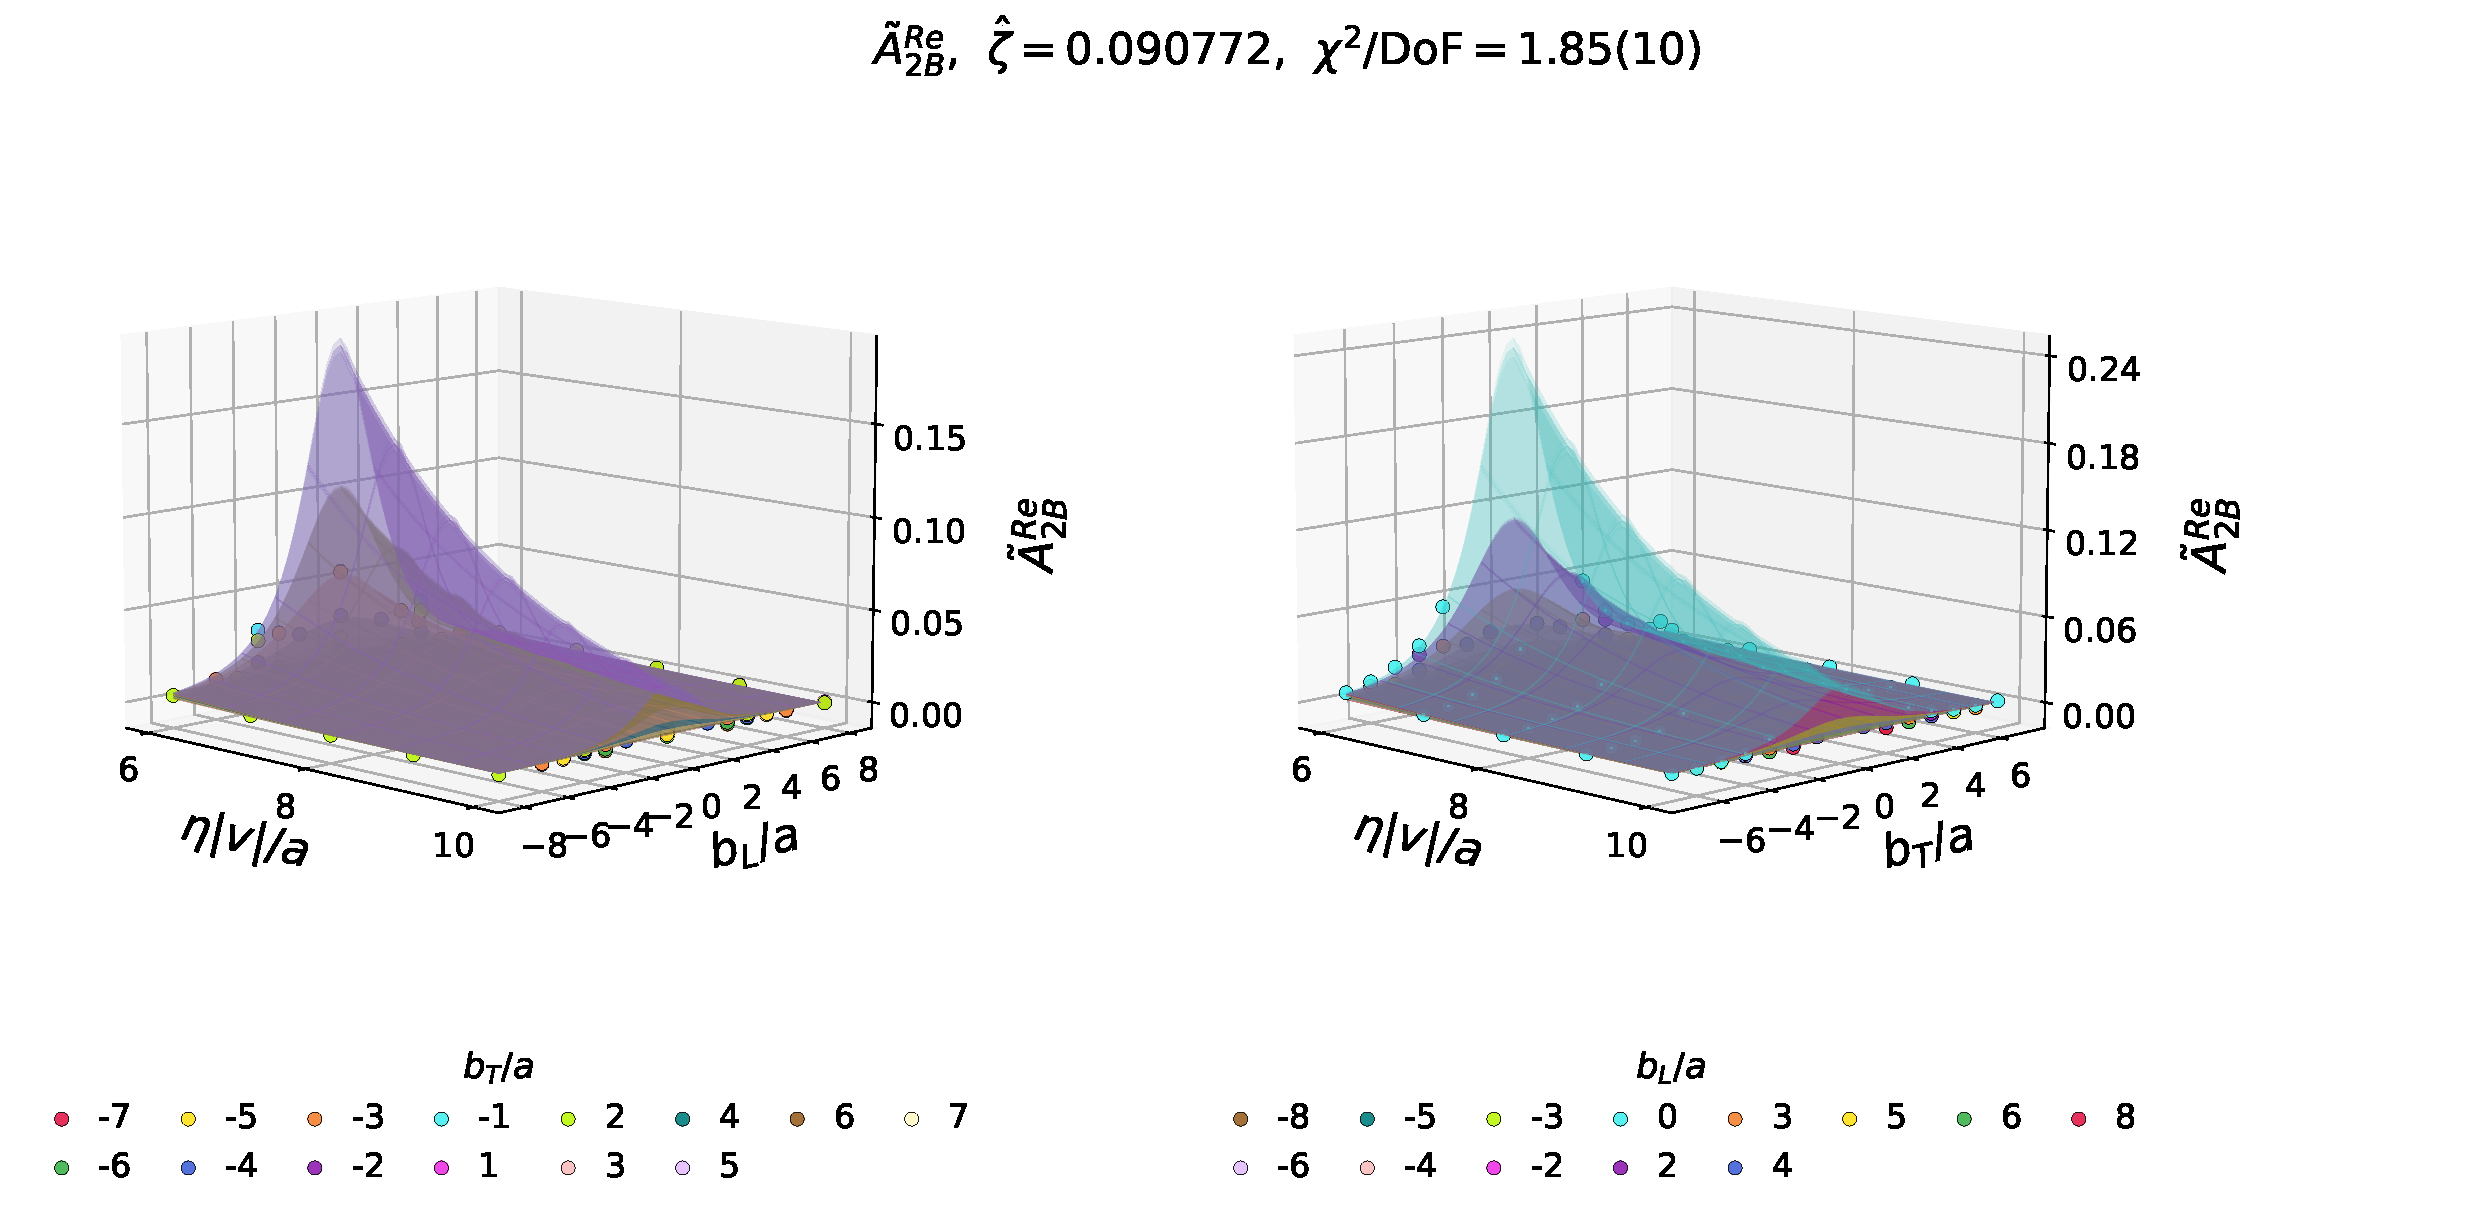
\includegraphics[width=\linewidth,height=.70\textheight,keepaspectratio]{fitting/ReA2B_PL-1_WithFit_3D.pdf}
\par\small Spatial coordinates: $(b_L,b_T,\eta)$. All panels and data overlays retained.

\figsrc{Thesis: plots; ReA2B\_PL-1\_WithFit\_3D}
\end{frame}

\begin{frame}{Global fit: $\tAmp_{2B}^{\mathrm{Re}}$, $P_L=-1$}
\centering
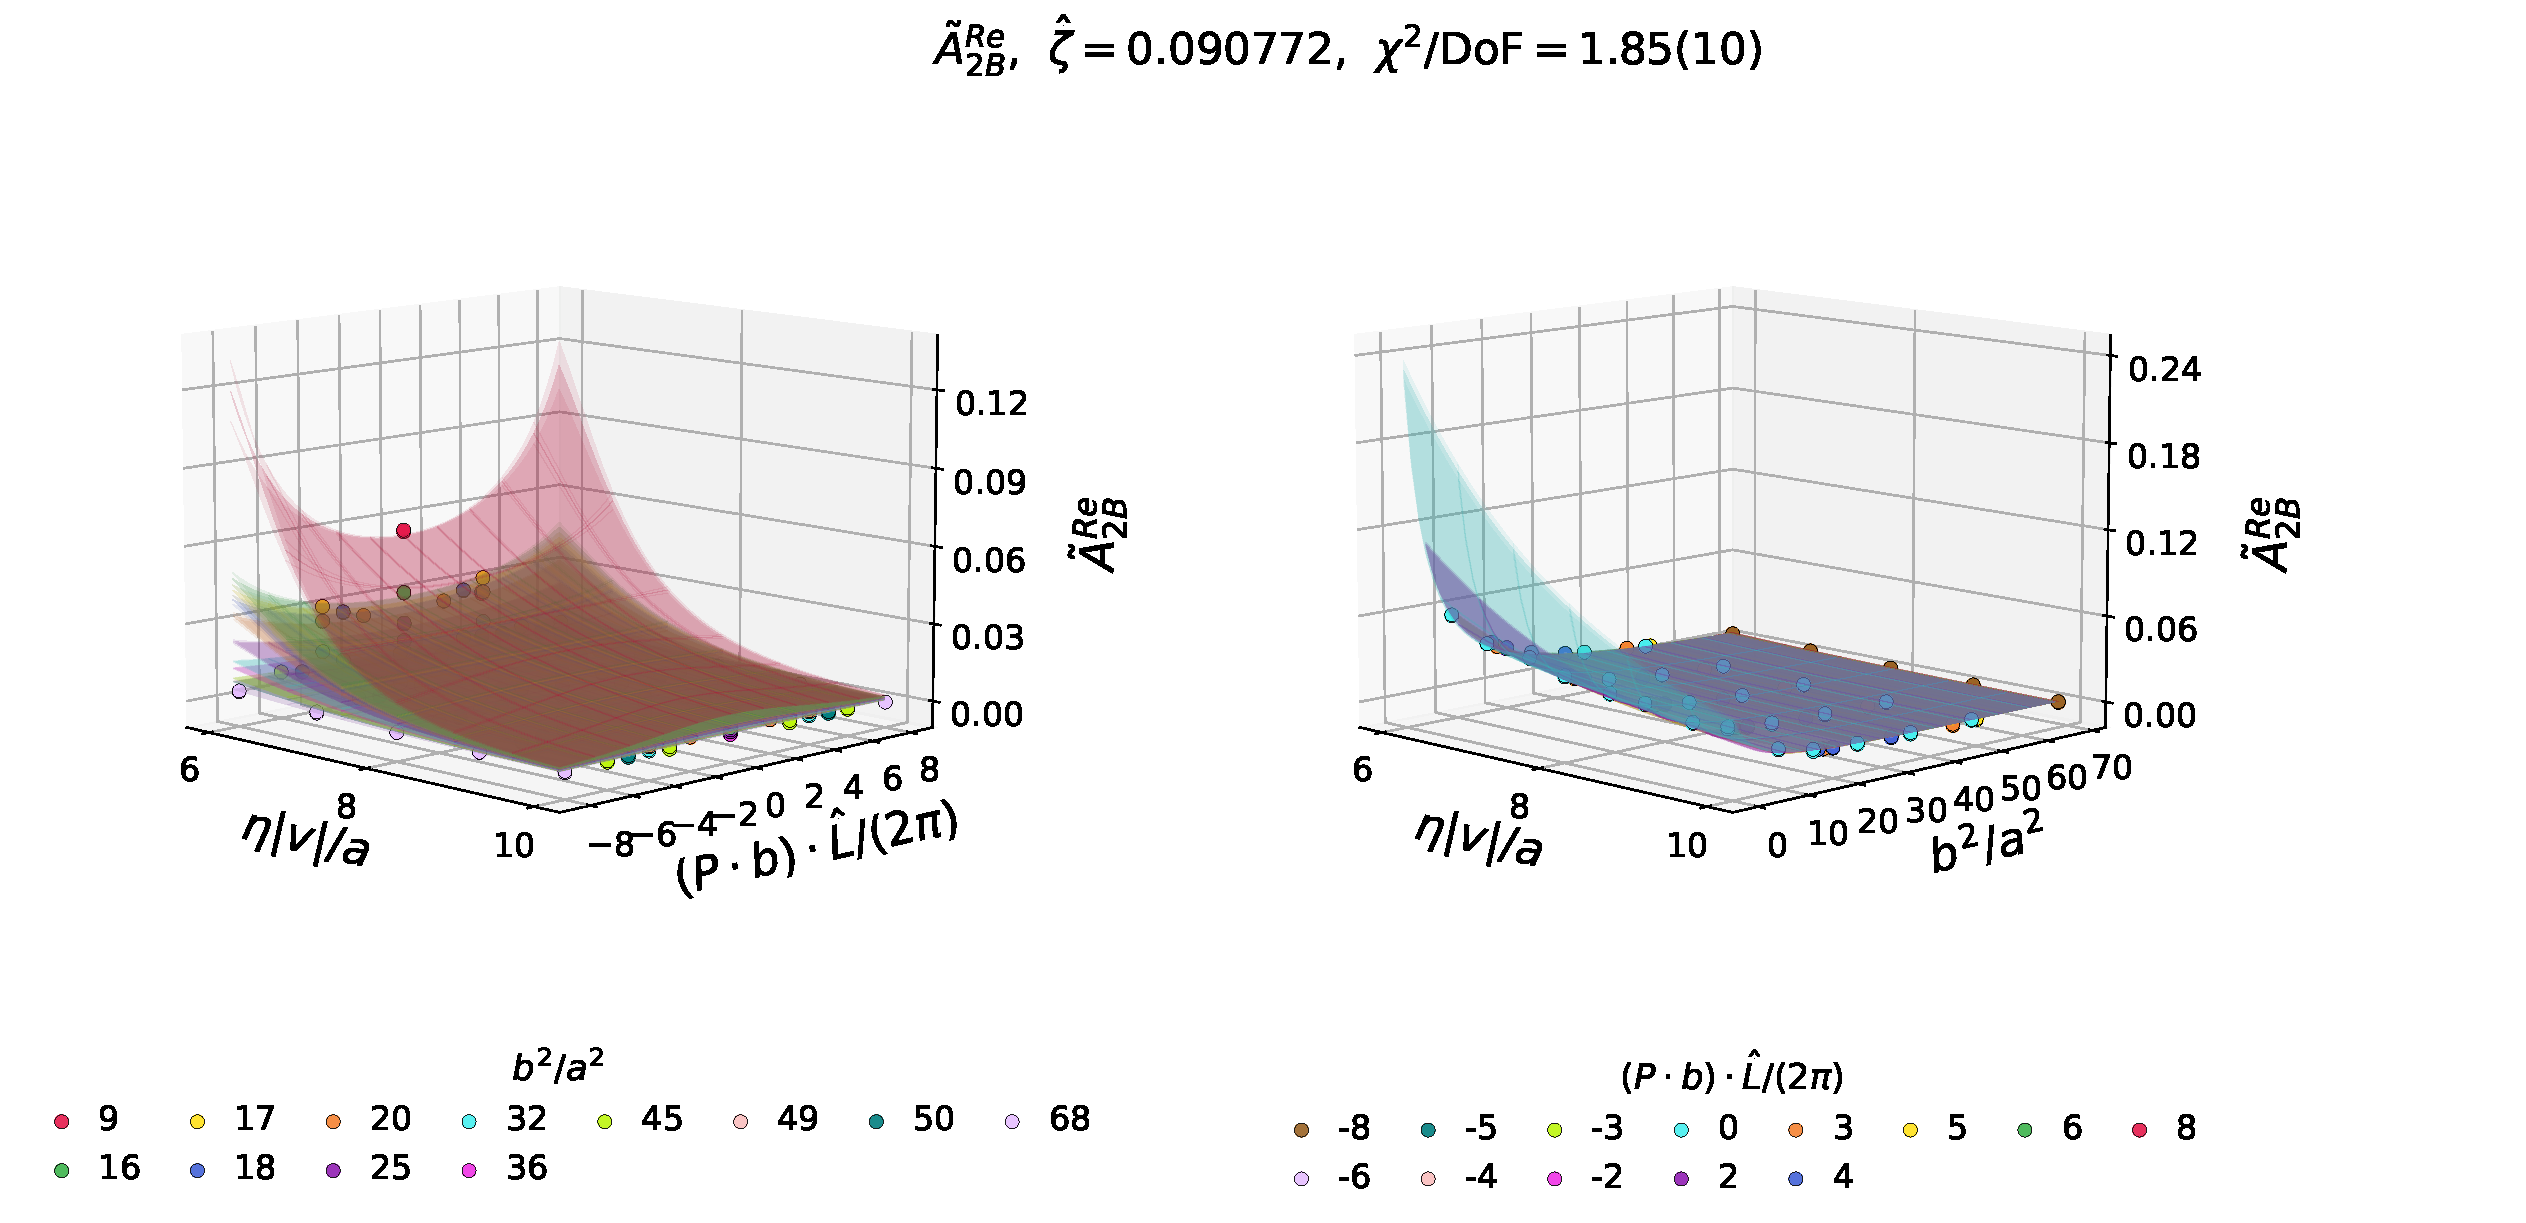
\includegraphics[width=\linewidth,height=.70\textheight,keepaspectratio]{fitting/ReA2B_Pb_bsq_PL-1_WithFit_3D.pdf}
\par\small Invariant coordinates: $(\nu,b^2,\eta)$. All panels and data overlays retained.

\figsrc{Thesis: plots; ReA2B\_Pb\_bsq\_PL-1\_WithFit\_3D}
\end{frame}

\begin{frame}{Fixed staple $\eta=8$: $\tAmp_{2B}^{\mathrm{Re}}$, $P_L=-1$}
\centering
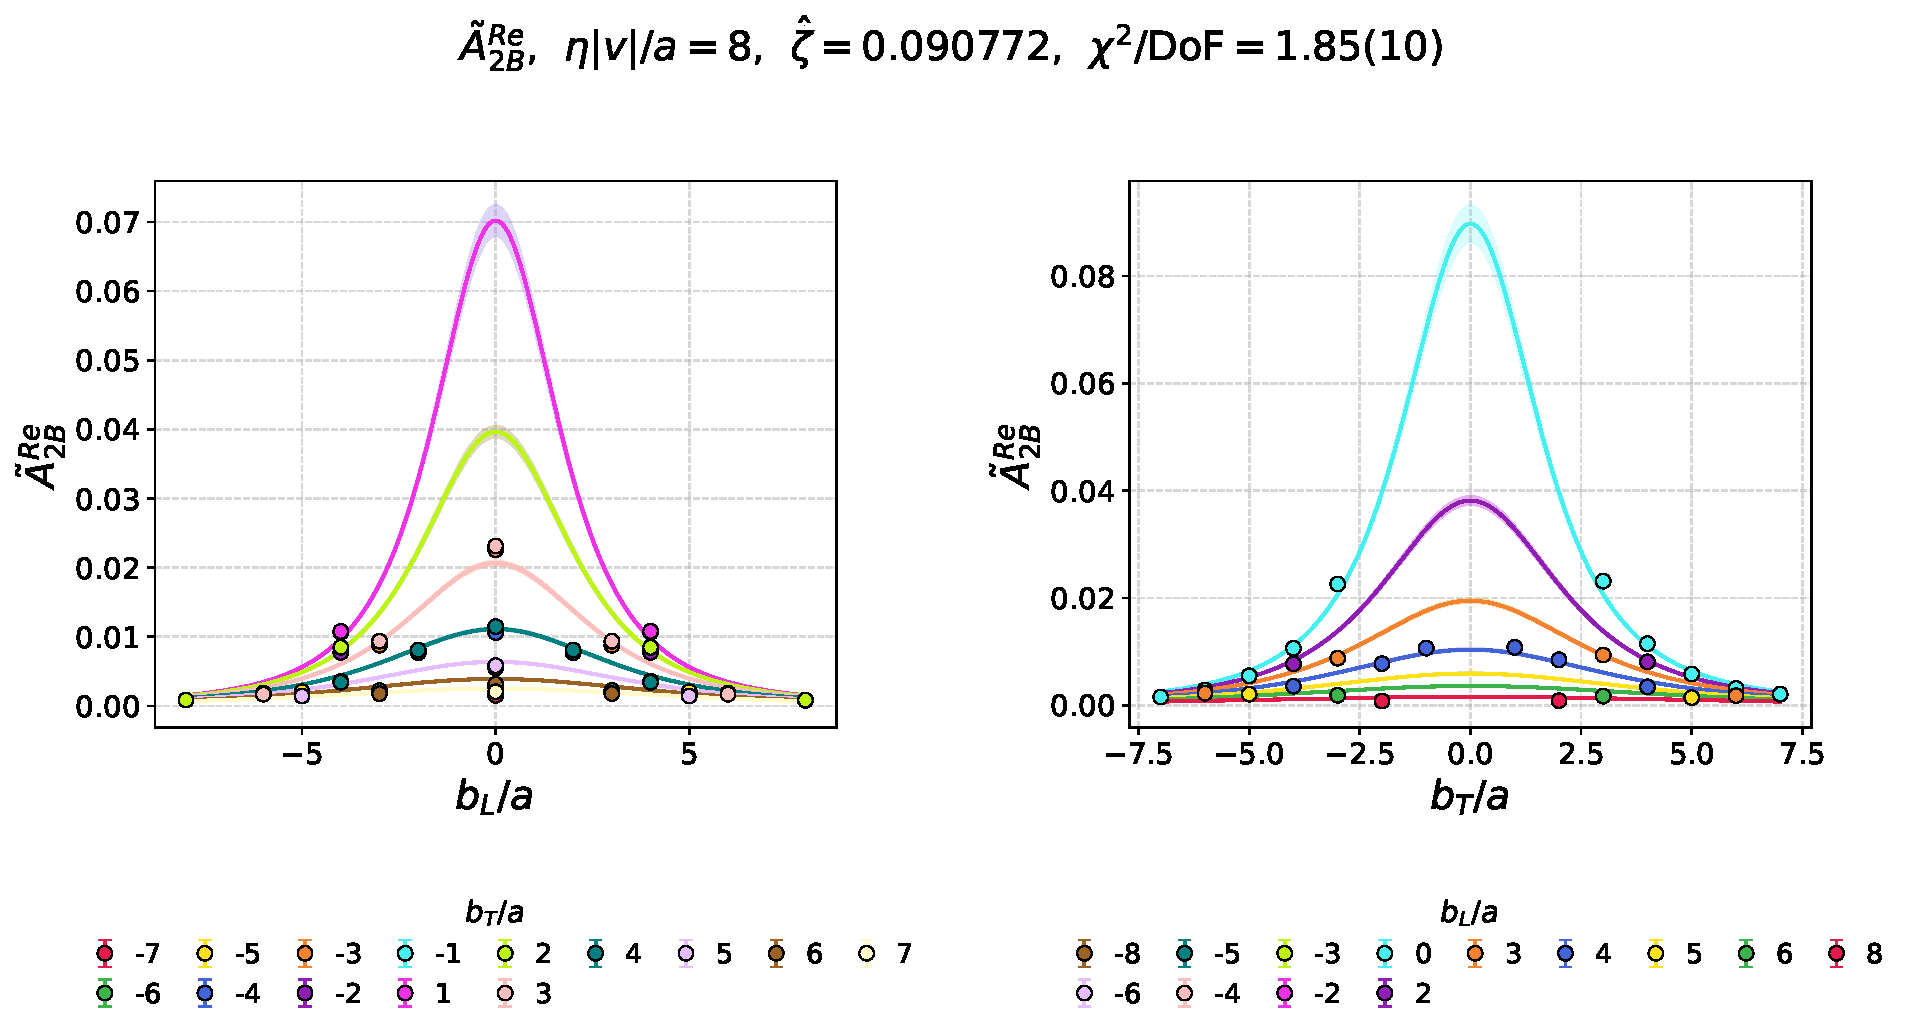
\includegraphics[width=\linewidth,height=.70\textheight,keepaspectratio]{fitting/ReA2B_eta8_PL-1_WithFit_2D.pdf}
\par\small Both spatial-coordinate slices. Same simultaneous fit, with Jackknife bands.

\figsrc{Thesis: plots; ReA2B\_eta8\_PL-1\_WithFit\_2D}
\end{frame}

\begin{frame}{Fixed staple $\eta=8$: $\tAmp_{2B}^{\mathrm{Re}}$, $P_L=-1$}
\centering
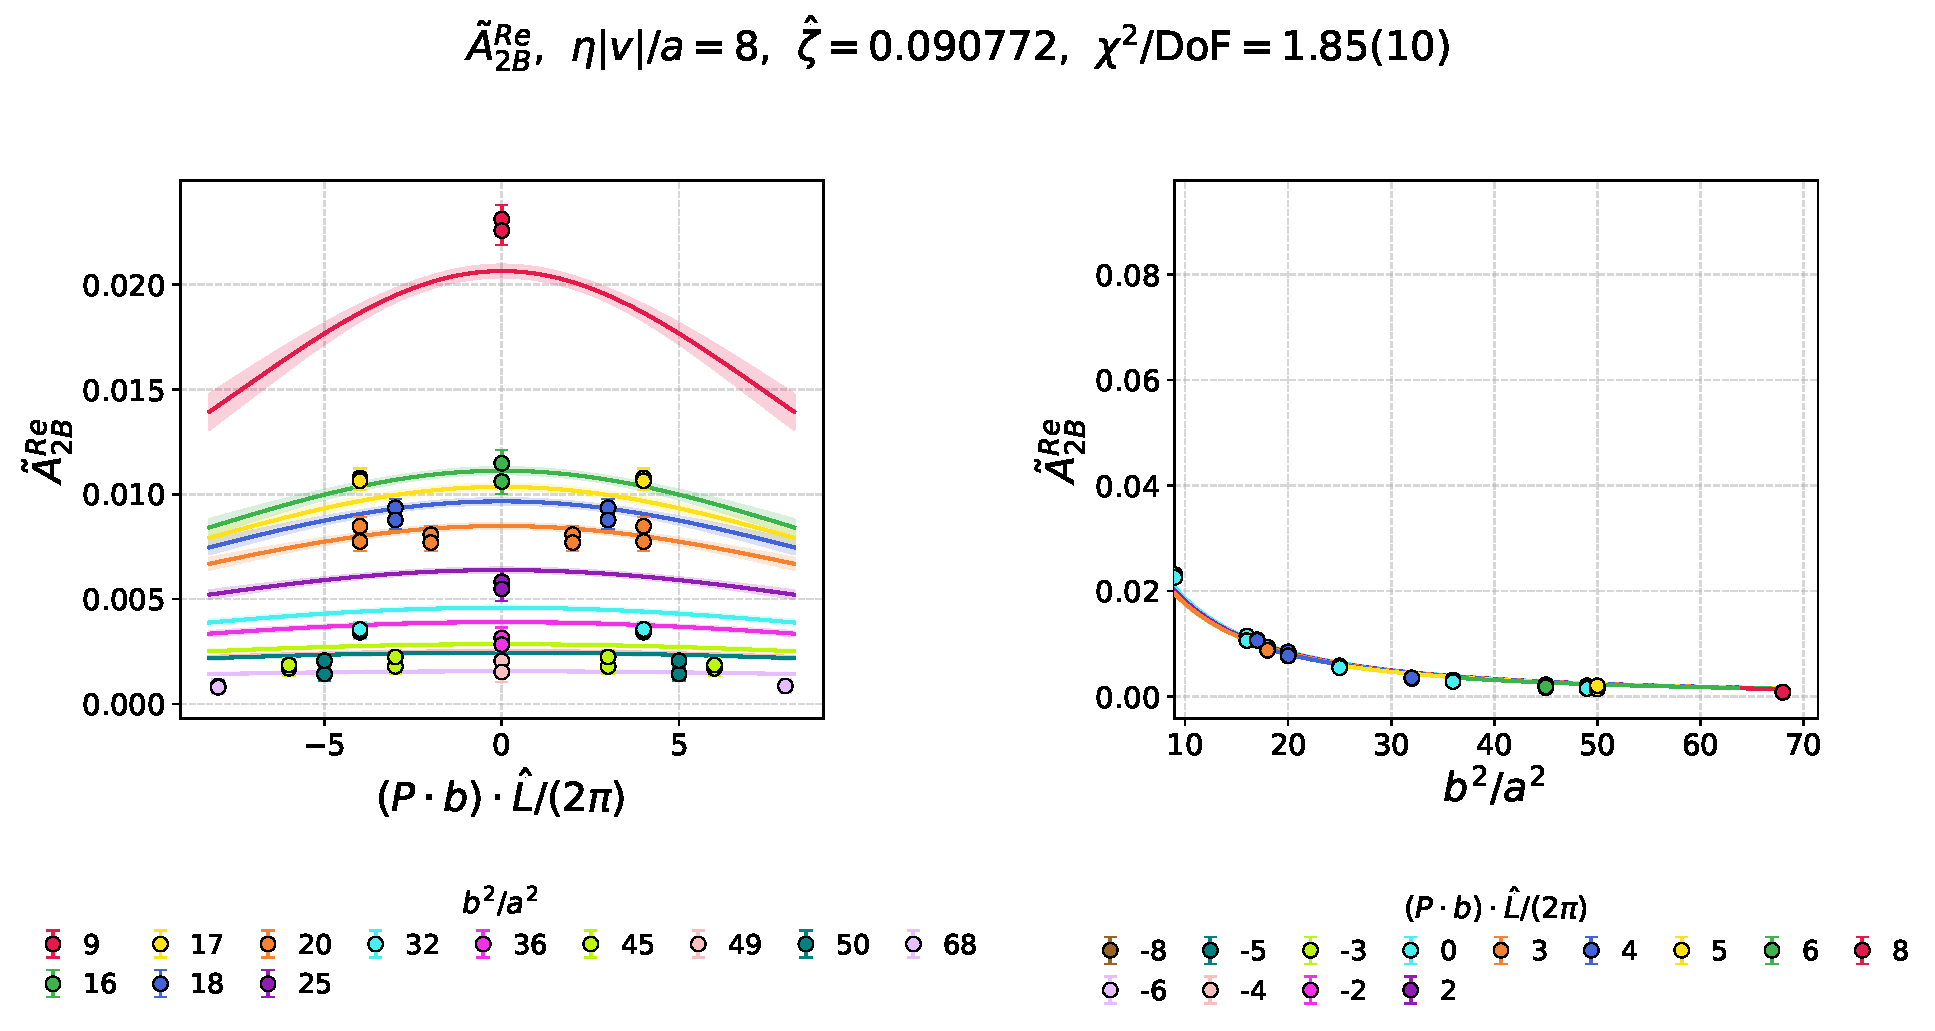
\includegraphics[width=\linewidth,height=.70\textheight,keepaspectratio]{fitting/ReA2B_Pb_bsq_eta8_PL-1_WithFit_2D.pdf}
\par\small Both invariant-coordinate slices. Same simultaneous fit, with Jackknife bands.

\figsrc{Thesis: plots; ReA2B\_Pb\_bsq\_eta8\_PL-1\_WithFit\_2D}
\end{frame}

\begin{frame}{Global fit: $\tAmp_{2B}^{\mathrm{Im}}$, $P_L=-1$}
\centering
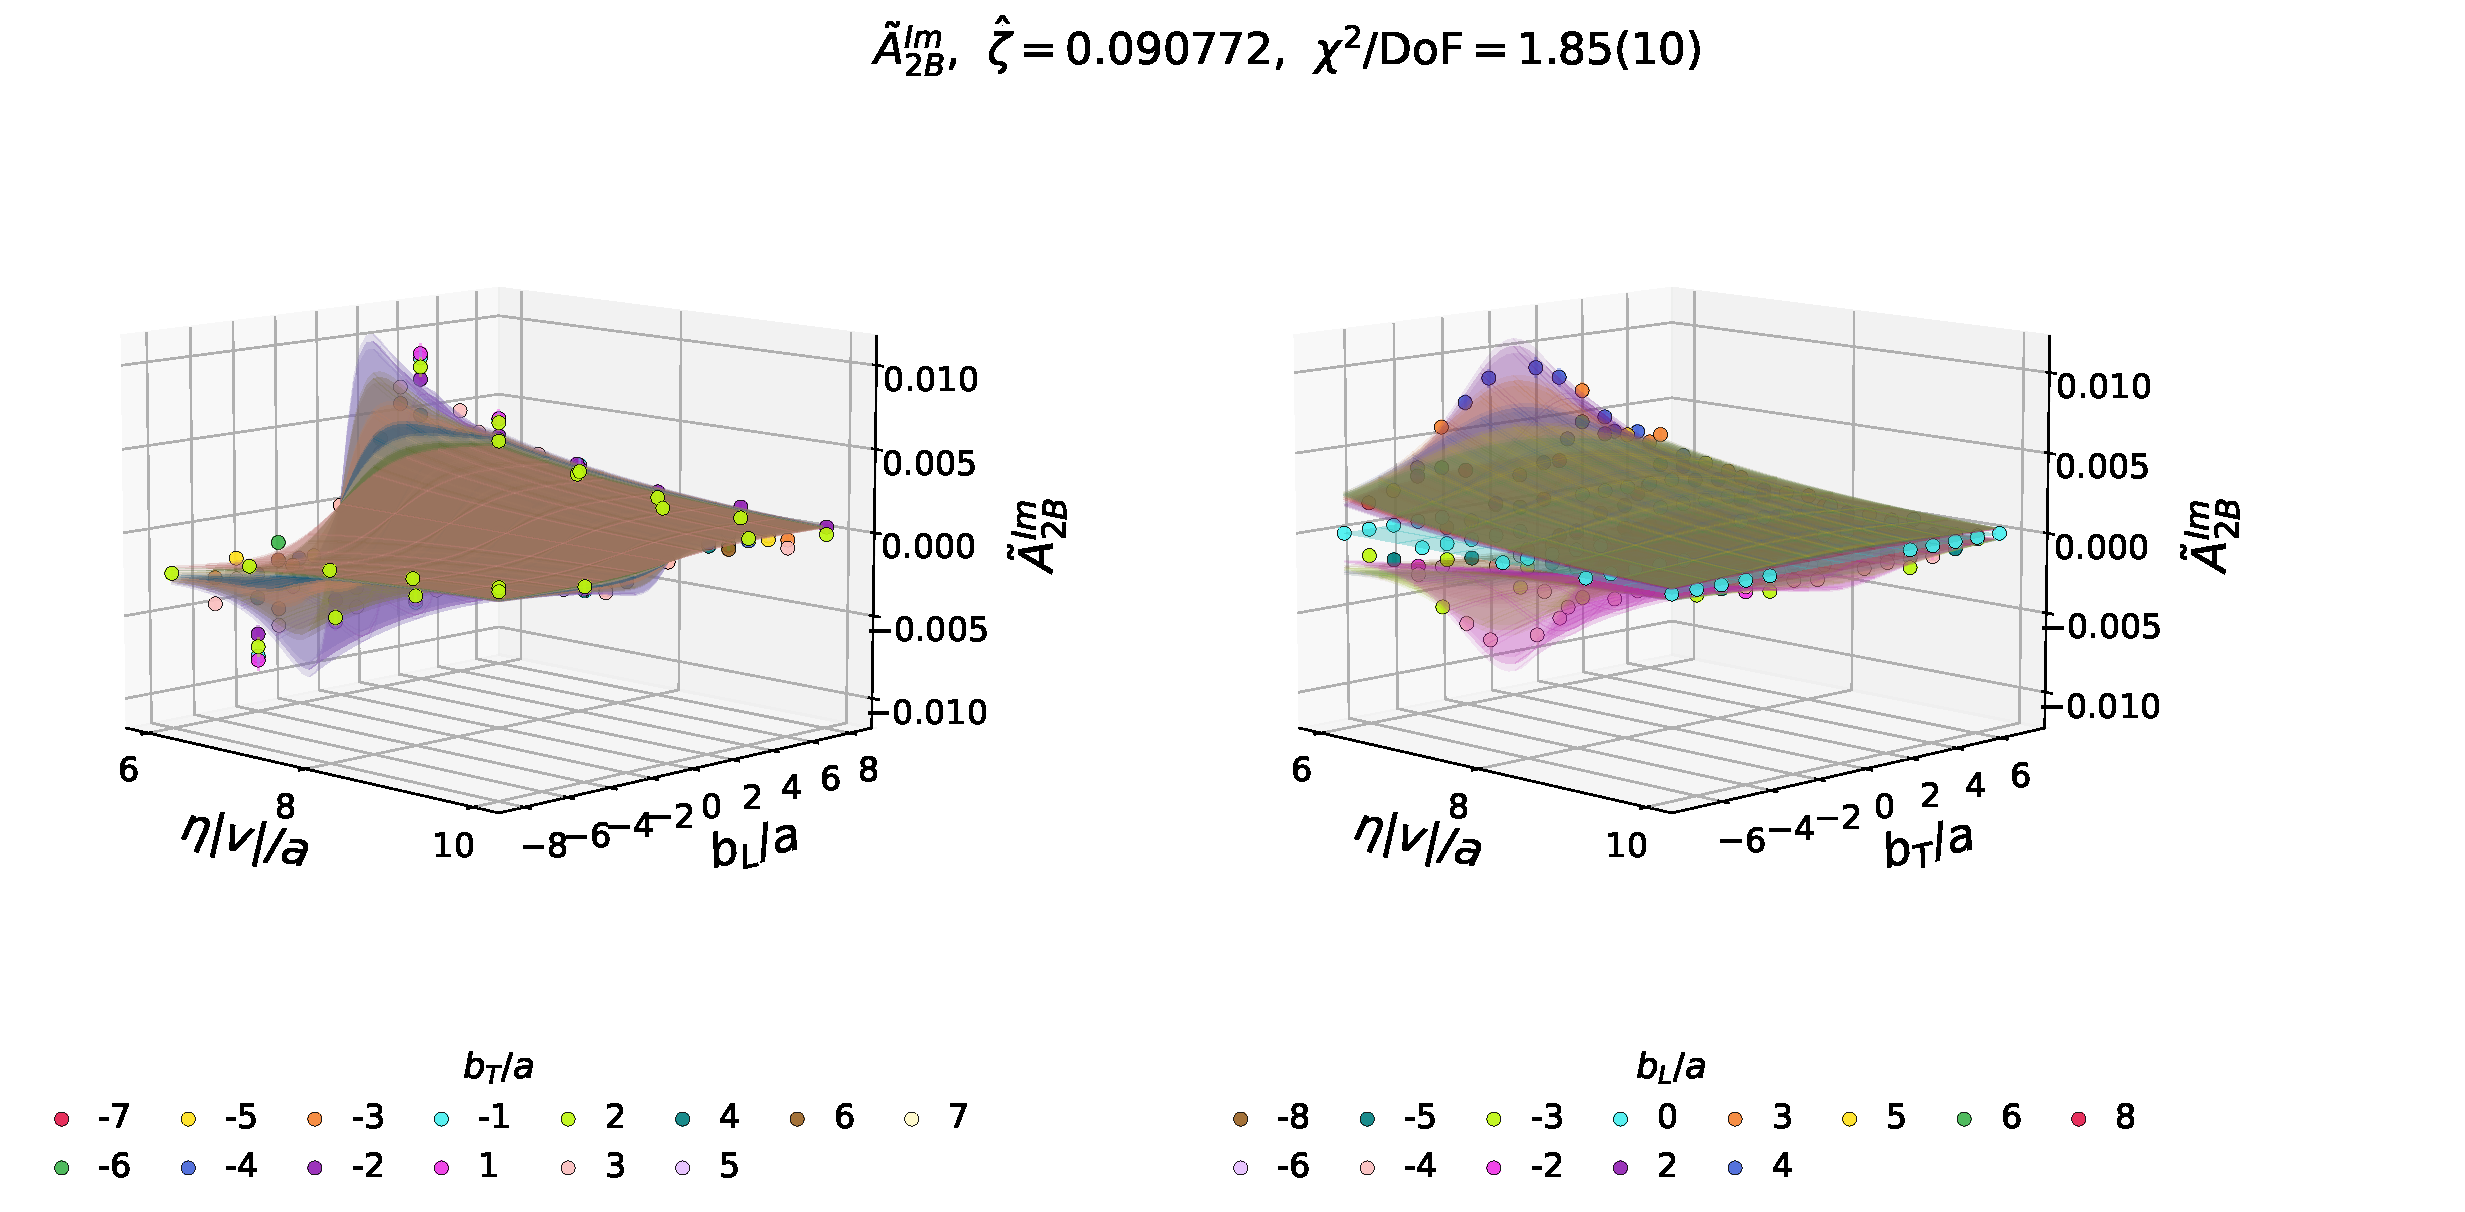
\includegraphics[width=\linewidth,height=.70\textheight,keepaspectratio]{fitting/ImA2B_PL-1_WithFit_3D.pdf}
\par\small Spatial coordinates: $(b_L,b_T,\eta)$. All panels and data overlays retained.

\figsrc{Thesis: plots; ImA2B\_PL-1\_WithFit\_3D}
\end{frame}

\begin{frame}{Global fit: $\tAmp_{2B}^{\mathrm{Im}}$, $P_L=-1$}
\centering
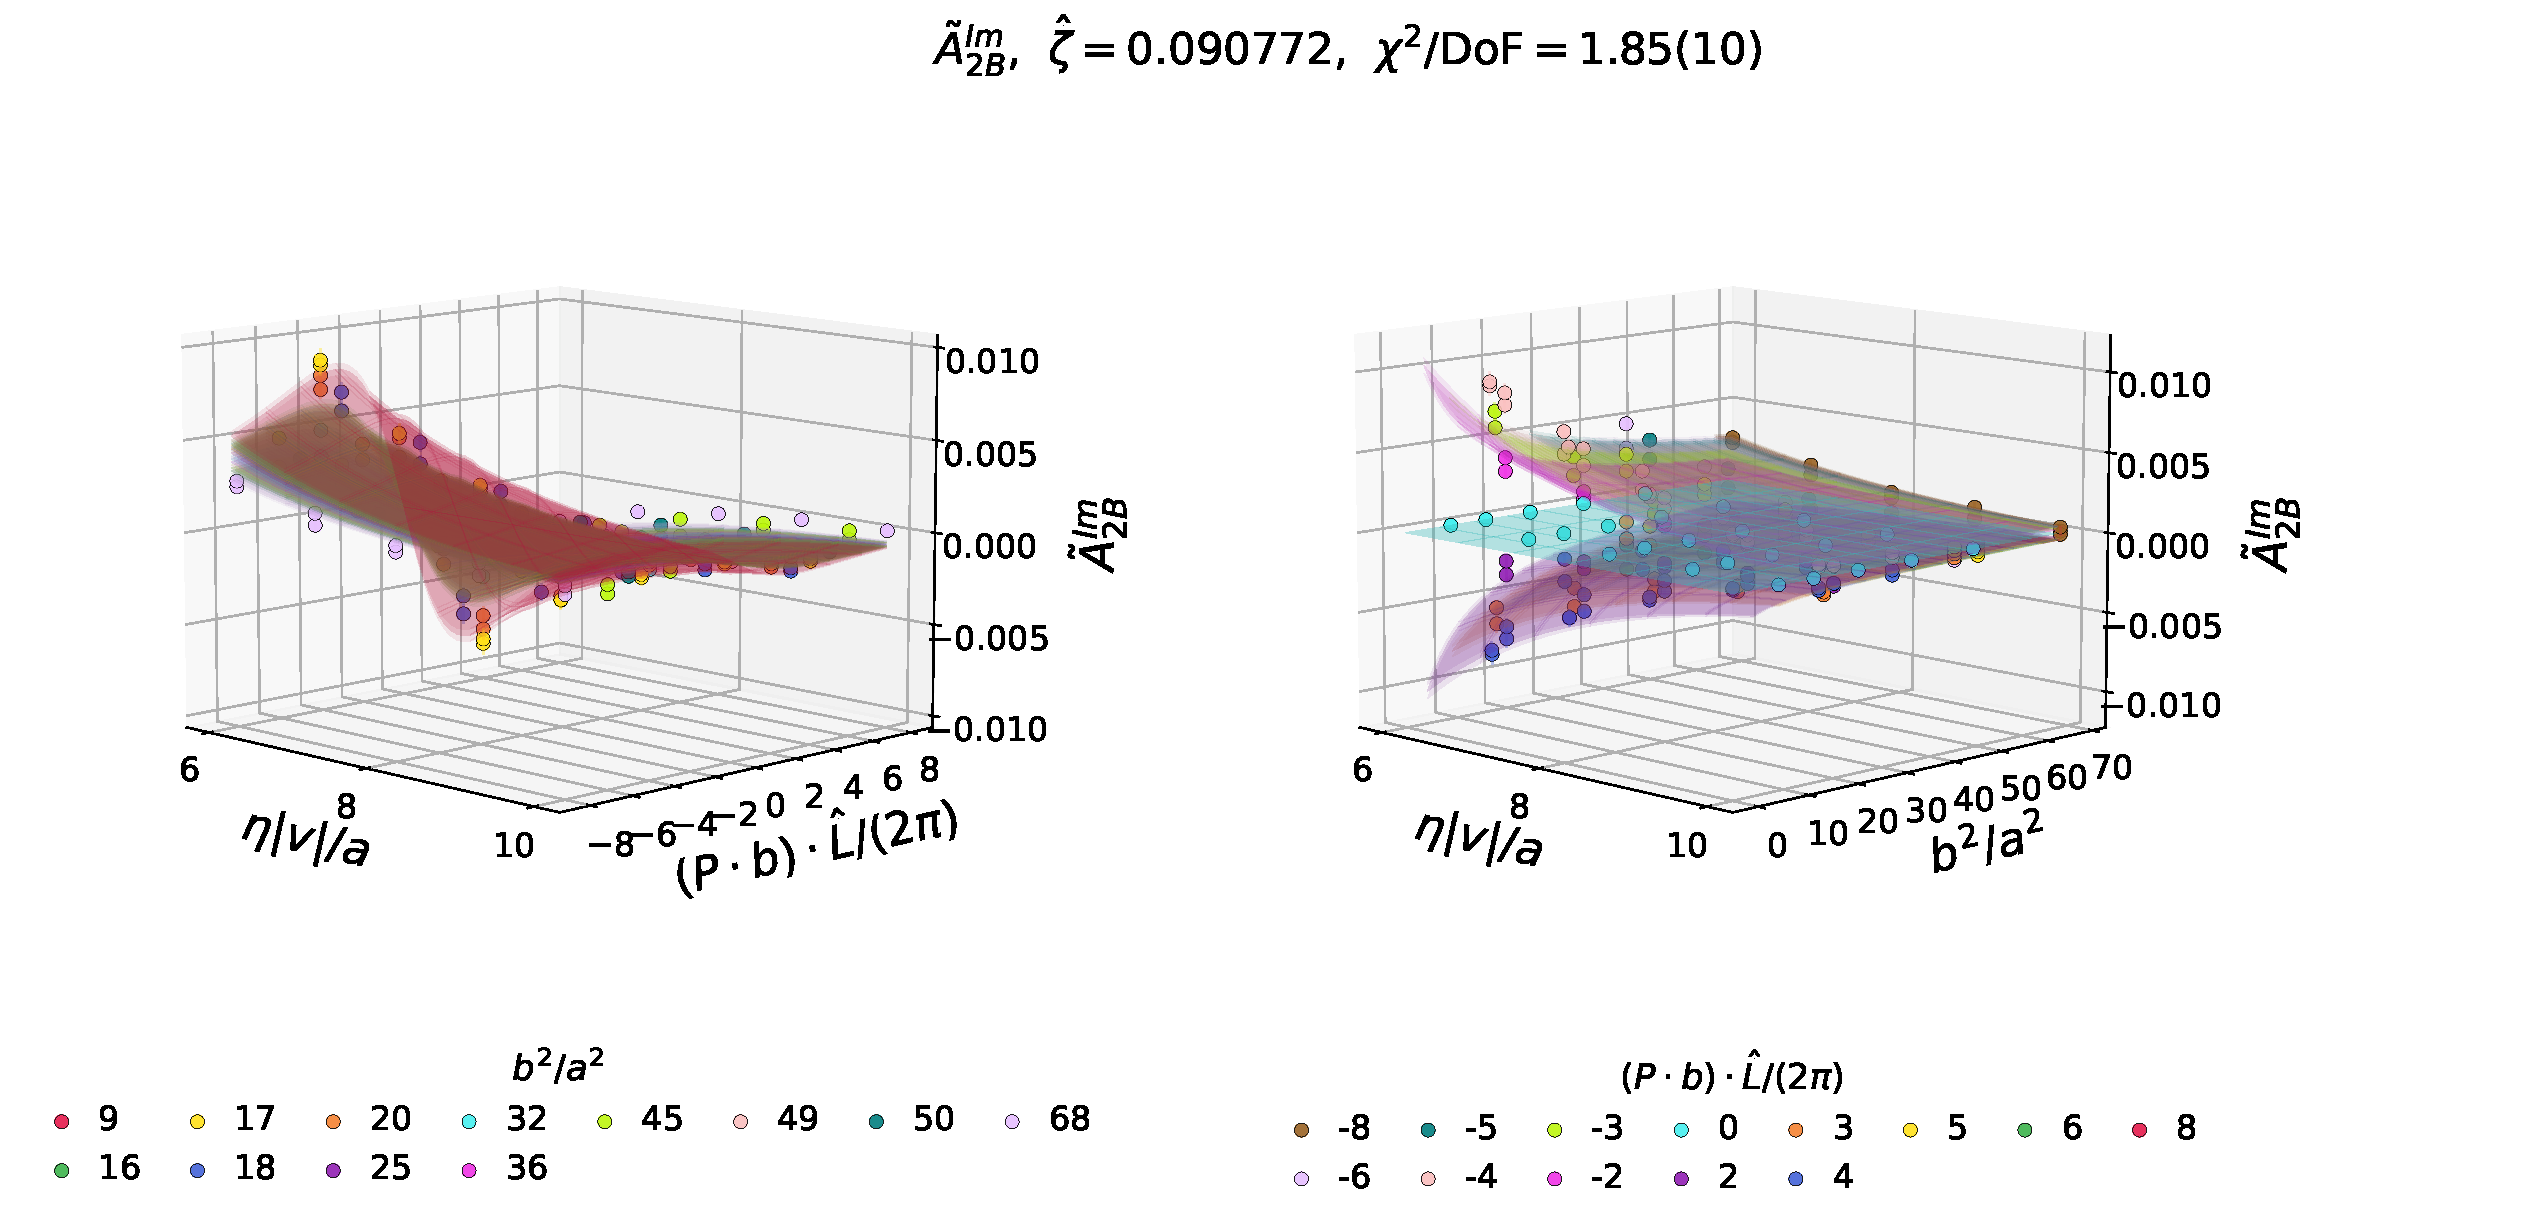
\includegraphics[width=\linewidth,height=.70\textheight,keepaspectratio]{fitting/ImA2B_Pb_bsq_PL-1_WithFit_3D.pdf}
\par\small Invariant coordinates: $(\nu,b^2,\eta)$. All panels and data overlays retained.

\figsrc{Thesis: plots; ImA2B\_Pb\_bsq\_PL-1\_WithFit\_3D}
\end{frame}

\begin{frame}{Fixed staple $\eta=8$: $\tAmp_{2B}^{\mathrm{Im}}$, $P_L=-1$}
\centering
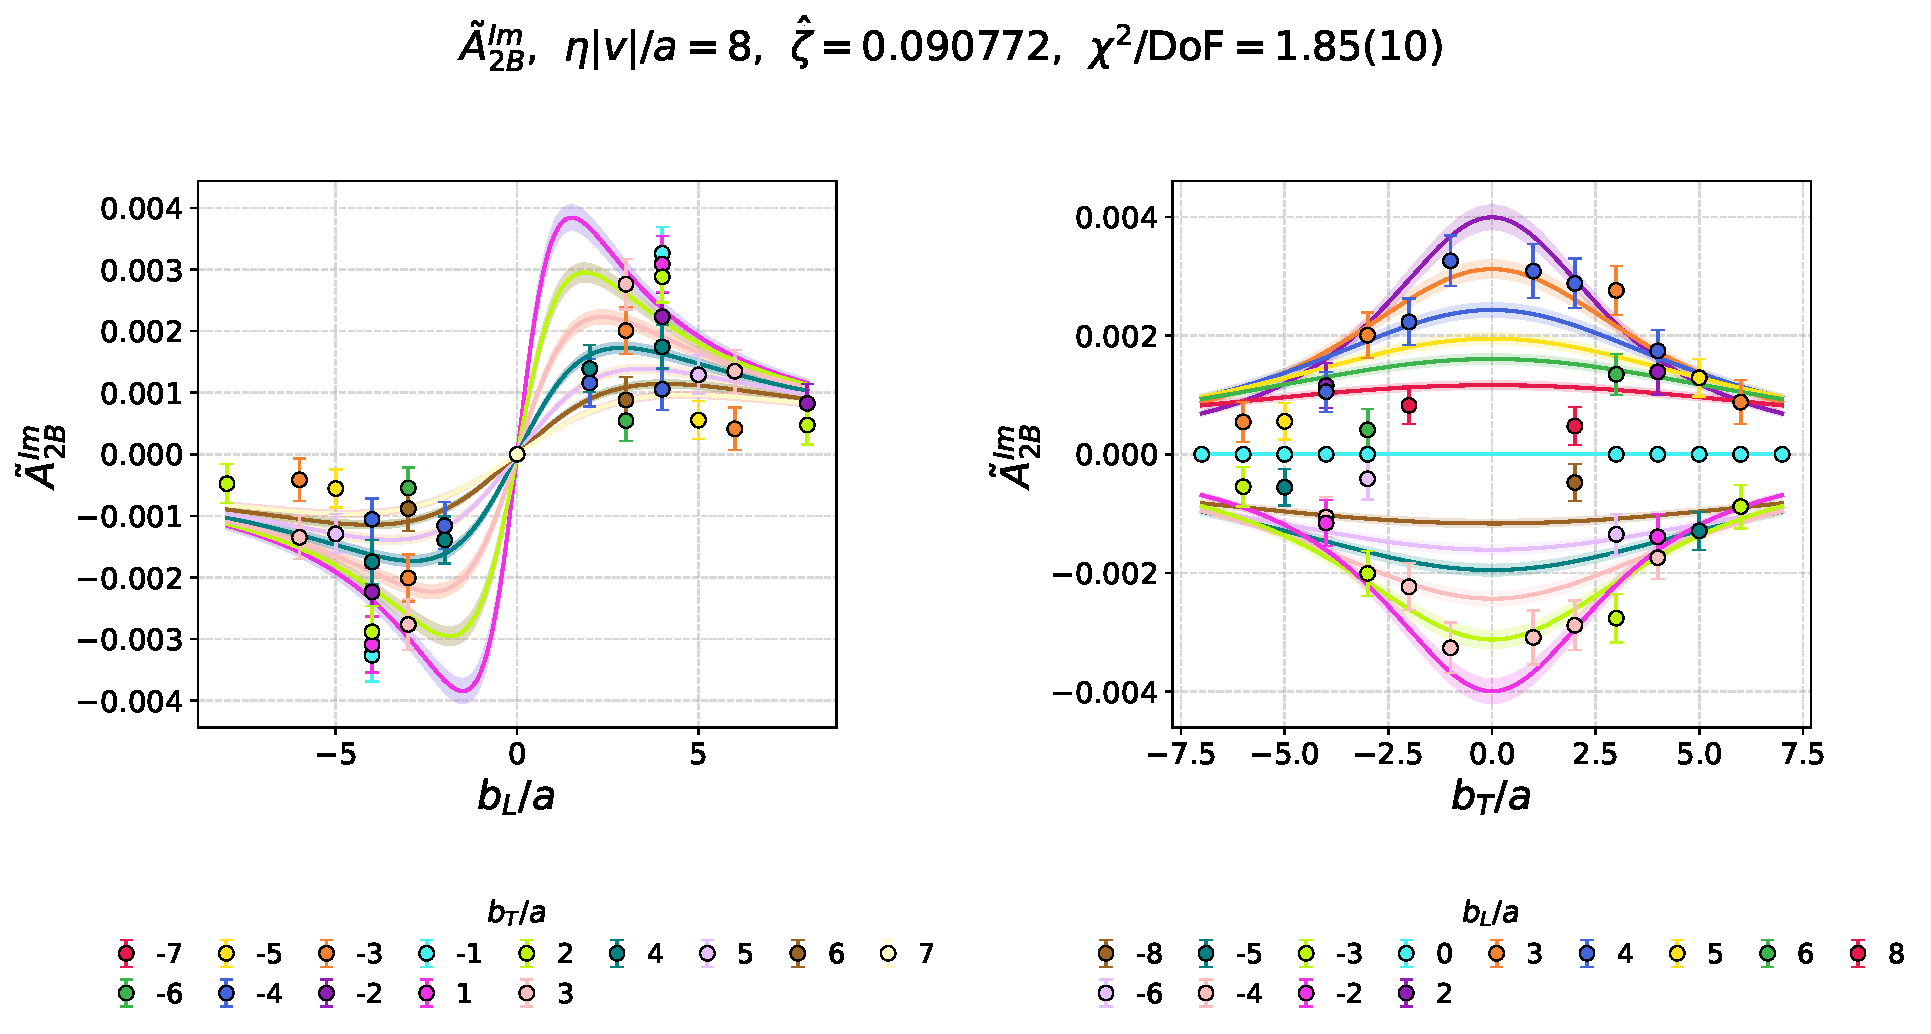
\includegraphics[width=\linewidth,height=.70\textheight,keepaspectratio]{fitting/ImA2B_eta8_PL-1_WithFit_2D.pdf}
\par\small Both spatial-coordinate slices. Same simultaneous fit, with Jackknife bands.

\figsrc{Thesis: plots; ImA2B\_eta8\_PL-1\_WithFit\_2D}
\end{frame}

\begin{frame}{Fixed staple $\eta=8$: $\tAmp_{2B}^{\mathrm{Im}}$, $P_L=-1$}
\centering
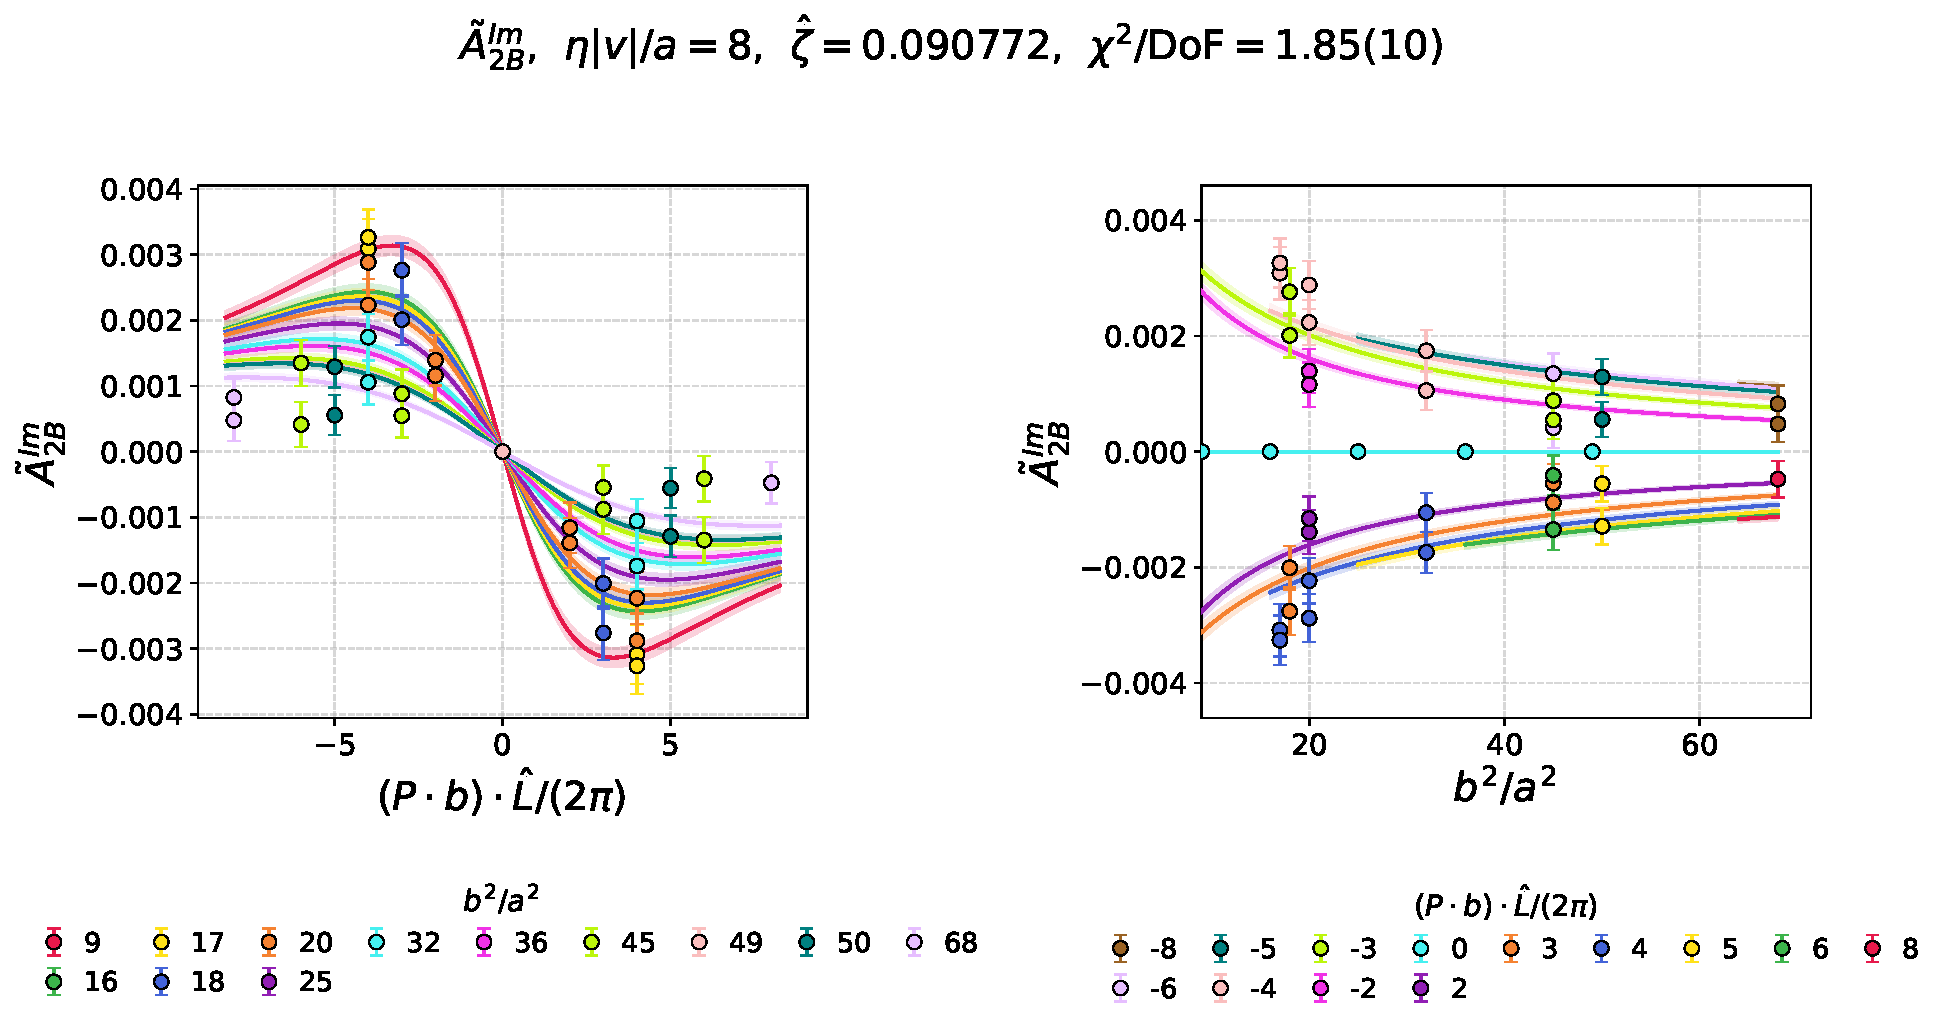
\includegraphics[width=\linewidth,height=.70\textheight,keepaspectratio]{fitting/ImA2B_Pb_bsq_eta8_PL-1_WithFit_2D.pdf}
\par\small Both invariant-coordinate slices. Same simultaneous fit, with Jackknife bands.

\figsrc{Thesis: plots; ImA2B\_Pb\_bsq\_eta8\_PL-1\_WithFit\_2D}
\end{frame}

\begin{frame}{Global fit: $\tAmp_{12B}^{\mathrm{Re}}$, $P_L=-1$}
\centering
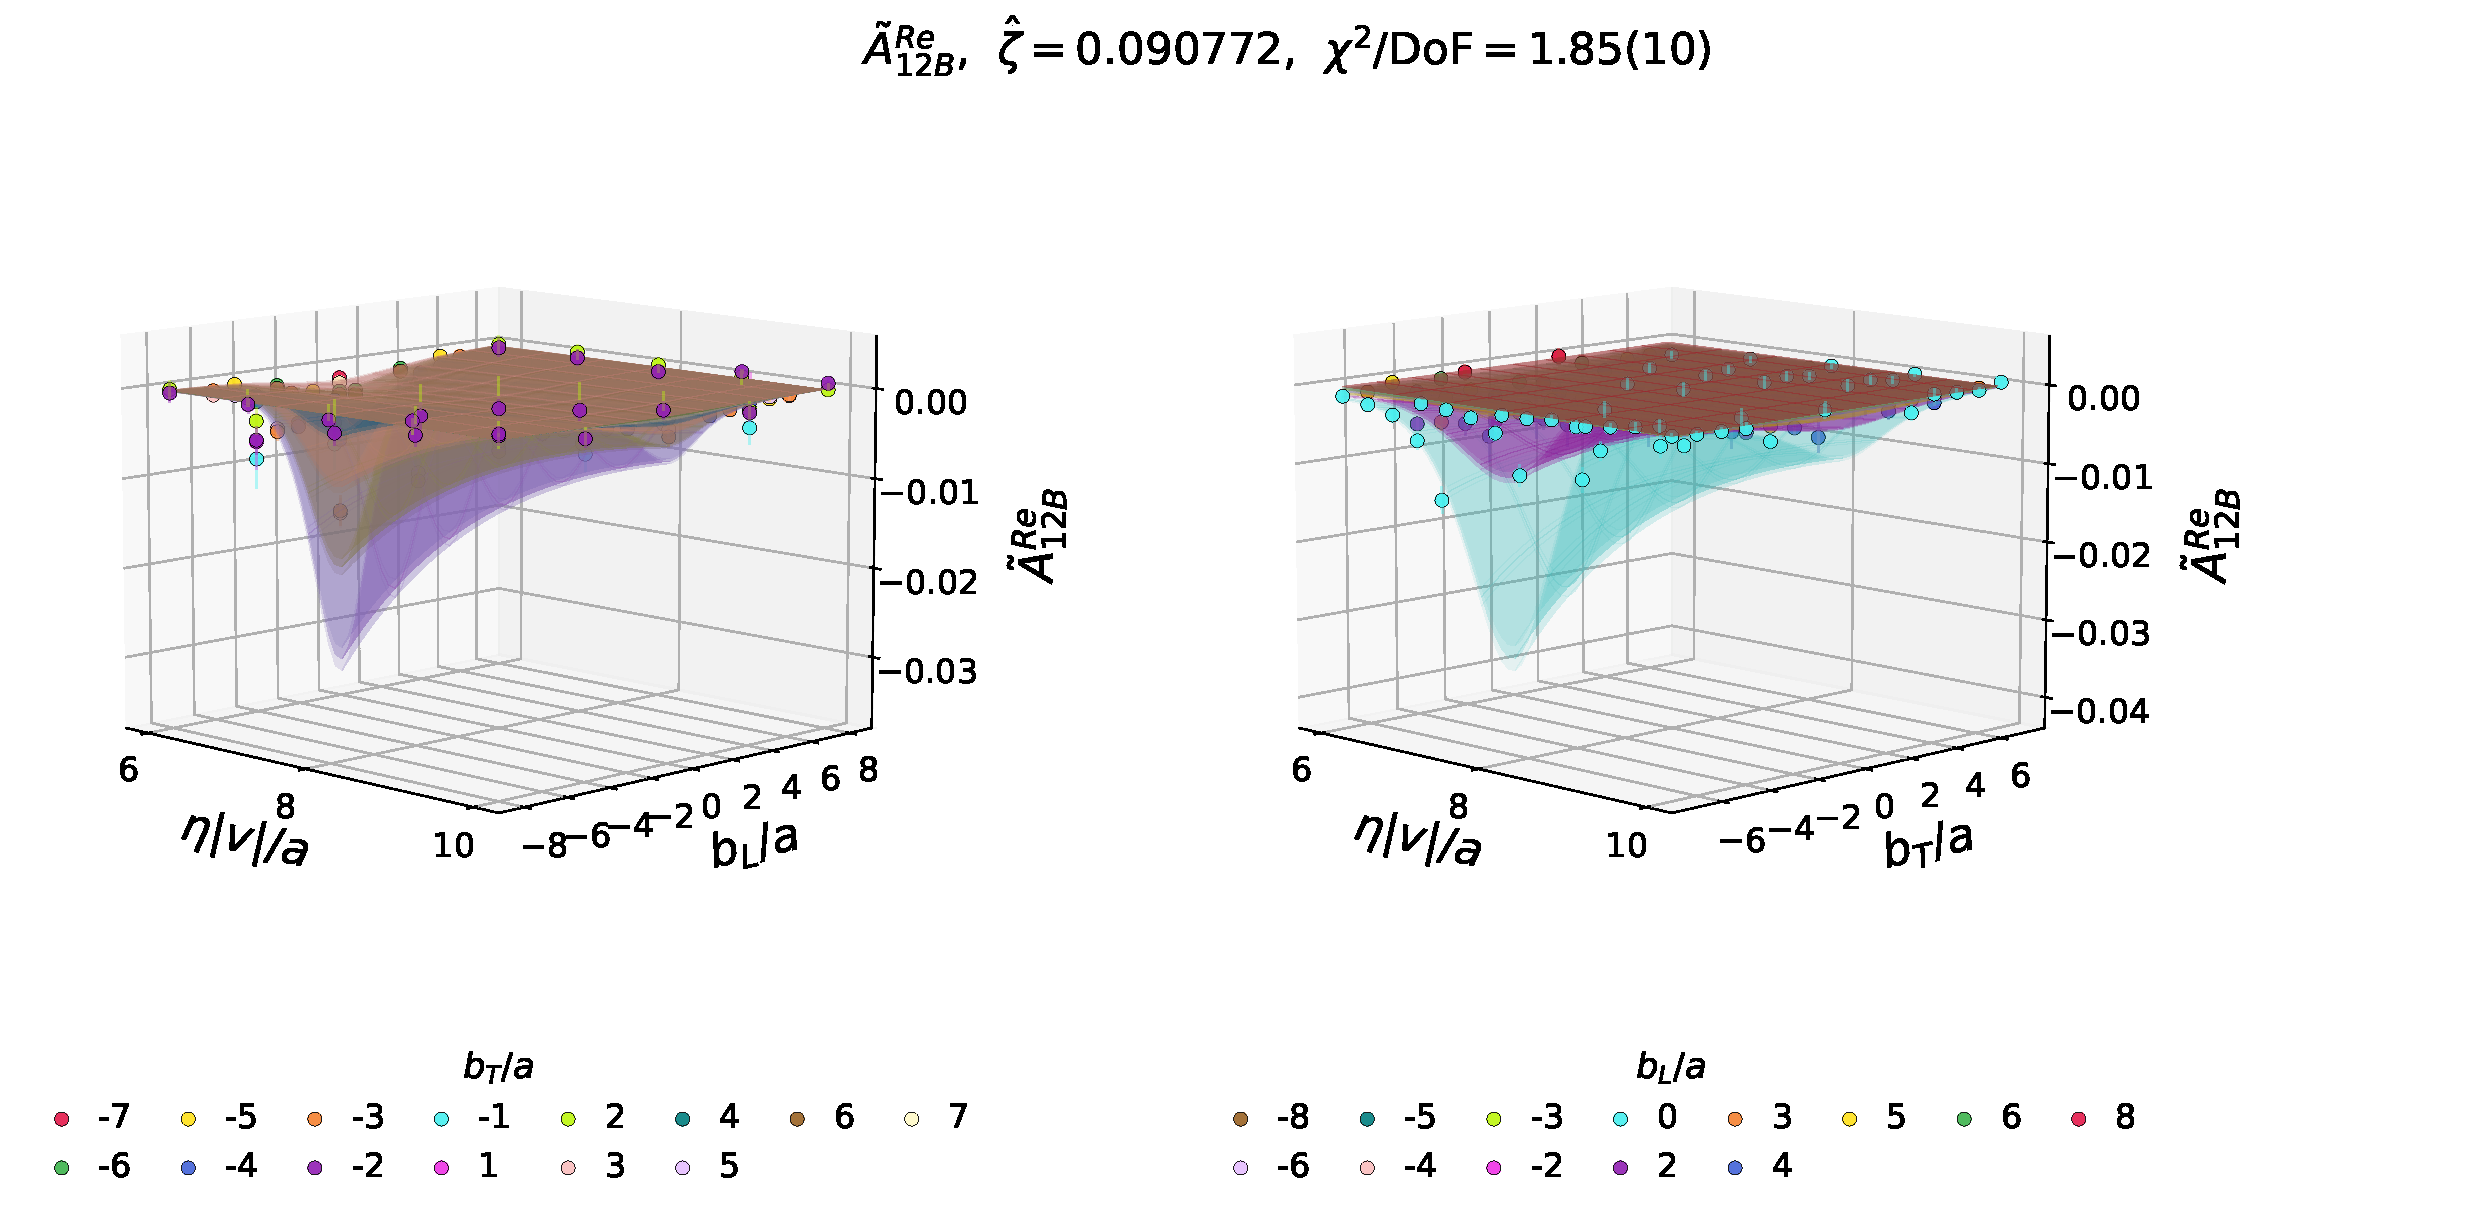
\includegraphics[width=\linewidth,height=.70\textheight,keepaspectratio]{fitting/ReA12B_PL-1_WithFit_3D.pdf}
\par\small Spatial coordinates: $(b_L,b_T,\eta)$. All panels and data overlays retained.

\figsrc{Thesis: plots; ReA12B\_PL-1\_WithFit\_3D}
\end{frame}

\begin{frame}{Global fit: $\tAmp_{12B}^{\mathrm{Re}}$, $P_L=-1$}
\centering
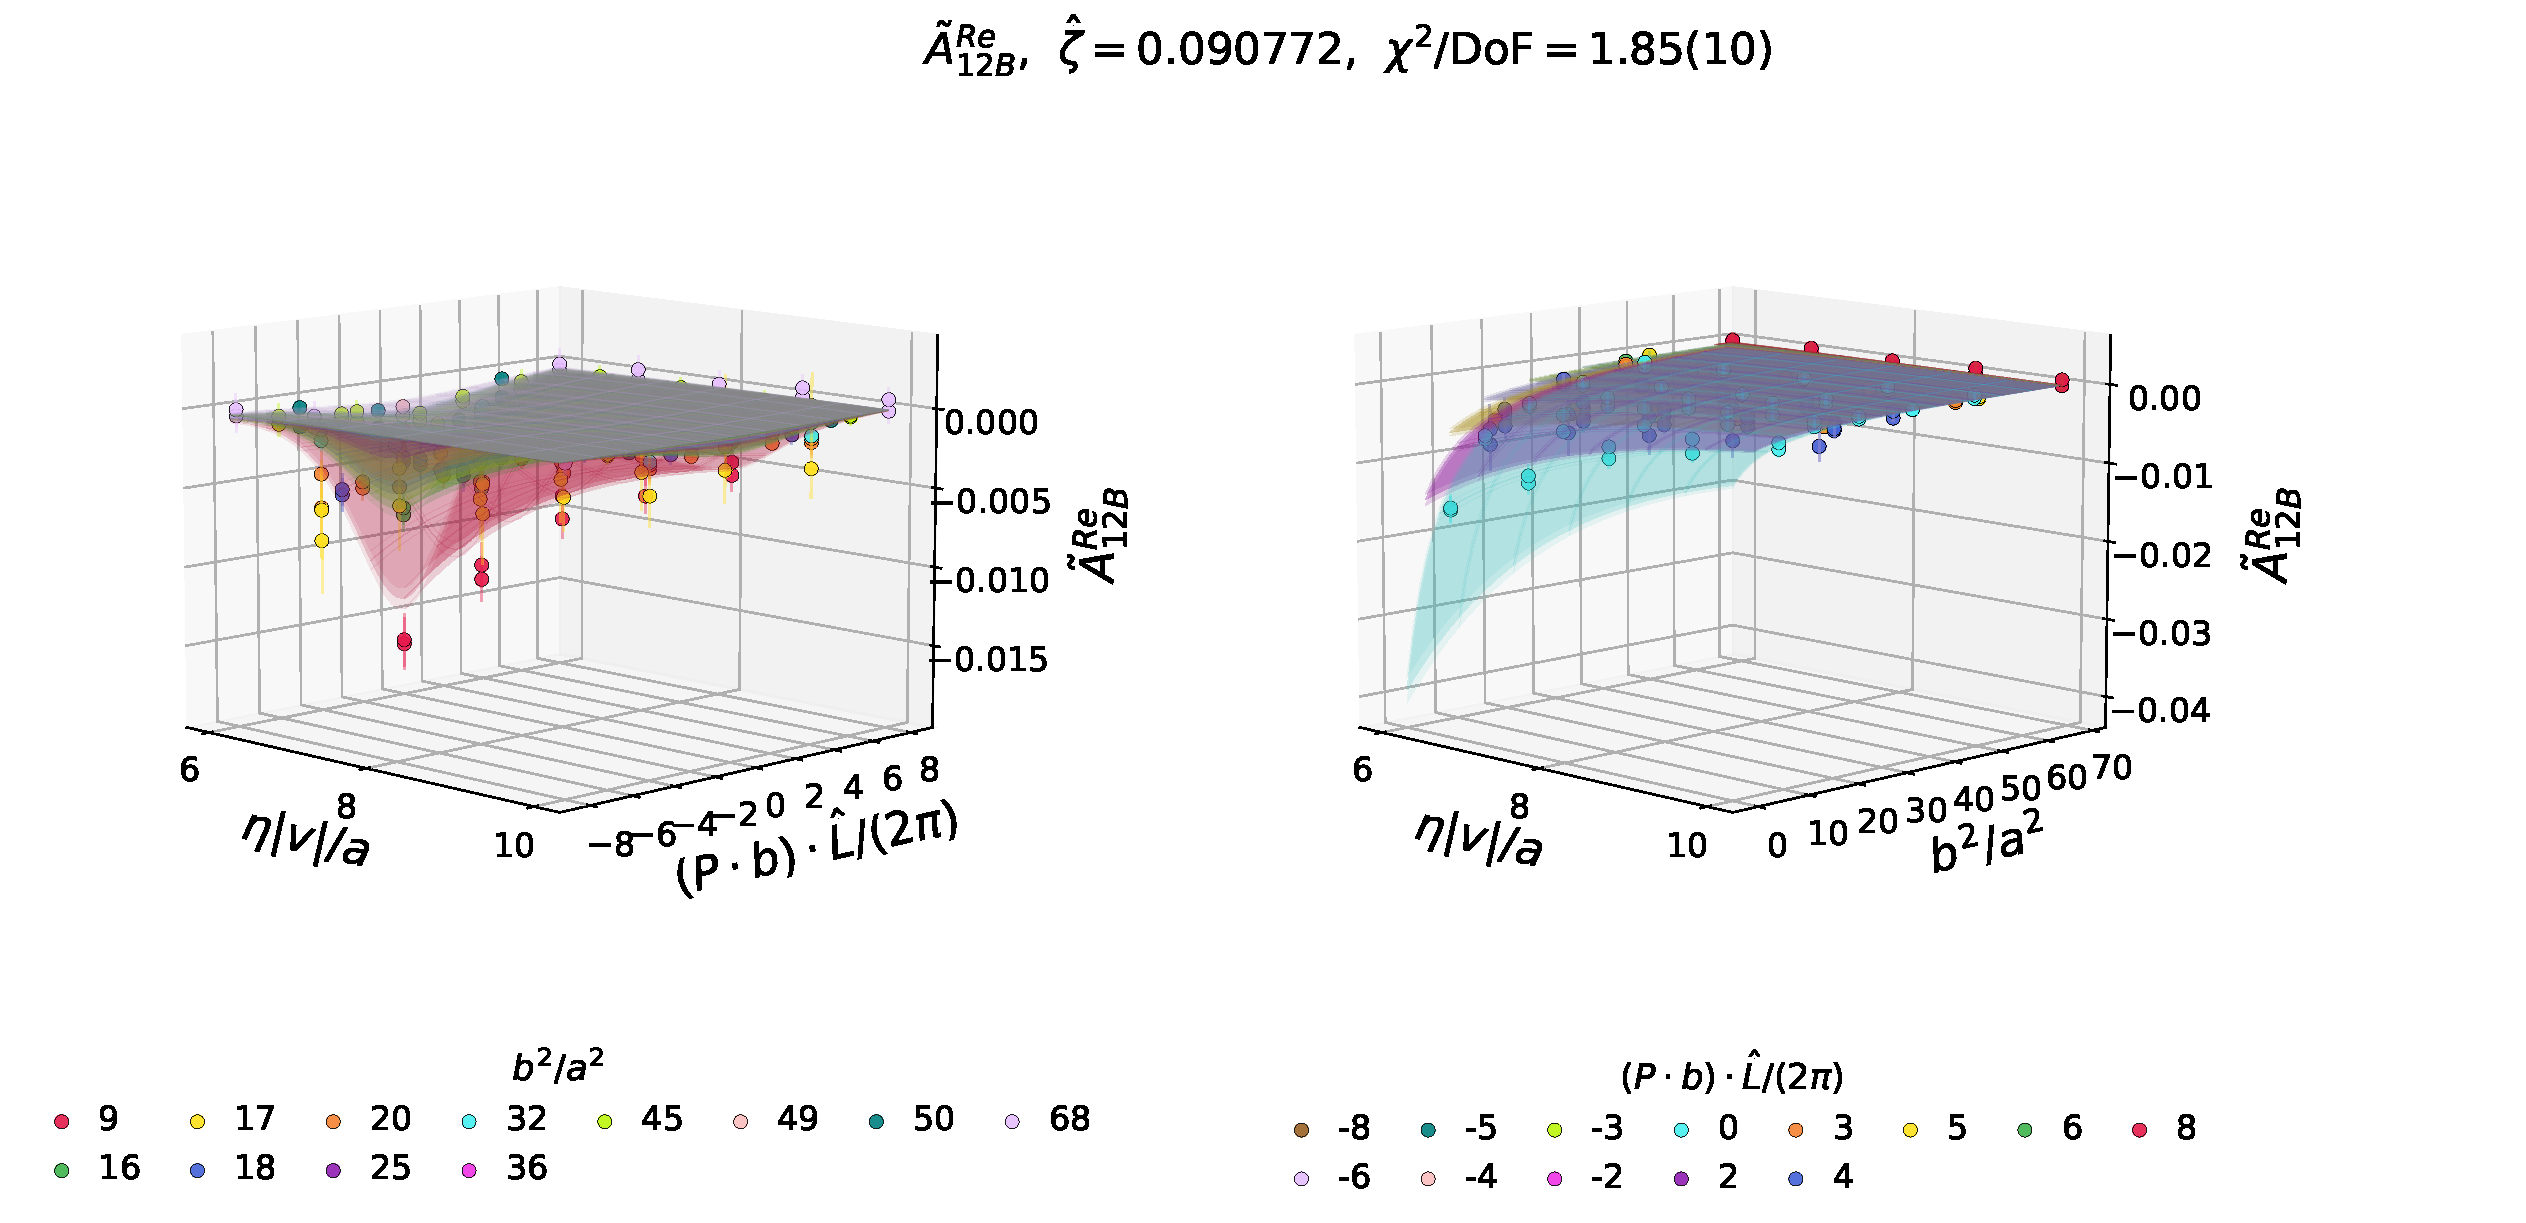
\includegraphics[width=\linewidth,height=.70\textheight,keepaspectratio]{fitting/ReA12B_Pb_bsq_PL-1_WithFit_3D.pdf}
\par\small Invariant coordinates: $(\nu,b^2,\eta)$. All panels and data overlays retained.

\figsrc{Thesis: plots; ReA12B\_Pb\_bsq\_PL-1\_WithFit\_3D}
\end{frame}

\begin{frame}{Fixed staple $\eta=8$: $\tAmp_{12B}^{\mathrm{Re}}$, $P_L=-1$}
\centering
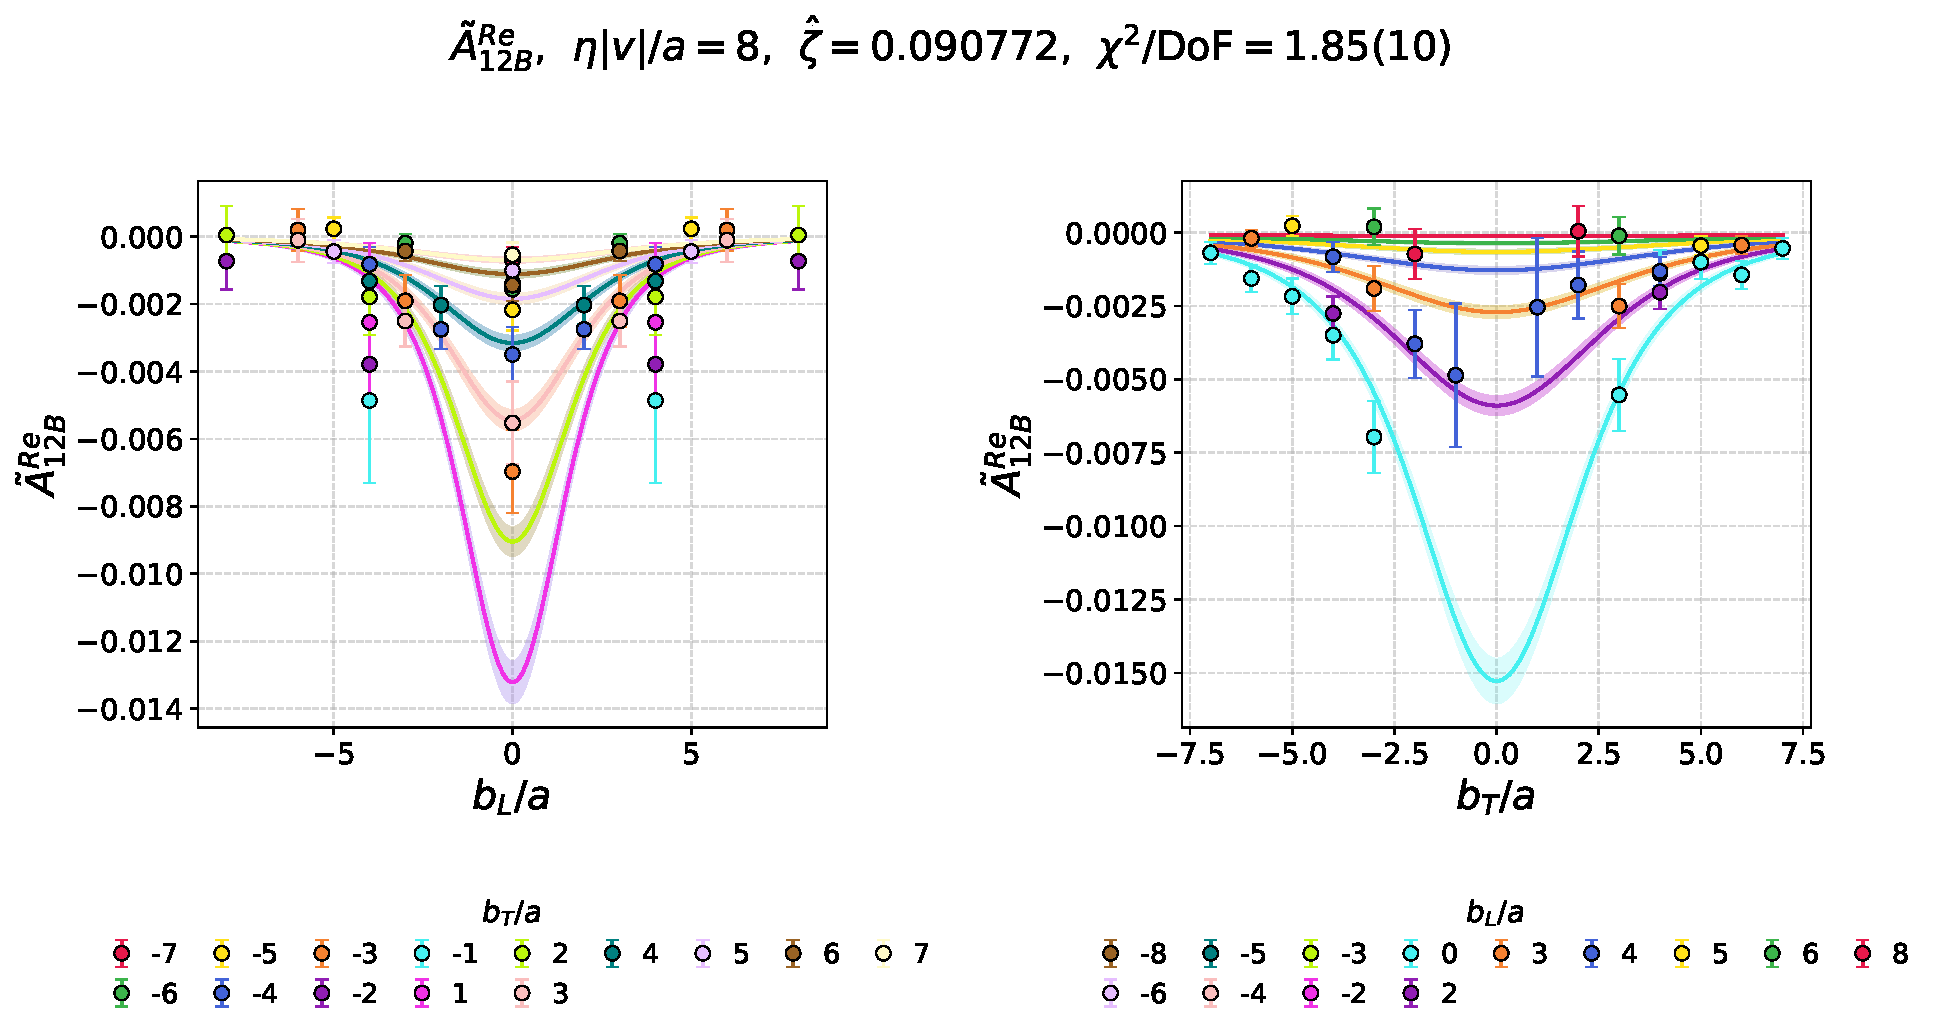
\includegraphics[width=\linewidth,height=.70\textheight,keepaspectratio]{fitting/ReA12B_eta8_PL-1_WithFit_2D.pdf}
\par\small Both spatial-coordinate slices. Same simultaneous fit, with Jackknife bands.

\figsrc{Thesis: plots; ReA12B\_eta8\_PL-1\_WithFit\_2D}
\end{frame}

\begin{frame}{Fixed staple $\eta=8$: $\tAmp_{12B}^{\mathrm{Re}}$, $P_L=-1$}
\centering
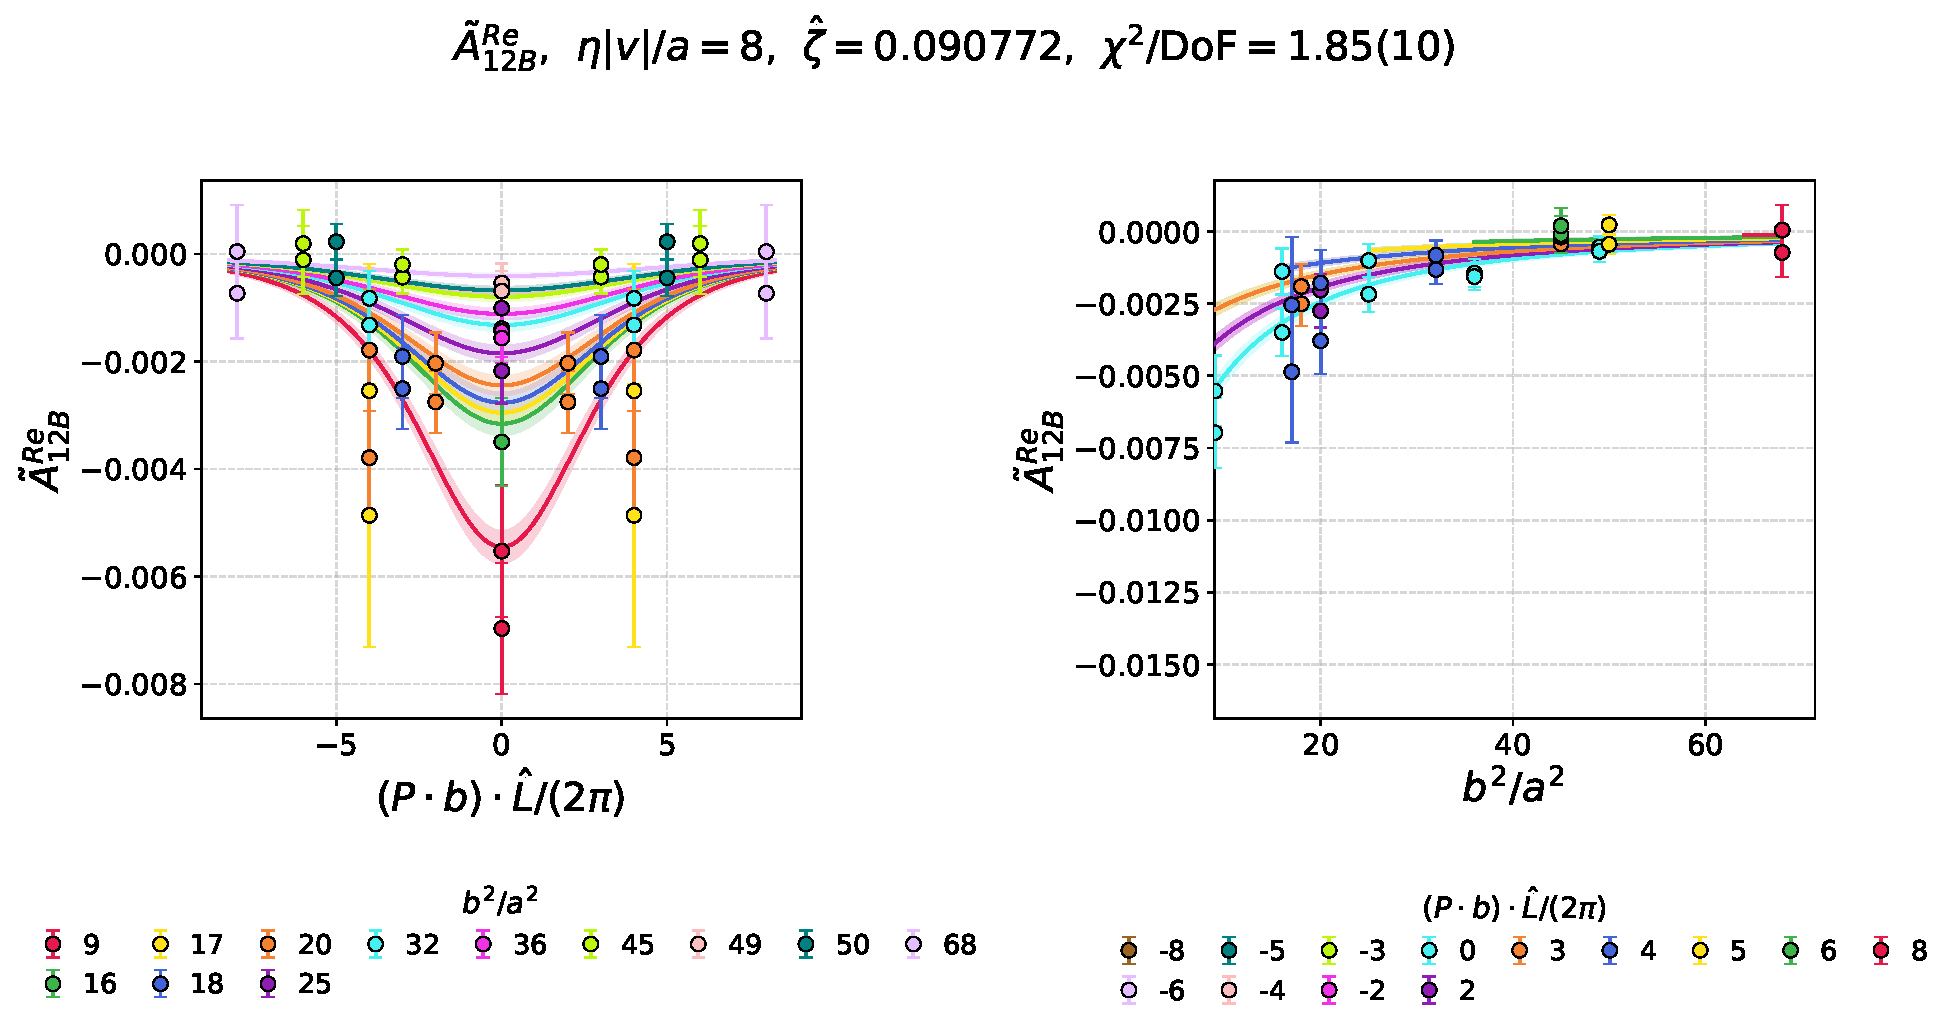
\includegraphics[width=\linewidth,height=.70\textheight,keepaspectratio]{fitting/ReA12B_Pb_bsq_eta8_PL-1_WithFit_2D.pdf}
\par\small Both invariant-coordinate slices. Same simultaneous fit, with Jackknife bands.

\figsrc{Thesis: plots; ReA12B\_Pb\_bsq\_eta8\_PL-1\_WithFit\_2D}
\end{frame}

\begin{frame}{Integrated Fourier results: $P_L=-1$}
\small\renewcommand{\arraystretch}{1.8}\begin{tabular}{lcccc}\toprule Integral & $(-\infty,\infty)$ & $[-1,1]$ & $[-1,0]$ & $[0,1]$\\\midrule
$\int dx\,E$ & 0.889(24) & 0.780(29) & 0.390(14) & 0.390(14) \\
$\int dx\,O$ & -1(108)e-17 & 2(282)e-17 & 0.1223(58) & -0.1223(58) \\
$\int dx\,\tilde f_1^{(0)}$ & 1.778(47) & 1.560(58) & 0.535(25) & 1.024(36) \\
$\int dx\,\tilde f_{1T}^{\perp(1)}$ & 0.469(23) & 0.454(23) & 0.227(12) & 0.227(12) \\
$m_N\int dx\,\tilde f_{1T}^{\perp(1)}/\int dx\,\tilde f_1^{(0)}$ & 0.284(14) & 0.313(18) & 0.456(29) & 0.238(13) \\
\bottomrule\end{tabular}\par\medskip $b^2=9a^2$; all values and Jackknife uncertainties retained. Numerical values retain the source normalization. The last row is in GeV.
\figsrc{Thesis: SimultaneousFitsCov/Integration\_Table\_PL-1\_bmin3\_b2-9.tex}
\end{frame}

\begin{frame}{Fourier results (2D): $P_L=-1$, unpolarized}
\centering
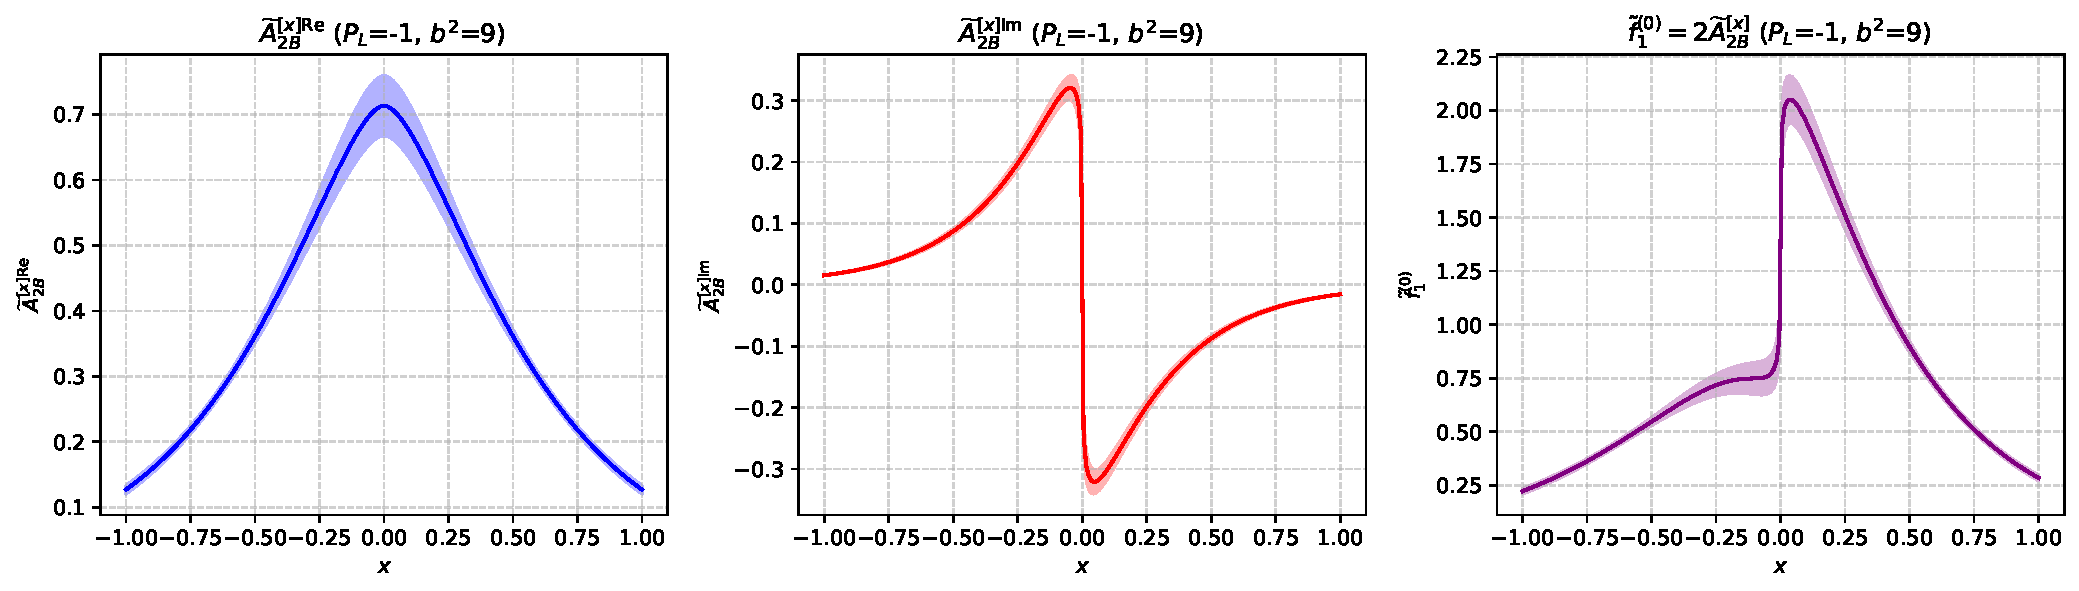
\includegraphics[width=\linewidth,height=.70\textheight,keepaspectratio]{fitting/FT_xdep_A2B_A12B_bmin3_eta610_b2-9_PL-1__row1.pdf}
\par\small Even, odd, and unpolarized transforms. Fixed $b^2=9a^2$.

\figsrc{Thesis: SimultaneousFitsCov; FT\_xdep\_A2B\_A12B\_bmin3\_eta610\_b2-9\_PL-1}
\end{frame}

\begin{frame}{Fourier results (2D): $P_L=-1$, Sivers}
\centering
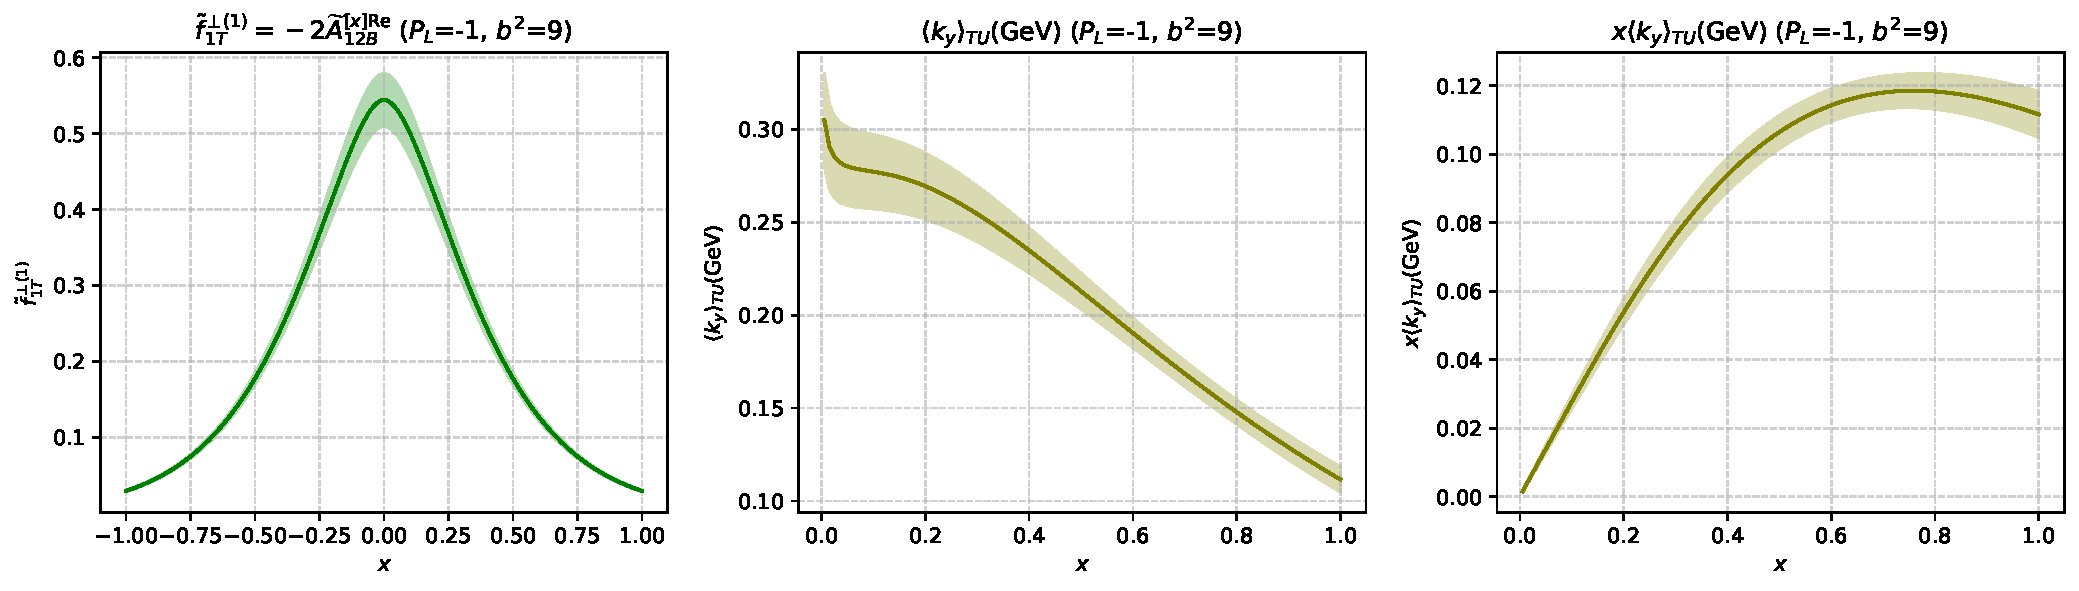
\includegraphics[width=\linewidth,height=.70\textheight,keepaspectratio]{fitting/FT_xdep_A2B_A12B_bmin3_eta610_b2-9_PL-1__row2.pdf}
\par\small Sivers transform, shift, and $x\langle k_y\rangle_{TU}$. Fixed $b^2=9a^2$.

\figsrc{Thesis: SimultaneousFitsCov; FT\_xdep\_A2B\_A12B\_bmin3\_eta610\_b2-9\_PL-1}
\end{frame}

\begin{frame}{Fourier results (3D): $P_L=-1$, unpolarized}
\centering
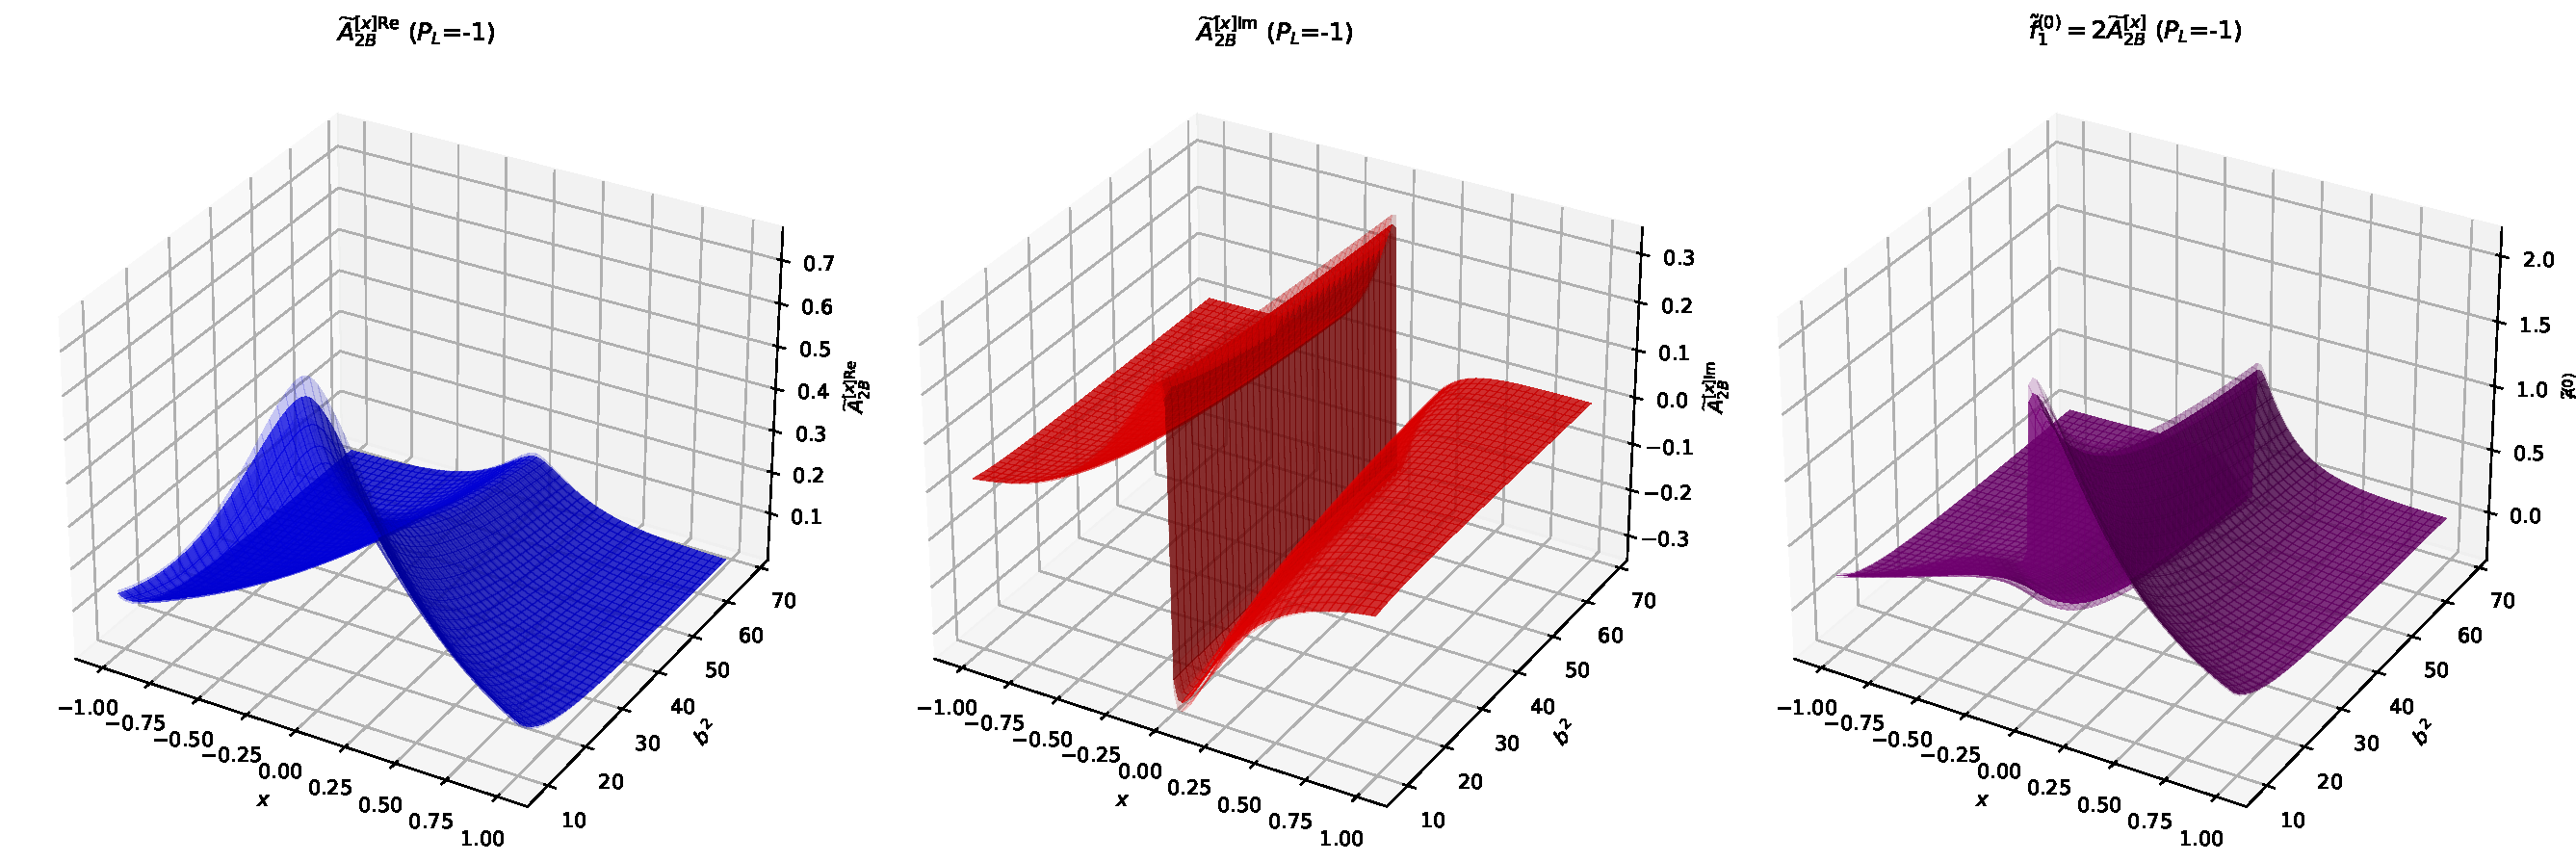
\includegraphics[width=\linewidth,height=.70\textheight,keepaspectratio]{fitting/FT_xdep_3D_A2B_A12B_bmin3_eta610_PL-1__row1.pdf}
\par\small Even, odd, and unpolarized transforms. Full $b^2/a^2\in[9,68]$ dependence.

\figsrc{Thesis: SimultaneousFitsCov; FT\_xdep\_3D\_A2B\_A12B\_bmin3\_eta610\_PL-1}
\end{frame}

\begin{frame}{Fourier results (3D): $P_L=-1$, Sivers}
\centering
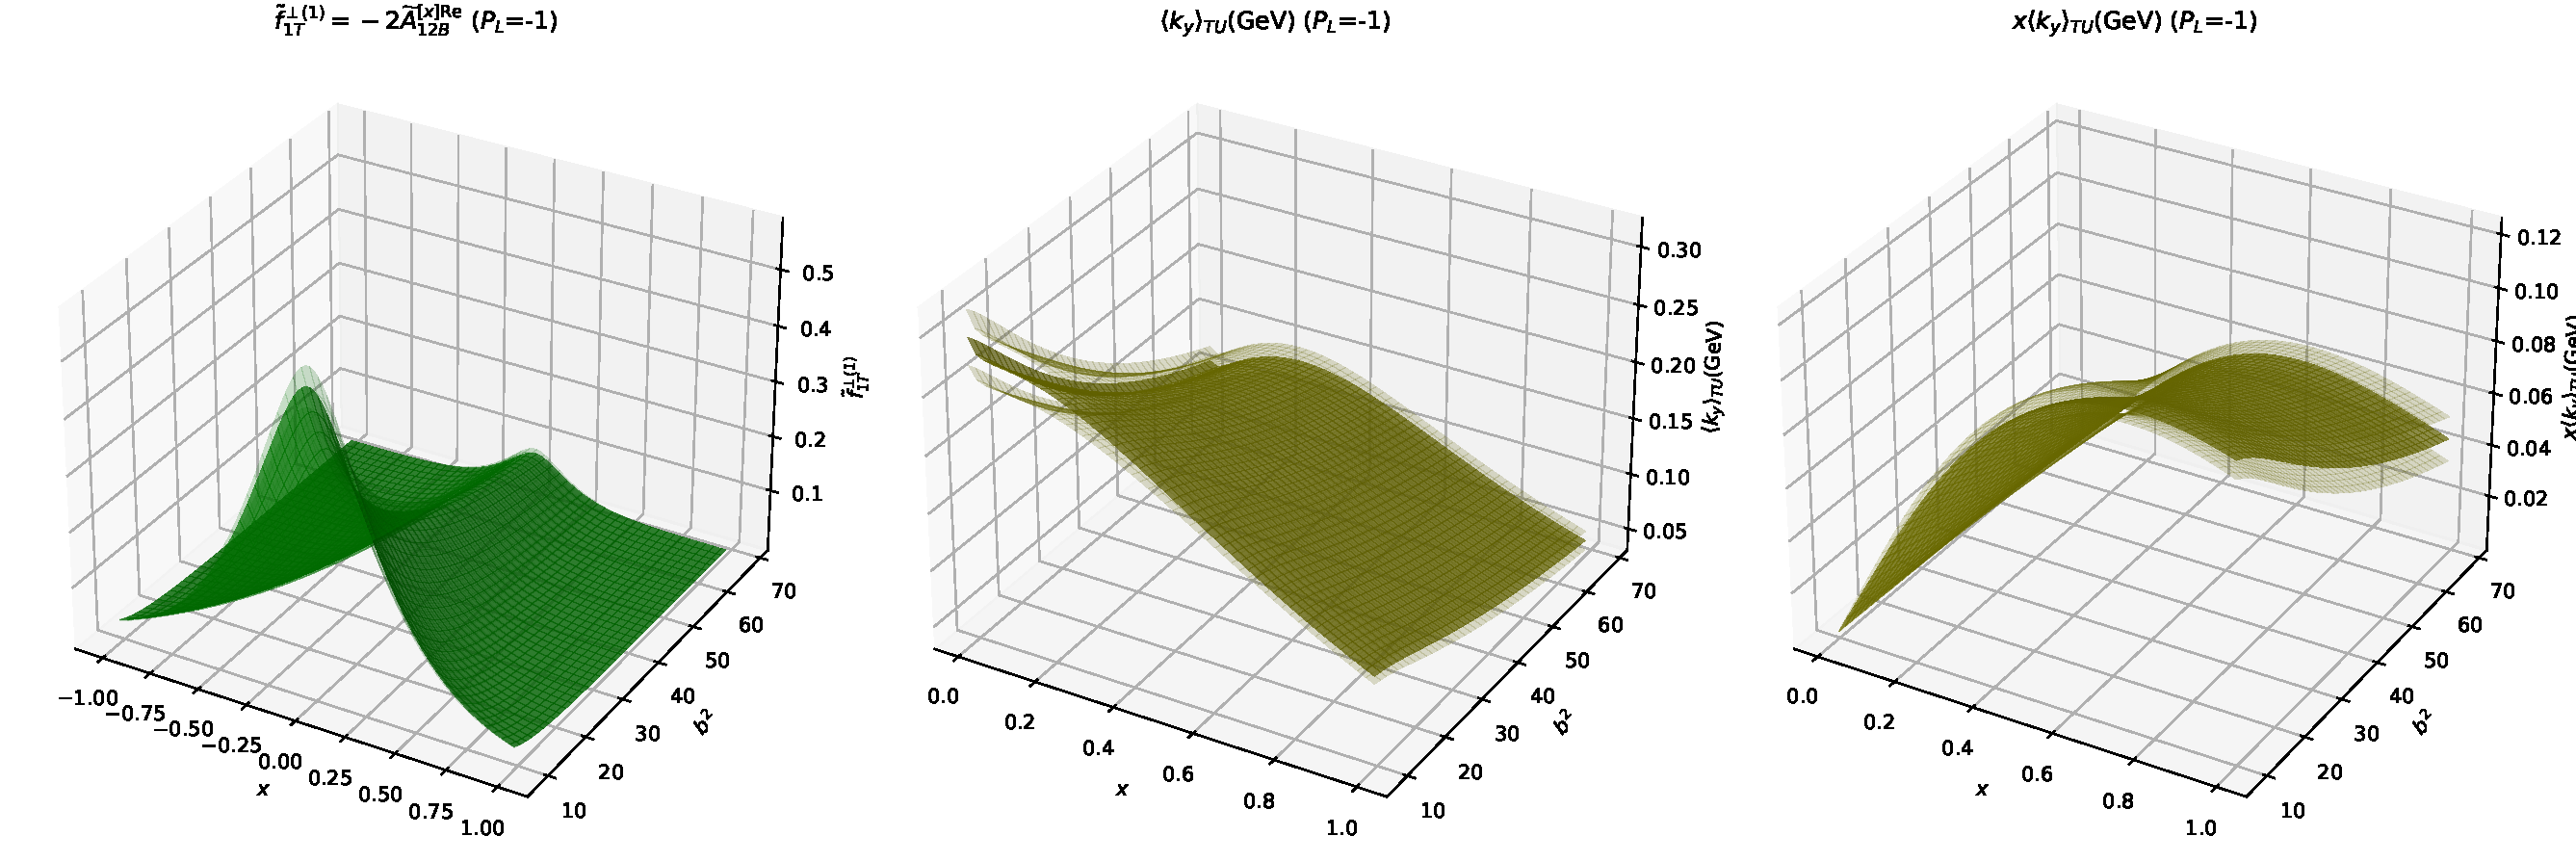
\includegraphics[width=\linewidth,height=.70\textheight,keepaspectratio]{fitting/FT_xdep_3D_A2B_A12B_bmin3_eta610_PL-1__row2.pdf}
\par\small Sivers transform, shift, and $x\langle k_y\rangle_{TU}$. Full $b^2/a^2\in[9,68]$ dependence.

\figsrc{Thesis: SimultaneousFitsCov; FT\_xdep\_3D\_A2B\_A12B\_bmin3\_eta610\_PL-1}
\end{frame}

\begin{frame}{Simultaneous fit parameters: $P_L=-2$}
\small $|\vect b|\ge3a$, $6\le\eta\le10$; reported $\chi^2_{\rm aug}/N_{\rm data}=1.197(85)$.\par\medskip
\begin{columns}[t]\begin{column}{.32\textwidth}\centering $\tAmp_{2B}^{\mathrm{Re}}$\par\medskip\renewcommand{\arraystretch}{1.3}\begin{tabular}{cc}\toprule Parameter & Value\\\midrule
$a$ & $3.9833(80)$ \\
$c$ & $0.166(35)$ \\
$d$ & $0.1020(46)$ \\
$k_1$ & $12.305(14)$ \\
$k_2$ & $-36.1919(27)$ \\
$j$ & $2.061(20)$ \\
$f$ & $0.5357(66)$ \\\bottomrule\end{tabular}\end{column}\begin{column}{.32\textwidth}\centering $\tAmp_{2B}^{\mathrm{Im}}$\par\medskip\renewcommand{\arraystretch}{1.3}\begin{tabular}{cc}\toprule Parameter & Value\\\midrule
$a''$ & $0.368(12)$ \\
$c''$ & $0.1346(69)$ \\
$d''$ & $0.1305(67)$ \\
$j''$ & $1.141(20)$ \\
$f$ & $0.5357(66)$ \\\bottomrule\end{tabular}\end{column}\begin{column}{.32\textwidth}\centering $\tAmp_{12B}^{\mathrm{Re}}$\par\medskip\renewcommand{\arraystretch}{1.3}\begin{tabular}{cc}\toprule Parameter & Value\\\midrule
$a'$ & $0.632(19)$ \\
$c'$ & $0.0769(54)$ \\
$d'$ & $0.0741(52)$ \\
$j'$ & $2.0141(69)$ \\
$f$ & $0.5357(66)$ \\\bottomrule\end{tabular}\end{column}\end{columns}
\figsrc{Thesis: SimultaneousFitsCov/Fit\_Table\_PL-2\_bmin3.tex}
\end{frame}

\begin{frame}{Global fit: $\tAmp_{2B}^{\mathrm{Re}}$, $P_L=-2$}
\centering
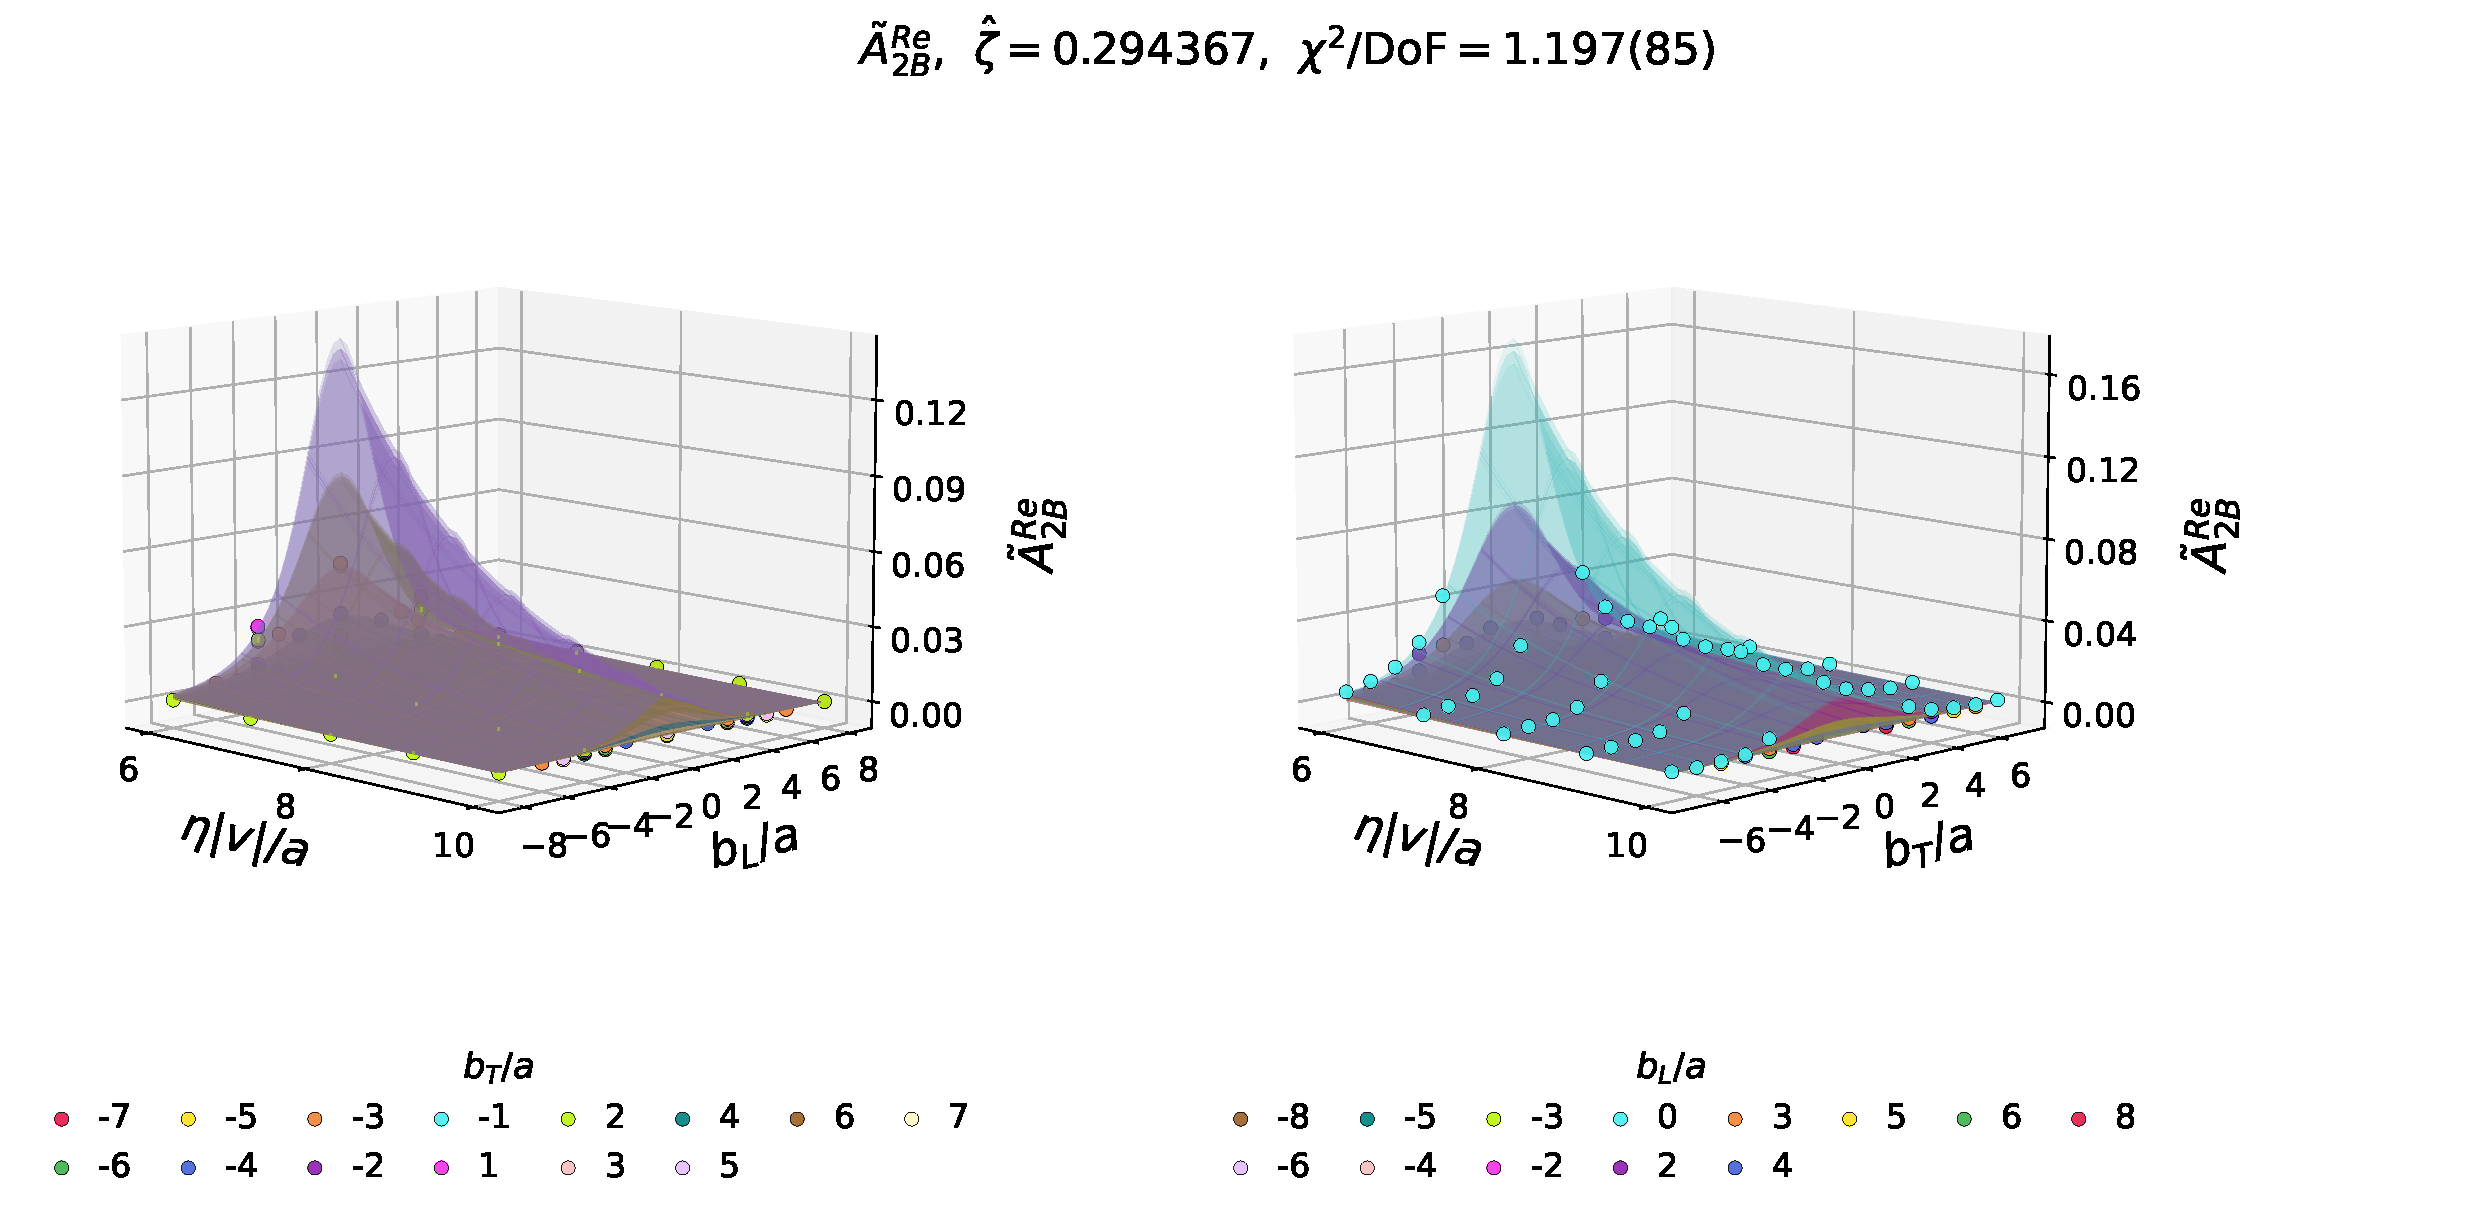
\includegraphics[width=\linewidth,height=.70\textheight,keepaspectratio]{fitting/ReA2B_PL-2_WithFit_3D.pdf}
\par\small Spatial coordinates: $(b_L,b_T,\eta)$. All panels and data overlays retained.

\figsrc{Thesis: plots; ReA2B\_PL-2\_WithFit\_3D}
\end{frame}

\begin{frame}{Global fit: $\tAmp_{2B}^{\mathrm{Re}}$, $P_L=-2$}
\centering
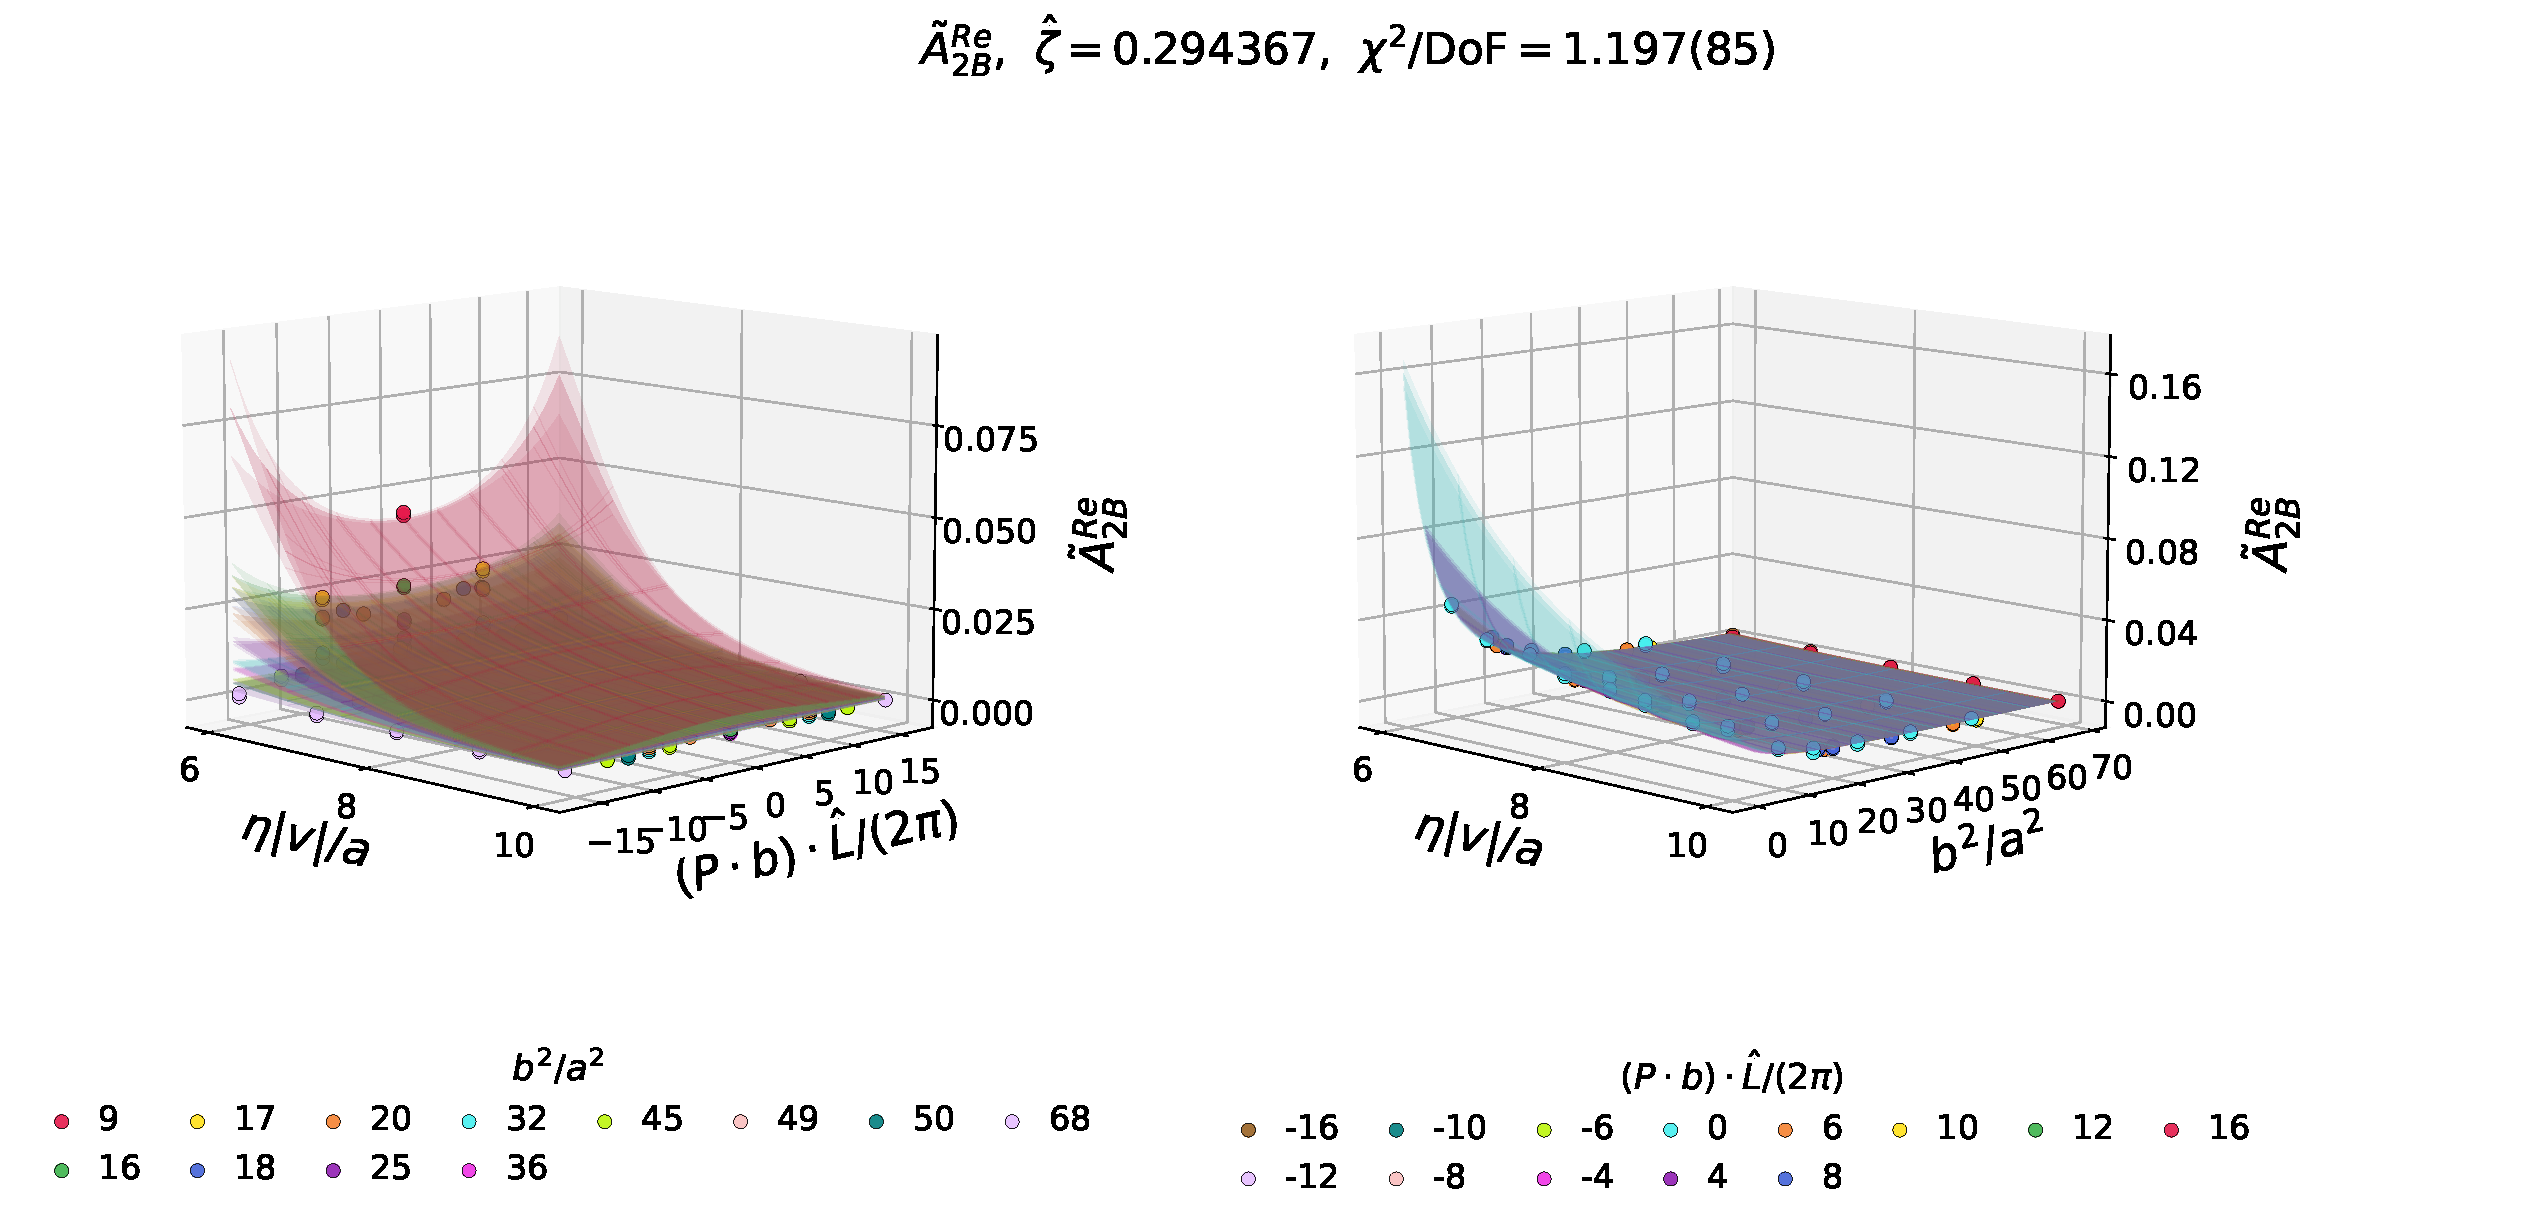
\includegraphics[width=\linewidth,height=.70\textheight,keepaspectratio]{fitting/ReA2B_Pb_bsq_PL-2_WithFit_3D.pdf}
\par\small Invariant coordinates: $(\nu,b^2,\eta)$. All panels and data overlays retained.

\figsrc{Thesis: plots; ReA2B\_Pb\_bsq\_PL-2\_WithFit\_3D}
\end{frame}

\begin{frame}{Fixed staple $\eta=8$: $\tAmp_{2B}^{\mathrm{Re}}$, $P_L=-2$}
\centering
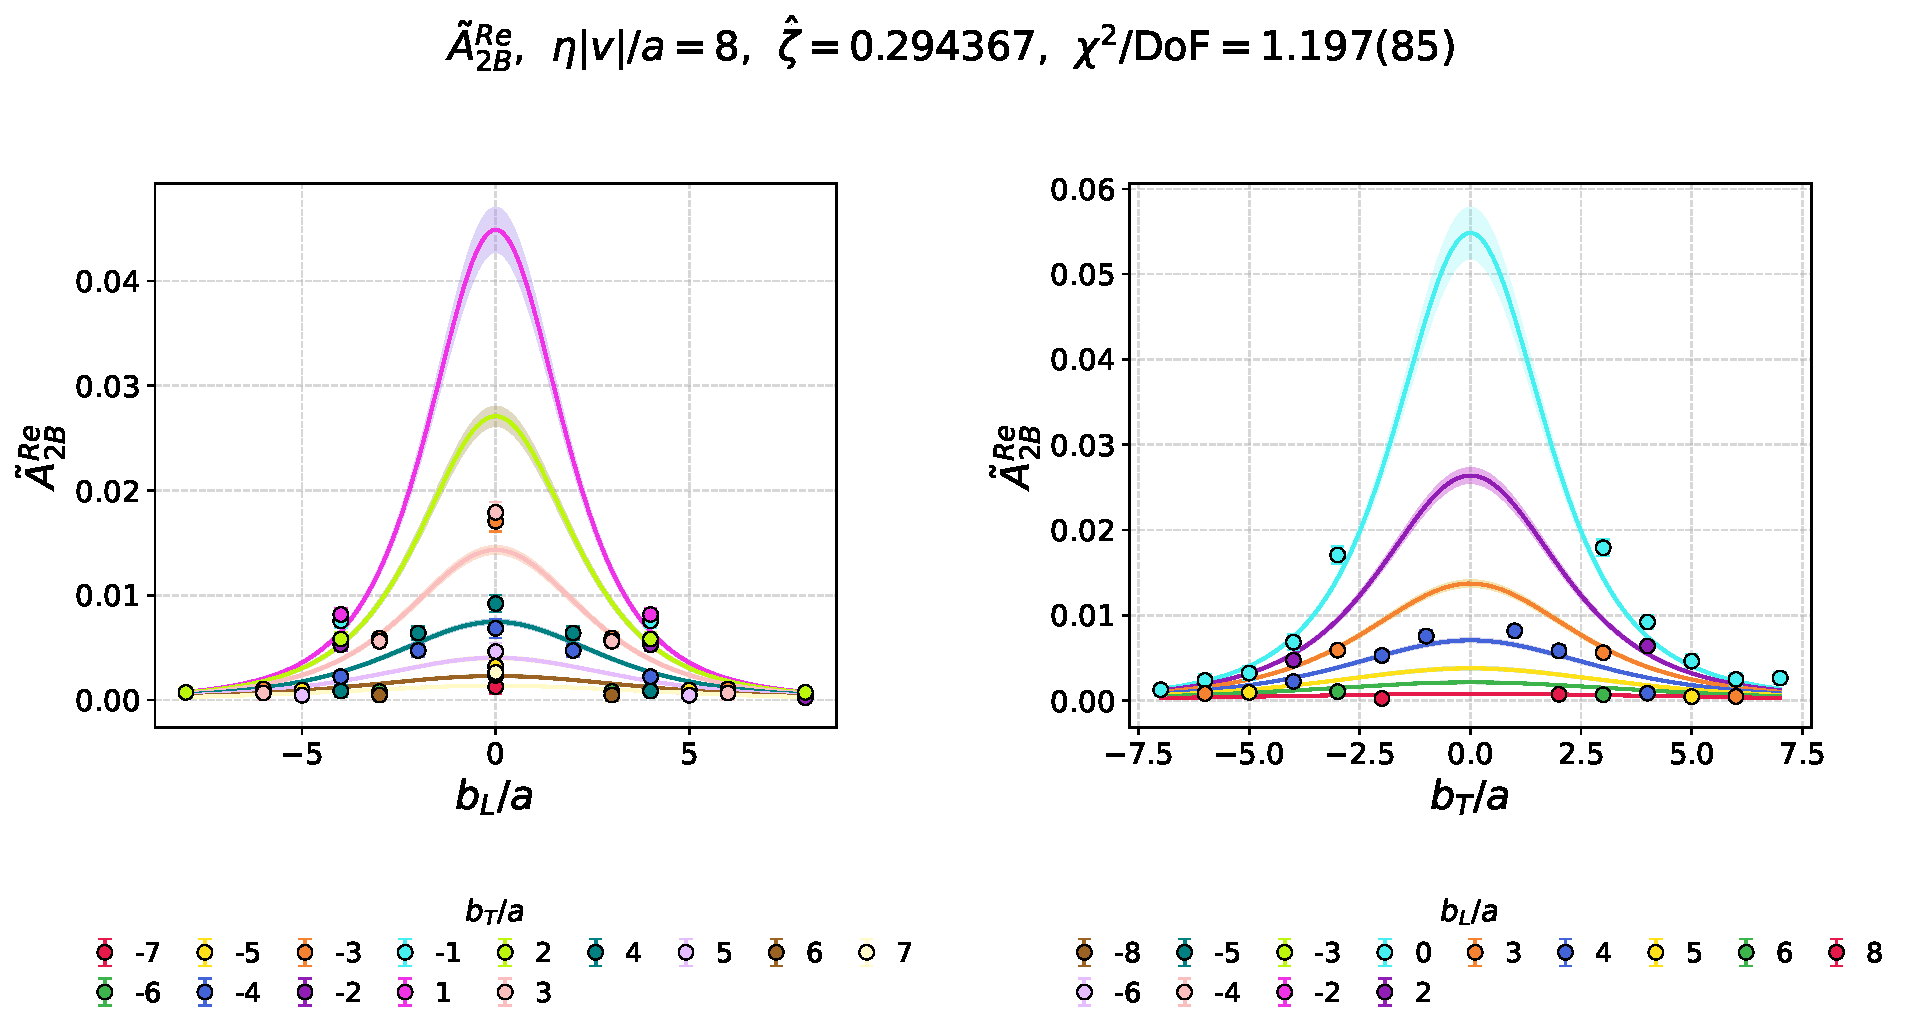
\includegraphics[width=\linewidth,height=.70\textheight,keepaspectratio]{fitting/ReA2B_eta8_PL-2_WithFit_2D.pdf}
\par\small Both spatial-coordinate slices. Same simultaneous fit, with Jackknife bands.

\figsrc{Thesis: plots; ReA2B\_eta8\_PL-2\_WithFit\_2D}
\end{frame}

\begin{frame}{Fixed staple $\eta=8$: $\tAmp_{2B}^{\mathrm{Re}}$, $P_L=-2$}
\centering
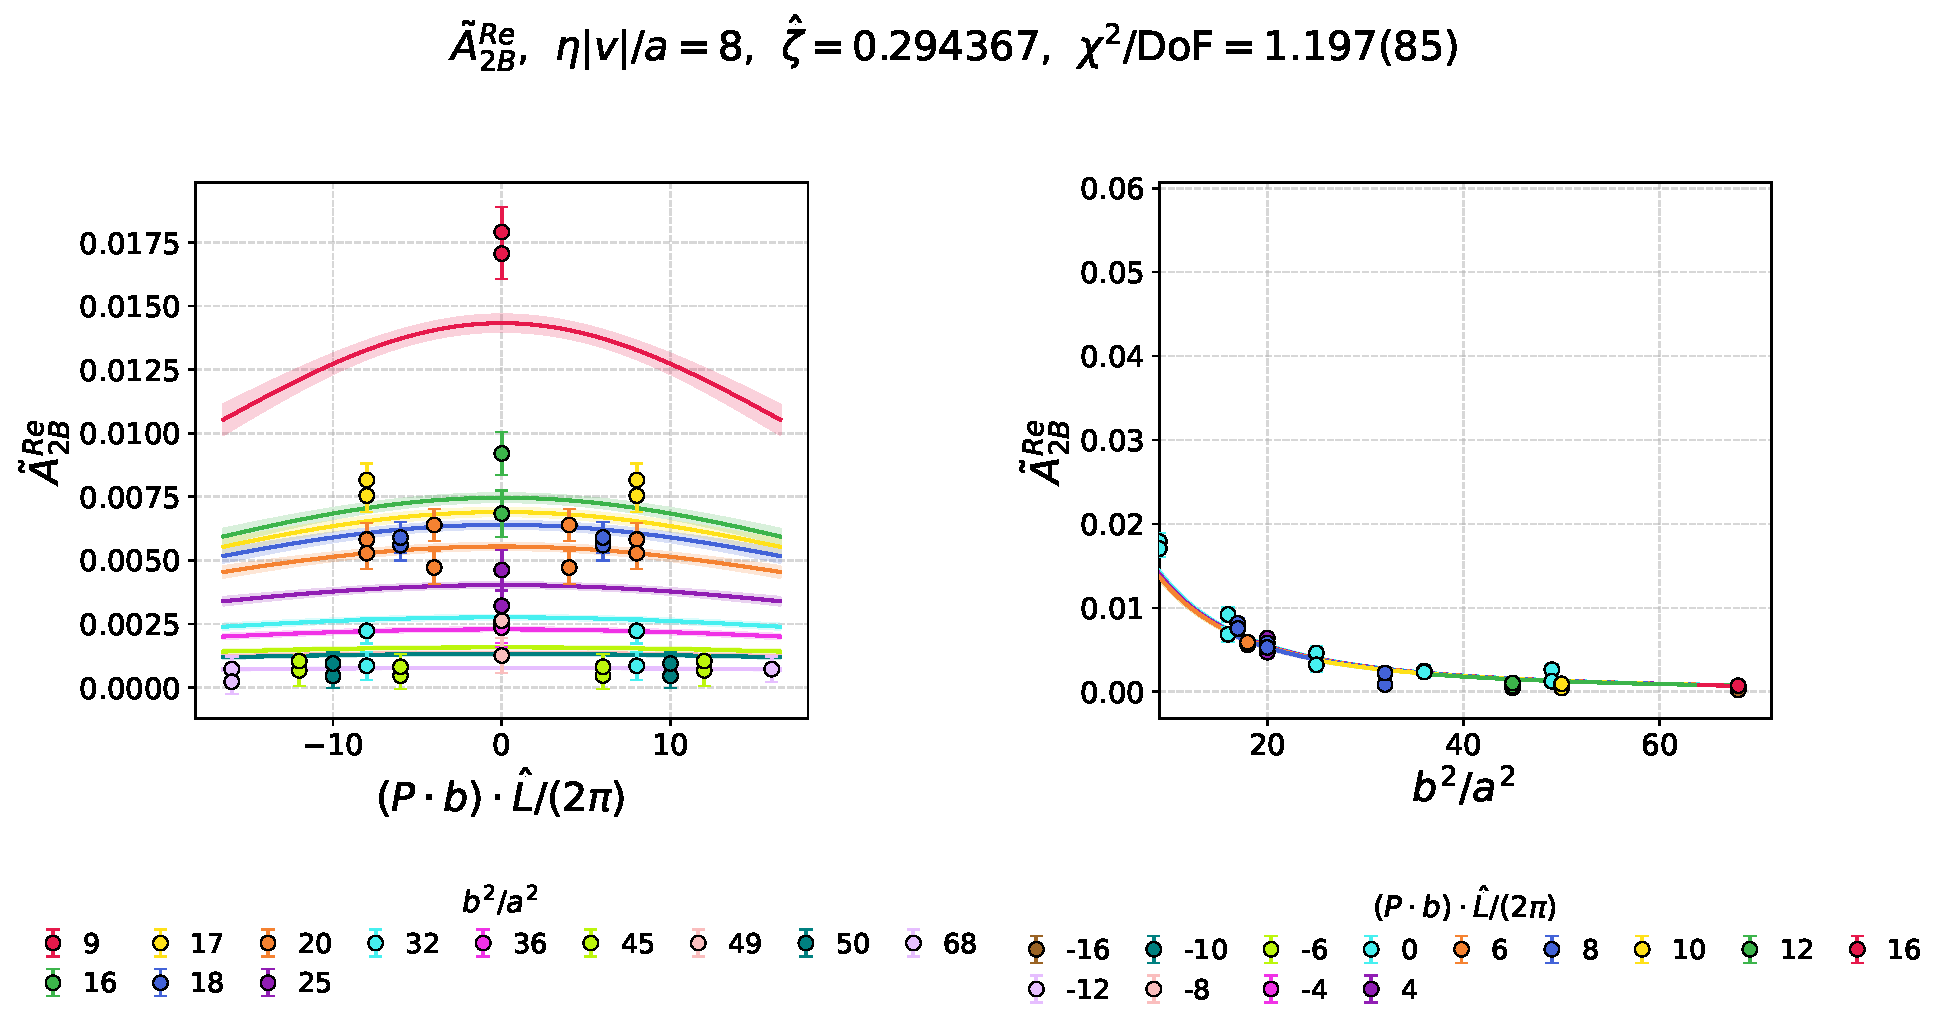
\includegraphics[width=\linewidth,height=.70\textheight,keepaspectratio]{fitting/ReA2B_Pb_bsq_eta8_PL-2_WithFit_2D.pdf}
\par\small Both invariant-coordinate slices. Same simultaneous fit, with Jackknife bands.

\figsrc{Thesis: plots; ReA2B\_Pb\_bsq\_eta8\_PL-2\_WithFit\_2D}
\end{frame}

\begin{frame}{Global fit: $\tAmp_{2B}^{\mathrm{Im}}$, $P_L=-2$}
\centering
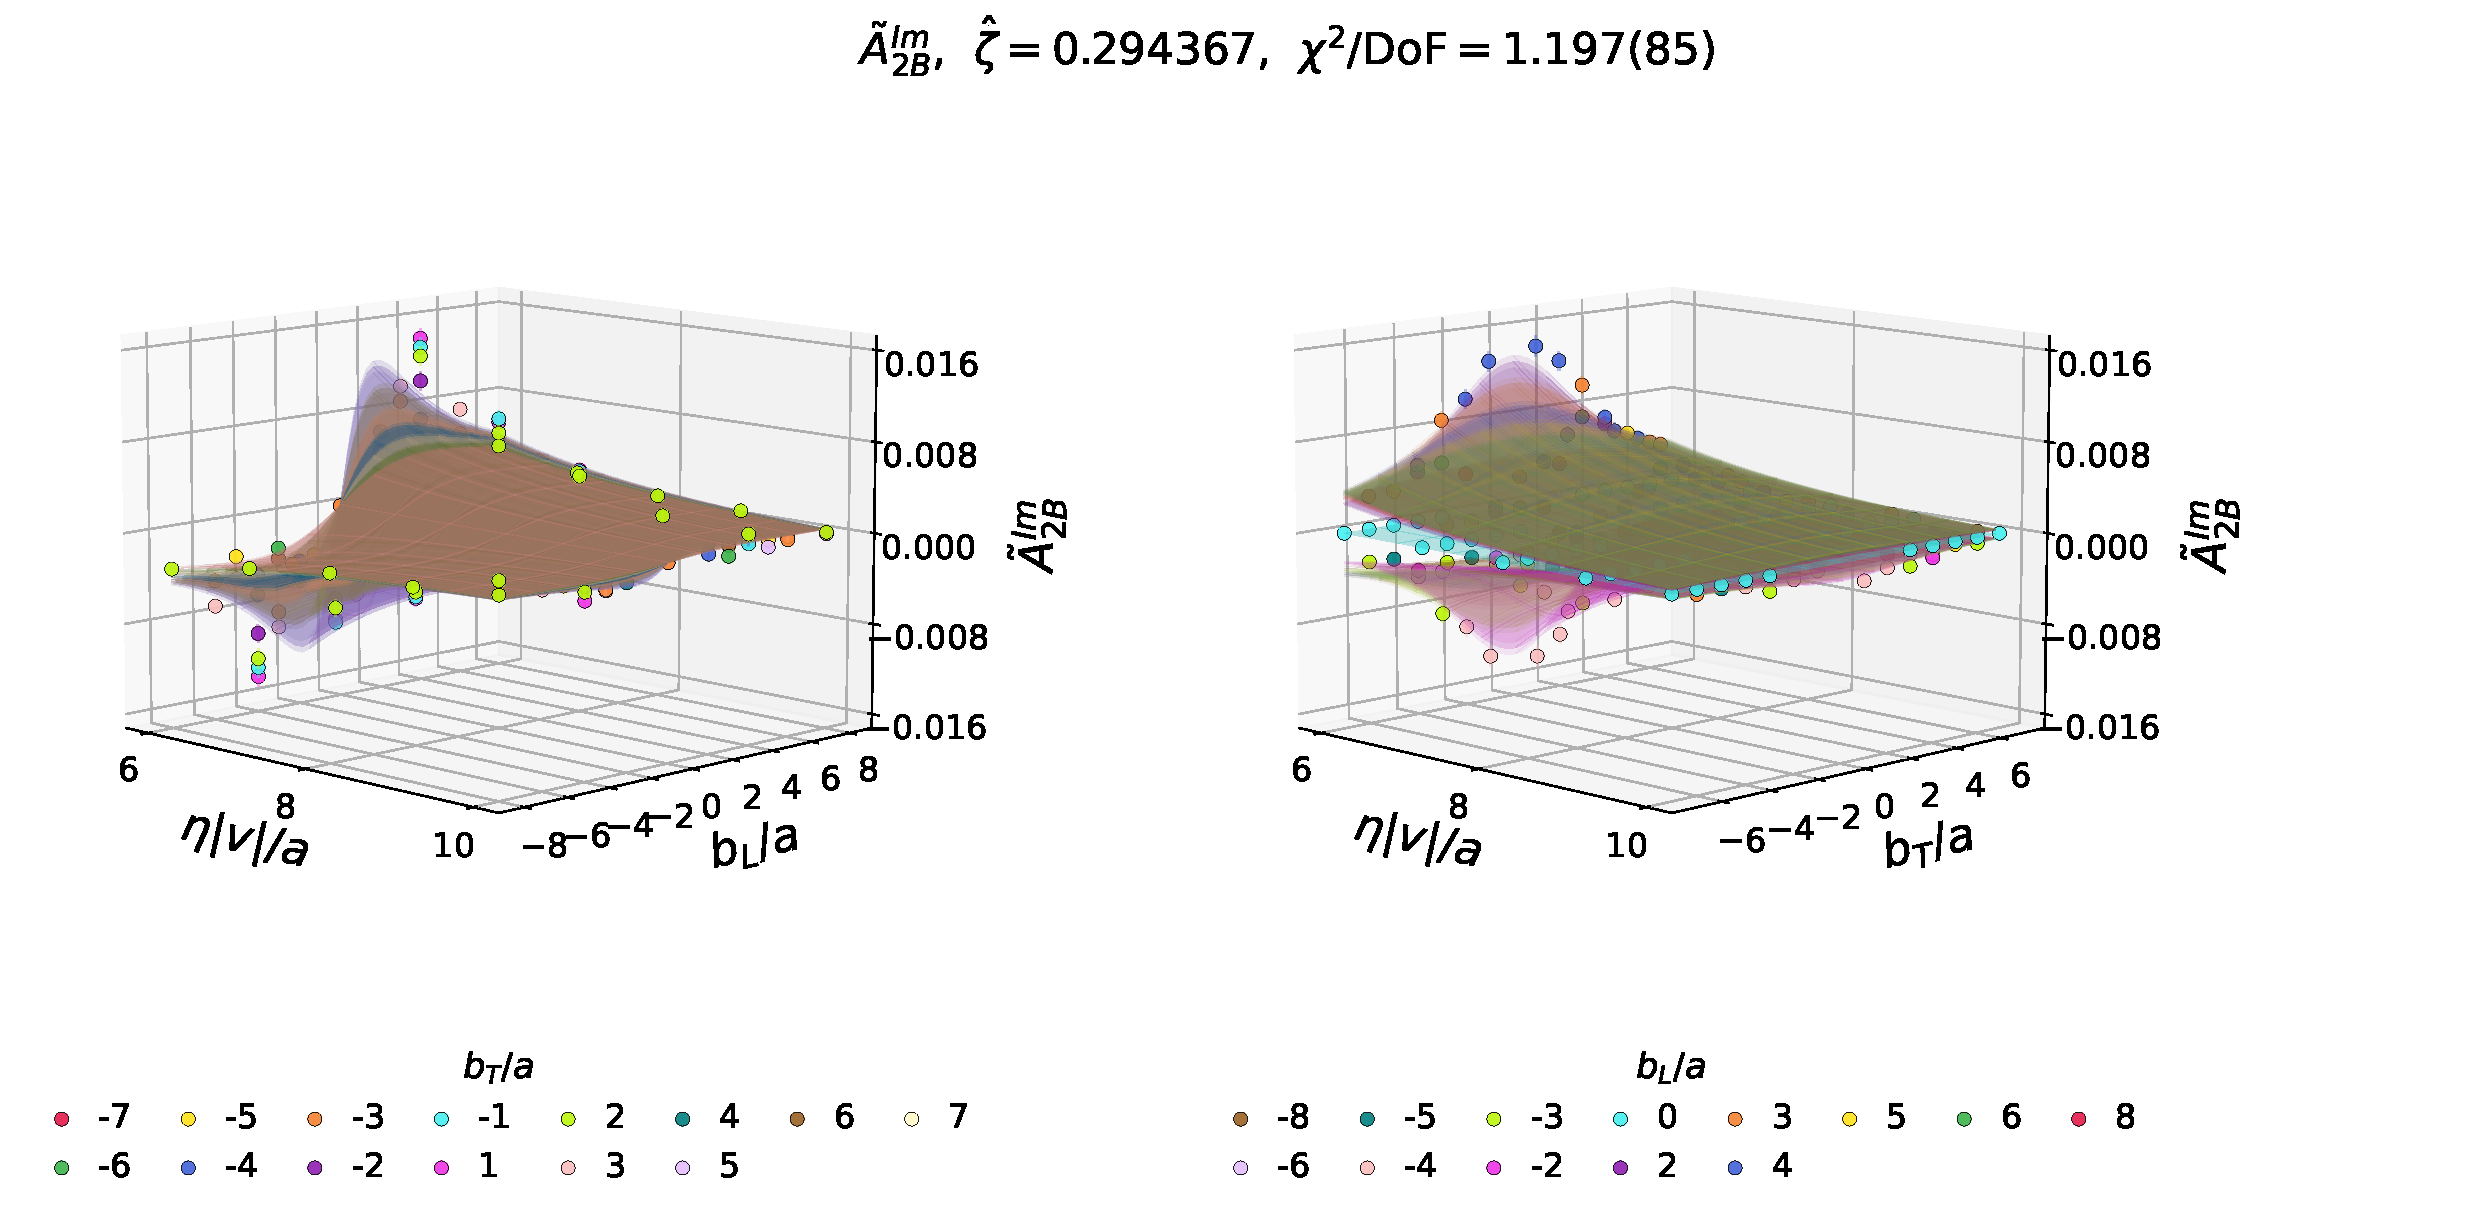
\includegraphics[width=\linewidth,height=.70\textheight,keepaspectratio]{fitting/ImA2B_PL-2_WithFit_3D.pdf}
\par\small Spatial coordinates: $(b_L,b_T,\eta)$. All panels and data overlays retained.

\figsrc{Thesis: plots; ImA2B\_PL-2\_WithFit\_3D}
\end{frame}

\begin{frame}{Global fit: $\tAmp_{2B}^{\mathrm{Im}}$, $P_L=-2$}
\centering
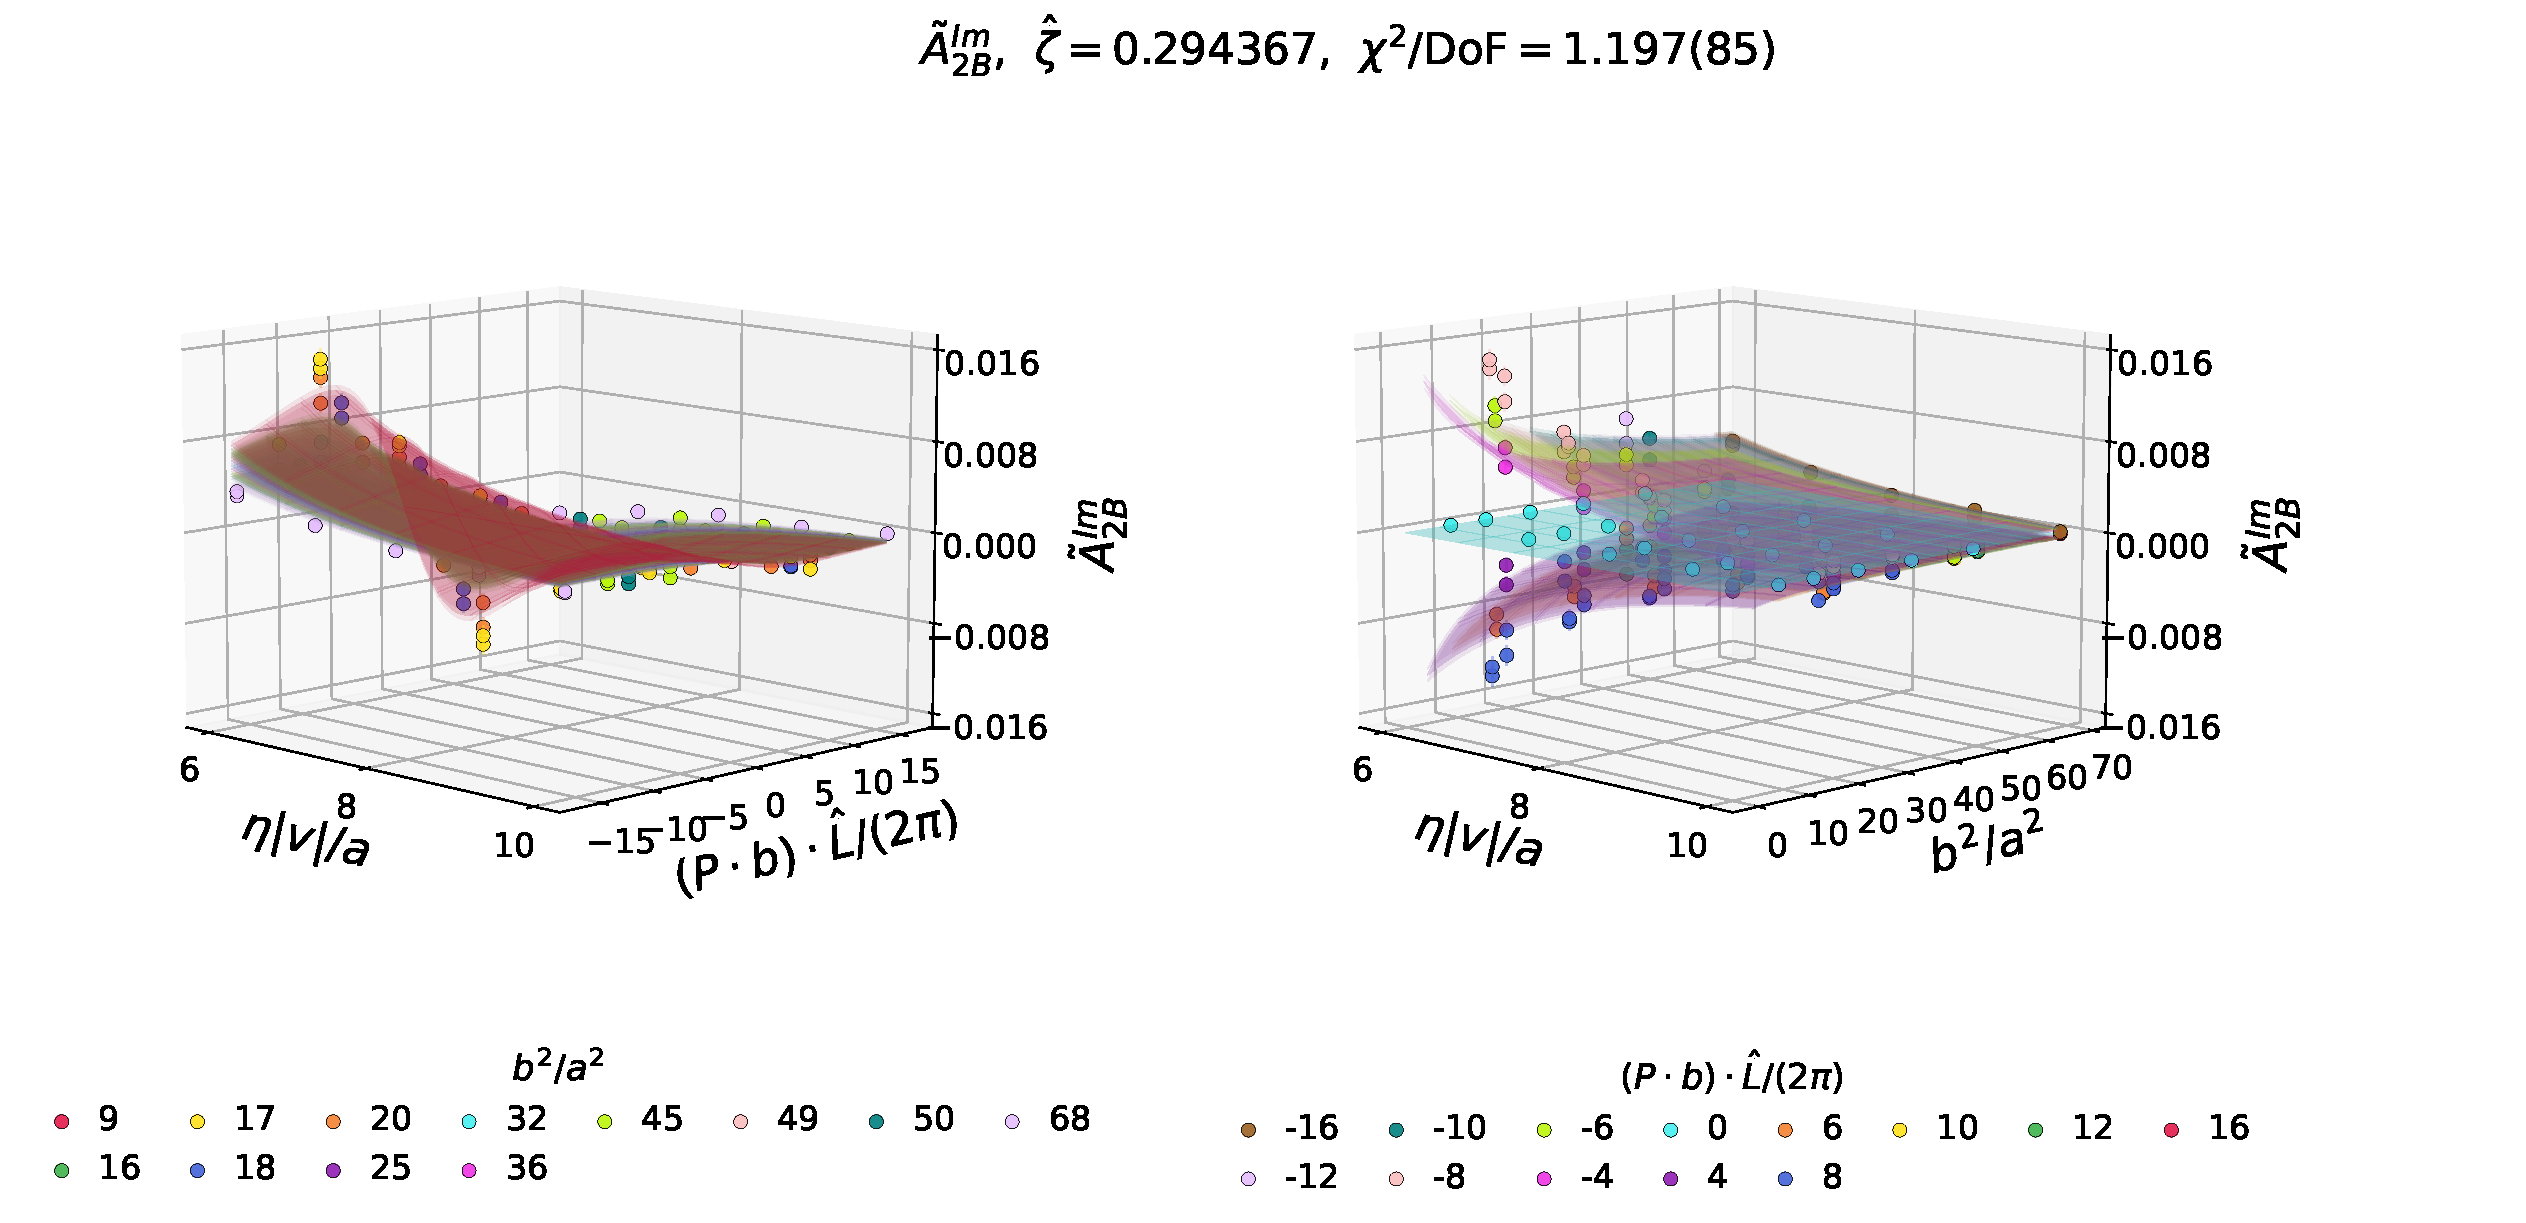
\includegraphics[width=\linewidth,height=.70\textheight,keepaspectratio]{fitting/ImA2B_Pb_bsq_PL-2_WithFit_3D.pdf}
\par\small Invariant coordinates: $(\nu,b^2,\eta)$. All panels and data overlays retained.

\figsrc{Thesis: plots; ImA2B\_Pb\_bsq\_PL-2\_WithFit\_3D}
\end{frame}

\begin{frame}{Fixed staple $\eta=8$: $\tAmp_{2B}^{\mathrm{Im}}$, $P_L=-2$}
\centering
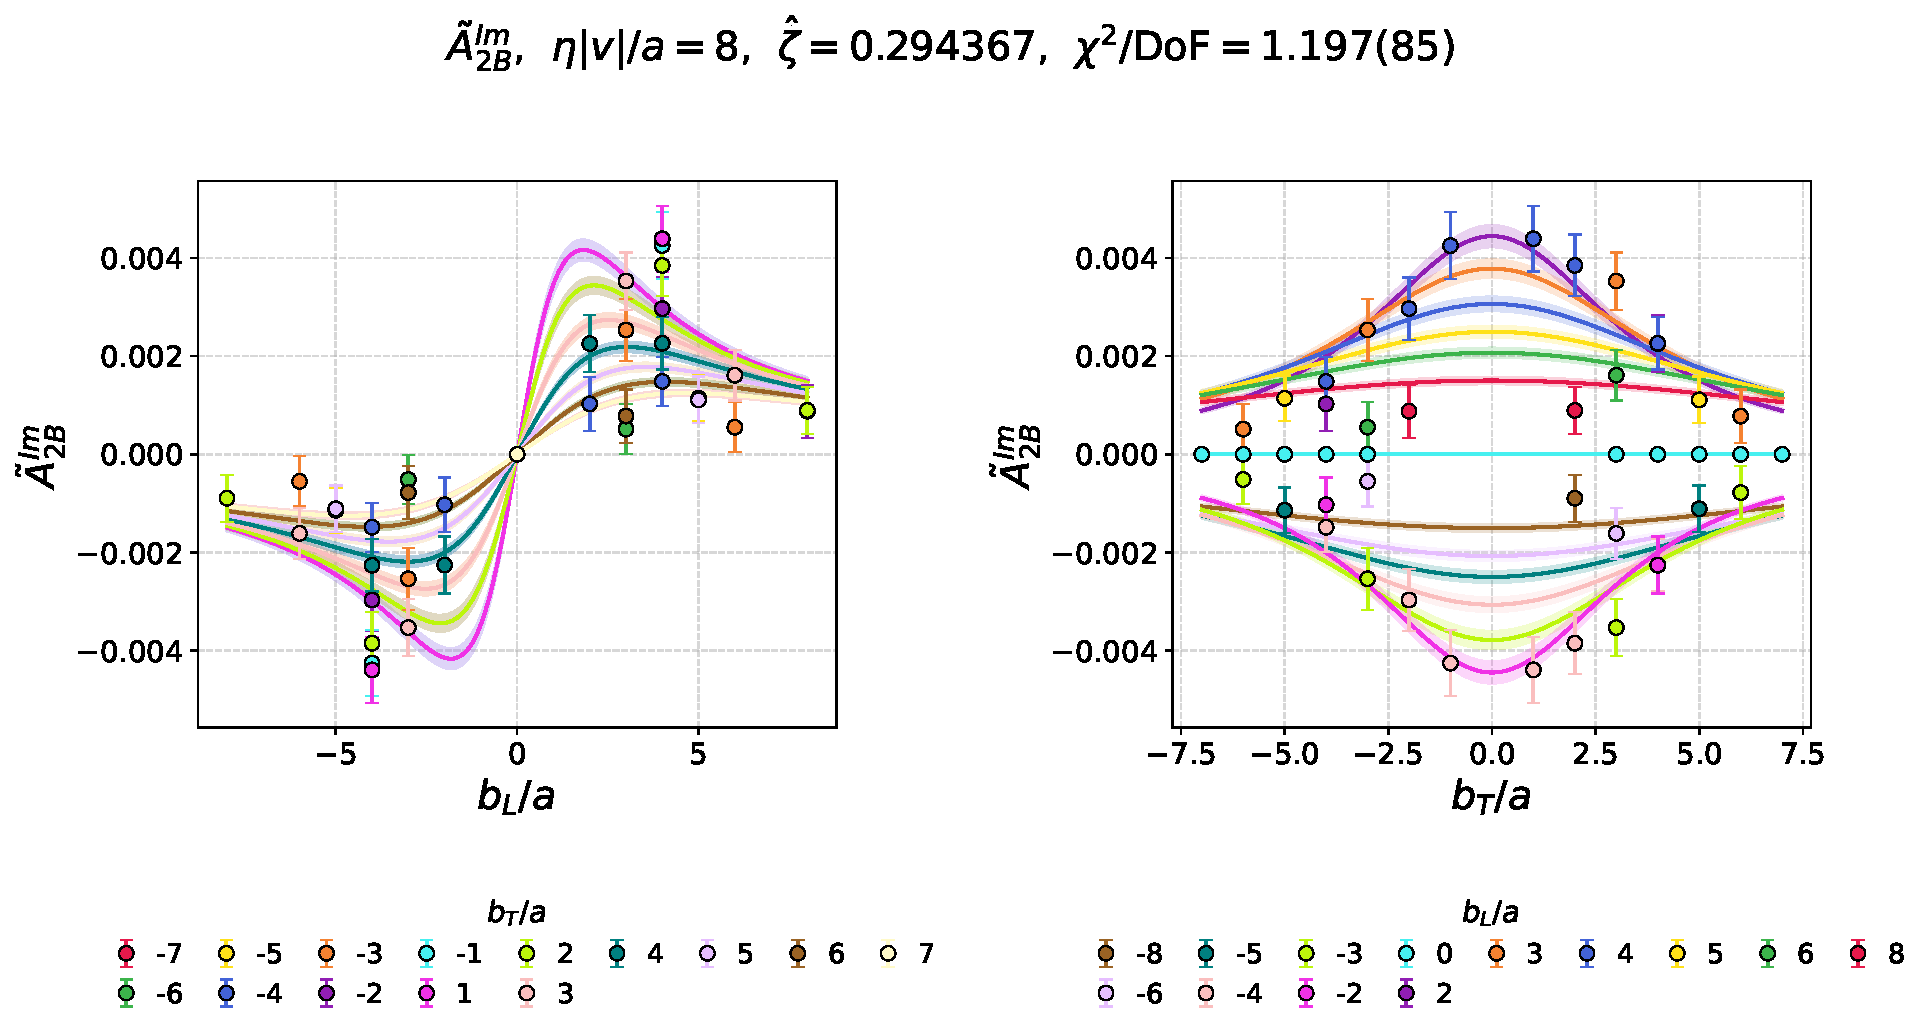
\includegraphics[width=\linewidth,height=.70\textheight,keepaspectratio]{fitting/ImA2B_eta8_PL-2_WithFit_2D.pdf}
\par\small Both spatial-coordinate slices. Same simultaneous fit, with Jackknife bands.

\figsrc{Thesis: plots; ImA2B\_eta8\_PL-2\_WithFit\_2D}
\end{frame}

\begin{frame}{Fixed staple $\eta=8$: $\tAmp_{2B}^{\mathrm{Im}}$, $P_L=-2$}
\centering
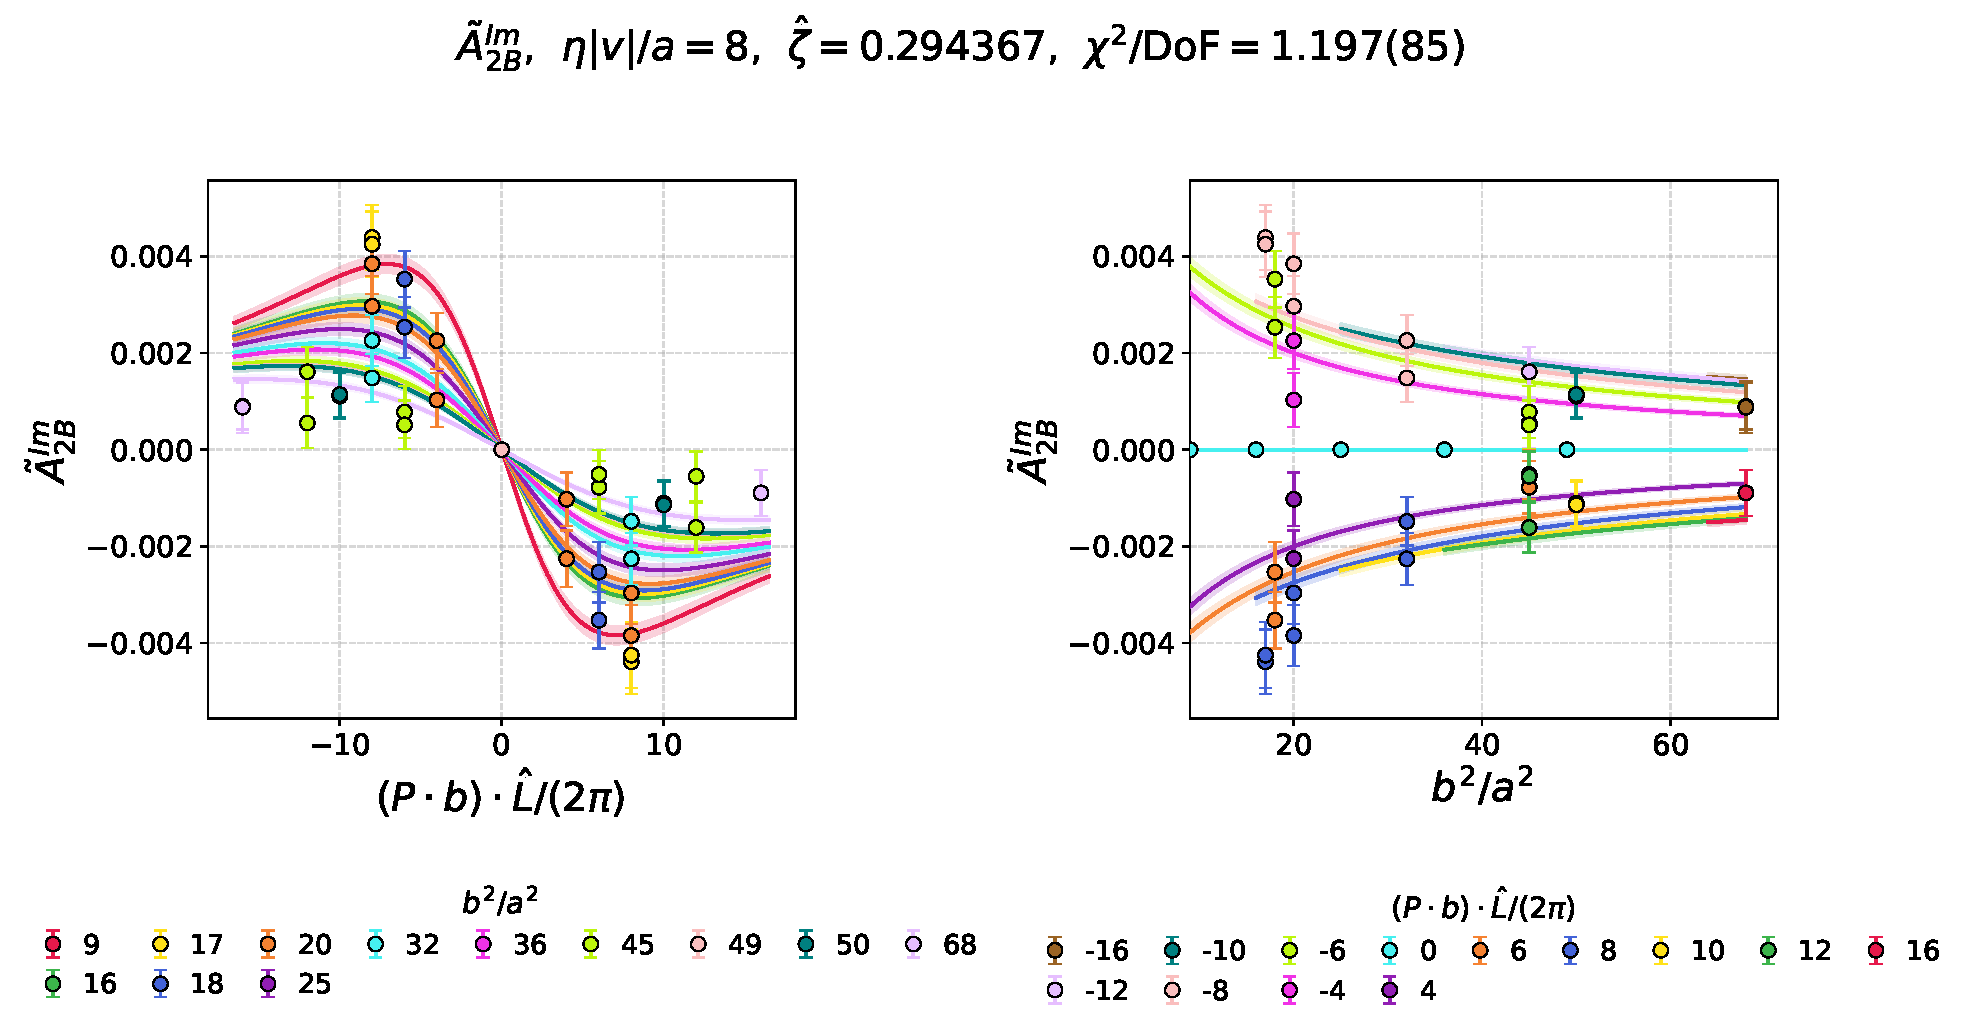
\includegraphics[width=\linewidth,height=.70\textheight,keepaspectratio]{fitting/ImA2B_Pb_bsq_eta8_PL-2_WithFit_2D.pdf}
\par\small Both invariant-coordinate slices. Same simultaneous fit, with Jackknife bands.

\figsrc{Thesis: plots; ImA2B\_Pb\_bsq\_eta8\_PL-2\_WithFit\_2D}
\end{frame}

\begin{frame}{Global fit: $\tAmp_{12B}^{\mathrm{Re}}$, $P_L=-2$}
\centering
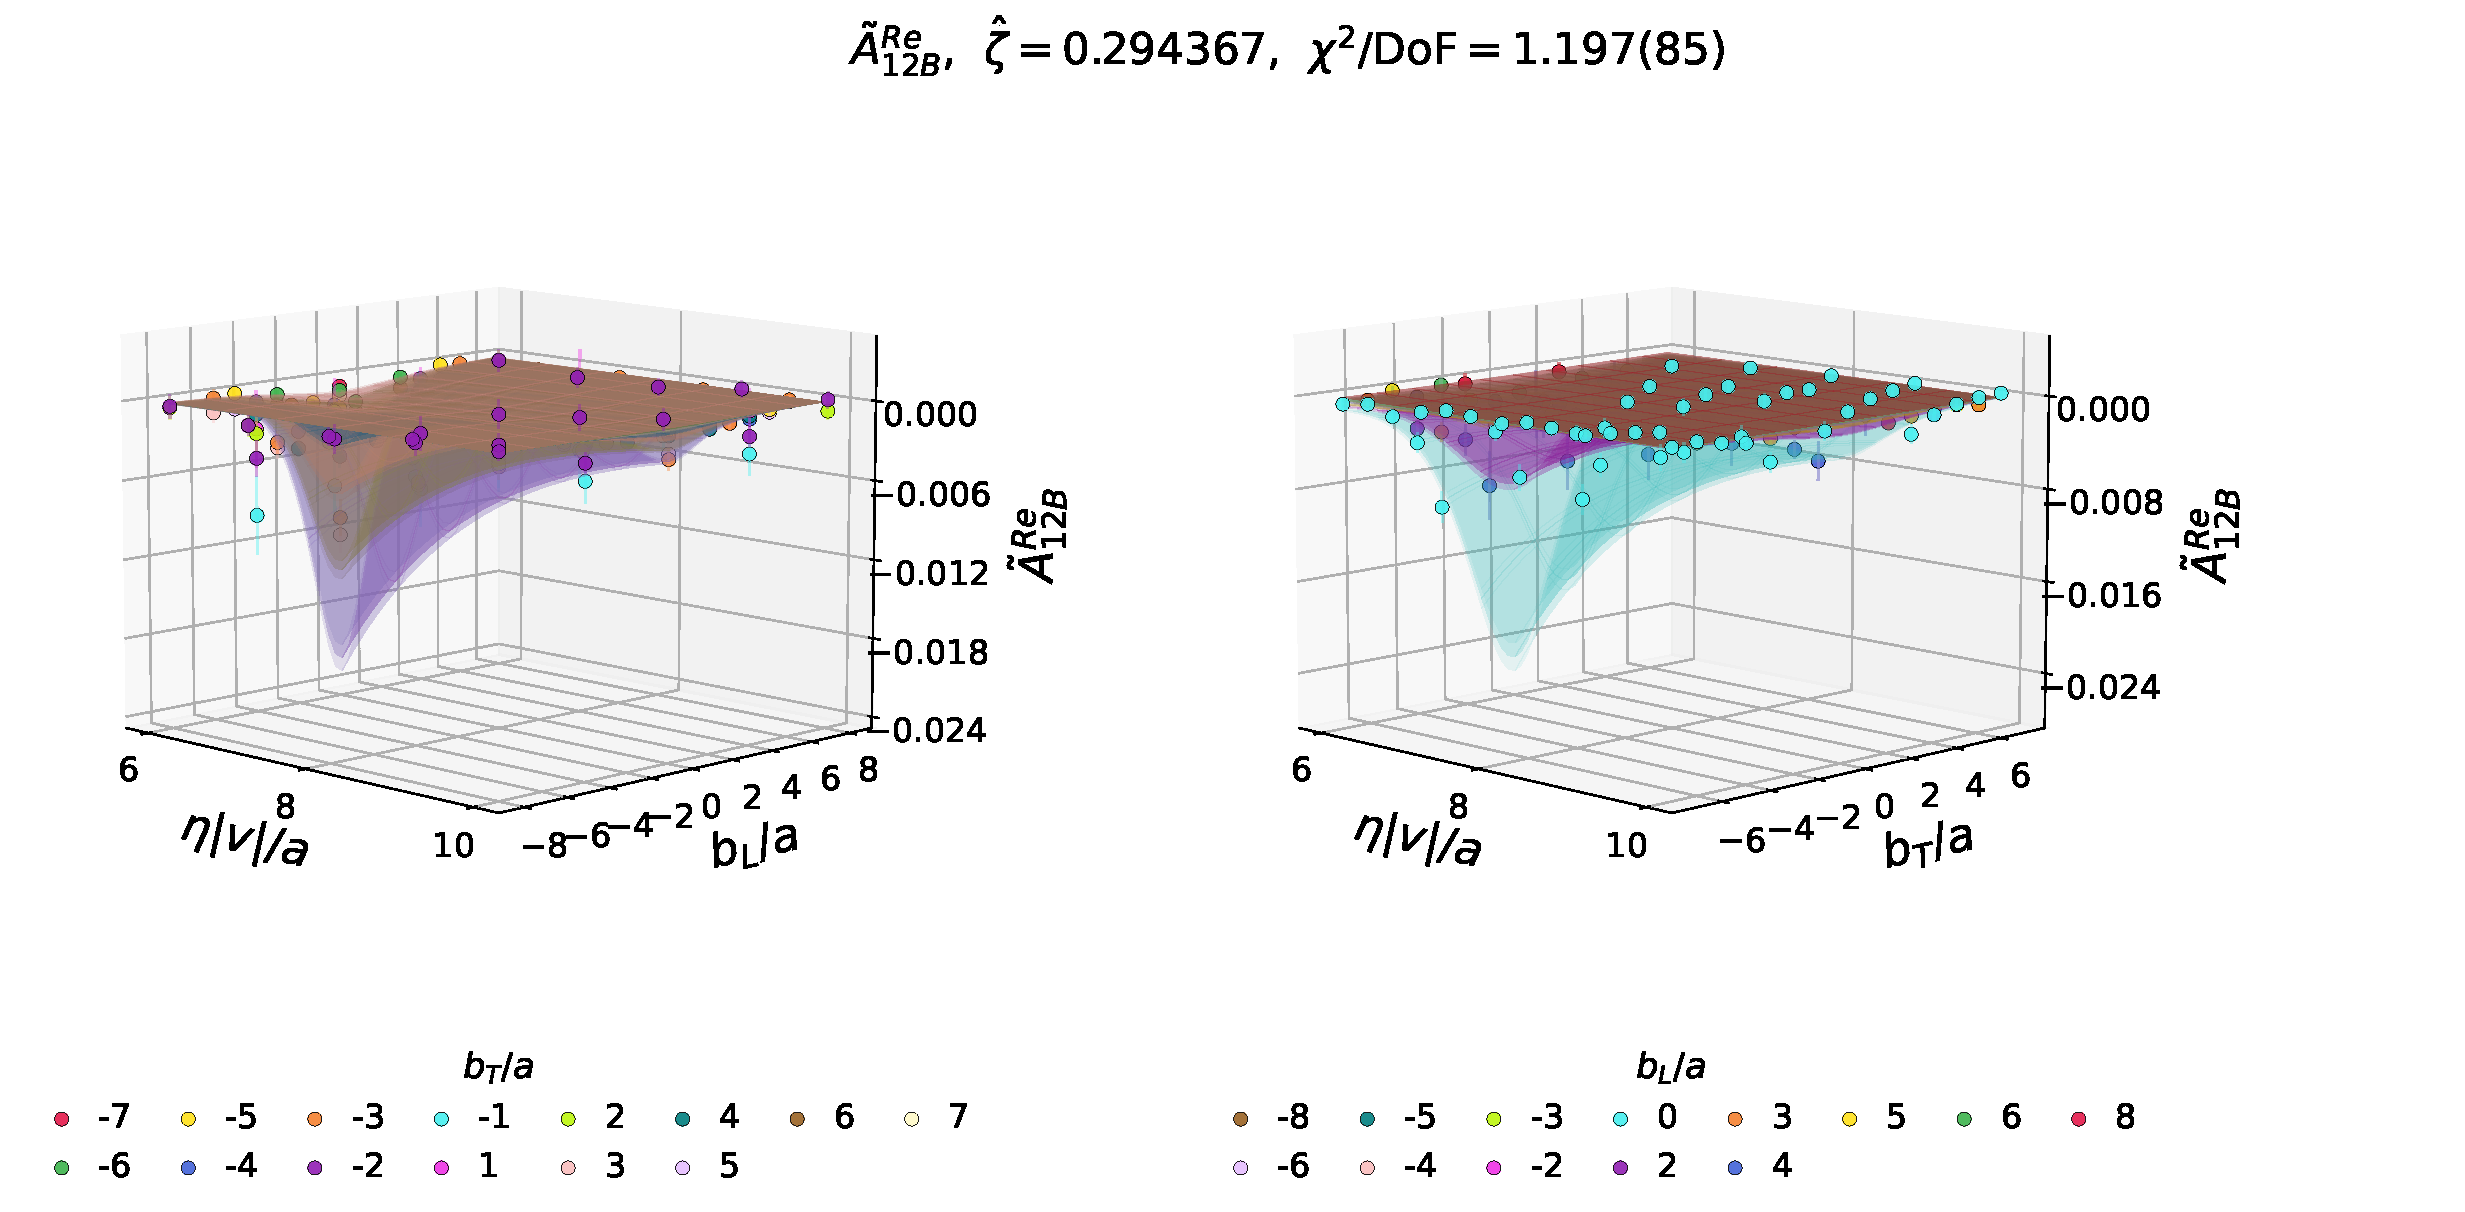
\includegraphics[width=\linewidth,height=.70\textheight,keepaspectratio]{fitting/ReA12B_PL-2_WithFit_3D.pdf}
\par\small Spatial coordinates: $(b_L,b_T,\eta)$. All panels and data overlays retained.

\figsrc{Thesis: plots; ReA12B\_PL-2\_WithFit\_3D}
\end{frame}

\begin{frame}{Global fit: $\tAmp_{12B}^{\mathrm{Re}}$, $P_L=-2$}
\centering
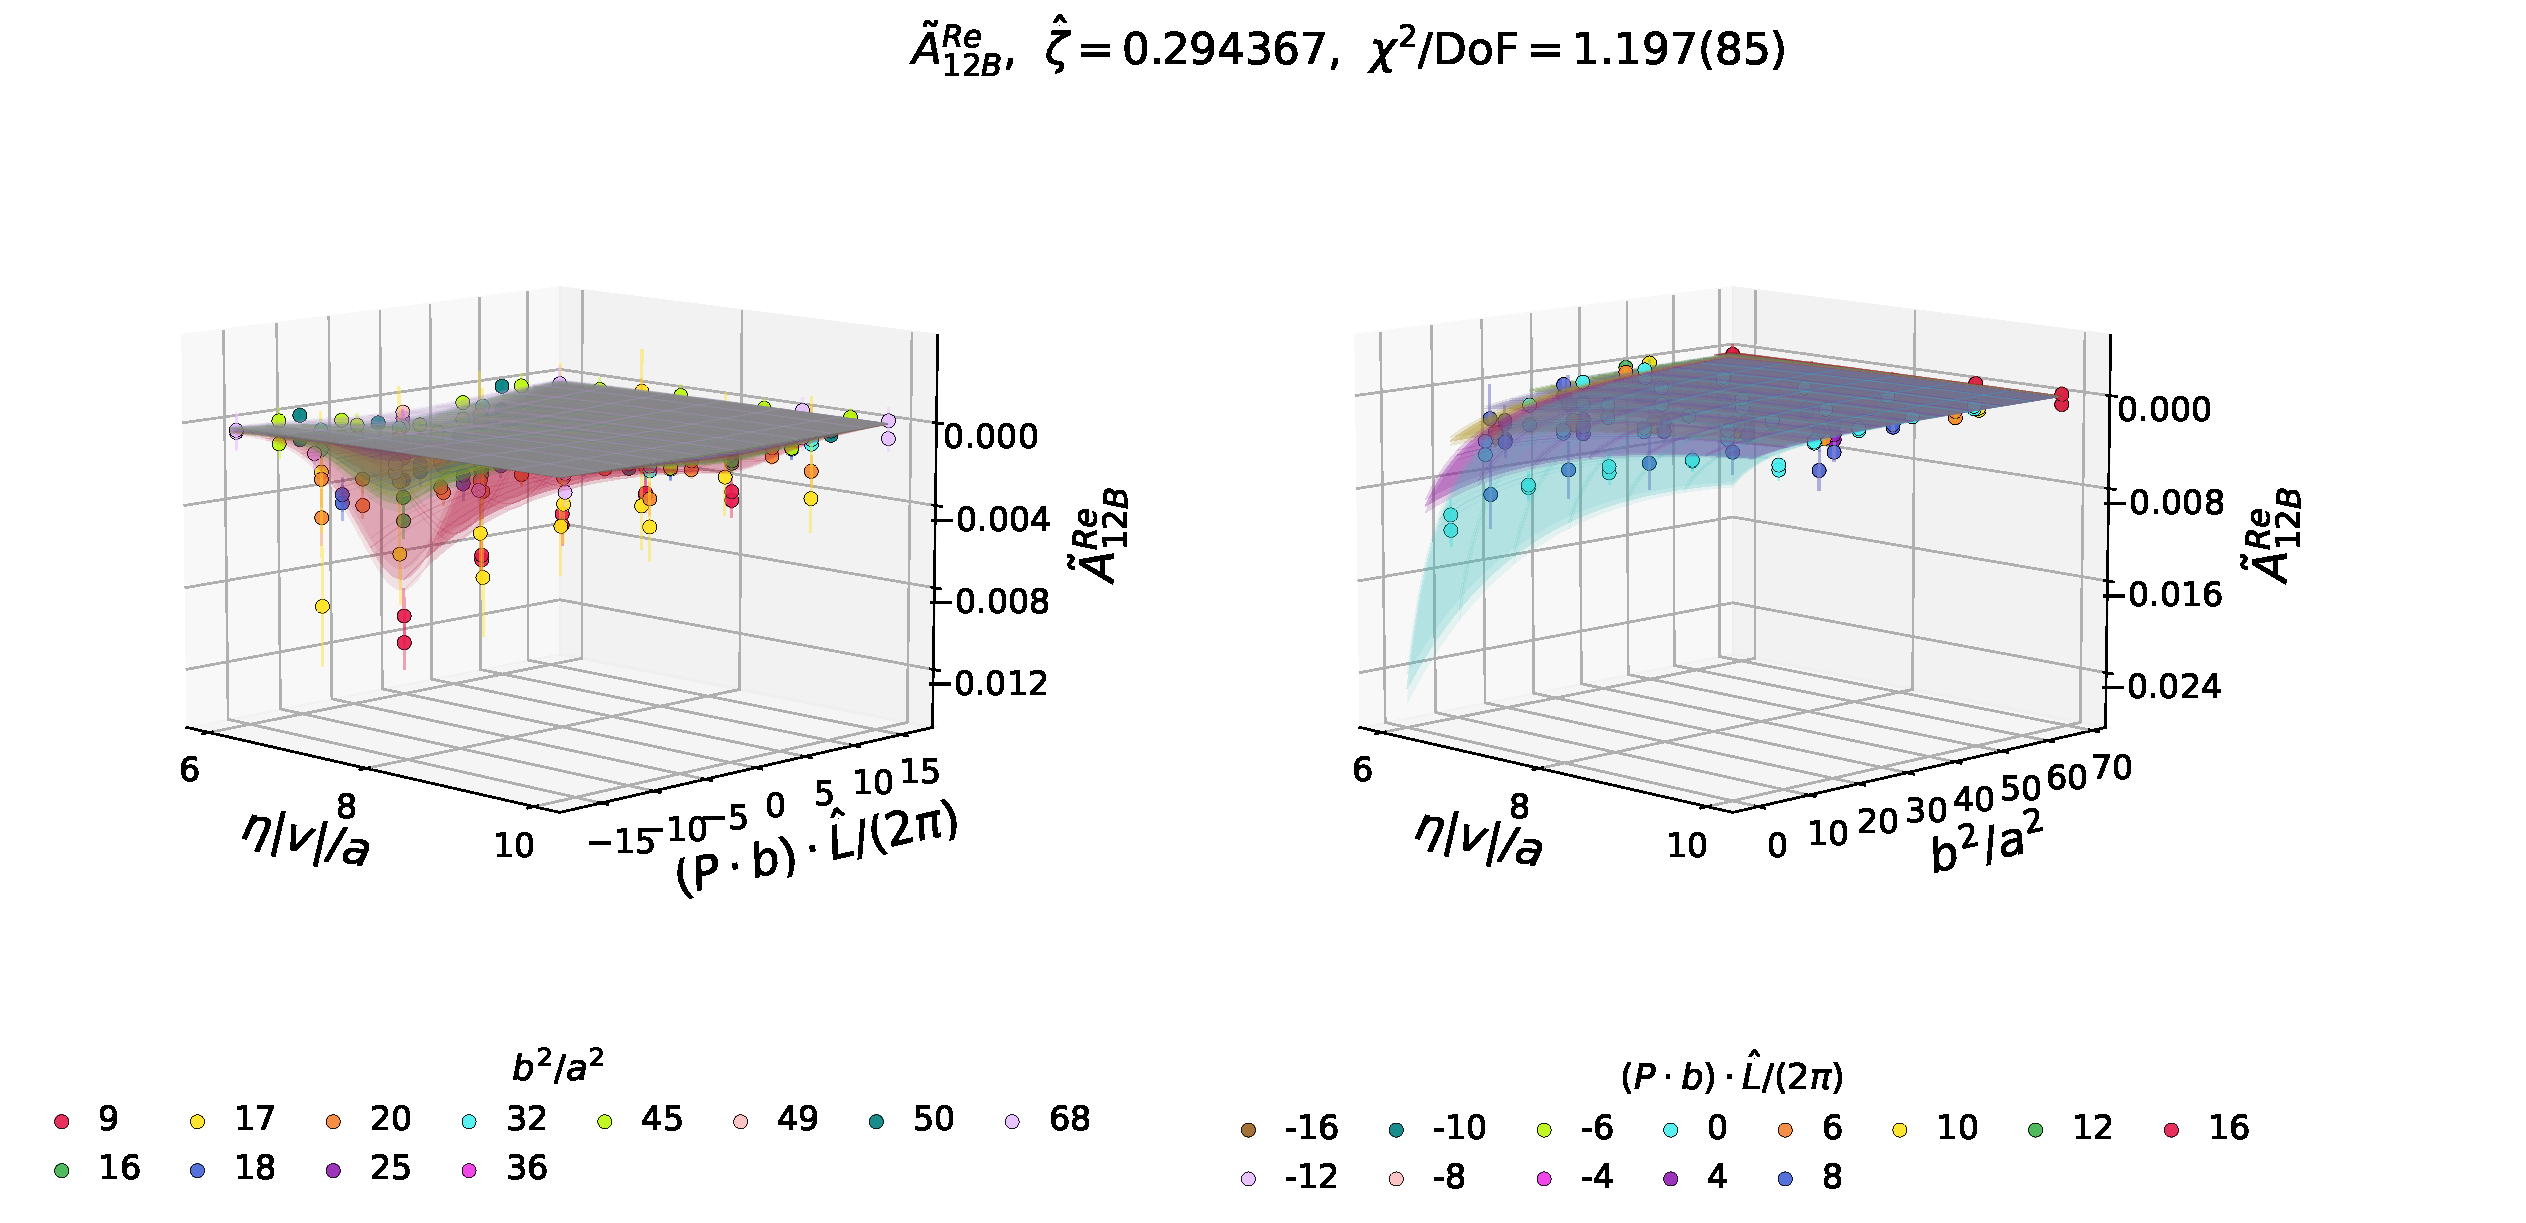
\includegraphics[width=\linewidth,height=.70\textheight,keepaspectratio]{fitting/ReA12B_Pb_bsq_PL-2_WithFit_3D.pdf}
\par\small Invariant coordinates: $(\nu,b^2,\eta)$. All panels and data overlays retained.

\figsrc{Thesis: plots; ReA12B\_Pb\_bsq\_PL-2\_WithFit\_3D}
\end{frame}

\begin{frame}{Fixed staple $\eta=8$: $\tAmp_{12B}^{\mathrm{Re}}$, $P_L=-2$}
\centering
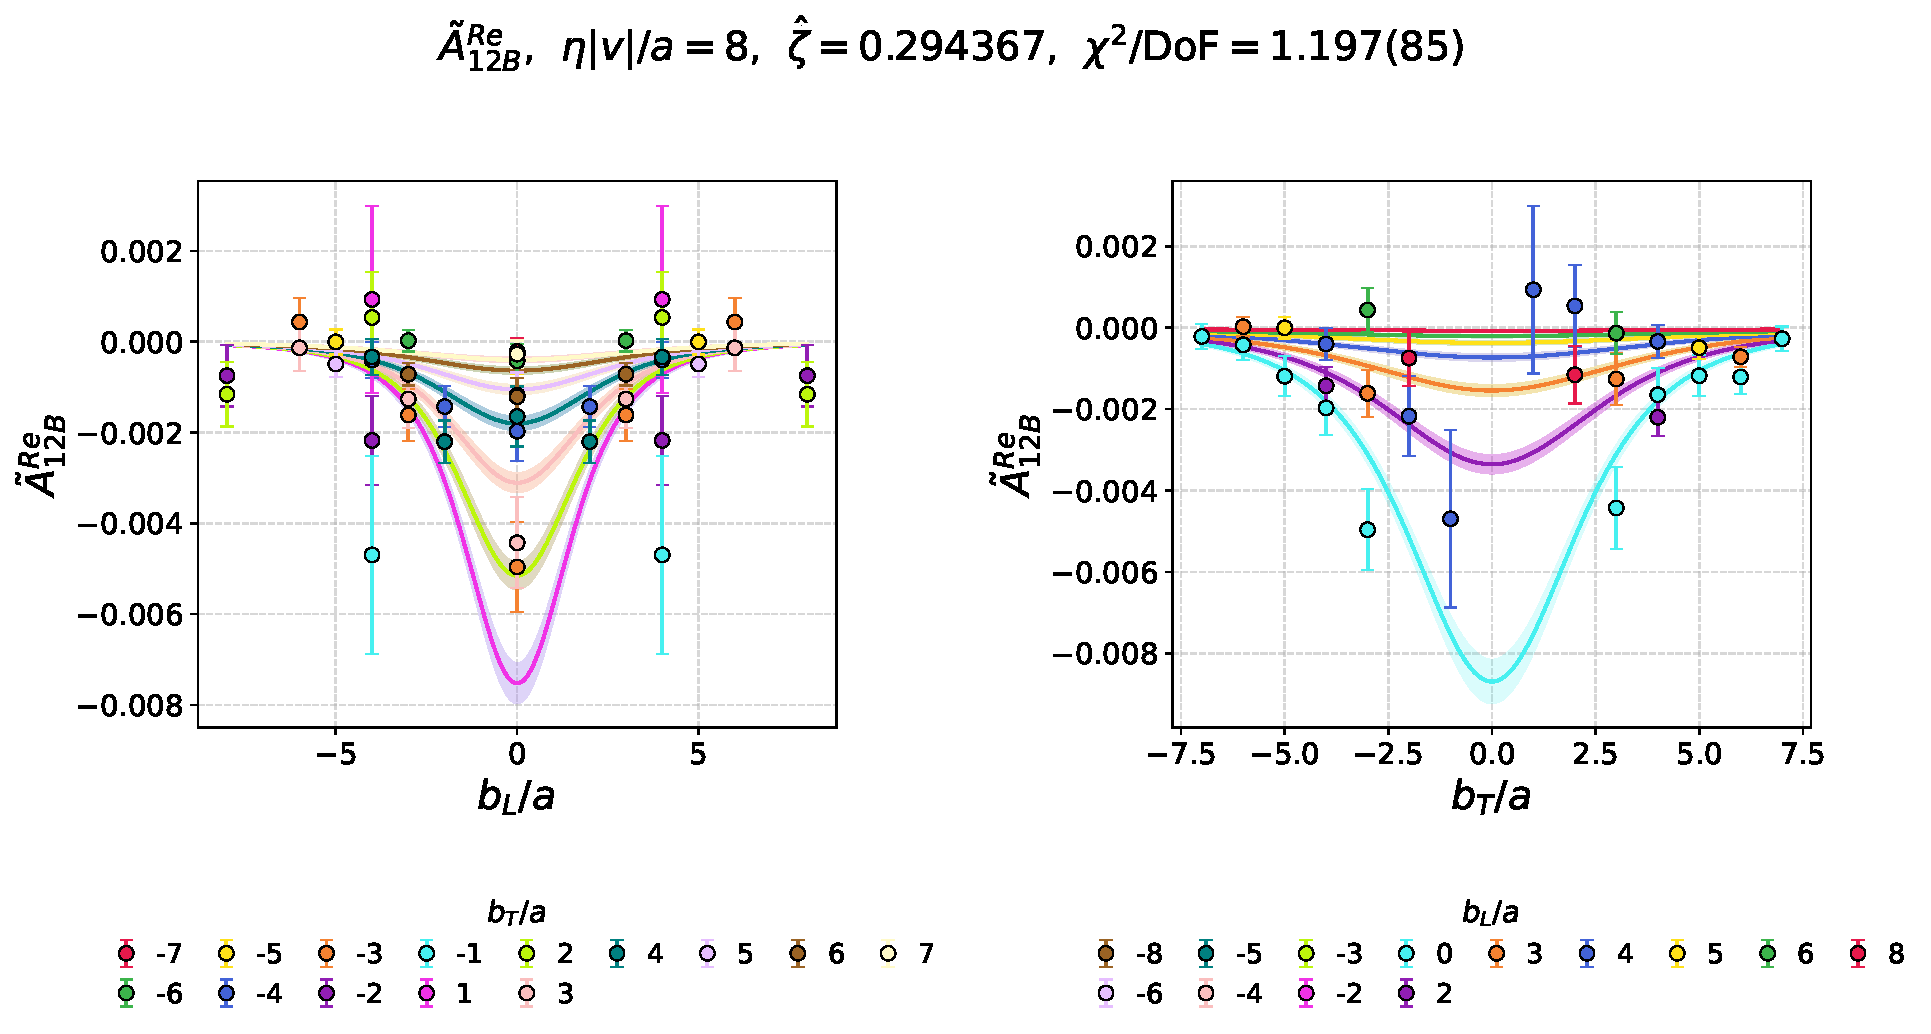
\includegraphics[width=\linewidth,height=.70\textheight,keepaspectratio]{fitting/ReA12B_eta8_PL-2_WithFit_2D.pdf}
\par\small Both spatial-coordinate slices. Same simultaneous fit, with Jackknife bands.

\figsrc{Thesis: plots; ReA12B\_eta8\_PL-2\_WithFit\_2D}
\end{frame}

\begin{frame}{Fixed staple $\eta=8$: $\tAmp_{12B}^{\mathrm{Re}}$, $P_L=-2$}
\centering
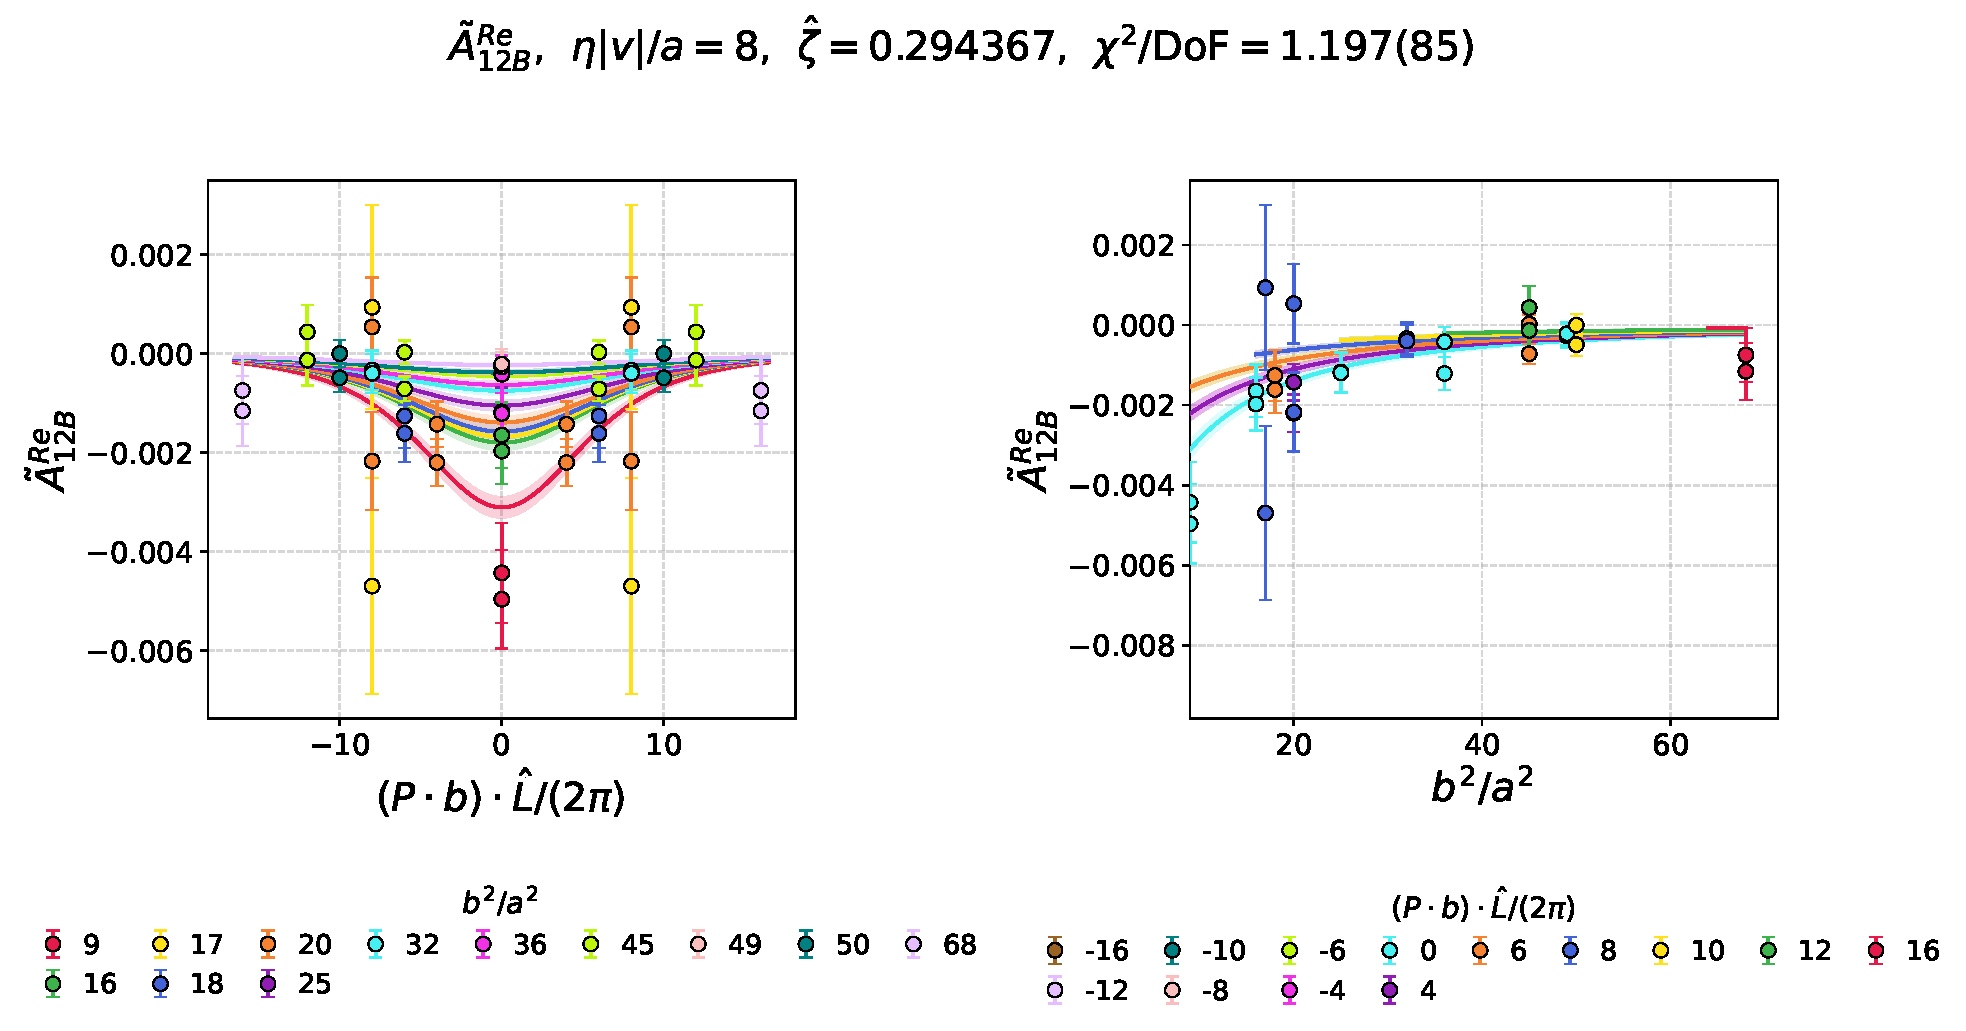
\includegraphics[width=\linewidth,height=.70\textheight,keepaspectratio]{fitting/ReA12B_Pb_bsq_eta8_PL-2_WithFit_2D.pdf}
\par\small Both invariant-coordinate slices. Same simultaneous fit, with Jackknife bands.

\figsrc{Thesis: plots; ReA12B\_Pb\_bsq\_eta8\_PL-2\_WithFit\_2D}
\end{frame}

\begin{frame}{Integrated Fourier results: $P_L=-2$}
\small\renewcommand{\arraystretch}{1.8}\begin{tabular}{lcccc}\toprule Integral & $(-\infty,\infty)$ & $[-1,1]$ & $[-1,0]$ & $[0,1]$\\\midrule
$\int dx\,E$ & 1.041(41) & 1.035(43) & 0.518(22) & 0.518(22) \\
$\int dx\,O$ & -6(176)e-17 & 7(444)e-17 & 0.257(13) & -0.257(13) \\
$\int dx\,\tilde f_1^{(0)}$ & 2.081(82) & 2.070(86) & 0.520(34) & 1.550(63) \\
$\int dx\,\tilde f_{1T}^{\perp(1)}$ & 0.451(27) & 0.451(27) & 0.225(14) & 0.225(14) \\
$m_N\int dx\,\tilde f_{1T}^{\perp(1)}/\int dx\,\tilde f_1^{(0)}$ & 0.233(14) & 0.234(14) & 0.466(36) & 0.1565(95) \\
\bottomrule\end{tabular}\par\medskip $b^2=9a^2$; all values and Jackknife uncertainties retained. Numerical values retain the source normalization. The last row is in GeV.
\figsrc{Thesis: SimultaneousFitsCov/Integration\_Table\_PL-2\_bmin3\_b2-9.tex}
\end{frame}

\begin{frame}{Fourier results (2D): $P_L=-2$, unpolarized}
\centering
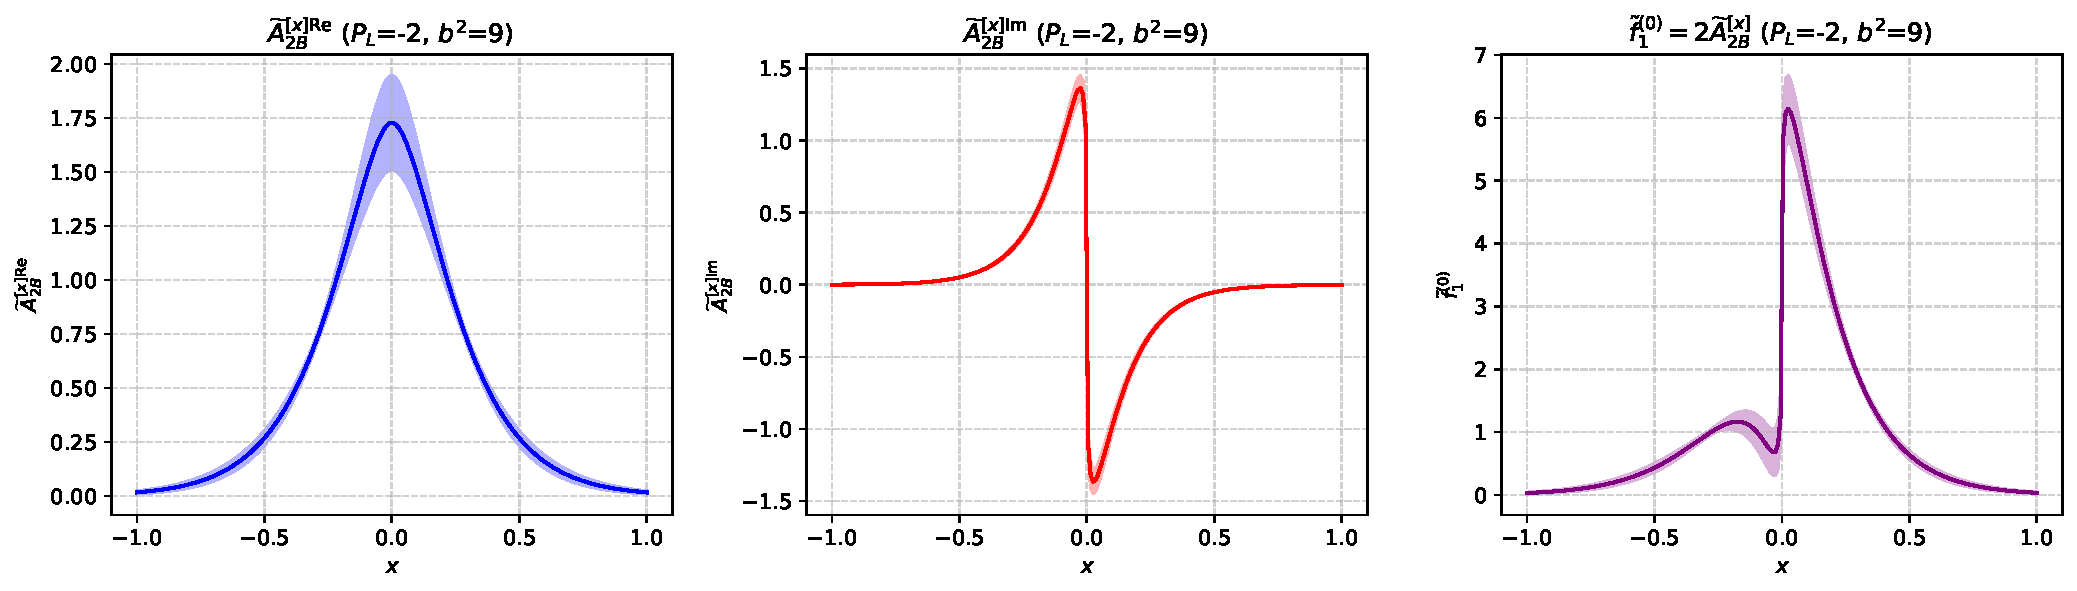
\includegraphics[width=\linewidth,height=.70\textheight,keepaspectratio]{fitting/FT_xdep_A2B_A12B_bmin3_eta610_b2-9_PL-2__row1.pdf}
\par\small Even, odd, and unpolarized transforms. Fixed $b^2=9a^2$.

\figsrc{Thesis: SimultaneousFitsCov; FT\_xdep\_A2B\_A12B\_bmin3\_eta610\_b2-9\_PL-2}
\end{frame}

\begin{frame}{Fourier results (2D): $P_L=-2$, Sivers}
\centering
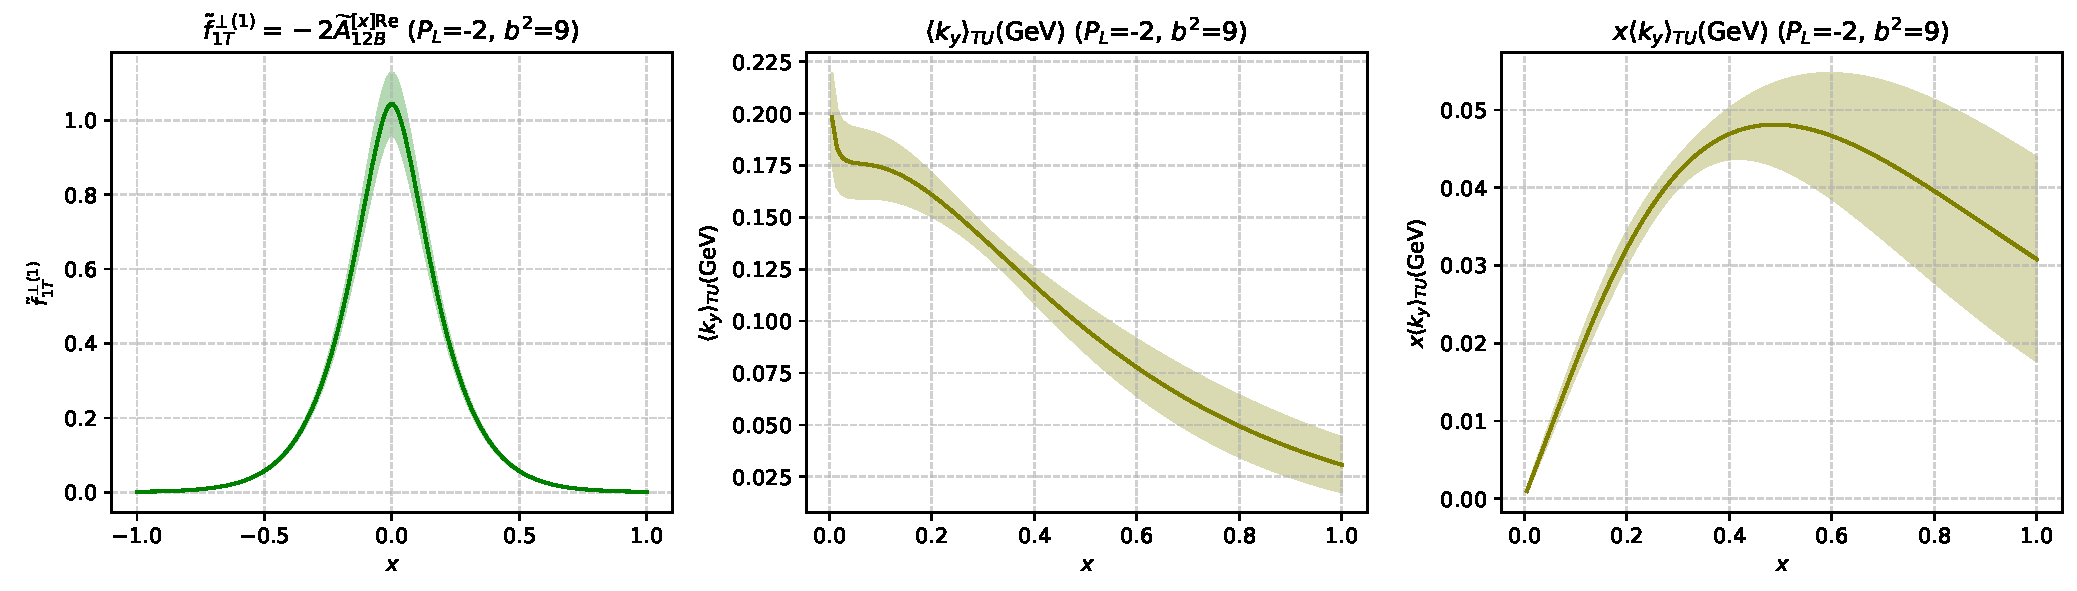
\includegraphics[width=\linewidth,height=.70\textheight,keepaspectratio]{fitting/FT_xdep_A2B_A12B_bmin3_eta610_b2-9_PL-2__row2.pdf}
\par\small Sivers transform, shift, and $x\langle k_y\rangle_{TU}$. Fixed $b^2=9a^2$.

\figsrc{Thesis: SimultaneousFitsCov; FT\_xdep\_A2B\_A12B\_bmin3\_eta610\_b2-9\_PL-2}
\end{frame}

\begin{frame}{Fourier results (3D): $P_L=-2$, unpolarized}
\centering
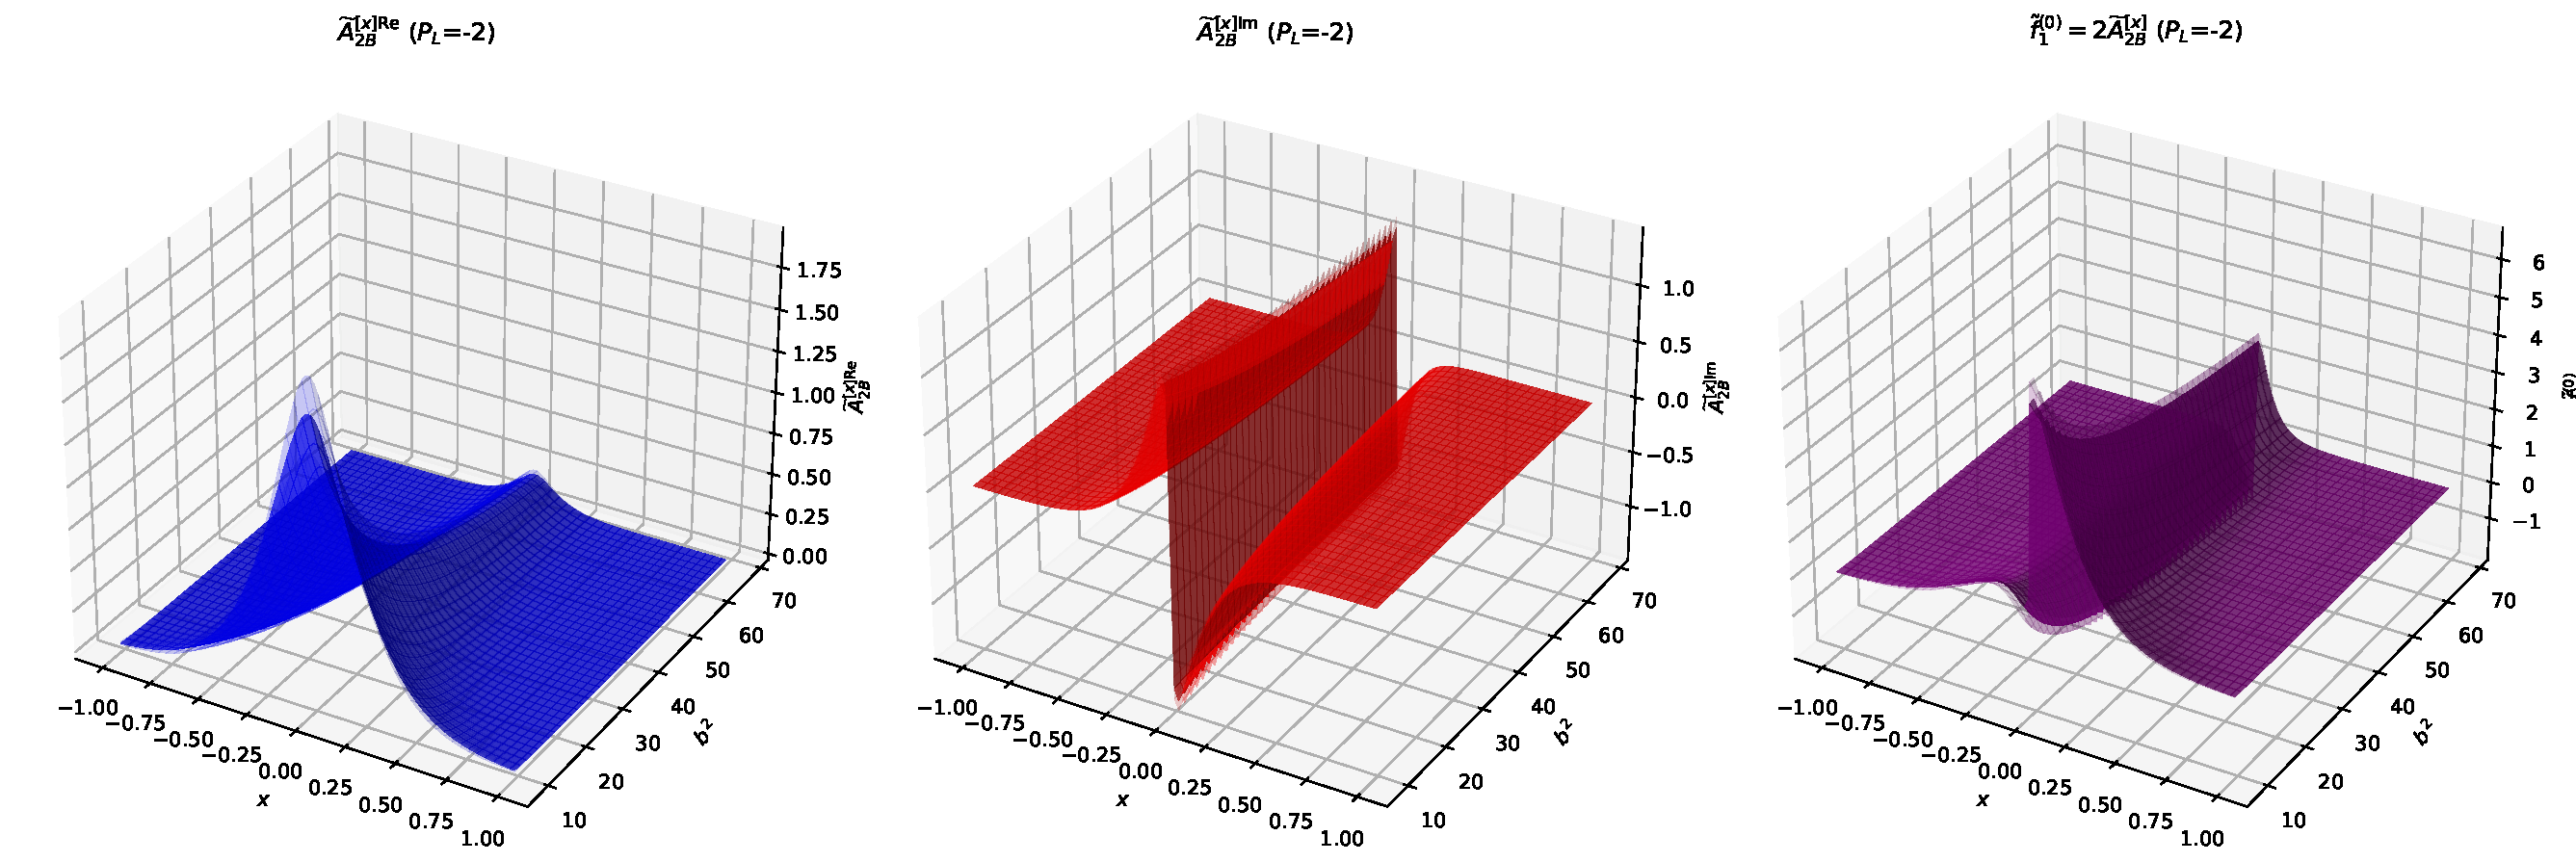
\includegraphics[width=\linewidth,height=.70\textheight,keepaspectratio]{fitting/FT_xdep_3D_A2B_A12B_bmin3_eta610_PL-2__row1.pdf}
\par\small Even, odd, and unpolarized transforms. Full $b^2/a^2\in[9,68]$ dependence.

\figsrc{Thesis: SimultaneousFitsCov; FT\_xdep\_3D\_A2B\_A12B\_bmin3\_eta610\_PL-2}
\end{frame}

\begin{frame}{Fourier results (3D): $P_L=-2$, Sivers}
\centering
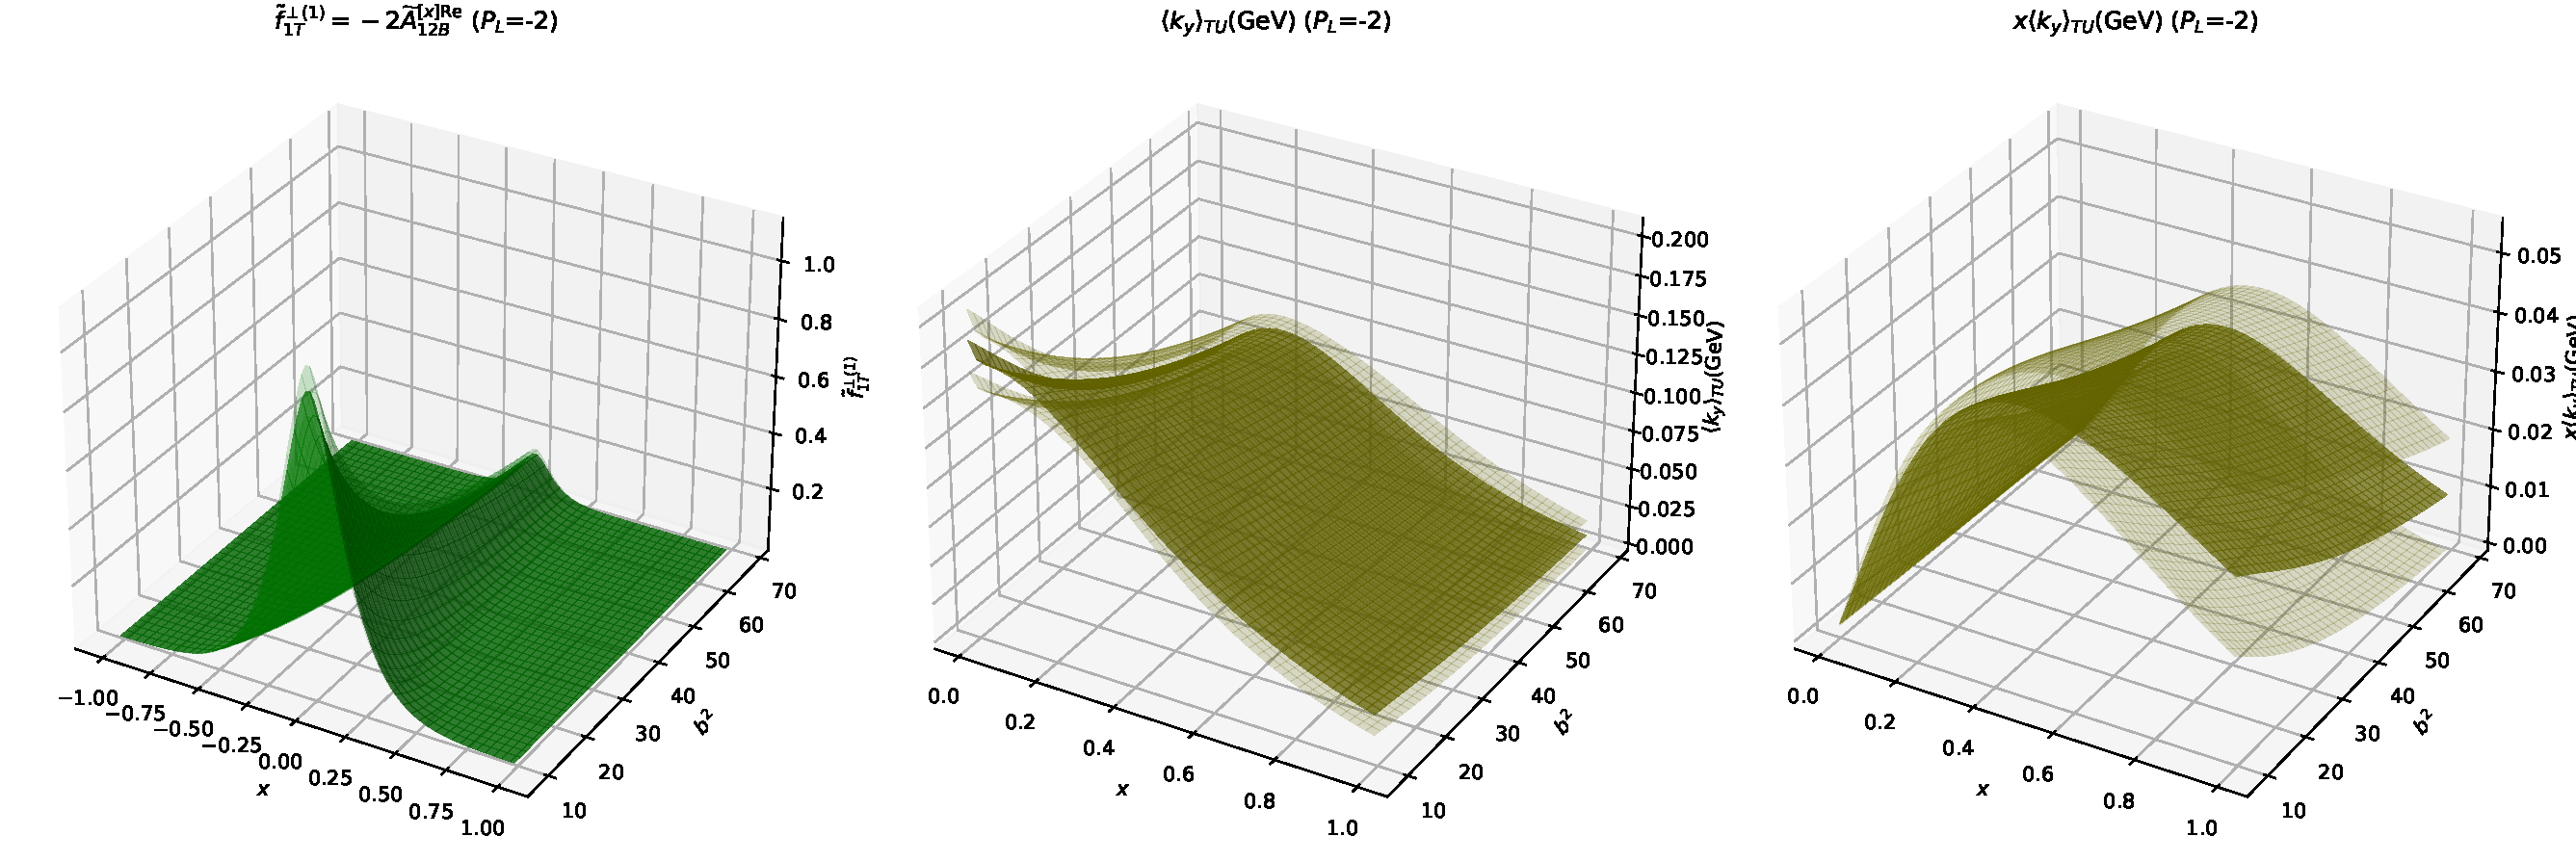
\includegraphics[width=\linewidth,height=.70\textheight,keepaspectratio]{fitting/FT_xdep_3D_A2B_A12B_bmin3_eta610_PL-2__row2.pdf}
\par\small Sivers transform, shift, and $x\langle k_y\rangle_{TU}$. Full $b^2/a^2\in[9,68]$ dependence.

\figsrc{Thesis: SimultaneousFitsCov; FT\_xdep\_3D\_A2B\_A12B\_bmin3\_eta610\_PL-2}
\end{frame}

\begin{frame}{Simultaneous fit parameters: $P_L=-3$}
\small $|\vect b|\ge3a$, $6\le\eta\le10$; reported $\chi^2_{\rm aug}/N_{\rm data}=0.712(66)$.\par\medskip
\begin{columns}[t]\begin{column}{.32\textwidth}\centering $\tAmp_{2B}^{\mathrm{Re}}$\par\medskip\renewcommand{\arraystretch}{1.3}\begin{tabular}{cc}\toprule Parameter & Value\\\midrule
$a$ & $4.0061(31)$ \\
$c$ & $0.45(12)$ \\
$d$ & $0.136(11)$ \\
$k_1$ & $12.284(11)$ \\
$k_2$ & $-36.1973(19)$ \\
$j$ & $2.085(10)$ \\
$f$ & $0.540(15)$ \\\bottomrule\end{tabular}\end{column}\begin{column}{.32\textwidth}\centering $\tAmp_{2B}^{\mathrm{Im}}$\par\medskip\renewcommand{\arraystretch}{1.3}\begin{tabular}{cc}\toprule Parameter & Value\\\midrule
$a''$ & $0.328(11)$ \\
$c''$ & $0.163(15)$ \\
$d''$ & $0.147(13)$ \\
$j''$ & $1.057(15)$ \\
$f$ & $0.540(15)$ \\\bottomrule\end{tabular}\end{column}\begin{column}{.32\textwidth}\centering $\tAmp_{12B}^{\mathrm{Re}}$\par\medskip\renewcommand{\arraystretch}{1.3}\begin{tabular}{cc}\toprule Parameter & Value\\\midrule
$a'$ & $0.569(13)$ \\
$c'$ & $0.100(17)$ \\
$d'$ & $0.094(16)$ \\
$j'$ & $1.9969(49)$ \\
$f$ & $0.540(15)$ \\\bottomrule\end{tabular}\end{column}\end{columns}
\figsrc{Thesis: SimultaneousFitsCov/Fit\_Table\_PL-3\_bmin3.tex}
\end{frame}

\begin{frame}{Global fit: $\tAmp_{2B}^{\mathrm{Re}}$, $P_L=-3$}
\centering
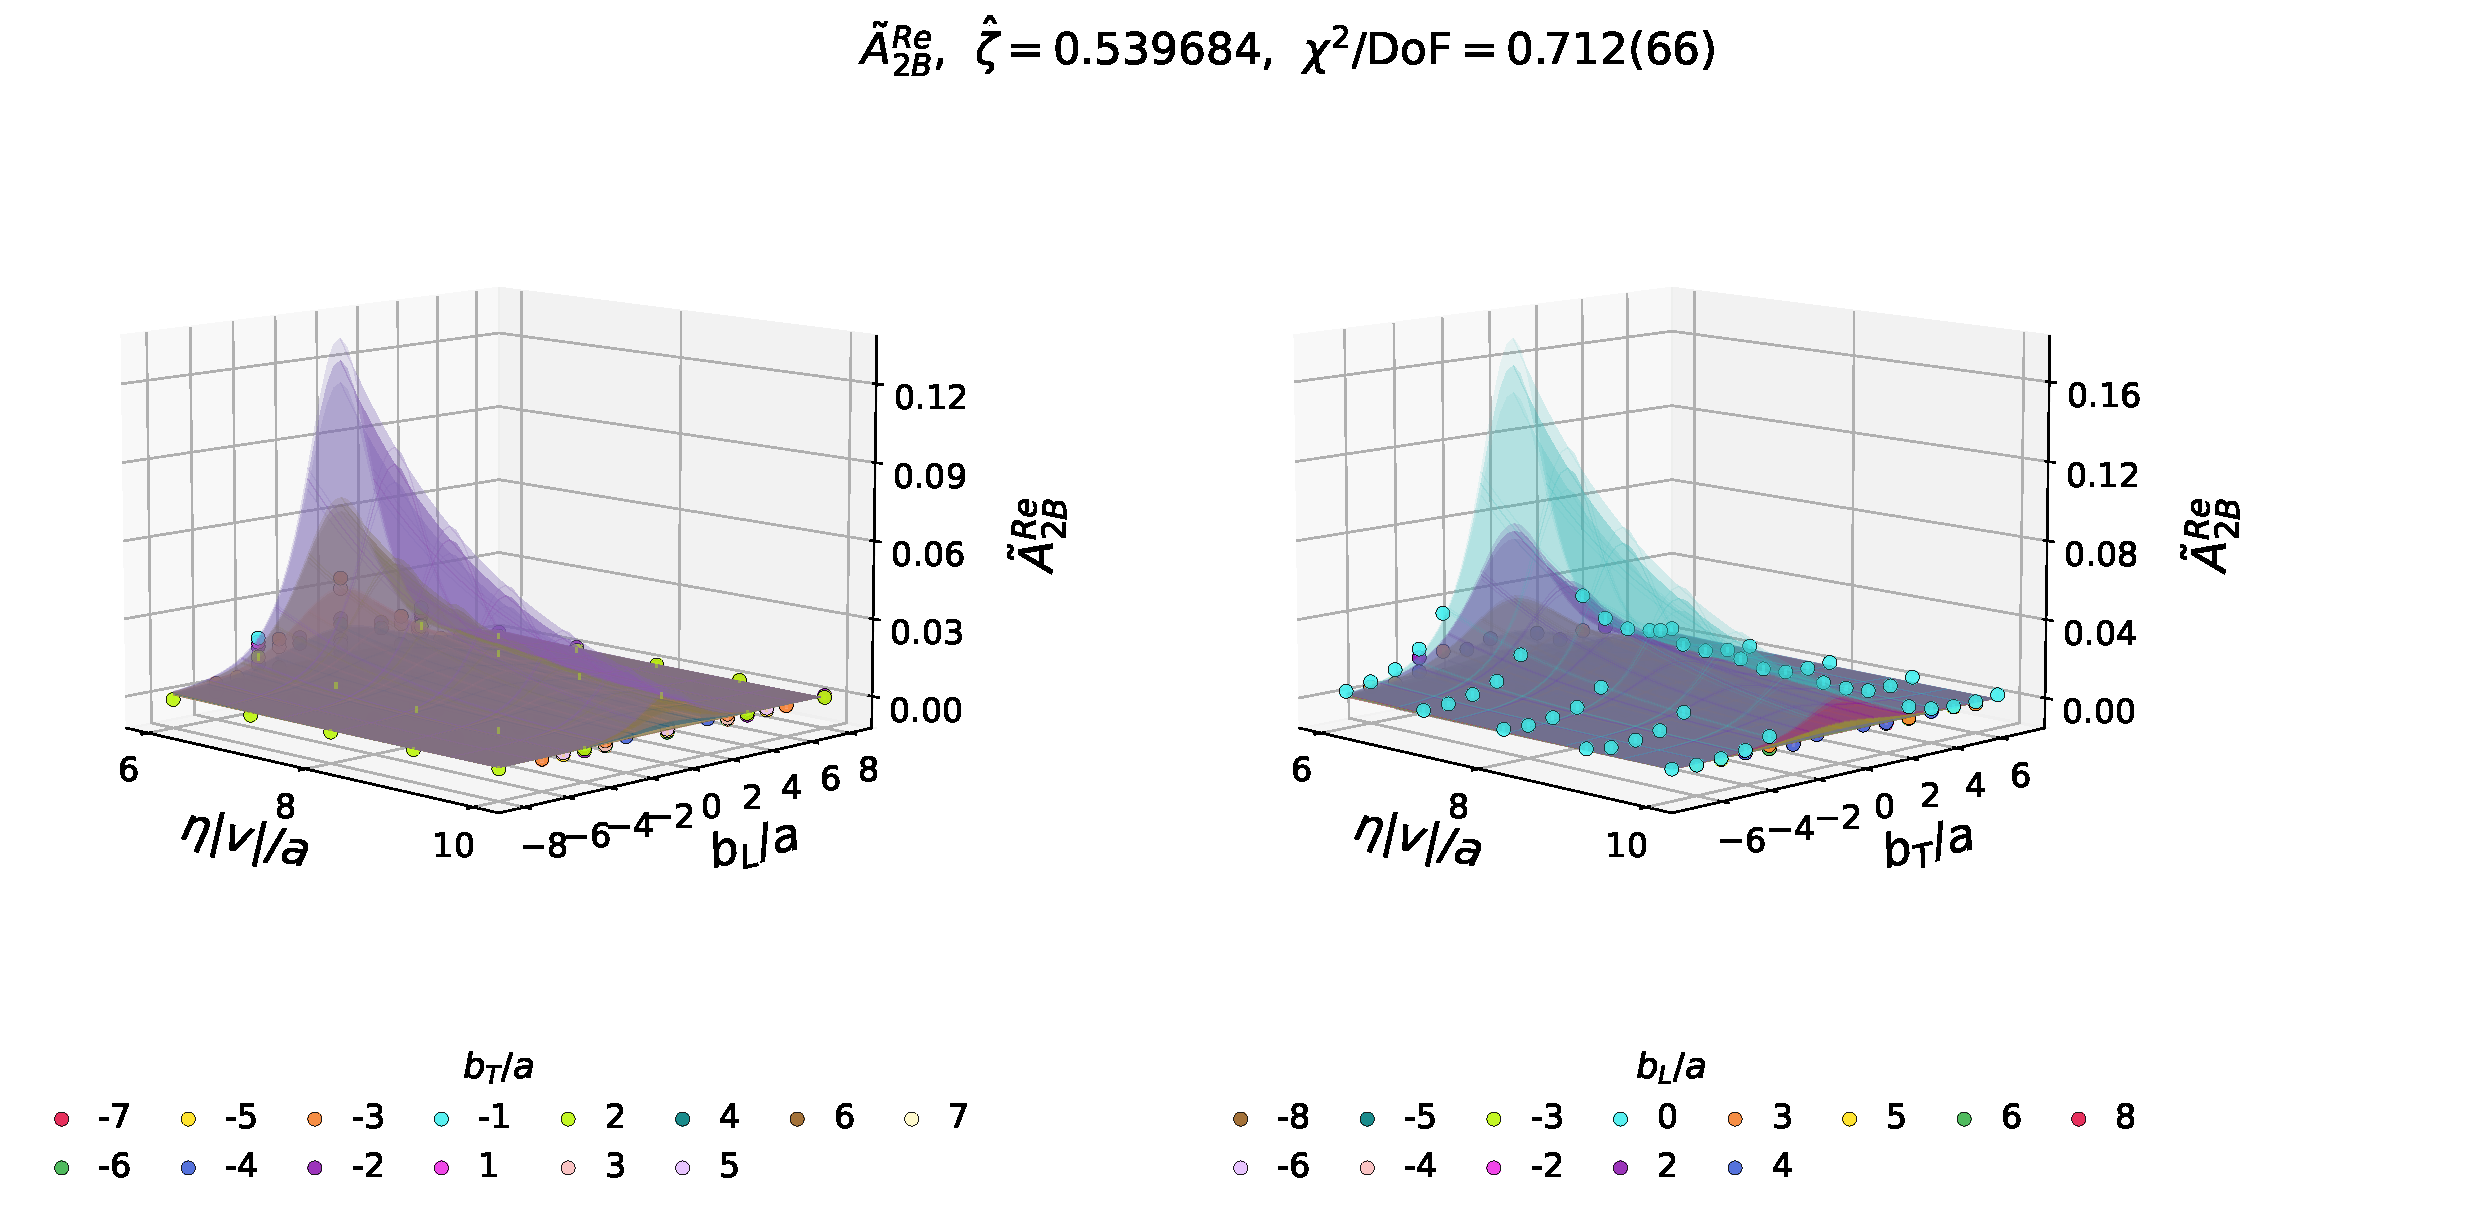
\includegraphics[width=\linewidth,height=.70\textheight,keepaspectratio]{fitting/ReA2B_PL-3_WithFit_3D.pdf}
\par\small Spatial coordinates: $(b_L,b_T,\eta)$. All panels and data overlays retained.

\figsrc{Thesis: plots; ReA2B\_PL-3\_WithFit\_3D}
\end{frame}

\begin{frame}{Global fit: $\tAmp_{2B}^{\mathrm{Re}}$, $P_L=-3$}
\centering
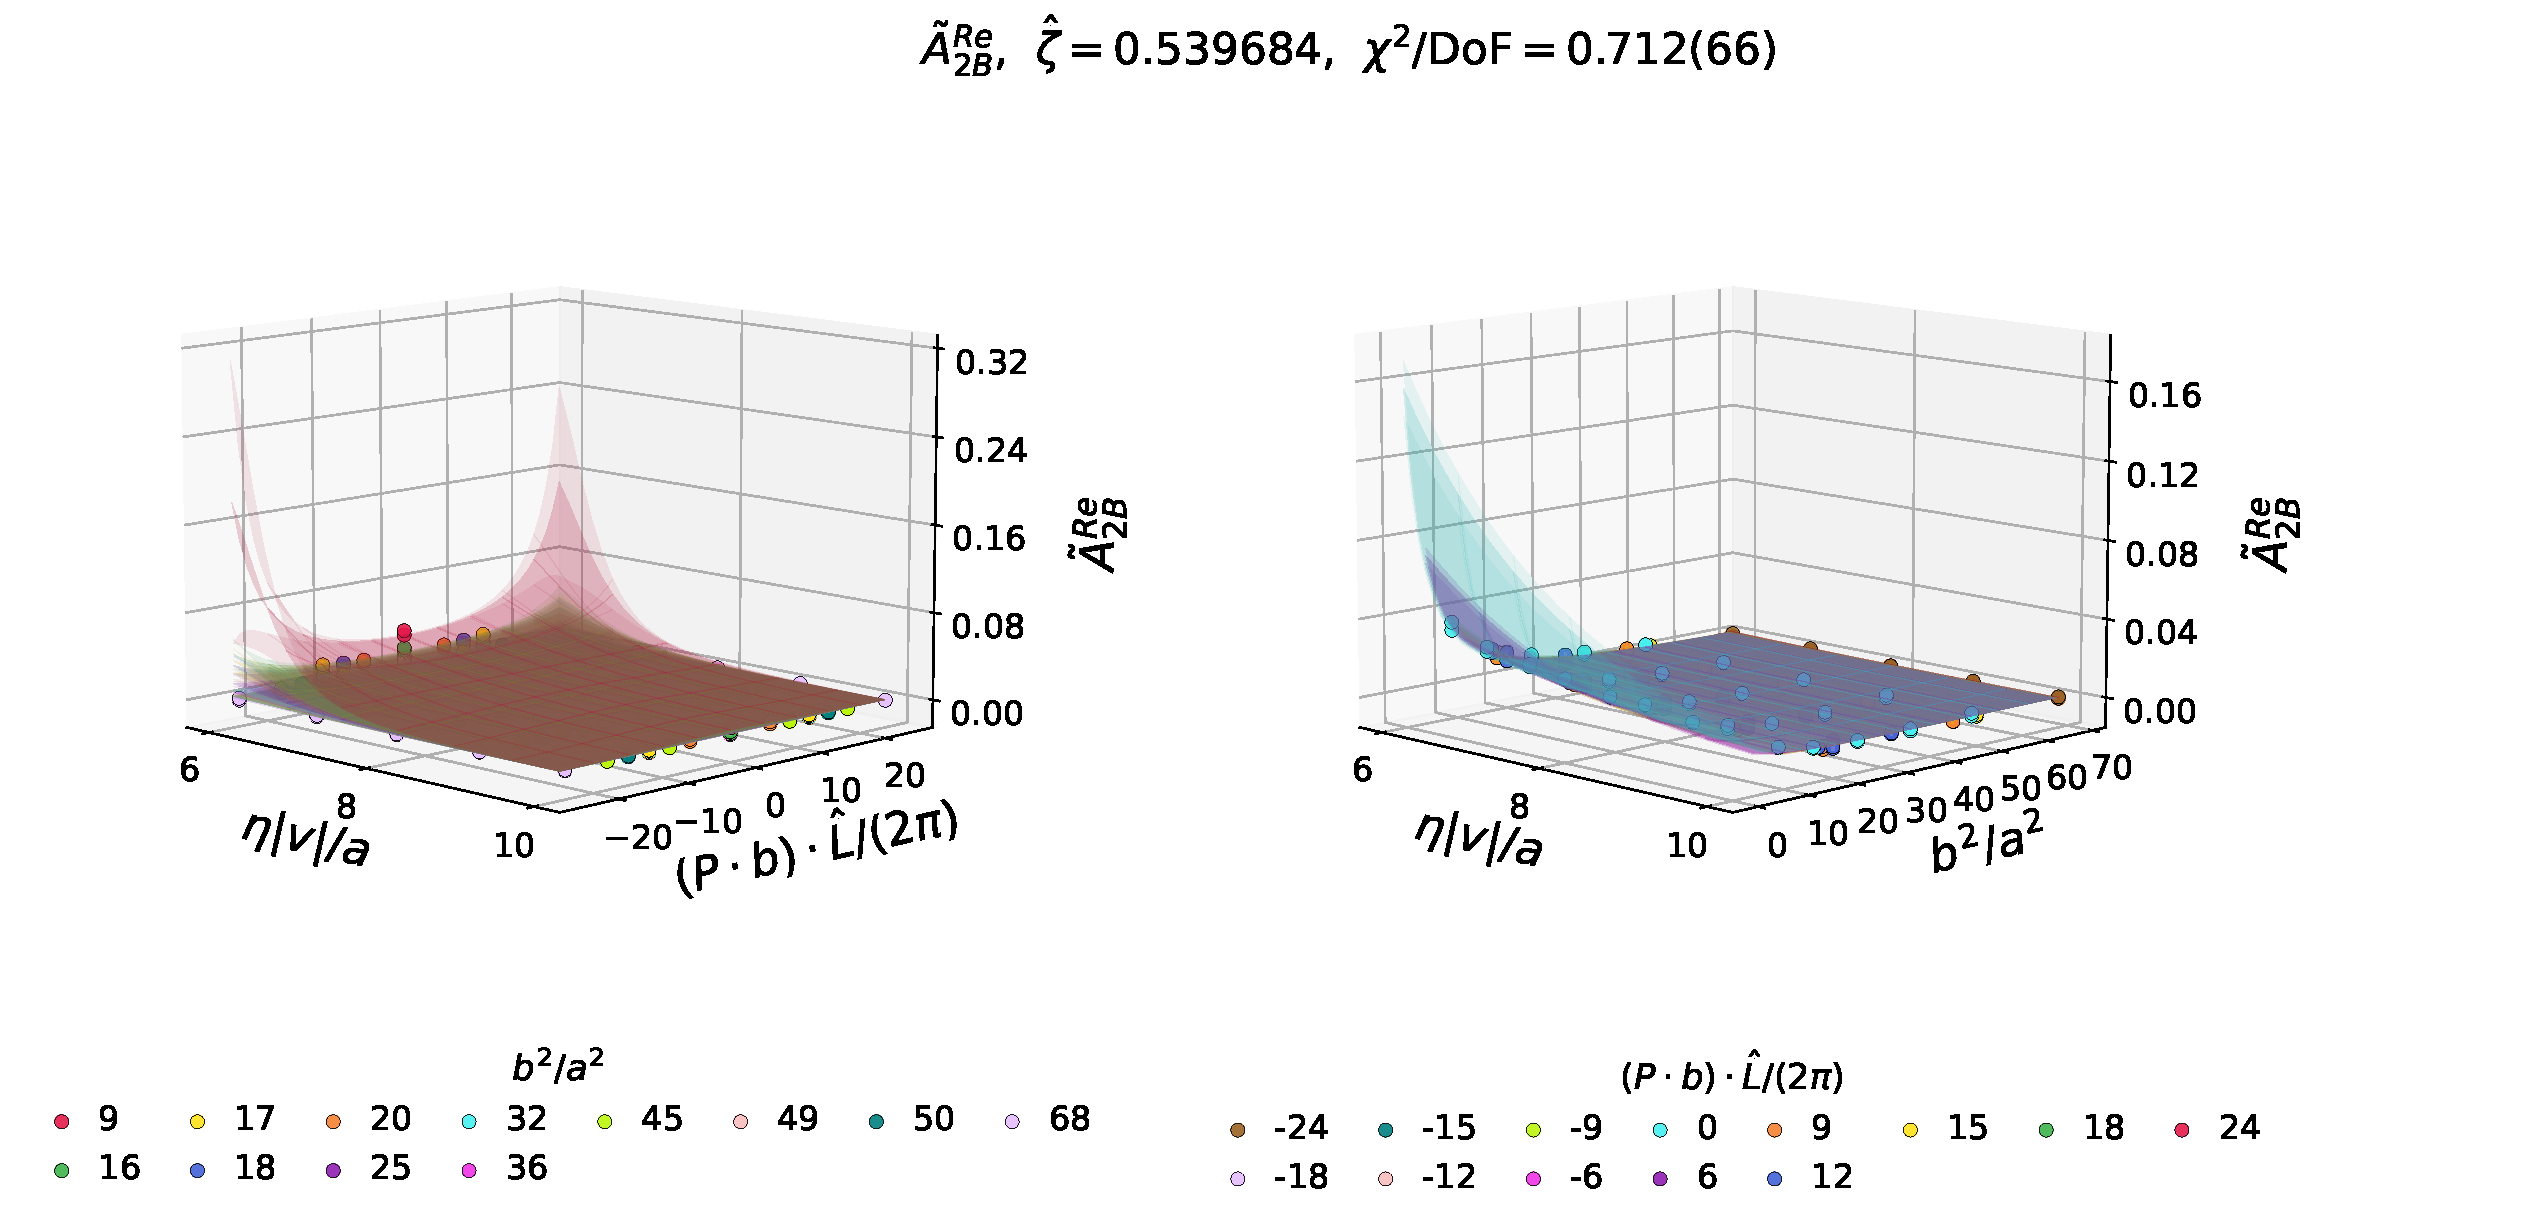
\includegraphics[width=\linewidth,height=.70\textheight,keepaspectratio]{fitting/ReA2B_Pb_bsq_PL-3_WithFit_3D.pdf}
\par\small Invariant coordinates: $(\nu,b^2,\eta)$. All panels and data overlays retained.

\figsrc{Thesis: plots; ReA2B\_Pb\_bsq\_PL-3\_WithFit\_3D}
\end{frame}

\begin{frame}{Fixed staple $\eta=8$: $\tAmp_{2B}^{\mathrm{Re}}$, $P_L=-3$}
\centering
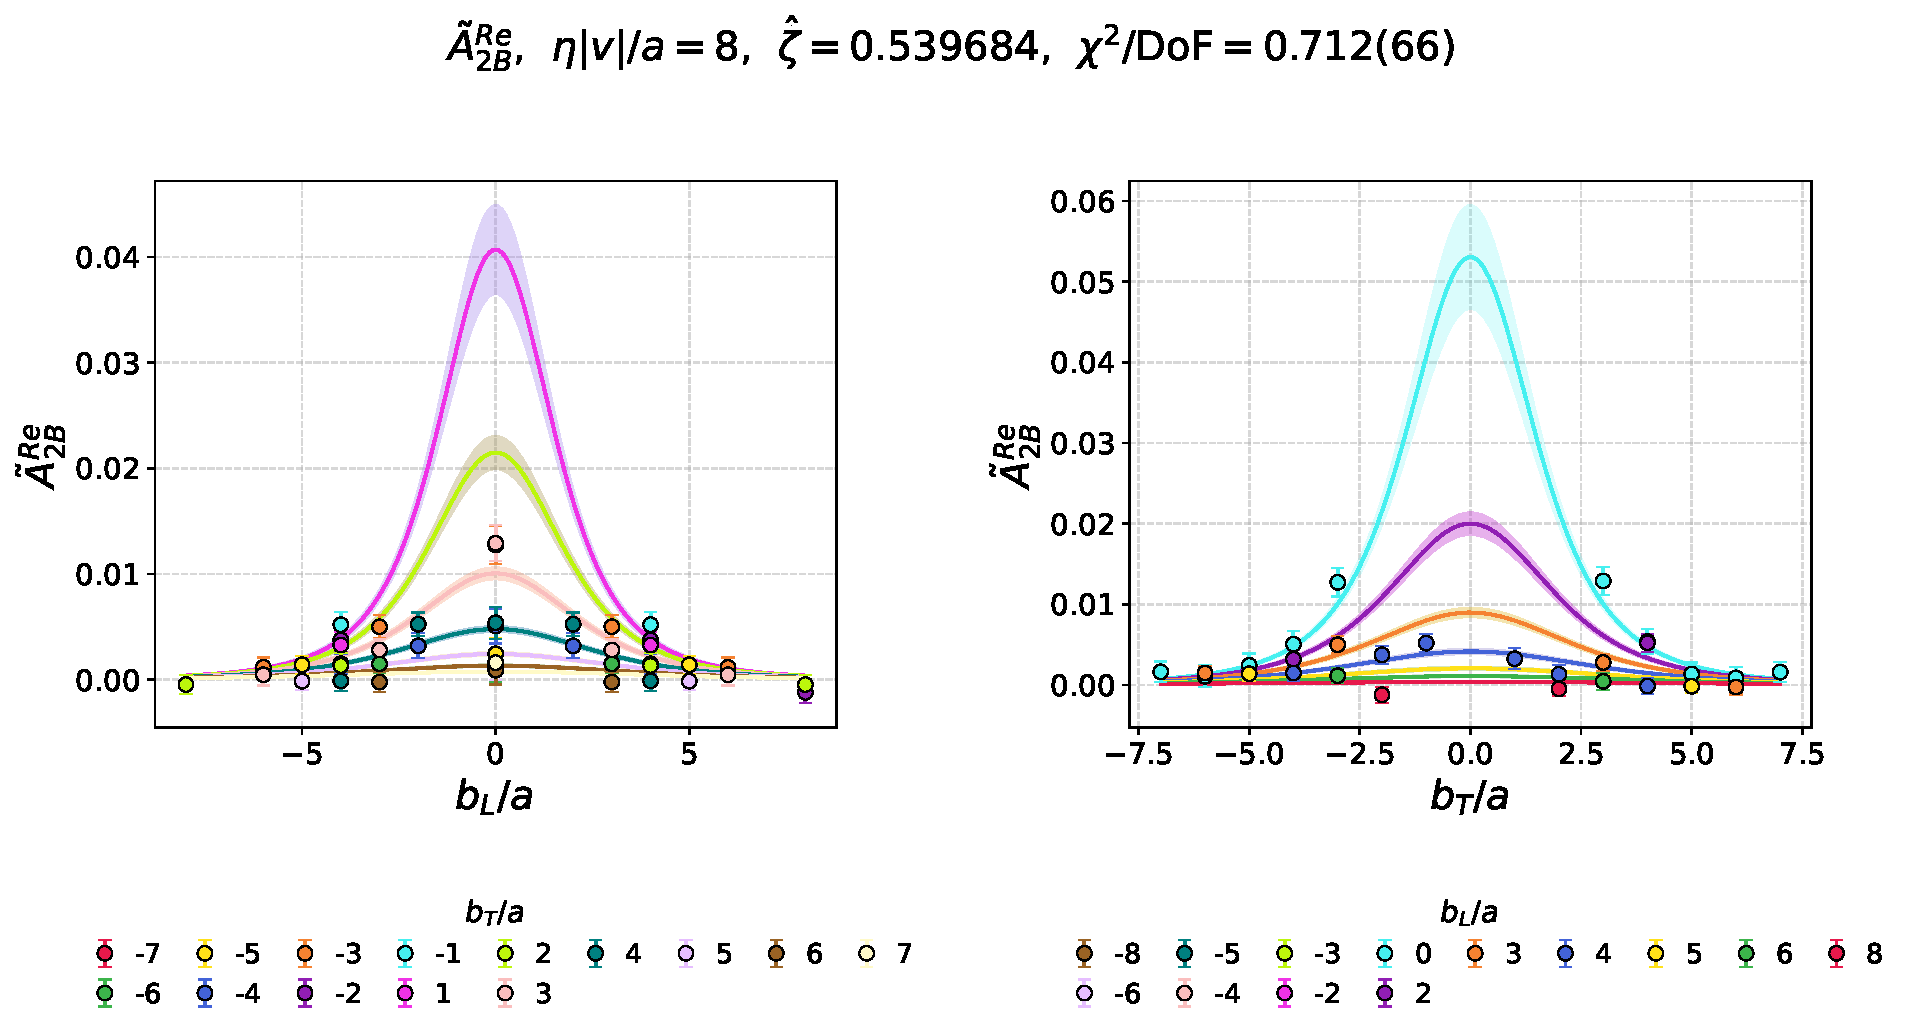
\includegraphics[width=\linewidth,height=.70\textheight,keepaspectratio]{fitting/ReA2B_eta8_PL-3_WithFit_2D.pdf}
\par\small Both spatial-coordinate slices. Same simultaneous fit, with Jackknife bands.

\figsrc{Thesis: plots; ReA2B\_eta8\_PL-3\_WithFit\_2D}
\end{frame}

\begin{frame}{Fixed staple $\eta=8$: $\tAmp_{2B}^{\mathrm{Re}}$, $P_L=-3$}
\centering
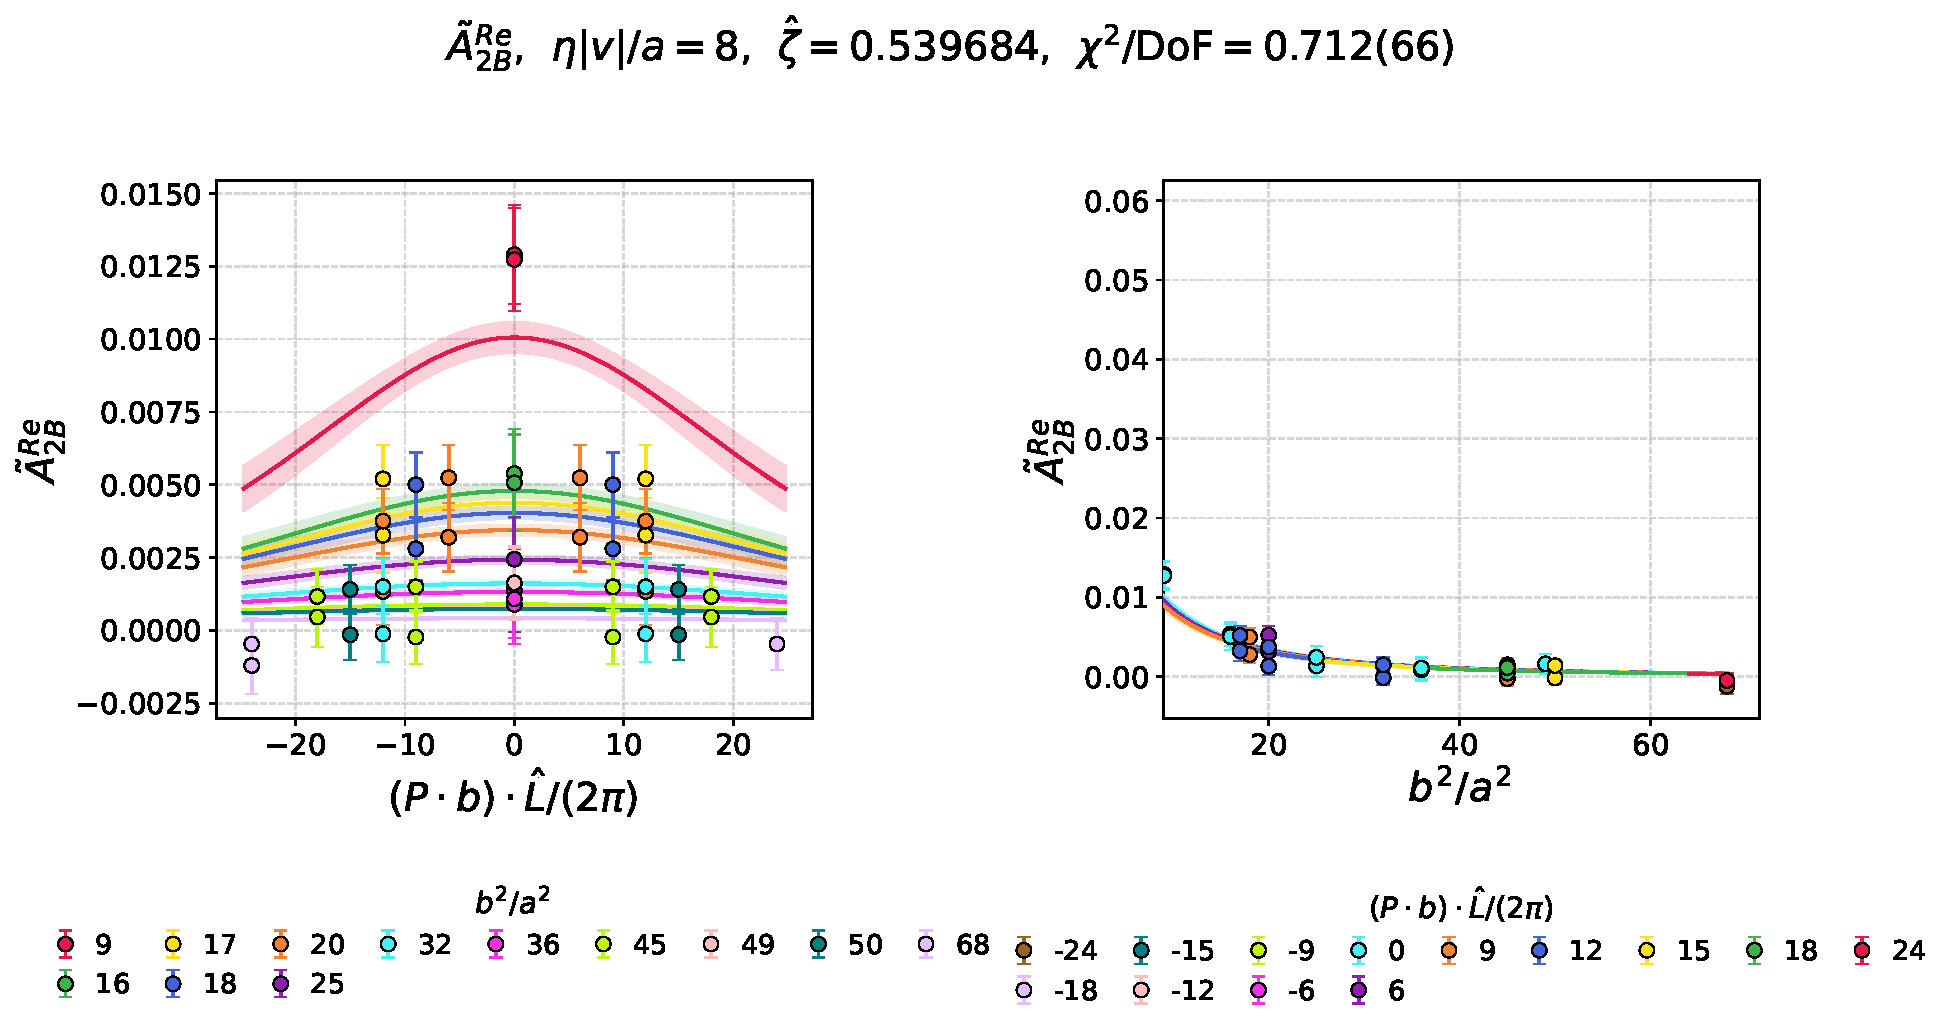
\includegraphics[width=\linewidth,height=.70\textheight,keepaspectratio]{fitting/ReA2B_Pb_bsq_eta8_PL-3_WithFit_2D.pdf}
\par\small Both invariant-coordinate slices. Same simultaneous fit, with Jackknife bands.

\figsrc{Thesis: plots; ReA2B\_Pb\_bsq\_eta8\_PL-3\_WithFit\_2D}
\end{frame}

\begin{frame}{Global fit: $\tAmp_{2B}^{\mathrm{Im}}$, $P_L=-3$}
\centering
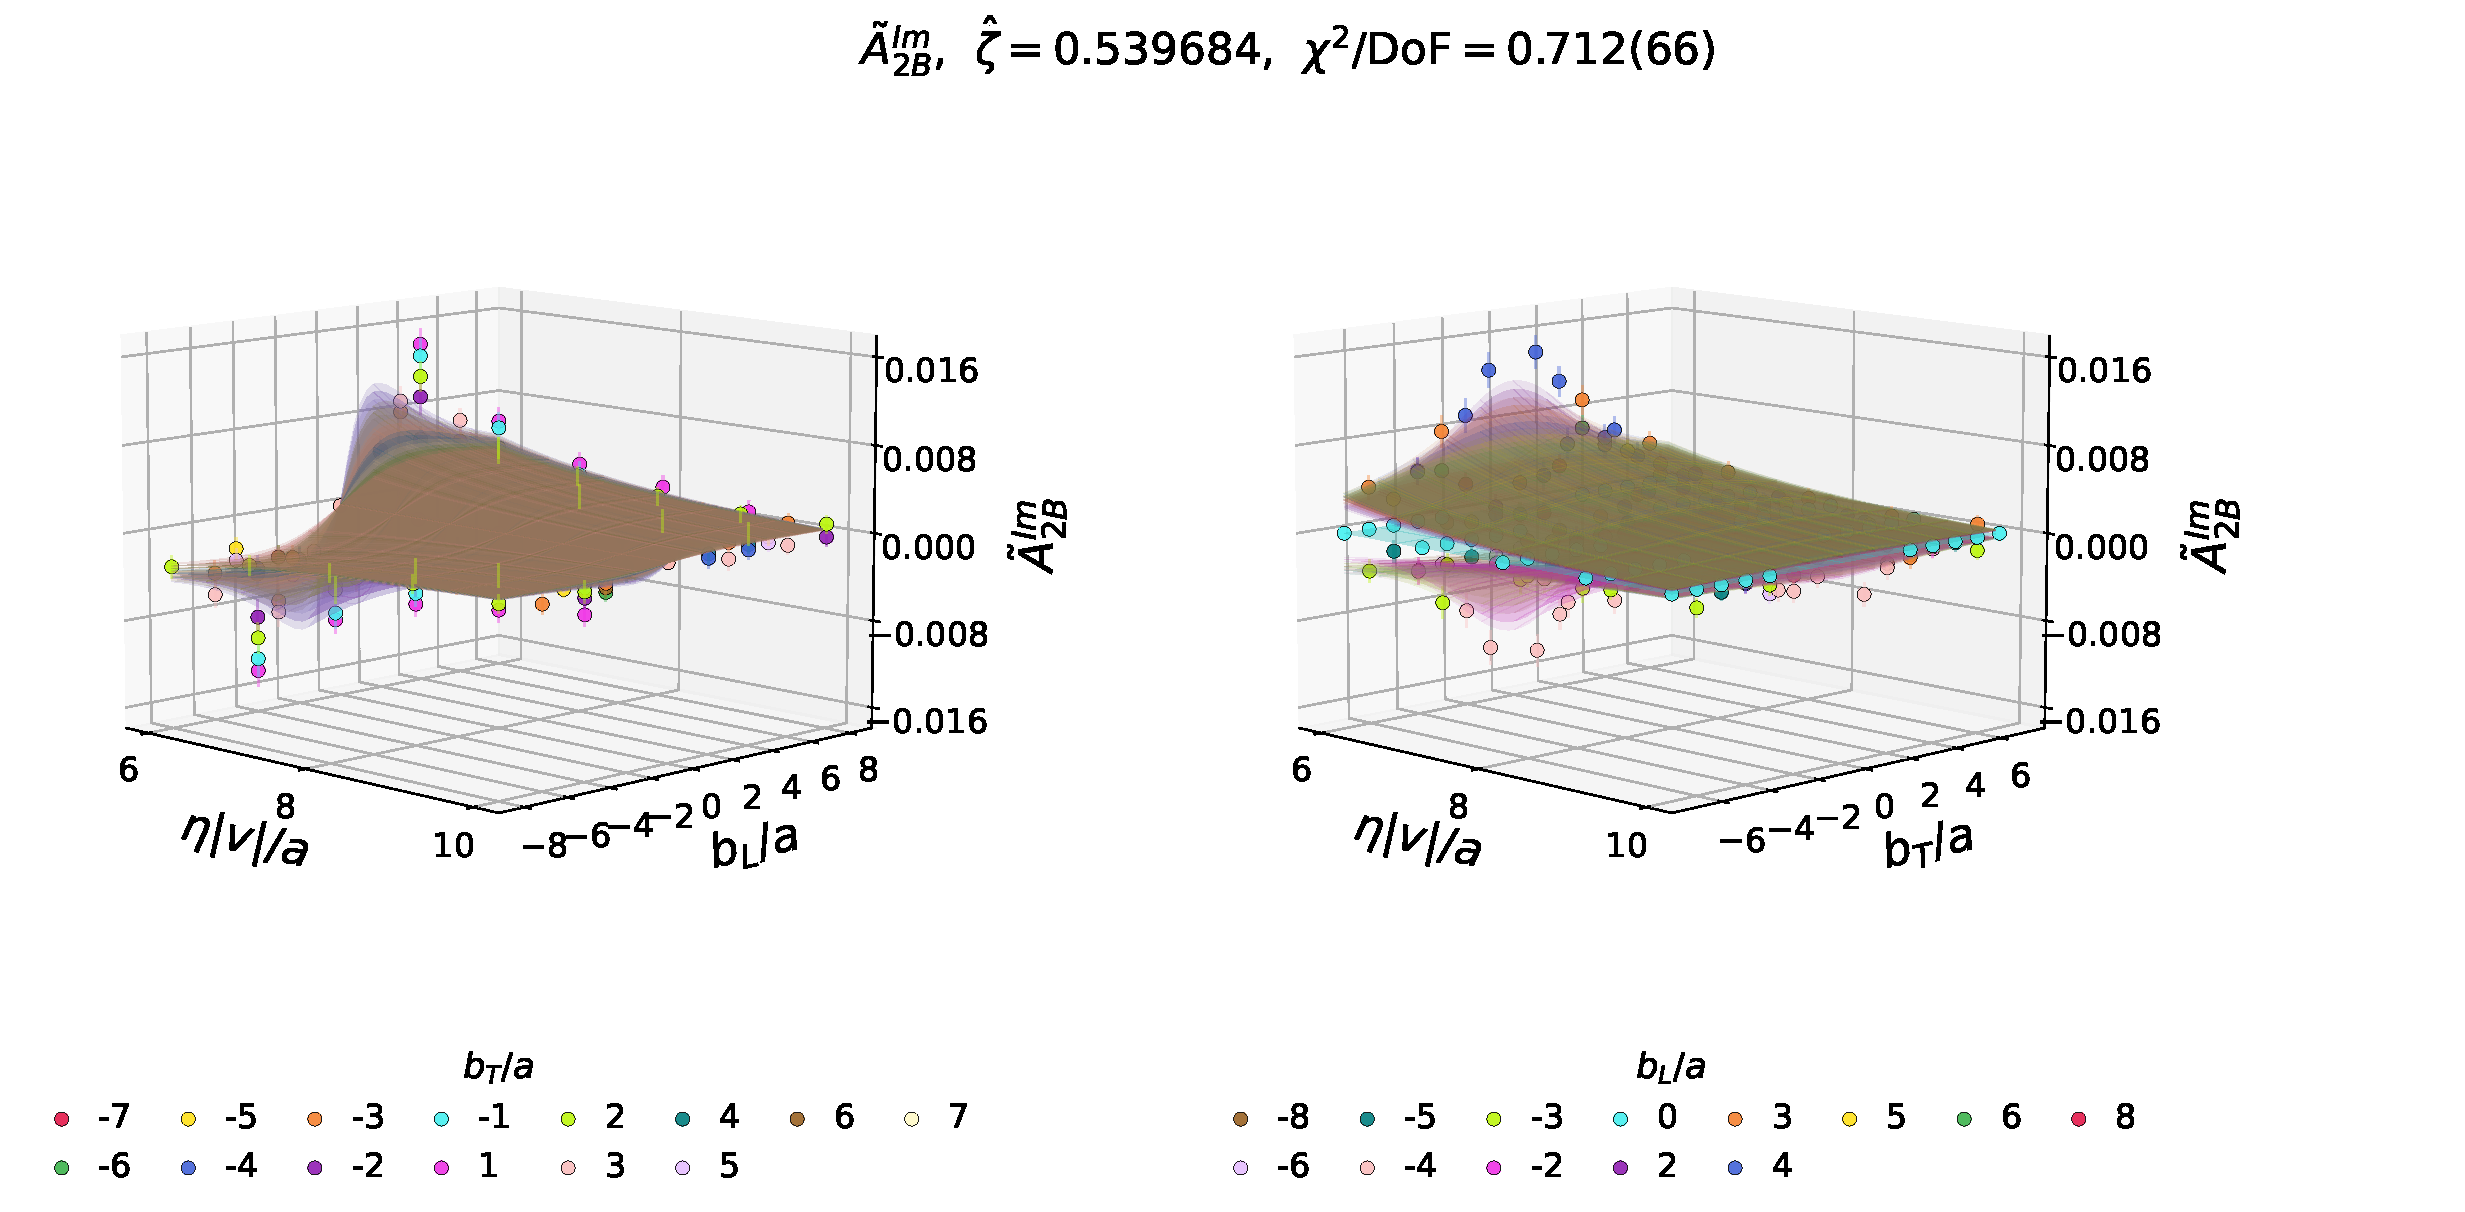
\includegraphics[width=\linewidth,height=.70\textheight,keepaspectratio]{fitting/ImA2B_PL-3_WithFit_3D.pdf}
\par\small Spatial coordinates: $(b_L,b_T,\eta)$. All panels and data overlays retained.

\figsrc{Thesis: plots; ImA2B\_PL-3\_WithFit\_3D}
\end{frame}

\begin{frame}{Global fit: $\tAmp_{2B}^{\mathrm{Im}}$, $P_L=-3$}
\centering
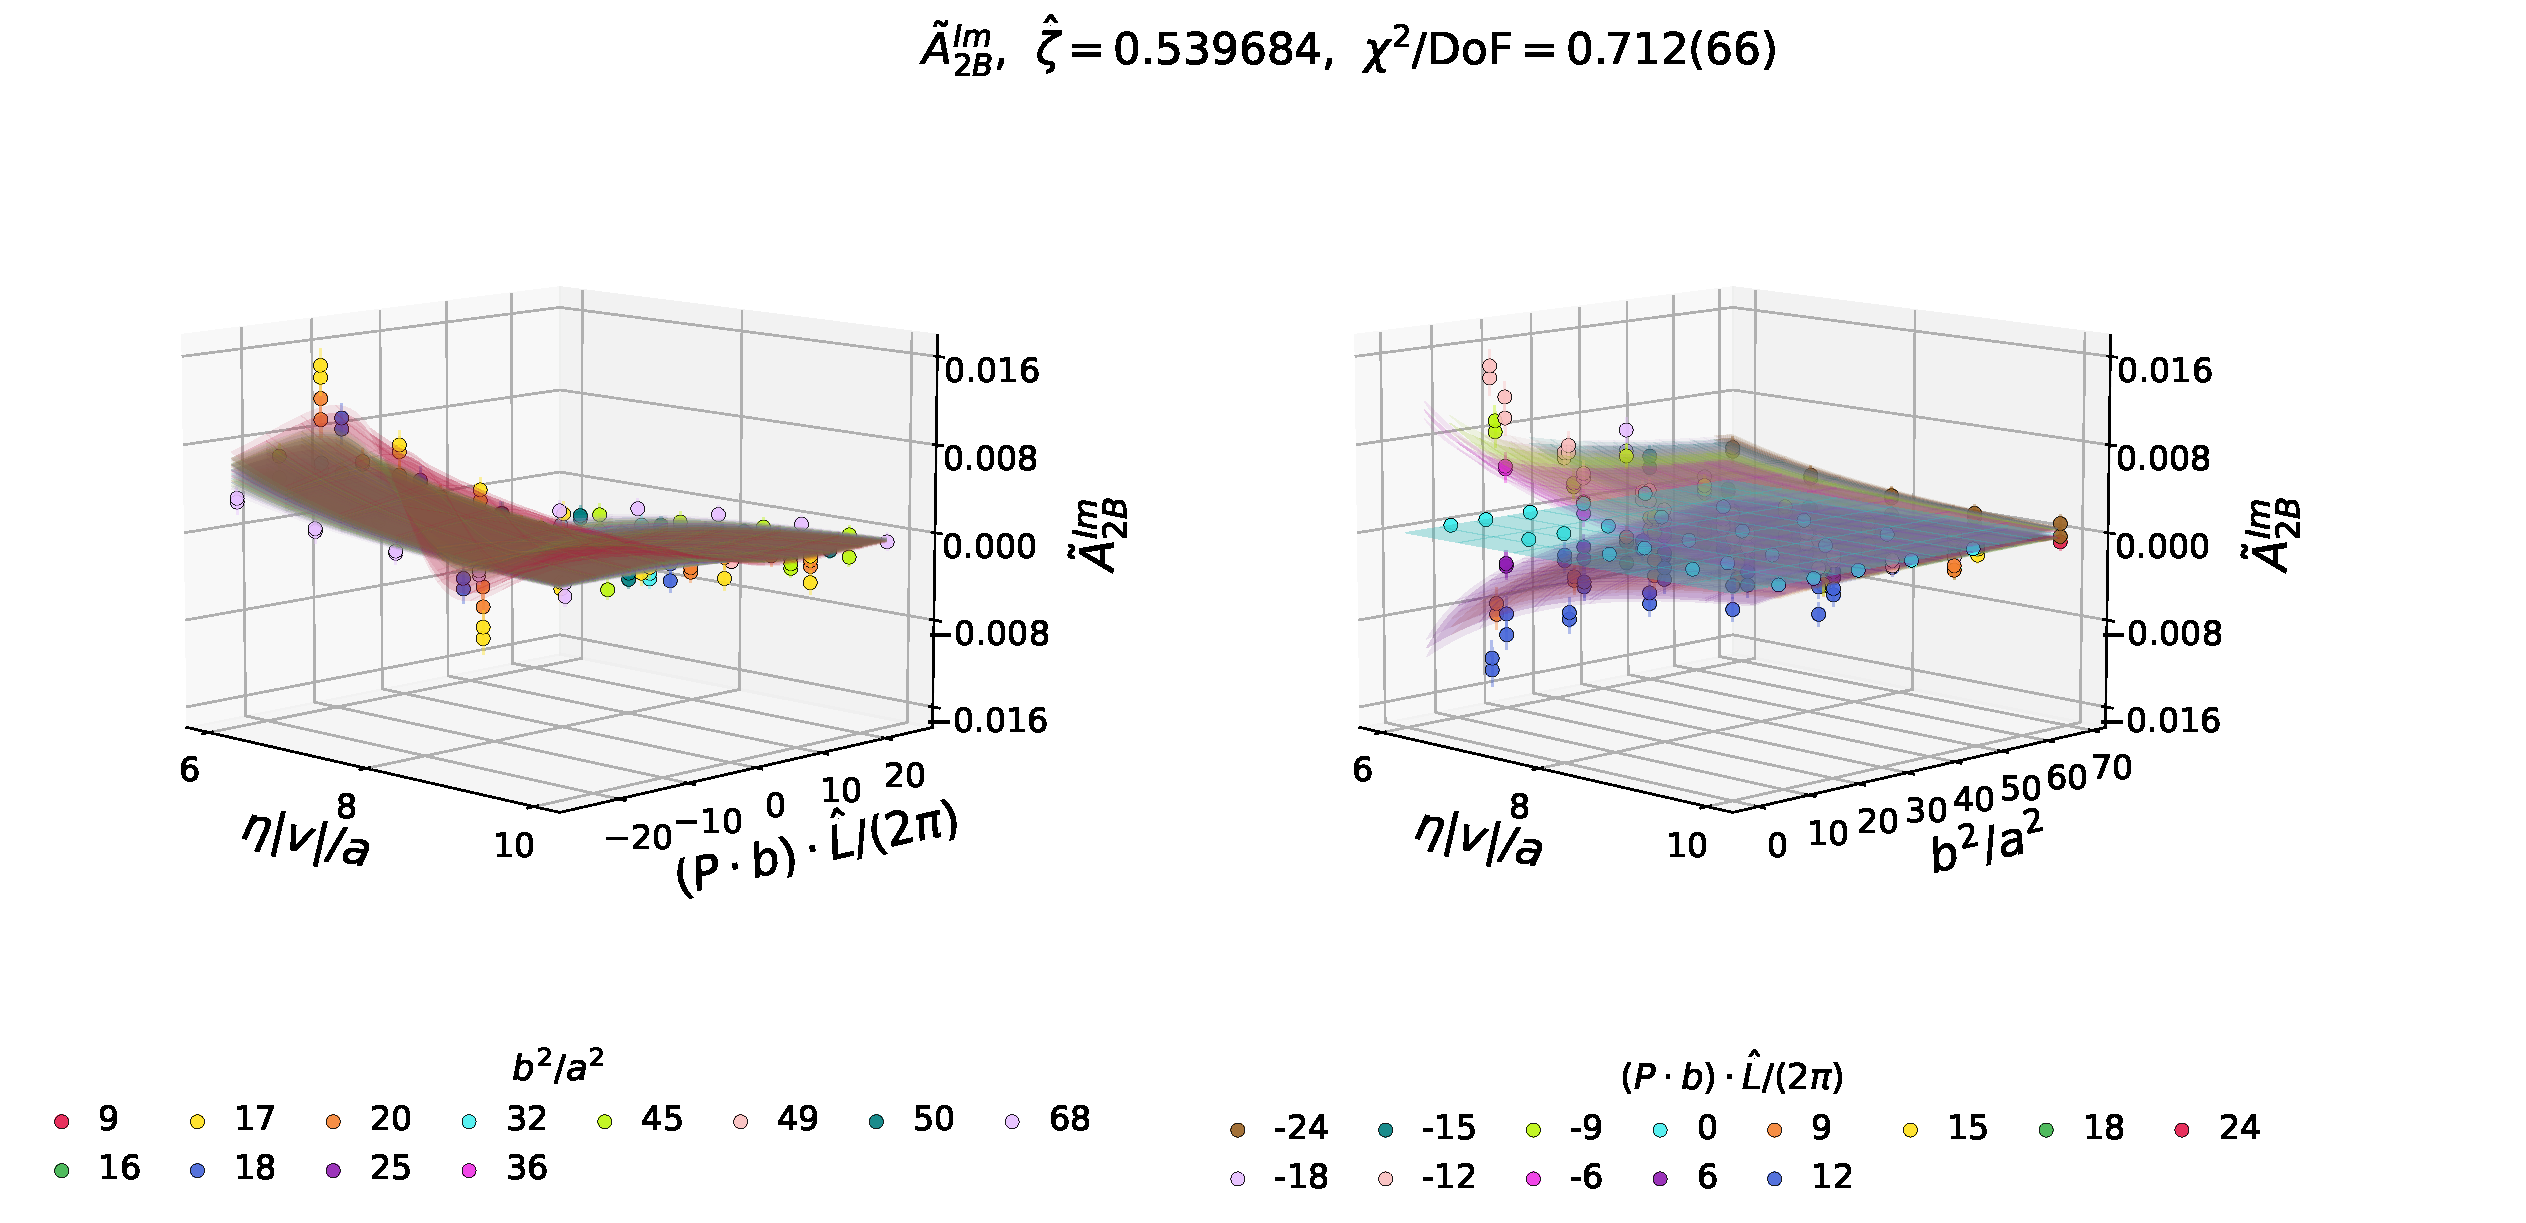
\includegraphics[width=\linewidth,height=.70\textheight,keepaspectratio]{fitting/ImA2B_Pb_bsq_PL-3_WithFit_3D.pdf}
\par\small Invariant coordinates: $(\nu,b^2,\eta)$. All panels and data overlays retained.

\figsrc{Thesis: plots; ImA2B\_Pb\_bsq\_PL-3\_WithFit\_3D}
\end{frame}

\begin{frame}{Fixed staple $\eta=8$: $\tAmp_{2B}^{\mathrm{Im}}$, $P_L=-3$}
\centering
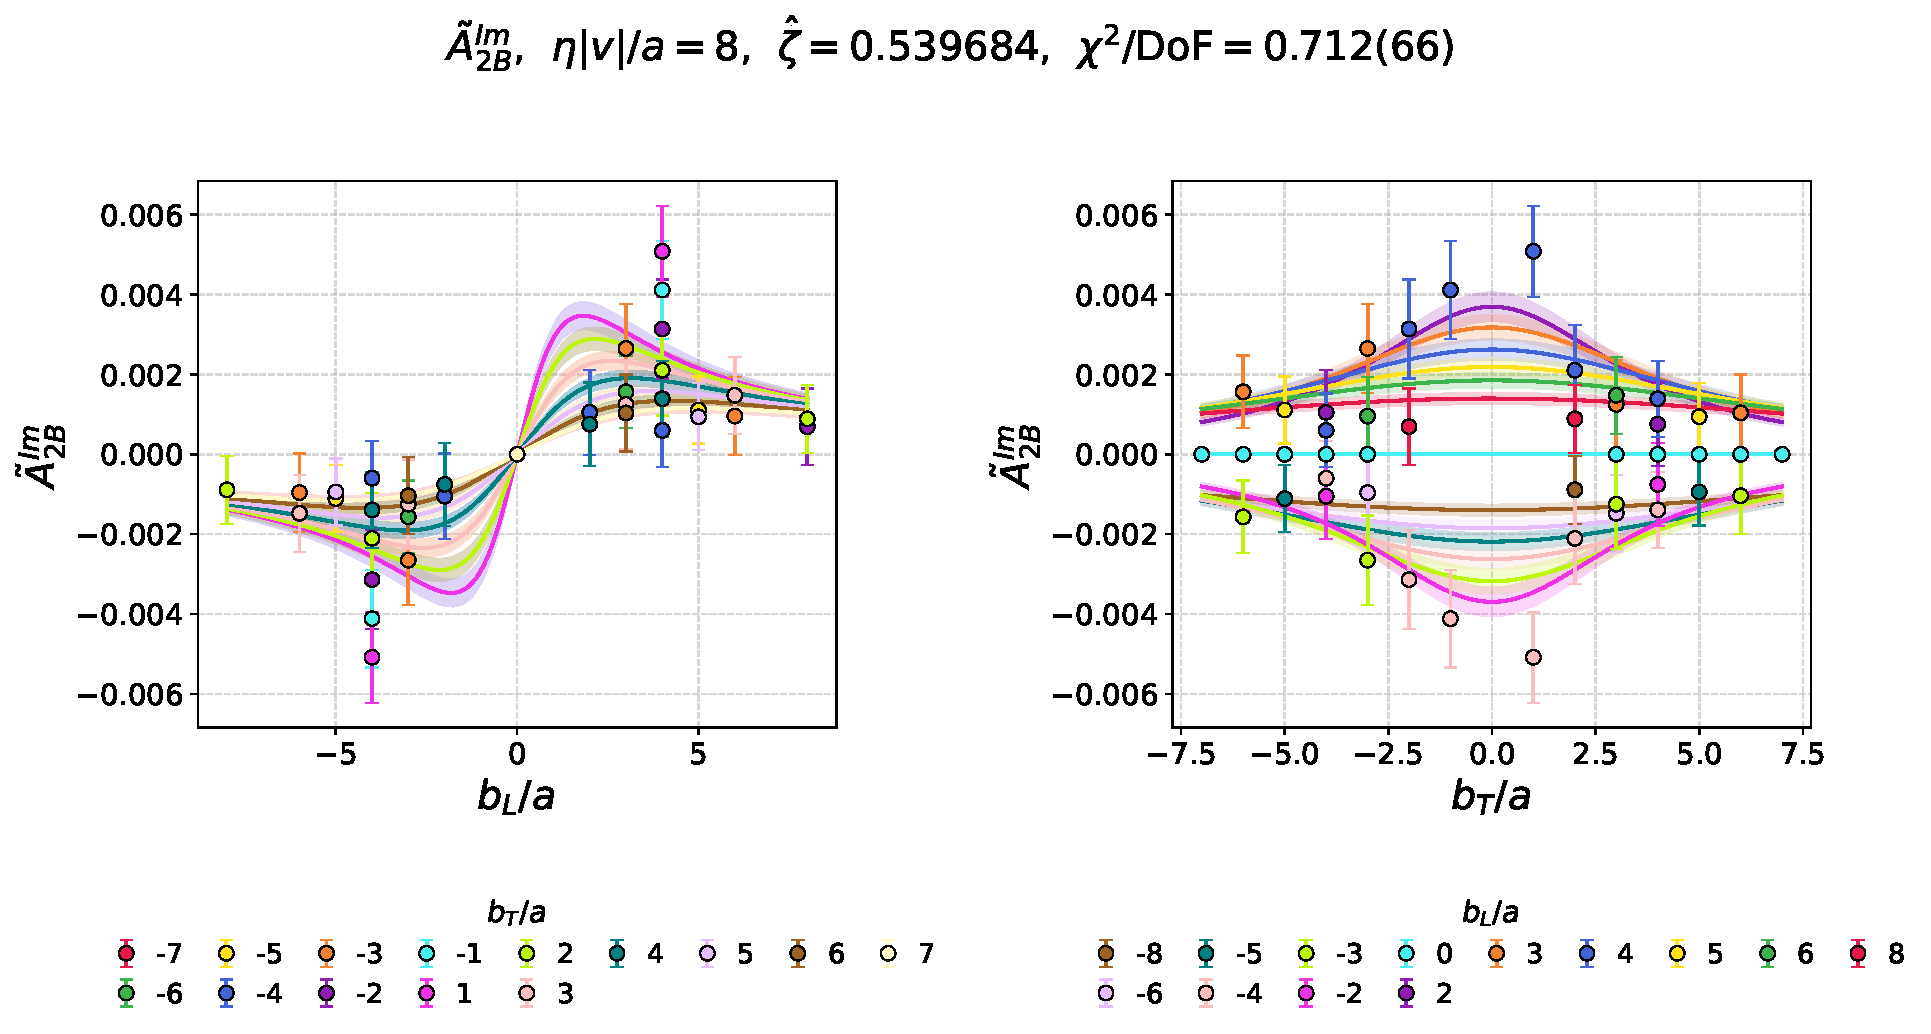
\includegraphics[width=\linewidth,height=.70\textheight,keepaspectratio]{fitting/ImA2B_eta8_PL-3_WithFit_2D.pdf}
\par\small Both spatial-coordinate slices. Same simultaneous fit, with Jackknife bands.

\figsrc{Thesis: plots; ImA2B\_eta8\_PL-3\_WithFit\_2D}
\end{frame}

\begin{frame}{Fixed staple $\eta=8$: $\tAmp_{2B}^{\mathrm{Im}}$, $P_L=-3$}
\centering
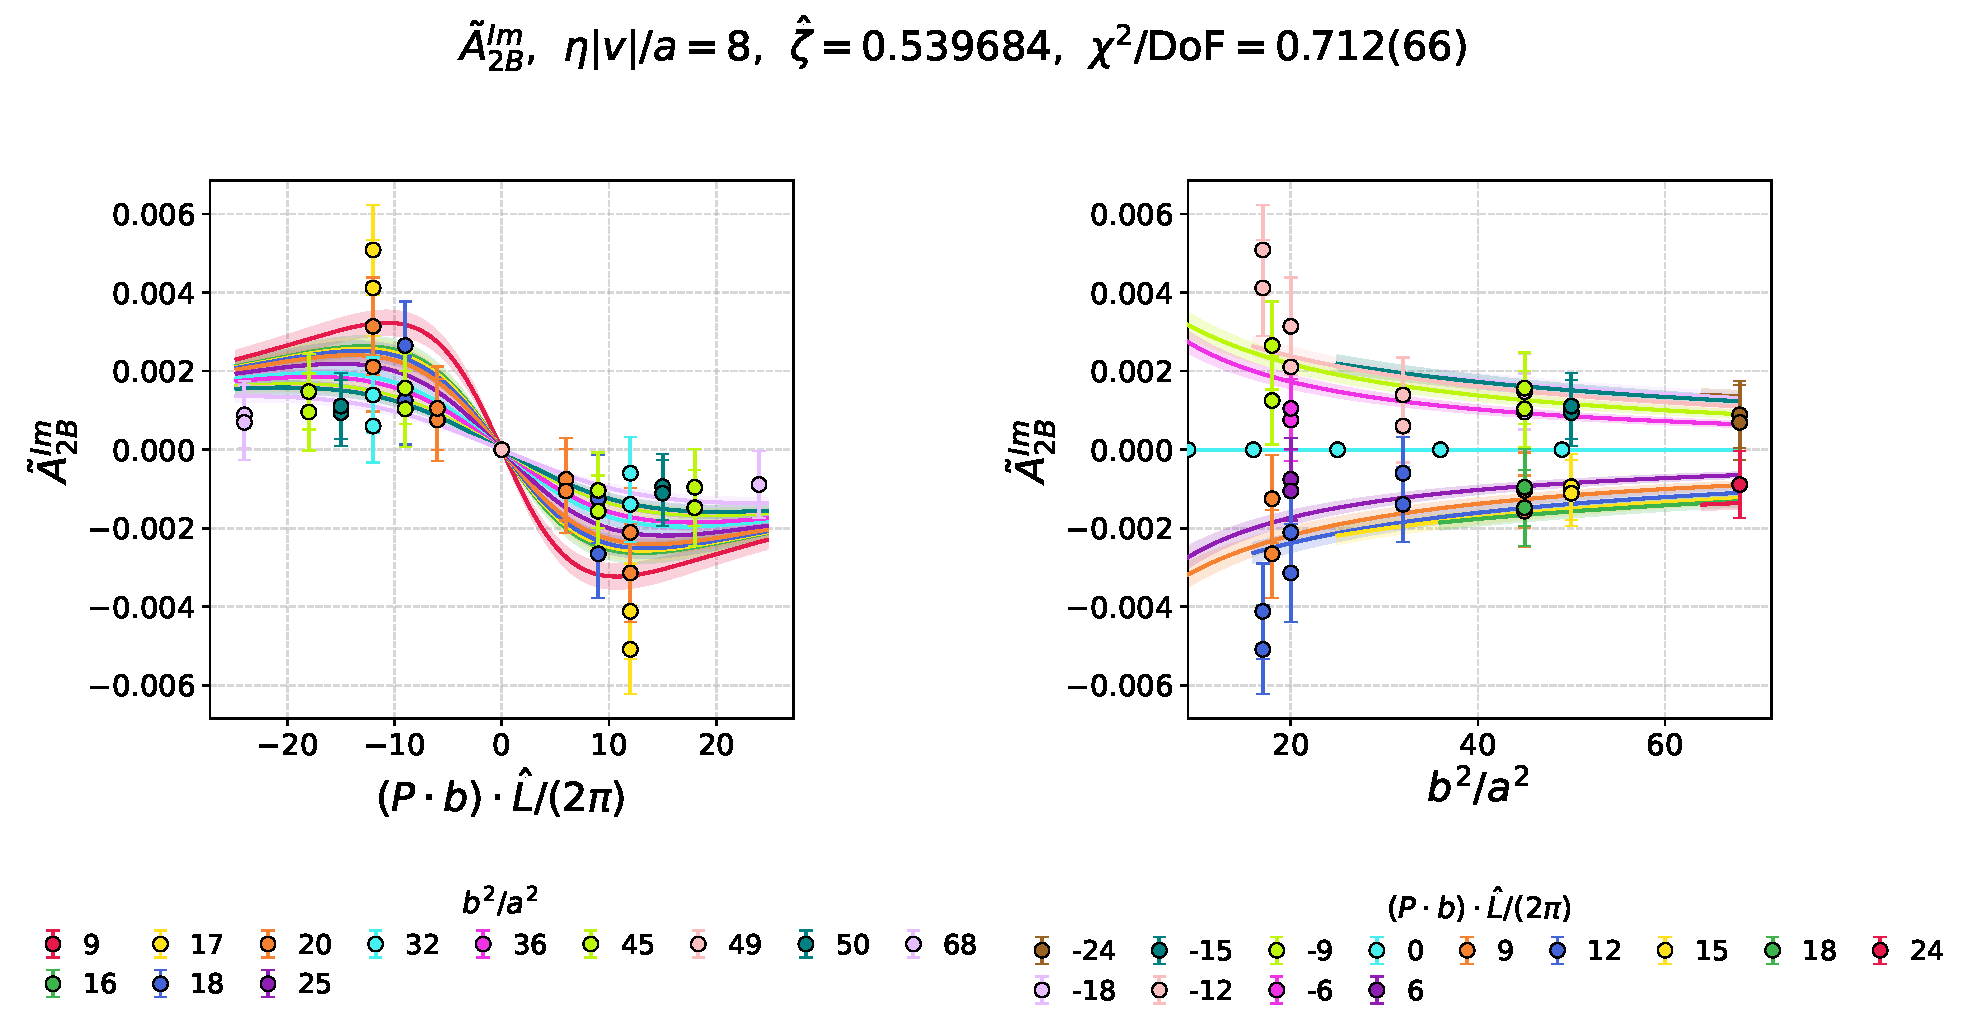
\includegraphics[width=\linewidth,height=.70\textheight,keepaspectratio]{fitting/ImA2B_Pb_bsq_eta8_PL-3_WithFit_2D.pdf}
\par\small Both invariant-coordinate slices. Same simultaneous fit, with Jackknife bands.

\figsrc{Thesis: plots; ImA2B\_Pb\_bsq\_eta8\_PL-3\_WithFit\_2D}
\end{frame}

\begin{frame}{Global fit: $\tAmp_{12B}^{\mathrm{Re}}$, $P_L=-3$}
\centering
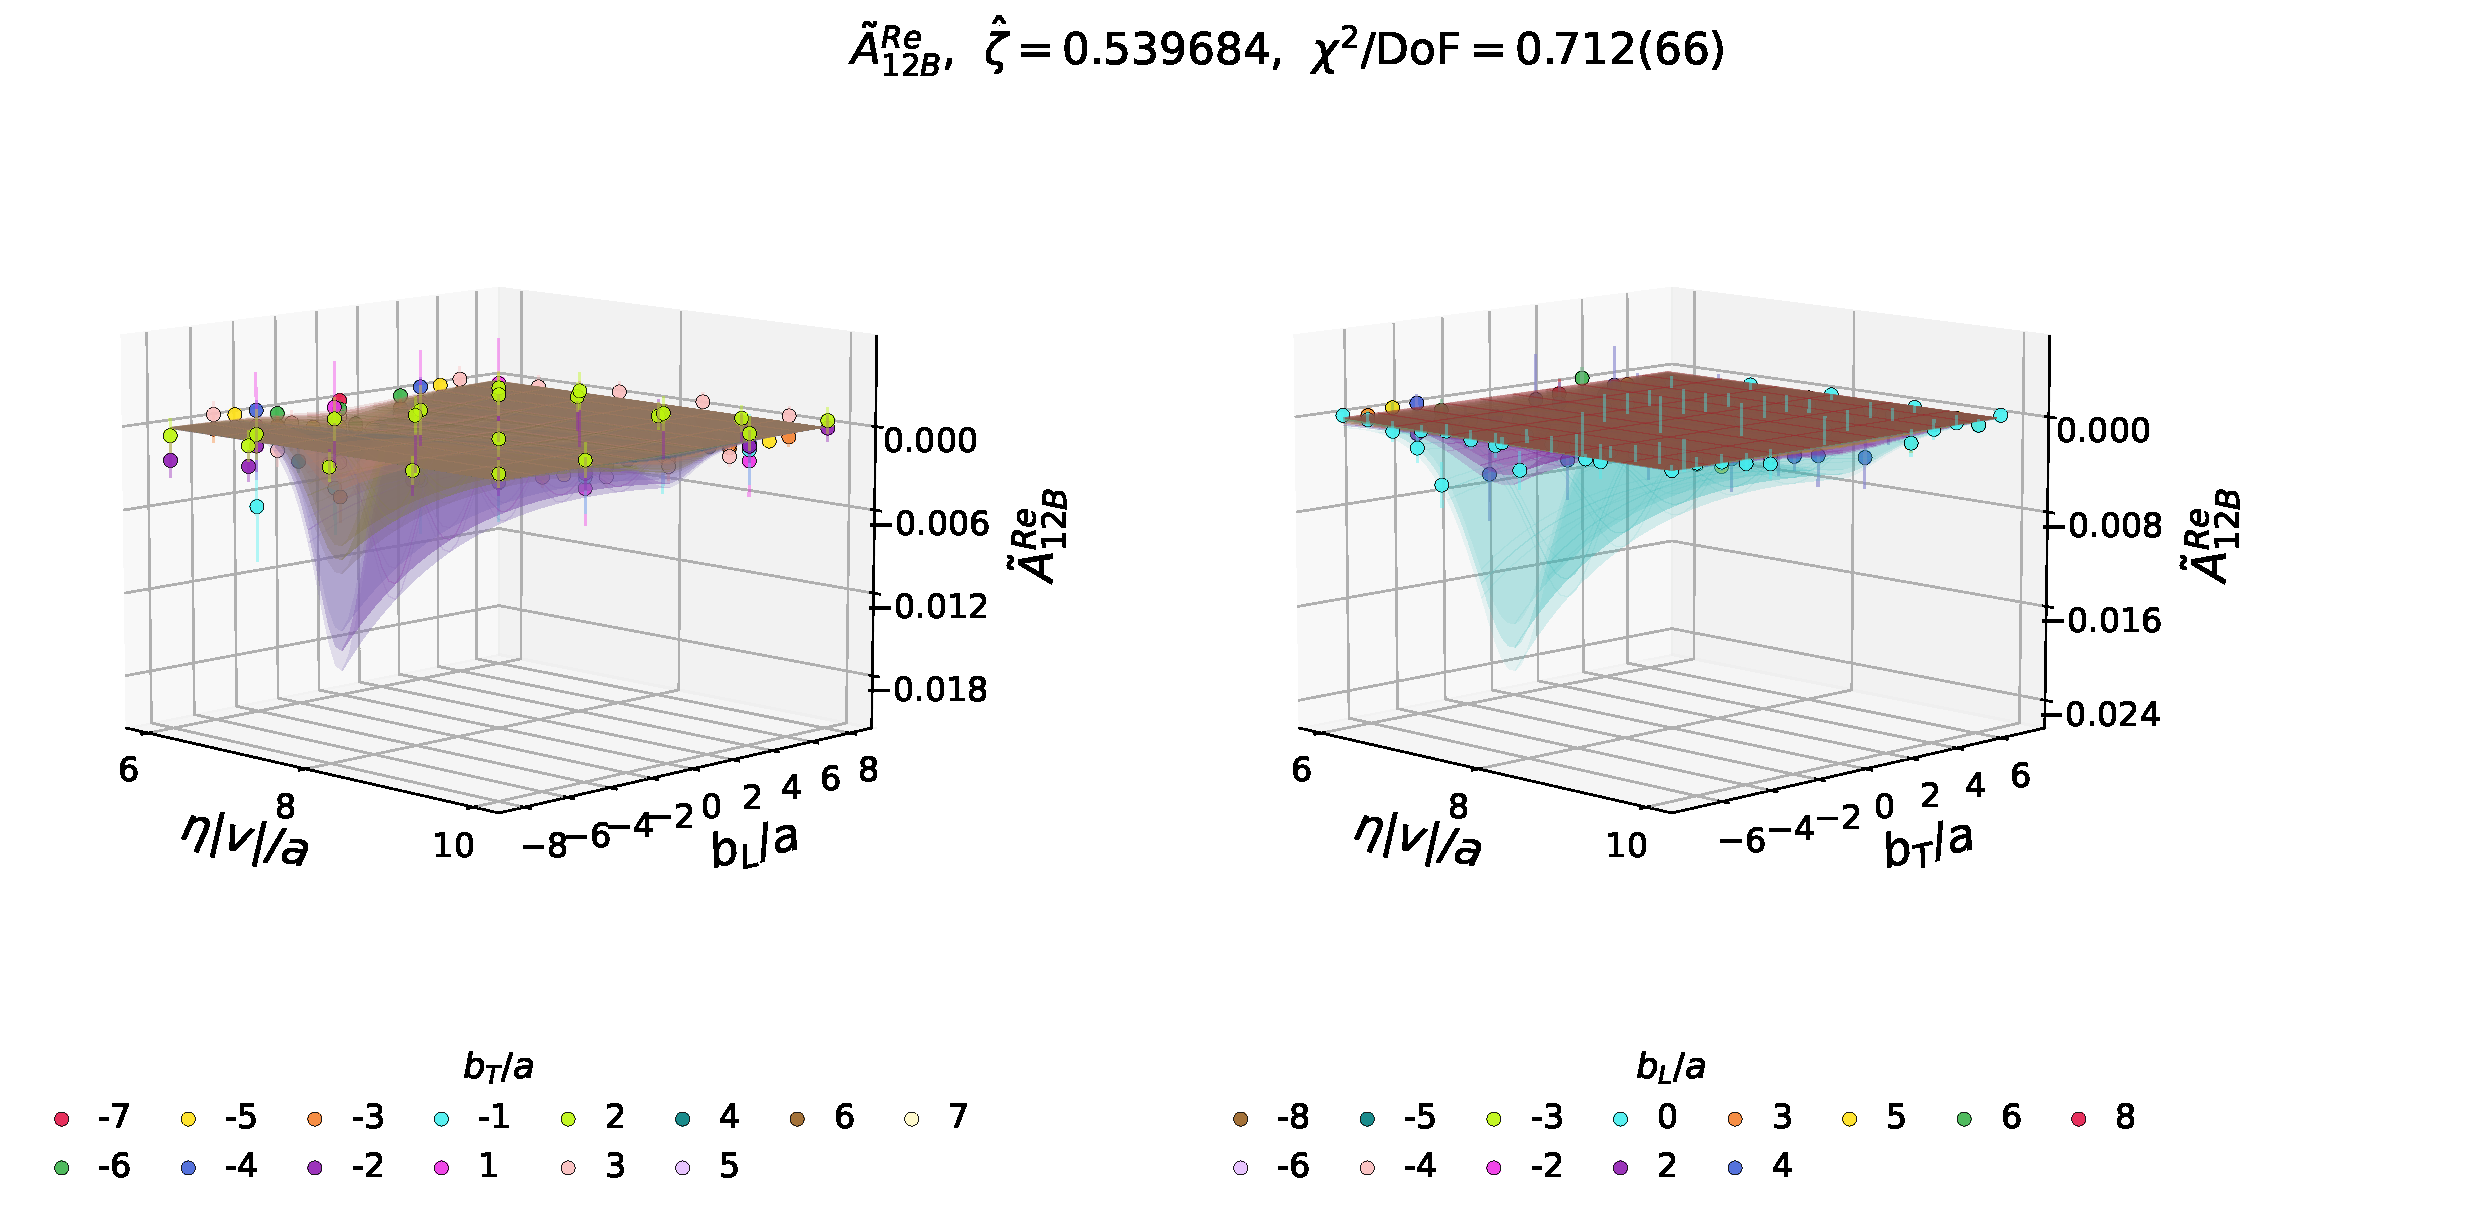
\includegraphics[width=\linewidth,height=.70\textheight,keepaspectratio]{fitting/ReA12B_PL-3_WithFit_3D.pdf}
\par\small Spatial coordinates: $(b_L,b_T,\eta)$. All panels and data overlays retained.

\figsrc{Thesis: plots; ReA12B\_PL-3\_WithFit\_3D}
\end{frame}

\begin{frame}{Global fit: $\tAmp_{12B}^{\mathrm{Re}}$, $P_L=-3$}
\centering
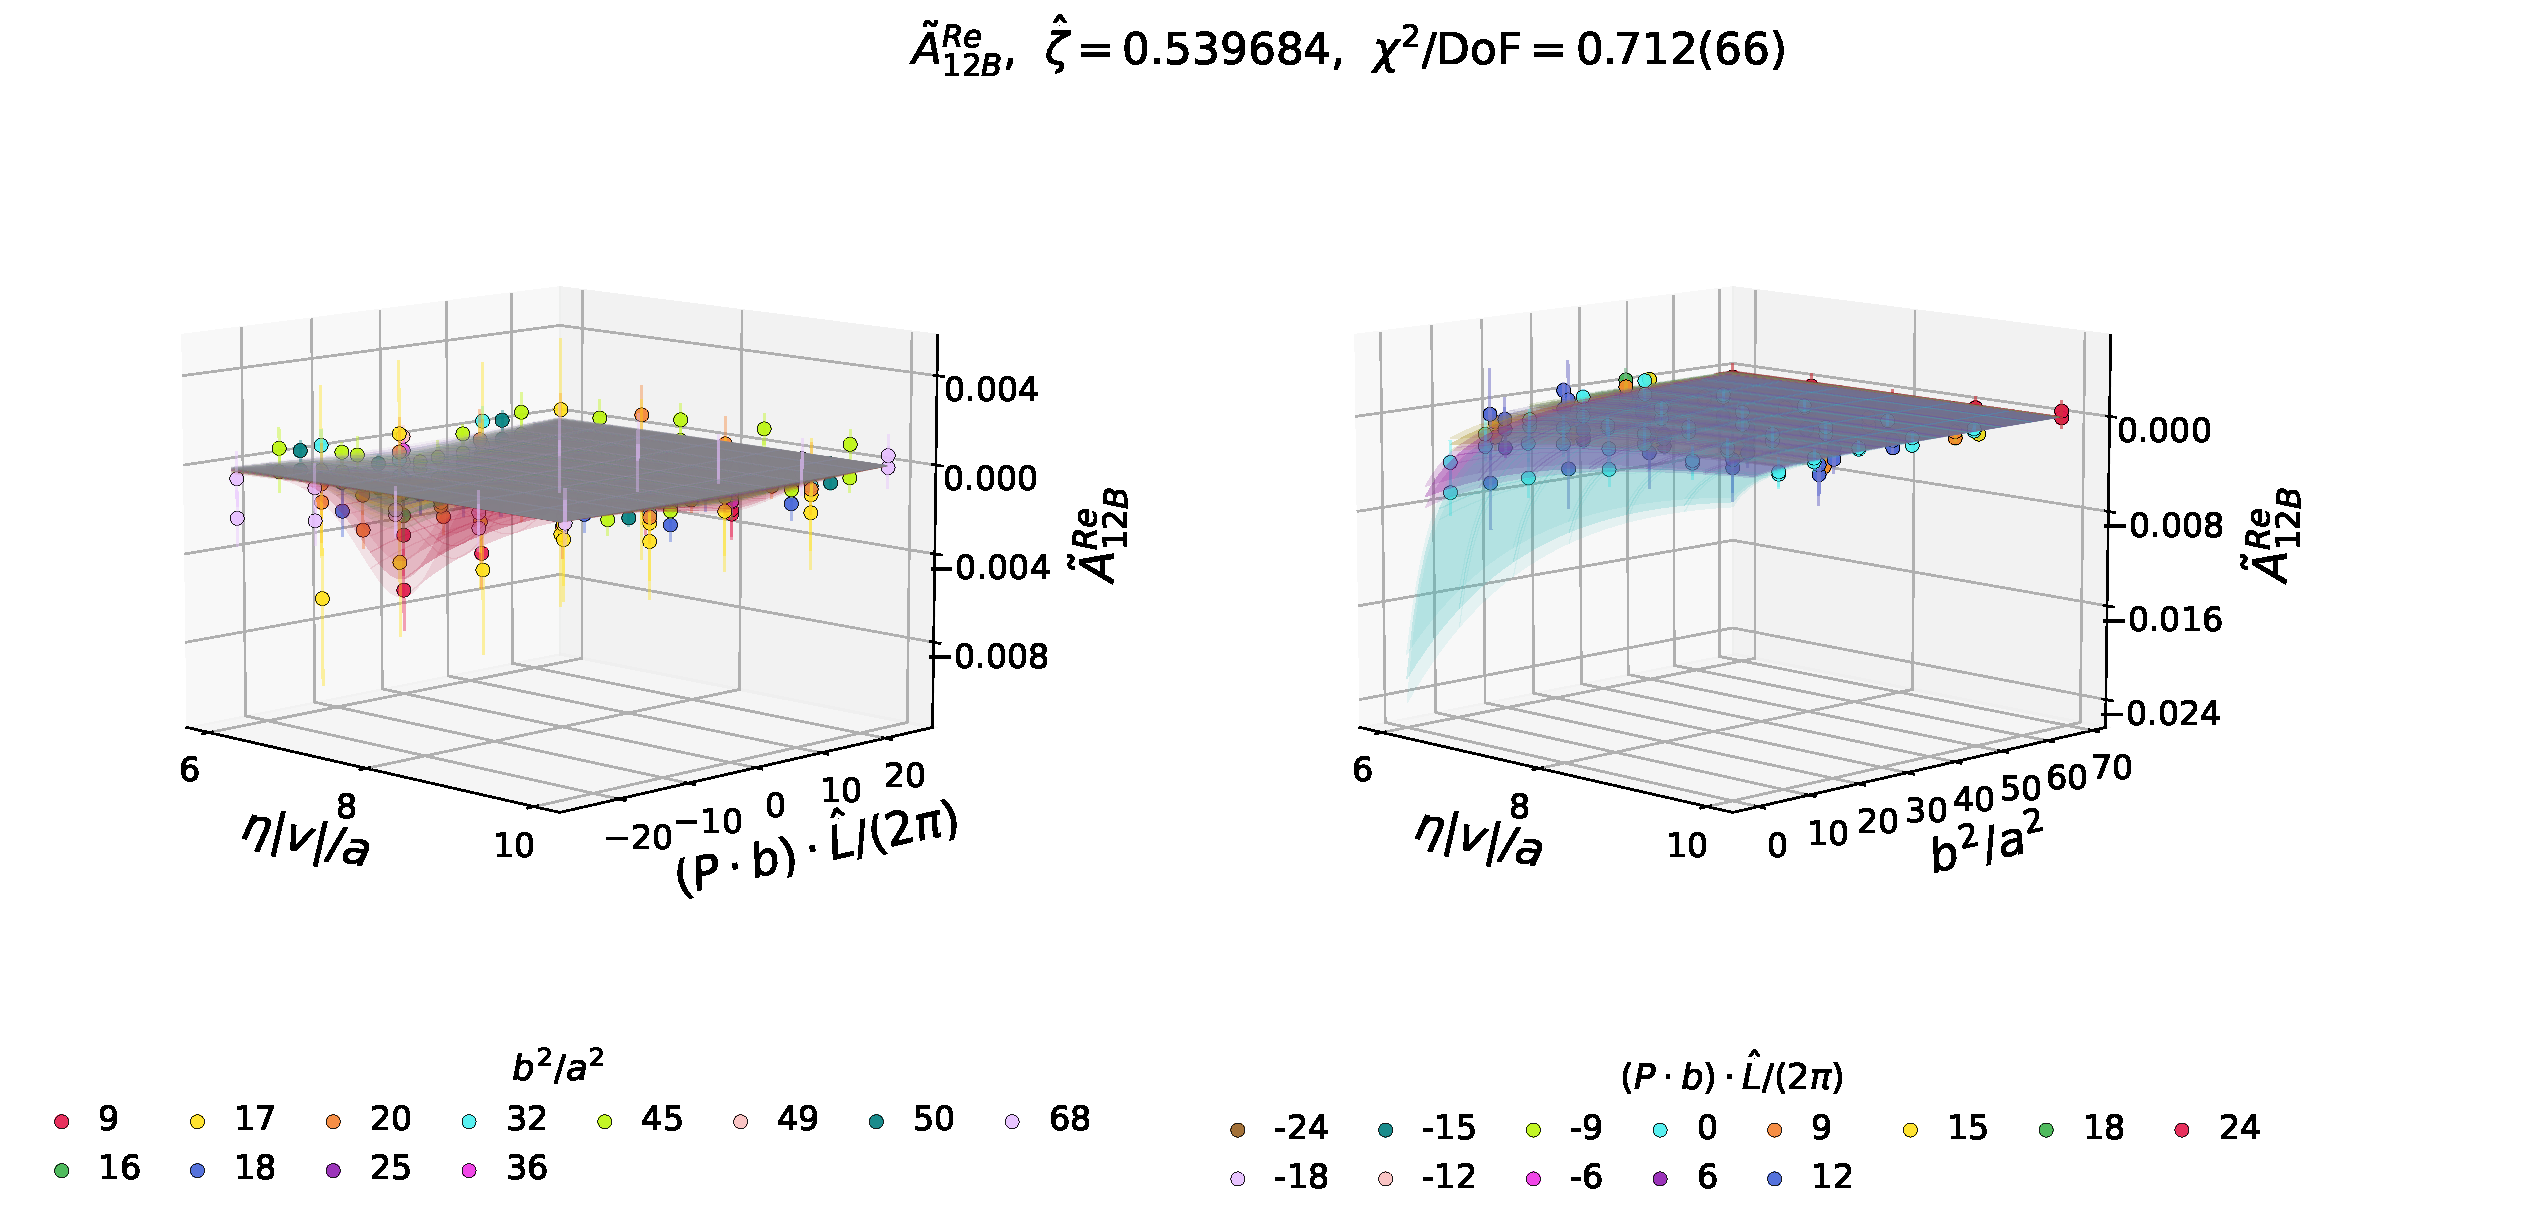
\includegraphics[width=\linewidth,height=.70\textheight,keepaspectratio]{fitting/ReA12B_Pb_bsq_PL-3_WithFit_3D.pdf}
\par\small Invariant coordinates: $(\nu,b^2,\eta)$. All panels and data overlays retained.

\figsrc{Thesis: plots; ReA12B\_Pb\_bsq\_PL-3\_WithFit\_3D}
\end{frame}

\begin{frame}{Fixed staple $\eta=8$: $\tAmp_{12B}^{\mathrm{Re}}$, $P_L=-3$}
\centering
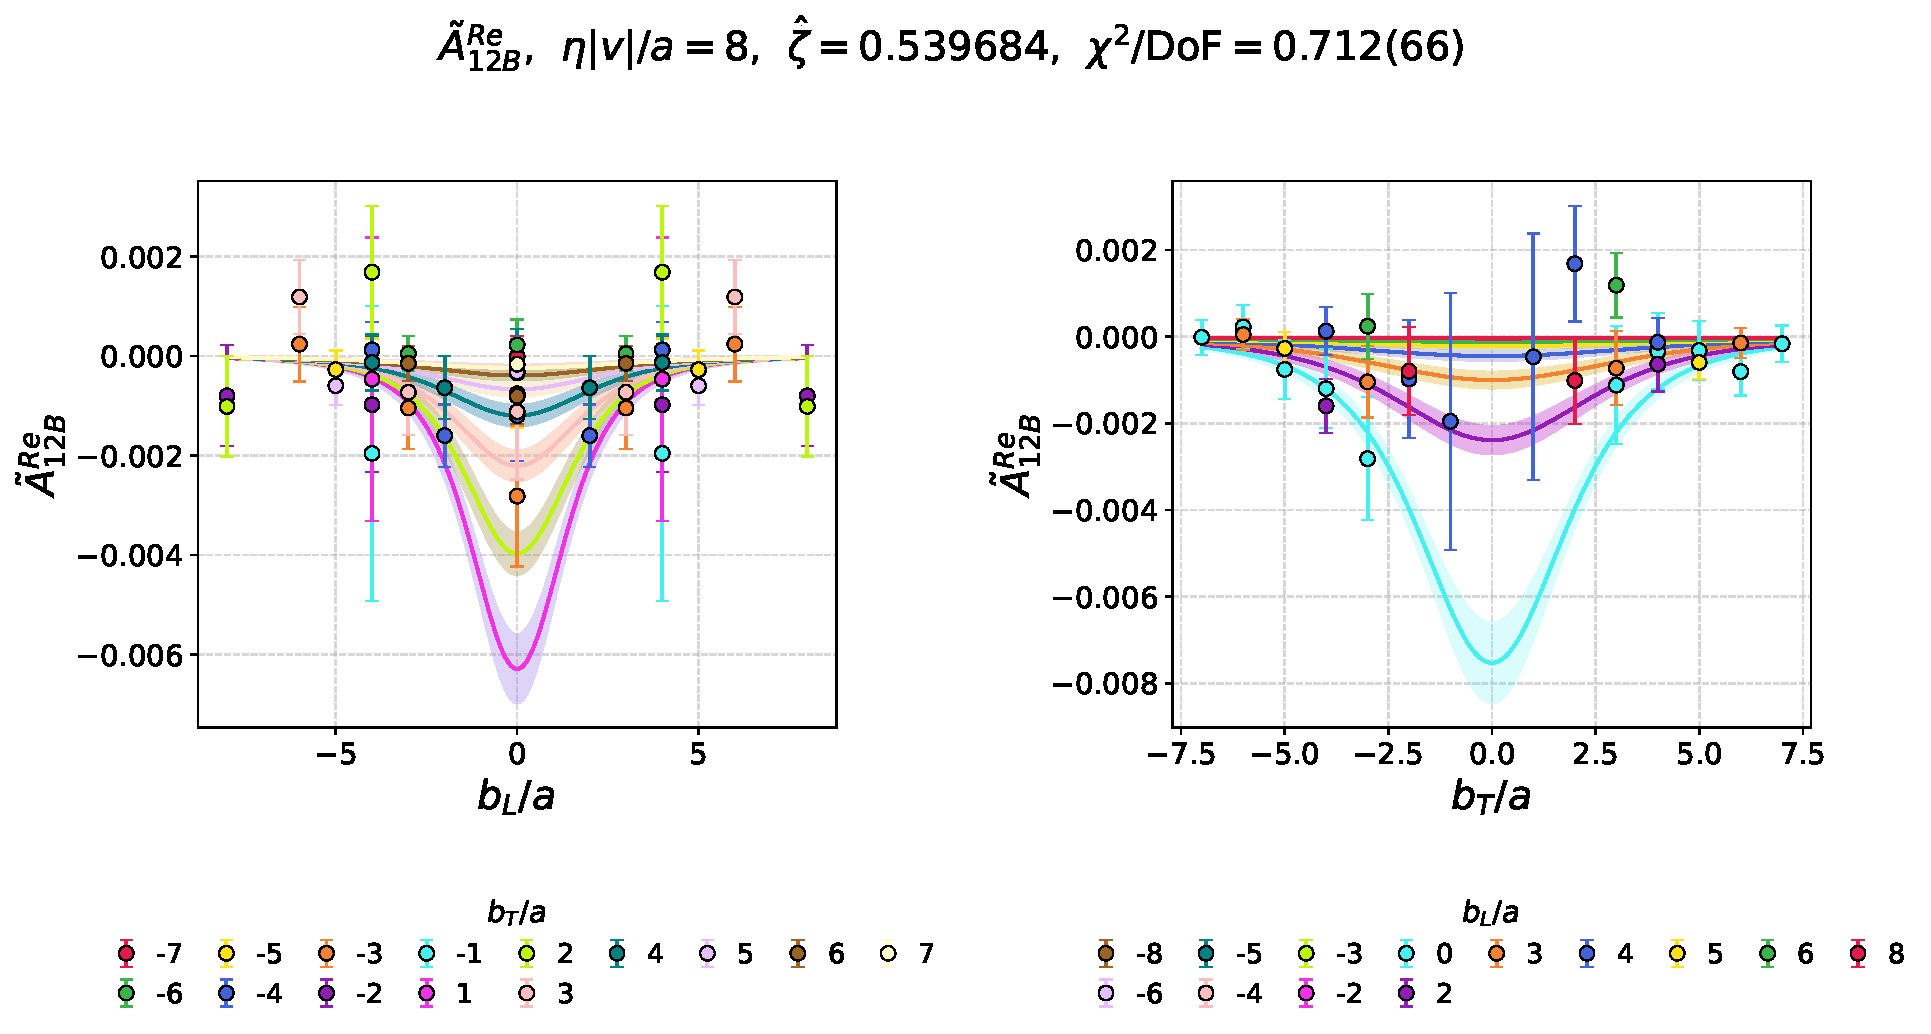
\includegraphics[width=\linewidth,height=.70\textheight,keepaspectratio]{fitting/ReA12B_eta8_PL-3_WithFit_2D.pdf}
\par\small Both spatial-coordinate slices. Same simultaneous fit, with Jackknife bands.

\figsrc{Thesis: plots; ReA12B\_eta8\_PL-3\_WithFit\_2D}
\end{frame}

\begin{frame}{Fixed staple $\eta=8$: $\tAmp_{12B}^{\mathrm{Re}}$, $P_L=-3$}
\centering
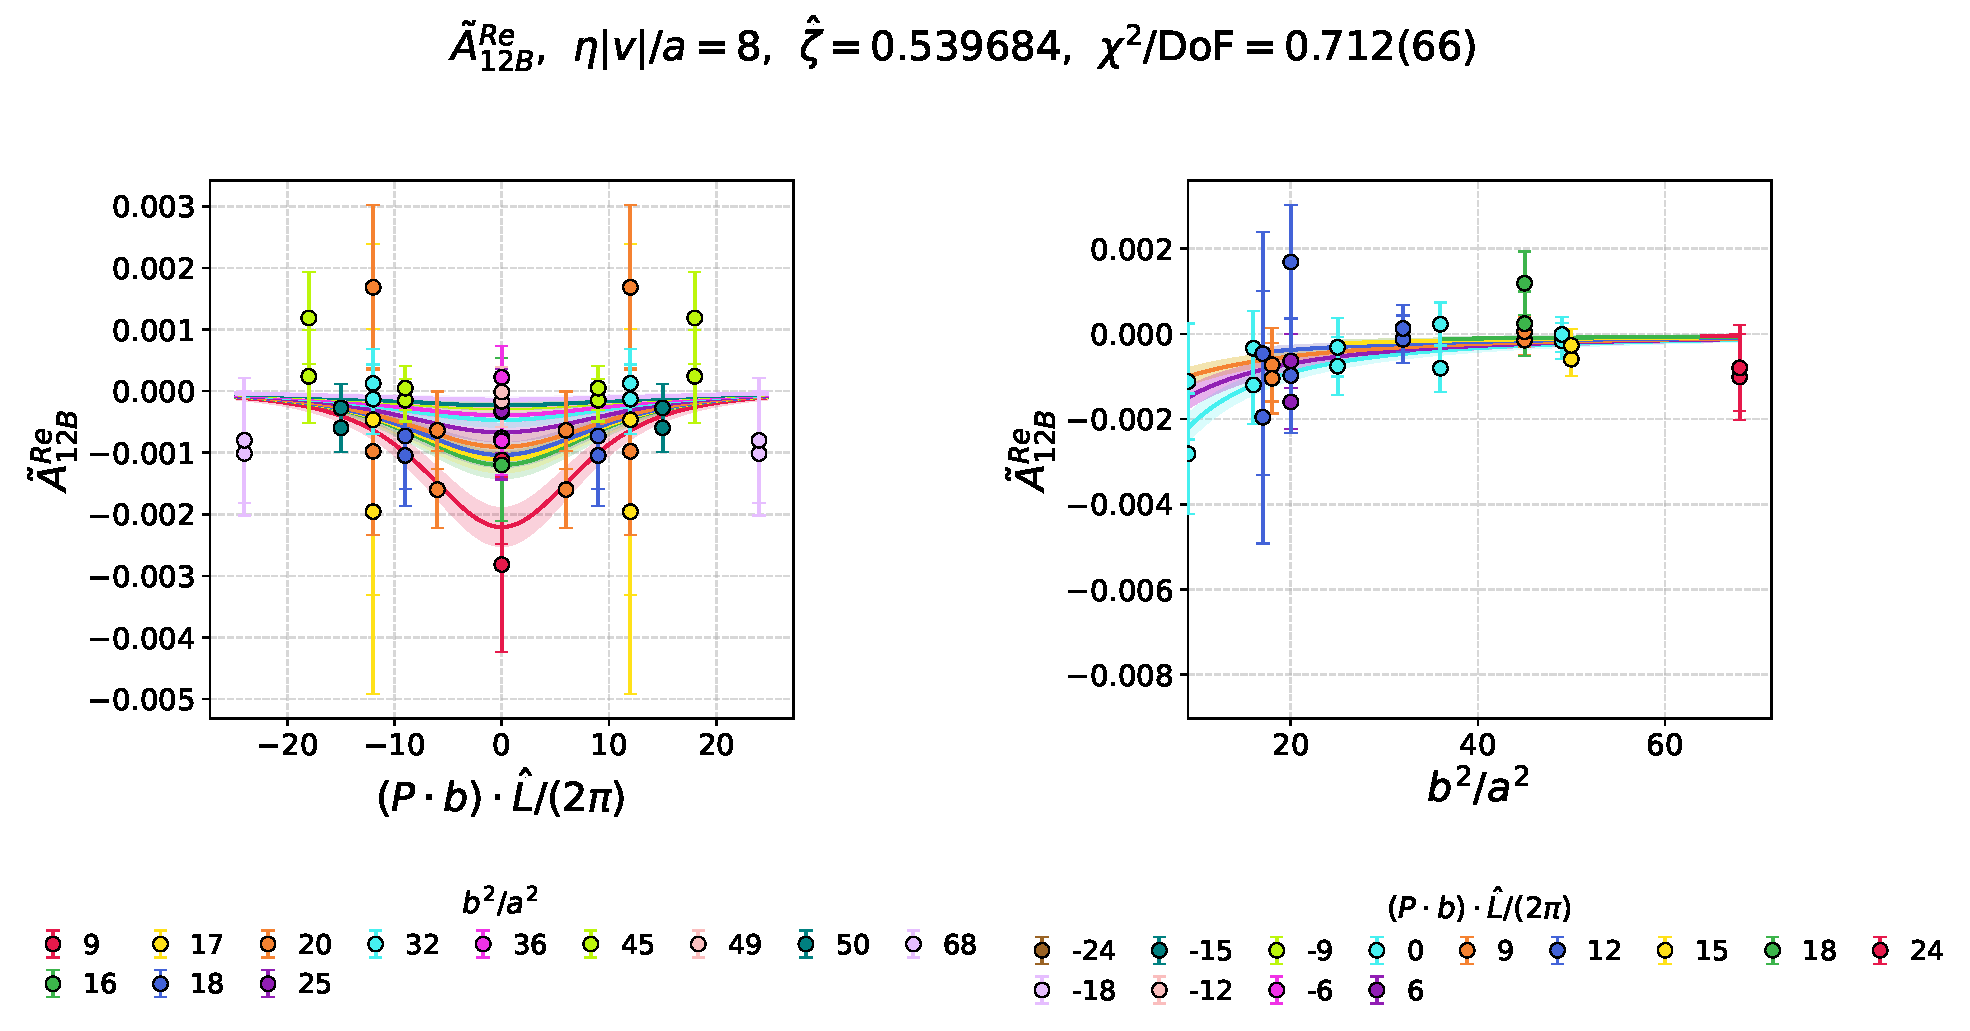
\includegraphics[width=\linewidth,height=.70\textheight,keepaspectratio]{fitting/ReA12B_Pb_bsq_eta8_PL-3_WithFit_2D.pdf}
\par\small Both invariant-coordinate slices. Same simultaneous fit, with Jackknife bands.

\figsrc{Thesis: plots; ReA12B\_Pb\_bsq\_eta8\_PL-3\_WithFit\_2D}
\end{frame}

\begin{frame}{Integrated Fourier results: $P_L=-3$}
\small\renewcommand{\arraystretch}{1.8}\begin{tabular}{lcccc}\toprule Integral & $(-\infty,\infty)$ & $[-1,1]$ & $[-1,0]$ & $[0,1]$\\\midrule
$\int dx\,E$ & 0.759(69) & 0.754(70) & 0.377(35) & 0.377(35) \\
$\int dx\,O$ & -1(320)e-17 & 2(33)e-16 & 0.234(23) & -0.235(23) \\
$\int dx\,\tilde f_1^{(0)}$ & 1.52(14) & 1.51(14) & 0.286(55) & 1.22(11) \\
$\int dx\,\tilde f_{1T}^{\perp(1)}$ & 0.333(51) & 0.333(51) & 0.167(25) & 0.167(25) \\
$m_N\int dx\,\tilde f_{1T}^{\perp(1)}/\int dx\,\tilde f_1^{(0)}$ & 0.236(32) & 0.238(32) & 0.63(13) & 0.147(20) \\
\bottomrule\end{tabular}\par\medskip $b^2=9a^2$; all values and Jackknife uncertainties retained. Numerical values retain the source normalization. The last row is in GeV.
\figsrc{Thesis: SimultaneousFitsCov/Integration\_Table\_PL-3\_bmin3\_b2-9.tex}
\end{frame}

\begin{frame}{Fourier results (2D): $P_L=-3$, unpolarized}
\centering
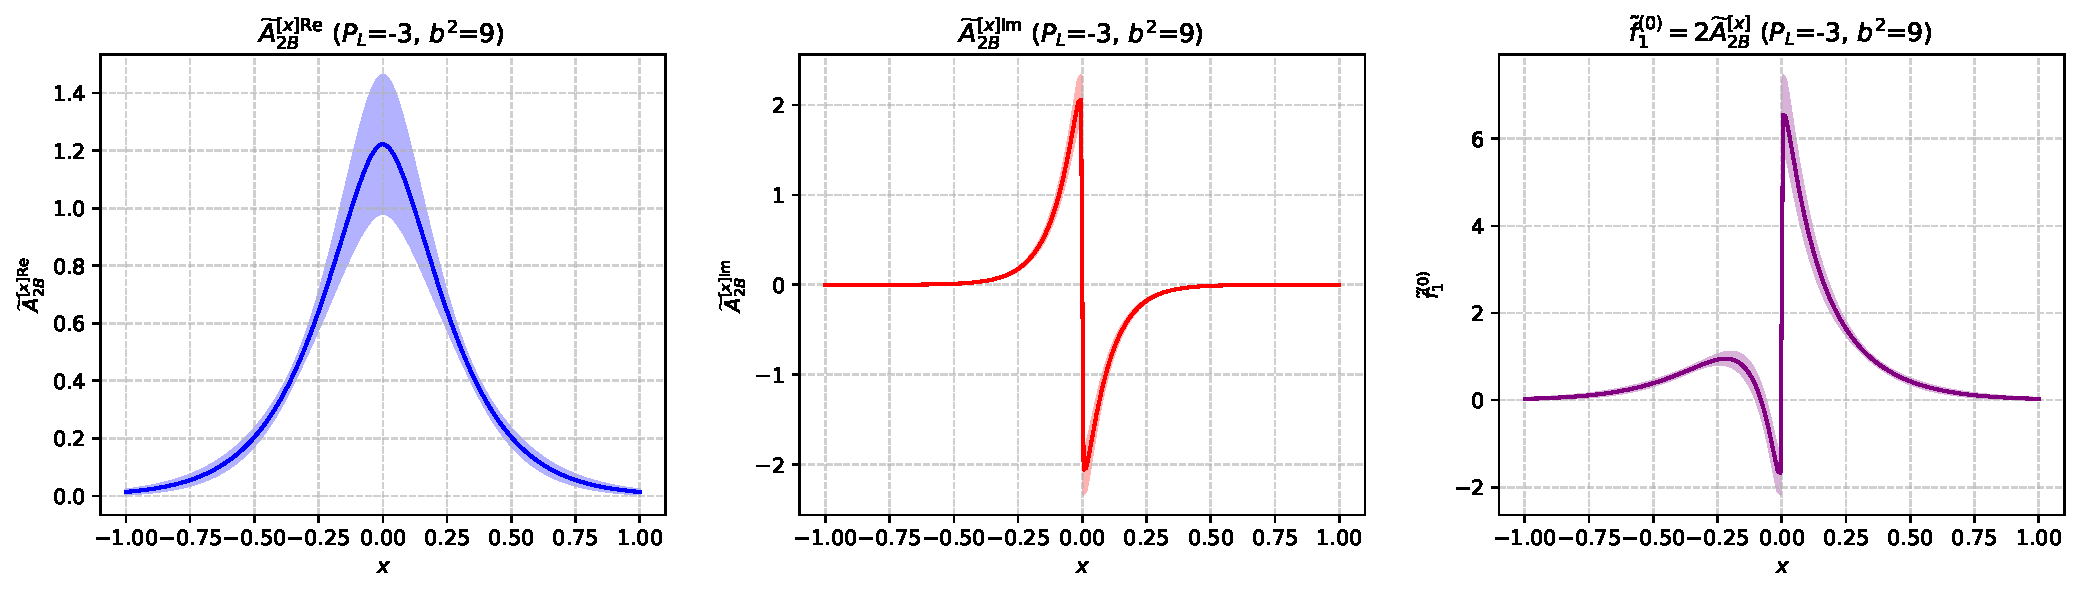
\includegraphics[width=\linewidth,height=.70\textheight,keepaspectratio]{fitting/FT_xdep_A2B_A12B_bmin3_eta610_b2-9_PL-3__row1.pdf}
\par\small Even, odd, and unpolarized transforms. Fixed $b^2=9a^2$.

\figsrc{Thesis: SimultaneousFitsCov; FT\_xdep\_A2B\_A12B\_bmin3\_eta610\_b2-9\_PL-3}
\end{frame}

\begin{frame}{Fourier results (2D): $P_L=-3$, Sivers}
\centering
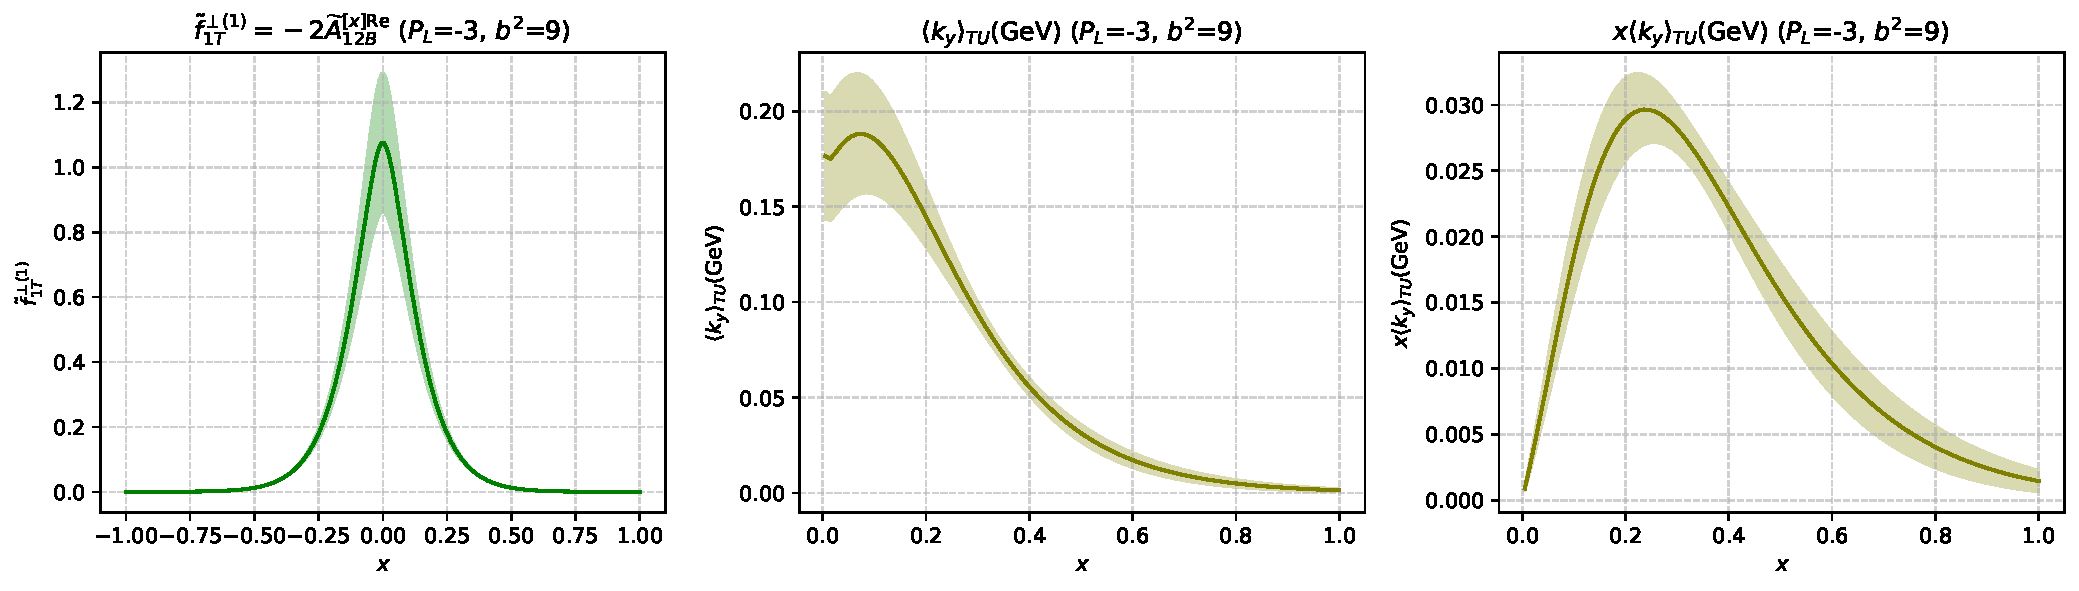
\includegraphics[width=\linewidth,height=.70\textheight,keepaspectratio]{fitting/FT_xdep_A2B_A12B_bmin3_eta610_b2-9_PL-3__row2.pdf}
\par\small Sivers transform, shift, and $x\langle k_y\rangle_{TU}$. Fixed $b^2=9a^2$.

\figsrc{Thesis: SimultaneousFitsCov; FT\_xdep\_A2B\_A12B\_bmin3\_eta610\_b2-9\_PL-3}
\end{frame}

\begin{frame}{Fourier results (3D): $P_L=-3$, unpolarized}
\centering
\includegraphics[width=\linewidth,height=.70\textheight,keepaspectratio]{fitting/FT_xdep_3D_A2B_A12B_bmin3_eta610_PL-3__row1.pdf}
\par\small Even, odd, and unpolarized transforms. Full $b^2/a^2\in[9,68]$ dependence.

\figsrc{Thesis: SimultaneousFitsCov; FT\_xdep\_3D\_A2B\_A12B\_bmin3\_eta610\_PL-3}
\end{frame}

\begin{frame}{Fourier results (3D): $P_L=-3$, Sivers}
\centering
\includegraphics[width=\linewidth,height=.70\textheight,keepaspectratio]{fitting/FT_xdep_3D_A2B_A12B_bmin3_eta610_PL-3__row2.pdf}
\par\small Sivers transform, shift, and $x\langle k_y\rangle_{TU}$. Full $b^2/a^2\in[9,68]$ dependence.

\figsrc{Thesis: SimultaneousFitsCov; FT\_xdep\_3D\_A2B\_A12B\_bmin3\_eta610\_PL-3}
\end{frame}

\begin{frame}{Simultaneous fit parameters: $P_L=-4$}
\small $|\vect b|\ge3a$, $6\le\eta\le10$; reported $\chi^2_{\rm aug}/N_{\rm data}=0.434(51)$.\par\medskip
\begin{columns}[t]\begin{column}{.32\textwidth}\centering $\tAmp_{2B}^{\mathrm{Re}}$\par\medskip\renewcommand{\arraystretch}{1.3}\begin{tabular}{cc}\toprule Parameter & Value\\\midrule
$a$ & $4.0086(15)$ \\
$c$ & $0.27(21)$ \\
$d$ & $0.122(13)$ \\
$k_1$ & $12.2751(58)$ \\
$k_2$ & $-36.19925(89)$ \\
$j$ & $2.0654(56)$ \\
$f$ & $0.577(19)$ \\\bottomrule\end{tabular}\end{column}\begin{column}{.32\textwidth}\centering $\tAmp_{2B}^{\mathrm{Im}}$\par\medskip\renewcommand{\arraystretch}{1.3}\begin{tabular}{cc}\toprule Parameter & Value\\\midrule
$a''$ & $0.269(13)$ \\
$c''$ & $0.264(47)$ \\
$d''$ & $0.196(14)$ \\
$j''$ & $1.0084(79)$ \\
$f$ & $0.577(19)$ \\\bottomrule\end{tabular}\end{column}\begin{column}{.32\textwidth}\centering $\tAmp_{12B}^{\mathrm{Re}}$\par\medskip\renewcommand{\arraystretch}{1.3}\begin{tabular}{cc}\toprule Parameter & Value\\\midrule
$a'$ & $0.5824(55)$ \\
$c'$ & $0.116(19)$ \\
$d'$ & $0.102(18)$ \\
$j'$ & $2.0059(34)$ \\
$f$ & $0.577(19)$ \\\bottomrule\end{tabular}\end{column}\end{columns}
\figsrc{Thesis: SimultaneousFitsCov/Fit\_Table\_PL-4\_bmin3.tex}
\end{frame}

\begin{frame}{Global fit: $\tAmp_{2B}^{\mathrm{Re}}$, $P_L=-4$}
\centering
\includegraphics[width=\linewidth,height=.70\textheight,keepaspectratio]{fitting/ReA2B_PL-4_WithFit_3D.pdf}
\par\small Spatial coordinates: $(b_L,b_T,\eta)$. All panels and data overlays retained.

\figsrc{Thesis: plots; ReA2B\_PL-4\_WithFit\_3D}
\end{frame}

\begin{frame}{Global fit: $\tAmp_{2B}^{\mathrm{Re}}$, $P_L=-4$}
\centering
\includegraphics[width=\linewidth,height=.70\textheight,keepaspectratio]{fitting/ReA2B_Pb_bsq_PL-4_WithFit_3D.pdf}
\par\small Invariant coordinates: $(\nu,b^2,\eta)$. All panels and data overlays retained.

\figsrc{Thesis: plots; ReA2B\_Pb\_bsq\_PL-4\_WithFit\_3D}
\end{frame}

\begin{frame}{Fixed staple $\eta=8$: $\tAmp_{2B}^{\mathrm{Re}}$, $P_L=-4$}
\centering
\includegraphics[width=\linewidth,height=.70\textheight,keepaspectratio]{fitting/ReA2B_eta8_PL-4_WithFit_2D.pdf}
\par\small Both spatial-coordinate slices. Same simultaneous fit, with Jackknife bands.

\figsrc{Thesis: plots; ReA2B\_eta8\_PL-4\_WithFit\_2D}
\end{frame}

\begin{frame}{Fixed staple $\eta=8$: $\tAmp_{2B}^{\mathrm{Re}}$, $P_L=-4$}
\centering
\includegraphics[width=\linewidth,height=.70\textheight,keepaspectratio]{fitting/ReA2B_Pb_bsq_eta8_PL-4_WithFit_2D.pdf}
\par\small Both invariant-coordinate slices. Same simultaneous fit, with Jackknife bands.

\figsrc{Thesis: plots; ReA2B\_Pb\_bsq\_eta8\_PL-4\_WithFit\_2D}
\end{frame}

\begin{frame}{Global fit: $\tAmp_{2B}^{\mathrm{Im}}$, $P_L=-4$}
\centering
\includegraphics[width=\linewidth,height=.70\textheight,keepaspectratio]{fitting/ImA2B_PL-4_WithFit_3D.pdf}
\par\small Spatial coordinates: $(b_L,b_T,\eta)$. All panels and data overlays retained.

\figsrc{Thesis: plots; ImA2B\_PL-4\_WithFit\_3D}
\end{frame}

\begin{frame}{Global fit: $\tAmp_{2B}^{\mathrm{Im}}$, $P_L=-4$}
\centering
\includegraphics[width=\linewidth,height=.70\textheight,keepaspectratio]{fitting/ImA2B_Pb_bsq_PL-4_WithFit_3D.pdf}
\par\small Invariant coordinates: $(\nu,b^2,\eta)$. All panels and data overlays retained.

\figsrc{Thesis: plots; ImA2B\_Pb\_bsq\_PL-4\_WithFit\_3D}
\end{frame}

\begin{frame}{Fixed staple $\eta=8$: $\tAmp_{2B}^{\mathrm{Im}}$, $P_L=-4$}
\centering
\includegraphics[width=\linewidth,height=.70\textheight,keepaspectratio]{fitting/ImA2B_eta8_PL-4_WithFit_2D.pdf}
\par\small Both spatial-coordinate slices. Same simultaneous fit, with Jackknife bands.

\figsrc{Thesis: plots; ImA2B\_eta8\_PL-4\_WithFit\_2D}
\end{frame}

\begin{frame}{Fixed staple $\eta=8$: $\tAmp_{2B}^{\mathrm{Im}}$, $P_L=-4$}
\centering
\includegraphics[width=\linewidth,height=.70\textheight,keepaspectratio]{fitting/ImA2B_Pb_bsq_eta8_PL-4_WithFit_2D.pdf}
\par\small Both invariant-coordinate slices. Same simultaneous fit, with Jackknife bands.

\figsrc{Thesis: plots; ImA2B\_Pb\_bsq\_eta8\_PL-4\_WithFit\_2D}
\end{frame}

\begin{frame}{Global fit: $\tAmp_{12B}^{\mathrm{Re}}$, $P_L=-4$}
\centering
\includegraphics[width=\linewidth,height=.70\textheight,keepaspectratio]{fitting/ReA12B_PL-4_WithFit_3D.pdf}
\par\small Spatial coordinates: $(b_L,b_T,\eta)$. All panels and data overlays retained.

\figsrc{Thesis: plots; ReA12B\_PL-4\_WithFit\_3D}
\end{frame}

\begin{frame}{Global fit: $\tAmp_{12B}^{\mathrm{Re}}$, $P_L=-4$}
\centering
\includegraphics[width=\linewidth,height=.70\textheight,keepaspectratio]{fitting/ReA12B_Pb_bsq_PL-4_WithFit_3D.pdf}
\par\small Invariant coordinates: $(\nu,b^2,\eta)$. All panels and data overlays retained.

\figsrc{Thesis: plots; ReA12B\_Pb\_bsq\_PL-4\_WithFit\_3D}
\end{frame}

\begin{frame}{Fixed staple $\eta=8$: $\tAmp_{12B}^{\mathrm{Re}}$, $P_L=-4$}
\centering
\includegraphics[width=\linewidth,height=.70\textheight,keepaspectratio]{fitting/ReA12B_eta8_PL-4_WithFit_2D.pdf}
\par\small Both spatial-coordinate slices. Same simultaneous fit, with Jackknife bands.

\figsrc{Thesis: plots; ReA12B\_eta8\_PL-4\_WithFit\_2D}
\end{frame}

\begin{frame}{Fixed staple $\eta=8$: $\tAmp_{12B}^{\mathrm{Re}}$, $P_L=-4$}
\centering
\includegraphics[width=\linewidth,height=.70\textheight,keepaspectratio]{fitting/ReA12B_Pb_bsq_eta8_PL-4_WithFit_2D.pdf}
\par\small Both invariant-coordinate slices. Same simultaneous fit, with Jackknife bands.

\figsrc{Thesis: plots; ReA12B\_Pb\_bsq\_eta8\_PL-4\_WithFit\_2D}
\end{frame}

\begin{frame}{Integrated Fourier results: $P_L=-4$}
\small\renewcommand{\arraystretch}{1.8}\begin{tabular}{lcccc}\toprule Integral & $(-\infty,\infty)$ & $[-1,1]$ & $[-1,0]$ & $[0,1]$\\\midrule
$\int dx\,E$ & 0.87(10) & 0.87(10) & 0.434(52) & 0.434(52) \\
$\int dx\,O$ & 3(207)e-17 & 2(21)e-16 & 0.153(26) & -0.154(26) \\
$\int dx\,\tilde f_1^{(0)}$ & 1.74(21) & 1.74(21) & 0.56(12) & 1.18(12) \\
$\int dx\,\tilde f_{1T}^{\perp(1)}$ & 0.315(55) & 0.315(55) & 0.157(28) & 0.157(28) \\
$m_N\int dx\,\tilde f_{1T}^{\perp(1)}/\int dx\,\tilde f_1^{(0)}$ & 0.195(37) & 0.195(37) & 0.301(73) & 0.144(27) \\
\bottomrule\end{tabular}\par\medskip $b^2=9a^2$; all values and Jackknife uncertainties retained. Numerical values retain the source normalization. The last row is in GeV.
\figsrc{Thesis: SimultaneousFitsCov/Integration\_Table\_PL-4\_bmin3\_b2-9.tex}
\end{frame}

\begin{frame}{Fourier results (2D): $P_L=-4$, unpolarized}
\centering
\includegraphics[width=\linewidth,height=.70\textheight,keepaspectratio]{fitting/FT_xdep_A2B_A12B_bmin3_eta610_b2-9_PL-4__row1.pdf}
\par\small Even, odd, and unpolarized transforms. Fixed $b^2=9a^2$.

\figsrc{Thesis: SimultaneousFitsCov; FT\_xdep\_A2B\_A12B\_bmin3\_eta610\_b2-9\_PL-4}
\end{frame}

\begin{frame}{Fourier results (2D): $P_L=-4$, Sivers}
\centering
\includegraphics[width=\linewidth,height=.70\textheight,keepaspectratio]{fitting/FT_xdep_A2B_A12B_bmin3_eta610_b2-9_PL-4__row2.pdf}
\par\small Sivers transform, shift, and $x\langle k_y\rangle_{TU}$. Fixed $b^2=9a^2$.

\figsrc{Thesis: SimultaneousFitsCov; FT\_xdep\_A2B\_A12B\_bmin3\_eta610\_b2-9\_PL-4}
\end{frame}

\begin{frame}{Fourier results (3D): $P_L=-4$, unpolarized}
\centering
\includegraphics[width=\linewidth,height=.70\textheight,keepaspectratio]{fitting/FT_xdep_3D_A2B_A12B_bmin3_eta610_PL-4__row1.pdf}
\par\small Even, odd, and unpolarized transforms. Full $b^2/a^2\in[9,68]$ dependence.

\figsrc{Thesis: SimultaneousFitsCov; FT\_xdep\_3D\_A2B\_A12B\_bmin3\_eta610\_PL-4}
\end{frame}

\begin{frame}{Fourier results (3D): $P_L=-4$, Sivers}
\centering
\includegraphics[width=\linewidth,height=.70\textheight,keepaspectratio]{fitting/FT_xdep_3D_A2B_A12B_bmin3_eta610_PL-4__row2.pdf}
\par\small Sivers transform, shift, and $x\langle k_y\rangle_{TU}$. Full $b^2/a^2\in[9,68]$ dependence.

\figsrc{Thesis: SimultaneousFitsCov; FT\_xdep\_3D\_A2B\_A12B\_bmin3\_eta610\_PL-4}
\end{frame}

\begin{frame}{Separable simultaneous candidate: ExpPb / Expb}
\begin{align*}
\tAmp_{2B}^{\mathrm{Re}}&=a_Re^{-c_R|\nu|}e^{-d_R\sqrt{b^2}}e^{-f\eta}\\[4mm]
\tAmp_{2B}^{\mathrm{Im}}&=a_I\nu e^{-c_I|\nu|}e^{-d_I\sqrt{b^2}}e^{-f\eta}\\[4mm]
\tAmp_{12B}^{\mathrm{Re}}&=-a_Se^{-c_S|\nu|}e^{-d_S\sqrt{b^2}}e^{-f\eta}\\[4mm]
\end{align*} Shared $f$; the spatial coefficients are fitted separately for $R,I,S$. All fits retain the same cut and staple interval.
\figsrc{Thesis: Fitting Methodologies and Stability Analysis}
\end{frame}

\begin{frame}{Separable simultaneous candidate: ExpPb / PowerLawb}
\begin{align*}
\tAmp_{2B}^{\mathrm{Re}}&=a_Re^{-c_R|\nu|}(1+d_Rb^2)^{-j_R}e^{-f\eta}\\[4mm]
\tAmp_{2B}^{\mathrm{Im}}&=a_I\nu e^{-c_I|\nu|}(1+d_Ib^2)^{-j_I}e^{-f\eta}\\[4mm]
\tAmp_{12B}^{\mathrm{Re}}&=-a_Se^{-c_S|\nu|}(1+d_Sb^2)^{-j_S}e^{-f\eta}\\[4mm]
\end{align*} Shared $f$; the spatial coefficients are fitted separately for $R,I,S$. All fits retain the same cut and staple interval.
\figsrc{Thesis: Fitting Methodologies and Stability Analysis}
\end{frame}

\begin{frame}{Separable simultaneous candidate: GaussianPb / Expb}
\begin{align*}
\tAmp_{2B}^{\mathrm{Re}}&=a_Re^{-c_R\nu^2}e^{-d_R\sqrt{b^2}}e^{-f\eta}\\[4mm]
\tAmp_{2B}^{\mathrm{Im}}&=a_I\nu e^{-c_I\nu^2}e^{-d_I\sqrt{b^2}}e^{-f\eta}\\[4mm]
\tAmp_{12B}^{\mathrm{Re}}&=-a_Se^{-c_S\nu^2}e^{-d_S\sqrt{b^2}}e^{-f\eta}\\[4mm]
\end{align*} Shared $f$; the spatial coefficients are fitted separately for $R,I,S$. All fits retain the same cut and staple interval.
\figsrc{Thesis: Fitting Methodologies and Stability Analysis}
\end{frame}

\begin{frame}{Separable simultaneous candidate: GaussianPb / PowerLawb}
\begin{align*}
\tAmp_{2B}^{\mathrm{Re}}&=a_Re^{-c_R\nu^2}(1+d_Rb^2)^{-j_R}e^{-f\eta}\\[4mm]
\tAmp_{2B}^{\mathrm{Im}}&=a_I\nu e^{-c_I\nu^2}(1+d_Ib^2)^{-j_I}e^{-f\eta}\\[4mm]
\tAmp_{12B}^{\mathrm{Re}}&=-a_Se^{-c_S\nu^2}(1+d_Sb^2)^{-j_S}e^{-f\eta}\\[4mm]
\end{align*} Shared $f$; the spatial coefficients are fitted separately for $R,I,S$. All fits retain the same cut and staple interval.
\figsrc{Thesis: Fitting Methodologies and Stability Analysis}
\end{frame}

\begin{frame}{Separable candidates: fit quality at every momentum}

\small\renewcommand{\arraystretch}{1.6}\begin{tabular}{lcccc}\toprule
Model & $P_L=-1$ & $P_L=-2$ & $P_L=-3$ & $P_L=-4$\\\midrule
ExpPb / Expb & $1.406(92)$ & $0.956(75)$ & $0.622(61)$ & $0.455(53)$\\
ExpPb / PowerLawb & $1.286(89)$ & $0.938(75)$ & $0.623(61)$ & $0.447(53)$\\
GaussianPb / Expb & $2.389(121)$ & $2.005(111)$ & $0.945(76)$ & $0.453(52)$\\
GaussianPb / PowerLawb & $2.316(120)$ & $1.981(111)$ & $0.948(76)$ & $0.448(52)$\\
Coupled power law & $1.85(10)$ & $1.197(85)$ & $0.712(66)$ & $0.434(51)$\\\bottomrule
\end{tabular}\par\medskip Entries reproduce the thesis-reported $\chi^2/\mathrm{dof}$. The coupled fit uses the augmented objective with priors; raw values alone do not establish a model preference.
\figsrc{Thesis: Fitting Methodologies and Stability Analysis}
\end{frame}

\begin{frame}{Separable candidates: width and sign diagnostics}

\small\renewcommand{\arraystretch}{1.5}\begin{tabular}{lccc}\toprule
Model at $P_L=-1$ & $c_I$ & $c_S$ & $a_I$\\\midrule
ExpPb / Expb & $0.0010(262)$ & $0.045(23)$ & $-0.167(16)$\\
ExpPb / PowerLawb & $0.0045(248)$ & $0.028(24)$ & $-0.167(31)$\\
GaussianPb / Expb & $0.568(171)$ & $0.0038(69)$ & $+0.050(121)$\\
GaussianPb / PowerLawb & $0.602(48)$ & $0.0016(61)$ & $+0.168(92)$\\
Coupled power law & $0.2253(69)$ & $0.0773(46)$ & $+0.267(13)$\\\bottomrule
\end{tabular}
\begin{itemize}
\item Several separable widths are statistically compatible with zero: longitudinal decay is weakly constrained. At $c=0$ it is lost; at $c<0$ the continuation grows.
\item Negative fitted $a_I$ is a sign mismatch with the selected convention, not a general prohibition on signed amplitudes.
\item For $c>0$, $e^{-c|\nu|}$ has a first-derivative cusp; $\nu e^{-c|\nu|}$ has a continuous first derivative but a discontinuous second derivative. Odd parity alone does not exclude it.
\end{itemize}
\figsrc{Thesis: Fitting Methodologies and Stability Analysis}
\end{frame}

\begin{frame}{What survives the complete model comparison}

\begin{itemize}
\item The chosen power law couples $\nu^2$ and $b^2$ in one denominator and supports the required Fourier continuation under explicit positivity and exponent conditions.
\item The three-amplitude fit, not the real unpolarized channel alone, constrains the Sivers shift.
\item All four momenta have now been inspected in spatial coordinates, invariant coordinates, $x$ space, and integrated observables.
\item The next step extrapolates the resulting shift in $\hat\zeta$ while carrying the model and statistical limitations forward.
\end{itemize}
\figsrc{Thesis: Fitting Methodologies and Stability Analysis}
\end{frame}

% ===================== Extrapolations to the physical limit (thesis Ch. 7) =====================
\section{Extrapolations to the physical limit}

\begin{frame}{Extrapolations to the physical limit}
  \begin{columns}[c]
    \begin{column}{0.46\textwidth}\centering
      \includegraphics[width=\linewidth,height=0.6\textheight,keepaspectratio]{SimulFit_Distinct_1_over_PL_bmin3_eta610_b29.0_Amps.pdf}
    \end{column}
    \begin{column}{0.52\textwidth}\centering
      \includegraphics[width=\linewidth,height=0.6\textheight,keepaspectratio]{SimulFit_Distinct_1_over_PL_bmin3_eta610_b29.0_Sivers.pdf}
    \end{column}
  \end{columns}
  {\scriptsize Left: discrete $\hat\zeta$ slices of $\tAmp^{[x]\text{Re}}_{2B}$, $\tAmp^{[x]\text{Im}}_{2B}$, $\tilde f_1^{(0)}=2\tAmp^{[x]}_{2B}$ and $\tilde f_{1T}^{\perp(1)}=-2\tAmp^{[x]\text{Re}}_{12B}$ against $x$ and $1/\hat\zeta$ at $|b_T|=3a\approx0.34$ fm; one ribbon per momentum $P_L=-1,\dots,-4$ ($1/\hat\zeta=11.02,3.40,1.85,1.27$). The drift with $1/\hat\zeta$ motivates the extrapolation $\hat\zeta\to\infty$.
  Right: Sivers shift $\langle k_y\rangle_{TU}$ and $x\langle k_y\rangle_{TU}$ for the same momenta and $|b_T|$, restricted to $x\ge0$.}
\end{frame}

\begin{frame}{Extrapolation $\zetahat\to\infty$}
  \centering
  \includegraphics[height=0.68\textheight]{Param_Extrapolations_1byZetahat_sq_P234_bmin3_eta610_b29.0.pdf}\\
  {\scriptsize Twelve simultaneous-fit parameters vs $1/\hat\zeta$, using only $P_L=-2,-3,-4$ (black points). Dashed red curve and band: fitted ansatz $c+d/\hat\zeta^2$, with each panel's Jackknife $\chi^2/\mathrm{dof}$ in its title; blue square at $1/\hat\zeta=0$: extrapolated value. $c_{\rm re}$, $c_{\rm im}$ and $c_{\rm re}^{A_{12B}}$ are rescaled by $1/P_L^2$, $a_{\rm im}$ by $1/P_L$.}
\end{frame}

\begin{frame}{Amplitudes reconstructed at $\zetahat\to\infty$}
  \centering
  \includegraphics[height=0.68\textheight]{Extrapolated_AmpLevel_P234_Sivers_1_over_zetahat_sq_bmin3_eta610_b29.0_Amps.pdf}\\
  {\scriptsize $\tAmp^{[x]\text{Re}}_{2B}$, $\tAmp^{[x]\text{Im}}_{2B}$, $\tilde f_1^{(0)}=2\tAmp^{[x]}_{2B}$ and $\tilde f_{1T}^{\perp(1)}=-2\tAmp^{[x]\text{Re}}_{12B}$ from the extrapolated parameters, as continuous functions of $x$ at $|b_T|=3a\approx0.34$ fm. Bands: Jackknife uncertainty propagated from the twelve parameters.}
\end{frame}

\begin{frame}{Isovector ($u-d$) Sivers shift at $\zetahat\to\infty$}
  \centering
  \includegraphics[width=\linewidth,height=0.6\textheight,keepaspectratio]{Extrapolated_AmpLevel_P234_Sivers_1_over_zetahat_sq_bmin3_eta610_b29.0_Sivers.pdf}\\
  {\scriptsize $\langle k_y\rangle_{TU}$ and $x\langle k_y\rangle_{TU}$ built from the extrapolated amplitudes of the previous slide, restricted to the quark region $x\ge0$. Bands: Jackknife uncertainty.}
\end{frame}

\begin{frame}{Numerical integration of the Fourier transforms at $\zetahat\to\infty$}
  \centering
  \renewcommand{\arraystretch}{1.8}
  \resizebox{\linewidth}{!}{\begin{tabular}{|l|c|c|c|c|}
  \hline
  Integral & $[-\infty, \infty]$ & $[-1, 1]$ & $[-1, 0]$ & $[0, 1]$ \\
  \hline
  $\int dx\, \tAmp^{[x]\text{Re}}_{2B}$ & $0.751(79)$ & $0.751(80)$ & $0.375(40)$ & $0.375(40)$ \\
  $\int dx\, (\tAmp^{[x]\text{Im}}_{2B})$ & $6(96)\times10^{-17}$ & $3(24)\times10^{-16}$ & $0.165(27)$ & $-0.169(29)$ \\
  $\int dx\, \tilde{f}_1^{(0)} = 2\int dx\, (\tAmp^{[x]\text{Re}}_{2B} - \tAmp^{[x]\text{Im}}_{2B})$ & $1.50(16)$ & $1.50(16)$ & $0.421(81)$ & $1.09(11)$ \\
  $\int dx\, \tilde{f}_{1T}^{\perp(1)} = -2\int dx\, \tAmp^{[x]\text{Re}}_{12B}$ & $0.302(53)$ & $0.302(53)$ & $0.151(27)$ & $0.151(27)$ \\
  $m_N \frac{\int dx\, \tilde{f}_{1T}^{\perp(1)}}{\int dx\, \tilde{f}_1^{(0)}}$ & $0.217(38)$ & $0.217(38)$ & $0.387(89)$ & $0.150(26)$ \\
  \hline
  \end{tabular}}\\[3mm]
  {\scriptsize At $|b_T|=3a\approx0.34$ fm, from the extrapolated ($\hat\zeta\to\infty$) amplitudes, over the full range and three restricted $x$-ranges isolating the quark, antiquark and combined contributions. The first four rows are unrenormalized; the multiplicative renormalization factor cancels only in the fifth row, where the ratio is formed.}
\end{frame}

\begin{frame}{Extrapolated amplitudes in $x=k^+/P^+$ and $|\vprp b|$}
  \centering
  \includegraphics[height=0.68\textheight]{FT_xdep_3D_A2B_A12B_bmin3_eta610_PLInf_Amps.pdf}\\
  {\scriptsize The four extrapolated amplitude quantities as surfaces in $x$ and $|b_T|$ (from $3a\approx0.34$ fm to $\sqrt{68}\,a\approx0.94$ fm).}
\end{frame}

\begin{frame}{The isovector Sivers shift in $x=k^+/P^+$ and $|\vprp b|$}
  \centering
  \includegraphics[width=0.95\linewidth,height=0.62\textheight,keepaspectratio]{FT_xdep_3D_A2B_A12B_bmin3_eta610_PLInf_Sivers.pdf}\\
  {\scriptsize The extrapolated isovector ($u-d$) Sivers shift $\langle k_y\rangle_{TU}$ and $x\langle k_y\rangle_{TU}$ as surfaces in $x\ge0$ and $|b_T|$, over the same range.}
\end{frame}

\begin{frame}{All four momenta against the extrapolated $\zetahat\to\infty$ result}
  \centering
  \includegraphics[width=0.9\linewidth]{All_Momenta_vs_Extrapolated_2D_P234_bmin3_eta610_b29.0_Sivers.pdf}
  \begin{itemize}
    \item $\langle k_y\rangle_{TU}$ and $x\langle k_y\rangle_{TU}$ at $|\vprp b|=3a\approx0.34$ fm change systematically from $P_L=-1$ to $-4$.
    \item The light-cone limit needs an extrapolation $\zetahat\to\infty$ (black dashed band).
  \end{itemize}
\end{frame}

% Slide 48
\begin{frame}{Ratio tests: is it factorized, $F(x)\,G(|\vprp b|)$?}
  \begin{columns}[c]
    \begin{column}{0.5\textwidth}
      \centering
      \includegraphics[width=\linewidth]{Factorization_Ratio_vs_x_4curves_P234_bmin3_eta610.pdf}\\
      {\scriptsize $R_b(x)=\langle k_y\rangle_{TU}(x,|\vprp b|)/\langle k_y\rangle_{TU}(x,0.34\,\text{fm})$: flat if factorized}
    \end{column}
    \begin{column}{0.48\textwidth}
      \centering
      relative distance $=\sqrt{J/N}$ of the best $F(x)G(|\vprp b|)$\\[1mm]
      {\small
      \begin{tabular}{cc}
        \toprule
        $x$-window & relative distance \\
        \midrule
        $[0.0,1.0]$ & $0.0568(78)$ \\
        $[0.1,0.9]$ & $0.0714(95)$ \\
        $[0.2,0.8]$ & $0.0758(75)$ \\
        $[0.3,0.8]$ & $0.0620(88)$ \\
        \bottomrule
      \end{tabular}}
      \begin{itemize}
        \item Isovector Sivers shift: $5.7$--$7.6\%$ from factorized; amplitudes: $8$--$19\%$ (for $x\in[0,1]$).
        \item The power $j$ is $\approx2$ for both real amplitudes but $\approx1$ for $\tAmp_{2B}^{\text{Im}}$.
      \end{itemize}
    \end{column}
  \end{columns}
  \keymsg{Close to factorized, but \textbf{not exactly}.}
\end{frame}

% ===================== Conclusion and outlook (thesis Ch. 8) =====================
\section{Conclusions}

% Slide 49
\begin{frame}{Conclusions}
  \begin{columns}[t]
    \begin{column}{0.53\textwidth}
      \begin{block}{Results}
        \begin{itemize}
          \item The $x$-dependence of the Sivers shift can be computed from lattice QCD: scan $\bvec\tcdot P\neq0$ with off-axis staples, model with a Fourier-transformable power law, extrapolate $\zetahat\to\infty$.
          \item $\vec v_T\perp\vec b_T$ satisfies the kinematic constraint; symmetry improvement and interpolation give the off-axis staples.
          \item Gaussian ansatz excluded; a coupled power law describes all three amplitudes.
          \item At $|\vprp b|=0.34$ fm, $\langle k_y\rangle_{TU}$ peaks near $0.21$ GeV at small $x$; close to factorized in $x$ and $|\vprp b|$ (5.7--7.6\%).
        \end{itemize}
      \end{block}
    \end{column}
    \begin{column}{0.45\textwidth}
      \begin{alertblock}{Limitations}
        \begin{itemize}
          \item Bands statistical (Jackknife); model dependence explored, not propagated.
          \item Small $x$ depends on the fitted large-$\bvec\tcdot P$ tail.
          \item $\eta\to\infty$ through the asymptotic $c(\eta)$ model; $\zetahat\to\infty$ by extrapolation ($\zetahat\le0.79$).
          \item One ensemble: no continuum, volume or quark-mass study.
          \item $|\vprp b|\ge 3a$; $\tAmp_{12B}^{\text{Im}}$ set to zero.
        \end{itemize}
      \end{alertblock}
    \end{column}
  \end{columns}
\end{frame}

% Slide 50
\begin{frame}{Outlook}
  \quick
  \begin{itemize}
    \item The same method applies to the other leading-twist shifts. Each needs the amplitudes over a range of $\bvec\tcdot P$:
  \end{itemize}
  \vspace{1mm}
  \centering
  \renewcommand{\arraystretch}{1.25}
  \begin{tabular}{lll}
    \toprule
    Observable & Amplitude & Property \\
    \midrule
    Boer--Mulders shift $\langle k_y\rangle_{UT}(x)$ & $\tAmp_{4B}$ & T-odd: sign change SIDIS $\leftrightarrow$ DY \\
    Worm-gear shift $\langle k_x\rangle_{TL}(x)$ ($g_{1T}$) & $\tAmp_{7B}$ & T-even \\
    Generalized tensor charge $\tilde h_1^{(0)}/\tilde f_1^{(0)}(x)$ & $\tAmp_{9Bm}$ & T-even \\
    \bottomrule
  \end{tabular}
  \raggedright
  \begin{itemize}
    \item Larger momenta, more ensembles, a model-averaged systematic, and general $\vec v_T\cdot\vec b_T\neq0$ geometries.
  \end{itemize}
  \vspace{6mm}
  \centering
  {\Large \textbf{Thank you!}}
\end{frame}


\appendix
% ===================== Backup =====================
\section*{Backup}

\begin{frame}
  \centering \Huge \textbf{Backup slides}
\end{frame}

% Moved from the main talk (nucleon methods and fit details)
\begin{frame}{Backup: proton two-point function (spectral decomposition)}
  On inserting a complete set of states between the interpolating operators\footnote{Refer: Boussarie, Renaud, et al. ``TMD Handbook.'' arXiv:2304.03302 [hep-ph].}
  \begin{align*}
    C_{\alpha\beta}(t,\mathbf{p})=&\,a^{3}\sum_{n,\sigma}\frac{e^{-E_{n}(\mathbf{p})t}}{2E_{n}(\mathbf{p})}\bra{0}\chi_{\alpha}\ket{n;\mathbf{p},\sigma}\bra{n;\mathbf{p},\sigma}\bar{\chi}_{\beta}\ket{0}\\
    =&\,a^{3}Z(\mathbf{p})\sum_{\sigma}u_{\alpha}(n=0,\mathbf{p},\sigma)\bar{u}_{\beta}(n=0,\mathbf{p},\sigma)\frac{e^{-E_{0}(\mathbf{p})t}}{2E_{0}(\mathbf{p})}+\cdots
  \end{align*}
  Tracing this correlator against a given Dirac structure, often chosen to be $\Gamma^{+}=\frac{1}{2}(1+\gamma_{4})$, leads to
  \begin{align*}
    \boxed{C_{\Gamma^{+}}(t,\mathbf{p})}=\Gamma^{+}_{\beta\alpha}C_{\alpha\beta}(t,\mathbf{p})\xrightarrow{t\rightarrow\infty}\boxed{Ce^{-E_{0}(\mathbf{p})t}}
  \end{align*}
  where $C$ is a time-independent constant.
\end{frame}

% Slide 12. Diagram: Can et al., LNP 889 (2015), Fig. 3.8,
% printed p. 84 / PDF p. 97 of the local Lin--Meyer reference.
% Vector crop in PDF points: 266 56 373 149. Labels below are added in LaTeX.
\begin{frame}{Backup: nucleon three-point function}
  \begin{columns}[c]
    \begin{column}{0.56\textwidth}
      \begin{itemize}
        \item The source $\bar\chi$ creates a nucleon at $0$; the sink $\chi$ annihilates it at $t$. Insert $\mathcal O_\Gamma=\bar q\,\Gamma\,q$ at $0<\tau<t$.
        \item The three lines are quark propagators $S=\mathcal M^{-1}$ ($u,u,d$). In a \textbf{connected contraction}, the insertion probes one line.
        \item \textbf{Sequential source:} one extra inversion from the sink gives the propagator to every insertion point.
        \item Disconnected insertions form a separate quark loop. They cancel in $u-d$ for $m_u=m_d$.
      \end{itemize}
    \end{column}
    \begin{column}{0.42\textwidth}
      \centering
      \begin{tikzpicture}
        \node[inner sep=0] (image) {\includegraphics[width=0.62\linewidth]{nucleon_3pt_LinMeyer_fig3_8.pdf}};
        \node[font=\scriptsize, anchor=south, align=center] at (image.north)
          {wavy line: operator insertion\\$\mathcal O_\Gamma(\vect x_1,\tau)=\bar q\,\Gamma\,q$};
        \node[font=\scriptsize, anchor=east, align=center] at ($(image.south west)!0.29!(image.north west)$)
          {source\\$0$};
        \node[font=\scriptsize, anchor=west, align=center] at ($(image.south east)!0.29!(image.north east)$)
          {sink\\$t$};
        \node[font=\scriptsize, anchor=west] at ($(image.south west)!0.60!(image.north east)$)
          {$\tau$};
        \node[font=\scriptsize, anchor=north] at ($(image.south west)!0.22!(image.south east)$)
          {momentum $\vect p$};
        \node[font=\scriptsize, anchor=north] at ($(image.south west)!0.78!(image.south east)$)
          {momentum $\vect p$};
      \end{tikzpicture}\\[3mm]
      \figsrc{K.~U.~Can et al., ``Hadron Structure on the Lattice,''\\
        in Lin \& Meyer (eds.), 2015, Fig.~3.8, p.~84.}
    \end{column}
  \end{columns}
  \vspace{1mm}
  \[
    \begin{aligned}
      G_\Gamma(t,\tau;\vect p)={}&a^6\!\sum_{\vect x_2,\vect x_1}
      e^{-i\vect p\cdot\vect x_2}
      \,\Gamma^{\rm 3pt}_{\beta\alpha}\\[-1mm]
      &\times\big\langle\chi_\alpha(\vect x_2,t)\,
      \mathcal O_\Gamma(\vect x_1,\tau)\,\bar\chi_\beta(\vect 0,0)\big\rangle .
    \end{aligned}
  \]
  \centering
  {\small $\Gamma$: Dirac matrix in the operator;\quad
    $\Gamma^{\rm 3pt}$: nucleon spin projector (like $\Gamma^+$ in the two-point function).\\
    Source and sink have the same momentum $\vect p$.}
\end{frame}

% Slide 13. Normalization follows thesis Eqs. c3pt_ground and ratio_forward, specialized to p'=p.
\begin{frame}{Backup: extracting the nucleon matrix element}
  For the operator $\mathcal O_\Gamma=\bar q\,\Gamma\,q$ with the same momentum $\vect p$ at source and sink, $E=E(\vect p)$ and $K(p)=-i{\not\!p}+m=\sum_s u\bar u$, the ratio of the ground-state terms of $G_\Gamma$ and $C_{\Gamma^+}$ removes the unknown overlap $|Z|$ and the time dependence:
  \[
    R(t,\tau)=\frac{G_\Gamma(t,\tau;\vect p)}{C_{\Gamma^+}(t,\vect p)}
    \simeq
    \frac{\dfrac{|Z(\vect p)|}{4E^2}\,e^{-Et}\,\Tr\!\left[\Gamma^{\rm 3pt}K(p)\,\mathcal J\,K(p)\right]}
         {|Z(\vect p)|\,\dfrac{E+m}{E}\,e^{-Et}}
    =\frac{\Tr[\Gamma^{\rm 3pt}K(p)\,\mathcal J\,K(p)]}{4E(E+m)}
  \]
  {\small $\mathcal O_\Gamma$: the operator;\quad
    $\mathcal J$: Dirac structure of its nucleon matrix element,
    $\langle N(\vect p,s')|\mathcal O_\Gamma|N(\vect p,s)\rangle=\bar u(\vect p,s')\,\mathcal J\,u(\vect p,s)$ (the quantity we extract);\quad
    $\Gamma^{\rm 3pt}$: nucleon spin projector.}
  \begin{itemize}
    \item Ground-state isolation needs $\Delta E\,\tau\gg1$ and $\Delta E\,(t-\tau)\gg1$.
      The \textbf{plateau in $\tau$} then gives the projected matrix element.
      Here $\Gamma^+=\tfrac12(1+\gamma_4)$ and $p_4=iE$.
    \item Larger source--sink separation suppresses excited states, but increases
      statistical noise; plateau stability must be checked.
  \end{itemize}
  \figsrc{Can et al., in Lin \& Meyer (eds.), 2015, Sec.~3.3; thesis lattice methodology.}
\end{frame}

% Fitting methodology 27/32
\begin{frame}{Backup: full Jackknife covariance and correlated fitting}
\[
\bar y_i=\frac1{N_{\rm JK}}\sum_{k=1}^{N_{\rm JK}}y_i^{(k)},\qquad
C_{ij}=\frac{N_{\rm JK}-1}{N_{\rm JK}}\sum_{k=1}^{N_{\rm JK}}
(y_i^{(k)}-\bar y_i)(y_j^{(k)}-\bar y_j).
\]
\[
\boxed{\chi^2(\mathbf p)=\sum_{i,j}[\bar y_i-F_i(\mathbf p)]C^{-1}_{ij}[\bar y_j-F_j(\mathbf p)]}
\]
\begin{itemize}
\item Stack points from all retained spatial coordinates, staple extents, and all three amplitudes.
\item The same gauge configurations create correlations both between coordinates and between amplitude components.
\item Retain the full covariance rather than treating those measurements as independent.
\item Use \texttt{lsqfit} for nonlinear fitting and \texttt{gvar} for correlated Gaussian quantities.
\end{itemize}
\end{frame}

% Moved from the main talk (nucleon two-point function)
\begin{frame}{Backup: nucleon two-point function in terms of propagators}
  After integrating out the quark fields in the path integral formulation, this correlator is expressed in terms of products of the inverse of the Dirac operator
  {\small
  \begin{align*}
    C_{\alpha\beta}(t,\mathbf{p})=&-a^3\sum_{\mathbf{x}}e^{-i\mathbf{p}\cdot\mathbf{x}}\epsilon^{ijk}\epsilon^{i'j'k'}[C^{-1}\gamma_{5}]_{\alpha'\alpha''}[\gamma_{5}C]_{\beta'\beta''}\\
    &\times\left\langle[\mathcal{M}^{-1}_{d}]^{ki'}_{\alpha''\beta'}\left\{[\mathcal{M}^{-1}_{u}]^{jj'}_{\alpha'\beta''}[\mathcal{M}^{-1}_{u}]^{ik'}_{\alpha\beta}-[\mathcal{M}^{-1}_{u}]^{ij'}_{\alpha\beta''}[\mathcal{M}^{-1}_{d}]^{ik'}_{\alpha'\beta}\right\}\right\rangle
  \end{align*}}
\end{frame}

% Moved from main talk (gauge link and process dependence)
\begin{frame}{Backup: why it is not zero, the gauge link}
  \begin{itemize}
    \item Collins (1993): time reversal forces $f_{1T}^\perp=0$ \quad (``naively T-odd'').
    \item Brodsky--Hwang--Schmidt (2002): final-state interactions give a nonzero asymmetry.
    \item Collins (2002): a gauge-invariant TMD needs a \textbf{Wilson line}. Its path depends on the process, and T-reversal swaps the two paths:
  \end{itemize}
  \[ f_{1T}^{\perp}(x,\vprp{k}^2)\Big|_{\text{SIDIS}} = - f_{1T}^{\perp}(x,\vprp{k}^2)\Big|_{\text{DY}} \]
  \centering
  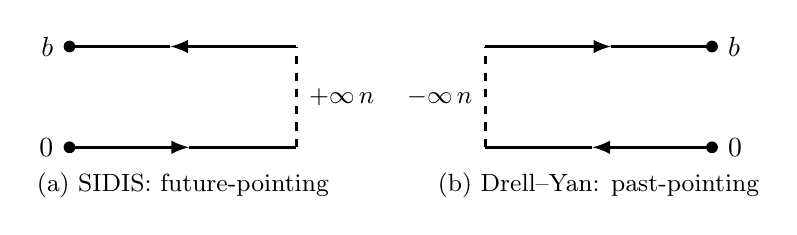
\begin{tikzpicture}[scale=0.8, q/.style={circle, fill=black, inner sep=1.5pt}]
    \begin{scope}[shift={(0,0)}]
      \node[q, label=left:{$0$}] at (0,0) {};
      \node[q, label=left:{$\bvec$}] at (0,1.6) {};
      \draw[very thick, -latex] (0,0) -- (1.9,0);
      \draw[very thick] (1.9,0) -- (3.6,0);
      \draw[very thick, dashed] (3.6,0) -- (3.6,1.6);
      \draw[very thick, -latex] (3.6,1.6) -- (1.6,1.6);
      \draw[very thick] (1.6,1.6) -- (0,1.6);
      \node[right] at (3.65,0.8) {\small $+\infty\,\nminus$};
      \node at (1.8,-0.6) {\small (a) SIDIS: future-pointing};
    \end{scope}
    \begin{scope}[shift={(10.2,0)}]
      \node[q, label=right:{$0$}] at (0,0) {};
      \node[q, label=right:{$\bvec$}] at (0,1.6) {};
      \draw[very thick, -latex] (0,0) -- (-1.9,0);
      \draw[very thick] (-1.9,0) -- (-3.6,0);
      \draw[very thick, dashed] (-3.6,0) -- (-3.6,1.6);
      \draw[very thick, -latex] (-3.6,1.6) -- (-1.6,1.6);
      \draw[very thick] (-1.6,1.6) -- (0,1.6);
      \node[left] at (-3.65,0.8) {\small $-\infty\,\nminus$};
      \node at (-1.8,-0.6) {\small (b) Drell--Yan: past-pointing};
    \end{scope}
  \end{tikzpicture}
  \keymsg{We put this \textbf{staple-shaped link} on the lattice.}
\end{frame}

% Amplitude slices P_L=-2
\begin{frame}{Backup: amplitudes at $P_L=-2$ ($\zetahat=0.294367$), $\eta|v|/a=8$}
  \centering
  \begin{tabular}{cc}
    \includegraphics[height=0.38\textheight, trim=0 0 500 0, clip]{ReA2B_Pb_bsq_eta8_PL-2_2D.pdf} &
    \includegraphics[height=0.38\textheight, trim=0 0 500 0, clip]{ImA2B_Pb_bsq_eta8_PL-2_2D.pdf} \\
    \includegraphics[height=0.38\textheight, trim=0 0 500 0, clip]{ReA12B_Pb_bsq_eta8_PL-2_2D.pdf} &
    \includegraphics[height=0.38\textheight, trim=0 0 500 0, clip]{ImA12B_Pb_bsq_eta8_PL-2_2D.pdf}
  \end{tabular}
\end{frame}

% Amplitude slices P_L=-3
\begin{frame}{Backup: amplitudes at $P_L=-3$ ($\zetahat=0.539684$), $\eta|v|/a=8$}
  \centering
  \begin{tabular}{cc}
    \includegraphics[height=0.38\textheight, trim=0 0 500 0, clip]{ReA2B_Pb_bsq_eta8_PL-3_2D.pdf} &
    \includegraphics[height=0.38\textheight, trim=0 0 500 0, clip]{ImA2B_Pb_bsq_eta8_PL-3_2D.pdf} \\
    \includegraphics[height=0.38\textheight, trim=0 0 500 0, clip]{ReA12B_Pb_bsq_eta8_PL-3_2D.pdf} &
    \includegraphics[height=0.38\textheight, trim=0 0 500 0, clip]{ImA12B_Pb_bsq_eta8_PL-3_2D.pdf}
  \end{tabular}
\end{frame}

% B1
\begin{frame}{Backup: lattice ensemble and $\zetahat$ at $P_L=-1$}
  \begin{columns}[t]
    \begin{column}{0.48\textwidth}
      \begin{block}{From the thesis}
        \begin{itemize}
          \item $n_f=2+1$ clover-improved Wilson fermions (Yoon \emph{et al.} 2017)
          \item $\hat L^3\times\hat T = 32^3\times 96$, \ $a=0.11403$ fm, \ $L\approx3.65$ fm
          \item $m_\pi=317$ MeV
          \item $\mN = 0.6228(28)/a = 1077.8(48)$ MeV
          \item $P_1=-2\pi/L=-339.8$ MeV
          \item Isovector $u-d$, connected contractions
        \end{itemize}
      \end{block}
      % TODO(Hari): m_pi, number of configurations and Jackknife bins, t_snk - t_src, smearing are not stated in the thesis
    \end{column}
    \begin{column}{0.50\textwidth}
      Setting the bracket of the constraint to zero:
      \[ \zetahat =\sqrt{\frac{P_{1}^2}{\mN^{2}\left(\frac{\mN^{2}}{P_{1}^{2}}+2\right)}} = \pm 0.090772 \]
      \[ \zetahat=\frac{-v_{1}P_{1}}{\sqrt{v_{1}^{2}+v_{3}^{2}}\ \mN} \ \Rightarrow\ v_{1}=\pm 0.301\,v_{3} \]
    \end{column}
  \end{columns}
\end{frame}

% B3
\begin{frame}{Backup: the $|\vect b|\ge3a$ cut for $\tAmp_{12B}^{\text{Re}}$}
  \vspace{2mm}
  \centering
  \includegraphics[width=\linewidth]{A12B_Re_b_lessthan3_and_ge3.pdf}
\end{frame}

% B3b
\begin{frame}{Backup: $\tAmp_{12B}^{\text{Im}}$ is consistent with zero}
  \centering
  \includegraphics[width=\linewidth]{ImA12B_Pb_bsq_eta8_PL-3_2D.pdf}\\
  {\scriptsize $\tAmp_{12B}^{\text{Im}}$ at $P_L=-3$, $\eta|v|/a=8$ (all $b^2$, including $|\vect b|<3a$): consistent with zero, so dropped.}
\end{frame}

% B4
\begin{frame}{Backup: PySR benchmark fits}
  \begin{columns}[c]
    \begin{column}{0.62\textwidth}
      \centering
      \includegraphics[height=0.8\textheight, width=\linewidth, keepaspectratio]{01_A2B_PySR_Benchmark_Fits.pdf}
    \end{column}
    \begin{column}{0.36\textwidth}
      \begin{itemize}
        \item Run on $\tAmp_{2B}^{\text{Re}}$ at $P_L=-1$ only.
        \item $\mathcal{P}_{\text{asymptotic}}$ sums $|\tAmp^{\text{model}}|$ at large $b_L$.
        \item Every formula with spatial dependence depends on $b_L, b_T$ only through $b^2$: a guide, not the final model.
      \end{itemize}
    \end{column}
  \end{columns}
\end{frame}

% B5
\begin{frame}{Backup: $c(\eta)$ candidates and the Fourier-transform width}
  \centering
  \includegraphics[height=0.82\textheight, keepaspectratio]{A2BfitFT_eta_Asymptotic_P1.pdf}
\end{frame}

% B5b
\begin{frame}{Backup: $\eta$-independence of $d$, and the $c(\eta)$ choice}
  \begin{columns}[c]
    \begin{column}{0.48\textwidth}
      \centering
      \includegraphics[width=0.9\linewidth]{A2B_d_eta_Independence_P1.pdf}\\
      {\scriptsize $d(\eta)$ for $\tAmp_{2B}^{\text{Re}}$: slope $0.00122(87)$}
    \end{column}
    \begin{column}{0.50\textwidth}
      \begin{itemize}
        \item The $x$-width of $\tAmp_{2B}^{\text{Re}}$ moves with the choice of $c(\eta)$ (previous slide).
        \item $c_2(\eta)=c\big(1-\tfrac{k_1}{\eta}-\tfrac{k_2}{\eta^2}\big)$: lowest AIC, suppresses antiquarks at $x\lesssim-0.2$, consistent with the $x$-integrated results.
        \item The $b_L^2$ coefficient is $d+c_2(\eta)$, which stays positive over $\eta\in[6,10]$.
        % TODO(Hari): state how c(eta) with k1,k2 enters the transform and the zeta-hat extrapolation
      \end{itemize}
    \end{column}
  \end{columns}
\end{frame}

% B6
\begin{frame}{Backup: integrability of the power-law models (remarks, not in thesis)}
  \begin{itemize}
    \item Even amplitudes: $\big[1+C\,(P\cdot b)^2+\ldots\big]^{-j}\sim|P\cdot b|^{-2j}$ $\Rightarrow$ absolutely integrable for $j>1/2$.
    \item $\tAmp_{2B}^{\text{Im}}\propto b_L\,[\ldots]^{-j}\sim|P\cdot b|^{1-2j}$ $\Rightarrow$ absolutely integrable only for $j>1$.
    \item $j_{\text{im}}$ at the simulated momenta $P_L=-1,-2,-3,-4$: \ $1.108(21)$, $1.141(20)$, $1.057(15)$, $1.0084(79)$, all $>1$.
    \item Extrapolated to $\zetahat\to\infty$:
  \end{itemize}
  \[ j_{\text{re}} = 2.0667(69), \quad j_{\text{im}} = 0.9921(92), \quad j_{\text{reA12B}} = 2.0026(40) \]
  \begin{itemize}
    \item At $j_{\text{im}}\approx1$ the sine transform converges only conditionally; this is the sharp structure of $\tAmp_{2B}^{[x]\text{Im}}$ near $x=0$.
    \item Power laws are not entire functions, so support extends beyond $|x|\le1$; numerically $\int_{-\infty}^{\infty}$ and $\int_{-1}^{1}$ agree within errors (next slide).
  \end{itemize}
\end{frame}

% B7
\begin{frame}{Backup: $x$-integrals at $\zetahat\to\infty$, $|\vprp b|=3a$}
  \centering
  \renewcommand{\arraystretch}{1.5}
  {\small
  \begin{tabular}{lcccc}
    \toprule
    Integral & $[-\infty, \infty]$ & $[-1, 1]$ & $[-1, 0]$ & $[0, 1]$ \\
    \midrule
    $\int dx\, \tAmp^{[x]\text{Re}}_{2B}$ & $0.751(79)$ & $0.751(80)$ & $0.375(40)$ & $0.375(40)$ \\
    $\int dx\, \tAmp^{[x]\text{Im}}_{2B}$ & $6(96)\times10^{-17}$ & $3(24)\times10^{-16}$ & $0.165(27)$ & $-0.169(29)$ \\
    $\int dx\, \tilde{f}_1^{(0)}$ & $1.50(16)$ & $1.50(16)$ & $0.421(81)$ & $1.09(11)$  \\
    $\int dx\, \tilde{f}_{1T}^{\perp(1)}$ & $0.302(53)$ & $0.302(53)$ & $0.151(27)$ & $0.151(27)$ \\
    $\mN \int dx\, \tilde{f}_{1T}^{\perp(1)} / \int dx\, \tilde{f}_1^{(0)}$ & $0.217(38)$ & $0.217(38)$ & $0.387(89)$ & $0.150(26)$ \\
    \bottomrule
  \end{tabular}}
  \raggedright
  \begin{itemize}
    \item First four rows are unrenormalized; only the ratio (last row) is quoted as a physical quantity.
    \item The $(-\infty,\infty)$ ratio (last row) equals the $\bvec\tcdot P=0$ ratio (an identity). The content is the split into $[-1,0]$ and $[0,1]$.
  \end{itemize}
\end{frame}

% B8
\begin{frame}{Backup: all twelve parameter extrapolations}
  \centering
  \includegraphics[height=0.8\textheight, keepaspectratio]{Param_Extrapolations_1byZetahat_sq_P234_bmin3_eta610_b29.0.pdf}\\
  {\scriptsize Rows: $\tAmp_{2B}^{\text{Re}}$, $\tAmp_{2B}^{\text{Im}}$, $\tAmp_{12B}^{\text{Re}}$. Each fit: 3 points, 2 parameters.}
\end{frame}

% B9
\begin{frame}{Backup: Sivers shift at the four momenta vs $1/\zetahat$}
  \centering
  \includegraphics[width=0.9\linewidth]{SimulFit_Distinct_1_over_PL_bmin3_eta610_b29.0_Sivers.pdf}
\end{frame}

% B10
\begin{frame}{Backup: extrapolated amplitudes and TMDs}
  \centering
  \includegraphics[height=0.82\textheight, keepaspectratio]{Extrapolated_AmpLevel_P234_Sivers_1_over_zetahat_sq_bmin3_eta610_b29.0_Amps.pdf}
\end{frame}

% B11
\begin{frame}{Backup: full $x$-dependence at $P_L=-3$}
  \centering
  \includegraphics[width=0.75\linewidth]{FT_xdep_A2B_A12B_bmin3_eta610_b2-9_PL-3.pdf}\\
  {\scriptsize Top: $\tAmp^{[x]\text{Re}}_{2B}$, $\tAmp^{[x]\text{Im}}_{2B}$, $\tilde f_1^{(0)}$. Bottom: $\tilde f_{1T}^{\perp(1)}$, $\langle k_y\rangle_{TU}$, $x\langle k_y\rangle_{TU}$.}
\end{frame}

% B12
\begin{frame}{Backup: global fit at $P_L=-3$}
  \centering
  \includegraphics[height=0.82\textheight, keepaspectratio]{Combined_Pb_bsq_eta8_PL-3_WithFit_2D.pdf}
\end{frame}

% B12b
\begin{frame}{Backup: separable models vs the coupled power law}
  \centering
  {\scriptsize
  \renewcommand{\arraystretch}{1.3}\setlength{\tabcolsep}{3.5pt}
  \begin{tabular}{lccccccc}
    \toprule
    Model: longitudinal $\times$ transverse & \multicolumn{4}{c}{$\chi^2/\text{dof}$ at $P_L=-1,-2,-3,-4$} & $c^{\text{Im}}_{2B}$ & $c^{\text{Re}}_{12B}$ & $a^{\text{Im}}_{2B}$ \\
    \midrule
    $e^{-c|P\cdot b|}\times e^{-d|\vect b|}$ & $1.406(92)$ & $0.956(75)$ & $0.622(61)$ & $0.455(53)$ & $0.0010(262)$ & $0.045(23)$ & $-0.167(16)$ \\
    $e^{-c|P\cdot b|}\times(1+d\,b^2)^{-j}$ & $1.286(89)$ & $0.938(75)$ & $0.623(61)$ & $0.447(53)$ & $0.0045(248)$ & $0.028(24)$ & $-0.167(31)$ \\
    $e^{-c(P\cdot b)^2}\times e^{-d|\vect b|}$ & $2.389(121)$ & $2.005(111)$ & $0.945(76)$ & $0.453(52)$ & $0.568(171)$ & $0.0038(69)$ & $+0.050(121)$ \\
    $e^{-c(P\cdot b)^2}\times(1+d\,b^2)^{-j}$ & $2.316(120)$ & $1.981(111)$ & $0.948(76)$ & $0.448(52)$ & $0.602(48)$ & $0.0016(61)$ & $+0.168(92)$ \\
    \midrule
    \textbf{coupled power law in $(P\cdot b, b^2)$} & $1.85(10)$ & $1.197(85)$ & $0.712(66)$ & $0.434(51)$ & $\mathbf{0.2253(69)}$ & $\mathbf{0.0773(46)}$ & $\mathbf{+0.267(13)}$ \\
    \bottomrule
  \end{tabular}}
  \raggedright
  \begin{itemize}
    \item Parameters shown at $P_L=-1$. Separable models: $c^{\text{Im}}_{2B}$ or $c^{\text{Re}}_{12B}$ consistent with zero, $a^{\text{Im}}_{2B}$ sign flips, or poor $\chi^2$.
  \end{itemize}
\end{frame}

% B13a
\begin{frame}{Backup: ratio test directly on lattice data ($P_L=-1$)}
  \centering
  \includegraphics[height=0.82\textheight, keepaspectratio]{Factorization_ratios_Pb034_lin_vs_quad_eta8_PL-1.pdf}
\end{frame}

% B13b
\begin{frame}{Backup: optimal separable factors and reconstruction}
  \centering
  \includegraphics[width=\linewidth]{Factorization_gh_and_Reconstruction_bmin3_eta610.pdf}\\
  {\scriptsize Left: $g(x)$; middle: $h(|\vprp b|)$ for four $x$-windows; right: data vs $g(x)h(|\vprp b|)$ at $|\vprp b|=0.34$ and $0.94$ fm}
\end{frame}

% B14
\begin{frame}{Backup: soft factor and renormalization}
  \begin{itemize}
    \item At fixed geometry: under $\Gamma$-independent multiplicative renormalization, the soft factor and $Z$ cancel in $\tAmp_{12B}/\tAmp_{2B}$ at the same $(\bvec, P, \eta v)$.
    \item This work: ratios of amplitudes at fixed geometry, with $\bvec\tcdot P$ scanned and Fourier transformed.
    \item The $(-\infty,\infty)$ entry of the last row of the integral table equals the $\bvec\tcdot P=0$ ratio (an identity).
    % TODO(Hari): prepare the oral answer on what changes with b_L at fixed |b_T| (link length vs cusp angles)
  \end{itemize}
\end{frame}

% B15
\begin{frame}{Backup: generalized shifts of other TMDs}
  \small
  \begin{align*}
    \langle \vect{k}_y \rangle_{UT}(\vprp{\bvec}^2,x)
      &= \mN \frac{\int d(\bvec\tcdot P)\, e^{ix(\bvec\tcdot P)}\, \tAmp_{4B}}{\int d(\bvec\tcdot P)\, e^{ix(\bvec\tcdot P)}\, \tAmp_{2B}} & &\text{(Boer--Mulders, T-odd)} \\
    \langle \vect{k}_x \rangle_{TL}(\vprp{\bvec}^2,x)
      &= -\mN \frac{\int d(\bvec\tcdot P)\, e^{ix(\bvec\tcdot P)}\, \tAmp_{7B}}{\int d(\bvec\tcdot P)\, e^{ix(\bvec\tcdot P)}\, \tAmp_{2B}} & &\text{(worm-gear $g_{1T}$, T-even)} \\
    \frac{\tilde h_{1}^{(0)}}{\tilde f_1^{(0)}}(\vprp{\bvec}^2,x)
      &= -\frac{\int d(\bvec\tcdot P)\, e^{ix(\bvec\tcdot P)}\, \tAmp_{9Bm}}{\int d(\bvec\tcdot P)\, e^{ix(\bvec\tcdot P)}\, \tAmp_{2B}} & &\text{(tensor charge, T-even)}
  \end{align*}
  \normalsize
  \begin{itemize}
    \item Unlike the $x$-integrated shifts ($\bvec\tcdot P=0$ only), each needs a scan in $\bvec\tcdot P$ under the same kinematic constraint.
  \end{itemize}
\end{frame}


\end{document}
